% Options for packages loaded elsewhere
\PassOptionsToPackage{unicode}{hyperref}
\PassOptionsToPackage{hyphens}{url}
%
\documentclass[
  a5paper,
  smalldemyvopaper,10pt,twoside,onecolumn,openright,extrafontsizes,hidelinks]{memoir}

\usepackage{amsmath,amssymb}
\usepackage{iftex}
\ifPDFTeX
  \usepackage[T1]{fontenc}
  \usepackage[utf8]{inputenc}
  \usepackage{textcomp} % provide euro and other symbols
\else % if luatex or xetex
  \usepackage{unicode-math}
  \defaultfontfeatures{Scale=MatchLowercase}
  \defaultfontfeatures[\rmfamily]{Ligatures=TeX,Scale=1}
\fi
\usepackage{lmodern}
\ifPDFTeX\else  
    % xetex/luatex font selection
\fi
% Use upquote if available, for straight quotes in verbatim environments
\IfFileExists{upquote.sty}{\usepackage{upquote}}{}
\IfFileExists{microtype.sty}{% use microtype if available
  \usepackage[]{microtype}
  \UseMicrotypeSet[protrusion]{basicmath} % disable protrusion for tt fonts
}{}
\makeatletter
\@ifundefined{KOMAClassName}{% if non-KOMA class
  \IfFileExists{parskip.sty}{%
    \usepackage{parskip}
  }{% else
    \setlength{\parindent}{0pt}
    \setlength{\parskip}{6pt plus 2pt minus 1pt}}
}{% if KOMA class
  \KOMAoptions{parskip=half}}
\makeatother
\usepackage{xcolor}
\setlength{\emergencystretch}{3em} % prevent overfull lines
\setcounter{secnumdepth}{5}
% Make \paragraph and \subparagraph free-standing
\makeatletter
\ifx\paragraph\undefined\else
  \let\oldparagraph\paragraph
  \renewcommand{\paragraph}{
    \@ifstar
      \xxxParagraphStar
      \xxxParagraphNoStar
  }
  \newcommand{\xxxParagraphStar}[1]{\oldparagraph*{#1}\mbox{}}
  \newcommand{\xxxParagraphNoStar}[1]{\oldparagraph{#1}\mbox{}}
\fi
\ifx\subparagraph\undefined\else
  \let\oldsubparagraph\subparagraph
  \renewcommand{\subparagraph}{
    \@ifstar
      \xxxSubParagraphStar
      \xxxSubParagraphNoStar
  }
  \newcommand{\xxxSubParagraphStar}[1]{\oldsubparagraph*{#1}\mbox{}}
  \newcommand{\xxxSubParagraphNoStar}[1]{\oldsubparagraph{#1}\mbox{}}
\fi
\makeatother


\providecommand{\tightlist}{%
  \setlength{\itemsep}{0pt}\setlength{\parskip}{0pt}}\usepackage{longtable,booktabs,array}
\usepackage{calc} % for calculating minipage widths
% Correct order of tables after \paragraph or \subparagraph
\usepackage{etoolbox}
\makeatletter
\patchcmd\longtable{\par}{\if@noskipsec\mbox{}\fi\par}{}{}
\makeatother
% Allow footnotes in longtable head/foot
\IfFileExists{footnotehyper.sty}{\usepackage{footnotehyper}}{\usepackage{footnote}}
\makesavenoteenv{longtable}
\usepackage{graphicx}
\makeatletter
\def\maxwidth{\ifdim\Gin@nat@width>\linewidth\linewidth\else\Gin@nat@width\fi}
\def\maxheight{\ifdim\Gin@nat@height>\textheight\textheight\else\Gin@nat@height\fi}
\makeatother
% Scale images if necessary, so that they will not overflow the page
% margins by default, and it is still possible to overwrite the defaults
% using explicit options in \includegraphics[width, height, ...]{}
\setkeys{Gin}{width=\maxwidth,height=\maxheight,keepaspectratio}
% Set default figure placement to htbp
\makeatletter
\def\fps@figure{htbp}
\makeatother

% typographical packages
\usepackage{microtype}
\usepackage{setspace}
\tolerance=6000
\hyphenpenalty=1000

% typographical settings for the body text
\setlength{\parskip}{0em}
\setlength{\parindent}{1em}
\linespread{1.3}

% DEFINITIONS TITLE PAGE / COPYRIGHT
\newcommand{\titleoriginal}{Title}
\newcommand{\subtitleoriginal}{Subtitle}
\newcommand{\yearoriginal}{Year}
\newcommand{\subtitletranslation}{Translation Subtitle}
\newcommand{\yeartranslation}{Translation Year}
\newcommand{\stringtranslation}{Translation String}
\newcommand{\stringlicense}{Translation License String.}
\newcommand{\stringpublisher}{Published by String}
\newcommand{\ISBNHC}{978-9916-}
\newcommand{\ISBNSC}{978-9916-}
\newcommand{\ISBNEBOOK}{978-9916-}
%\newcommand{\ISBNAUDIO}{978-9916-}
\newcommand{\press}{Konsensus Network}
\newcommand{\translatorone}{Translator 1}
\newcommand{\translators}{
\large\textit{\stringtranslation:}\\
\translatorone\\
}

% PHYSICAL DOCUMENT SETUP
\setstocksize{210mm}{148mm}
\settrimmedsize{210mm}{148mm}{*}
\setbinding{5mm}
\setlrmarginsandblock{8mm}{15mm}{*}
\setulmarginsandblock{25mm}{26mm}{*}

% FONTS
\usepackage{fontspec}
\setmainfont{stone-serif}[
    Path=./fonts/stone-serif-itc-pro/,
    Scale=0.86,
    Extension=.OTF,
    UprightFont=*-Regular,
    BoldFont=*-SemiBd,
    ItalicFont=*-MediumIt,
    BoldItalicFont=*-SemiBdIt
    ]

\setsansfont{stone-sans}[
    Path=./fonts/stone-sans/,
    Scale=0.82,
    Extension=.otf,
    UprightFont=*-Medium,
    BoldFont=*-Semibold,
    ItalicFont=*-MediumItalic,
    BoldItalicFont=*-SemiBoldItalic
    ]

\usepackage{lettrine}
\setcounter{DefaultLines}{3}
\renewcommand{\DefaultLoversize}{0.1}
\renewcommand{\DefaultLraise}{0}
\renewcommand{\LettrineTextFont}{}
\setlength{\DefaultFindent}{\fontdimen2\font}
\setlength{\DefaultNindent}{0em}

%\usepackage[footskip=8mm]{geometry}

% custom second title page
\makeatletter
\newcommand*\halftitlepage{\begingroup % Misericords, T&H p 153
  \setlength\drop{0.1\textheight}
  \begin{center}
  \vspace*{\drop}
  \rule{\textwidth}{0in}\par
  {\Large\sffamily\thetitle\par}
  \rule{\textwidth}{0in}\par
  \vfill
  \end{center}
\endgroup}
\makeatother

% custom title page
\makeatletter
\newlength\drop
\newcommand*\titleM{\begingroup % Misericords, T&H p 153
  \setlength\drop{0.15\textheight}
  \begin{center}
  \vspace*{\drop}
  {\huge\sffamily\thetitle\par}
  \vspace{2em}
  %{\normalsize\sffamily\textit\subtitletranslation\par}
  %\vspace{2em}
  \rule{5.5cm}{0.3mm}\par
  \vspace{2em}
  {\Large\sffamily\textit\theauthor\par}
  \vspace{3em}
  %{\footnotesize\sffamily\textit\translators\par}
  \vfill
  
\includegraphics[width=3.5cm]{figures/knw.png}\par
  \end{center}
\endgroup}
\makeatother

% copyright page
\makeatletter
\newcommand*\copyrightpage{\begingroup
  \setlength\drop{0.1\textheight}
  \vphantom{just for the drop}
  \vfill
  \begin{scriptsize}
  \noindent \copyright\space \yearoriginal: \theauthor
  \par\noindent \textit{\titleoriginal}
  \vspace{0.5\baselineskip}
  %\par\noindent \copyright\space \yeartranslation\space \stringtranslation: \translatorone
  %\par\noindent \textit{\thetitle: \subtitletranslation}
  \vspace{\baselineskip}
  \par\noindent \textit{\stringlicense}
  \vspace{0.5\baselineskip}
  \par\noindent \stringpublisher: \href{https://konsensus.network}{\textit{konsensus.network}}
  \vspace{0.5\baselineskip}
  \par\noindent v1.0.0
  \vspace{0.5\baselineskip}
  \setlength{\parindent}{2em}% default 20pt
  \par\noindent ISBN \ISBNHC \:Hardcover
  \par\hspace{0.28\parindent}\ISBNSC \:Paperback
  \par\hspace{0.28\parindent}\ISBNEBOOK \:E-book\par
  \setlength{\parindent}{0pt}
  \end{scriptsize}
  \vspace{3em}
  \par\noindent \href{https://konsensus.network}{\large\MakeUppercase \press \hspace{3em} 
\includegraphics[width=1cm]{figures/freestarfish.png}}
  \setcounter{footnote}{0}
  \clearpage
\endgroup}
\makeatother

% HEADER AND FOOTER MANIPULATION
% for normal pages
\nouppercaseheads
\headsep = 10mm
\makepagestyle{mystyle} 
\makeevenhead{mystyle}{\scriptsize\sffamily\mdseries\thepage}{}{}
\makeoddhead{mystyle}{{\scriptsize\sffamily\mdseries\leftmark}}{}{\scriptsize\sffamily\mdseries\thepage}
\makeevenfoot{mystyle}{}{}{}
\makeoddfoot{mystyle}{}{}{}
\makeatletter

% for pages where chapters begin
\makepagestyle{plain}
\makerunningwidth{plain}{\headwidth}
\makeevenfoot{plain}{}{}{}
\makeoddfoot{plain}{}{\scriptsize\sffamily\mdseries\thepage}{}
\pagestyle{mystyle}

\newif\ifmainmatter
\appto\mainmatter{\mainmattertrue}
\appto\backmatter{\mainmatterfalse}
\appto\appendix{\mainmatterfalse}

\renewcommand\chaptermark[1]{%
  \markboth{\MakeUppercase{%
    \ifmainmatter~\oldstylenums\thechapter.~\fi#1}}{}}%

% TOC
\usepackage[]{tocloft}
\renewcommand{\cftsectiondotsep}{\cftnodots}
\renewcommand{\cftpartfont}{\Large\sffamily\MakeUppercase}
\renewcommand{\cftchapterfont}{\small\sffamily}
\renewcommand{\cftsectionfont}{\Small\sffamily}
\renewcommand{\cftpartpagefont}{\Large\sffamily}
\renewcommand{\cftchapterpagefont}{\small}
\renewcommand{\cftchapterpresnum}{HOOFDSTUK\space}
\renewcommand{\cftchapternumwidth}{7em}
\setlength{\cftchapterindent}{0em}
\setlength{\cftsectionindent}{7em}
\setlength{\cftbeforechapterskip}{-0.2em}
\setsecnumdepth{chapter}
\setcounter{tocdepth}{0}


% Redefine footnote presentation
\makeatletter
\renewcommand\@makefntext[1]{%
  \noindent\hb@xt@2em{% <-- Box of fixed size for footnote number and space
    \@thefnmark\quad}% <-- Footnote number followed by a quad space
  \parbox[t]{\dimexpr\linewidth-2em}{#1}% <-- Parbox to control the width of footnote content
}
\makeatother

% layout check and fix
\checkandfixthelayout

% COUNTERS FOOTNOTES
\usepackage{chngcntr}
\counterwithout*{footnote}{chapter}

% TITLE FORMATTING
\usepackage{titlesec}
\titleformat
    {\chapter}[display]
    {\huge\sffamily}
    {\Large\sffamily\chaptertitlename\space\thechapter}
    {0pt}
    {\vspace{28pt}}

\titleformat
  {\section}[block]
  {\sffamily\large\bfseries}
  {}
  {0pt}
  {}
  
\titlespacing*{\section}{0pt}{2em}{0.5em}

\titleformat{\subsection}{\sffamily\bfseries}{}{}{}
\titlespacing*{\subsection}{0pt}{2em}{0em}

% QUOTE FORMATTING
\renewenvironment{quote}%
               {\list{}{\rightmargin=.6cm\leftmargin=.6cm}%
                \itshape \item[]}% <- The effect of \samepage is local!!!
               {\endlist}

% LAYOUT CHECK AND FIX
\checkandfixthelayout

% CUSTOM TITLE PAGE
\makeatletter
\def\@maketitle{%
  % the half title page
  \pagestyle{empty}
  \halftitlepage
  \cleardoublepage

  % the title page
  \titleM
  \clearpage

  % the copyright page
  \copyrightpage
  \cleardoublepage
  \pagestyle{mystyle}
}
\makeatother
% END PREAMBLE
\makeatletter
\@ifpackageloaded{bookmark}{}{\usepackage{bookmark}}
\makeatother
\makeatletter
\@ifpackageloaded{caption}{}{\usepackage{caption}}
\AtBeginDocument{%
\ifdefined\contentsname
  \renewcommand*\contentsname{Table of contents}
\else
  \newcommand\contentsname{Table of contents}
\fi
\ifdefined\listfigurename
  \renewcommand*\listfigurename{List of Figures}
\else
  \newcommand\listfigurename{List of Figures}
\fi
\ifdefined\listtablename
  \renewcommand*\listtablename{List of Tables}
\else
  \newcommand\listtablename{List of Tables}
\fi
\ifdefined\figurename
  \renewcommand*\figurename{Figure}
\else
  \newcommand\figurename{Figure}
\fi
\ifdefined\tablename
  \renewcommand*\tablename{Table}
\else
  \newcommand\tablename{Table}
\fi
}
\@ifpackageloaded{float}{}{\usepackage{float}}
\floatstyle{ruled}
\@ifundefined{c@chapter}{\newfloat{codelisting}{h}{lop}}{\newfloat{codelisting}{h}{lop}[chapter]}
\floatname{codelisting}{Listing}
\newcommand*\listoflistings{\listof{codelisting}{List of Listings}}
\makeatother
\makeatletter
\makeatother
\makeatletter
\@ifpackageloaded{caption}{}{\usepackage{caption}}
\@ifpackageloaded{subcaption}{}{\usepackage{subcaption}}
\makeatother

\ifLuaTeX
\usepackage[bidi=basic]{babel}
\else
\usepackage[bidi=default]{babel}
\fi
\babelprovide[main,import]{english}
\babelprovide[import]{greek}
% get rid of language-specific shorthands (see #6817):
\let\LanguageShortHands\languageshorthands
\def\languageshorthands#1{}
\ifLuaTeX
  \usepackage{selnolig}  % disable illegal ligatures
\fi
\usepackage{bookmark}

\IfFileExists{xurl.sty}{\usepackage{xurl}}{} % add URL line breaks if available
\urlstyle{same} % disable monospaced font for URLs
\hypersetup{
  pdftitle={L'Élégance de Bitcoin},
  pdfauthor={Ludovic Lars},
  pdflang={en},
  hidelinks,
  pdfcreator={LaTeX via pandoc}}


\title{L'Élégance de Bitcoin}
\author{Ludovic Lars}
\date{2024-01-31}

\begin{document}
\frontmatter
\maketitle

\renewcommand*\contentsname{Contents}
{
\setcounter{tocdepth}{0}
\tableofcontents
}

\mainmatter
\bookmarksetup{startatroot}

\chapter*{À propos de ce livre}\label{uxe0-propos-de-ce-livre}
\addcontentsline{toc}{chapter}{À propos de ce livre}

\markboth{À propos de ce livre}{À propos de ce livre}

\bookmarksetup{startatroot}

\chapter*{Preface by Jacques Favier}\label{pruxe9face-de-jacques-favier}
\addcontentsline{toc}{chapter}{Preface by Jacques Favier}

\markboth{Preface by Jacques Favier}{Preface by Jacques Favier}

Ludovic Lars is widely regarded as one of the foremost French-speaking
``scholars'' on Bitcoin. This term, which surfaced in several
conversations about his publishing project, inspired the theme of this
preface.

When he honored me by requesting this preface, he cautioned that the
``liberal'' tone of his \emph{Elegance of Bitcoin} might contrast with
my own sensibilities. Yet, I perceived in it a kind of moral
\emph{elegance}. Indeed, the author has read both the so-called
``Austrian'' economists and Proudhon, and he is no more a stubborn or
toxic maximalist than I am. As someone who opposes ideological
extremisms and one-dimensional reasoning, I cannot be offended that
within a community advocating for decentralized solutions, differing
opinions prevail, along with their inherent visions and biases.

Embracing what one might once have called a true ``Benedictine labor,''
the author sought and gained the trust of numerous specialists who
ensured that his work incorporated a broad spectrum of knowledge and
received meticulous review. Beyond this collaboration of experts, there
was a genuine communal, financial, and moral commitment to bring this
book to publication.

Thus, we encounter here a work that, through its seldom polemical tone,
profound erudition, and integration into a collective movement,
participates in the tradition of the French \emph{Encyclopedia}. It is
known that the promoters of the \emph{Britannica} accused Diderot and
d'Alembert's encyclopedia of ``spreading anarchy,'' and it cannot be
denied that, composed during the blossoming of the Enlightenment, this
compendium of all kinds of knowledge---both theoretical and
practical---courageously took sides in the political and philosophical
struggles of its time, explicitly intending to foster critical
reflection and ``change the common way of thinking.'' Perhaps the same
can be said here: Bitcoin and this book invite you not merely, or not
only, to change currency but to change thought.

Perceiving this connection, I delved into the \emph{Encyclopedia}. The
article on ``Erudition,'' penned by d'Alembert himself, states that it
``encompasses three principal branches: the knowledge of History, of
Languages, and of Books.'' By perhaps substituting \emph{languages} with
\emph{protocols}, he might also have appreciated---and prefaced better
than I---the book you are about to open.

My own mind, shaped by historical studies, reveled in the initial
chapters, which form veritable Annals of Bitcoin. Historians of today
and the future will surely value the extensive reliable information and
compiled references. As a mathematician by training, the author first
produced a substantial archival work, evidenced by nearly a thousand
scholarly footnotes.

As the creator of Bitcoin.fr wrote to me, ``He uncovers and deciphers
obscure debates that nonetheless played a crucial role in the evolution
of the protocol, making them understandable to all.'' Therefore, while
his presentation of monetary history might be critiqued or reframed in
light of his personal convictions, his construction of Bitcoin's history
is a contribution from which others will beneficially draw.

Beyond History, there are the Languages and the Books: references, code,
game theory, and mathematics. There is much to harvest in these
pages---many austere subjects, but also delightful anecdotes. While the
book details the inevitable story of the famous pizza, it also reminds
us that a Bitcoin faucet operated for two years, dispensing 5 bitcoins
upon each request, or that the individual who discovered the first flaw
graciously informed Satoshi instead of exploiting his discovery to
cheat. It highlights that before its phase of ``conflictual growth,''
the early years of the venture saw ``organic and cautious growth,
protected from the opportunism and propaganda of our world,'' and that
the community has exhibited, from the very beginning, extraordinary
resilience---something worthy of contemplation.

The wealth of quotations does justice to the cypherpunks, sometimes
depicted as sinister figures fomenting a tax revolt over an ill-timed
barbecue. It restores the historical and intellectual depth of what was
a collective grassroots movement, not a superficial sectarian reaction.
Furthermore, the meticulously retraced individual paths demonstrate that
Austrian influence, though significant, was neither universal nor
absolute. Many cryptographers, cypherpunks or otherwise, did not embrace
it as a revealed dogma or a scientifically established truth.

Ludovic Lars also underscores this crucial point: the cypherpunks were
not alone in trying to construct distributed systems capable of
facilitating monetary exchange---because there was a genuine problem and
a genuine need. Amid the intellectual ferment, exchanges were plentiful;
it is amusing to recall that Ripple was also inspired by the localism of
LETS schemes! In fact, what sets Bitcoin apart from all other attempts
is that it---the first not to rely on trust in the classical
sense---succeeded as a currency because it managed to build an elective,
philosophical, and political community. Bitcoin is the largest community
currency of all time.

Thus, delving into its long saga both before and after 2009 is not
merely a historian's whim. Beyond gaining essential insight into its
roots, the intentions, and ambitions that motivated its precursors and
those who witnessed its birth, one finds ample material to debunk many
persistent intellectual deceits. No, central bank digital currencies or
algorithmic stablecoins do not represent refinements of Bitcoin, nor do
they promise improvements to our future existence.

The various altcoins---somewhat community-driven, often entrepreneurial
or even banking---are extensively cited, primarily to illustrate the
discussion, enrich it with examples, and highlight dead ends or
objections. Never, it bears repeating, and even though the author is
well acquainted with them, is the aim to ``surpass'' or ``perfect''
Bitcoin, whose organic development and refinement is the concern of
bitcoiners.

The author is a technical expert, yet he also knows how to write. All
that is technical (and overlooked by many people, even those who present
themselves as ``experts'')---everything that d'Alembert would term ``the
Languages''---is dissected in this work with an extremely meticulous
scalpel and rendered in the language where what is well conceived ``is
stated clearly.'' This deserves to be given to the next politician,
financier, economist, or commentator who claims that ``it rests on
nothing''!

The title of the book is also that of a pleasantly balanced conclusion
between those who see Bitcoin as the panacea and those who view it
solely negatively. It may surprise some fervent and naïve adherents, but
it remains in the spirit of d'Alembert: ``In criticism, there are two
extremes to equally avoid, too much indulgence and too much severity.''

Curiously, the author dwells little on the word \emph{elegance} itself,
which his mathematical background perhaps leads him to perceive as
encompassing truth, beauty, and rigor. Like Aristotle, he may have
contemplated order, precision, and the ability to harmonize multiple
concepts, adjusting them effectively together---a feat that Satoshi
Nakamoto achieved at the highest level.

To address the reader at the threshold of this useful, dense, and
distinguished book, I once again give the floor to d'Alembert, who
opined that ``the assistance we have today for erudition facilitates it
so much that our laziness would be inexcusable if we did not take
advantage of it.''

Jacques Favier, November 21, 2023

\bookmarksetup{startatroot}

\chapter*{Acknowledgments}\label{remerciements}
\addcontentsline{toc}{chapter}{Acknowledgments}

\markboth{Acknowledgments}{Acknowledgments}

No book is ever solely the result of its author's efforts. Behind every
author are those who help, fund, encourage, and inspire. The book you're
holding, or viewing on a screen, is no exception. I would like to
express my gratitude to everyone who has assisted me in one way or
another, especially the French-speaking Bitcoin community who supported
this project.

First and foremost, I thank my readers for reading and sharing my
articles. A creator is nothing without an audience. I am particularly
grateful to JohnOnChain for his early support of my writing journey. My
thanks also go to the teams behind Cryptoast and Journal du Coin, with
whom I've had the pleasure of working for years.

I am grateful to those who helped launch the funding campaign in March
2022. Thank you to Lounès Ksouri for his advice about Umbrel. Thank you
to Benjamin Favre for helping set up the campaign on the server. Thank
you to CryptoSou for providing me with Lightning liquidity when I needed
it.

I extend my gratitude to the project's financial contributors, listed in
alphabetical order: Yanis Adoul, Autrement, Valentin Becmeur,
Bitcoin.fr, btcfork, Caulla, Chamigrou, Copinmalin, CryptoSou, Steve
Deplus, Marek Fijalkowski, Édouard Gallego, Alexandre Gonzalez,
Gladsponk, Greglem, Grittoshi, Benoît Huguet, ImTechnicolor,
Jacques-Edouard, Jazaronaut, Lionel Jeannerat, Jeffbeck, JohnOnChain,
Clément Junca, François Juno, Jybe, Kolkoz, Mike Komaransky, Konohime,
Maxime Kouamen, Lounès Ksouri, Leslie, Louferlou, Marco.BTC.fr, Loïc
Morel, Ali Mitchell, Yorick de Mombynes, Nexus 8, Leonardo Noleto,
Olivier, Romain Pariset-Wagnon, PaulADW, Pivi, RaHaN, Anthony Ro₿in,
Robin from Cryptoast, Rogzy, Thibaut Spanier, André Stilmant,
François-Xavier Thoorens, Trigger, as well as all those who wished to
remain anonymous.

I am grateful to the reviewers of the initial drafts of this book, who
offered valuable advice to improve it, both in terms of style and
substance. Thank you to Jybe, ProfEduStream, Loïc Morel, Steve Deplus,
Alexandre Gonzalez, Romain Daubigny (Recktosaurus), Pierre L. (aka
Scrypto), Jacques-Edouard from BTC Touchpoint, Bastien Desteuque,
Cédric, Meffysto, Beemo, Caroline and Marie-Christine, Gloire
Wanzavalere, Gatien, and Martin Pellemoine.

I am deeply appreciative of the team at Konsensus, the specialized
publishing house releasing this book. My profound thanks to Édouard
Gallego for his unwavering support in editing this work. Thank you also
to David St-Onge for his editorial guidance. Additionally, I am grateful
to the talented illustrator ImTechnicolor, who created the cover.

I am deeply thankful to Jacques Favier, co-founder of Le Cercle du Coin
and co-author of three books on Bitcoin in French, who honored me by
reading the entire work and writing a superb preface.

I, of course, pay tribute to Satoshi Nakamoto for creating Bitcoin and
sharing it with the world. I also extend my thanks to everyone who has
helped me deepen my understanding of Bitcoin over time, especially
Andreas Antonopoulos, Julia Tourianski, Eric Voskuil, and Aaron van
Wirdum.

Lastly, I thank my loved ones---my family and friends---who provided
essential support during these long months of writing and revision.

\bookmarksetup{startatroot}

\chapter*{Preface}\label{avant-propos}
\addcontentsline{toc}{chapter}{Preface}

\markboth{Preface}{Preface}

Since its inception in 2008 by Satoshi Nakamoto, Bitcoin has sparked
extensive discussion. Over the years, it has ignited intense passions
and been the subject of numerous heated debates. Thousands of articles
have been written, hundreds of videos produced, and dozens of books
published on the topic. The surge in its price has granted it
extraordinary media visibility, embedding it into the global collective
imagination.

Yet, Bitcoin remains widely misunderstood. Many speak of it with only a
superficial grasp, failing to discern its true utility. Some believe it
serves merely for speculation; others imagine it is used exclusively by
criminals; and some even assert that it is nothing more than a Ponzi
scheme. Conversely, a number of individuals harbor unrealistic
expectations, thinking it could become the world's reserve currency or
even replace all monetary exchanges in the economy within a few years.
Immersed in this delusion, they cling to the hope that its price will
reach astronomical levels, continuing the speculative rises of the past.
However, few attempt to adopt a realistic and sober perspective that
balances the dreamers' vision---who see Bitcoin as the solution to all
the world's problems---with the disingenuous detractors who consider
Bitcoin a scourge to be halted at all costs.

I first learned about Bitcoin in April 2013, following the Cypriot
financial crisis. Initially quite skeptical, I nonetheless took an
interest in the system, as it was highlighted by the French liberals and
American libertarians I followed. On July 9, 2015, I decided to give it
a try: I acquired €50 worth of bitcoins (0.2\,BTC) from the Swiss
exchange platform Fastcoin (now known as Bity), which I received in my
newly created Electrum wallet. That day, I made my first transaction on
the Bitcoin blockchain. These few fractions of bitcoin allowed me to
make donations: first to the blogger H16, then to activist Adam Kokesh,
followed by the DarkWallet project by Amir Taaki and Cody Wilson, and
finally to the Sci-Hub platform managed by Alexandra Elbakyan.

My real involvement with Bitcoin began in the spring of 2017, when the
price started to rise again after years of stagnation. Until then, I had
merely followed the cryptocurrency from a distance, and this increase
piqued my interest. It was at that moment that I fully immersed myself
in this world. I read extensively on the subject, acquiring works such
as \emph{Bitcoin, la monnaie acéphale} by Adli Takkal-Bataille and
Jacques Favier, \emph{Mastering Bitcoin} by Andreas Antonopoulos, and
\emph{Digital Gold} by Nathaniel Popper. I also began speculating on a
modest scale by purchasing bitcoin and various alternative
cryptocurrencies.

Simultaneously, I started writing on the topic, eventually becoming a
contributor for specialized sites like Cryptoast and Journal du Coin.
Over the years, I have written more than 150 in-depth articles on
various subjects related to cryptocurrency, whether from a technical,
economic, or political perspective. My understanding of Bitcoin matured
accordingly, to the point where I could claim to ``understand Bitcoin,''
even if my conception remained, of course, partial and influenced by my
own perspective.

However, this was not necessarily the case among those around me, who
had only a superficial idea and likely lacked the time to delve deeper.
This motivated me to write this book. In particular, since the monetary
protocol depends on the economic actions of its users, it seemed
important to share the genuine knowledge that emerged from my research
and experience. Moreover, with the progression of banking censorship,
the development of central bank digital currencies, the war on cash, and
the return of inflation, I believe it is more essential than ever to
fully grasp this tool to use it effectively in the future.

This work aims to present Bitcoin in a clear and comprehensive manner,
adopting multiple viewpoints. It narrates the long journey that led to
its creation, as well as its brief but dense history from its origins to
the present day. It describes its essentially economic functioning
stemming from its monetary nature. It addresses the political issues
Bitcoin responds to, particularly the problem of censorship. Finally, it
examines its technical mechanisms in detailed and precise terms. By
reading this book, you may perhaps, like me, come to see Bitcoin as a
harmonious whole, whose foundational model possesses a rare elegance.

I hope you will appreciate this modest contribution to something that
transcends us all: the project of an alternative, free, and resilient
currency, offering ordinary individuals the ability to resist the powers
of this world. \emph{Vires in numeris}.

Ludovic Lars, December 1, 2023

\bookmarksetup{startatroot}

\chapter{The Beginnings of Bitcoin}\label{ch:mythe}

\phantomsection\label{enotezch:1}{}

{[}Lettrine L{]}{[}Smallcaps e{]} On October 31, 2008, an individual
calling himself Satoshi Nakamoto shared a brief document online that
described the technical workings of an innovative digital currency
system: Bitcoin. This nine-page white paper, presented as a scientific
article, was titled \emph{Bitcoin: A Peer-to-Peer Electronic Cash
System}. In it, Satoshi proposed a solution to the problem of online
payments by implementing a distributed timestamp server based on a
proof-of-work algorithm.

But it went much further. The Bitcoin white paper laid the groundwork
for a profound conceptual revolution: a purely digital currency that
relied on no trusted third party, neither for transaction confirmation
nor for the issuance of new units. What Satoshi had just discovered was
much more than a payment system; it was a new type of money, something
no one had been able to conceive until then---an economic and social
phenomenon that would achieve unprecedented success in the years to
follow.

In particular, Satoshi Nakamoto's creation realized the long-held dream
of a digital currency escaping state control---a dream cherished by the
cypherpunks. Dating back to the early 1990s, this movement advocated the
proactive use of cryptography to ensure individual privacy and freedom
on the internet. These rebellious cryptographers had long desired and
attempted to design such electronic cash, as it was a fundamental part
of their ideal. Unfortunately, these efforts had not succeeded, at least
until the emergence of Bitcoin.

From that pivotal date, Bitcoin was implemented and experienced a series
of foundational events that led it to where it is today. These events
shaped our understanding of it, and the story of Bitcoin's early days is
therefore a unique narrative worth recounting.

\section*{A Difficult Birth}\label{une-naissance-difficile}
\addcontentsline{toc}{section}{A Difficult Birth}

\markright{A Difficult Birth}

Bitcoin was conceived by an individual using the pseudonym Satoshi
Nakamoto, who claimed to be a 33-year-old Japanese man\footnote{Some
  believe Satoshi Nakamoto was a pseudonym used by a group. However,
  we'll assume here that a single person was behind the messages and
  code attributed to Bitcoin's creator, without denying possible
  assistance.}. Little is known about him beyond his public messages and
the computer code he published. Satoshi disappeared in 2011, and it is
unknown whether he is still alive.

According to his own account, Satoshi Nakamoto began working on Bitcoin
in the spring of 2007. For more than a year, he kept his model secret,
wanting to ensure it worked correctly before presenting it to the world.
He would later claim to have coded the prototype before writing the
paper\footnote{Satoshi Nakamoto, \emph{Bitcoin P2P e-cash paper},
  11/09/2008 01:58:48 UTC:
  \url{https://www.metzdowd.com/pipermail/cryptography/2008-November/014832.html}.}.

In August 2008, Satoshi finished drafting the white paper and began
preparing to announce Bitcoin's release. On August 18, he registered the
domain name Bitcoin.org via the anonymous service
AnonymousSpeech\footnote{Satoshi also registered the domain Netcoin.org
  around the same time, suggesting he hadn't finalized his choice of
  name.---Or Weinberger on Twitter, 09/23/2022 08:54 UTC:
  \url{https://twitter.com/orweinberger/status/1573234325046558720}.}.
The domain would be used to host Bitcoin's main website.

A few days later, he contacted Adam Back, the British cryptographer and
cypherpunk behind Hashcash, the technique used in Bitcoin to compute the
proof of work. Adam Back referred him to the cryptographer Wei Dai, the
inventor of the b-money concept in 1998---a concept with notable
similarities to Bitcoin. On August 22, Satoshi emailed Wei Dai to tell
him he was ``getting ready to release a paper that expands on {[}his{]}
ideas into a fully working system'' and to ask him ``the publication
year of {[}his{]} b-money page'' to reference it in the white
paper\footnote{Gwern Branwen, \emph{Wei Dai/Satoshi Nakamoto 2009
  Bitcoin emails}, March 17, 2014:
  \url{https://gwern.net/doc/bitcoin/2008-nakamoto}.}. However, despite
these interactions, Adam Back and Wei Dai did not immediately take
interest in Bitcoin. It would be years later before they revisited this
revolutionary discovery by the mysterious figure.

In the fall of 2008, Satoshi decided to make his system public. On
October 5, he registered on the project management platform SourceForge,
where Bitcoin's open-source code would be hosted and maintained until
2011. On October 31, he published the white paper on a cryptography
mailing list. This list, the Metzdowd Cryptography Mailing List managed
by Perry Metzger on his website Metzdowd.com, included participation
from several former cypherpunks\footnote{Archives of the Metzdowd
  mailing list are publicly available at
  \url{https://www.metzdowd.com/pipermail/cryptography/}. Cypherpunks
  present in 2008 included John Gilmore, Hal Finney, James A. Donald,
  Robert Hettinga, Zooko Wilcox-O'Hearn, and Len Sassaman.}. In his
introductory email, he wrote:

``I've been working on a new electronic cash system that's fully
peer-to-peer, with no trusted third party\footnote{Satoshi Nakamoto,
  \emph{Bitcoin P2P e-cash paper}, 10/31/2008 18:10:00 UTC:
  \url{https://www.metzdowd.com/pipermail/cryptography/2008-October/014810.html}.}.''

The white paper centered on the problem of online payments, and the goal
of Bitcoin was clearly stated from the outset:

``Commerce on the Internet has come to rely almost exclusively on
financial institutions serving as trusted third parties to process
electronic payments. While the system works well enough for most
transactions, it still suffers from the inherent weaknesses of the
trust-based model. {[}\ldots{]} What is needed is an electronic payment
system based on cryptographic proof instead of trust, allowing any two
willing parties to transact directly with each other without the need
for a trusted third party\footnote{Satoshi Nakamoto, \emph{Bitcoin: A
  Peer-to-Peer Electronic Cash System}, October 31, 2008.}.''

From a technical standpoint, it involved establishing a distributed
ledger of transactions over an open peer-to-peer network of computers.
This ledger was composed of blocks of transactions linked sequentially
over time, forming a ``chain of blocks.'' Bitcoin thus constituted a
``distributed timestamp server,'' recording the order of transactions to
create a coherent history without ``double spending.'' This allowed for
the management of the issuance and exchange of a digital unit of
account, which would be called bitcoin.

The system's reliability rested on ``proofs of work'' that linked the
blocks together, making it difficult to alter the chain. These proofs
were periodically produced by network members who provided energy for
this purpose and were rewarded with an ``incentive'' in bitcoins,
consisting of newly created units and transaction fees. Those who
expended their electrical energy were compared by Satoshi to ``gold
miners who expend resources to add gold to circulation,'' hence the term
miners that they would later adopt.

Following Bitcoin's announcement and the publication of the white paper,
Satoshi received few responses, many of them skeptical. First,
cypherpunk James A. Donald questioned the system's scalability, saying
that ``it does not seem to scale to the required size\footnote{``We
  very, very much need such a system, but as I understand your proposal,
  it does not seem to scale to the required size.''---James A. Donald,
  \emph{Re: Bitcoin P2P e-cash paper}, 11/02/2008 23:46:23 UTC:
  \url{https://www.metzdowd.com/pipermail/cryptography/2008-November/014814.html}.}.''
Then, John Levine criticized its security, mentioning the computing
power held by ``farms of zombie machines\footnote{``The bad guys
  routinely control zombie farms of 100,000 machines or more. People I
  know who run zombie machine spam blacklists tell me they often see a
  million new zombies per day. That's the same reason hashcash can't
  work on today's internet: the good guys have vastly less computational
  resources than the bad guys.''---John Levine, \emph{Re: Bitcoin P2P
  e-cash paper}, 11/03/2008 13:32:39 UTC:
  \url{https://www.metzdowd.com/pipermail/cryptography/2008-November/014817.html}.},''
composed of computers controlled by hackers. Finally, a third individual
named Ray Dillinger questioned the value of the unit of account,
lamenting that ``computational proofs of work have no intrinsic
value\footnote{``I think the real problem with this system is the
  bitcoin market. Computational proofs of work have no intrinsic
  value.''---Ray Dillinger, \emph{Re: Bitcoin P2P e-cash paper},
  11/06/2008 05:14:37 UTC:
  \url{https://www.metzdowd.com/pipermail/cryptography/2008-November/014822.html}.}.''

However, this skeptical reception was not shared by everyone on the
mailing list. Notably, Hal Finney, an American computer scientist and
cryptographer in his fifties, was decidedly enthusiastic. In his message
on November 7, he wrote that ``Bitcoin seems to be a very promising
idea\footnote{Hal Finney, \emph{Re: Bitcoin P2P e-cash paper},
  11/07/2008 23:40:12 UTC:
  \url{https://www.metzdowd.com/pipermail/cryptography/2008-November/014827.html}.}.''
Hal Finney was no ordinary person: a founding member of the cypherpunk
movement, he had participated in developing the encryption software PGP
in the 1990s alongside Philip Zimmermann, experimented with early
electronic money systems, and even attempted to create his own system of
reusable proofs of work. Despite his experience, he remained optimistic
and thus became the very first supporter of Satoshi's project. Years
later, he would state that ``aged cryptographers {[}\ldots{]} tend to
become cynical,'' but he ``was more idealistic,'' having ``always loved
cryptography, its mystery and paradox\footnote{Hal Finney, \emph{Bitcoin
  and me}, 03/19/2013 20:40:02 UTC:
  \url{https://bitcointalk.org/index.php?topic=155054.msg1643833\#msg1643833}.}.''

Subsequently, Satoshi distributed the main code files to interested
individuals, including Hal Finney, Ray Dillinger, and James A.
Donald\footnote{Satoshi wrote to James A. Donald: ``I've sent you the
  main files. (available by request for now, full release
  soon)''---Satoshi Nakamoto, \emph{Re: Bitcoin P2P e-cash paper},
  11/17/2008 17:24:43 UTC:
  \url{https://www.metzdowd.com/pipermail/cryptography/2008-November/014863.html}.}.
Hal and Ray conducted a thorough review of the code, each focusing on a
specific part of the system. This code already included all the
fundamental components of Bitcoin. The prototype was then ready to be
launched.

\section*{A Timid Childhood}\label{une-enfance-timide}
\addcontentsline{toc}{section}{A Timid Childhood}

\markright{A Timid Childhood}

Two months after the publication of the white paper, on January 8, 2009,
at 7:27 PM, Satoshi Nakamoto shared the first version of the software on
the Metzdowd mailing list. The source code in C++ was openly published
under a free license (MIT), allowing anyone to copy, modify, and use the
software at will. It contained the data of the genesis block, the first
block of the chain from which it would extend.

A few hours later, Satoshi began mining. The second block of the chain,
block 1, was validated by Satoshi on January 9 at 2:54 AM, marking the
official launch of the network.

On January 10, Hal tried to run the software. After communicating with
Satoshi to get it working, he began mining and found his first block
(block 78) at 1 AM (UTC), earning 50 bitcoins. Two and a half hours
later, he shared his experience on Twitter (a nascent social media
platform) by writing ``\emph{Running bitcoin}\footnote{Hal Finney on
  Twitter, 01/11/2009 3:33 UTC:
  \url{https://twitter.com/halfin/status/1110302988}.}.'' The next day,
during the night of January 11--12, Satoshi sent 10 bitcoins to Hal via
his IP address---the first transfer from one person to another on the
network\footnote{This first transaction between Satoshi and Hal had the
  identifier
  f4184fc596403b9d638783cf57adfe4c75c605f6356fbc91338530e9831e9e16 and
  was confirmed in block 170 on January 12 at 3:30.}.

Hal was not the only person experimenting on the network at that time.
Dustin Trammell, an American computer security researcher who had
discovered Bitcoin through the mailing list, was also involved. He
communicated with Satoshi via email and received 25 bitcoins from him on
January 15\footnote{The identifier of the transaction received by Dustin
  (via P2IP) was
  d71fd2f64c0b34465b7518d240c00e83f6a5b10138a7079d1252858fe7e6b577.}.

But the few people running the software were not enough. From the
outset, Satoshi knew that few had seriously examined his model and that
attracting new users and contributors would be challenging. He therefore
tried to generate enthusiasm by promoting his idea as effectively as
possible.

The first element was the bitcoin issuance schedule, capped at 21
million units. In the email announcing the prototype, Satoshi outlined
the monetary creation rate:

``The total number of coins in circulation will be 21,000,000. They will
be distributed to network nodes when they create blocks, with the amount
released halving every 4 years. {[}\ldots{]} Once that sum is exhausted,
the system can support transaction fees if needed\footnote{Satoshi
  Nakamoto, \emph{Bitcoin v0.1 released}, 01/08/2009 19:27:40 UTC:
  \url{https://www.metzdowd.com/pipermail/cryptography/2009-January/014994.html}.}.''

Bitcoin was thus intended to become a currency with a fixed supply,
inherently deflationary---a characteristic that generated excitement. On
January 11, Hal Finney was the first to respond, expressing delight that
``the system can be configured to allow only a certain maximum number of
coins to be generated.'' He estimated that if ``Bitcoin {[}is{]}
successful and {[}becomes{]} the dominant payment system used
worldwide,'' each coin would then be ``worth about ten million
dollars\footnote{Hal Finney, \emph{Re: Bitcoin v0.1 released},
  01/11/2009 02:22:01 UTC:
  \url{https://www.metzdowd.com/pipermail/cryptography/2009-January/015004.html}.}.''
While the estimate is debatable, the reasoning remains pertinent given
how Bitcoin functions.

On January 16, Satoshi reiterated this message in an email shared with
the mailing list, stating that it ``might make sense to get some
{[}coins{]} just in case it catches on'' and that ``if enough people
think the same way, that becomes a self-fulfilling
prophecy\footnote{Satoshi Nakamoto, \emph{Bitcoin v0.1 released},
  01/16/2009 16:03:14 UTC:
  \url{https://www.metzdowd.com/pipermail/cryptography/2009-January/015014.html}.}.''
This point is crucial, as evidenced by Dustin Trammell's testimony, who
told Satoshi that Hal's reasoning was ``one of the reasons why {[}he{]}
spun up a node so quickly.''

Beyond the issuance schedule, Satoshi chose to highlight flaws in the
banking system---a second strategy to attract attention.

He did this from the very first block, the genesis block, by including
the headline from the British daily \emph{The Times} of January 3, 2009,
announcing that the Chancellor of the Exchequer was on the brink of a
second bailout for banks:

\emph{``The Times 03/Jan/2009 Chancellor on brink of second bailout for
banks''}

This phrase in the first block serves a dual purpose: it prevents
backdating by proving that the system wasn't launched before January 3
(since Satoshi couldn't have known the headline before that date), and
it symbolically indicates what Bitcoin opposes by referencing the
monetary and financial context of the time.

In January 2009, the world was reeling from the effects of the financial
crisis that began in 2007 with the bursting of the housing bubble in the
United States, known as the subprime mortgage crisis. Governments were
bailing out banks to prevent further failures after the collapse of
Lehman Brothers on September 15, 2008, and central banks were engaging
in quantitative easing by injecting liquidity into financial markets.
This use of public funds, essentially created for the occasion, deeply
shocked many citizens who realized that the banking system was, in
effect, one of private profits and socialized losses.

Due to its lack of trusted third parties, Bitcoin wasn't subject to the
whims of a central bank. It contrasted with state currencies like the
dollar or the euro, whose supply could be arbitrarily modified by those
controlling monetary creation through what's known as monetary policy.
Bitcoin's monetary policy was programmed---hard-coded into the
protocol---to theoretically never be altered.

Satoshi highlighted this when he posted on the forum of the P2P
Foundation, an organization studying the impact of peer-to-peer
infrastructures on society, on February 11, 2009. In his introductory
message about Bitcoin, he wrote:

``The root problem with conventional currency is all the trust that's
required to make it work. The central bank must be trusted not to debase
the currency, but the history of fiat currencies is full of breaches of
that trust. Banks must be trusted to hold our money and transfer it
electronically, but they lend it out in waves of credit bubbles with
barely a fraction in reserve\footnote{Satoshi Nakamoto, \emph{Bitcoin
  open source implementation of P2P currency}, February 11, 2009:
  \url{https://p2pfoundation.ning.com/forum/topics/bitcoin-open-source}.}.''

On his profile, where he indicated being a 33-year-old man living in
Japan, he provided a particular date of birth: April 5, 1975. This date,
likely fictitious and composite, probably refers to the prohibition on
individual ownership of gold in the United States. April 5 corresponds
to the day Executive Order 6102 was signed by Franklin D. Roosevelt on
April 5, 1933, instituting the ban, and the year 1975 marks its repeal
with the enactment of Public Law 93-373. This detail isn't trivial, as
the prohibition ultimately led to the establishment of a floating
monetary regime with no link to gold.

This isn't the only reference to precious metals. On February 18,
Satoshi wrote in his comments:

``There is {[}\ldots{]} no one to act as a central bank or Federal
Reserve to adjust the money supply as the number of users grows.
{[}\ldots{]} In that sense, it's more typical of a precious metal.
Instead of the supply varying to keep the value the same, the supply is
predetermined and the value changes. As the number of users grows, the
value per coin increases. This might create a positive feedback loop:
more users drive higher value, which could attract more users seeking to
benefit from the increasing value\footnote{Satoshi Nakamoto, \emph{Re:
  Bitcoin open source implementation of P2P currency}, February 18,
  2009:
  \url{https://p2pfoundation.ning.com/forum/topics/bitcoin-open-source?commentId=2003008\%3AComment\%3A9562}.}.''

This communication strategy gradually bore fruit. Even though some
people eventually turned away from Bitcoin, like Hal Finney, Satoshi
continued to receive messages from interested individuals. On April 11,
2009, Mike Hearn, a British developer working for Google and dabbling in
open-source software in his spare time, emailed him with a series of
questions about Bitcoin, noting that ``it's rare to encounter truly
revolutionary ideas\footnote{Mike Hearn, \emph{Questions about BitCoin},
  04/11/2009 22:46 UTC:
  \url{https://plan99.net/~mike/satoshi-emails/thread1.html}.}.'' Hearn
was interested in digital currencies at the time, including Ripple.

In early May 2009, a young Finnish computer science student contacted
Satoshi: Martti Malmi. He had discovered Bitcoin in early April, started
mining, and even wrote a brief description of Bitcoin on the Freedomain
Radio forum, where he supported the anarchist notion that peer-to-peer
money could make the state obsolete\footnote{Martti Malmi (Trickster),
  \emph{P2P Currency could make the government extinct?}, 04/09/2009
  17:49:47 UTC, archive:
  \url{https://web.archive.org/web/20150927195115/https://board.freedomainradio.com/topic/17233-p2p-currency-could-make-the-government-extinct/}.}.
In his email to Satoshi, he wrote:

``I'd like to help with Bitcoin if there's anything I can do. I have
good knowledge of Java and C from school courses (I'm studying computer
science), but I don't have much experience in development
yet\footnote{Cited by Satoshi Nakamoto, \emph{Re: Bitcoin}, 05/02/2009
  17:06:58 UTC: \url{https://mmalmi.github.io/satoshi/\#email-1.} (Note
  from January 2025.)}.''

Despite his lack of experience, Martti became the main contributor to
Bitcoin after Satoshi in the following months. Being a student, he had
ample time to devote to the project.

In particular, Satoshi entrusted him with managing the website. As early
as May, Martti Malmi drafted an initial description on SourceForge,
presenting Bitcoin as an ``anonymous digital currency based on a
peer-to-peer network'' that allows ``easy money transfer over the
internet without having to trust third parties'' and is ``safe from
instability caused by fractional reserve systems and poor central bank
policies\footnote{Archived Bitcoin web page:
  \url{https://web.archive.org/web/20090511173000/http://bitcoin.sourceforge.net/}.}.''
This draft served as the basis for the presentation of Bitcoin on the
website.

At the time, bitcoin had no price. People testing the system simply ran
the software to ``generate coins.'' Transactions were scarce and often
involved self-transfers. Bitcoins were seen as collectibles reserved for
computer enthusiasts. Users felt they were contributing to something,
akin to distributed computing projects (known as ``@home'') where people
share their computing resources for good causes.

Some individuals mined continuously. This included Hal Finney, who ran
the software between January and March; James Howells, who validated
blocks between February and April; Dustin Trammell, who kept his servers
running for over a year; and Martti Malmi, who began using his laptop
from April onward. But the main miner in 2009 was Satoshi, who deployed
significantly more computing power, accounting for nearly half of the
network's block production.

In 2009, the mining difficulty was set at 1, requiring all network nodes
to perform approximately 4.3 billion calculations to mine a block---a
substantial task for a processor. Consequently, production was slower
than anticipated: between January 9, 2009, and January 9, 2010, only
33,802 blocks were found out of the expected 52,560, corresponding to an
average time between blocks of 15 minutes and 30 seconds instead of the
planned 10 minutes. August 2009 was particularly slow, with only 1,564
out of 4,464 expected blocks found, averaging 28 minutes and 30 seconds
per block!

\section*{Uncertain First Steps}\label{des-premiers-pas-incertains}
\addcontentsline{toc}{section}{Uncertain First Steps}

\markright{Uncertain First Steps}

Despite its modest launch, Bitcoin survived the summer and reached a
crucial milestone in October: its unit of account acquired a price. An
individual using the pseudonym NewLibertyStandard (NLS), new to the
community, set up a service on his personal page allowing people to
convert dollars into bitcoins and vice versa. To estimate the exchange
rate, he based it on the energy cost required to obtain a bitcoin,
considering the electricity cost at his location and his personal
production rate. Daily prices were published on his site.

On October 12, 2009, the first sale of bitcoins for dollars took place
between Martti Malmi and NewLibertyStandard: Martti sold 5,050 bitcoins
to NLS for \$5.02, deposited into his PayPal account---approximately
\$0.001 per bitcoin\footnote{``I found the earliest known bitcoin
  transaction in USD in my email backups. I sold 5,050 BTC for \$5.02 on
  12-10-2009.''---Martti Malmi on Twitter, 01/15/2014:
  \url{https://twitter.com/marttimalmi/status/423455561703624704}. The
  transaction identifier was
  7dff938918f07619abd38e4510890396b1cef4fbeca154fb7aafba8843295ea2.}.
NLS conducted additional exchanges in the following months, serving as
the sole gateway between the dollar and bitcoin.

On November 22, the new forum, simply called the \emph{Bitcoin Forum},
was launched, hosted on Bitcoin.org and managed by Martti Malmi. This
forum became the central hub for Bitcoin discussions from that point. It
would be renamed Bitcointalk in August 2011 and moved to a new address.

On December 16, 2009, Satoshi announced the release of version 0.2 of
the software, for which Martti Malmi received significant credit,
marking the end of the first phase of Bitcoin's software development.
The year ended on a high note when the mining difficulty finally
increased, rising from 1 to 1.18 on December 30.

At the beginning of 2010, bitcoin was designated a ``cryptocurrency'' on
the website. The prefix ``crypto-'' (from the ancient Greek κρυπτός,
kruptós, meaning hidden or secret) had a dual significance: it referred
to the cryptography on which Bitcoin relied and to confidentiality, as
Bitcoin was then presented as an ``anonymous digital currency.''

This new term confirmed Bitcoin's central goal: to become a
currency---an intermediary in exchanges. This required people to
generate transactions (through commerce) and others to process these
transactions (through mining). Naturally, the expansion of these two
complementary aspects occurred at that time.

The first development was commercial growth, with NewLibertyStandard
considered a pioneer. Not only was he the first merchant to accept
bitcoin as payment via his exchange service, but he was also one of the
original promoters of building this economy. In his first message on the
forum on January 19, 2010, he wrote:

``People have bought and sold bitcoins from me. Supply and demand, even
if small, already exist, and that's all it takes. Offering to trade
bitcoins for another currency is ultimately no different from exchanging
bitcoins for goods or services. Currencies are goods, and exchange is a
service. {[}\ldots{]} You can buy all my dollars or bitcoins today, but
there will always be more tomorrow and the day after. Everyone who buys
or sells goods using bitcoins, including exchangers, advances the
Bitcoin economy. Let everyone do their part. Buy or sell something in
exchange for bitcoins!\footnote{NewLibertyStandard, \emph{Re: New
  Exchange Service: ``BTC 2 PSC''}, 01/19/2010 08:06:15 UTC:
  \url{https://bitcointalk.org/index.php?topic=15.msg111\#msg111}.}''

In the following months, additional exchange services emerged, such as
BitcoinFX and Bitcoin Market. NLS proposed that bitcoin, like currencies
traded on the forex market, adopt the ticker symbol BTC and the Thai
baht symbol. The use of the BTC symbol quickly became standardized. The
symbol---a capital B crossed by two vertical lines, unmistakably
reminiscent of the dollar sign---was designed by Satoshi himself,
inspired by NLS's proposal, when he created Bitcoin's first real
logo\footnote{Satoshi Nakamoto, \emph{New icon/logo}, 02/24/2010
  21:24:23 UTC:
  \url{https://bitcointalk.org/index.php?topic=64.msg504\#msg504}.}.

\begin{figure}[H]

{\centering 
\includegraphics{chapters/img/bitcoin530.png}

}

\caption{Bitcoin logo designed by Satoshi Nakamoto in February 2010.}

\end{figure}%

Sellers of goods and services also appeared. Beyond his exchange
service, NLS opened an online store offering stamps and stickers. Other
services accepting bitcoin emerged, including the VoIP service
Link2VoIP, web host Vekja.net, and domain name seller Privacy Shark.
Additionally, the first poker game involving bitcoins was organized,
marking the beginning of the strong relationship between gambling and
cryptocurrency.

In April 2010, MyBitcoin was launched---a custodial web application
allowing for easy and secure use of Bitcoin, especially on mobile
devices. With it, users didn't need to download the complete data to
send and receive transactions or manage their bitcoins by backing up
private keys. At the time, lightweight wallets didn't exist, so even
Satoshi considered it acceptable to use such applications, despite going
against Bitcoin's fundamental principle of disintermediation:

``The only drawback is that you have to trust the site, but that's not a
problem for small amounts intended for micropayments and miscellaneous
expenses\footnote{Satoshi Nakamoto, \emph{Re: Ummmm\ldots{} where did my
  bitcoins go?}, 05/18/2010 20:06:46 UTC:
  \url{https://bitcointalk.org/index.php?topic=125.msg1149\#msg1149}.}.''

The year 2010 also saw the rise of mining, manifested primarily by the
emergence of GPU (graphics processing unit) mining. Until then, miners
used their central processing units (CPUs) to extract new bitcoins.
However, these processors proved inefficient for repetitive operations
compared to graphics cards, which were much better suited for such
tasks. Consequently, everyone knew this evolution was inevitable,
including Satoshi, who declared in December 2009 that the community
should ``agree to delay the GPU arms race as long as possible for the
good of the network\footnote{Satoshi Nakamoto, \emph{Re: A few
  suggestions}, 12/12/2009 17:52:44 UTC:
  \url{https://bitcointalk.org/index.php?topic=12.msg54\#msg54}.}.''

This shift was initiated by Laszlo Hanyecz, a 28-year-old American
developer of Hungarian origin who discovered Bitcoin in April. After
buying bitcoins from NLS and experimenting with the transaction system,
he programmed mining software in early May that leveraged graphics
cards. This optimization allowed him to quickly take a significant role
in block production. This caught the attention of Satoshi Nakamoto, who
contacted him and asked him to slow down his operations to keep mining
accessible to everyone:

``One of the main attractions for new users is that anyone with a
computer can generate free coins. When there are 5,000 users, this
incentive may fade, but for now, it's still true. GPUs would prematurely
limit this incentive to those with high-end GPU hardware. It's
inevitable that GPU compute clusters will eventually dominate all
generated coins, but I don't want to hasten that day. {[}\ldots{]} I
don't want to come across as a socialist; I don't care about wealth
concentration, but for now, we gain more growth by giving this money to
100\% of people rather than 20\%\footnote{Satoshi Nakamoto, May 2010,
  remarks reported by Nathaniel Popper:
  \url{https://www.reddit.com/r/Bitcoin/comments/36vnmr/heres_what_satoshi_wrote_to_the_man_responsible/}.}.''

Laszlo reduced his mining pace but continued using his graphics card.
With his method, he accumulated tens of thousands of bitcoins.

However, this wasn't entirely negative for the project, as he eventually
reinvested his bitcoins into the economy in the most emblematic way: by
purchasing something---with pizzas, specifically. On May 18, 2010, he
posted the following offer on the forum:

``I'll pay 10,000 bitcoins for a couple of pizzas\ldots{} maybe two
large ones so I have some leftover for the next day. I like having
leftover pizza to nibble on later. You can make the pizza yourself and
bring it to me or order it for me from a delivery service, but my goal
is to get food delivered in exchange for bitcoins that I don't have to
order or prepare myself. {[}\ldots{]} If you're interested, let me know,
and we can work out a deal\footnote{Laszlo Hanyecz, \emph{Pizza for
  bitcoins?}, 05/18/2010 00:35:20 UTC:
  \url{https://bitcointalk.org/index.php?topic=137.msg1141\#msg1141}.}.''

After four days, the offer was accepted. On May 22, a young Californian
named Jeremy Sturdivant agreed to the exchange via the IRC messaging
service: he ordered two Papa John's pizzas to be delivered to Laszlo in
Jacksonville, Florida, and received 10,000 bitcoins in
return\footnote{The transaction identifier for the pizza exchange
  between Laszlo Hanyecz and Jeremy Sturdivant was
  a1075db55d416d3ca199f55b6084e2115b9345e16c5cf302fc80e9d5fbf5d48d.},
worth about \$44 on Bitcoin Market at the time. This completed the first
purchase of a physical good with bitcoins! This symbolic event would be
commemorated annually on this date as \emph{Bitcoin Pizza Day}.

Another individual contributed to the project's success. Toward the end
of May, Gavin Andresen, a 44-year-old American developer, discovered
Bitcoin through an article published in InfoWorld. Having recently
returned from Australia and temporarily unemployed, he began working on
his first project: a bitcoin faucet that gave bitcoins to anyone who
requested them. On June 11, Gavin launched his service and presented it
on the forum:

``For my first programming project on Bitcoin, I decided to do something
that seems really stupid: I created a website that gives away bitcoins.
{[}\ldots{]} Why? Because I want the Bitcoin project to succeed, and I
think it has a better chance if people can get a handful of coins to try
it out\footnote{Gavin Andresen, \emph{Get 5 free bitcoins from
  freebitcoins.appspot.com}, 06/11/2010 17:38:45 UTC:
  \url{https://bitcointalk.org/index.php?topic=183.msg1488\#msg1488}.}.''

This faucet, initially offering 5 bitcoins per request, was approved by
Satoshi, who had ``planned to do exactly the same thing if someone else
hadn't done it\footnote{Satoshi Nakamoto, \emph{Re: Get 5 free bitcoins
  from freebitcoins.appspot.com}, 06/18/2010 23:08:34 UTC:
  \url{https://bitcointalk.org/index.php?topic=183.msg1620\#msg1620}.}.''
The service, popular among users, would distribute over 19,700 bitcoins
until its closure two years later. Moreover, Gavin became involved in
software development and corresponded extensively with Satoshi via
email. He quickly became Satoshi's right-hand man, earning his trust.

Despite encouraging economic growth, network activity remained extremely
limited. On June 30, on the Bitcoin mailing list, James A. Donald
declared that ``Bitcoin is somewhat dead'' and that ``the problem is
that bitcoin needs an ecology of users to be useful\footnote{James A.
  Donald, \emph{Re: {[}bitcoin-list{]} New User}, 06/30/2010 22:29:16
  UTC, archive:
  \url{https://web.archive.org/web/20131016002646/http://sourceforge.net/p/bitcoin/mailman/bitcoin-list/?viewmonth=201006}.}.''
However, a few days later, an event would prove him wrong.

\section*{The Slashdot Effect}\label{le-slashdotting}
\addcontentsline{toc}{section}{The Slashdot Effect}

\markright{The Slashdot Effect}

On July 11, 2010, following the release of version 0.3 of the software,
a brief introduction to Bitcoin written by a user was published on
Slashdot---a popular news site covering topics for tech enthusiasts like
computing, video games, science, and the internet. The promotional pitch
was:

``What do you think of this disruptive technology? Bitcoin is a digital
currency based on a peer-to-peer network, with no central bank and no
transaction fees. Using a proof-of-work concept, nodes burn CPU cycles
to search for coin blocks and broadcast their results to the network.
Energy consumption analysis reveals that the market value of bitcoins
already exceeds the value of the energy required to generate them,
indicating healthy demand. The community is hopeful that the currency
will remain beyond any government's reach\footnote{Teppy,
  ``\emph{Bitcoin Releases Version 0.3}'', \emph{Slashdot}, July 11,
  2010:
  \url{https://news.slashdot.org/story/10/07/11/1747245/Bitcoin-Releases-Version-03}.}.''

This caused a massive influx of new visitors to the site and forum,
along with an increase in users and miners on the network. The network
held up despite the surge in activity. Consequently, the price of
bitcoin experienced its first major rise, jumping from \$0.008 to \$0.08
in a week---a tenfold increase!

Among those who discovered Bitcoin through Slashdot was Jed McCaleb, a
35-year-old American entrepreneur and programmer known for co-founding
and developing the peer-to-peer file-sharing software eDonkey2000 in the
2000s. Noting how cumbersome it was to obtain bitcoins in exchange for
dollars, he decided to create a specialized marketplace. He repurposed
one of his earlier projects from 2007: \emph{Magic The Gathering Online
eXchange} (MTGOX), a website for buying and selling cards from the
online game \emph{Magic: The Gathering Online}\footnote{Gwern Branwen,
  \emph{2014 Jed McCaleb MtGox interview}, February 16, 2014:
  \url{https://www.gwern.net/docs/bitcoin/2014-mccaleb}.}. He reused the
same domain name: mtgox.com.

A week later, on July 18, the Mt. Gox (``Mount Gox'') exchange platform
was launched and officially announced on the forum by Jed. Leveraging
his expertise, he ensured the platform functioned like an automated
marketplace, akin to modern online exchanges. It stood out from Bitcoin
Market by being ``always online, automated,'' with a ``faster site and
dedicated hosting,'' and ``a nicer interface\footnote{Jed McCaleb,
  \emph{Re: New Bitcoin Exchange}, 07/18/2010 02:53:07 UTC:
  \url{https://bitcointalk.org/index.php?topic=444.msg3891\#msg3891}.}.''
Consequently, Mt. Gox quickly became the primary means of acquiring
bitcoins, serving as the reference point for dollar pricing.

Mining also entered a growth phase. The influx of new miners pushed the
network's hashing power (the number of calculations per second) above
one billion calculations per second (1 GH/s) by July 13. Some miners
developed their own GPU mining algorithms. One such miner, known as
ArtForz, a German developer, began mining on July 19 and gradually built
the first Bitcoin mining farm, later dubbed the ``ArtFarm''\footnote{On
  August 13, 2010, ArtForz's mining farm consisted of six ATI Radeon HD
  5770 graphics cards; eventually, it grew to include 24 ATI Radeon HD
  5970 cards.---Tim Swanson, \emph{How ArtForz changed the history of
  Bitcoin mining}, April 20, 2014:
  \url{https://www.ofnumbers.com/2014/04/20/how-artforz-changed-the-history-of-bitcoin-mining/}.}.

However, this growth following the Slashdot article also led to
technical challenges, testing the system's resilience. Two incidents
disrupted the project.

The first was the discovery of a vulnerability in Bitcoin's code that
allowed spending bitcoins from any address (later called the ``1 RETURN
bug'' after the script needed to exploit it). ArtForz discovered this
flaw at the end of July 2010. Instead of exploiting it to seize wealth
on the network for personal gain, he chose to inform Satoshi and Gavin
via email. Satoshi swiftly included a fix in the 0.3.6 update and
recommended all users update their software. The vulnerability wasn't
exploited, allowing Bitcoin to avoid a potential disaster.

The second event was the ``value overflow incident.'' On August 15
around 5 PM, a mined block contained a transaction that created over 184
billion bitcoins. This creation exploited an overflow vulnerability in
Bitcoin's quantity representation. An hour later, the issue was spotted
by Jeff Garzik, an American engineer who had discovered Bitcoin through
Slashdot, who alerted the community on the forum\footnote{Jeff Garzik,
  \emph{Strange block 74638}, 08/15/2010 18:08:49 UTC:
  \url{https://bitcointalk.org/index.php?topic=822.msg9474\#msg9474}.}.

Satoshi's response was immediate. Shortly before midnight, he released a
fix that created an alternative chain excluding the problematic
transaction. The conflict was resolved when the correct chain became
longer than the other the next morning at 8:10 AM. This incident
disrupted network activity for about 15 hours, but the problem was
quickly resolved thanks to the community's swift action. Following this
incident, Satoshi implemented an alert system in Bitcoin to warn all
network nodes of technical issues\footnote{Satoshi Nakamoto,
  \emph{Development of alert system}, 08/22/2010 23:55:06 UTC:
  \url{https://bitcointalk.org/index.php?topic=898.msg10722\#msg10722}.
  This alert system was gradually deactivated between 2012 and 2015 and
  was ultimately removed from the software in 2017
  (\url{https://bitcoin.org/en/alert/2016-11-01-alert-retirement}).}.

In the fall, the growing popularity of GPU mining rendered CPU mining
nearly obsolete. This led to the creation of the first mining pool on
November 27, Bitcoin.cz Mining---a cooperative allowing small miners to
stabilize their income by pooling their computing power\footnote{Marek
  Palatinus (slush), \emph{Cooperative mining}, 11/27/2010 13:45:41 UTC:
  \url{https://bitcointalk.org/index.php?topic=1976.msg24844\#msg24844}.}.
Founded by Marek Palatinus (known as slush), a Czech IT architect, the
cooperative would later be renamed Slush Pool in his honor.

By the end of 2010, the Bitcoin project had truly taken off: the economy
had strengthened, especially with exchange services; mining had
specialized with GPU advancements; and the protocol had been tested
through the discovery of software vulnerabilities. These developments
showed that the incentives for the system's various participants were
aligned. It was at this point that Satoshi decided to disappear.

\section*{The Disappearance of Satoshi
Nakamoto}\label{la-disparition-de-satoshi-nakamoto}
\addcontentsline{toc}{section}{The Disappearance of Satoshi Nakamoto}

\markright{The Disappearance of Satoshi Nakamoto}

Satoshi Nakamoto's departure occurred gradually from December 2010
onward. He didn't explicitly state his reasons for stepping back, but we
can infer them. First, the project had gained momentum---it had grown to
the point where leading it became challenging. More importantly, Satoshi
feared the reaction of government agencies, a concern he expressed in a
message dated July 5, 2010 (commenting on the draft Bitcoin presentation
proposed for Slashdot), where he stated he didn't want to overly
highlight Bitcoin's ``anonymous'' aspect or its opposition to legal
authorities, as it would be a ``provocation\footnote{``We don't want to
  oversell the `anonymous' aspect. (I intended to change the homepage.)
  `Developers expect that this may lead to a stable money supply than is
  out of the control of any central authority.'---I certainly don't make
  any such claims or allude to any such provocations.''---Satoshi
  Nakamoto, \emph{Re: Slashdot Submission for 1.0}, 07/05/2010 21:31:14
  UTC:
  \url{https://bitcointalk.org/index.php?topic=234.msg1976\#msg1976}.}.''

The trigger was the WikiLeaks affair. WikiLeaks is a non-profit,
non-governmental organization founded by cypherpunk Julian Assange in
2006, aimed at providing a platform for whistleblowers and leaks while
protecting their sources. Starting in 2010, confidential documents
revealed by the NGO began gaining traction in major media outlets and
influencing public opinion. Notably, the \emph{Afghan War Diary}---a
collection of secret U.S. military documents and reports on the war in
Afghanistan, revealing, among other things, the concealment of civilian
casualties---was published on July 25, 2010, thanks to contributions
from Bradley Manning, a U.S. Army intelligence analyst\footnote{The
  story of Bradley Manning (who became Chelsea Manning after gender
  transition) is recounted by Andy Greenberg in his 2012 book \emph{This
  Machine Kills Secrets}.}. Similarly, the \emph{Iraq War Logs} were
published on October 23, revealing civilian casualties and acts of
torture from the 2004--2009 period.

WikiLeaks relied heavily on public donations for funding---a sensitive
activity for regulated firms wary of potential government retaliation.
On October 14, 2010, the online payment company Moneybookers froze the
NGO's account. Following these revelations, it became increasingly
likely that WikiLeaks would face more sanctions.

On November 10, Amir Taaki, a young Englishman of Iranian origin who had
recently discovered Bitcoin, saw an opportunity in WikiLeaks' situation
to demonstrate Bitcoin's resistance to censorship. He posted on the
forum:

``I wanted to send a letter to Wikileaks about Bitcoin because,
unfortunately, they have had several incidents where their funds have
been seized in the past. {[}\ldots{]} Does anyone know where to send
them a message?\footnote{Amir Taaki, \emph{Wikileaks contact info?},
  11/10/2010 12:49:16 UTC:
  \url{https://bitcointalk.org/index.php?topic=1735.msg21271\#msg21271}.}''

Reactions were mixed. One user noted, ``It may be beneficial for
wikileaks, but not necessarily for Bitcoin\footnote{ShadowOfHarbringer,
  \emph{Re: Wikileaks contact info?}, 11/10/2010 13:28:00 UTC:
  \url{https://bitcointalk.org/index.php?topic=1735.msg21283\#msg21283}.}.''

A month later, on December 3, PayPal froze WikiLeaks' account. Some
forum members suggested encouraging WikiLeaks to accept bitcoin, noting
it was the ``ideal time to set up bitcoin donations\footnote{Wladimir
  van der Laan (wumpus), \emph{Re: Wikileaks contact info?}, 12/04/2010
  08:57:41 UTC:
  \url{https://bitcointalk.org/index.php?topic=1735.msg26737\#msg26737}.}.''
This prompted Satoshi to react the next day, opposing the idea:

``The project needs to grow gradually so the software can be
strengthened along the way.

I make this appeal to WikiLeaks not to try to use Bitcoin. Bitcoin is a
small, nascent community in its infancy. You wouldn't get more than
pocket change, and the heat you would bring would likely destroy us at
this stage\footnote{Satoshi Nakamoto, \emph{Re: Wikileaks contact
  info?}, 12/05/2010 09:08:08 UTC:
  \url{https://bitcointalk.org/index.php?topic=1735.msg26999\#msg26999}.}.''

In the following days, a full financial blockade against WikiLeaks was
established, involving Mastercard, Visa, Western Union, Bank of America,
and others, jeopardizing the NGO's financial survival. Naturally, some
insisted that Bitcoin be utilized.

On December 11, an article was published in PC World highlighting the
possibility of WikiLeaks using Bitcoin. The article was quickly
discussed on the forum, and Satoshi's response was unequivocal. He
wrote:

``It would have been nice to get this attention in any other context.
WikiLeaks has kicked the hornet's nest, and the swarm is headed towards
us\footnote{Satoshi Nakamoto, \emph{Re: PC World Article on Bitcoin},
  12/11/2010 23:39:16 UTC:
  \url{https://bitcointalk.org/index.php?topic=2216.msg29280\#msg29280}.}.''

This was his penultimate public message. The next day, he posted his
final message on the forum to announce version 0.3.19 of the software,
then disappeared. He handed over the reins of the project to his two
trusted associates: Martti Malmi and Gavin Andresen.

Martti Malmi inherited the website and forum. However, like Satoshi, he
gradually distanced himself from Bitcoin, delegating management of these
platforms to others, to whom he fully relinquished control in
2015\footnote{Control of the website was handed over to someone using
  the pseudonym Cøbra, while responsibility for the forum was given to
  Michael Marquardt (Theymos). The two co-manage these platforms.}. He
sold his 55,000 bitcoins to buy an apartment near Helsinki.

Gavin Andresen inherited the alert key, the SourceForge repository, and
the mailing list. On December 19, he announced he was ``starting to lead
the Bitcoin project more actively\footnote{Gavin Andresen,
  \emph{Development process straw-man}, 12/19/2010 16:41:39 UTC:
  \url{https://bitcointalk.org/index.php?topic=2367.msg31651\#msg31651}.}''
and created the Bitcoin GitHub repository, where the project would be
developed going forward. He was unaware that he had become the lead
developer and that Bitcoin's creator was about to vanish.

Satoshi disappeared entirely during the spring of 2011. On April 23, he
sent a final email to Mike Hearn, the Google engineer who had approached
him two years earlier and maintained contact. He wrote:

``I've moved on to other things. {[}Bitcoin{]} is in good hands with
Gavin and everyone\footnote{Satoshi Nakamoto, \emph{Re: Holding coins in
  an unspendable state for a rolling time window}, 04/23/2011 13:40 UTC:
  \url{https://plan99.net/~mike/satoshi-emails/thread5.html}.}.'' He
also bid farewell to Gavin and Martti, requesting that Gavin avoid
portraying him as a ``shadowy figure'' to the press\footnote{Allie
  Jones, ``\emph{Former Coworker Regrets Helping Reveal Identity of
  Bitcoin's Founder}'', \emph{The Wire}, March 6, 2014, archive:
  \url{https://web.archive.org/web/20140309041730/http://www.thewire.com/technology/2014/03/bitcoin-founders-coworker-regrets-doxxing-him/358878}.}.
On April 27, Gavin announced he had been invited by the CIA to give a
presentation on Bitcoin---a visit that took place on June 14.
Interestingly, this was also the day WikiLeaks began accepting bitcoin
donations\footnote{``WikiLeaks now accepts anonymous bitcoin donations
  at 1HB5XMLmzFVj8ALj6mfBsbifRoD4miY36v''---WikiLeaks on Twitter,
  06/14/2011 23:12 UTC:
  \url{https://twitter.com/wikileaks/status/80774521350668288}.}. These
events confirmed what Satoshi had feared.

Satoshi Nakamoto left behind a colossal fortune: 1,122,693 bitcoins,
according to a 2020 estimate\footnote{This amount was identified using
  the Patoshi Pattern, highlighted by Sergio Lerner in his 2013 article
  titled \emph{The Well Deserved Fortune of Satoshi Nakamoto, Bitcoin
  creator, Visionary and Genius}
  (\url{https://bitslog.com/2013/04/17/the-well-deserved-fortune-of-satoshi-nakamoto/}).
  The estimate used here is from Whale Alert published in 2020:
  \url{https://whale-alert.medium.com/the-satoshi-fortune-e49cf73f9a9b}.}.
This represents more than 5\% of the total bitcoin supply. These funds
have remained untouched.

A few messages purportedly from his accounts surfaced\footnote{A message
  from Satoshi's account on the P2P Foundation forum was posted on March
  7, 2014, to deny association with Dorian Nakamoto
  (\url{https://p2pfoundation.ning.com/forum/topics/bitcoin-open-source?commentId=2003008\%3AComment\%3A52186}),
  and an email opposing Bitcoin XT was sent on August 15, 2015, from his
  satoshi@vistomail.com address to the development mailing list
  (\url{https://lists.linuxfoundation.org/pipermail/bitcoin-dev/2015-August/010238.html}).},
but they were assumed to be from hacked accounts.

Satoshi Nakamoto's identity remains unknown; he successfully maintained
his anonymity using Tor and privacy-respecting services. In the ensuing
years, this ``shadowy figure'' became a myth in his own right, sparking
widespread speculation. People worldwide wondered, ``Who is Satoshi
Nakamoto?'' much like characters question the identity of John Galt in
Ayn Rand's novel \emph{Atlas Shrugged}. While various leads were
pursued\footnote{Candidates often suggested as Satoshi Nakamoto include
  Nick Szabo, Hal Finney, Adam Back, and Len Sassaman.}, his true
identity was never formally established.

In 2013, in one of his last forum messages, Hal Finney shared an
enigmatic quote from the recently released film \emph{Man of Steel},
encapsulating the mystery surrounding Bitcoin's creator:

``How do you find someone who has spent a lifetime covering his tracks?
{[}\ldots{]} For some, he was a guardian angel. For others, {[}a
mystery,{]} a ghost, always just out of reach. {[}\ldots{]} What does
the `S' stand for?\footnote{Hal Finney, \emph{Re: Another }Potential*
  Identifying Piece of Evidence on Satoshi*, 06/15/2013 01:23:42 UTC:
  \url{https://bitcointalk.org/index.php?topic=234330.msg2479328\#msg2479328}.}''

In March 2014, a Newsweek article suggested that Dorian Prentice Satoshi
Nakamoto was the elusive creator\footnote{Leah McGrath Goodman,
  ``\emph{The Face Behind Bitcoin}'', \emph{Newsweek Magazine}, March 6,
  2014:
  \url{https://www.newsweek.com/2014/03/14/face-behind-bitcoin-247957.html}.}.
This American naturalized Japanese engineer, living with his mother in
Temple City near Los Angeles, was harassed by the press but adamantly
denied the claim. It was later discovered that Hal Finney's family had
lived in the same area, ``a few blocks from the Nakamoto family home,''
during Hal's adolescence, arousing further speculation\footnote{Andy
  Greenberg, ``\emph{Nakamoto's Neighbor: My Hunt For Bitcoin's Creator
  Led To A Paralyzed Crypto Genius}'', \emph{Forbes}, March 25, 2014:
  \url{https://www.forbes.com/sites/andygreenberg/2014/03/25/satoshi-nakamotos-neighbor-the-bitcoin-ghostwriter-who-wasnt/}.}.

Hal Finney passed away in August 2014 due to Lou Gehrig's disease (ALS).
As a forward-thinking individual, he chose to be cryonically preserved
by the Alcor Life Extension Foundation.

\section*{The Community Takes Over}\label{la-communaute-prend-le-relai}
\addcontentsline{toc}{section}{The Community Takes Over}

\markright{The Community Takes Over}

As Satoshi gradually withdrew, Bitcoin's popularity soared. Notably, the
price of bitcoin rose favorably: from just 20 cents in December 2010, it
reached parity with the dollar on February 9, 2011, and maintained it
for some time. This price increase fueled enthusiasm within the
community, including Hal Finney, who expressed feeling ``very fortunate
to have invested early in a new phenomenon that could be
explosive\footnote{Hal Finney, \emph{Re: Parity Party}, 01/11/2011
  21:17:04 UTC:
  \url{https://bitcointalk.org/index.php?topic=2734.msg37307\#msg37307}.}.''

This period coincided with the emergence of Silk Road---a darknet
marketplace utilizing Tor and Bitcoin, allowing users to freely exchange
legal and illegal products and services. Launched at the end of January
by a young Texan named Ross Ulbricht, he mentioned it on the Bitcoin
forum while pretending to have discovered the site by chance\footnote{Ross
  Ulbricht (altoid), \emph{anonymous market online?}, 01/27/2011 22:28
  UTC:
  \url{https://www.shroomery.org/forums/showflat.php/Number/13860995}.}.

Ross Ulbricht was deeply committed to libertarian principles---a
philosophy advocating for individual freedom, property rights, and free
markets. For him, Silk Road embodied this ideal. Consequently, the range
of products and services allowed on the site was limited and required
that no harm be done to others: items included drugs, medications,
precious metal coins, but excluded stolen credit cards, child
pornography, or assassination services. The site primarily facilitated
the sale of illicit drugs, especially small quantities of cannabis, for
which it became notorious.

Promotion of Bitcoin also intensified. On March 22, the first video
explaining Bitcoin in qualitative terms was released\footnote{WeUseCoins,
  \emph{What is Bitcoin?} (video), March 22, 2011:
  \url{https://www.youtube.com/watch?v=Um63OQz3bjo}.}. Simply titled
``What is Bitcoin?'', the video was produced by Stefan Thomas through
community crowdfunding. Over the years, it achieved significant success,
garnering several million views on YouTube. Similar videos multiplied
thereafter.

Bitcoin was especially celebrated in libertarian circles, where its
free, anonymous, and state-resistant attributes were emphasized. At the
end of 2010, the webradio show FreeTalkLive began discussing Bitcoin and
its illicit uses. This caught the attention of entrepreneur and activist
Roger Ver, already a millionaire from his computer component resale
company, Memory Dealers. He learned about Bitcoin in December 2010 and
was instantly captivated. He devoured all available information, bought
bitcoins, and arranged for his company to accept them a few months
later. He quickly became one of Bitcoin's most zealous promoters,
earning the nickname ``Bitcoin Jesus'' for a time.

The existence of Silk Road was revealed to the public on June 1, 2011,
through an article by Adrian Chen in \emph{Gawker}\footnote{Adrian Chen,
  ``\emph{The Underground Website Where You Can Buy Any Drug
  Imaginable}'', \emph{Gawker}, June 1, 2011:
  \url{https://www.gawker.com/the-underground-website-where-you-can-buy-any-drug-imag-30818160};
  archive:
  \url{https://www.gawkerarchives.com/the-underground-website-where-you-can-buy-any-drug-imag-30818160}.}.
This drew even more attention to Bitcoin, particularly by encouraging
consumers to acquire bitcoins to shop on the platform.

During spring 2011, a significant surge in bitcoin's price occurred due
to increased demand. After stagnating for a few months, the price rose
from \$1 on April 15 to over \$32 on June 8.

Mt. Gox, the main exchange platform at the time, came under pressure.
Having been taken over a few months earlier by Mark Karpelès---a
26-year-old French developer living in Japan who was somewhat negligent
and hadn't resolved implementation issues from his predecessor---an
unfortunate incident occurred on Sunday, June 19. Hackers accessed Jed
McCaleb's administrator account and attempted to extract as much money
as possible.

With the daily withdrawal limit set at \$1,000, the hackers aimed to
crash the price to withdraw as many bitcoins as possible. They sold Jed
McCaleb's bitcoins on the market, causing a flash crash: the price,
which had been around \$17 that day, plummeted to \$0.01 within minutes.
Panic ensued, and many Mt. Gox users sold off to salvage what they
could. The situation was stabilized by day's end, but 2,000 bitcoins
were unaccounted for. On June 23, Mark Karpelès demonstrated the
company's solvency by moving 424,242 bitcoins from one address to
another\footnote{The transaction identifier for Mt. Gox's 2011 solvency
  proof was
  3a1b9e330d32fef1ee42f8e86420d2be978bbe0dc5862f17da9027cf9e11f8c4.}.

This incident marked the end of the speculative frenzy, and the price
began a gradual decline. Around this time, MyBitcoin shut down: in early
August, the service went bankrupt following the disappearance of 78,740
bitcoins---51\% of client funds. Evidence suggested that its anonymous
founder, Tom Williams, orchestrated the theft. In the days following,
the price steeply dropped to \$6 and eventually fell to \$2 by November.

Despite these setbacks, community members remained undeterred. From
August 19 to 21, 2011, the first Bitcoin conference was held in New
York, organized by Bruce Wagner, host of \emph{The Bitcoin Show}, a
program featuring interviews with ecosystem participants\footnote{Bruce
  Wagner's YouTube channel is available at
  \url{https://www.youtube.com/@vlogwrap}. Videos of the conference
  presentations can be found there.}. The conference had an amateur
feel, typical of the community at the time, with only four
presentations: those by Bruce Wagner, Gavin Andresen, Jeff Garzik, and
Stefan Thomas. Nonetheless, it allowed key figures like Roger Ver, Jesse
Powell, Jed McCaleb, Mark Karpelès, and Charlie Lee to meet in person
for the first time.

Software development also became more structured. Previously centralized
under Satoshi's ``benevolent dictatorship,'' development opened to
community contributions under Gavin Andresen's supervision following
Satoshi's departure. Talented contributors began influencing Bitcoin's
evolution, including Nils Schneider, Matt Corallo, Pieter Wuille, Jeff
Garzik, Wladimir van der Laan, Luke-Jr, and Gregory Maxwell.
Coordination methods were established, such as the bitcoin-development
mailing list for formal discussions\footnote{Jeff Garzik,
  \emph{{[}Bitcoin-development{]} Preparing 0.3.23-rc1 release},
  06/12/2011 02:23:58 UTC:
  \url{https://lists.linuxfoundation.org/pipermail/bitcoin-dev/2011-June/000000.html}.}
and the Bitcoin Improvement Proposals (BIPs) system to publicly outline
changes\footnote{The BIP system was initially proposed on September 19,
  2011, by Amir Taaki as \emph{Bitcoin Enhancement Proposals}, directly
  referencing the Python Enhancement Proposals (PEP) that inspired it
  (Amir Taaki, \emph{{[}Bitcoin-development{]} Bitcoin Enhancement
  Proposals (BEPS)}, 09/19/2011 00:31:55 UTC,
  \url{https://lists.linuxfoundation.org/pipermail/bitcoin-dev/2011-September/000554.html}).}.

Using Bitcoin became easier. Lightweight wallets emerged, allowing users
to transact without downloading and verifying the entire blockchain.
These wallets utilized Simplified Payment Verification, described by
Satoshi Nakamoto in section 8 of the white paper. Mike Hearn implemented
this in his Java-based library BitCoinJ, improving compatibility with
Android smartphones. The first mobile wallet, \emph{Bitcoin Wallet for
Android}, was launched by Andreas Schildbach in March 2011,
demonstrating everyday usability. On desktops, Thomas Voegtlin created
Electrum in November 2011, offering wallet recovery through a mnemonic
phrase---a practice later standardized across the ecosystem.

However, decentralized development also led to tensions. Without its
founder, the project lacked an undisputed leader. While Gavin Andresen
controlled the repository, he didn't have the technical authority to
unilaterally impose his views. Decisions were made collectively, raising
questions about Bitcoin's governance: who decides protocol changes?

At the end of 2011 and early 2012, the first technical debate without
Satoshi occurred. Though the developer group was small, a conflict arose
over improving transaction programmability to enable multi-signature
accounts---a debate remembered as the ``battle for P2SH\footnote{Pete
  Rizzo, Aaron van Wirdum, ``\emph{The Battle For P2SH: The Untold Story
  Of The First Bitcoin War}'', \emph{Bitcoin Magazine}, December 4,
  2020:
  \url{https://bitcoinmagazine.com/technical/the-battle-for-p2sh-the-untold-story-of-the-first-bitcoin-war}.}.''

Bitcoin, as programmable money, allows users to set conditions for
locking and unlocking funds using scripting with logical instructions
called opcodes. However, these scripts are complex to manage. A need
arose for a simple way for users to send funds to a recipient-defined
script. Nicolas van Saberhagen proposed adding a new opcode called
OP\_EVAL. This proposal had recursion issues, leading to two competing
proposals: Pay to Script Hash (P2SH) by Gavin Andresen and
OP\_CHECKHASHVERIFY (CHV) by Luke-Jr.

Tension between these proposals sparked debate. Amir Taaki, supporting
neither, called for open discussion on January 29, 2012:

``My fear is that one day Bitcoin will be corrupted. Developers:
consider this additional scrutiny as an opportunity to build a culture
of openness\footnote{Amir Taaki, \emph{The Truth behind BIP 16 and 17
  (important read)}, 01/29/2012 03:54:08 UTC:
  \url{https://bitcointalk.org/index.php?topic=61705.msg719790\#msg719790}.}.''

Ultimately, P2SH was chosen for integration into Bitcoin under Gavin
Andresen's directive, implemented on April 1, 2012, despite challenges.

Simultaneously, Bitcoin's popularization continued. On February 28,
Russian-Canadian Vitalik Buterin, just 18, co-founded \emph{Bitcoin
Magazine} with Romanian developer Mihai Alisie. Initially a web-only
publication, it began print distribution in May. Vitalik authored
numerous articles documenting current events. Other specialized news
sites like CoinDesk and CoinTelegraph soon emerged.

On April 24, 2012, entrepreneur Erik Voorhees launched SatoshiDICE, an
online gambling game\footnote{Erik Voorhees, \emph{SatoshiDICE.com - The
  World's Most Popular Bitcoin Game}, 04/24/2012 02:17:31 UTC, archive:
  \url{https://bitcointalk.org/index.php?topic=77870.msg865877\#msg865877}.}.
Players sent bitcoins to specific addresses, with predefined
probabilities of receiving rewards---a straightforward, verifiable
process that attracted many gamblers.

A staunch libertarian living in New Hampshire, Voorhees viewed
SatoshiDICE as a means to bypass regulations. On August 20, he even
conducted an IPO for his company on the Romanian platform MPEx. He sold
the platform on July 17, 2013, for 126,315 bitcoins, worth \$12.4
million at the time.

SatoshiDICE's success significantly increased blockchain transactions,
tripling them in months. This surge, primarily from the site, was noted
and even labeled as ``spam'' by some developers\footnote{Matt Corallo,
  \emph{Huge increase in satoshidice spam over the past day}, 06/13/2012
  23:21:47 UTC:
  \url{https://bitcointalk.org/index.php?topic=87444.msg961132\#msg961132}.}.
By mid-2012, Bitcoin was fully operational and poised for broader
discovery.

\section*{The Organic Bootstrapping of
Bitcoin}\label{lamoruxe7age-organique-de-bitcoin}
\addcontentsline{toc}{section}{The Organic Bootstrapping of Bitcoin}

\markright{The Organic Bootstrapping of Bitcoin}

Bitcoin's early years were pivotal for its success. It grew discreetly,
experiencing organic and cautious development, sheltered from
opportunism and propaganda.

Proposed in 2008 by Satoshi Nakamoto and implemented in January 2009,
Bitcoin's beginnings were challenging---it took nine months for bitcoin
to acquire a price! Satoshi devoted himself entirely to his creation
without ever leveraging his accumulated fortune personally. By
disappearing in 2011, he ultimately entrusted the community with the
project.

Forged in a crucible of cypherpunks, anarchists, libertarians, and other
freedom enthusiasts, Bitcoin was built in opposition to the traditional
state-banking system dominated by censorship and public bailouts. This
is why Bitcoin's message is so radical, inspiring passion in many.

Between 2010 and 2012, Bitcoin's first use cases emerged: funding
politically sensitive projects, online gambling, remote drug purchases,
remittances abroad---activities at the edge of legality or outright
illegal---demonstrating bitcoin's effectiveness as an uncensorable and
relatively anonymous currency. This trend was quickly tempered, as seen
in subsequent years.

\bookmarksetup{startatroot}

\chapter{A Conflict-Ridden Growth}\label{ch:clivages}

\phantomsection\label{enotezch:2}{}

\emph{A}p\emph{{[}\^{}lettrine{]}}ter an initial period of unity
centered around the figure of Satoshi Nakamoto from 2009 to 2011, the
Bitcoin community rapidly reorganized without his mediation, in a
decentralized manner. Gavin Andresen was appointed as the project's
lead, but he lacked the moral authority to impose a clear vision of
Bitcoin on others and preferred conciliation. As a result, the community
found itself embroiled in numerous internal conflicts that intensified
with the influx of new participants during various speculative waves.
The developers' quarrel over \emph{Pay to Script Hash} in early 2012 was
merely a precursor to much deeper divisions.

Throughout its history, the Bitcoin ecosystem has undergone four major
developments that have led to significant splits within the community.
These evolutions include: the financialization of the economy,
characterized by the rise of trusted intermediaries; reaching the
transactional capacity limit of the blockchain, highlighting the
system's scalability issues (which gave rise to the infamous ``block
size war''); the surge of alternative cryptocurrencies, met with diverse
reactions by Bitcoin users; and institutional integration by state
entities, raising questions about how to engage with authorities.

Bitcoin thus experienced a conflict-ridden growth that shaped what it is
today and how we perceive it. This chapter focuses on these four
divisions.

\section*{Financialization}\label{la-financiarisation}
\addcontentsline{toc}{section}{Financialization}

\markright{Financialization}

The financialization of Bitcoin is marked by the professionalization of
exchange activities between bitcoin and state currencies---formally
known as currency exchange---and the entry of traditional players into
the ecosystem. This phase is accompanied by an unprecedented price
surge, increased market liquidity, tightened regulatory constraints, and
a shift in the dominant discourse within the community.

The need for currency exchange services became apparent very quickly.
Generally, people own, earn, and spend fiat currencies like the dollar
or the euro, not bitcoin. Thus, even though Bitcoin is theoretically
independent of the traditional system, bridges between the two worlds
are essential, at least temporarily.

Starting in 2011, there was an unprecedented rise in
marketplaces---online exchanges that automatically process clients' buy
and sell orders. Notably, Mt.~Gox emerged as a pivotal platform for
converting bitcoins to dollars, despite a rocky start. It quickly became
a central hub, handling a daily volume of at least \$200,000 and
sometimes surpassing a million dollars. Other platforms like Bitstamp,
Bitcoin-Central, TradeHill, and BTC-e also emerged but couldn't compete
with Mt.~Gox, which continued to account for 90\% of the total market
volume throughout its existence.

In addition to spot trading platforms (where actual assets are
exchanged), margin trading platforms began to appear, allowing users to
trade contracts, leverage positions, and engage in short selling. The
first of these was Bitcoinica, which had a tumultuous existence from
September 2011 to May 2012 before being succeeded by Bitfinex in October
2012.

Simultaneously, a service called BitInstant was developing in the United
States. Co-founded in June 2011 by Gareth Nelson and Charlie Shrem, its
role was to facilitate transfers to and from exchange platforms. The
company acted as an intermediary between clients and platforms, enabling
instant deposits and withdrawals for a fee. Charlie Shrem, a young New
Yorker of Syrian Jewish descent, served as CEO and quickly became the
company's leading figure, although others like Roger Ver and Erik
Voorhees were also involved. By early 2012, BitInstant offered various
money transfer methods (Liberty Reserve, Dwolla, Paxum, cash deposits,
etc.) to interact with major platforms in the ecosystem, including
Japan-based Mt.~Gox. By April 2013, BitInstant's activity accounted for
about 30\% of the total volume traded on exchange platforms\footnote{Colleen
  Taylor, ``\emph{With \$1.5M Led By Winklevoss Capital, BitInstant Aims
  To Be The Go-To Site To Buy And Sell Bitcoins}'', \emph{TechCrunch},
  May 17, 2013:
  \url{https://techcrunch.com/2013/05/17/with-1-5m-led-by-winklevoss-capital-bitinstant-aims-to-be-the-go-to-site-to-buy-and-sell-bitcoins/}.}.

But marketplaces weren't the only services flourishing. First, custodial
applications that allowed users to easily send and receive bitcoins
without managing their own holdings began to develop, with MyBitcoin
being a pioneer between 2010 and 2011. Coinbase, founded in May 2012 by
Brian Armstrong and Fred Ehrsam, started as a ``hosted Bitcoin
wallet''\footnote{Coinbase.com website capture, September 20, 2012:
  \url{https://web.archive.org/web/20120920091115/https://coinbase.com/}.}
and gradually integrated typical exchange functionalities over the
years.

Second, payment processors emerged, enabling merchants to receive
bitcoins and instantly sell them to avoid volatility. BitPay, founded in
May 2011 by Tony Gallippi and Stephen Pair, quickly became a go-to
solution for many merchants.

Third, peer-to-peer exchange services also multiplied, allowing
individuals to swap bitcoins using various payment methods, including
in-person cash exchanges. The most famous is LocalBitcoins, founded in
June 2012 by Jeremias Kangas, which inspired other similar platforms.
Similarly, over-the-counter (OTC) markets developed, allowing wealthier
individuals to conduct large private trades without immediately
impacting market prices.

Thus, the range of financial services expanded considerably between 2012
and 2013, driven by strong demand from clients increasingly eager to
acquire bitcoin. This demand was evidenced by Bitcoin's appearance in
popular culture, notably inaugurated by the January 15, 2012, episode of
\emph{The Good Wife}, which focused entirely on Bitcoin\footnote{\emph{The
  Good Wife}, Season 3 Episode 13: ``Bitcoin for Dummies,'' January 15,
  2012.}.

Interest from traditional financial players made a significant
difference. Wealthy investors began to take notice of bitcoin due to its
limited supply (the famous 21 million cap) and its technologically
disruptive potential. They invested not only in bitcoin but also in
ecosystem companies.

Barry Silbert, a Wall Street aficionado who made his fortune with
SecondMarket---a company facilitating secondary market asset
trading---became interested in bitcoin in 2012 and purchased hundreds of
thousands of dollars' worth. He later founded Grayscale Investments in
2013 and the Digital Currency Group in 2015.

Twin brothers Tyler and Cameron Winklevoss, known for their dispute with
Mark Zuckerberg over Facebook's creation (settled for \$65 million),
learned about Bitcoin in August 2012 through David Azar, an associate of
Charlie Shrem. After meeting Shrem, they were convinced to invest in
bitcoin and later invested in his company BitInstant in May 2013. They
eventually founded the Gemini exchange platform.

Argentine entrepreneur and philanthropist Wences Casares bought bitcoin
in February 2013 and later founded Xapo, now one of the world's largest
bitcoin custodians for individuals.

This financialization brought a substantial influx of money but also
shifted the discourse. Due to its fixed monetary policy, bitcoin was
increasingly seen as an investment---a profit-generating asset due to
the growth of its economy. Consequently, it was less viewed as a
currency enabling value exchange between individuals without bank or
state intervention.

Unlike cypherpunks and libertarians, the new investors weren't
particularly anarchistic, often belonging to the traditional financial
world and adhering closely to regulations. For them, it was necessary
for Bitcoin's most controversial uses to disappear for it to develop and
reach the general public and institutional investors. Specifically, they
frowned upon the Silk Road marketplace, which at the time accounted for
10--20\% of Bitcoin's economic activity\footnote{This animosity toward
  Silk Road was reflected in Tyler Winklevoss's remarks a few weeks
  after the platform's fall: ``Prices are double what they were before
  Silk Road's closure. The demand for using bitcoins for illicit
  activities was clearly almost non-existent.''---Matthew J. Belvedere,
  ``\emph{Bitcoin is nearly halfway to the \$400 billion value predicted
  by the Winklevoss twins four years ago}'', \emph{CNBC}, November 12,
  2013:
  \url{https://www.cnbc.com/2013/11/12/the-winklevoss-brothers-bitcoin-worth-100-times-more.html}.}
and gave Bitcoin its reputation as the ``Internet's drug money.'' The
trend was thus to improve the cryptocurrency's image---a strategy
initially set in motion by Satoshi Nakamoto himself between 2010 and
2011, as discussed in Chapter~\hyperref[ch:mythe]{1}.

In this vein, the Bitcoin Foundation was established in September 2012.
Modeled after the Linux Foundation, it was a consortium of ecosystem
companies aimed at funding the software infrastructure of the protocol,
lobbying regulators, and improving Bitcoin's public image\footnote{Bitcoin
  Foundation, \emph{Developing a More Open Economy}, 2013 archive:
  \url{https://web.archive.org/web/20130702232207/https://bitcoinfoundation.org/about/}.}.
It was managed by key ecosystem figures: Peter Vessenes (CEO of
CoinLab), Gavin Andresen (Bitcoin's lead developer), Mark Karpelès (CEO
of Mt.~Gox), Jon Matonis (cryptographer and economist), Patrick Murck (a
lawyer specializing in virtual currencies), and Charlie Shrem (CEO of
BitInstant).

On November 28, 2012, the first ``halving'' occurred: the protocol's
monetary creation was halved, reducing the block reward from 50 bitcoins
to 25 bitcoins, lowering the annualized issuance rate to 12.5\%. The
transition went smoothly. A few days later, Matt Whitlock created a
simple graph visualizing the evolution of bitcoin creation over
time\footnote{Matt Whitlock, ``\emph{{[}CHART{]} Bitcoin Inflation
  vs.~Time}'', December 13, 2012, 15:08:08 UTC:
  \url{https://bitcointalk.org/index.php?topic=130619.msg1397456\#msg1397456}.}
(see Figure~\hyperref[fig:bitcoin-inflation]{2.1}). This confirmed the
shift in focus from uncensorability to scarcity.

\begin{figure}

{\centering 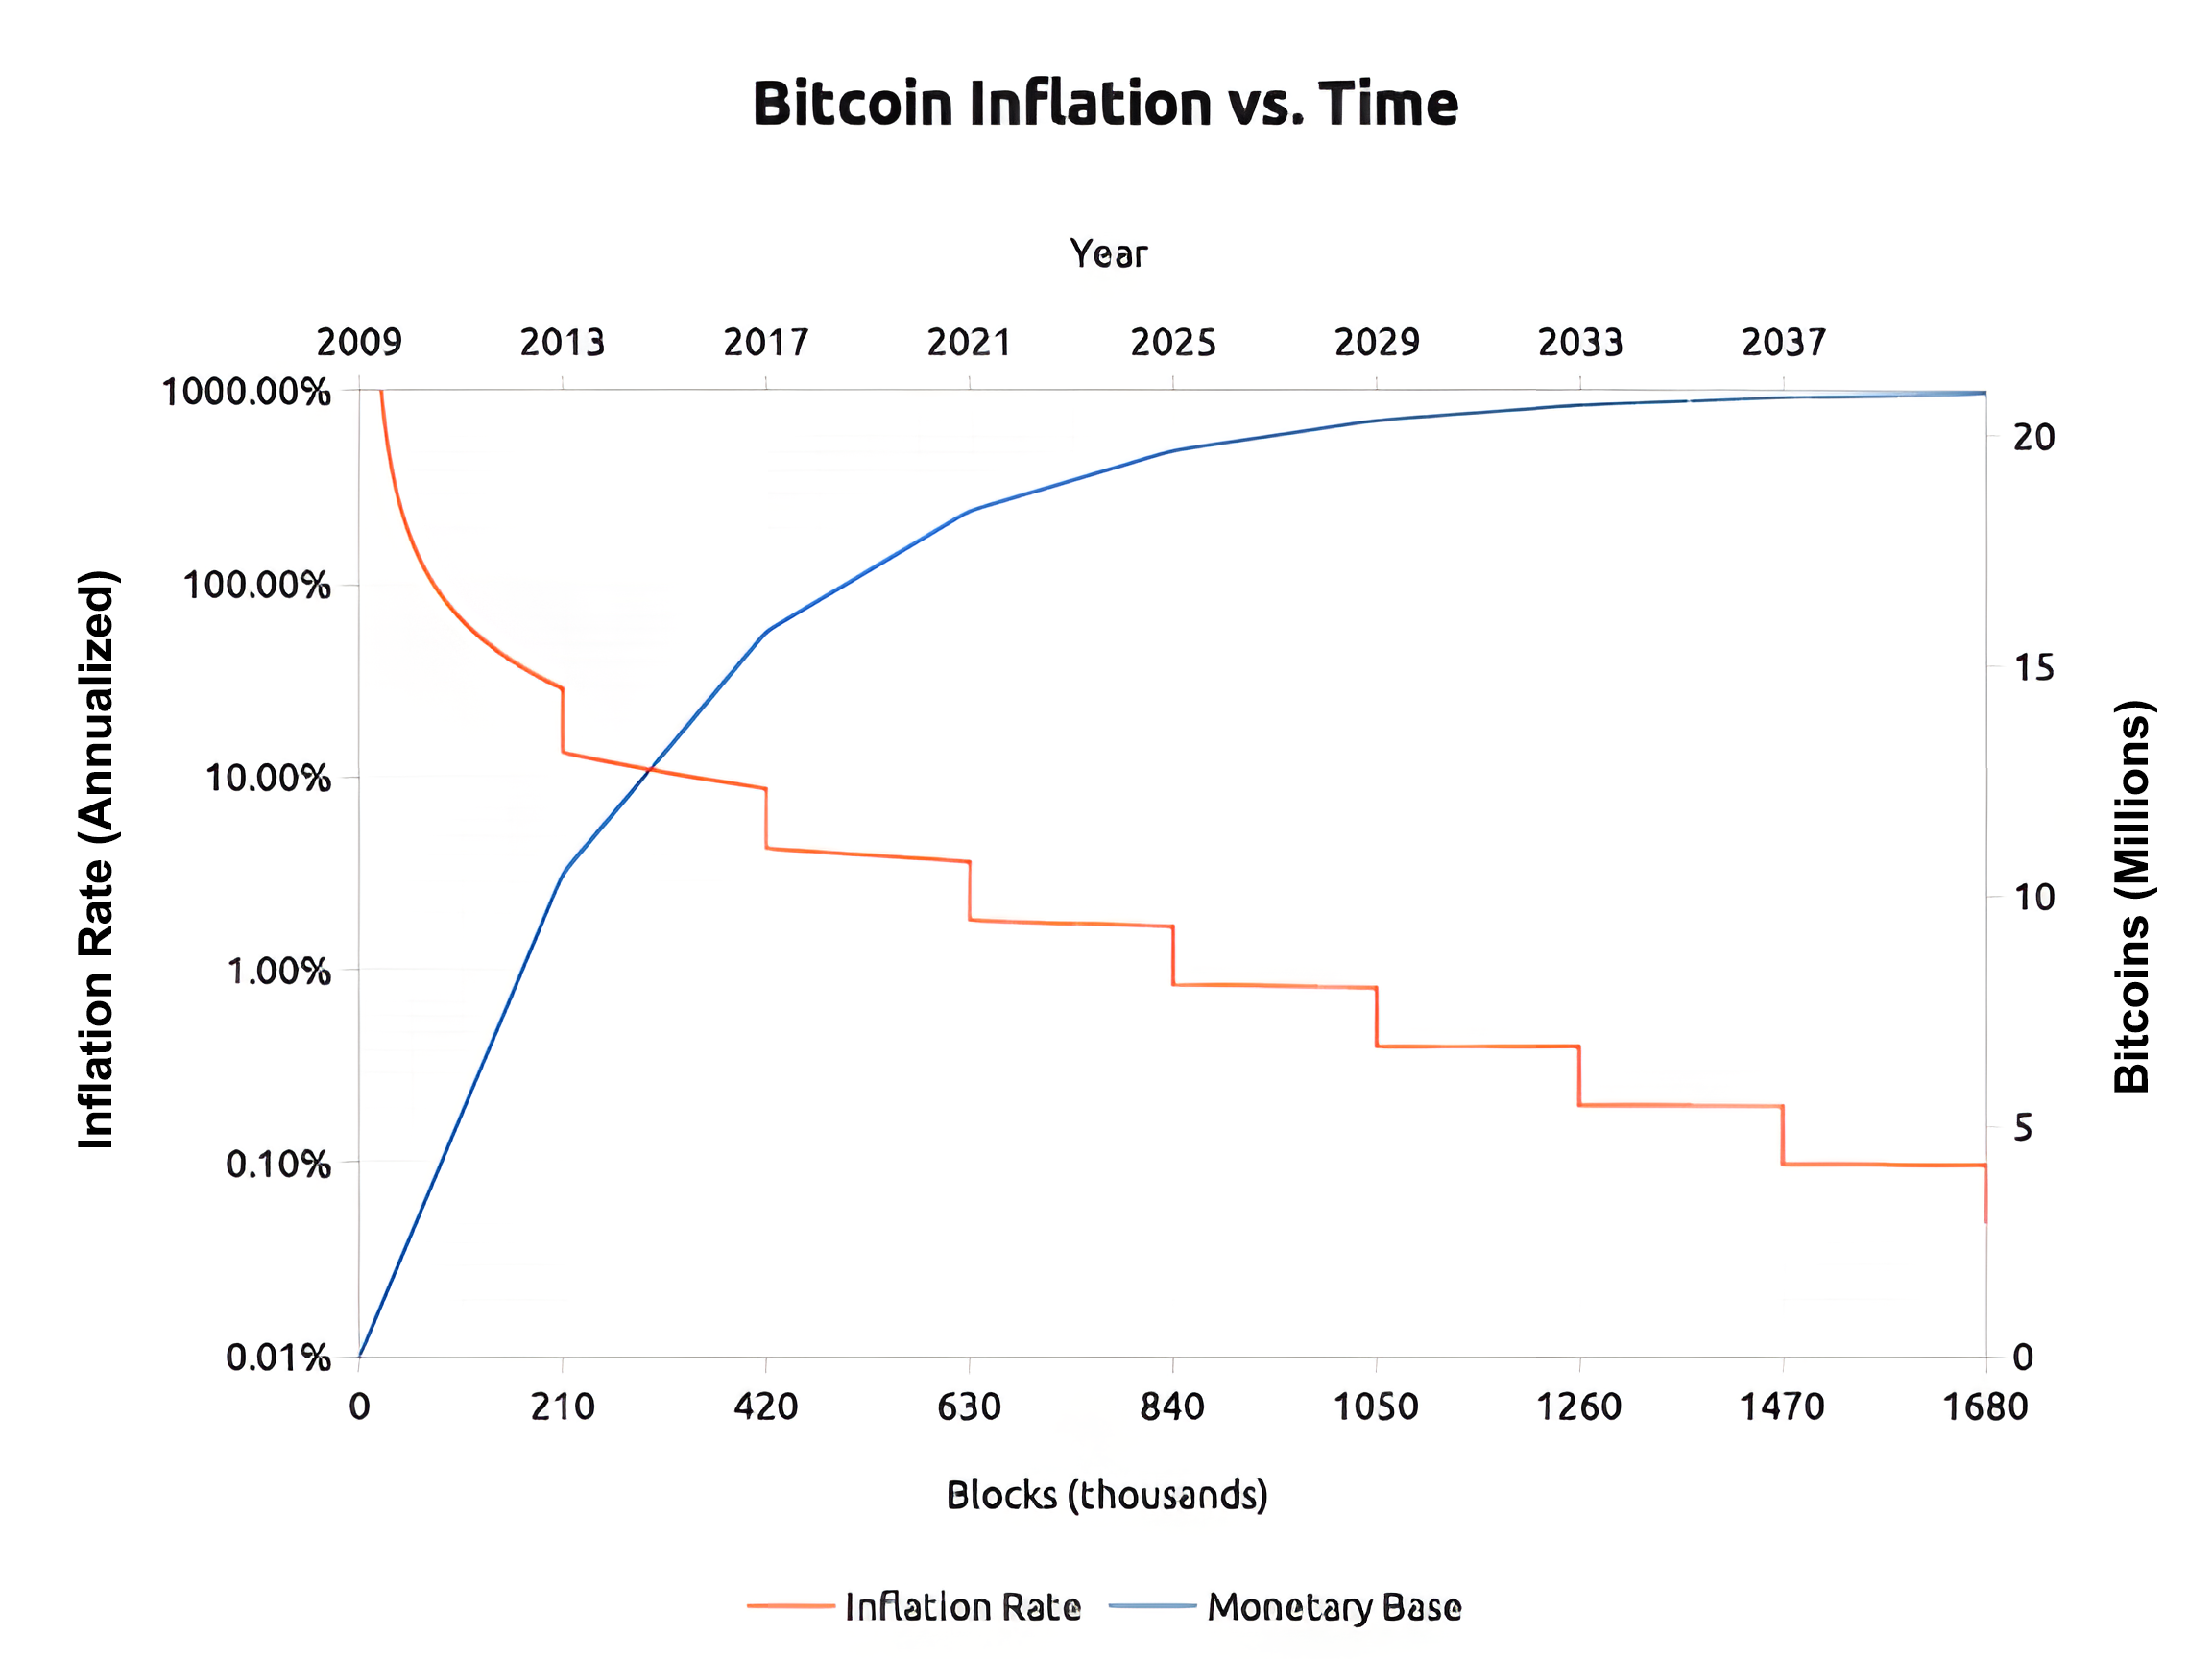
\includegraphics{chapters/img/matt-whitlock-bitcoin-inflation-log.png}

}

\caption{Matt Whitlock's graph comparing Bitcoin's emission rate and
monetary base over time (December 2012).}

\end{figure}%

The increased demand and decreased supply growth rate led to a
noticeable rise in bitcoin's price. While it hovered around \$5 during
the first part of 2012, it climbed to \$13 in August and stabilized at
that level by year's end. In 2013, its growth became exponential:
surpassing \$20 in January, it broke the previous high of \$30 in
February, and eventually reached \$266 on Mt.~Gox in April.

Symbolically, this price surge coincided with the collapse of Cypriot
banks. At that time, the financial crisis was in full swing on the
island, prompting the financial system to take drastic measures. On
March 16, 2013, banks limited customer withdrawals. On the 25th, the
Cypriot government and the EU decided (without prior legal framework)
that the Bank of Cyprus had to be internally recapitalized through a
partial tax on deposits over €100,000. The Laiki Bank, the country's
second-largest bank, was dismantled following its bankruptcy, and
holdings over €100,000 were simply confiscated. This event demonstrated
Bitcoin's utility as ``digital gold'' that can be directly owned and
isn't subject to fractional-reserve banking constraints\footnote{On this
  occasion, GoldMoney and Bitcoin Magazine co-produced a documentary
  titled \emph{Cyprus: A Wake Up Call}, collecting testimonies from
  Cypriots affected by the crisis. See on YouTube:
  \url{https://www.youtube.com/watch?v=mGGlYnxSFWM}.}.

Meanwhile, developments were also unfolding with Silk Road. The U.S.
intelligence investigation, which began in June 2011 following Adrian
Chen's Gawker article and Senators Chuck Schumer and Joe Manchin's calls
to shut down the platform, started bearing fruit. After lengthy research
and some questionable actions by investigators\footnote{Two corrupt FBI
  agents exploited the investigation to steal over 20,000 bitcoins
  (about \$350,000) and staged an assassination.---Ludovic Lars,
  ``\emph{Murders, scams, and bitcoin thefts---The dark side of Silk
  Road}'', \emph{Le Journal du Coin}, June 27, 2021:
  \url{https://journalducoin.com/analyses/cote-obscur-silk-road/}.},
Ross Ulbricht, the platform's founder, was suspected by June 2013. Gary
Alford, an IRS agent, uncovered the trail by finding Ross's initial
announcement on the Bitcoin forum and linking it to his email address,
which contained his real name. In July 2013, Silk Road's server was
seized by Icelandic police and a copy was shared with U.S. agencies. The
history contained a connection from an IP address in San Francisco, near
Ross's residence. In September, armed with this information, Ross was
identified.

Silk Road's downfall occurred in early fall 2013. On October 1, Ross
Ulbricht was apprehended by FBI agents in a San Francisco library, with
his session open on the platform. The following day, the website was
shut down, causing a stir in the community. Bitcoin's price, which had
been stabilizing around \$125 in previous days, plummeted to a low of
\$85. Between October 2 and 25, nearly 174,000 bitcoins belonging to
Ross were seized by federal agencies---a treasure worth about \$31
million at the time\footnote{29,656.52080180 BTC were sent to address
  1F1tAaz5x1HUXrCNLbtMDqcw6o5GNn4xqX between October 2 and 16, while
  144,336.39429472 BTC were transferred to address
  1FfmbHfnpaZjKFvyi1okTjJJusN455paPH on October 25.---U.S. Attorney's
  Office, Southern District of New York, \emph{Manhattan U.S. Attorney
  Announces Seizure of Additional \$28 Million Worth of Bitcoins
  Belonging to Ross William Ulbricht, Alleged Owner and Operator of
  ``Silk Road'' Website}, October 25, 2013:
  \url{https://www.justice.gov/usao-sdny/pr/manhattan-us-attorney-announces-seizure-additional-28-million-worth-bitcoins-belonging}.}.

Others associated with Silk Road were arrested and convicted in the
following years. Charlie Shrem was apprehended on January 27, 2014, by
federal agents (FBI, IRS, DEA) and charged with facilitating money
laundering through his company BitInstant. In December 2014, he was
sentenced to two years in prison for illicit transfers. Ross Ulbricht
was sentenced to two life terms plus 40 years, all for non-violent
charges, explicitly to make an example of him\footnote{During
  sentencing, Judge Katherine Forrest stated: ``I make this judgment
  mindful of the crimes you committed and the need to send the strongest
  possible message. There must be no doubt that disobedience of the law
  will not be tolerated. There must be no doubt that no one is above the
  law, no matter one's education or privileges.''---\emph{Ross
  Ulbricht's sentencing transcript}, February 4, 2015:
  \url{https://freeross.org/wp-content/uploads/2018/02/Doc_36_Jan_12_Vol_VI_Appendix_A1314-A1554.pdf\#page=240}.}.

Despite Silk Road's collapse representing the destruction of a
significant portion of Bitcoin's economy, the price rebounded, aligning
with the expectations of some major investors. Renewed enthusiasm for
Bitcoin led to another price surge and new highs. Stabilizing above
\$100, the price gradually increased in the latter half of October,
surpassing the previous high of \$266 in early November. From there, it
skyrocketed, reaching a new all-time high of \$1,240 on Mt.~Gox on
December 4, 2013. This speculative episode prompted many media outlets
to discuss Bitcoin for the first time.

However, Mt.~Gox, the epicenter of speculative activity, was more
fragile than it appeared. The platform had suffered cyberattacks
throughout its existence, leading to the gradual disappearance of funds.
By early 2014, over 650,000 bitcoins were missing from the company's
coffers, amounting to \$381 million at the time\footnote{Kim Nilsson,
  ``\emph{The missing MtGox bitcoins}'', April 19, 2015:
  \url{https://blog.wizsec.jp/2015/04/the-missing-mtgox-bitcoins.html}.}!

In February 2014, Mt.~Gox collapsed. After suspending withdrawals on the
7th, the site went offline on the 25th, and bankruptcy was declared on
the 28th. Mark Karpelès publicly apologized on Japanese television. This
crisis was catastrophic for Bitcoin: the primary hub of its economy shut
down, wealthy holders who kept their bitcoins on the platform lost
everything, and public trust (which equated Bitcoin with Mt.~Gox)
plummeted. This event ended the speculative frenzy of 2013--2014.

Mark Karpelès was suspected of embezzlement, tarnishing his reputation.
He was arrested by Japanese authorities in August 2015, earning him the
nickname ``the baron of bitcoin'' in French media. Later, it was shown
that the platform's losses resulted from multiple hacks between 2011 and
2014 and that Karpelès was only negligent and unaware of the flaw that
allowed most bitcoins to be withdrawn during that period.

Nevertheless, Mt.~Gox's downfall cleansed the exchange market. Platforms
began sharing the market more evenly, with activity distributed among
players like Bitfinex, bitFlyer, Bitstamp, Bittrex, BTCChina, BTC-e,
Coinbase, Gemini, OKEx, Kraken, and Poloniex.

\section*{The Scalability
Debate}\label{le-duxe9bat-sur-la-scalabilituxe9}
\addcontentsline{toc}{section}{The Scalability Debate}

\markright{The Scalability Debate}

The second major episode in Bitcoin's history was the scalability
debate, focusing on the system's ability to scale---that is, to continue
functioning effectively as the number of users increases. This discord
began in 2013, characterized by a sharp rise in price and activity. It
escalated into a civil war in 2015 and concluded in 2017 with a schism
into two distinct communities following the creation of a new network
called Bitcoin Cash and the cancellation of the (artificial) SegWit2X
compromise. This period was a significant learning phase for the
community. On one hand, it became aware of Bitcoin's imperfections,
which had been heralded as a decentralized digital currency system
allowing instant payments to anyone, anywhere in the world, with minimal
fees\footnote{On May 18, Bitcoin.org's homepage described Bitcoin as a
  digital currency system enabling ``instant peer-to-peer transactions
  {[}\ldots{]} worldwide'' with ``low or zero processing fees,'' noting
  that ``transaction management and bitcoin issuance are carried out
  collectively by the network.''---Bitcoin.org archive:
  \url{https://web.archive.org/web/20130518024528/http://bitcoin.org/en/}.}.
On the other hand, the community recognized the complex governance
mechanism underlying the protocol's evolution (see
chs.~\hyperref[ch:changement]{10} and \hyperref[ch:determination]{11}).

The scalability debate centered on a parameter in the protocol that
restricted the system's transactional capacity: the block size limit. In
Bitcoin, transactions are included in blocks added to the chain every 10
minutes on average; limiting block size effectively imposes a quota on
the number of confirmed transactions.

In 2013, the block size limit was 1 megabyte (1 MB), corresponding to a
theoretical maximum throughput of 7.37 transactions per second. This
limit, added to the protocol by Satoshi Nakamoto on September 12, 2010,
without public announcement, was initially meant to prevent
denial-of-service attacks and was intended to increase over
time\footnote{On October 4, 2010, Satoshi discussed on the forum how to
  implement increasing the block size limit.---Satoshi Nakamoto,
  ``\emph{Re: {[}PATCH{]} increase block size limit}'', October 4, 2010,
  19:48:40 UTC:
  \url{https://bitcointalk.org/index.php?topic=1347.msg15366\#msg15366}.}.
However, after the founder's abrupt departure, the decision was left to
community members, setting the stage for conflict.

Two main camps emerged in the debate. The first was the proponents of
larger blocks, or ``big blockers,'' who aligned themselves with
Satoshi's original vision and sought to upgrade the protocol to increase
or even remove the limit. The opposing camp consisted of proponents of
smaller blocks, or ``small blockers,'' who wanted to restrict block size
to minimize the cost of running a node.

The first vision, initially the majority, believed that progressively
increasing the block size limit could be achieved without endangering
the system's integrity. This view held that Bitcoin should remain a
payment protocol adaptable to demand without increasing transaction
fees. It favored usability over security, accepted hard forks (protocol
upgrades incompatible with previous versions requiring network-wide
coordination), and represented a more progressive stance. Its proponents
generally believed that miners determined the protocol. Developers like
Gavin Andresen, Mike Hearn, and Jeff Garzik championed this approach.

The second vision, which gained traction from 2013 onward, focused on
security at the expense of usability. Its goal was to minimize node
operation costs to maximize network decentralization. This view
considered Bitcoin primarily as a settlement protocol serving as a
foundation for layered systems, which could be centralized or
decentralized. It advocated for soft forks---backward-compatible
protocol upgrades enabled by miners, allowing gradual user adoption.
This was a more conservative position, though it acknowledged the need
for certain essential changes. Its proponents generally believed that
users upheld the protocol's integrity. Developers like Pieter Wuille,
Gregory Maxwell, Wladimir van der Laan, and Luke-Jr supported this
approach.

Within both camps, nuances and contradictions existed. The scalability
issue was complex and technical, leading to a variety of positions,
especially regarding the optimal block size limit: 1 MB, 2 MB, 8 MB?

The opposition first manifested within the Bitcoin software project,
where the lead contributors predominantly supported smaller blocks. In
spring 2014, the software underwent significant changes. Aesthetically,
it was renamed ``Bitcoin Core'' on March 19 to ``reduce confusion
between Bitcoin-the-network and Bitcoin-the-software''\footnote{Bitcoin
  Core, \emph{Bitcoin Core version 0.9.0 released}, March 19, 2014:
  \url{https://bitcoin.org/en/release/v0.9.0\#rebranding-to-bitcoin-core}.}.
Functionally, a power transition occurred on April 7 when Gavin Andresen
handed over his lead maintainer role to Wladimir van der Laan to focus
on his duties as Chief Scientist of the Bitcoin Foundation.

This management change materialized that year when Mike Hearn saw his
proposal to add the getutxos network request rejected due to lack of
unanimity within the Bitcoin Core team. Hearn needed this functionality
for his crowdfunding application, Lighthouse. Consequently, he created
Bitcoin XT in December 2014, an alternative implementation derived from
Bitcoin Core that included the desired changes while remaining
compatible with the network.

Simultaneously, the discord spread throughout the community. The small
block philosophy gained traction, notably through a video produced by
developer Peter Todd in 2013 explaining ``why the block size limit keeps
Bitcoin free and decentralized''\footnote{Keep Bitcoin Free, ``\emph{Why
  the blocksize limit keeps Bitcoin free and decentralized}'' (video),
  May 17, 2013: \url{https://www.youtube.com/watch?v=cZp7UGgBR0I}.}.
Another argument invoked was the fee market, highlighted by French
economist Nicolas Houy, who explained in a 2014 article that ``letting
transaction fees result from a market \emph{and} making block size
irrelevant or non-binding would lead to too low a security level for
Bitcoin''\footnote{Nicolas Houy, \emph{The economics of Bitcoin
  transaction fees}, GATE, 2014.---This idea, called the ``fee fatal
  spiral,'' was proposed as early as 2011 by a user on Bitcointalk. See
  Vandroiy, ``\emph{{[}If tx limit is removed{]} Disturbingly low future
  difficulty equilibrium}'', April 22, 2011:
  \url{https://bitcointalk.org/index.php?topic=6284.msg92187\#msg92187}.}.
Additionally, small block proponents sought to justify their stance by
proposing scalability solutions that would increase the economic
activity supported by the network without significantly enlarging block
size.

The first proposal was sidechains, or pegged sidechains---secondary
chains running parallel to the main chain, to and from which bitcoins
could be transferred via a two-way peg. This concept was first presented
in a technical paper on October 22, 2014, by developers from
Blockstream. Co-founded by Adam Back, Bitcoin Core developers, and
finance figures, Blockstream aimed to ``find an architecturally sound
and permissionless way to extend Bitcoin's capabilities, allowing the
cryptocurrency to reach its full potential''\footnote{Blockstream,
  \emph{Why We Founded Blockstream}, October 22, 2014, archive:
  \url{https://web.archive.org/web/20161022162335/https://www.blockstream.com/2014/10/23/why-we-are-co-founders-of-blockstream.html}.}.
Initially, it focused on developing sidechains, leading to the Elements
model and its implementation, Liquid.

The second proposal was the Lightning Network---a network of payment
channels built atop Bitcoin, enabling instant, near-free peer-to-peer
transfers. The concept was presented in February 2015 by Joseph Poon and
Thaddeus Dryja during a developer seminar in San Francisco. On February
28, they published the white paper titled ``The Bitcoin Lightning
Network,'' outlining the basics needed to build such a
network\footnote{Joseph Poon and Thaddeus Dryja, \emph{The Bitcoin
  Lightning Network DRAFT Version 0.5}, February 28, 2015:
  \url{https://lightning.network/lightning-network-paper-DRAFT-0.5.pdf}.}.
Implementing Lightning smoothly required modifying the Bitcoin protocol
by adding time locks to the scripting language and correcting a flaw
known as transaction malleability\footnote{Transaction malleability is
  the ability to slightly modify a transaction after it's broadcast on
  the network, changing its identifier. This capability disappears once
  the transaction is confirmed by a miner who includes it in a chain
  block.}.

These two proposals envisioned scaling through layering, which wouldn't
rely entirely on trusted third parties and wouldn't compromise the
entire chain's security.

Big block proponents focused on optimizing the software and protocol to
lighten node workloads. On October 6, 2014, Gavin Andresen published a
roadmap on the Bitcoin Foundation's blog describing how increased
network activity could be offset by protocol changes and exponential
technological advancements described by Moore's and Nielsen's
laws\footnote{Gavin Andresen, \emph{A Scalability Roadmap}, October 6,
  2014, archive:
  \url{https://web.archive.org/web/20150321091124/http://blog.bitcoinfoundation.org:80/a-scalability-roadmap}.}.
The article mentioned block pruning to reduce the stored chain size,
UTXO commitments to speed up initial block downloads, and block relay
via Invertible Bloom Lookup Tables for efficiency.

By spring 2015, with average block sizes approaching 500 KB, the idea of
increasing the network's transactional capacity resurfaced under Gavin
Andresen's impetus. In the following months, several proposals emerged,
including Gavin's suggestion to raise the limit to 8 MB (BIP-101),
aligning with Chinese mining pools' wishes, and Pieter Wuille's proposal
to increase the limit by 17.7\% annually (BIP-103). Unfortunately, none
of the proposals satisfied all parties, intensifying the community
conflict into a full-blown civil war.

\section*{The Block Size War}\label{la-guerre-des-blocs}
\addcontentsline{toc}{section}{The Block Size War}

\markright{The Block Size War}

The conflict over block size took a critical turn in summer 2015 with
the release of Bitcoin XT version 0.11A on August 15, which included an
increase in the block size limit---an incompatible change with network
rules\footnote{Mike Hearn, \emph{Why is Bitcoin forking?}, August 15,
  2015:
  \url{https://medium.com/faith-and-future/why-is-bitcoin-forking-d647312d22c1}.}.
The integrated upgrade was BIP-101, programming an increase of the limit
from 1 MB to 8 MB, conditional on attaining sufficient miner
signaling---specifically, 75\% of the network's hash power. As such,
this software version risked causing a network split and a chain fork
into two distinct chains.

Bitcoin XT was led by Mike Hearn, who described himself as a
``benevolent dictator'' (a common concept in the open-source world).
Gavin Andresen participated in the project and had input on its
direction, but ``Mike made the final decisions in case of severe
disputes''\footnote{\emph{FAQ---BitcoinXT} (archive):
  \url{https://web.archive.org/web/20150908031806/https://bitcoinxt.software/faq.html\#who-is-involved}.}.
Increasing the block size limit was supported by major Chinese mining
pools and some industry companies.

To a core group of the community, this movement resembled a forceful
takeover, prompting a visceral response. On the night of August 16--17,
Michael Marquardt (a.k.a. Theymos), the main moderator of the r/Bitcoin
subreddit and co-administrator of the Bitcointalk forum, published a
lengthy Reddit post announcing the banning of all discussions about
Bitcoin XT\footnote{Michael Marquardt (Theymos), ``\emph{It's time for a
  break: About the recent mess \& temporary new rules}'', August 17,
  2015, 00:50:15:
  \url{https://www.reddit.com/r/Bitcoin/comments/3h9cq4/its_time_for_a_break_about_the_recent_mess/}.}.
In it, he explained why he considered Bitcoin XT incompatible with
Bitcoin and thus undeserving of discussion on the subreddit. Since most
conversations occurred on r/Bitcoin at the time, this decision had a
significant impact.

The emergence of Bitcoin XT marked the beginning of a civil war within
the community, known as the ``block size war'' or ``Blocksize
War''\footnote{The English term comes from Jonathan Bier's book
  \emph{The Blocksize War}, published in 2021. The French term was
  coined by Morgan Phuc in 2017:
  \url{https://bitconseil.fr/bitcoin-guerre-blocs/}.}, during which
diplomacy gradually gave way to animosity. On August 17, journalist Alex
Hern wrote in \emph{The Guardian}: ``The bitcoin war has
begun''\footnote{Alex Hern, ``\emph{Bitcoin's forked: chief scientist
  launches alternative proposal for the currency}'', \emph{The
  Guardian}, August 17, 2015:
  \url{https://www.theguardian.com/technology/2015/aug/17/bitcoin-xt-alternative-cryptocurrency-chief-scientist}.}.
The period was characterized by intense propaganda from both sides,
censorship on major communication channels, and denial-of-service
attacks against nodes running Bitcoin XT and its successors.

Initially, many sought to ease the conflict and called for discussion.
This led to the ``Scaling Bitcoin'' conferences, organized to present
various ways to scale Bitcoin. The first edition took place in September
in Montreal, successfully bringing together individuals from both camps
in good faith. The second edition occurred in December in Hong Kong,
where tensions were already more palpable.

During \emph{Scaling Bitcoin II}, a new proposal for Bitcoin was
presented: Segregated Witness, or SegWit. Imagined by Gregory Maxwell
and Pieter Wuille, it aimed to facilitate Lightning Network
implementation (by correcting transaction malleability) and increase
transactional capacity in a backward-compatible way for non-mining
nodes. It was part of Gregory Maxwell's roadmap published that day on
the mailing list\footnote{Gregory Maxwell, ``\emph{{[}bitcoin-dev{]}
  Capacity increases for the Bitcoin system}'', December 7, 2015,
  22:02:17 UTC:
  \url{https://lists.linuxfoundation.org/pipermail/bitcoin-dev/2015-December/011865.html}.}
and quickly became the upgrade championed by small block proponents.

At the beginning of 2016, Bitcoin XT failed, and Mike Hearn left the
community in a high-profile resignation\footnote{Mike Hearn, \emph{The
  resolution of the Bitcoin experiment}, January 14, 2016:
  \url{https://blog.plan99.net/the-resolution-of-the-bitcoin-experiment-dabb30201f7}.}.
However, a new implementation emerged among big block supporters:
Bitcoin Classic. It incorporated a modified version of BIP-101,
proposing a 2 MB block size limit upon reaching 75\% network hash power
signaling. Bitcoin Classic quickly gained popularity, prompting concern
from the opposing camp\footnote{``Bitcoin Classic emerged from the ashes
  of the XT vs.~Core debate. It's a version of Bitcoin that would allow
  a two-megabyte limit, setting rules to increase it over time. It seems
  to be rapidly gaining support.''---Paul Vigna, ``\emph{Is Bitcoin
  Breaking Up?}'', \emph{The Wall Street Journal}, January 17, 2016,
  archive:
  \url{https://web.archive.org/web/20160117220315/https://www.wsj.com/articles/is-bitcoin-breaking-up-1453044493}.}.

On February 20, 2016, an emergency meeting was held in Hong Kong. This
``roundtable'' brought together major mining pools, some ecosystem
companies, and key Bitcoin Core contributors like Matt Corallo, Peter
Todd, and Luke-Jr.~After hours of pressured discussions, participants
reached an agreement, later known as the Hong Kong Agreement. Developers
agreed to implement SegWit and double the base block size limit, while
miners committed to activating SegWit and using only Bitcoin
Core\footnote{Bitcoin Roundtable, \emph{Bitcoin Roundtable Consensus},
  February 20, 2016:
  \url{https://medium.com/@bitcoinroundtable/bitcoin-roundtable-consensus-266d475a61ff}.}.

However, this sense of compromise didn't last, as two events in 2016
changed the dynamics. The first was the involvement of Craig S. Wright,
an Australian computer scientist and entrepreneur who claimed to be
Satoshi Nakamoto. He was thrust into the spotlight in December 2015
following independent investigations by \emph{Wired} and \emph{Gizmodo},
which suggested he might be Bitcoin's creator. The investigations were
based on evidence indicating he might have been involved in
cryptocurrency development alongside his friend Dave Kleiman, who died
in 2013.

A few months later, on May 2, 2016, Craig Wright published a lengthy and
convoluted blog post\footnote{Craig Wright, \emph{Jean-Paul Sartre,
  Signing and Significance}, May 2, 2016, archive:
  \url{https://web.archive.org/web/20160502072011/http://www.drcraigwright.net/jean-paul-sartre-signing-significance/}.},
including a signature corresponding to the public key used to receive
the block 9 reward and send the first payment to Hal Finney in January
2009. Additionally, a BBC interview with Wright was released that day,
in which he claimed to have been the ``main part'' of Satoshi Nakamoto
but that ``other people helped {[}him{]}''\footnote{BBC News, \emph{Mr
  Bitcoin: ``I don't want money, I don't want fame!''} (video), May 2,
  2016: \url{https://www.youtube.com/watch?v=5DCAC1j2HTY}.}. He also
claimed to have signed a message privately in front of the interviewing
journalist.

However, it quickly became apparent that the documents provided in the
investigations and the elements presented by Wright himself were
unconvincing. Specifically, the signature in the blog post was
discovered to be the signature of an existing transaction on the Bitcoin
blockchain, simply encoded differently\footnote{The signature provided
  by Craig Wright corresponds to the public key linked to address
  12cbQLTFMXRnSzktFkuoG3eHoMeFtpTu3S, which received the block 9 reward
  and sent the first payment to Hal Finney on January 12, 2009, and was
  thus produced by Satoshi Nakamoto. A Reddit user (JoukeH) quickly
  discovered it was the signature of an existing transaction on the
  chain:
  \url{https://www.reddit.com/r/Bitcoin/comments/4hf4xj/creator_of_bitcoin_reveals_identity/d2pf70v/}.}.
This fact prompted caution within the community.

That same day, Gavin Andresen published an article stating he believed
Craig Wright was ``the person who invented Bitcoin,'' as Wright had
shown him ``messages signed with keys only Satoshi should possess'' in
person\footnote{Gavin Andresen, \emph{Satoshi}, May 2, 2016:
  \url{http://gavinandresen.ninja/satoshi}}. Consequently, Gavin's
maintainer role and commit access to the Bitcoin Core repository were
revoked immediately, ostensibly because the team feared his account had
been hacked. Overall, this dubious assertion, confirmed in person at the
Consensus 2016 conference, discredited him, and his GitHub access was
never restored. He later acknowledged being deceived.

The second event influencing the conflict didn't occur within the
Bitcoin community but on Ethereum, an alternative system launched in
2015 dedicated to smart contracts. It was the split between Ethereum
(ETH) and Ethereum Classic (ETC) following TheDAO hack.

On June 17, 2016, TheDAO---a decentralized autonomous organization aimed
at investing in the ecosystem---was hacked, and 3.6 million ethers
(Ethereum's unit of account) worth \$50 million were stolen,
representing 4.4\% of the total ether supply at the time. The community
decided by a large majority to simply reverse the theft by altering the
system's state. A month later, on July 20, the change was implemented,
leading to a chain split: one following the modified protocol (which
became the majority and retained the name Ethereum) and one following
the original protocol (which became the minority and was called Ethereum
Classic). Holders ended up with different ethers on both sides.

This split wasn't clean. Notably, it didn't include replay protection,
meaning transactions made on one chain could be replicated on the other
by a third party, leading to replay attacks. This disrupted exchanges
that had to contend with the issue. Consequently, although the combined
price of both ethers eventually surpassed the initial ether's price,
everyone could observe the negative effects of a hard fork-induced
split. This example reinforced small block proponents' conservative
stance advocating for protocol evolution through soft forks like SegWit.

Due to these events, the big block camp emerged from 2016 significantly
weakened, both reputation-wise and in terms of arguments.

It was at this point that Bitcoin Core developers initiated miner
signaling for SegWit, starting November 15, 2016, for a one-year period.
The upgrade required 95\% hash power signaling to activate, aiming to
ensure widespread backward compatibility.

However, major mining pools refused SegWit (for various
reasons\footnote{SegWit notably nullified the effects of the secret
  AsicBoost, a mining optimization technique. See Gregory Maxwell,
  ``\emph{{[}bitcoin-dev{]} BIP proposal: Inhibiting a covert attack on
  the Bitcoin POW function}'', April 5, 2017, 21:37:45 UTC:
  \url{https://lists.linuxfoundation.org/pipermail/bitcoin-dev/2017-April/013996.html}.}),
and during the initial months, the proportion of blocks signaling
support stagnated around 25\%, far from the required threshold. SegWit
was stalled.

At the beginning of 2017, blocks began to fill up, leading to a
significant increase in transaction fees and confirmation times on the
chain. By mid-February, median fees exceeded 30 cents for the first time
in Bitcoin's history. In this context, pressure for change grew on both
sides.

One side rallied around Bitcoin Unlimited, an implementation that gained
popularity among big block supporters during summer 2016, succeeding
Bitcoin Classic. It was notably backed by Roger Ver, CEO of Bitcoin.com,
who had become an influential community figure\footnote{Roger Ver is
  known for promoting bitcoin adoption among merchants and his prominent
  role in the documentary \emph{The Bitcoin Gospel}, released on
  November 1, 2015, on YouTube. See
  \url{https://www.youtube.com/watch?v=8zKuoqZLyKg&t=2831s}.}, providing
substantial funding for Bitcoin Unlimited. By March 2017, signaling for
Unlimited surpassed that of SegWit.

However, on March 17, the possibility of a contentious hard fork
prompted exchanges to consider the potential currency created by Bitcoin
Unlimited as an alternative cryptocurrency. Drawing on their experience
with the ETH and ETC split, they demanded that it include replay
protection; otherwise, it wouldn't even be listed. This decision was
devastating for big block proponents.

On the other side, pressure to activate SegWit intensified among small
block supporters, who were growing impatient. On March 12, 2017, an
individual known as Shaolin Fry published a proposal for a User
Activated Soft Fork (UASF) that would lock in the upgrade without miner
signaling by August 1\footnote{Shaolin Fry, ``\emph{{[}bitcoin-dev{]}
  Flag day activation of segwit}'', March 12, 2017, 15:50:27 UTC:
  \url{https://lists.linuxfoundation.org/pipermail/bitcoin-dev/2017-March/013714.html}.}.
This bold measure was dangerous and didn't gain unanimous support among
small blockers, as illustrated by Gregory Maxwell's opposition.

However, the UASF threat existed and exerted influence. Faced with the
community's desire for SegWit, major ecosystem players (companies and
miners) were compelled to sign an agreement on May 23, 2017, on the
sidelines of the Consensus 2017 conference in New York. This New York
Agreement, as it became known, represented a theoretical compromise in
the raging conflict: signatories committed to activating SegWit with an
80\% hash power threshold and doubling the block size limit within six
months. The implementation embodying this agreement was called SegWit2X.
This pseudo-compromise was quickly criticized due to the absence of
Bitcoin Core developers at the meeting---they simply weren't invited.

The agreement led to SegWit's activation during summer 2017. In July,
miners began massively signaling support. On the 21st, the lock-in
process was initiated (rendering the UASF ineffective). SegWit was
finally activated on August 24, 2017.

The upgrade proceeded smoothly. However, at the same time, another split
occurred---this time, fully intentional. In opposition to the UASF,
miners decided to activate a new protocol incompatible with the
original, which didn't include SegWit and implemented an 8 MB block size
limit: Bitcoin Cash. The protocol's launch was overseen by Amaury
Séchet, a French developer.

On August 1, 2017, with block 478,559 mined at 6:12 PM, Bitcoin Cash was
born. Following this split, bitcoin holders ended up with equivalent
amounts in bitcoins (BTC) and bitcoin cash (BCH). Those who disapproved
of SegWit joined Bitcoin Cash.

In August, as SegWit was finally locked in, some small block proponents
began opposing the second part of SegWit2X---the doubling of block
size---through a communication campaign dubbed ``NO2X.'' Their argument
emphasized the lack of replay protection in this hard fork. SegWit2X was
designed as a non-contentious change and therefore didn't include such
measures, which would have significantly burdened the upgrade process
for wallets.

Opposition grew. Bitcoin Core developers refused to endorse the change.
Users mobilized to protest, arguing that ``the way the agreement was
reached goes against Bitcoin's very essence''\footnote{``We oppose the
  New York Agreement and the November Bitcoin SegWit2X hard fork,''
  Change.org, October 15, 2017:
  \url{https://www.change.org/p/mineurs-et-entreprises-de-l-éco-système-bitcoin-nous-nous-opposons-au-new-york-agreement-et-au-hard-fork-bitcoin-segwit2x-de-novembre}.}.
Faced with this resistance, the companies signing the New York Agreement
gradually withdrew.

The plan to double the block size limit was ultimately abandoned on
November 8, 2017, a week before its scheduled activation. The project's
promoters---Mike Belshe, Wences Casares, Jihan Wu, Jeff Garzik, Peter
Smith, and Erik Voorhees---jointly stated:

``Our goal has always been a smooth upgrade for Bitcoin. While we
strongly believe in the need for a larger block size, there is something
we believe is even more important: keeping the community together.
Unfortunately, it is clear that we have not built sufficient consensus
for a clean block size upgrade at this time. Continuing on the current
path could divide the community and be a setback for Bitcoin's growth.
This was never the goal of Segwit2x''\footnote{Mike Belshe,
  ``\emph{{[}Bitcoin-segwit2x{]} Segwit2x Final Steps}'', November 8,
  2017, 16:58:41 UTC:
  \url{https://lists.linuxfoundation.org/pipermail/bitcoin-segwit2x/2017-November/000685.html}.}.

This was a significant victory for the small block philosophy, which
would henceforth dominate the chain. As for scalability solutions on
BTC, the Lightning Network was launched in beta in March 2018. The
sidechain concept was also experimented with, with the launch of
Rootstock in January 2018 and Blockstream's Liquid sidechain in
September that same year.

On the other side, following SegWit2X's cancellation, many proponents of
increased chain capacity turned to other protocols like Bitcoin Cash or
Ethereum.

Despite constant denigration from detractors, Bitcoin Cash's evolution
continued. However, its community gradually fragmented, leading to two
major splits: the creation of Bitcoin SV in November 2018 and ``eCash''
(XEC) in November 2020. The market share of the entire group plummeted
accordingly: by November 2023, the combined value of these three
cryptocurrencies represented less than 1\% of BTC's value.

\section*{The Rise of Alternative
Cryptocurrencies}\label{lessor-des-cryptomonnaies-alternatives}
\addcontentsline{toc}{section}{The Rise of Alternative Cryptocurrencies}

\markright{The Rise of Alternative Cryptocurrencies}

Bitcoin is a free project based on open-source code that anyone can copy
and deploy on a new network. This characteristic is excellent for
innovation: anyone can modify the code and use it as the foundation for
a new cryptocurrency. Bitcoin's discovery thus opened the door to
genuine currency competition on the Internet. However, this freedom also
exists for ill-intentioned individuals who can exploit this openness to
create dubious projects---from useless cryptocurrencies to outright
scams, including open Ponzi schemes. The rise of ``alternative
cryptocurrencies'' (or ``altcoins'') emerged from this duality between
the honest innovator and the greedy wrongdoer.

The first idea of a cryptocurrency distinct from Bitcoin appeared while
Satoshi was still active in the community. In November 2010, a
discussion about a distributed domain name system (then called BitDNS)
began on IRC and the Bitcoin forum. The idea was to associate website
identifiers (DNS) with coins created by the protocol, similar to
bitcoins in Bitcoin. Because the registry would be public and
tamper-resistant, it would improve upon the existing system. Satoshi
wasn't opposed and suggested merged mining with Bitcoin's
chain\footnote{Satoshi Nakamoto, ``\emph{Re: BitDNS and Generalizing
  Bitcoin}'', December 9, 2010, 21:02:42 UTC:
  \url{https://bitcointalk.org/index.php?topic=1790.msg28696\#msg28696}.}.
This led to the creation of Namecoin in April 2011, initiated by Vincent
Durham.

Subsequently, other cryptocurrencies emerged, such as Ixcoin and
Tenebrix. Tenebrix was notable for implementing the scrypt proof-of-work
algorithm, developed by miner ArtForz and supposedly resistant to GPUs.
In October 2011, Litecoin was launched by Charlie Lee as a ``lite
version of Bitcoin,'' with blocks mined four times faster, units four
times less scarce, and incorporating the scrypt algorithm. Litecoin
aimed to be ``silver to Bitcoin's gold''\footnote{Charlie Lee (coblee),
  ``\emph{Re: {[}ANN{]} Litecoin---a lite version of Bitcoin. Be ready
  when it launches!}'', October 9, 2011, 06:14:28 UTC:
  \url{https://bitcointalk.org/index.php?topic=47417.msg564414\#msg564414}.}.

In August 2012, Sunny King and Scott Nadal launched PPCoin, a system
introducing the proof-of-stake mechanism, presented as an
energy-efficient alternative to proof-of-work in the long
term\footnote{Sunny King, ``\emph{{[}ANN{]} {[}PPC{]} PPCoin
  Released!---First Long-Term Energy-Efficient Crypto-Currency}'',
  August 19, 2012, 19:54:28 UTC:
  \url{https://bitcointalk.org/index.php?topic=101820.msg1113938\#msg1113938};
  Sunny King, Scott Nadal, ``\emph{PPCoin: Peer-to-Peer Crypto-Currency
  with Proof-of-Stake}'', August 19, 2012, archive:
  \url{https://web.archive.org/web/20121021014644/http://www.ppcoin.org/static/ppcoin-paper.pdf}.}.
Proof-of-stake was integrated in a hybrid manner alongside
proof-of-work. PPCoin gradually became known as Peercoin over the years.

In 2013, with the financial enthusiasm resulting from bitcoin's success,
creating original cryptocurrencies became extremely profitable. New
protocols multiplied, such as Feathercoin in April, Primecoin in July,
and the famous Dogecoin in December. Coinmarketcap.com was launched in
May 2013 to list cryptocurrencies and rank them by ``market
capitalization''---that is, their aggregate value (number of units
multiplied by unit price).

However, not everyone appreciated this proliferation, and a movement of
rejection formed against what seemed like a harmful fragmentation of the
ecosystem. As early as 2011, skepticism towards the first alternative
cryptocurrencies was evident, as seen in Hal Finney's and Gavin
Andresen's reactions. The rejection became more pronounced in August
2013 with Gavin Andresen equating the creation of new cryptocurrencies
to inflation\footnote{Gavin Andresen, \emph{The macro-economics of
  alt-coins}, August 19, 2013:
  \url{https://gavintech.blogspot.com/2013/08/the-macro-economics-of-alt-coins.html}.},
and Daniel Krawisz, a writer for the Satoshi Nakamoto Institute,
highlighting the extreme difficulty of surpassing Bitcoin's network
effect\footnote{Daniel Krawisz, \emph{The Problem with Altcoins}, August
  22, 2013:
  \url{https://nakamotoinstitute.org/mempool/the-problem-with-altcoins/}.}.

In parallel, a contrary trend emerged: cryptomonetary pluralism
advocating openness and tolerance towards cryptocurrency diversity. This
was notably defended by the young Vitalik Buterin in September
2013\footnote{Vitalik Buterin, ``\emph{In Defense of Alternative
  Cryptocurrencies}'', \emph{Bitcoin Magazine}, September 7, 2013:
  \url{https://bitcoinmagazine.com/business/defense-alternative-cryptocurrencies}.},
who put it into practice by developing his own project, Ethereum.

From 2014 onward, this trend was reinforced by the emergence of
fundamentally more relevant crypto-economic systems than mere Bitcoin
copies. To address Bitcoin's lack of privacy, several solutions emerged.
Darkcoin, launched in January 2014 (later becoming Dash), was one such
example. Monero, a protocol integrating default privacy whose name means
``coin'' in Esperanto, was launched in April. Additionally, the
publication of the Zerocoin and Zerocash protocols by Matthew Green in
2013 led to the creation of Zcash in October 2016.

But privacy wasn't the only area of innovation. Other separate protocols
emerged to implement enhancements to Bitcoin's programmability, aligning
with the idea of a ``Bitcoin 2.0'' spreading within the community.
Indeed, Satoshi's protocol was ill-suited for complex operations and
creating secondary digital tokens, even though this was possible on
layers like Omni and Counterparty. Thus, new systems appeared, such as
Bitshares---a decentralized marketplace notable for its delegated
proof-of-stake mechanism---and NXT, a platform featuring a wide range of
functionalities. However, the standout system was Ethereum.

Ethereum generalized Bitcoin's programmability by creating a kind of
decentralized world computer operating in parallel on all nodes of a
peer-to-peer network. The project originated from Vitalik Buterin's
vision at the end of 2013. Along with seven co-founders, he conducted a
token pre-sale in July--August 2014, raising 31,529 bitcoins\footnote{The
  BTC address used by EthSuisse was
  36PrZ1KHYMpqSyAQXSG8VwbUiq2EogxLo2.---Vitalik Buterin, \emph{Launching
  the Ether Sale}, July 22, 2014:
  \url{https://blog.ethereum.org/2014/07/22/launching-the-ether-sale}.}
(over \$15 million at the time) to fund development. Ethereum was
intentionally more progressive, innovative, and flexible than Bitcoin.
The chain was officially launched a year later, on July 30, 2015.

In 2014, the first stablecoin also appeared: Tether USD (USDT), launched
on the Bitcoin chain on October 6 under the name Realcoin. This digital
token was pegged to the dollar through the guarantee of Tether Limited,
which committed to redeem each unit for a real dollar. This ``stable''
cryptocurrency allowed individuals and exchanges to benefit from the
dollar's low volatility without facing legal inconveniences.

In response to this development, the movement rejecting these new
projects continued to grow. It was exemplified on October 22, 2014, by
Blockstream's sidechain paper, describing how Bitcoin could serve as the
foundation for all use cases, and a complementary article explaining the
rationale behind the company's founding. In the latter, Blockstream
developers wrote:

``The altcoin approach of creating a new cryptocurrency solely to
introduce new features creates uncertainty for those observing
cryptocurrencies from the outside. There seems to be no natural stopping
point, with each copy being potentially copied again, ad infinitum. This
creates both market fragmentation and development fragmentation. We
believe that for cryptocurrencies to succeed as a whole, we must foster
network effect, not fragmentation''\footnote{Blockstream, \emph{Why We
  Founded Blockstream}, October 22, 2014, archive:
  \url{https://web.archive.org/web/20161022162335/https://www.blockstream.com/2014/10/23/why-we-are-co-founders-of-blockstream.html}.}.

Over the years, this rejection gradually became known as Bitcoin
maximalism, reappropriating the term used pejoratively by Vitalik
Buterin against those who systematically disparaged alternative
cryptocurrencies\footnote{The expression used by Vitalik Buterin was
  ``bitcoin dominance maximalist''
  (\url{https://www.reddit.com/r/Bitcoin/comments/2is4us/whats_wrong_with_counterparty/cl54c0y/}).
  In his article published on November 19, 2014, he defined Bitcoin
  maximalism as ``the idea that a multi-currency universe is
  undesirable, that launching `yet another coin' is morally wrong, and
  that it is both just and inevitable that the Bitcoin currency comes to
  take a monopoly position in the cryptocurrency scene.''---Vitalik
  Buterin, \emph{On Bitcoin Maximalism, and Currency and Platform
  Network Effects}, November 19, 2014:
  \url{https://blog.ethereum.org/2014/11/20/bitcoin-maximalism-currency-platform-network-effects/}.}.
The movement advocated maximizing Bitcoin's economic dominance over
close competitors and prescribed its adherents to act accordingly. The
aim was to emphasize network effect, not only because it was technically
necessary but also because it was morally desirable\footnote{Membership
  in maximalism is sometimes claimed today by people who don't embrace
  its extremist nature (even if it's inherent in the term). That's why
  the pleonasm ``toxic maximalism'' can be used to describe this
  tendency. Jameson Lopp also refers to ``bitcoin puritanism.'' See
  Jameson Lopp, \emph{History of Bitcoin Maximalism}, March 25, 2023:
  \url{https://blog.lopp.net/history-of-bitcoin-maximalism/}.}.

However, faced with Bitcoin's limitations highlighted during the block
size war, the phenomenon of substitution by other crypto-economic
systems intensified over time. From March 2017, BTC's dominance over
other cryptocurrencies dropped from around 85\%, where it had held
steady, to 40\% by June. This was partly due to Ethereum's rise, which
provided a simple way to issue programmable tokens on its blockchain.
This functionality enabled fundraising through token pre-sales, known as
Initial Coin Offerings (ICOs), to finance projects involving the tokens.
The number of such fundraisers exploded in 2017--2018, leading to the
so-called ``ICO craze.'' The largest, EOS, raised \$4.1 billion over a
year.

In 2019, another enthusiasm emerged: decentralized finance, or DeFi.
DeFi aimed to replicate traditional financial system tools in a digital,
decentralized, open, and transparent manner. The goal was to minimize
intermediation (often imperfectly) in executing various financial
operations: exchanges, secured lending, derivatives creation, predictive
markets, and so on. This development mainly occurred on Ethereum and was
embodied by the rise of the Maker protocol, enabling the existence of
the first decentralized stablecoin---the dai. In DeFi, BTC was used as
prime collateral. Alongside this, a new trend around non-fungible tokens
(NFTs) emerged, gaining mainstream attention from 2021.

However, all these projects suffered from significant technical and
human flaws, making criticism still relevant. Many lacked the
``decentralization'' they claimed. Others were duplicates offering
nothing new and disappeared due to the network effect of competitors.
Others were outright scams, with promoters lying to sell their tokens.
This explains why Bitcoin maximalism persists at the time of writing.

\section*{Institutional
Integration}\label{lintuxe9gration-institutionnelle}
\addcontentsline{toc}{section}{Institutional Integration}

\markright{Institutional Integration}

The openness to traditional finance initiated in 2012 gradually
translated into integration within the existing legal system. This trend
was natural: for Bitcoin to exist, it needed a certain level of
tolerance from the public and, ultimately, from authorities that
``represent'' them.

Institutionalization began primarily through regulation---subjecting the
sector to a legal framework generally defined and enforced by the state.
In practice, this meant subjecting significant financial players to more
or less stringent standards. Regulation thus equated to
control---something fundamentally opposed by Bitcoin, leading to
inherent tension.

From Bitcoin's early years, intelligence agencies took an interest, both
in the U.S. and France. In April 2011, the CIA invited Gavin Andresen to
discuss Bitcoin, which he did in June. On May 9, 2012, an internal FBI
report on Bitcoin leaked online, stating that ``if Bitcoin stabilizes
and grows in popularity, it will become an increasingly useful tool for
various illegal activities beyond the cyber realm''\footnote{Kim Zetter,
  ``\emph{FBI Fears Bitcoin's Popularity with Criminals}'',
  \emph{Wired}, May 9, 2012:
  \url{http://www.wired.com/2012/05/fbi-fears-bitcoin/}.}. In July 2012,
a Tracfin report noted that ``virtual currencies'' posed a ``specific
risk in terms of combating money laundering and terrorist
financing''\footnote{Tracfin, \emph{2011 Activity Report}, July 2012:
  \url{https://www.economie.gouv.fr/files/files/directions_services/tracfin/Publications/rapports_activite/2011_rapport_FR.pdf}}.

These investigations paved the way for financial regulations starting in
2013, spurred by the spring price surge. On March 18, FinCEN (Financial
Crimes Enforcement Network) published a document clarifying its position
on digital currencies\footnote{Financial Crimes Enforcement Network,
  \emph{Application of FinCEN's Regulations to Persons Administering,
  Exchanging, or Using Virtual Currencies}, March 18, 2013:
  \url{https://www.fincen.gov/sites/default/files/shared/FIN-2013-G001.pdf}.},
specifying that exchanges were Money Services Businesses (MSBs) and thus
required licenses to operate in the U.S.

Gradually, standards tightened. Exchanges began implementing Know Your
Customer (KYC) procedures by requiring identity verification to access
their services. They could also go further under Anti-Money Laundering
and Countering the Financing of Terrorism (AML/CFT) regulations.

Other financial regulations applied to cryptocurrencies, such as capital
gains taxation. In France, for example, users are legally required to
declare capital gains from the ``sale of digital assets for valuable
consideration'' and pay a 30\% tax if total sales exceed €305
annually\footnote{French General Tax Code, \emph{Article 150 VH bis},
  May 24, 2019.}.

Regulations differed between jurisdictions. While some were lenient,
others were much stricter. For example, New York State enacted
ultra-restrictive regulations in 2015, requiring many ecosystem players
to obtain a ``BitLicense.'' Similarly, France issued a decree in
November 2019 subjecting Digital Asset Service Providers (DASPs) to
stringent conditions. In both cases, local actors fled to more
accommodating jurisdictions.

Beyond regulation, traditional players' discourse was initially openly
hostile to Bitcoin's original conception. This was evident in 2014--2015
with the emergence of the term ``blockchain technology,'' aiming to deny
the rebellious aspect of the cryptocurrency by amalgamating all
distributed consensus techniques under one label. The call for
blockchain was popularized in 2015 by Blythe Masters, a former JPMorgan
Chase trader known for creating credit default swaps (CDS), which were
at the root of the subprime mortgage crisis\footnote{Edward Robinson,
  Matthew Leising, ``\emph{Blythe Masters Tells Banks the Blockchain
  Changes Everything}'', \emph{Bloomberg}, September 1, 2015:
  \url{https://www.bloomberg.com/news/features/2015-09-01/blythe-masters-tells-banks-the-blockchain-changes-everything}.}.
However, over time, the discourse softened.

Regulation introduced new constraints, in direct opposition to Bitcoin's
intrinsic permissionless nature. But it gradually allowed larger
investors, like investment funds, to enter the market with liquidity,
legitimizing the cryptocurrency in the eyes of the general public, who
often required official approval to take interest. This prompted some
community members to seek cooperation with regulators.

In 2017, a new speculative frenzy emerged, with bitcoin's price sharply
rising from \$1,000 in January to \$20,000 in December. This new bubble
again attracted media attention. Bitcoin was now taken much more
seriously. In December 2017, it even entered the Chicago Mercantile
Exchange through futures contracts---a notable advancement.

After the block size war, BTC was increasingly seen strictly as digital
gold---an asset uncorrelated with other financial markets that could
serve as a safe haven. Some analysts even began considering
crypto-assets as a new asset class. For a growing number of users,
bitcoin was perceived as a store of value that could serve as a
benchmark for the global monetary system and integrate into the legal
systems of various state entities.

This shift in perception caused a growing conflict between those who
viewed bitcoin as an intermediary for black-market transactions and
those who saw it as a reserve currency. One side, proponents of
Bitcoin's free and permissionless aspect, categorically rejected any
regulation, viewing it as compromising the project's original values.
The other side, proponents of the reserve currency concept, realized
that cooperating with authorities was necessary for the wealthiest
entities (investment funds, large companies, states) to buy in. To
achieve this, they bet on interest representation (lobbying) and
geopolitical context (diplomacy).

In 2020, the global response to the COVID-19 pandemic accelerated
developments. Western states imposed strict lockdowns, paralyzing their
economies and triggering the start of a deflationary crisis. Central
banks reacted accordingly by injecting record liquidity. As in 2008, the
goal was to save the economy by creating money and injecting it into the
market: \$2.3 trillion were issued in the U.S. and €1.85 trillion in the
European Union\footnote{In the U.S., the Coronavirus Aid, Relief, and
  Economic Security Act (CARES Act), signed in March 2020, accounted for
  this additional expenditure. It was a Treasury Department program, but
  we can assume it was primarily funded by ``borrowing'' from the
  Federal Reserve. On the European Central Bank side, liquidity
  injections were implemented through the Pandemic Emergency Purchase
  Programme (PEPP), which planned €750 billion in March 2020, plus €600
  billion in June, and an additional €500 billion in December.}.
Additionally, key interest rates were lowered to near zero to stimulate
lending, further increasing the available scriptural money supply.

Due to this massive monetary creation, the threat of high inflation
reappeared in the West, having been absent for decades. This risk
prompted people to buy bitcoin, which, as an asset independent of
monetary creation, made perfect sense. Notably, large publicly traded
U.S. companies with significant dollar reserves joined in. On August 11,
2020, MicroStrategy, led by Michael Saylor, announced adopting bitcoin
as its primary reserve asset, acquiring 21,454 BTC for a total purchase
price of \$250 million. In October, Square---an American mobile payment
company co-founded by Jack Dorsey---followed suit, acquiring 4,709
bitcoins. In February 2021, electric car maker Tesla, led by Elon Musk,
announced purchasing nearly 43,000 BTC for \$1.5 billion.

Consequently, a new speculative surge occurred, and bitcoin's price
soared again. Hovering around \$10,000 since 2019, it rose rapidly in
fall 2020, surpassing its previous high in December and reaching
\$64,000 in April 2021.

\begin{figure}

{\centering 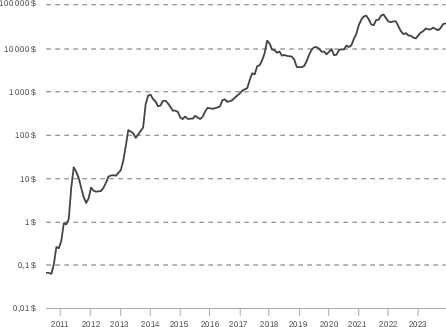
\includegraphics{chapters/img/btc-historical-price-20100719-20231130.png}

}

\caption{BTC price evolution between July 19, 2010, and November 30,
2023 (source: buybitcoinworldwide.com).}

\end{figure}%

But this trend extended beyond companies, catching the attention of a
small Central American state: El Salvador. The price growth attracted
President Nayib Bukele, who decided to make bitcoin legal tender in his
country alongside the U.S. dollar. The president was inspired by Jack
Mallers, Strike's energetic CEO, and the experience of Bitcoin Beach---a
project to develop a sustainable bitcoin-based economy around El Zonte
Beach, south of the capital, San Salvador.

The legal tender mandate was announced by Bukele on June 5, 2021, in a
video broadcast during the \emph{Bitcoin Miami 2021} conference and
implemented on September 7. Notably, the measure required merchants to
accept bitcoin as a means of payment and debt settlement, though
exceptions existed and the law wasn't strictly enforced.

Using Bitcoin theoretically offered many benefits for the population:
ensuring receipt of funds transferred from abroad, fostering a culture
of saving, attracting capital, making the country more appealing
(especially for tourism), providing international opportunities, and
creating new hope in a society plagued by poverty, crime, and
corruption. Additionally, adopting bitcoin allowed the country, which
exclusively relied on the dollar since abandoning the colón in 2001, to
partially escape the U.S. Federal Reserve's seigniorage by accumulating
bitcoin in its foreign exchange reserves. El Salvador's central bank
acquired a few hundred bitcoins when the legal tender status took
effect.

This event was applauded by many bitcoiners who saw a tremendous
opportunity and visited the country in the following months. Among other
things, it further solidified bitcoin's institutional legitimacy as a
currency protected by a state. This coincided with the peak of the
speculative episode, pushing bitcoin's price to \$69,000 in November
2021.

However, opinions weren't unanimous, and numerous criticisms arose
concerning the president's authoritarian practices, the implementation
of Lightning (via the Chivo app), and the legal tender imposition
itself, which contradicted Bitcoin's philosophy. As subsequent events
showed, El Salvador's experiment was mixed: adoption was far from
successful, the population remained wary, and the price drop (a
threefold decrease within a year) discouraged medium-term saving.

Overall, Bitcoin nevertheless gained undeniable legitimacy over the
years\footnote{A more recent illustration of this institutional
  integration is the approval of Exchange-Traded Funds (ETFs) linked to
  bitcoin in the United States on January 10, 2024. (Note from January
  2025.)}, prompting its adversaries to leverage its success for their
own projects.

This was the case with major companies through the Libra initiative, led
by Facebook and announced on June 18, 2019. It was a project for a
digital currency backed by a basket of currencies and other assets,
managed by a consortium of about a hundred companies from traditional
finance (like Visa, Mastercard, or PayPal), the cryptocurrency sphere
(like Coinbase or Xapo), or the tech sector in general (like Iliad).

The announcement provoked a backlash from both the public, concerned
about potential surveillance capabilities, and states, fearing loss of
monetary sovereignty. Naturally, the project was opposed by regulators
worldwide, starting with the U.S. Congress. In December 2020, Libra was
renamed Diem, becoming a dollar-backed stablecoin project. It was
ultimately abandoned in January 2022.

State entities also organized by considering deploying their own
electronic currencies, managing issuance and transactions. During this
period, central bank digital currencies (CBDCs) began developing.
Inspired directly by Bitcoin's success and stablecoins, the idea aimed
to modernize traditional fiat currencies, promoting transaction fluidity
and financial inclusion.

Such a currency would perpetuate digital transfers, which already
constituted most transactions in Western countries. But it would also
offer authorities an additional control lever, introducing an
unprecedented danger: generalized banking surveillance and censorship.
Coupled with a controlled disappearance of cash, such a currency could
form the basis of a dystopian, totalitarian regime.

CBDC projects thus highlighted Bitcoin's essential contribution: a
censorship-resistant tool enabling freedom in an unfree world. The
concept discovered by Satoshi Nakamoto in 2007, already very useful,
could become the solution to a problem only beginning to emerge.

\section*{A Deployment Marked by
Divisions}\label{un-duxe9ploiement-fait-de-divisions}
\addcontentsline{toc}{section}{A Deployment Marked by Divisions}

\markright{A Deployment Marked by Divisions}

Bitcoin has evolved since its early developments on Mt.~Gox and Silk
Road. Throughout its existence, it has been the source of numerous
internal divisions concerning the vision it should embody. These
divisions led to conflicts that profoundly marked the cryptocurrency's
history.

First, the entry of financial actors into the ecosystem emphasized
bitcoin's resistance to inflation (21 million cap) and its deflationary
nature, at the expense of its censorship resistance, creating a
principled opposition between new investors and early cypherpunks. Then,
the block size war divided the community from 2015 over the blockchain's
role---between proponents of a payment protocol and defenders of a
settlement protocol. Next, the emergence of alternative cryptocurrencies
(notably Ethereum) sparked pluralistic enthusiasm, but dubious practices
accompanying new project launches gave rise to a rejection movement:
Bitcoin maximalism. Finally, a last opposition occurred over
institutional assimilation---between those willing to cooperate with
authorities and regulators and those advocating confrontation,
denouncing submission and compliance.

Bitcoin today is multifaceted and still grapples with these tensions to
varying degrees. But it's precisely these tensions that have allowed it
to become the organic and antifragile system that has carved out a place
in our society. Satoshi Nakamoto's discovery remains alive and
continues, block after block, to serve its users.

\bookmarksetup{startatroot}

\chapter{The Monetary Roots}\label{ch:monnaie}

\phantomsection\label{enotezch:3}{}

{B}\textsc{i}tcoin is a protocol for transferring value that manages the
issuance and exchange of a digital unit of account bearing the same
name---bitcoin. As its name suggests (bitcoin combines \emph{bit},
meaning binary digit, and \emph{coin}, meaning currency), bitcoin is
intended to be a currency. It was presented as such from its inception,
as evidenced by the title of the white paper that described it as ``a
peer-to-peer electronic cash system.'' Therefore, to fully grasp
Bitcoin, it's essential to understand economics and money.

In particular, bitcoin represents a new form of currency. Indeed, it is
an entirely digital currency based on a decentralized network that
operates without the need for a central authority---a true technical
tour de force. This original model enables bitcoin to be
censorship-resistant, in the sense that it's difficult to prevent a
transaction from occurring, and inflation-resistant, meaning it's hard
to create new units. With this dual value proposition, it offers a
viable alternative to the modern monetary and banking system.

In this chapter, we aim to explore the monetary roots of Bitcoin by
first explaining what money is, then describing the Austrian School of
economics' perspective on it, before illustrating how bitcoin's model is
unique and where its utility lies.

\section*{What Is Money?}\label{quest-ce-que-la-monnaie}
\addcontentsline{toc}{section}{What Is Money?}

\markright{What Is Money?}

Money is a complex subject to comprehend, and people's understanding of
it is often vague and inaccurate. Yet, it is a tool used extensively in
our modern societies, characterized by commercialization and the
division of labor. Thus, it's crucial to grasp this concept in a nuanced
and relevant way.

The tangible importance of money is reflected in the variety of terms
used to refer to it in French. Firstly, the most common term for money
is \emph{argent} (silver), so much so that today one must specify when
referring to the precious metal itself. Slang abounds with diverse
terms: \emph{le blé} (wheat), referencing the cereal; \emph{l'oseille}
(sorrel), originally a garden herb; \emph{le flouze}, derived from an
Arabic word meaning copper coin; \emph{le pèze}, possibly from Breton;
\emph{le pognon}, implying money passed hand to hand; \emph{la maille}
and \emph{le sou}, names of old coins. For its liquid form, terms like
\emph{numéraire} or \emph{espèces} are used, or \emph{cash}, an
Anglicism stemming from the Old French \emph{casse}, which led to
\emph{caisse} (cash register). Finally, there's the word \emph{monnaie}
itself, originating from the Latin \emph{moneta}, derived from the name
of the temple of Juno Moneta (``Juno the Advisor'') where Rome's
currency was minted.

Money is a generally accepted medium of exchange within a given group of
people. It's a tool used in the indirect exchange of goods and services:
a person \emph{sells} goods and services for money, which then serves to
\emph{buy} other goods and services.

Money solves the problem of the double coincidence of wants that arises
in a barter economy, where two people must simultaneously desire each
other's goods in the desired proportion for a direct exchange to occur.
For example, if a baker wants to acquire a piece of meat in exchange for
some of his baguettes, he must find a butcher who wants those baguettes
at that time, place, and quantity. Money acts as an intermediate good
that people obtain with the intent to exchange it for something else,
greatly facilitating their transactions.

What makes one good serve as money over another is its
\emph{saleability}\footnote{The concept of saleability was described in
  1892 by Austrian economist Carl Menger in his essay \emph{On the
  Origin of Money}. The German term is \emph{Absatzfähigkeit}, referring
  to a commodity's ability to be easily sold or to sell well. It has
  been translated into English as \emph{saleability} and
  \emph{marketability}. In French, it can also be translated as
  \emph{vendabilité} or \emph{échangeabilité}.}, meaning the ease with
which it can be exchanged on the market whenever the holder desires,
with minimal loss of value. The good serving as money must be readily
obtainable without causing a shortage of money. This property is similar
to the liquidity of a market, representing the ability to buy or sell
goods there quickly without significantly affecting prices. In this
sense, money is sometimes described as \emph{the most liquid good}
within a given economy, and terms like \emph{liquid assets} are used to
refer to physical money consisting of coins and banknotes, which can be
exchanged easily and without constraint.

Money isn't a concept with fixed and rigid boundaries. A good can be
more or less a currency depending on its level of saleability within the
group where it's exchanged, allowing us to speak of degrees of moneyness
or liquidity\footnote{Economist Fritz Machlup spoke of ``degrees of
  moneyness'' regarding dollar-denominated claims in the European
  banking system (Fritz Machlup, ``\emph{Euro-dollar creation: a mystery
  story}'', in \emph{Banca Nazionale del Lavoro Quarterly Review},
  vol.~23, no.~94, 1970, p.~225). Similarly, Hayek wrote in
  \emph{Denationalisation of Money} in 1976 (p.~93): ``This also means
  that, although we usually assume there is a clear distinction between
  what is money and what is not---and legislation generally tries to
  establish such a demarcation---this dichotomy does not exist when we
  consider the properties that confer on a good the quality of money.
  What we observe is rather a continuum in which goods endowed with
  different degrees of liquidity, or whose values fluctuate
  independently of each other, partially overlap in the degree to which
  they can be used as money.''}. Gold and bitcoin, for instance, have a
lesser degree of moneyness than state-issued currencies in general, but
that doesn't prevent them from being considered currencies in a broad
sense. Gold is even globally perceived as the quintessential store of
value and the historical foundation of money, which is reflected in
culture and particularly in video games.

Moreover, a good's saleability can vary depending on the situation. The
dollar isn't necessarily useful in Europe, where the euro is much more
saleable. Gold isn't ideal for daily transactions but serves well for
transferring value over time. Bitcoin is seldom used in physical
commerce but more so on the Internet. Cigarettes aren't used as currency
among the general population but have served that purpose in certain
prisons. A good's status as money also depends on context.

The high saleability necessary for a good to be selected as money is
reflected in the three classic functions of money, often cited by
economists and attributed to the philosopher Aristotle. These functions
are:

\begin{itemize}
\tightlist
\item
  \textbf{Medium of exchange}: Allows for the settlement of exchanges
  directly or over time (credit).
\item
  \textbf{Store of value}: Enables the saving of wealth for future use.
\item
  \textbf{Unit of account}: Serves as a standard means of expressing the
  value of other goods, in the form of prices.
\end{itemize}

In other words, money must have saleability that adapts across space,
time, and scale.

From these three fundamental \emph{functions}, we derive the essential
\emph{qualities} of money:

\begin{itemize}
\tightlist
\item
  \textbf{Portability}: Money must be easily transportable to be
  transferred from one person to another; the cost of moving it should
  be minimal.
\item
  \textbf{Durability}: It should be preservable over time, not
  deteriorate or spoil.
\item
  \textbf{Scarcity}: Its availability must be restricted and not subject
  to sudden changes.
\item
  \textbf{Divisibility}: It should be divisible into smaller units.
\item
  \textbf{Fungibility}: Each unit must be interchangeable with another.
\item
  \textbf{Verifiability}: The authenticity of money must be easily and
  quickly verifiable (coins must be ``sound and ring true'').
\item
  \textbf{Censorship resistance}: It should be difficult to prevent a
  transaction from occurring (this can be challenged in digital
  solutions).
\item
  \textbf{Historicity}: Money should have a longstanding use (thus
  benefiting from the Lindy effect\footnote{The Lindy effect is the idea
    that the future life expectancy of a non-perishable entity, such as
    a technology or an idea, is proportional to its current age.}).
\end{itemize}

These qualities have been present, to varying degrees, in different
forms of money that have emerged and established themselves throughout
history.

\section*{The Different Forms of Money}\label{les-differentes-monnaies}
\addcontentsline{toc}{section}{The Different Forms of Money}

\markright{The Different Forms of Money}

Monies throughout history can be grouped into different categories. Five
somewhat distinct forms stand out: commodity money, representative
money, paper money, credit money, and digital money. Each form possesses
unique qualities resulting from the evolution of monetary systems
worldwide.

\textbf{Commodity money} is, as the name suggests, a commodity that
comes to serve as a medium of exchange within a particular group. In the
context we use here\footnote{This is the sense given to the word
  \emph{commodity} in English.}, a commodity is a standardized,
essential, and common product with qualities perfectly defined and known
to buyers, such as a mineral material, an agricultural product, or a
manufactured item. Thus, the good used as money originally has inherent
utility beyond its monetary function---industrial, nutritional, or
aesthetic.

Throughout human history, various commodities have been used as mediums
of exchange. People have used animal remnants like shells and bones,
handcrafted items like cloths or knives, foodstuffs like wheat, spices,
cacao beans, or salt\footnote{The word ``salary'' comes from the Latin
  \emph{salarium}, which originally referred to the ``salt ration,''
  then to the ``pay to buy salt'' given to Roman soldiers in antiquity:
  \url{https://www.lexilogos.com/latin/gaffiot.php?q=salarium}.},
livestock products including large cattle, and natural materials like
stones or metals.

All these commodities possessed monetary qualities to varying extents,
but some had significant flaws making them less suitable as mediums of
exchange. Livestock had poor portability and wasn't divisible. Cereals
like wheat or rice weren't very durable. The scarcity of shells could be
high inland but low near coasts. Handcrafted items and jewelry varied
slightly from one another, harming their fungibility.

Generally, precious metals---especially gold, silver, and copper (in the
form of bronze)---were selected over time to become the global monetary
base. This convergence can be explained by the fact that these three
metals (with chemical symbols Au, Ag, and Cu, respectively) all belong
to group 11 of the periodic table and share similar chemical properties,
including great resistance to corrosion and oxidation, and high
malleability. The use of multiple metals can be attributed to their
imperfect portability: gold allows for transporting significant value
but isn't suitable for small daily transactions, unlike silver and
copper.

Precious metals could be used in their raw state, as ingots of varying
sizes. However, they were especially minted into coins, upon which a
trusted institution (usually a state) would inscribe its mark,
certifying the weight and metal content. This inscription served, among
other things, as a certificate embedded in the money, intended to
facilitate exchange by eliminating the need for verification with each
payment.

This certification can also be detached from the money, leading to
\textbf{representative money}. Representative money consists of
certificates, printed or digital, redeemable on demand for a base
commodity, like gold or silver, from a trusted third party. Crucially,
such money is theoretically backed by a full reserve of base money held
by one or more institutions. These certificates are essentially money
substitutes---legally enforceable claims on a debtor for a specified
amount of base money.

The archetype of representative money is the classical gold standard
system, prevalent during the Belle Époque in the Western world, where
money consisted of gold coins and banknotes convertible into gold. Over
time, however, convertibility was gradually abandoned, and banknotes
transformed into mere fiat paper money.

\textbf{Fiat money} is money whose use value is negligible compared to
its nominal value. Its initial value comes from the trust
(\emph{fiducia} in Latin) placed in other actors rather than its
intrinsic properties, as with commodity money. This trust can be vested
in a state, a corporation, or a community. It's based not only on the
belief that the custodian won't degrade its properties (including
scarcity) but also, in the state's case, on the assurance that it will
enforce its use through authority, hence the term \emph{fiat} (from
Latin, meaning ``let it be done''). Unlike representative money, fiat
money doesn't represent a commodity or another base money---it \emph{is}
the base money.

A typical example of fiat money is \textbf{paper money}, based on a
physical medium whose use value is significantly less than the nominal
or face value indicated. The medium can be made of paper, cloth, or
plastic (banknotes) or metal alloys composed of copper, zinc, and nickel
(coins). Maintaining its value is ensured by limiting production and
suppressing counterfeiting; otherwise, the money would become commodity
money, and its exchange value would rapidly approach its production
cost, generally lower than its nominal value.

States have experimented with this form of money multiple times
throughout history, often leading to dramatic inflations, as illustrated
by the Song dynasty's attempt between the 11th and 12th centuries in
China or the episode of the \emph{assignats} during the French
Revolution. It's only since the 20th century and the abandonment of the
gold standard that this model has become widespread.

\textbf{Credit money}, also called \emph{scriptural money}, relates to
the writing (\emph{scriptura} in Latin) of a debt in a bank's ledger. It
differs from representative money in that it doesn't oblige the
custodian to hold the represented good in reserve. Banks are credit
organizations, not money warehouses: when someone ``deposits'' funds
into a bank account, they're effectively lending money to the bank,
which ``credits'' their account accordingly (hence the adage ``deposits
make loans'').

Like representative money, credit money is a money substitute. It must
be based on a base unit of account, derived from commodity money (like
gold) or fiat money (like the dollar), used to settle the debt upon
maturity.

Today, credit is widely monetized in Western societies, as evidenced by
modern payment methods such as checks, transfers, and bank cards.
Scriptural money composes more than 90\% of the broad money supply in
circulation.

\textbf{Digital money} is a particular form of fiat money whose
existence relies on an electronically managed ledger. It differs from
scriptural money in that the ledger entry isn't a claim on a third party
but \emph{is the money itself}. The money is stored on electronic
memory, hence the term \emph{electronic money}\footnote{Legally,
  electronic money refers to a specific type of scriptural money.
  Article L315-1 of the \emph{Code monétaire et financier} defines it as
  ``a monetary value stored in electronic form, including magnetic,
  representing a claim on the issuer, issued against the remittance of
  funds for payment transactions defined in Article L. 133-3, and
  accepted by a natural or legal person other than the issuer.''
  Therefore, we prefer to use the term \emph{digital money} here.}. Due
to its nature, this form of money is generally programmable, meaning
spending conditions can be inscribed in the supporting computer system.

The first example of digital money is that managed centrally by a
central bank. Along with coins and banknotes, it constitutes the
monetary base, also called ``central bank money'' or ``central money.''
Specifically, it comprises the monetary assets held by account holders
with the central bank (i.e., commercial banks). This type of money
allowed dependence on physical media---which made settlement difficult
and risky---to be reduced. In the future, state digital money is
expected to expand to Central Bank Digital Currencies (CBDCs) available
to financial institutions and possibly individuals.

The second example is \textbf{cryptocurrency}, managed in a
decentralized manner by a peer-to-peer network, with bitcoin being the
archetype. It's a market-based digital money in that its existence
doesn't depend on state intervention (or lack thereof). This is the form
of money on which this work focuses.

\section*{The Austrian School and the Value of
Money}\label{lecole-autrichienne-et-la-valeur-de-la-monnaie}
\addcontentsline{toc}{section}{The Austrian School and the Value of
Money}

\markright{The Austrian School and the Value of Money}

Since Bitcoin is a monetary system, understanding its functioning and
implications requires knowledge of economics. While there are multiple
ways to approach the subject, we'll adopt the perspective of the
``Austrian'' economic school, which is probably the most relevant for
describing Bitcoin, as it inspired, at least indirectly, its creation
and development.

The Austrian School of economics, also known as the Vienna School, is an
economic thought tradition founded in Austria in the 19th century around
Carl Menger. It initially developed in this Central European country
with thinkers like Eugen von Böhm-Bawerk and Friedrich von Wieser. After
World War I and the dissolution of Austria-Hungary in 1918, it spread
abroad, notably to the United States, with economists of Austrian origin
like Ludwig von Mises and Friedrich Hayek (the latter receiving the
Nobel Prize in Economics in 1974). Subsequently, it expanded to include
thinkers of various backgrounds, with main figures like Murray Rothbard,
Jesús Huerta de Soto, and Hans-Hermann Hoppe.

The Austrian School is characterized by its methodological
approach---\emph{methodological individualism}---based on praxeology,
the rational study of human action. This method is aprioristic (or
axiomatic), relying on certain axioms related to human behavior. It
begins with the individual to deduce logical consequences for the whole
economy. Thus, the Austrian School opposes economic thought schools that
mainly rely on observation and seek to model the economy
``mathematically,'' such as the predominantly neo-Keynesian schools
today.

Notably, the Austrian School provides a nuanced analysis of value---the
interest or importance an individual places on something.

Various conceptions of the origin of value exist. Some believe value
comes from land and related activities, a thesis defended by
18th-century physiocratic economists. Others postulate that value
originates from labor, like Adam Smith, David Ricardo, and especially
Karl Marx, whose supporters have upheld this theory since the 19th
century.

The Austrian School differs by advocating a subjective conception of
value. For Austrians, value isn't an objective phenomenon but depends on
individual perspective. According to Carl Menger:

\emph{``Value is not inherent in goods, it is not a property of them; it
is not a thing existing by itself. It is the judgment economizing men
make about the importance of the goods at their disposal for the
maintenance of their lives and well-being. Hence, value does not exist
outside the consciousness of men.''}\footnote{Carl Menger,
  \emph{Principles of Economics}, Ludwig von Mises Institute, 2007,
  pp.~120--121: \url{https://cdn.mises.org/principles_of_economics.pdf}.}

Thus, one individual might assign immense value to a good (like a
painting), while another might attach none. Similarly, the value
attributed can vary based on context: someone living in a desert won't
view a liter of water the same way as someone in a humid region.

An individual's prior consumption can also affect the value of the same
good. If someone is starving, they'll place great value on an apple; but
as they become satiated, the value they assign to subsequent apples
decreases. This concept is known as \emph{marginal utility}.

Economists refer to the value an individual derives from a good as
\emph{use value}. The meaning of this term varies depending on who uses
it. Often, it refers to objective use value---the relationship between
an object and the effect it can produce, like the heating power of wood.
But in the Austrian context, it can also refer to subjective use value,
which isn't always based on an objective evaluation criterion.

Assessing the value of goods and services allows individuals to
determine how to direct their production and consumption. This valuation
also plays a role in commerce: an exchange occurs only if both parties
assign \emph{greater value} to the good held by the other. Thus, if a
good belonging to someone else is worth more to me than four silver
coins, and that person values two silver coins more than the good, an
exchange at a price of three silver coins would benefit us both. This is
why, in the long run, the free market \emph{creates} wealth. The price
obtained in commerce is sometimes called \emph{exchange value}.

Even though value is subjective, this doesn't prevent people from
assigning value to the same things. First, being similar, they naturally
value goods that satisfy their primary physiological needs (drinking
water, food, clothing, shelter, etc.). Second, they tend to mimic
others' desires for non-essential items, aligning with the mimetic
nature of desire, leading to fads and trends around common objects.
Finally, they assign value to higher-order goods, such as tools
(capital) or raw materials, used to produce the desired consumer goods.

Money is a special case in value analysis. It rests on an
intersubjective phenomenon---a psychological construct within each
person that strengthens as it becomes ingrained in others' minds. People
acquire money because they believe they can later exchange it for other
goods, reinforcing others' belief in its utility. This creates a
virtuous cycle consistent with the network effect.

As a result, even though value is subjectively assessed, the value of
money necessarily converges toward a common objective exchange value,
known as \emph{purchasing power}. This purchasing power can vary over
time and location, influenced by natural market fluctuations and
distortions caused by the state. When it decreases persistently
(manifested by a general rise in prices), it's called inflation. When it
increases persistently (resulting in a general price decline), it's
called deflation.

Within the valuation of the good used as money, we can distinguish two
mutually exclusive values: its non-monetary value---the nutritional,
industrial, aesthetic, etc., utility derived by the person---and its
strictly monetary value, stemming from the advantage of using the good
as a medium of exchange. For commodity monies, for example, we can
differentiate between intrinsic demand and monetary demand: gold's value
doesn't solely come from aesthetic demand (jewelry) and industrial
demand (microprocessors) but also, and primarily, from its demand as a
medium of exchange, notably from central banks.

Austrian economists minimize the state's role in creating money,
positing that it largely emerged from economic exchange---at least
concerning its most primitive form. They oppose chartalists and
proponents of modern monetary theory, who assert that money originated
from state intervention and derives its value from being used to pay
taxes\footnote{Chartalism (from Latin \emph{charta}, meaning ``paper''
  or ``ticket'') is a monetary theory developed by German economist
  Georg Friedrich Knapp in 1905 in his work \emph{Staatliche Theorie des
  Geldes}. Modern monetary theory is a form of neo-chartalism.}. As Carl
Menger wrote:

\emph{``The origin of money (which must be distinguished from coins,
which are merely a variety) is {[}\ldots{]} entirely natural, and thus
only under very rare circumstances the result of the state's influence.
Money is neither an invention of the state nor the product of a
legislative act, and the sanction of such an act by the state's
authority is therefore foreign to the very concept of
money.''}\footnote{Carl Menger, \emph{Principles of Economics}, Ludwig
  von Mises Institute, 2007, pp.~261--262.}

From this perspective, money originated from exchanges between groups of
individuals who didn't trust each other but wanted to cooperate. Thus,
proto-moneys (or paleo-moneys) emerged not within human tribes---whose
internal functioning largely relied on gift and credit---but
\emph{between} these tribes. This could involve simple exchange of
goods, conflict resolution, marriage arrangements, and payment of
tributes\footnote{Nick Szabo, \emph{Shelling Out: The Origins of Money},
  2002; George Selgin, \emph{The Myth of the Myth of Barter}, 2016:
  \url{https://www.alt-m.org/2016/03/15/myth-myth-barter/}.}.

With the gradual globalization of the planet, proto-moneys underwent
selection: many disappeared in favor of those satisfying the properties
of good money. Specifically, the chosen good needed to be easy to hide
(censorship resistance), difficult to produce (scarcity), and its value
easily estimable (verifiability). Money converged toward coins made of
precious metals, most often gold and silver, preferably minted by a
recognized authority. The first minted coins likely appeared in the 7th
century BCE in Asia Minor under the Lydians, made of electrum---a
natural alloy of gold and silver. Subsequently, numerous coins succeeded
one another: the Persian daric, the Greek drachma, the Roman denarius,
the Byzantine solidus (bezant), and others.

The use of coins persisted for centuries and became widespread globally.
However, this usage gradually declined from the Renaissance with the
emergence of banknotes, which became prevalent during the 19th century
due to state actions. The transition to fiat paper money occurred in the
20th century with the total abandonment of any reference to precious
metals in the monetary system in 1971. We've witnessed a genuine
corruption of money, which brought some benefits but mainly allowed
authorities to profit further from monetary creation through the
infamous ``printing press.''

For proponents of liberty, it's crucial to redeem money\footnote{Bitcoin
  and Bible Group, \emph{Thank God for Bitcoin: The Creation, Corruption
  and Redemption of Money}, Whispering Candle, 2020.} by returning to
what Austrian economists call \emph{sound money}. Sound money is money
freely chosen by the market and shielded from coercive interference. As
Ludwig von Mises wrote in his \emph{The Theory of Money and Credit} in
1912:

\emph{``The principle of sound money has two aspects. It is positive in
that it approves the market's choice of a commonly used medium of
exchange. It is negative in that it obstructs the government's
propensity to meddle with the monetary system.''}\footnote{Ludwig von
  Mises, \emph{The Theory of Money and Credit}, Yale University Press,
  1953, p.~414:
  \url{https://cdn.mises.org/Theory\%20of\%20Money\%20and\%20Credit.pdf}.}

Several political projects have emerged aiming to restore a global
monetary system based on sound money. The first was Mises's (and
Rothbard's) plan to reinstate the gold standard. For Mises, ``sound
money means a metallic standard,'' and the gold standard ``makes the
determination of the purchasing power of the monetary unit independent
of governments and political parties.''

The second project was Friedrich Hayek's, developed later, advocating
for currency competition (representative or fiat) issued by private
banks\footnote{Friedrich Hayek, \emph{Denationalisation of Money}, The
  Institute of Economic Affairs, 1976.}. This inspired the free banking
model, where financial institutions could operate freely without
intervention from a central bank or other authority---a model notably
supported by economists Lawrence White, George Selgin, and Kevin Dowd.

Neither of these political projects ever materialized, despite decades
of events demonstrating the validity of Austrian theories. History shows
that state control over money has gradually expanded to become what it
is today---a control tending toward totalitarianism. However, there's an
alternative---a solution not political but economic: Bitcoin.

\section*{A New Form of Money}\label{une-nouvelle-forme-de-monnaie}
\addcontentsline{toc}{section}{A New Form of Money}

\markright{A New Form of Money}

Bitcoin garners much attention because it introduces something new---not
only technically but especially economically. Satoshi Nakamoto's
discovery of this system in 2008 represents a significant upheaval in
the monetary realm. Bitcoin constitutes an unprecedented form of money:
a \emph{sui generis} currency (to use Jacques Favier's expression), of
its own kind, challenging existing classifications.

Firstly, as mentioned, it's an entirely digital currency. Bitcoin relies
on a public ledger of ownership (the blockchain) that defines the
currency: entries in this ledger don't correspond to claims, as with
credit money, but are the money itself.

Secondly, this digital currency innovates by eliminating the need for a
trusted third party. The ledger's content doesn't depend on a financial
institution like a central bank but on a network of actors operating
through a distributed computer network.

Thirdly, its security is assured economically: it doesn't rely on
altruistic volunteerism (though that plays a role) but on the economic
incentives of the actors involved. This grants the system long-term
stability absent in previous private currencies.

These properties enable bitcoin to function as distributed fiat money,
in that it lacks significant non-monetary uses and derives its value
from trust placed in an economy of merchants rather than a third party.
It can also be described as network money (from Latin \emph{reticulum},
meaning ``small net'' or ``network'') since trust is distributed across
the network of merchant nodes rather than concentrated on a central
server.

Although bitcoin shares characteristics with commodity
monies\footnote{``There is {[}\ldots{]} no one acting as a central bank
  or federal reserve to adjust the money supply as the number of users
  grows. {[}\ldots{]} In this sense, it is a system that behaves more
  like a precious metal.''---Satoshi Nakamoto, \emph{Re: Bitcoin open
  source implementation of P2P currency}, February 18, 2009,
  \url{https://p2pfoundation.ning.com/forum/topics/bitcoin-open-source?commentId=2003008:Comment:9562}.},
it isn't a commodity. Its properties emerge from an agreement among its
users, not from intrinsic physical world characteristics like gold or
silver. It's possible to modify the system's consensus rules, though
such changes are challenging.

In reality, money is always an agreement regarding a mutually acceptable
intermediary in trade. With commodity money, this agreement naturally
converges toward a commodity already exchanged in society. With fiat
money, the agreement is maintained by a state decree respected by the
population. In Bitcoin's case, coordination is voluntarily achieved
around specific consensus rules.

The extent of this agreement gives the currency its strength through the
network effect: its utility increases superlinearly relative to the size
of the economy using it. This makes it difficult for one currency to be
replaced by another and also complicates altering the system's consensus
rules, as we'll see in Chapter~\hyperref[ch:determination]{11} on
protocol determination.

The primary advantage of commodity money isn't its intrinsic value but
the unforgeable cost required for its production, preventing excessive
monetary creation from destroying its purchasing power. In fiat
money---whether state or private---the money's determination lies
entirely in the issuer's hands, who might exploit the situation by
creating more units for personal gain, especially if legally privileged.

Bitcoin is different and isn't subject to this risk: its distributed
functioning spreads determination across the economy, preventing it from
being subject to a third party's arbitrary decisions. This uniqueness
grants it an unprecedented characteristic: absolute scarcity, resulting
from a fixed quantity of units issued according to a predefined
schedule. This factor has contributed to its renown: the fact that the
money supply is limited to 21 million bitcoins.

Thus, ``intrinsic value'' isn't essential for money's quality. Bitcoin,
a pure form of money valued almost exclusively for its monetary role,
proves this. For commodity monies, physical properties served as
safeguards against private and state interventions; in Bitcoin, the
network fulfills this function.

\section*{Bitcoin and the Regression
Theorem}\label{bitcoin-et-le-theoreme-de-regression}
\addcontentsline{toc}{section}{Bitcoin and the Regression Theorem}

\markright{Bitcoin and the Regression Theorem}

Some Austrian economists refuse to accept that bitcoin could have
emerged without an objective use value. They reference Ludwig von
Mises's regression theorem, which states that a currency's exchange
value is calculated based on its previous value and must, by regression,
trace back to its value as a commodity.

The core of this theorem is found in \emph{The Theory of Money and
Credit}, published in 1912, where Mises writes:

*``The theory of money's value as such can only trace the objective
exchange value back to the point where it ceases to be money's value and
becomes solely the value of a commodity. At that point, the theory must
leave further investigation to the general theory of value, which then
has no difficulty solving the problem. It's true that money's subjective
valuation presupposes an existing objective exchange value, but the
value that needs presupposing isn't the same as the value that needs
explaining. What is presupposed is yesterday's exchange value, and it's
perfectly legitimate to use it to explain today's. Money's objective
exchange value established on today's market derives from yesterday's
under the influence of individuals' subjective valuations in the market,
just as yesterday's derived in turn from the day-before-yesterday's.

If we continually regress in this way, we must arrive at a point where
we find no further component in the objective exchange value arising
from valuations based on money's function as a common medium of
exchange; a point where money's value is nothing other than the value of
the object useful in another way than as money.''*\footnote{Ludwig von
  Mises, \emph{The Theory of Money and Credit}, Yale University Press,
  1953, pp.~120--121.}

The theorem involves two elements: regression and initial valuation.

Regarding regression, the reasoning holds: the value assigned to money
is based on its previous value, allowing us to trace back to an entirely
non-monetary value. This initial value doesn't need to persist; once
money is established, its valuation can rely solely on the memory of
past prices.

Historically, this regression is evident. The value of our current fiat
banknotes in the West can be traced back step by step to the value of
banknotes as gold certificates, stemming from the value of coins, which
in turn comes from gold's raw value. Gold was initially valued for
ornamental and religious reasons before serving as a medium of exchange.

Regarding initial valuation, Mises's assertion is less accurate. He
speaks of a ``commodity'' (\emph{Ware} in German, \emph{commodity} in
English) initially valued for its ``industrial'' utility, a standardized
and common product with defined and known qualities. Elsewhere, he
explicitly opposes the Lockean theory of money's origin, which, in his
words, derives ``the origin of money from a general agreement
attributing fictitious values to intrinsically valueless things.'' Mises
seems to exclude the possibility of an intangible good without objective
use value becoming a medium of exchange without being backed by previous
money.

Yet this is precisely what happened with bitcoin, whose success serves
as a clear counterexample to the regression theorem in its strictest
sense. Mises's error seems rooted in his bias toward precious metals,
linked to the period he was writing in---the early 20th century.
Imagining a monetary system as unconventional as Bitcoin was difficult
decades before the technological revolution of personal computers and
the Internet. As Satoshi Nakamoto explained in August 2010:

\emph{``I think the traditional qualifications for money were described
assuming that there were so many rare items competing in the world that
an item with an intrinsic value start-up advantage would surely win out
over those without intrinsic value. But if there were nothing in the
world with intrinsic value that could be used as money, if there were
only rare items without intrinsic value, I think people would still take
something.''}\footnote{Satoshi Nakamoto, \emph{Re: Bitcoin does NOT
  violate Mises' Regression Theorem}, August 27, 2010, 17:32:07 UTC:
  \url{https://bitcointalk.org/index.php?topic=583.msg11405\#msg11405}.}

Despite this misconception, the regression theorem remains valid in a
broader sense. For any money to serve as a medium of exchange, it must
have \emph{initially} possessed a non-monetary use value. Consequently,
someone had to assign value to bitcoin ``for one reason or
another''\footnote{Satoshi Nakamoto, \emph{Re: Bitcoin does NOT violate
  Mises' Regression Theorem}, August 27, 2010, 17:32:07 UTC:
  \url{https://bitcointalk.org/index.php?topic=583.msg11405\#msg11405}.}
before it could be used monetarily, such as to ``transfer wealth over a
long distance.''

There was, therefore, a bootstrapping problem. Cryptographer Hal Finney,
who had experimented with digital cash systems in the early 1990s, was
notably aware of this. In Bitcoin's early days in January 2009, he
wrote:

\emph{``One immediate problem with any new currency is how to value it.
Even ignoring the practical issue that almost no one will accept it at
first, it's still hard to find a convincing argument for assigning it a
non-zero value.''}\footnote{Hal Finney, \emph{Re: Bitcoin v0.1
  released}, January 11, 2009, 01:22:01 UTC:
  \url{https://www.metzdowd.com/pipermail/cryptography/2009-January/015004.html}.}

But this bootstrapping eventually occurred.

\section*{The Emergence of Bitcoin's
Value}\label{lemergence-de-la-valeur-du-bitcoin}
\addcontentsline{toc}{section}{The Emergence of Bitcoin's Value}

\markright{The Emergence of Bitcoin's Value}

According to the regression theorem, bitcoin must have possessed a
non-monetary use value (objective or subjective) before being valued as
a medium of exchange. Over the years, various initial valuation
hypotheses have been proposed to explain the emergence of bitcoin's
market value. Let's examine the main ones, starting with the least
plausible and concluding with the most likely.

Firstly, an unfortunately common hypothesis is that bitcoin's value
derives from the energy used in its production. This idea originates
from NewLibertyStandard's estimation, who, starting in October 2009,
bought and sold bitcoins at a rate based on his personal production's
energy cost. Essentially, this is a revisited version of the Marxist
labor theory of value. Satoshi Nakamoto criticized this explanation in
February 2010, stating that production cost is a consequence of price,
not a cause:

\emph{``In the absence of a market to establish a price,
NewLibertyStandard's estimation based on production cost is a good guess
and a useful service (thank you). The price of any commodity tends to
gravitate toward the production cost. If the price is below cost,
production slows down. If the price is above cost, profit can be made by
producing and selling more. At the same time, increased production would
raise the difficulty, pushing the production cost toward the
price.''}\footnote{Satoshi Nakamoto, \emph{Re: Current Bitcoin economic
  model is unsustainable}, February 21, 2010, 05:44:24 UTC:
  \url{https://bitcointalk.org/index.php?topic=57.msg415\#msg415}. He
  reiterated this objection in July 2010: ``It {[}the currency{]} isn't
  stable relative to energy. This has been discussed. It's not tied to
  energy cost. NLS's estimation based on energy was a good starting
  point, but market forces will increasingly dominate.'' (Satoshi
  Nakamoto, \emph{Re: Slashdot Submission for 1.0}, July 5, 2010,
  21:31:14 UTC:
  \url{https://bitcointalk.org/index.php?topic=234.msg1976\#msg1976})}

Some have suggested that value comes from bitcoin being exchanged for
dollars, proposing that regression transmits through this conversion.
However, exchanges with dollars have always been at variable rates,
determined by supply and demand, without any entity guaranteeing a fixed
rate. Therefore, this hypothesis isn't valid.

Another initial valuation hypothesis cites bitcoin's ability to be a
payment system. But this argument is circular: no one can pay in
bitcoins if it has no value to anyone. Moreover, even if the network had
facilitated dollar or euro transfers, such payments wouldn't have been
secure due to Bitcoin's economically based mining security, which we'll
describe in Chapter~\hyperref[ch:confirmation]{8}.

A related hypothesis is that individuals valued bitcoin for its ability
to serve as a timestamping service---associating a date and time with
specific information. Bitcoin allows arbitrary data to be written on its
blockchain, guaranteeing their notarial authenticity; for example, one
can publish a document's hash in a transaction to prove its existence
prior to the transaction's confirmation date. However, for this
anchoring to be useful, the ledger must be difficult to modify. Since
Bitcoin's security is essentially economic, this usage couldn't have
enabled initial valuation. Moreover, it didn't happen this way: aside
from the message in the first block (intended to prevent backdating the
launch), no arbitrary data was inscribed on the chain before 2011.

To find reasons for bitcoin's initial valuation, we must look to
individuals' strictly subjective preferences, not hypothetical objective
use values. Examining Bitcoin's early history, we observe two main
reasons behind its valuation: cultural motivation and speculation.

The first reason is cultural motivation. According to this hypothesis,
bitcoin was a collectible representing the principles its enthusiasts
believed in. This drove people to acquire it even without material
advantage. This aligns somewhat with valuing it as a payment system but
with a distinction: individuals didn't value bitcoin because it was
immediately a good payment system but because they wanted the project to
succeed.

In this vein, economist Konrad S. Graf spoke in 2013 of ``components of
direct use value,'' which are ``psychological or sociological, relating
to factors such as inherent geek appeal, professional challenge to
experts, curiosity, and signaling belonging.''\footnote{Konrad S. Graf,
  \emph{Bitcoins, the regression theorem, and that curious but
  unthreatening empirical world}, February 27, 2013:
  \url{https://www.konradsgraf.com/blog1/2013/2/27/in-depth-bitcoins-the-regression-theorem-and-that-curious-bu.html}.}
Similarly, Ross Ulbricht, creator of the Silk Road marketplace, wrote in
a 2019 essay:

*``It's as if by magic that bitcoin could somehow come from nothing and,
without prior value or authoritarian decree, become money. But Bitcoin
didn't emerge from a vacuum. It was the solution to a problem
cryptographers had grappled with for years: How to create decentralized
digital money that can't be counterfeited and is trustworthy.

This problem persisted so long that some left its resolution to others
and instead dreamed of what our future would be if decentralized digital
currency became a reality. They dreamed of a future where the world's
economic power would be accessible to all, where value could be
transferred anywhere with a button press. They dreamed of prosperity and
freedom dependent solely on the mathematics of strong
encryption.''*\footnote{Ross Ulbricht, \emph{Bitcoin Equals Freedom},
  September 25, 2019:
  \url{https://rossulbricht.medium.com/bitcoin-equals-freedom-6c33986b4852}.}

Thus, the dream of free digital money partly motivated bitcoin's initial
valuation. From the outset, the goal was to create money, and bitcoin
was valued for this potential.

Bitcoin aligned notably with the American libertarian ideal, represented
at the time by politician Ron Paul, who advocated to ``End the Fed'' and
sought the Republican nomination for the 2008 and 2012 presidential
elections. The cypherpunks, mostly from the United States, largely
shared this ideology. Satoshi himself acknowledged this proximity,
stating in November 2008 that Bitcoin's concept was ``very attractive to
the libertarian viewpoint.''\footnote{Satoshi Nakamoto, \emph{Re:
  Bitcoin P2P e-cash paper}, November 14, 2008, 18:55:35 UTC:
  \url{https://www.metzdowd.com/pipermail/cryptography/2008-November/014853.html}.}
Naturally, the first to assign value to bitcoin were these libertarians,
like Martti Malmi, NewLibertyStandard, or later, Ross Ulbricht.

The second reason is the speculative value arising from bitcoin's
potential as money. Bitcoin's promise made it prudent to invest in it.
Specifically, bitcoin was expected to become over time a currency with a
fixed quantity (21 million), possessing absolute scarcity.

This unique characteristic captured imaginations. With a limited number
of bitcoins and increasing monetary utility, their unit price would
theoretically surge. This expectation fueled the speculative waves
throughout the cryptocurrency's history.

This idea appeared in January 2009 when Hal Finney estimated that
bitcoin's unit price could reach \$10 million:

\emph{``As a fun thought experiment, imagine that Bitcoin is successful
and becomes the dominant payment system used worldwide. Then the total
value of the currency should equal the total value of all wealth in the
world. Current estimates of total worldwide household wealth range from
\$100 trillion to \$300 trillion. With 20 million coins, this would give
each coin a value of about \$10 million.''}\footnote{Hal Finney,
  \emph{Re: Bitcoin v0.1 released}, January 11, 2009, 01:22:01 UTC:
  \url{https://www.metzdowd.com/pipermail/cryptography/2009-January/015004.html}.}

Though this estimation was debatable (money isn't supposed to represent
all the world's wealth), it carried the notion that everyone could
benefit from price appreciation.

Subsequently, Satoshi himself used this logic to attract potential
users. On January 16, he stated that ``it might make sense to get some
just in case it catches on'' and that ``if enough people think the same
way, that becomes a self-fulfilling prophecy.''\footnote{Satoshi
  Nakamoto, \emph{Bitcoin v0.1 released}, January 16, 2009, 16:03:14
  UTC:
  \url{https://www.metzdowd.com/pipermail/cryptography/2009-January/015014.html}.}
On February 18, he wrote that ``as the number of users grows, the value
per coin increases,'' which could ``attract more users,'' creating a
``positive feedback loop'' for the system.\footnote{Satoshi Nakamoto,
  \emph{Re: Bitcoin open source implementation of P2P currency},
  February 18, 2009:
  \url{https://p2pfoundation.ning.com/forum/topics/bitcoin-open-source?commentId=2003008:Comment:9562}.}

Thus, these two reasons---cultural and speculative---primarily
contributed to bitcoin's initial valuation. Early miners used their
computers and expended energy because Bitcoin's idea aligned with their
moral values and they ``felt they were making a beneficial contribution
to the world,''\footnote{Hal Finney, \emph{Re: Bitcoin P2P e-cash
  paper}, November 13, 2008, 15:24:18 UTC:
  \url{https://www.metzdowd.com/pipermail/cryptography/2008-November/014848.html}.}
or because they foresaw potential profit.\footnote{``I saw Hal's message
  and that's one of the reasons I started a node so quickly. My systems
  aren't doing much else when idle, so why not create Bitcoins? And if
  they're worth something someday\ldots? Bonus!''---Dustin Trammell,
  \emph{Re: Bitcoin v0.1 released}, January 16, 2009, 01:14:27 UTC.}
Those willing to accept bitcoins in exchange for other things did so for
the same reasons. NewLibertyStandard, the first to exchange dollars for
bitcoins in October 2009, was convinced that Bitcoin was ``an economic
revolution'' and ``the standard of digital money.''\footnote{Snapshot of
  NewLibertyStandard's website, December 2009:
  \url{https://web.archive.org/web/20091229132559/http://newlibertystandard.wetpaint.com/}.}

As an anonymous internet user wrote in 2012, ``the early Bitcoin
enthusiasts were the kind of people (due to their interest in
cryptocurrencies) to consider Bitcoin as something
beautiful.''\footnote{qbg, \emph{Comment: Bitcoin and the Regression
  Theorem of Money}, December 8, 2012:
  \url{https://voluntaryistreader.wordpress.com/2012/12/07/bitcoin-and-the-regression-theorem-of-money/\#comment-135}.}
It's this beauty that sparked the monetary reality we know today.

\section*{The Currency of
Disobedience}\label{la-monnaie-de-la-desobeissance}
\addcontentsline{toc}{section}{The Currency of Disobedience}

\markright{The Currency of Disobedience}

When presenting Bitcoin, questions about its value proposition arise
immediately. Why Bitcoin? What sets it apart from state currencies, its
main competitors? Why use bitcoin as money instead of the dollar or
euro?

Because bitcoin, due to its decentralized and open nature, is a less
effective currency than the dollar or euro in many cases: it's less
widely accepted, harder to use, involves transaction fees, has
fluctuating purchasing power, and poses more legal risks. These reasons
make fiat currencies and centralized solutions more efficient (and will
continue to be) in most situations.

This doesn't render Bitcoin useless---it just needs to be viewed from a
particular perspective. Bitcoin is a ``permissionless'' monetary system,
usable without anyone's authorization. It's electronic cash enabling
direct and confidential exchanges between individuals without
intermediaries. It offers the ability to have full control over one's
funds and make transfers without fear of observation or censorship, to
any recipient, anywhere, anytime.

Its value proposition stems from these straightforward characteristics.
By being uncontrollable, Bitcoin serves as an instrument of
\emph{disobedience} to social norms and, especially, political power. It
removes banks' and states' power to control and select transactions,
which allows them to oversee economic activity, and their power over
monetary issuance, which enables them to extract seigniorage revenue.
Bitcoin is thus a concept of censorship-resistant money, difficult to
prevent transactions, and inflation-resistant, hard to create more units
than initially planned.

Bitcoin is built in opposition to the authorities and is part of the
longstanding struggle against human subjugation. Its existence affirms
the primacy of natural law over positive law, the superiority of
individual property over collectivism. It fits within the liberal
tradition of the right of resistance (\emph{jus resistendi}), justifying
individuals' or groups' secession against unjust laws---a right
recognized by two major 18th-century revolutions: the American and
French Revolutions.

It's a tool of civil disobedience, a concept outlined by Étienne de La
Boétie in the 16th century, theorized by Henry David Thoreau in 1849,
and practiced by Gandhi through \emph{satyāgraha} in India and by Martin
Luther King in the civil rights movement against racial segregation in
the U.S. It's a message to the earthly sovereign, rejecting his decrees
and declaring: ``I will no longer use your currency.''

Bitcoin was created to gain individual independence. Originating from
the cypherpunk movement---a technical disobedience movement advocating
proactive use of cryptography on the Internet to protect privacy and
freedom---Bitcoin was launched by Satoshi Nakamoto without seeking
permission from authorities, explicitly aiming to enhance freedom. On
November 6, 2008, responding to someone stating he ``wouldn't find a
solution to political problems in cryptography,'' he said:

\emph{``Yes, but we can win a major battle in the arms race and gain a
new territory of freedom for several years.''}\footnote{Satoshi
  Nakamoto, \emph{Re: Bitcoin P2P e-cash paper}, November 6, 2008,
  20:15:40 UTC,
  \url{https://www.metzdowd.com/pipermail/cryptography/2008-November/014823.html}.}

Thus, it's natural that the core activities built on Bitcoin lie at the
margins of general public approval. Bitcoin involves reclaiming
individual sovereignty against authority---a move that can be unpopular
when laws have majority acceptance. It serves a niche market whose size
depends on the proportion of the population willing to disobey.

Central uses of Bitcoin include political opposition. It can be an
alternative means of funding (receiving) and payment (sending) for
political organizations, often labeled extreme right or left, whose
financial integrity is challenged by authorities.

Julian Assange and WikiLeaks exemplify this. After 2010 revelations
about U.S. military practices in Afghanistan and Iraq, the organization
faced a financial blockade from Mastercard, Visa, Western Union, Bank of
America, and others, eliminating 95\% of its revenue.\footnote{WikiLeaks,
  \emph{Banking Blockade}, October 24, 2011, 13:00 UTC,
  \url{https://wikileaks.org/Banking-Blockade.html}.} This pushed it to
accept bitcoin donations in June 2011, which, though modest at first,
became substantial as bitcoin's value increased years later.

Another case is whistleblower Edward Snowden, a former CIA and NSA
employee who revealed mass surveillance of the Internet and U.S. phone
networks in 2013. Pursued by the U.S. for ``espionage, theft, and
unauthorized use of government property,'' he sought asylum in Russia,
obtaining citizenship in 2022. Snowden supports Bitcoin, having used it
in 2013 to pay for servers that shared information
anonymously.\footnote{Jamie Crawley, ``\emph{Edward Snowden says use
  crypto, don't invest in it: `Bitcoin is what I used to pay for the
  servers pseudonymously'}'', \emph{Fortune}, June 11, 2022:
  \url{https://fortune.com/2022/06/11/edward-snowden-says-use-crypto-dont-invest-in-it-bitcoin-is-what-i-used-to-pay-for-the-servers-pseudonymously/}.}
He also promoted the cryptocurrency ZCash for its privacy features,
participating in its 2016 initialization ceremony.

A third example is Alexei Navalny, Vladimir Putin's main opponent in
Russia, founder of the Anti-Corruption Foundation (FBK), whose bank
accounts were frozen in 2019 before its liquidation in 2021. Navalny has
used Bitcoin for funding since 2017, with the equivalent of several
million dollars passing through his address.\footnote{Alexei Navalny's
  main address was 3QzYvaRFY6bakFBW4YBRrzmwzTnfZcaA6E.} According to his
deputy, Leonid Volkov, bitcoin contributions represented 10\% of their
total funding. Navalny was incarcerated in Russia in January 2021 and
remained so in November 2023.\footnote{Alexei Navalny died in prison in
  February 2024. (Note from January 2025.)}

Another use aligning with disobedience is funding the scientific
article-sharing platform Sci-Hub, founded in 2011 by Alexandra Elbakyan,
a young Kazakh inspired by communist ideals. The site's purpose (still
online) is to provide free access to knowledge by sharing articles and
works freely, defying copyright laws. Due to its illegal nature, the
platform accepted bitcoin donations from its inception, receiving
hundreds of thousands of dollars.\footnote{The donation page is at
  \url{https://sci-hub.se/donate}. The former address
  1K4t2vSBSS2xFjZ6PofYnbgZewjeqbG1TM (from an earlier site snapshot:
  \url{https://web.archive.org/web/20160202212649/http://sci-hub.la/})
  received 94.42594975~BTC between 07/03/2015 and 11/14/2020. Other
  addresses linked to Sci-Hub are 12PCbUDS4ho7vgSccmixKTHmq9qL2mdSns and
  bc1q7eqheemcu6xpgr42vl0ayel6wj087nxdfjfndf.} It also faced recurring
issues with PayPal, its only other revenue source, which permanently
closed its account in 2020.

More broadly, Bitcoin is useful geopolitically. The system isn't tied to
any jurisdiction and isn't concerned with borders. It allows sending
funds abroad while bypassing various constraints and regulations.

This makes it valuable for emigrants sending money to family in their
home countries. These remittances often rely on centralized solutions
like Western Union and MoneyGram, which charge high fees.

Similarly, Bitcoin can circumvent economic sanctions imposed by states
on their populations amid power struggles. Its utility was evident
following the Russia-Ukraine conflict in 2022, when the Western bloc
imposed heavy financial sanctions on Russia. Bitcoin served both Russian
citizens, who couldn't receive foreign funds, and Ukrainian nationals in
occupied regions.

Thus, anyone under an authoritarian regime seeking to bypass laws or
rebel against the status quo may find Bitcoin beneficial. This is where
Bitcoin's core use lies: in what's forbidden and what can easily become
so.

\section*{The Currency of the Black
Market}\label{la-monnaie-du-marche-noir}
\addcontentsline{toc}{section}{The Currency of the Black Market}

\markright{The Currency of the Black Market}

Bitcoin is an electronic cash system usable confidentially, without
permission, and with low censorship risk. Consequently, it's
particularly suitable for economic activity escaping state supervision
and taxation---what we commonly call the black market.

The term ``black market'' entered French during World War II under
German occupation, translating the German \emph{Schwarzmarkt}, dating
back to World War I. It originally referred to clandestine markets
circumventing trade regulations.

The term wasn't used earlier because regulations weren't pervasive
enough to necessitate such a concept---the exchange of goods occurred
simply in the market. Only ``au noir'' existed, describing undeclared
activities hidden from authorities. As societies became more regulated,
based on explicit laws rather than implicit norms, distinguishing
regulated markets from free markets became necessary, leading to the
term's emergence.

The black market concept is vague, covering both individual commercial
activities and large-scale trafficking, the sale of legitimate goods and
services, and products from criminal exploitation. Clarification is
needed. Here, we define the black market as the free economy where goods
and services---legal and illegal---are exchanged without regulation or
taxation and aren't direct products of aggression. This includes the
``grey market,'' where legal goods and services are traded (like
undeclared work), and excludes the ``red market,'' involving crimes like
murder, extortion, or slavery.

To describe activities escaping state control and taxation, terms like
underground economy, clandestine economy, or parallel economy are also
used. This economy falls under the broader informal economy, not
necessarily commercial, including activities like domestic
work\footnote{Domestic work (cooking, cleaning, laundry, childcare,
  etc.) was previously mainly done by women before they left the home
  and this work became taxed like any other. The society promoted by the
  modern state is primarily mercantile, where everything is sold and
  taxable from birth to death.}. In developing countries, this
represents a significant economic portion.

The black market thrives under restrictive economic conditions. During
World War II\footnote{Joël Drogland, ``La France du marché noir'',
  \emph{La Cliothèque}, May 2, 2008:
  \url{https://clio-cr.clionautes.org/la-france-du-marche-noir-1940-1949.html}.},
its success stemmed from severe shortages caused by the war, price
controls, and harsh conditions imposed by the German occupiers. The
French population faced drastic rationing (the official adult food
ration was 1,100 calories per day in 1942) and excessive levies through
pillaging, taxes, or requisitions. Resorting to the black market became
a necessity. The underground economy also prospered under repressive
regimes, notably in the Soviet Union, where it was a ``second economy''
essential for survival\footnote{The term comes from Gregory Grossman's
  1977 article ``\emph{The Second Economy of the USSR}''.}.

But the black market isn't just a controversial phenomenon; it's also
foundational for a doctrine called \emph{agorism}. Derived from the
Ancient Greek ἀγορά (\emph{agora}, meaning ``marketplace''), agorism is
a political philosophy from libertarianism, advocating the underground
economy's practice as a peaceful means to reduce state influence. The
doctrine was theorized in the 1970s by Samuel Edward Konkin
III\footnote{The term ``agorism'' was coined by Konkin for his
  presentation at the \emph{Free Enterprise Forum} in February 1974.}, a
Canadian in the U.S., an avid reader of Mises and Rothbard, seeking to
radicalize the Austrian School's vision. After practicing his
philosophy, he documented it in the 1980 \emph{New Libertarian
Manifesto}.

Agorism aimed to unite libertarian theory, based on the non-aggression
principle\footnote{Libertarianism is based on the non-aggression axiom
  formulated by economist Murray Rothbard in \emph{For a New Liberty:
  The Libertarian Manifesto} in 1973: ``No individual or group has the
  right to initiate force against another, threatening or committing
  physical violence against another's person or property.''}, with black
market practices (which Konkin called the
``counter-economy''\footnote{The term counter-economy mirrors
  ``counter-culture,'' referencing the 1960s alternative culture in
  which Konkin participated.}) focused on profit pursuit. It was a
strategy to progressively eradicate aggression (including the state's)
through self-interested individual actions, creating a free
society---the \emph{agora}.

Konkin applied Mises and Rothbard's analyses to the underground economy,
considering the risk associated with illegal activity (fines,
imprisonment, harm) as entrepreneurial risk. He wrote:

*``Why do people engage in the counter-economy without protection?
Because the gain relative to the risk taken exceeds the expected loss.
This applies to any economic activity, but for the counter-economy, it
deserves special attention:

The fundamental principle of the counter-economy is to trade risk for
profit.''*\footnote{Samuel Edward Konkin III, \emph{New Libertarian
  Manifesto}, KoPubCo, 2006.}

Thus, agorism encouraged improving one's life by slipping through the
state's net, rather than engaging

\bookmarksetup{startatroot}

\chapter{The Necessity of Decentralization}\label{ch:adversaire}

\phantomsection\label{enotezch:4}{}

{B}\textsc{i}tcoin provides individuals with full and sovereign
ownership of their money. It enables them to send funds to anyone,
anywhere in the world, at any time and for any purpose, preventing
transactions from being frozen. Additionally, it allows them to fully
preserve their purchasing power by prohibiting the arbitrary creation of
additional units. Through this dual value proposition, Bitcoin stands in
an antagonistic relationship with the State, which claims an exclusive
prerogative over currency and inquisitorial control over its use.

Often portrayed as the institution possessing the ``monopoly of
legitimate violence,'' the State is better characterized by the
non-consensual transfer of wealth it enforces. This transfer manifests
primarily in two ways: taxation, which is the direct levy on taxpayers,
and seigniorage, the indirect expropriation of savers through currency
issuance. Both methods rely on monetary control: the first is
facilitated by the surveillance and blocking of transactions; the second
stems from mastery over the definition of the unit of account.

Consequently, the State tolerates no serious monetary competition. As a
tool of freedom, Bitcoin challenges this control and thus constitutes a
threat from the State's perspective. This is the raison d'être of its
distributed architecture, fundamental to its design.

In this chapter, we will first examine the State-organized transfer of
wealth and its consequences. Then, we will explore how monetary control
has been reinforced throughout history and how it threatens to increase
again through central bank digital currencies. Finally, we will explain
why centralized alternative systems are not viable and why
decentralization is a necessity.

\section*{The State and Taxation}\label{luxe9tat-et-limpuxf4t}
\addcontentsline{toc}{section}{The State and Taxation}

\markright{The State and Taxation}

From a sociological standpoint, the State is traditionally defined as a
sovereign authority exercised over a determined territory and a people
it officially represents. Three elements characterize it: power over a
population, control of a territory, and a certain level of acceptance.

Firstly, the State inherently utilizes physical force: its existence
depends on coercion, imposed through violence or the threat of violence,
via police and military forces. This force is exerted over a group of
people under its dominion, called subjects or citizens, whose natural
freedom it restricts, typically through laws and decrees outlining
prohibitions. In particular, it levies taxes (a term derived from the
Latin \emph{impōnō}, meaning ``to impose'' or ``to place upon''), which,
in effect, are wealth extractions lacking individual consent\footnote{Even
  if one considers taxation a ``necessary evil'' or justified by the
  ``general interest'' or ``democracy,'' it remains, by nature, a
  non-consensual wealth transfer---in blunt terms, theft.}.

Secondly, the State's authority is enforced through domination over a
specific territory. This control allows it to consolidate its wealth
extraction within defined borders: since humans need land (or sea) to
exercise their abilities, controlling territory greatly facilitates
their subjugation. This domination over land explains the feudal
organization (from the medieval Latin \emph{feodum}, meaning ``fief'')
of the State in agrarian societies.

Today, taxation is collected through numerous controls executed by the
State. These controls primarily involve financial surveillance, notably
within the banking sector: banks and other financial institutions are
accountable to the tax administration, required to report suspicious
client information. This surveillance is facilitated by various laws,
such as restrictions on cash usage. Within the territory, tax collection
relies on fiscal audits, which encompass methods to examine
declarations, compare them to actual circumstances, and increase tax
bases if necessary. Preserving the State's tax revenue also involves
hindering wealth outflows through customs and capital controls. All
these measures closely relate to financial censorship, discussed in
Chapter~\hyperref[ch:censure]{9} of this work.

Tax collection within the territory primarily occurs through established
economic actors, even when they're not directly taxed. In France, for
example, the value-added tax levied on goods and services is paid by the
customer but remitted by the merchant, who must include it in the sale
price. Similarly, many fiscal charges are withheld at the source by
companies but paid by their employees, such as the generalized social
contribution and, currently, income tax. This use of ``indirect''
taxation reduces the number of individuals to monitor and makes the levy
``painless'' for those who truly bear the cost.

Thirdly, the State benefits from a \emph{broad acceptance} by the
population, ranging from active approval to passive resignation. This
acceptance differentiates it from organized criminal groups, which
generally lack such legitimacy. Although temporary and partial, this
acceptance underpins the concept of a ``social contract,'' which, rather
than being a genuine legal contract, acknowledges the existing
situation. Thus, the State derives its name from embodying the current
state of power relations within society.

The population's acceptance ensures the longevity of tax collection,
reducing the need for sheer force to maintain authority. The State
asserts its legitimacy by claiming to represent the interests of the
people living within its territory, employing various ideologies to
render contributors compliant and to minimize rebellions.

In particular, the State claims a monopoly on defensive
violence\footnote{Max Weber wrote in 1919: ``The State is the
  institution that possesses the monopoly of legitimate violence within
  a given territory.'' --- Max Weber, \emph{The Scholar and the
  Politician}, 10/18, 2002.}, guaranteeing internal order (through the
police) and defense against external enemies (via the military). This
genuine service is not performed altruistically: the State's interest
lies in defending productive forces against internal and external
disruptions while preventing them from organizing their own protection,
aiming to stabilize its tax revenue. This monopoly resembles protective
coercion accepted by the population as a lesser evil.

Since taxation is the cornerstone of the State's structure, paying taxes
holds a sacred status. This explains why tax avoidance is consistently
condemned, even when legal. It's also why tax resistance is severely
repressed, including through restrictions on freedom of expression in
this domain. In France, for example, calling for a tax strike is
illegal, punishable by a €3,750 fine and six months'
imprisonment\footnote{Article 1747 of the \emph{General Tax Code}
  states: ``Anyone who, through force, threats, or concerted actions,
  organizes or attempts to organize the collective refusal to pay taxes
  shall be punished with the penalties provided in Article 1 of the law
  of August 18, 1936, repressing attacks on the nation's credit {[}i.e.,
  two years' imprisonment and a €9,000 fine{]}.''}.

However, the State's capacity to extract wealth is not limitless.
Firstly, there is a delicate balance between the effective level of
wealth extraction and the resulting economic destruction, which varies
according to the beneficiaries' time preferences\footnote{See
  Hans-Hermann Hoppe, ``Time Preference, Government, and the Process of
  Decivilization,'' in \emph{Democracy: The God That Failed}, 2020,
  Éditions Résurgence.}. Secondly, the level of extraction depends on
the population's acceptance, and there is inevitably a point where
raising tax rates reduces total revenue---a phenomenon illustrated by
the Laffer curve. Finally, the capacity for extraction depends on the
State's technical means, notably regarding surveillance, and on the
tools available to the population for tax resistance, which, of course,
include Bitcoin.

Thus, the State embodies organized, institutionalized violence, with its
primary function being to enforce non-consensual wealth transfer. Rather
than a specific group of identified individuals, it should be understood
as a series of actions performed by people within a particular context.
Therefore, we will refer to the State in the singular, as a concept
manifesting in various instances that operate on the same principles.

\section*{Money and Seigniorage}\label{la-monnaie-et-le-seigneuriage}
\addcontentsline{toc}{section}{Money and Seigniorage}

\markright{Money and Seigniorage}

We discuss the State because it maintains a close relationship with
money. As seen in Chapter~\hyperref[ch:monnaie]{3}, the State has
gradually claimed increasing prerogatives over defining the medium of
exchange, initially by guaranteeing its certification and now by
controlling its issuance. This situation has led some theorists,
including Chartalists, to adopt a fiscal approach to money, viewing tax
payment as the original source of its value.

This close relationship is explained by the significant benefit the
State derives: seigniorage\footnote{``Seigniorage'' originates from Old
  French \emph{seignorage}, referring to the privilege of minting money
  in the Middle Ages, typically reserved for feudal lords.}, the direct
financial advantage resulting from currency issuance for the issuer.
Seigniorage is inherently an indirect expropriation of currency holders,
much more effective in the short term than direct taxation. Debt, often
cited as a third method, is essentially deferred taxation or disguised
seigniorage.

Seigniorage involves profiting from a specific industry: money
production. It results from four fundamental legal measures: legalized
counterfeiting, monopoly over production, imposition of legal tender,
and suspension of payments\footnote{Jörg Guido Hülsmann, \emph{The
  Ethics of Money Production}, Ludwig von Mises Institute, 2008.}. Like
taxation, these actions are widely accepted because they emanate from
public authority.

Legalized counterfeiting involves circulating money whose certification
doesn't match public expectations. Typically, this means issuing coins
with less metal content than existing ones or representative notes where
the base money held in reserve is fractionally backed.

A monopoly over money production grants exclusive issuance rights to an
entity, eliminating competition and allowing it to sell currency at
higher prices than in a free market. This privilege is usually delegated
to a State-controlled entity, such as a mint or central bank.

Legal tender laws compel economic actors to accept a currency at its
nominal value as dictated by the State. This imposition can be limited
to deferred payments (as in Anglo-Saxon contexts) or broader, covering
all transactions (common in continental Europe\footnote{For example, in
  France, legal tender of cash is mandated by Article R642-3 of the
  Penal Code: ``Refusing to accept coins or banknotes with legal tender
  status in France at their face value is punishable by a fine for
  second-class contraventions.''}). The goal is to favor the
State-issued currency by overvaluing it against competitors.

Throughout history, legal tender has taken various forms. It appeared in
bimetallism, where the gold-to-silver ratio was arbitrarily fixed,
favoring one metal over the other. During the classical gold standard,
representative notes had to be exchanged at par with specie. It was also
evident in the gold exchange standard, requiring secondary countries'
national currencies to have legal tender at fixed rates against the
pound or dollar, maintained artificially through exchange controls.
Today, legal tender relates to foreign exchange rates, prohibiting
differential pricing based on the medium of exchange used.

Suspension of payments allows a central bank to temporarily halt
repayments to clients, leading to forced tender. In the case of
representative notes, this legal measure enabled banks to hold less gold
in reserve by preventing withdrawals during confidence crises.

From antiquity until the 19th century, money consisted of precious metal
coins---primarily gold, silver, and sometimes copper. Thus, sovereigns
couldn't create new units from nothing but could devalue existing coins
by reducing their metal content.

In ancient Rome, the silver \emph{denarius} (origin of the word
``denier'') was repeatedly devalued, slowly at first, before its metal
content was drastically reduced during the 3rd-century crisis. The
seigniorage gained allowed the Roman Empire to continue financing its
dominance without further territorial expansion. Similarly, European
sovereigns manipulated coinage throughout the Middle Ages. These
practices were notably observed by Christian philosopher Nicolas Oresme
in the 14th century.

Such manipulation had another unfortunate effect: driving undervalued
currency out of circulation, leading it to be hoarded or exported. This
phenomenon is known as Gresham's Law, named after Sir Thomas Gresham, a
prominent 16th-century English merchant and financier who linked the
disappearance of better-quality silver coins from circulation to
contemporary legal measures\footnote{Gresham's Law was formalized by
  Scottish economist Henry Dunning Macleod in his \emph{Elements of
  Political Economy} (1858).}. Commonly summarized as ``bad money drives
out good,'' the law states that when a fixed legal exchange rate exists
between two currencies, the overvalued (bad) currency tends to replace
the undervalued (good) one in commerce. This principle also applies, to
a lesser extent, to representative and fiat money.

The rise of modern banks during the Renaissance led to the emergence of
convertible banknotes, making value transfer more convenient.
Authorities co-opted this innovation by monopolizing banknote issuance,
turning them into supposed representative instruments.

In this context, seigniorage involved creating more banknotes than there
was precious metal in reserve---a form of financial fraud. However, a
significant portion of metal still had to be kept to prevent creditors
from emptying vaults. While the State could suspend payments (as it did
historically), such actions led to drastic loss of confidence in
banknotes relative to the metal they represented. This constraint kept
the gold standard relatively stable monetarily but paved the way for a
more inflationary regime: paper money.

Seigniorage gained prominence with the advent of paper money---a
physical form of fiat currency. It became as simple as creating more
banknotes mandated for use within the territory, far more efficient than
devaluing coins or committing fraud with representative notes.

From its inception, paper money financed grand State projects, notably
modern warfare. For instance, the issuance of American \emph{greenbacks}
(named for their green-inked reverse) between 1861 and 1865 supported
the Civil War efforts. Similarly, World War I was largely financed
through monetary creation and inflation-induced debt reduction.

To prevent excessive flight to more reliable competing currencies,
States implemented exchange controls regulating foreign currency
transactions, maintaining artificially high currency values despite
collapsing confidence. The common pretext was combating ``speculation.''

However, even with paper money's unprecedented benefits, the ability to
profit wasn't unlimited: producing coins and banknotes and combating
private counterfeiting incurred unavoidable costs that reduced
seigniorage. This partly explains the current push to replace physical
cash with entirely digital money.

Finally, like taxation, seigniorage depends on public acceptance,
bolstered by restricting free expression. In France, for example, it's
illegal to undermine public confidence in the currency; violators face a
€9,000 fine and two years in prison\footnote{Article 1 of the law of
  August 18, 1836, repressing attacks on the nation's credit, states:
  ``Anyone who, by any means, knowingly spreads false facts or
  misleading allegations among the public, likely to directly or
  indirectly undermine confidence in the solidity of the currency, the
  value of State funds of any kind, funds of departments and communes,
  public institutions, and, in general, all organizations where the
  aforementioned communities have direct or indirect participation,
  shall be punished with two years' imprisonment and a €9,000 fine.''}.

\section*{Price Inflation}\label{linflation-des-prix}
\addcontentsline{toc}{section}{Price Inflation}

\markright{Price Inflation}

Seigniorage's primary consequence is price inflation. Originating from
the Latin \emph{inflatio}, meaning ``swelling'' or ``expansion,''
inflation refers to the loss of money's purchasing power, resulting in a
general and sustained price increase. It's a long-term phenomenon
affecting the entire economy.

Contrary to common belief, not all price increases signify inflation.
Due to its enduring nature, inflation is inherently structural rather
than cyclical. Temporary State-imposed measures might raise prices but
don't constitute inflation per se.

Price inflation has been observed in numerous economies. It accompanied
the Roman Empire's decline from the 3rd century, peaking under Emperor
Diocletian. Modern economies experienced it after both World Wars,
during the 1970s, and more recently in the 2020s.

Inflation can stem from a general demand increase or a supply decrease
of goods and services. Theoretically, several factors can cause it, such
as monetary inflation, energy scarcity, war-induced wealth destruction,
or capital flight. In practice, in a growing, peaceful, and independent
economy, long-term price inflation generally results from monetary
inflation.

Monetary inflation is the excessive production of money beyond what the
free market would naturally generate\footnote{Defined by Guido Hülsmann
  as ``the increase of the nominal quantity of a medium of exchange
  beyond what would have been produced on the free market.'' --- Jörg
  Guido Hülsmann, \emph{The Ethics of Money Production}, p.~85.}. It
arises from State manipulation of currency to profit through
seigniorage. States often sacrifice long-term purchasing power for
short-term revenue, especially during military, political, or health
crises.

Inflation is often misunderstood because it's not the uniform,
instantaneous phenomenon many imagine. Injecting money into the economy
has a progressive and varied impact on prices as it diffuses through
transactions. This is known as the Cantillon Effect, observed in 1730 by
economist Richard Cantillon in his \emph{Essay on the Nature of Trade in
General}, where he stated that ``an increase of actual money
{[}causes{]} in a State a proportionate increase of consumption, which
{[}produces{]} by degrees an increase in prices\footnote{Richard
  Cantillon, \emph{Essay on the Nature of Trade in General}, McMaster
  University Archive for the History of Economic Thought, 1755.}.''

The Cantillon Effect applies across space and time. Newly produced money
may concentrate in specific areas (like urban centers), regions (even
outside national borders), or economic sectors (such as finance). Its
spread can be delayed by practices like monthly salary payments.
However, the increased money supply eventually impacts the entire
economy.

Meanwhile, those closest to the money issuance benefit first. The issuer
spends it, adding demand and potentially offering higher prices for
desired goods. The merchant receiving it, now temporarily wealthier,
spends more generously with another merchant. This cycle continues until
it reaches the economy's fringes, resulting in those farthest from the
issuance being most adversely affected.

Thus, price inflation is a delayed manifestation of monetary inflation
from excessive State seigniorage. If unchecked, it can ultimately
destroy the unit of account, leading to hyperinflation. In such cases,
inflation is driven less by money production (which struggles to keep
pace) and more by capital flight to stronger currencies or liquid
assets.

\section*{Central Banks}\label{les-banques-centrales}
\addcontentsline{toc}{section}{Central Banks}

\markright{Central Banks}

Today's global monetary system is founded on the central bank model. A
central bank is an institution with a monopoly on issuing the legally
recognized currency within a territory. Every country utilizes such an
institution to manage its fiat currency.

Central banks emerged from State control over banking activities. Modern
banking---trading money and credit---developed during the Renaissance,
based on innovations like demand deposits and bills of exchange, which
evolved into checking accounts and banknotes as credit became a monetary
substitute.

Over time, authorities centralized banking by establishing public banks
with advantages over private competitors. Initially confined to cities
(like the Banco del Rialto in Venice, 1587, or Sweden's Sveriges
Riksbank in 1668), some evolved into national banks, such as the Bank of
England (1694) and France's Bank (1800).

Central banks gained prominence by securing note issuance monopolies.
The Bank of England obtained this through the 1844 Bank Charter Act.
Similar developments occurred elsewhere, like the Royal Bank of Prussia
in 1846 and the Bank of France's nationwide issuance privilege in 1848.
The United States established its central bank, the Federal Reserve, in
1913.

Despite claims of independence, central banks aren't separate from the
State. They rely on State enforcement for their monopolies and legal
tender status, while the State depends on them for seigniorage revenue.
Thus, central banks are integral to the State apparatus.

This centralization led to the enduring establishment of fiat paper
money. Initially backed by precious metals (like gold during the
1873--1914 classical gold standard), direct convertibility was gradually
suspended---temporarily during wars and then permanently from World War
I onwards. In 1971, any gold reference was abandoned when President
Nixon ended the Bretton Woods system.

Central banks now play a dominant role, heavily influencing economies
through monetary policy. Their primary missions include limiting price
inflation (often targeting a 2\% annual CPI increase) and acting as
lenders of last resort\footnote{The central bank's role as lender of
  last resort was theorized in the 19th century---Henry Thornton,
  \emph{An Enquiry into the Nature and Effects of the Paper Credit of
  Great Britain}, 1802; Walter Bagehot, \emph{Lombard Street}, 1873.},
providing liquidity during credit crunches. Secondary goals might
include reducing unemployment.

To achieve these aims, central banks typically utilize three tools:
producing physical money, purchasing securities on financial markets,
and influencing credit issuance via key interest rates. They may produce
physical currency or delegate this task (e.g., the ECB delegates to
national banks).

They engage in open market operations, buying and selling securities
(like government bonds) on the interbank market. Unconventional
policies, such as quantitative easing, provide liquidity during crises
but primarily finance State debt---expanding balance sheets indicate
seigniorage.

Key interest rates influence bank credit issuance. These rates include
the refinancing rate (standard rate for banks obtaining central money),
marginal lending rate (short-term emergency funds), and deposit facility
rate (interest on reserves held at the central bank). These rates, set
by the central bank, can even be negative, affecting lending and
borrowing behaviors.

Through these mechanisms, central banks---and thus the State---extract
seigniorage by lending central money to commercial banks, which then
lend to borrowers, dispersing funds throughout the economy via
investment and consumption.

In this hierarchical system, commercial banks also profit from their
position. Forming a cartel, they enjoy credit issuance privileges and
protection from economic fallout via central bank support and potential
Treasury bailouts\footnote{Commercial bank customers are encouraged to
  keep funds in banks by partial protection against bank failure through
  deposit guarantee schemes, like France's FGDR or the U.S.'s FDIC.}.
This encourages credit expansion, fueling economic booms and busts,
leading to malinvestment and recessions.

Criticism of this banking system grew after the 1971 abandonment of
Bretton Woods. Satoshi Nakamoto joined this critique in February 2009,
highlighting the system's flaws to promote Bitcoin:

``The fundamental problem with conventional currency is all the trust
required to make it work. The central bank must be trusted not to debase
the currency, but the history of fiat currencies is full of breaches of
that trust. Banks must be trusted to hold our money and transfer it
electronically, but they lend it out in waves of credit bubbles with
barely a fraction in reserve\footnote{Satoshi Nakamoto, \emph{Bitcoin
  open source implementation of P2P currency}, February 11, 2009:
  \url{https://p2pfoundation.ning.com/forum/topics/bitcoin-open-source}.}.''

Thus, central banks result from banking centralization. They're no
longer banks issuing substitutes but are now currency creators,
replacing mints that once struck coins.

Notably, the control over banknotes and their eventual detachment from
precious metals led to fiat money's establishment. Similarly,
controlling bank accounts is ongoing. With the State's deposit
guarantees and the digitization of bank credit, conditions are ripe for
another shift---central bank digital currencies.

\section*{Central Bank Digital
Currency}\label{la-monnaie-numuxe9rique-de-banque-centrale}
\addcontentsline{toc}{section}{Central Bank Digital Currency}

\markright{Central Bank Digital Currency}

A central bank digital currency (CBDC) is a digital fiat currency issued
by a central bank. It's entirely digital and doesn't represent a claim
on assets. CBDC systems are currently being designed worldwide,
potentially marking a significant evolution in monetary history by
indirectly nationalizing bank deposits.

The idea of a central bank managing a digital currency competing with
commercial bank money isn't new, predating widespread Internet use.
Economist James Tobin suggested in 1987:

``I believe the government should make available to the public a medium
of exchange offering the convenience of deposits and the safety of
currency, essentially currency in the form of deposits, transferable in
any amount by check or other order\footnote{James Tobin, ``The Case for
  Preserving Regulatory Distinctions,'' in \emph{Proceedings---Economic
  Policy Symposium---Jackson Hole}, 1987, pp.~167--205.}.''

Bitcoin's emergence reignited interest in such a currency. Initially
discussed humorously within the Bitcoin community (e.g., ``Fedcoin'' in
2013\footnote{peculium, \emph{Fedcoin: A centrally-issued alternative to
  peer-to-peer currencies}, March 26, 2013.} or ``Eurocoin'' in
2014\footnote{Jean-Luc (Bitcoin.fr), \emph{Birth of Eurocoin}, April 1,
  2014.}), the concept gained serious attention when David Andolfatto of
the Federal Reserve Bank of St.~Louis promoted it in 2015\footnote{David
  Andolfatto, \emph{Fedcoin: On the Desirability of a Government
  Cryptocurrency}, February 3, 2015.}.

The term ``central bank digital currency'' gained prominence after Ben
Broadbent's 2016 speech\footnote{Ben Broadbent, \emph{Central banks and
  digital currencies}, March 2, 2016.}, discussing how distributed
ledgers could revolutionize interbank settlements and allow individuals
to hold central bank accounts, competing with cash and bank deposits.

Since then, experimental implementations have emerged. China's People's
Bank began deploying its digital yuan in 2020. Sweden's Riksbank started
testing the e-Krona in 2016. In the U.S., the MIT Media Lab's Digital
Currency Initiative partnered with the Federal Reserve Bank of Boston on
Project Hamilton, a CBDC prototype\footnote{James Lovejoy et al.,
  \emph{A High Performance Payment Processing System Designed for
  Central Bank Digital Currencies}, February 3, 2022.}.

Technically, a CBDC would use a distributed ledger across several
servers, employing consensus mechanisms suited for high transaction
volumes. Financial data replication enhances resilience against failures
or cyberattacks.

Access would require user identification, likely through digital
identity systems, aligning with anti-money laundering and
counter-terrorism regulations. Transactions would be private from the
public but observable by authorized entities.

Programmable features could allow conditional spending, and the system
could evolve to include new functionalities.

For users, CBDCs offer multiple benefits: eliminating credit
counterparty risk, enhancing accessibility and financial inclusion by
``banking the unbanked,'' and automating financial operations to improve
online services.

While CBDCs seem to modernize outdated physical money, they present
significant potential for increased State control and disadvantages for
individuals.

For the State, CBDCs offer total financial control. They could legally
eliminate cash, as CBDCs would constitute base money with easily defined
legal tender. This leads to the gradual disappearance of physical money.

Enhanced financial surveillance becomes feasible, with automated
processing via artificial intelligence. Tax collection could be
streamlined through direct account debits, as discussed in
Chapter~\hyperref[ch:censure]{9} on censorship resistance.

Additionally, CBDCs have inflationary potential. Replacing cash reduces
production and distribution costs, improving seigniorage on base money.
Gradually supplanting bank credit allows the State to reclaim
seigniorage from commercial banks, possibly diminishing or eliminating
their lending capacity. Banks might then serve as intermediaries within
the system.

Commercial banks could be absorbed into the central bank, fulfilling the
Marxist vision of centralized credit\footnote{Point 5 of the
  \emph{Communist Manifesto} advocates ``centralization of credit in the
  hands of the State through a national bank with State capital and
  exclusive monopoly.'' --- Karl Marx, \emph{Manifesto of the Communist
  Party}, 1895.}. Like the Gosbank in the Soviet Union, this singular
bank would follow central directives, issuing loans financed by monetary
creation to favored entities.

Though this seems unlikely, the dangers of such a system might not deter
its adoption. Public acceptance is challenging but not impossible.
Incentives might encourage CBDC use, while penalties discourage refusal.
Rewards could include subsidies for merchants and consumers (as seen
with China's digital yuan), while punishments might involve imposing
legal tender laws, denying access to public services without a central
bank account, and censoring anti-CBDC opinions as conspiratorial.

Ultimately, CBDC adoption hinges on public acceptance. While resistance
exists, the State may prevail over time, as it did with paper money. In
that scenario, Bitcoin could remain the only viable monetary alternative
for dissenters.

\section*{Jurisdictional Arbitrage}\label{larbitrage-juridictionnel}
\addcontentsline{toc}{section}{Jurisdictional Arbitrage}

\markright{Jurisdictional Arbitrage}

A common strategy to safeguard individual freedom against State control
is ``jurisdictional arbitrage.'' This involves exploiting differences
between jurisdictions to optimize living conditions---for example,
emigrating to benefit from lower taxes. Such actions might pressure
States to respect citizens' freedoms through competition, effectively a
form of ``voting with one's feet.''

Jurisdictional arbitrage emerged as migration costs dropped due to
relaxed movement restrictions, reduced travel expenses, and increased
asset liquidity. The Internet further amplified this by allowing
individuals to partially escape local authorities' influence.

Authors Rees-Mogg and Davidson discussed this in \emph{The Sovereign
Individual} (1997), predicting Nation-States' decline due to
technological innovation. They proposed an ``inequivalence theorem''
opposing Ricardian equivalence, suggesting that rational individuals
would relocate rather than save more in response to increased taxes:

``In the Information Age, {[}\ldots{]} rational individuals will respond
to prospective tax increases for deficit financing by moving residence
or conducting transactions elsewhere. {[}\ldots{]} Sovereign Individuals
and other rational actors can be expected to flee jurisdictions with
large unfunded obligations\footnote{William Rees-Mogg, James Dale
  Davidson, \emph{The Sovereign Individual}, Touchstone, 1999, p.~247.}.''

Cypherpunks shared this view, seeing cyberspace as an independent
jurisdiction beyond State reach\footnote{John Perry Barlow, \emph{A
  Declaration of the Independence of Cyberspace}, February 8, 1996.}.
They envisioned a cybercurrency outside State control. Eric Hughes noted
in 1994:

``The biggest question is: How big can monetary flows on the networks
grow before the State demands reporting every transaction? If flows
become large enough, a transnational service might be economically
incentivized to issue a currency, rendering State actions
irrelevant\footnote{Kevin Kelly, ``E-Money,'' in \emph{Out of Control},
  Addison-Wesley, 1994.}.''

Widespread jurisdictional arbitrage could naturally lead to sound
money's emergence. If States compete and individuals move freely, people
might favor less-taxed currencies, like gold-based or Bitcoin-based
ones, prompting States to adopt better currencies to attract
prosperity\footnote{Parker Lewis, \emph{Bitcoin Cannot be Banned},
  August 11, 2019.}.

However, this appealing theory overlooks the power dynamics between
States. States aren't independent; they compete to extract resources
from populations, primarily through territorial control---a conflict
that can escalate to war. Decreasing a State's tax revenue might invite
imperialistic interference from dominant powers. Therefore, inter-State
competition is less economic and more political, involving sanctions
restricting economic and migratory flows.

Monetary imperialism---favoring one's currency abroad through force or
its threat---is a facet of this, seeking additional seigniorage from
wider currency use\footnote{Hans-Hermann Hoppe, ``Banking, Nation
  States, and International Politics,'' in \emph{The Review of Austrian
  Economics}, vol.~4, no.~3, 1990, pp.~55--87.}. The U.S. has practiced
this with the dollar since the early 20th century, notably via the
Bretton Woods system.

Thus, it's naive to believe a dominant State would tolerate a
subordinate State issuing a superior, widely usable currency.
Jurisdictional arbitrage applies only marginally, as long as it doesn't
significantly weaken central authority. Meaningful monetary change
relies on individual disobedience in the medium term.

\section*{Centralized Alternative
Currencies}\label{les-monnaies-alternatives-centralisuxe9es}
\addcontentsline{toc}{section}{Centralized Alternative Currencies}

\markright{Centralized Alternative Currencies}

In response to enforced monetary systems, some individuals have
attempted to create alternatives---not local currencies with limited
goals, but those aiming to counterbalance State currencies. The U.S.
offers notable examples due to its tradition of private currencies and
individual freedom.

During the colonial period and early 19th century, private coinage and
relatively free banking were common. However, post--Civil War measures
ended this freedom. The 1864 Congressional Act prohibited private
coinage\footnote{The 1864 law became \emph{18 U.S. Code § 486},
  prohibiting private coinage.}, and the National Banking Acts
centralized banking.

The Secret Service was established in 1865 to combat counterfeiting and
financial fraud, indirectly reinforcing monetary monopolies. This
centralization culminated with the Federal Reserve's creation in 1913
and the 1933 gold possession ban.

After abandoning gold references and with the Internet's rise, private
currency ideas resurfaced. Individuals, inspired by Hayekian principles,
sought to introduce their own currencies. Notable projects include
ALH\&Co, the Liberty Dollar, e-gold, and Liberty Reserve.

ALH\&Co, founded by Anthony L. Hargis, offered gold- or
dollar-denominated accounts\footnote{Wendy McElroy, ``Anthony L. Hargis
  And The Trusted Third Party Trap,'' \emph{Agorist Nexus}, May 14,
  2020.}. Despite efforts to remain legal, it facilitated tax evasion
and was ultimately shut down in 2004 after legal action.

The Liberty Dollar, created by Bernard von NotHaus in 1998, was based on
gold and silver coins, notes, and later digital units. It faced legal
challenges for resembling official currency and was shut down, with von
NotHaus convicted in 2011\footnote{P. Carl Mullan, \emph{A History of
  Digital Currency in the United States}, Palgrave Macmillan, 2016.}.

E-gold, founded in 1996 by Douglas Jackson and Barry Downey, was a
digital gold currency. At its peak, it held 3.6 tons of gold and managed
millions of accounts. After being implicated in money laundering and
operating without a license, it was closed in 2009\footnote{Satoshi
  Nakamoto, \emph{Re: Bitcoin v0.1 released}, January 25, 2009.}.

Liberty Reserve, established in 2006 by Arthur Budovsky, allowed
transactions in currencies pegged to the dollar, euro, or gold. It was
shut down in 2013 following international legal action, with Budovsky
sentenced to 20 years for money laundering.

These cases demonstrate that offering unlicensed banking services,
minting private coins, or managing electronic gold accounts is
effectively prohibited when it competes with the State. While closures
had multiple reasons, it's evident that serious alternatives to State
monetary systems have been eliminated\footnote{Lawrence H. White, ``The
  Troubling Suppression of Competition from Alternative Monies,''
  \emph{Cato Journal}, vol.~34, no.~2, 2014.}.

Monetary monopolies are subtly enforced through counterfeiting and money
laundering laws, leaving no legal alternatives. Innovations like PayPal
or GoldMoney conform to regulations to survive\footnote{Notably,
  PayPal's original vision was revolutionary. CEO Peter Thiel stated in
  1999: ``PayPal will allow citizens around the world to exercise more
  direct control over their currencies than ever before. It will be
  practically impossible for corrupt governments to steal their
  citizens' wealth by their old means\ldots{}'' --- Eric M. Jackson,
  \emph{The PayPal Wars}, 2012.}.

State intervention aims to control monetary systems, destroying
alternatives if necessary. Bitcoin was designed to resist this
formidable force.

\section*{Bitcoin Against the State}\label{bitcoin-contre-luxe9tat}
\addcontentsline{toc}{section}{Bitcoin Against the State}

\markright{Bitcoin Against the State}

The State embodies organized, territorial, and institutionalized
non-consensual wealth transfer. Consequently, it claims control over
money as its prerogative, especially since it derives income
(seigniorage) from it. Over time, this control has become increasingly
insidious, accelerating with banking's rise during the Renaissance.
Banknotes were co-opted by central banks, which monopolized their
production, transforming them into fiat money. Similarly, bank deposits,
now meticulously monitored, might soon be absorbed by central bank
digital currencies.

Believing the State will relinquish its extraction methods or make them
more transparent is unrealistic unless beneficiaries demand change.
Smaller States might seem capable of reform, but dominant powers'
imperialistic ambitions hinder this. Running a server in a favorable
jurisdiction isn't sufficient for managing a digital currency, as
Liberty Reserve's case illustrates.

Thus, Bitcoin is designed to resist State intervention, attempting to
build a robust alternative to current monetary systems. It achieves this
by distributing operations across a peer-to-peer network of nodes. This
equal distribution shares risks among participants, ensuring the
system's security relies on their combined economic actions rather than
a single entity.

\bookmarksetup{startatroot}

\chapter{Un mouvement technologique}\label{ch:cypherpunks}

\phantomsection\label{enotezch:5}{}

{B}\textsc{i}tcoin est un objet technique et doit être pensé en tant que
tel. La technique (du grec ancien \foreignlanguage{greek}{téknh},
«~habileté~», «~art~», «~métier~») est l'ensemble des procédés pratiques
issus du savoir humain employés en vue d'atteindre des objectifs
concrets, le plus souvent de manière reproductible. Ces procédés peuvent
tout aussi bien intervenir dans la fabrication de produits manufacturés
que dans la réalisation de services. Ils permettent aussi de construire
des biens intermédiaires, appelés outils, servant à produire d'autres
biens et services.

L'évolution technique fait partie intégrante de l'histoire du monde,
ayant modifié les rapports humains en profondeur à de multiples
reprises. Les innovations techniques majeures coïncident en effet avec
les grandes mutations historiques~: la maîtrise de la métallurgie avec
le développement des premières civilisations, l'émergence de
l'imprimerie avec la réforme protestante, la révolution industrielle
avec l'urbanisation et la planification. À notre époque, le
développement des ordinateurs et leur mise en réseau est en train de
transformer notre culture comme jamais auparavant.

L'enjeu politique est donc plus que jamais \emph{technologique}, dans le
sens où l'étude de la technique devient nécessaire pour appréhender
correctement les rapports de domination. Il s'agit essentiellement de
choisir quels procédés employer et comment en faire usage. En
particulier, cet enjeu est aujourd'hui au centre d'une opposition entre
l'individu et l'État, entre la liberté et l'autorité, entre
l'émancipation et l'oppression.

En tant qu'assemblage de procédés, Bitcoin s'inscrit pleinement dans
cette opposition technique. La guerre pour le contrôle sur la monnaie se
transpose de plus en plus dans le monde numérique, avec le développement
de la MNBC et l'essor de la cryptomonnaie. Nous nous ne vivons plus à
l'heure des pièces de métaux précieux ou des billets de banque (qui
conservent malgré tout une certaine utilité), mais à l'époque de la
monnaie numérique, bien plus adaptée à nos moyens de communication et
d'échange économique modernes. Satoshi en était conscient quand il
déclarait dès novembre 2008 que Bitcoin pourrait permettre de
«~remporter une bataille majeure dans la course aux armements~» et de
«~conquérir un nouveau territoire de liberté pour plusieurs années~».

Dans ce chapitre, nous nous proposons de revenir sur les évolutions
techniques et les idées politiques apparentées qui ont amené Bitcoin à
exister. Dans un premier temps, nous nous efforcerons de décrire comment
la cryptographie, l'ordinateur et Internet ont modifié nos façons de
communiquer. Puis, dans un second temps, nous nous concentrerons sur les
mouvements des libristes, des extropiens et des cypherpunks, qui ont
formé le terreau techno-idéologique au sein duquel Bitcoin a germé.

\section*{La cryptographie symétrique et
l'ordinateur}\label{la-cryptographie-symuxe9trique-et-lordinateur}
\addcontentsline{toc}{section}{La cryptographie symétrique et
l'ordinateur}

\markright{La cryptographie symétrique et l'ordinateur}

Bitcoin est avant tout basé sur la communication, c'est-à-dire le fait
de transmettre des informations à autrui. Cette communication a
longtemps été restreinte géographiquement, du fait des limitations
techniques qui caractérisaient les sociétés pré-industrielles. L'échange
avec le lointain était très rare, ce qui expliquait l'existence de
langues et de cultures distinctes.

Toutefois, l'évolution technique a modifié cet état des choses. À partir
de la moitié du \textsc{xix} siècle, la télécommunication, ou la
transmission d'information à distance, a connu un bond prodigieux. Ceci
s'est fait d'abord grâce à l'apparition du télégraphe électrique, qui
permettait d'envoyer et de recevoir des messages écrits (ou télégrammes)
d'une manière rapide et fiable. Puis elle s'est renforcée avec l'arrivée
du téléphone, qui donnait la possibilité de transférer des paroles à
distance. En outre, la radiocommunication, basée sur l'usage des ondes
radioélectriques pour partager de l'information, a rendu ces techniques
beaucoup plus pratiques. Il est ainsi devenu possible de communiquer
rapidement d'un continent à l'autre, chose qui a notamment profité aux
États, qui pouvaient désormais gérer leurs territoires éloignés d'une
manière plus fluide et centralisée.

Cette évolution de la télécommunication a considérablement accru le
besoin de sécuriser l'information transmise, afin d'éviter qu'elle soit
interceptée par l'ennemi lors d'une guerre par exemple. C'est pourquoi
la cryptographie, qui existait depuis l'Antiquité, a connu un essor sans
précédent au cours du \textsc{xx} siècle.

La cryptographie est la discipline mathématique qui a pour but la
sécurisation de la communication en présence de tiers malveillants. À
l'origine, il s'agit de dissimuler de l'information par une méthode de
chiffrement, ce qui explique le mot, qui vient du grec ancien
\foreignlanguage{greek}{kruptós}, kruptós («~caché~») et de
\foreignlanguage{greek}{gráfein}, gráphein («~écrire~»). Par la suite,
la cryptographie s'est étendue à l'authentification de messages avec la
signature numérique et à la vérification de données par l'intermédiaire
des fonctions de hachage. En résumé, cette discipline permet d'assurer
la confidentialité (chiffrement), l'authenticité (signature) et
l'intégrité (hachage) de l'information transmise.

La cryptographie porte en elle la notion d'adversaire ou d'antagoniste
(de l'anglais \emph{adversary}) qui est une entité malveillante dont le
but est d'empêcher les utilisateurs d'un cryptosystème de réaliser leurs
objectifs. Il n'y a en effet pas besoin de cacher, d'authentifier ou de
vérifier quoi que ce soit en l'absence d'une menace externe. C'est pour
cette raison que le chiffrement et son pendant, la cryptanalyse, ont été
développés en premier lieu par et pour les États.

Le chiffrement est un procédé permettant de rendre impossible la
compréhension d'un message pour les personnes qui ne disposent pas d'une
information spécifique, appelée la clé de déchiffrement. La cryptanalyse
est la technique visant à déduire un texte en clair à partir d'un
message chiffré sans disposer de la clé.

À l'origine, le chiffrement se fait uniquement de manière symétrique,
c'est-à-dire que la clé de chiffrement et de déchiffrement sont les
mêmes et que les deux parties doivent avoir connaissance de cette clé
secrète pour communiquer. L'exemple typique de chiffrement symétrique
est le code de César, ou chiffrement par décalage, qui est l'une des
méthodes les plus simples et les plus connues pour chiffrer un texte. Le
texte chiffré s'obtient en remplaçant chaque lettre du texte clair
original par une lettre à distance fixe, toujours du même côté, dans
l'ordre de l'alphabet. La clé est alors le nombre correspondant au
décalage. Par exemple, un décalage de 21 lettres vers la droite
transforme le mot «~bitcoin~» en «~wdoxjdi~». Cette méthode tient son
nom du fait que Jules César l'utilisait dans ses correspondances
secrètes.

Le chiffrement symétrique pose néanmoins un problème logistique. La clé
doit en effet être transmise entre les deux parties qui communiquent et
peut donc être interceptée. De plus, le nombre de clés à partager
augmente de manière exponentielle en fonction du nombre de personnes
impliquées (3 clés pour 2 personnes, 6 pour 3, 10 pour 4, etc.), ce qui
multiplie considérablement les risques. C'est ce qui explique pourquoi
l'apparition du chiffrement asymétrique, qui permettait de s'affranchir
de cette contrainte, a constitué une innovation.

Le développement du chiffrement a motivé la conception de machines de
plus en plus perfectionnées. Le chiffrement correct d'un message à la
main pouvait prendre des heures, de sorte que l'utilisation d'un
automate devenait pertinente. Après la Première Guerre mondiale, durant
laquelle la cryptologie avait joué un rôle clé notamment avec l'affaire
du télégramme Zimmermann, les premières machines de chiffrement sont
ainsi apparues à l'instar de la machine Enigma et des machines de
Lorentz utilisées par l'Allemagne.

Au cours de la Seconde Guerre, le besoin de cryptanalyse a poussé les
belligérants à construire des machines à calculer programmables
spécialisées, pouvant évaluer un grand nombre de possibilités dans un
contexte précis. La Bombe de Turing et le Colossus ont ainsi été
fabriqués par les services de cryptanalyse britanniques afin de casser
les codes allemands. En parallèle, d'autres calculateurs (appelés
\emph{computers} en anglais) ont été développés dans le but de calculer
les trajectoires balistiques. C'était le cas de la machine Zuse Z3 en
Allemagne ou de l'\emph{Atanasoff--Berry Computer} aux États-Unis. Le
premier ordinateur au sens moderne du terme (Turing-complet, entièrement
électronique, à mémoire enregistrée) a été l'ENIAC, qui a été conçu en
1945 par des ingénieurs de la \emph{Moore School of Electrical
Engineering} et dont l'architecture a été reprise en 1948 par le
mathématicien américain John von Neumann.

Après la Seconde Guerre mondiale, les ordinateurs sont devenus
progressivement plus efficaces grâce à l'invention du transistor (1947),
du circuit intégré (1958) et du microprocesseur (1971). Ceci a débouché,
au cours des années 1970, sur l'apparition de l'ordinateur personnel
(\emph{personal computer}), un ordinateur destiné à l'usage d'une
personne et dont les dimensions sont assez réduites pour tenir sur un
bureau. L'exemple le plus célèbre est sans doute l'Apple II, conçu par
Steve Wozniak et sorti en 1977 qui est le premier ordinateur personnel
fabriqué à grande échelle.

La développement des ordinateurs a naturellement coïncidé avec
l'élaboration des premiers langages de programmation, compilés et
interprétés~: le FORTRAN est apparu en 1957, le LISP en 1958, le COBOL
en 1959, le BASIC en 1964, et le C en 1972. Le langage C++, dans lequel
Satoshi Nakamoto a écrit la première version du logiciel de Bitcoin, a
fait son apparition plus tard, en 1985. Cette évolution a entraîné la
démocratisation de la programmation informatique. Elle a aussi marqué le
début de la sous-culture des \emph{hackers}, axée sur la compréhension
approfondie des systèmes informatiques et sur le détournement de leur
rôle prédéfini.

Les systèmes d'exploitation standards ont été conçus à partir des années
1970. Unix a été présenté par AT\&T au public pour la première fois en
1973. DOS, l'ancêtre de Windows, a été créé en 1981. Le Système 1
d'Apple, adapté à ses ordinateurs Macintosh, a été lancé en 1984. Le
système libre GNU/Linux a quant à lui été créé en 1991.

\section*{L'apparition de la cryptographie
moderne}\label{lapparition-de-la-cryptographie-moderne}
\addcontentsline{toc}{section}{L'apparition de la cryptographie moderne}

\markright{L'apparition de la cryptographie moderne}

La deuxième avancée majeure dans l'histoire technique qui a mené à
Bitcoin est l'apparition de la cryptographie moderne regroupant le
chiffrement asymétrique, la signature numérique et le hachage de
données. L'utilisation de plus en plus répandue des ordinateurs,
notamment au sein des universités américaines, a poussé les
cryptographes à imaginer des méthodes plus gourmandes en puissance de
calcul, mais bien plus efficaces pour le chiffrement. La percée a été
réalisée en 1976 lorsque les chercheurs Whitfield Diffie et Martin
Hellman ont publié un article scientifique, intitulé \emph{New
Directions in Cryptography}, dans lequel ils décrivaient un algorithme
d'échange de clés (destiné à la transmission des clés secrètes pour le
chiffrement symétrique) ainsi qu'un procédé de signature électronique.
L'introduction commençait comme suit~:

«~Nous sommes aujourd'hui à la veille d'une révolution dans le domaine
de la cryptographie. Le développement de matériel numérique bon marché a
permis de s'affranchir des limites de conception de l'informatique
mécanique et de ramener le coût des dispositifs cryptographiques de
haute qualité à un niveau tel qu'ils peuvent être utilisés dans des
applications commerciales telles que les distributeurs de billets
distants et les terminaux d'ordinateurs. À leur tour, ces applications
créent un besoin pour de nouveaux types de systèmes cryptographiques qui
minimisent la nécessité de sécuriser les canaux de distribution des clés
et fournissent l'équivalent d'une signature écrite. Dans le même temps,
les développements théoriques de la théorie de l'information et de
l'informatique promettent de fournir des cryptosystèmes dont la sécurité
est prouvée, transformant ainsi cet art ancien en science\footnote{Whitfield
  Diffie et Martin Hellman, «~\emph{New Directions in Cryptography}~»,
  \emph{IEEE Transactions on Information Theory}, vol.~22, no. 6,
  novembre 1976, pp.~644--654~:
  \url{https://ee.stanford.edu/~hellman/publications/24.pdf}.}.~»

S'ils ont été les premiers à publier ces méthodes, ils n'ont pas été les
seuls à faire ces découvertes au cours de la période. Clifford Cocks,
James Ellis et Malcolm Williamson avaient déjà mis au point un tel
cryptosystème quelques années plus tôt (qu'ils appelaient le
«~chiffrement non secret~») pour le compte du GCHQ britannique, mais
leurs recherches sont restées classifiées. Le cryptographe Ralph Merkle
avait également décrit l'échange de clés de Diffie et Hellman dans un
article écrit en 1974 et publié en 1978 par l'intermédiaire de ce qu'on
appelle les puzzles de Merkle.

L'avancée de Diffie et Hellman a marqué le début de la cryptographie
asymétrique, ou cryptographie à clé publique, une discipline qui
regroupe le chiffrement asymétrique et la signature numérique. Dans un
système asymétrique, deux clés se distinguent~: une clé privée, censée
rester secrète, et une clé publique, dérivée de la clé privée. La clé
privée ne peut pas être retrouvée facilement à partir de la clé
publique, ce qui fait que cette dernière peut être partagée à tous en
toute quiétude.

Le chiffrement asymétrique consiste à utiliser la clé publique comme une
clé de chiffrement et la clé privée comme une clé de déchiffrement. Le
destinataire génère une paire de clés, garde la clé privée pour lui et
partage la clé publique à son interlocuteur pour qu'il lui envoie des
messages. Le fonctionnement de ce chiffrement est ainsi analogue à celui
d'une boîte aux lettres que le destinataire utilise pour recevoir des
lettres et dont lui seul possède la clé.

La signature numérique quant à elle, repose sur le fait d'utiliser la
clé privée comme une clé de signature et la clé publique comme clé de
vérification. L'expéditeur signe un message à l'aide de la clé privée et
l'envoie à son interlocuteur, qui peut vérifier son authenticité en
utilisant la clé publique.

Le système cryptographique asymétrique le plus connu a été conçu juste
après la publication du papier de Diffie et Hellman~: il s'agit de
l'algorithme de chiffrement RSA, créé en 1977 par Ronald Rivest, Adi
Shamir et Leonard Adleman et breveté par le MIT en 1983. Celui-ci se
base sur des opérations algébriques et sa sécurité provient de la
difficulté à décomposer de très grands nombres en facteurs premiers. Il
permet de chiffrer un message pour l'envoyer à quelqu'un, mais aussi
(grâce à l'interversion des rôles des clés) de signer électroniquement
ce message pour le publier. Cet algorithme est encore aujourd'hui
utilisé très largement sur Internet, et en particulier dans le commerce
électronique.

Du côté du chiffrement, d'autres algorithmes ont été conçus par le
suite. C'était le cas de l'algorithme de chiffrement d'ElGamal qui a été
présenté par Taher ElGamal en 1984, et dont la fiabilité reposait sur le
problème du logarithme discret, c'est-à-dire la difficulté mathématique
à retrouver l'exposant d'un élément dans un groupe cyclique
fini\footnote{Soit \(G = (\mathbb{Z}_n^*, \cdot)\) un groupe cyclique
  fini et soit \(g\) un point générateur. Le problème du logarithme
  discret consiste, pour \(x \in G\), à retrouver \(k < n\) tel que
  \(x = g^k\). On écrit alors \(\mathrm{log}_g (x) = k\).}.

Du côté de la signature, des algorithmes destinés à servir uniquement à
cet usage ont été également développés. C'était le cas du modèle
d'ElGamal, qu'il a présenté en même temps que son système de chiffrement
en 1984, du schéma de signature de Schnorr, conceptualisé par
Claus-Peter Schnorr en 1991, et du \emph{Digital Signature Algorithm}
(DSA), conçu la même année par le NIST. Tous les trois se basaient aussi
sur le problème du logarithme discret.

La cryptographie sur courbes elliptiques est apparue en 1985 grâce aux
contributions indépendantes de Neal Koblitz et de Victor Miller. Elle a
amené un bon nombre d'innovations, dont le procédé d'échange de clés
ECDH et l'algorithme de chiffrement hybride ECIES. Le schéma de
signature ECDSA, qui est l'algorithme principal utilisé dans Bitcoin
pour autoriser les transferts, a été créé en 1992.

La cryptographie asymétrique ouvrait également la voie aux fonctions à
sens unique, des fonctions dont le calcul d'une image est facile mais
dont l'obtention d'un antécédent est difficile. En effet, les systèmes
de chiffrement à clé publique pouvaient former eux-mêmes des fonctions
de ce type. De ce fait, la recherche dans la découverte de telles
fonctions s'est développée à partir de cette base.

On a assisté en particulier au développement des premières fonctions de
hachage cryptographiques, dont les premiers modèles datent de la fin des
années 1970. Ces fonctions avaient pour particularité de transformer un
message de taille variable en une empreinte de taille fixe. Entre 1989
et 1991, plusieurs algorithmes de hachage (MD2, MD4, MD5) ont été conçus
par Ronald Rivest pour le MIT. Puis, l'algorithme SHA-0 a été créé en
1993 et SHA-1 en 1995. La suite d'algorithmes SHA-2, qui incluait le
fameux SHA-256 largement utilisé dans Bitcoin, a été publiée en 2001.

En parallèle, les idées pour l'utilisation de ces fonctions de hachage
ont fleuri. Ces dernières permettaient de garantir l'intégrité de
l'information de façon à ce que tout changement soit détecté en sortie.
En 1979, Ralph Merkle a mis au point les arbres de hachage qui
permettaient d'authentifier un ensemble volumineux de données, auxquels
il a donné son nom. Ces arbres ont également été inclus dans la
conception originelle de Bitcoin\footnote{Les détails concernant
  l'utilisation de ces éléments cryptographiques (ECDSA, SHA-256, arbres
  de Merkle) dans Bitcoin seront discutés dans les chapitres
  \hyperref[ch:propriete]{7} et \hyperref[ch:confirmation]{8}.}.

\section*{L'usage civil de la
cryptographie}\label{lusage-civil-de-la-cryptographie}
\addcontentsline{toc}{section}{L'usage civil de la cryptographie}

\markright{L'usage civil de la cryptographie}

Ces découvertes de la cryptographie moderne ont inspiré les esprits
libres, qui ont tout de suite imaginé les applications qui pouvaient en
découler. En quelques années, un vaste domaine d'études venait d'être
ouvert dans le monde civil, et beaucoup d'individus allaient s'y
engouffrer.

C'était le cas de David Chaum, informaticien et cryptographe américain,
né en 1955 dans une famille juive à Los Angeles et étudiant à
l'université de Californie à Berkeley, qui s'est vite pris de passion
pour la protection de la vie privée. À partir de 1979, ce dernier a
contribué de manière primordiale au monde de la cryptographie par la
publication d'articles fondateurs. En 1981, il publiait l'article
\emph{Untraceable Electronic Mail, Return Addresses, and Digital
Pseudonyms}\footnote{David L. Chaum, «~\emph{Untraceable Electronic
  Mail, Return Addresses, and Digital Pseudonyms}~», in
  \emph{Communications of the ACM}, vol.~24, no. 2, 1981, pp.~84---90.},
où il décrivait les bases de la communication anonyme au travers de
réseaux de mélange (\emph{mix networks}), qui serait notamment utilisée
par les services de relai de courriel (Mixmaster) et par les réseaux
anonymes Tor, I2P et Freenet. En 1982, il décrivait le procédé de
signature aveugle, qui permettait notamment de mettre en place une
monnaie électronique anonyme\footnote{David L. Chaum, «~\emph{Blind
  signatures for untraceable payments}~», in \emph{Advances in
  Cryptology: Proceedings of CRYPTO '82}, 1982, pp.~199--203~:
  \url{https://sceweb.sce.uhcl.edu/yang/teaching/csci5234WebSecurityFall2011/Chaum-blind-signatures.PDF}.},
que Chaum mettrait en œuvre quelques années plus tard via sa société
DigiCash, ainsi que l'émission de certificats automatiques, utilisée par
exemple dans ZeroLink aujourd'hui. Durant la même année, il a également
publié sa thèse de doctorat écrite en 1979, qui présentait un système de
coffres cryptographiques ayant pour but d'arriver à un consensus au sein
d'un ensemble d'acteurs ne se faisant pas confiance. En 1985, il a
publié un protocole permettant de résoudre le problème du dîner des
cryptographes en garantissant l'anonymat de l'auteur d'un message
partagé au sein d'un groupe\footnote{David L. Chaum, «~\emph{Security
  without identification: transaction systems to make big brother
  obsolete}~», in \emph{Communications of the ACM}, vol.~28, no. 10,
  octobre 1985, pp.~1030---1044~:
  \url{https://www.cs.ru.nl/~jhh/pub/secsem/chaum1985bigbrother.pdf}.}.

David Chaum était obsédé par la protection de la vie privée, qu'il
estimait être en danger. Même si cette obsession n'atteignait pas la
radicalité des cypherpunks (dont il en était un précurseur), il n'en
restait pas moins qu'il était très inquiet pour l'avenir de la liberté
et de la confidentialité dans la société informatisée. En juillet 1995,
il déclarait ainsi devant la Chambre des représentants des États-Unis~:

«~Les ``techniques de protection de la vie privée'' permettent aux
individus de protéger leurs propres informations et leurs intérêts, tout
en assurant un niveau de sécurité très élevé aux organisations. Il
s'agit essentiellement de faire la différence entre, d'une part, un
système centralisé dans lequel les participants sont privés de leurs
droits (comme des animaux marqués électroniquement dans des fermes
d'engraissement) et, d'autre part, un système dans lequel chaque
participant est en mesure de protéger ses propres intérêts (comme les
acheteurs et les vendeurs sur une place de marché)\footnote{David L.
  Chaum, \emph{Testimony for US House of Representatives}, 25 juillet
  1995, archive~:
  \url{https://web.archive.org/web/19970111170802/http://digicash.com/publish/testimony.html}.}.~»

Un autre exemple était Philip Zimmermann, informaticien et cryptographe
américain originaire de Philadelphie et ayant fait ses études en
Floride. Activiste politique opposé aux armes nucléaires, il avait
travaillé pour la \emph{Nuclear Weapons Freeze Campaign} à Boulder dans
le Colorado. Passionné par les énigmes et les secrets, il a découvert
l'existence de la cryptographie asymétrique par le biais d'un article de
Martin Gardner\footnote{Martin Gardner, «~\emph{Mathematical Games: A
  new kind of cipher that would take millions of years to break}~», in
  \emph{Scientific American}, août 1977~:
  \url{https://simson.net/ref/1977/Gardner_RSA.pdf}.}. Il a publié un
article dans la revue \emph{IEEE Computer} en 1986 sur RSA avant de
concevoir PGP.

PGP (de l'anglais \emph{Pretty Good Privacy}) était un logiciel de
chiffrement hybride, qui se basait sur RSA pour l'échange de clés et sur
un algorithme de chiffrement symétrique pour la communication. Il
permettait aussi de générer des signatures. Il était spécialisé dans
l'échange de courriels\footnote{L'algorithme de chiffrement symétrique
  dans la version 1 était BassOmatic, conçu par Zimmermann lui-même. Il
  a été remplacé par IDEA dans la version 2 et les versions supérieures.
  La version 3 ajoutait les algorithmes ElGamal et DSA pour la partie
  asymétrique, et l'algorithme CAST-128 pour le côté symétrique.}.

Le 5 juin 1991, Phil Zimmermann en a publié la version 1.0 sous licence
libre. Dans le manuel d'utilisation il expliquait sa démarche~:

«~Si la confidentialité est interdite, seuls les hors-la-loi en
bénéficieront. Les agences de renseignement ont accès à des techniques
cryptographiques performantes. Il en va de même pour les grands
trafiquants d'armes et de drogue, ainsi que pour les entreprises de
défense, les compagnies pétrolières et les autres géants de l'industrie.
En revanche, les citoyens ordinaires et les associations politiques
locales n'ont généralement pas accès à des techniques de cryptographie à
clé publique ``de qualité militaire'' à un prix abordable. PGP permet
aux gens de prendre en main leur vie privée. La société en a de plus en
plus besoin. C'est pourquoi je l'ai conçu\footnote{Philip R. Zimmermann,
  «~\emph{Why do you need PGP?}~», in \emph{PGP User's Guide}, 5 juin
  1991~:
  \url{https://www.tech-insider.org/free-software/research/acrobat/910605.pdf}.}.~»

Il a diffusé la première version de PGP depuis les États-Unis par
l'intermédiaire d'Internet ce qui fait que, en raison de la nature
internationale du réseau, le logiciel de chiffrement est rapidement
devenu disponible dans le monde entier. En faisant cela, Zimmermann
était conscient qu'il risquait d'attiser une réponse du pouvoir~: la
Réglementation américaine sur le trafic d'armes au niveau international
(\emph{International Traffic in Arms Regulations} ou ITAR) considérait
en effet les produits cryptographiques comme des «~munitions~» et en
interdisait l'exportation sans licence. En février 1993, alors que PGP
commençait à se populariser, une enquête contre Zimmermann a par
conséquent été ouverte par l'État fédéral. Heureusement cette enquête a
été abandonnée quelques années plus tard, notamment suite à la réaction
des cypherpunks, dont Zimmermann est toutefois resté à l'écart (à
l'instar de Chaum).

Enfin, les scientifiques Stuart Haber et Scott Stornetta ont aussi été
inspirés par ces découvertes. Stuart Haber était cryptographe et
informaticien, Scott Stornetta était physicien et chercheur. Les deux
hommes se sont rencontrés dans les locaux de Bell Communications
Research («~Bellcore~»), un consortium de recherche et développement
dans la télécommunication pour lequel ils travaillaient.

Ils ont conceptualisé le premier système d'horodatage de documents dans
l'article \emph{How to time-stamp a digital document} publié en 1991, et
qui a plus tard été cité au sein du livre blanc de Bitcoin\footnote{Stuart
  Haber, Wakefield Scott Stornetta, «~\emph{How to time-stamp a digital
  document}~», in \emph{Journal of Cryptology}, vol.~3, 1991,
  pp.~99--111~:
  \url{http://www.staroceans.org/e-book/Haber_Stornetta.pdf}.}. Il
s'agissait d'appliquer une fonction de hachage (par exemple MD4) à un
document numérique et de publier l'empreinte résultante dans un registre
public, de sorte à prouver l'existence du document à une date donnée.
Ils ont mis leur idée en application par la publication d'empreintes
dans les petites annonces du New York Times à partir de 1992. Ils ont
ensuite créé leur propre société en 1994, Surety Technologies, dans le
but de se consacrer pleinement à cette activité. Ils sont ainsi connus
pour avoir créé la première chaîne temporelle d'horodatages, préfigurant
la chaîne de blocs de Bitcoin, en incluant l'empreinte précédente dans
le calcul de la nouvelle empreinte à publier dans le journal\footnote{Daniel
  Oberhaus, \emph{The World's Oldest Blockchain Has Been Hiding in the
  New York Times Since 1995}, 27 août 2018~:
  \url{https://www.vice.com/en/article/j5nzx4/what-was-the-first-blockchain}.}.

De manière générale, tous ces individus ont, par leur compréhension de
la cryptographie asymétrique, largement préfiguré les cypherpunks. Ces
derniers ont été cependant bien plus loin en radicalisant les idées
politiques qu'esquissaient ces techniques mathématiques.

\section*{L'émergence d'Internet et le partage de
données}\label{luxe9mergence-dinternet-et-le-partage-de-donnuxe9es}
\addcontentsline{toc}{section}{L'émergence d'Internet et le partage de
données}

\markright{L'émergence d'Internet et le partage de données}

Avec l'émergence des ordinateurs est venue la volonté de les connecter
en réseau. C'est ainsi que les premiers réseaux informatiques se sont
formés dans les années 50. Mais ces réseaux n'étaient pas
interconnectés. Pour cela, il a fallu attendre un effort public et
ouvert, qui a été fait à partir des années 70, par l'intermédiaire du
développement du réseau des réseaux international~: Internet.

L'idée derrière Internet était de transmettre des paquets de données (et
plus spécifiquement des datagrammes) par le biais d'une technique nommée
la commutation de paquets, initialement décrite en 1964 par
l'informaticien polono-américain Paul Baran\footnote{Paul Baran,
  «~\emph{On Distributed Communications Networks}~», in \emph{IEEE
  Transactions on Communications Systems}, vol.~12, no. 1, mars 1964,
  pp.~1--9~: \url{https://web.cs.ucla.edu/classes/cs217/Baran64.pdf}.}.
Cette technique consistait à indiquer la destination dans l'en-tête des
paquets de sorte à ce qu'il puissent être relayés sur le réseau,
notamment au moyen de routeurs. Elle s'opposait à la commutation de
circuits, qui reposait sur une liaison déterminée entre l'expéditeur et
le destinataire pour transmettre les données. À l'époque, les
communications transitaient au travers des lignes téléphoniques au moyen
d'un modem.

\begin{figure}

{\centering 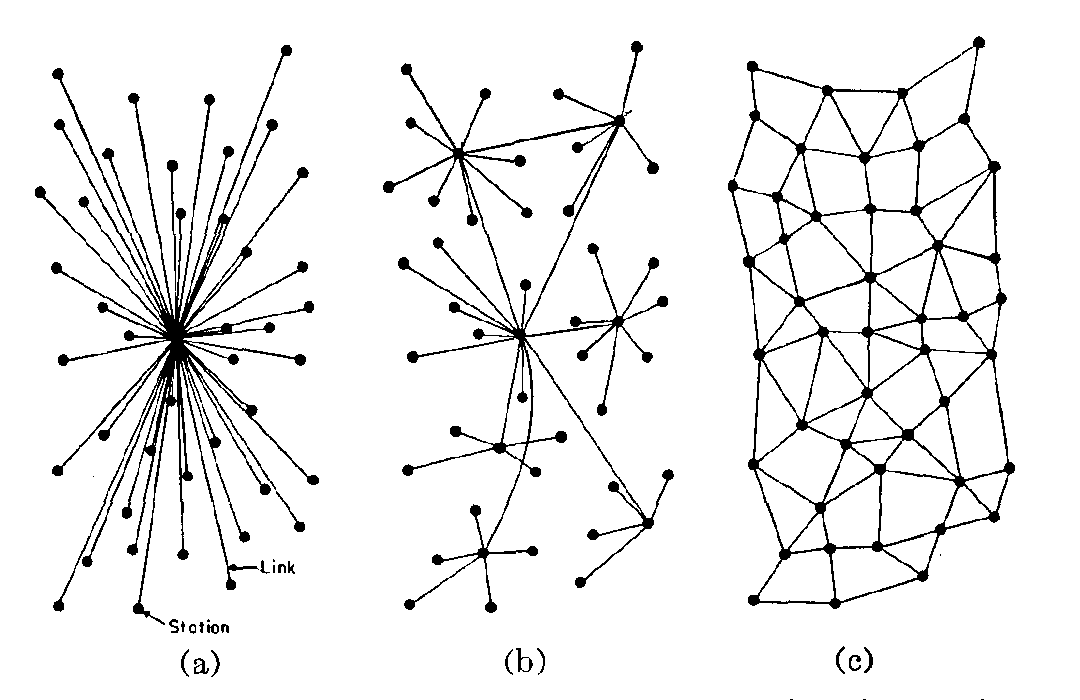
\includegraphics{chapters/img/baran1964-networks.png}

}

\caption{Réseaux~: (a) centralisé~; (b) décentralisé~; (c) distribué.
(Paul Baran, «~\emph{On Distributed Communications Networks}~», 1964)}

\end{figure}%

Le premier réseau d'Internet tire son origine dans la recherche
militaire. Il s'agissait du réseau ARPANET, conçu par l'ARPA, une agence
de recherche technique rattachée au département de la
Défense\footnote{L'ARPA (\emph{Advanced Research Projects Agency},
  «~Agence pour les projets de recherche avancée~») a été créée en 1958.
  Elle a été rebaptisée DARPA (\emph{Defense Advanced Research Projects
  Agency}, «~Agence pour les projets de recherche avancée de défense~»)
  en 1972. Elle est brièvement redevenue l'ARPA en 1993 avant d'adopter
  définitivement le nom de DARPA en 1996.}. Le but était de développer
un réseau de communication qui puisse résister aux attaques nucléaires
dans le cadre de la Guerre froide. Par la suite, d'autres réseaux se
sont développés de manière similaire dans le monde
militaro-universitaire comme le réseau du NPL au Royaume-Uni, le Merit
Network aux États-Unis ou le réseau Cyclades en France.

Le concept proprement dit d'Internet est apparu en 1974, avec
l'émergence d'une suite de protocoles facilitant l'interconnexion des
réseaux~: la suite TCP/IP\footnote{Vinton G. Cerf, Robert E. Kahn,
  «~\emph{A Protocol for Packet Network Intercommunication}~», in
  \emph{IEEE Transactions on Communications}, vol.~22, no. 5, mai 1974,
  pp.~637--648~:
  \url{https://www.cs.princeton.edu/courses/archive/fall06/cos561/papers/cerf74.pdf}.}.
Ces protocoles permettaient de standardiser la communication des
paquets. La standardisation a été finalisée avec la publication de la
version 4 de IP et de la version 4 de TCP en 1981, et avec leur
intégration dans ARPANET (le réseau fédérateur d'Internet) en 1983. En
1985, a été créé le NSFNET, qui a rapidement pris de l'ampleur, à tel
point qu'il a remplacé ARPANET en tant que réseau fédérateur. Le projet
ARPANET a été officiellement mis hors service en 1990. Mais on pouvait
considérer qu'Internet était alors lancé.

Internet a provoqué un choc sans précédent sur la possibilité de
diffusion des informations. Toutefois, son développement et son adoption
ont été progressifs, à mesure que les gens estimaient son potentiel et
son utilité. Cette croissance est passée par l'apparition de cas
d'utilisation diverses qui ont amené de plus en plus de gens à utiliser
le réseau des réseaux.

Le courrier électronique a été la première application d'Internet. Au
début, il s'agissait d'envoyer des textes par l'intermédiaire du
protocole FTP, puis des protocoles spécifiques ont été développés dans
les années 80. Le premier courriel a été envoyé en 1971. Les listes de
diffusion sont également apparues rapidement avec le développement de
logiciels permettant d'envoyer le même message à un ensemble de
personnes. Le logiciel LISTSERV est ainsi sorti en 1986, Majordomo en
1992, GNU Mailman en 1999.

Un autre cas d'utilisation est l'émergence de forums de discussions, qui
permettaient aux gens de discuter publiquement de sujets spécifiques.
Usenet, un réseau de forums de discussion, a ainsi été lancé en 1980 et
est devenu entièrement compatible avec Internet en 1986. L'utilisateur y
accédait par un logiciel appelé un lecteur de nouvelles. Usenet a été
très populaire à la fin des années 80 et au cours des années 90,
notamment grâce aux universités. C'est de Usenet que provient le concept
de «~septembre éternel~», qui fait référence au mois de septembre 1993,
durant lequel de nombreux nouveaux utilisateurs étaient arrivés, faisant
drastiquement baisser la qualité du discours, tant au niveau du fond que
de la forme\footnote{«~Le mois de septembre 1993 entrera dans l'histoire
  du net comme le mois de septembre qui n'a jamais pris fin.~» -- Dave
  Fischer, \emph{Re: longest USENET thread ever}, 26/01/1994 01:58:52
  UTC~:
  \url{https://groups.google.com/g/alt.folklore.computers/c/wF4CpYbWuuA/m/jS6ZOyJd10sJ}.}.
Usenet a été la cause du développement des premiers fournisseurs d'accès
à Internet (FAI), qui permettaient à leurs clients d'y accéder sans
restrictions, sans matériel nécessaire, contre le paiement d'un
abonnement. Notons enfin que Usenet a été cité par Satoshi Nakamoto dans
le livre blanc de Bitcoin et dans plusieurs de ses messages, ce qui
témoigne de son influence dans la cyberculture.

C'est également à cette époque qu'est apparu le protocole de
communication textuelle IRC (pour \emph{Internet Relay Chat}), qui
permettait à des individus d'échanger des messages en temps réel.

Mais l'évènement vraiment déterminant dans le développement d'Internet a
été l'arrivée du Web, qui a réellement encouragé l'afflux du grand
public. Celui-ci a été conçu en 1989 par le chercheur Tim Berners-Lee
pour le compte du CERN, qui a été aidé par l'ingénieur Robert Cailliau
pour en définir les spécificités. Le modèle a été finalement rendu
public en août 1991.

Le World Wide Web, abrégé communément en Web, et parfois appelé «~la
Toile~» en français, est un système hypertexte public fonctionnant sur
Internet, c'est-à-dire un système permettant de passer d'une page à
l'autre (via des hyperliens) sans devoir revenir à la racine. Même si
l'idée n'était pas nouvelle (le concept d'hypertexte avait été inventé
par Ted Nelson en 1965, dans le cadre de son projet Xanadu), le Web
innovait par trois caractéristiques~: les adresses sous forme d'URL, le
protocole de communication HTTP, et le langage informatique HTML.

L'accès à la Toile se faisait par le biais d'un navigateur Web développé
par Berners-Lee, baptisé WorldWideWeb, qui ne constituait guère plus
qu'une preuve de concept. Ainsi, le Web n'a vraiment décollé que grâce
aux navigateurs Mosaic, créé en 1993, et surtout Netscape, conçu en
1994. Le Web a engendré un engouement sans précédent, notamment grâce à
l'idée du commerce électronique. Cela a finalement abouti à une bulle
financière appelée la bulle Internet (que les anglophones nomment la
\emph{dot-com bubble}), qui a éclaté en mars 2000.

Les années 2000 ont aussi été marquées par le développement du partage
de fichiers en pair-à-pair. En 1999, Napster permettait de partager de
la musique avec d'autres utilisateurs. Néanmoins, il reposait sur un
serveur central pour référencer les fichiers, ce qui l'a contraint à
fermer en 2001 sous la pression de la RIAA, l'association représentant
l'industrie du disque aux États-Unis.

Afin de résoudre ce problème, des protocoles purement pair à pair sont
apparus. Il s'agissait de créer un réseau où tous les ordinateurs
(appelés nœuds) possédaient le même niveau de privilège, par opposition
au modèle client-serveur, de sorte qu'il n'y ait plus de point de
défaillance unique à attaquer pour faire cesser le partage. C'était le
cas de Gnutella et de eDonkey, tous deux créés en 2000. Mais surtout
c'était le cas de BitTorrent, dont la première version a été publiée en
2001\footnote{Bram Cohen, \emph{BitTorrent - a new P2P app}, 2 juillet
  2001, archive~:
  \url{https://web.archive.org/web/20080129085545/http://finance.groups.yahoo.com/group/decentralization/message/3160}.}.
Ces protocoles formaient une alternative beaucoup plus fiable puisqu'il
fallait poursuivre chaque utilisateur individuellement, ce qui
représentait une charge considérable pour l'État.

Une dernière innovation a été le routage en ognon qui venait ajouter de
la confidentialité dans la transmission de données. Le routage en ognon
a été inventé en 1996 par Paul Syverson, aux côtés de David Goldschlag
et Michael Reed, pour le compte du \emph{Naval Research Laboratory}, un
laboratoire de recherche rattaché à la Navy\footnote{David M.
  Goldschlag, Michael G. Reed, Paul F. Syverson, «~\emph{Hiding Routing
  Information}~», in \emph{Proceedings of the First International
  Workshop on Information Hiding}, mai 1996, pp.~137---150~:
  \url{https://www.onion-router.net/Publications/IH-1996.pdf}.}. Les
trois hommes avaient pour mission de construire un réseau de mélange
pour protéger les communications des agences étasuniennes. La mise en
œuvre de cette technique a été réalisée quelques années plus tard, par
le biais du réseau Tor, dont le nom est l'acronyme de \emph{The Onion
Router} et qui a été lancé en 2002 grâce à une subvention de la DARPA.
Il a été rendu public en 2003, afin d'agrandir l'ensemble d'anonymat
dans lequel pouvaient se fondre les communications fédérales. Cela avait
l'avantage de créer un réseau anonyme dans lequel pouvaient œuvrer les
hors-la-loi.

Internet, et plus particulièrement le partage de pair à pair et le
routage en ognon, semblaient donner la possibilité aux gens de continuer
leurs activités malgré la réticence des autorités en charge, de sorte
qu'elles ont inspiré la conception originelle de Bitcoin. Par son
architecture distribuée, le réseau permettait de répartir les risques
pour ne pas subir une attaque qui puisse mettre le système à genoux.
Satoshi écrivait ainsi dans son courriel du 6 novembre 2008~:

«~Les États sont bons pour couper les têtes des réseaux contrôlés de
manière centralisée comme Napster, mais les réseaux purement pair à pair
comme Gnutella et Tor semblent tenir le coup\footnote{Satoshi Nakamoto,
  \emph{Re: Bitcoin P2P e-cash paper}, 06/11/2008 20:15:40 UTC~:
  \url{https://www.metzdowd.com/pipermail/cryptography/2008-November/014823.html}.}.~»

\section*{La philosophie du logiciel
libre}\label{la-philosophie-du-logiciel-libre}
\addcontentsline{toc}{section}{La philosophie du logiciel libre}

\markright{La philosophie du logiciel libre}

La possibilité de diffusion des informations apportée par l'émergence
d'Internet a remis au goût du jour la critique à l'encontre de la
«~propriété intellectuelle~», c'est-à-dire du monopole intellectuel
exercé par certaines personnes sur certaines idées. En effet, il
devenait facile d'accéder à l'information et de la propager ce qui
rendait l'application de cette propriété beaucoup plus complexe. De ce
fait, pour un certain nombre de personnes, les restrictions liées à ce
monopole paraissaient totalement absurdes.

Le «~propriété intellectuelle~» est un privilège accordé à un acteur
économique sur une production de l'esprit, qui peut être une invention
industrielle (auquel cas on parle de brevet) ou une création littéraire
ou artistique (auquel cas on parle de droit d'auteur). Il ne s'agit pas
simplement d'autoriser l'auteur d'une invention ou d'une œuvre à
l'utiliser ou à la diffuser~; il s'agit d'interdire à tous les autres de
l'utiliser ou de la diffuser sans son autorisation.

Le monopole intellectuel est par essence contraire au droit naturel en
raison de l'absence de rareté liée à l'information\footnote{N. Stephan
  Kinsella, «~\emph{Against Intellectual Property}~», in \emph{Journal
  of Libertarian Studies}, vol.~15, no. 2, 2001, pp.~1--53~:
  \url{https://cdn.mises.org/Against\%20Intellectual\%20Property_2.pdf}.}.
Pour le dire autrement, copier n'est pas voler. Thomas Jefferson, qui a
pourtant participé à l'établissement du bureau américain des brevets,
écrivait ainsi en 1813~:

«~Celui qui reçoit une idée de moi reçoit un savoir sans diminuer le
mien~; tout comme celui qui allume sa bougie à la mienne reçoit la
lumière sans me plonger dans la pénombre\footnote{Thomas Jefferson,
  \emph{Letter to Isaac McPherson}, 13 août 1813~:
  \url{https://press-pubs.uchicago.edu/founders/documents/a1_8_8s12.html}.}.~»

Le monopole intellectuel permet à des personnes de toucher des
redevances sans avoir signé un quelconque contrat avec celui qui les
paie. Il encourage la consolidation de l'activité économique au sein de
grandes entreprises. Dans le domaine informatique, il a permis à des
sociétés de devenir de grands empires reposant sur le paiement de
licences de leurs logiciels «~propriétaires~». L'exemple le plus parlant
est celui de Bill Gates et de son entreprise Microsoft. Il permet de
contrôler l'utilisation d'une œuvre, et par conséquent d'influencer la
culture d'une société.

La manière légale de s'opposer à cet ensemble de privilèges dans
l'informatique a été l'émergence des licences libres. Celles-ci
permettaient de prendre l'adversaire à son propre jeu en publiant un
contenu sous une licence interdisant à quiconque de se l'approprier ou
de l'inclure dans un contenu non libre. Ces licences ont émergé dans le
cadre du développement logiciel, qui était soumis au droit d'auteur aux
États-Unis.

Le mouvement a été initié dans les années 80 par Richard Stallman, un
physicien ayant grandi à New York et ayant étudié à Harvard. Ce dernier
avait travaillé pour le département de recherche en intelligence
artificielle au MIT où il avait été introduit à la culture des
\emph{hackers} et fait l'expérience des problématiques posées par les
licences dans le cadre du développement du langage LISP.

Il a fondé le projet GNU en 1983 dans le but de concevoir une
alternative entièrement libre au système d'exploitation UNIX. Le projet
a été lancé par un courriel diffusé sur le forum Usenet
net.unix-wizards. En 1985, il écrivait le manifeste GNU\footnote{Richard
  M. Stallman, \emph{The GNU Manifesto}, mars 1985~:
  \url{https://www.gnu.org/gnu/manifesto.en.html}.} et fondait la
\emph{Free Software Foundation}, ce qui marquait la naissance du
mouvement du logiciel libre, et de la mouvance libriste en général.

Richard Stallman a formellement décrit la notion de logiciel libre pour
la première fois en 1986, au sein du premier bulletin d'informations de
GNU, qu'il réduisait à deux libertés de base~:

«~Premièrement, la liberté de copier un programme et de le redistribuer
à vos voisins, qu'ils puissent ainsi l'utiliser aussi bien que vous.
Deuxièmement, la liberté de modifier un programme, que vous puissiez le
contrôler plutôt qu'il vous contrôle~; pour cela, le code doit vous être
accessible\footnote{Richard M. Stallman, \emph{What is the Free Software
  Foundation?}, février 1986~:
  \url{https://www.gnu.org/bulletins/bull1.txt}.}.~»

Il a par la suite raffiné cette définition pour qu'elle inclue quatre
libertés fondamentales~: la liberté d'utiliser le code dans n'importe
quel but, la liberté de l'étudier et de le modifier, la liberté de le
distribuer sans restriction et la liberté d'en distribuer des versions
modifiées.

Deux types de licences libres se sont distingués~: le type permissif, et
le type contaminant dit \emph{copyleft}. Le premier type de licence
exigeait que le code soit librement utilisable, copiable, distribuable
et modifiable tout en permettant la réutilisation dans un programme non
libre. Le second type était encore plus restrictif et imposait à tout
programme utilisant le code d'être publié sous la même licence.

La première licence libre a été la licence MIT, qui a été développée par
le \emph{Massachusetts Institute of Technology} à partir de 1985.
Licence permissive, elle était initialement présente au sein du
protocole de fenêtrage \emph{X Window System} développé conjointement
avec la DEC et IBM. Une version standarde a été publiée en 1987 (X11),
puis sa version finale a été publiée en 1998 pour être utilisée pour la
bibliothèque Expat.

Une autre licence permissive à apparaître rapidement a été la licence
BSD, dont la première version a été publiée en 1988 pour distribuer,
comme son nom l'indique, le code du système d'exploitation BSD.
Plusieurs variantes de cette licence ont été publiées au cours des
années~: la licence BSD proprement dite, à 4 clauses, en 1990~; la
licence BSD modifiée, à 3 clauses, en 1999~; la licence FreeBSD, à 2
clauses, en 1999 également~; et la licence BSD à zéro clause en 2013.

La première licence contaminante (\emph{copyleft}) a été la \emph{GNU
General Public License}, plus connue sous l'abréviation de GPL, qui a
été créée par Richard Stallman en février 1989. Une version 2 a été
partagée en 1991 et une version 3 en 2007.

La notion d'\emph{open source} ou de code source ouvert n'est venue
qu'après, avec l'invention du terme par Christine Peterson en 1998 et
l'implication d'Eric Steven Raymond. Le terme se rapportait à l'origine
seulement au logiciel libre, dans le but de lever l'ambiguïté de
l'appellation «~\emph{free software}~» en anglais (\emph{free} signifie
à la fois libre et gratuit). Mais il a fini par désigner tous les
logiciels dont le code source était disponible publiquement, qu'ils
soient publiés sous licence libre ou non.

Le code du prototype de Bitcoin (v0.1) a été publié en 2009 sous licence
MIT. Pour un tel système ouvert, il était en effet nécessaire que le
code soit ouvert. De plus, dans le but de réduire au maximum le contrôle
sur le protocole, il fallait que le logiciel soit libre, comme nous
l'expliquerons dans les chapitres~\hyperref[ch:changement]{10} et
\hyperref[ch:determination]{11}.

\section*{La tendance extropienne}\label{la-tendance-extropienne}
\addcontentsline{toc}{section}{La tendance extropienne}

\markright{La tendance extropienne}

L'évolution technique prodigieuse qui s'est produite durant le
\textsc{xx} siècle, et qui ne s'est pas cantonnée à l'informatique et à
la cryptographie, a fait évoluer la vision du monde des gens et la façon
dont ils envisageaient l'avenir. Le développement de procédés de plus en
plus avancés faisait entrevoir des possibilités inédites pour l'homme,
comme l'amélioration de ses capacités, la conception de machines
perfectionnées, la production de substances psychotropes, le voyage
spatial et la création de mondes virtuels. C'est ce qui a mené à la
fondation du mouvement des extropiens au sein de la Silicon Valley à la
fin des années 80.

L'extropianisme était une philosophie transhumaniste libérale optimiste,
qui préconisait l'utilisation proactive de la technique en vue
d'accroître les capacités humaines individuelles et civilisationnelles.
Cette tendance se fondait sur l'extropie, un terme créé pour l'occasion
pour désigner le principe d'organisation qui s'oppose à l'entropie et
qui forme la base de la vie matérielle\footnote{En thermodynamique,
  l'entropie est une grandeur physique qui caractérise le degré de
  désorganisation d'un système physique. Le deuxième principe de la
  thermodynamique énonce que l'entropie d'un système isolé croît avec le
  temps, ce qui implique que l'entropie de l'univers croît à mesure de
  son vieillissement, et qu'il finira par mourir. L'extropie se
  rapproche ainsi de la néguentropie, la baisse locale d'entropie à
  certains endroits, sans être définie de façon aussi formelle.}. Le
cœur de l'extropianisme était ainsi la survie et la prospérité dans un
univers matériel souvent hostile, résolument entropique et finalement
mortel.

Les extropiens ont été précédés par des individus qui ont par la suite
été présentés comme des «~\emph{high-tech hayekians}\footnote{Don
  Lavoie, Howard Baetjer, William Tulloh, «~\emph{High-Tech Hayekians:
  Some Possible Research Topics in the Economics of Computation}~», in
  \emph{Market Process}, vol.~8, 1990~:
  \url{http://www.philsalin.com/hth/hth.html}.}~», dont l'économiste et
futuriste Phil Salin, le pionnier des nanotechnologies Eric Drexler et
l'informaticien et programmeur Mark S. Miller. Ceux-ci adhéraient au
principe de l'ordre spontané -- selon lequel le laissez-faire aboutit à
un ordre supérieur à celui décrété par une autorité constructiviste --
qui avait été développé par les économistes de l'école autrichienne et
qui avait été spécialement mis en valeur par le prix Nobel d'économie
Friedrich Hayek. Ayant assisté à l'accélération de la propagation de
l'information apportée par le développement d'Internet, ils anticipaient
l'ordre nouveau qui allait en résulter. Ils ont cherché à construire des
systèmes qui s'inscrivaient dans cette évolution, comme l'\emph{American
Information Exchange} (AMIX), une place de marché automatisée dédiée à
l'information, et le projet Agorics, un modèle d'échange de calcul
informatique.

Le mouvement extropien a, lui, été fondé en janvier 1988 par Max T.
O'Connor (futur Max More) et Tom W. Bell (aussi connu sous le nom de Tom
Morrow), deux étudiants en philosophie de l'Université de Californie du
Sud qui partageaient la même passion pour l'anticipation futuriste de
l'évolution du monde. Au cours de l'automne 88, ils ont lancé un
magazine appelé \emph{Extropy}, dans lequel ils présentaient leur
doctrine de manière détaillée et autour duquel le mouvement s'est
ensuite construit. Une liste de diffusion a été mise en place durant
l'été 1991 par Perry Metzger, par l'intermédiaire de laquelle les
extropiens pouvaient échanger par courriel sur des sujets divers. Les
extropiens présents dans la région de la baie de San Francisco ne
manquaient pas non plus de se rencontrer dans la vraie vie, au moyen de
ce qu'ils appelaient des Extropaganzas. Un institut, appelé
l'\emph{Extropy Institute}, a aussi été fondé en mai 1992 dans le but de
faire la promotion des principes extropiens. La première conférence
organisée par l'institut, nommée «~Extro 1~», a eu lieu en avril 1994 à
Sunnyvale dans la Silicon Valley. Elle faisait notamment intervenir,
outre Max More et Tom Bell, le spécialiste en robotique Hans Moravec et
le cryptographe Ralph Merkle. Cette conférence a été relatée au cours de
l'automne par le magazine Wired, jetant un peu de lumière sur le
mouvement\footnote{Ed Regis, \emph{Meet the Extropians}, 1 octobre
  1994~: \url{https://www.wired.com/1994/10/extropians/}.}.

Rationaliste, cette doctrine reposait sur quatre principes, définis en
1990~: l'expansion illimitée, l'auto-transformation, l'optimisme
dynamique et la technologie intelligente\footnote{Max More, «~\emph{The
  Extropian Principles}~», in \emph{Extropy}, vol.~6, 1 juillet 1990~:
  \url{https://github.com/Extropians/Extropy/blob/master/ext6.pdf}.}.
L'extropianisme représentait ainsi un transhumanisme, une volonté de
transcender la nature humaine, déjà envisagée auparavant par des
personnes comme Julian Huxley, Robert Ettinger et FM-2030.

La philosophie extropienne n'était pas seulement descriptive, mais
prescriptive. Conformément au principe de l'optimisme dynamique (ou
pragmatique), les extropiens souhaitaient intervenir pour accélérer
l'avènement de l'avenir qu'ils anticipaient. Ils promouvaient ainsi la
recherche et l'expérimentation dans les domaines scientifiques qui
avaient pour but d'améliorer la condition matérielle de l'homme.

D'abord, dans leur lutte contre la mort, les extropiens étaient en
particulier enthousiastes à propos de la cryogénisation, c'est-à-dire de
la conservation à très basse température de corps de défunts dans
l'espoir de les ressusciter grâce à un futur progrès technique.
L'\emph{Alcor Life Extension Foundation}, fondée en 1972 par Fred
Chamberlain \textsc{iii} et sa femme, basée en Arizona, était la
principale organisation qui prenait en charge ce type de service.

Les extropiens étaient également ouvertement hostiles à l'autorité. Ils
promouvaient le principe de l'ordre spontané, décentralisé par nature,
par opposition au technocratisme centralisé, qu'ils considéraient comme
ralentissant le progrès technique\footnote{«~Le progrès durable et la
  prise de décision intelligente et rationnelle requièrent des sources
  d'information et des points de vue diversifiés, rendus possibles par
  les ordres spontanés. La gestion centralisée limite l'exploration, la
  diversité, la liberté et les opinions divergentes. Respecter l'ordre
  spontané, c'est soutenir les institutions volontaristes qui maximisent
  l'autonomie, par opposition aux groupements hiérarchiques rigides et
  autoritaires, qui se caractérisent par leur structure bureaucratique,
  la suppression de l'innovation et de la diversité, et l'étouffement
  des incitations individuelles. Notre compréhension des ordres
  spontanés nous rend très méfiants à l'égard des ``autorités'' qui nous
  sont imposées, et sceptiques à l'égard des dirigeants politiques, de
  l'obéissance inconditionnelle et des traditions non remises en
  question.~» -- Max More, «~\emph{The Extropian Principles v. 2.0}~»,
  \emph{Extropy}, vol.~9, 1992~:
  \url{https://github.com/Extropians/Extropy/blob/master/ext9.pdf}.}.
Certains extropiens s'inspiraient notamment de l'ouvrage de David
Friedman \emph{The Machinery of Freedom}, qui décrivait comment pouvait
s'organiser une société sans État et dont la seconde édition a été
publiée en 1989.

Ensuite, c'est tout naturellement que la cryptographie forte constituait
un des centres d'intérêt des extropiens. Nécessaire pour préserver leur
liberté, elle constituait une des briques de base pour parvenir à leurs
fins. C'est pourquoi le mouvement extropien était en réalité étroitement
lié au mouvement cypherpunk, lui aussi inspiré par le développement
technique, de nombreuses personnes s'investissant dans les deux, comme
Tim May, Hal Finney (qui a été cryogénisé par la Fondation Alcor en
2014) ou Nick Szabo.

Les extropiens s'intéressaient enfin à la monnaie. Une monnaie solide
était en effet nécessaire pour imaginer pouvoir conserver de la valeur à
très long terme, par exemple dans le cas d'une cryogénisation. Le sujet
était ainsi abordé dans le magazine Extropy. En 1993, Hal Finney a
présenté le fonctionnement du système d'argent liquide électronique
eCash\footnote{Hal Finney, \emph{Protecting privacy with electronic
  cash}, \emph{Extropy}, vol.~10, 1993~:
  \url{https://github.com/Extropians/Extropy/blob/master/Extropy-10.pdf}.}.
En 1995, le numéro 15 de la revue a été ouvertement dédié à la monnaie
électronique et à la concurrence des monnaies, comme l'attestait sa
couverture illustrée par un billet de banque privée à l'effigie de
Hayek\footnote{\emph{Extropy}, vol.~15, 1995~:
  \url{https://github.com/Extropians/Extropy/blob/master/ext15.pdf}.}.

\begin{figure}[H]

{\centering 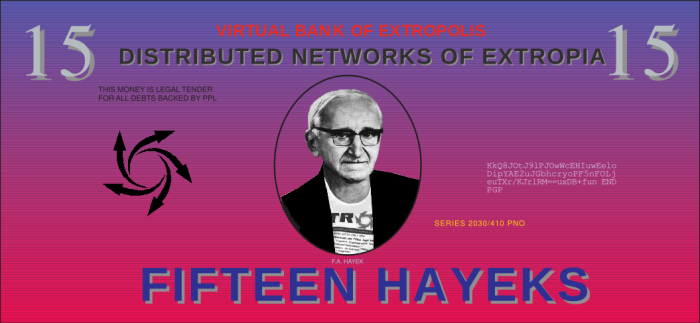
\includegraphics{chapters/img/fifteen-hayeks-note-extropy-15.png}

}

\caption{Le billet fictif de 15 hayeks en couverture du magazine
Extropy.}

\end{figure}%

La monnaie numérique constituait donc l'un des enjeux mis en avant par
les extropiens. Mais ces derniers ne le faisaient pas autant que les
cypherpunks qui, des années plus tard, tenteraient de mettre en pratique
leur connaissance de la cryptographie pour en créer une.

\section*{Le mouvement des
cypherpunks}\label{le-mouvement-des-cypherpunks}
\addcontentsline{toc}{section}{Le mouvement des cypherpunks}

\markright{Le mouvement des cypherpunks}

Le mouvement cypherpunk est apparu en 1992 dans la Silicon Valley. Les
cypherpunks étaient des gens qui prônaient l'utilisation proactive de la
cryptographie en vue d'assurer la confidentialité et la liberté des
individus sur Internet. Ils s'opposaient à la surveillance, à la censure
et à l'exploitation des données personnelles, et préconisaient la
programmation et la publication ouverte de logiciels, préférablement
sous licence libre, dans le but de combattre ces menaces. Leur nom,
calqué sur cyberpunk, était un mot-valise composé des mots anglais
\emph{cypher}, signifiant «~chiffre~» (dans le sens de code secret), et
\emph{punk}, désignant originellement un voyou. Les cypherpunks étaient
donc formellement des rebelles amateurs de cryptographie.

Les cypherpunks s'inspiraient partiellement du cyberpunk, un mouvement
culturel construit autour de la littérature de science-fiction, qui
prenait sa source à la fois dans la sous-culture des punks et dans la
mouvance des hackers. Même si l'esthétique de ce dernier datait de la
fin des années 70, le genre littéraire a largement été inauguré par
l'écrivain William Gibson via la publication de ses premières nouvelles
à partir de 1981 et surtout de son roman \emph{Neuromancien}. Le mot,
qui faisait référence à la cybernétique, c'est-à-dire la science des
systèmes complexes et des réseaux, a quant à lui été inventé en 1983 par
Bruce Bethke, et a été popularisé par Gardner Dozois en décembre 1984
dans un éditorial pour le Washington Post.

La caractéristique principale du genre cyberpunk était de décrire un
futur dystopique où la technique de pointe était omniprésente (implants
informatiques, réalité augmentée, réalité virtuelle, intelligence
artificielle, robots) et où la société était sujette à la consommation à
outrance (drogue, sexe, etc.), au crime généralisé et à l'avarice des
corporations. Le cyberpunk décrivait ainsi un monde combinant haute
technologie et bassesse humaine, pour reprendre l'expression de Bruce
Sterling, dont le héros tentait de s'extraire tant bien que mal.

De ce genre cyberpunk est né tout un mouvement d'individus qui
partageaient la même vision du monde, formant notamment une
contreculture cyberdélique, née de la fusion de la cyberculture et du
psychédélisme. Cette sous-culture en vogue dans la Silicon Valley était
incarnée par la revue \emph{High Frontiers}, fondée en 1984 par R. U.
Sirius, qui est plus tard devenue \emph{Reality Hackers} puis
\emph{Mondo 2000}.

Les cypherpunks tiraient leur inspiration de ce mouvement. Toutefois,
ils n'étaient pas pour autant des cyberpunks~: s'ils avaient bien
conscience des scénarios dystopiques qui pouvaient dériver de
l'évolution technique (notamment en ce qui concerne la surveillance),
ils ne partageaient pas la vision pessimiste relayée par le cyberpunk.
De ce fait, le mouvement cypherpunk constituait en quelque sorte une
réaction au cyberpunk, dans le sens où il postulait, à l'instar des
extropiens, que l'évolution technique pouvait amener les êtres humains à
s'émanciper plutôt qu'à tomber dans l'esclavage mutuel.

Les cypherpunks basaient en particulier leurs réflexions sur une longue
nouvelle publiée en 1980 par l'auteur de science-fiction Vernor Vinge,
intitulée \emph{True Names}. Cette nouvelle, qui abordait des thèmes
propres au genre cyberpunk sans strictement en faire partie, contait
l'histoire de Roger Pollack, un individu agissant au sein d'un groupe de
pirates dans un monde virtuel appelé «~\emph{The Other Plane}~»,
utilisant le pseudonyme de Mr.~Slippery et faisant attention à ne
surtout pas révéler son «~Vrai Nom~» (à savoir son nom civil) au risque
de subir une «~Vraie Mort~» (par exécution étatique). Cet enjeu
correspondait par conséquent à l'enjeu principal de la cryptographie~:
la préservation de l'anonymat dans le but de conserver sa liberté et,
\emph{in fine}, sa vie.

Les cypherpunks avaient ainsi le regard tourné vers l'avenir. Mais leur
préoccupation centrale concernait surtout l'avenir proche~: c'était la
confidentialité dans le cyberespace naissant\footnote{Le terme
  «~cyberespace~» (\emph{cyberspace}) a été forgé par William Gibson
  dans sa nouvelle \emph{Gravé sur Chrome} publiée en juillet 1982, pour
  désigner la représentation virtuelle des flux de données sur Internet.
  Le terme «~matrice~» (\emph{matrix}) était utilisé en tant que
  synonyme.}. C'est pourquoi leur mouvement pouvait rassembler des
optimistes et des pessimistes, des extropiens et des cyberpunks, qui
trouvaient du sens dans cette lutte contre la surveillance de masse.

À l'origine, le mouvement cypherpunk a été le fruit de la pensée et de
l'action de Timothy C. May, dit Tim May. Ce dernier était un
scientifique, ingénieur et informaticien né en 1951 en périphérie de
Washington D.C. Passionné de science-fiction et de physique, il avait
travaillé pour Intel de 1974 à 1986, où il avait contribué à résoudre le
problème des particules alpha dans les circuits intégrés. Il avait
accumulé une certaine fortune au cours de ces années, si bien qu'il
avait décidé de prendre sa retraite (à l'âge de 35 ans) pour se
consacrer à ses passions politiques.

Tim May a rencontré Phil Salin en 1987, avec qui il a pu discuter des
implications de la cryptographie. Ses discussions avec Salin, ainsi
qu'avec d'autres personnes comme Marc Stiegler, l'ont poussé à écrire le
\emph{Manifeste crypto anarchiste} en août 1988. Dans ce manifeste, il
posait les bases de ce qui allait devenir la doctrine des cypherpunks et
décrivait le potentiel d'émancipation individuelle apporté par la
cryptographie et par l'anonymat. Le manifeste, pastiche ironique du
\emph{Manifeste du parti communiste}, décrivait comment l'avènement des
méthodes cryptographiques modernes allait, d'après lui, déstabiliser
l'État en permettant aux individus d'échanger librement de l'information
et de la richesse. En particulier, il écrivait~:

«~Tout comme la technique de l'imprimerie a altéré et réduit le pouvoir
des corporations médiévales et la structure sociale de pouvoir, les
méthodes cryptologiques altèrent fondamentalement la nature de
l'interférence de l'État et des grandes entreprises dans les
transactions économiques\footnote{Timothy C. May, \emph{The Crypto
  Anarchist Manifesto}, 22/11/1992 20:11:24 UTC~:
  \url{https://cypherpunks.venona.com/date/1992/11/msg00204.html}.}.~»

Tim May n'était pas seul à penser de cette manière et communiquait avec
d'autres personnes qui partageaient ses idées. C'était le cas de son ami
Eric Hughes, un jeune mathématicien et programmeur ayant grandi dans une
famille mormone en Virginie près de Washington et à Salt Lake City. Ce
dernier avait travaillé brièvement pour DigiCash à Amsterdam avant de
revenir sur la côte Ouest. En mai 1992, alors qu'il cherchait à
emménager dans la Silicon Valley, lui et Tim May ont longuement discuté
de cryptographie, à tel point qu'ils ont décidé de reproduire ce type
d'échange avec un plus grand nombre de personnes en organisant des
réunions physiques.

La première réunion du mouvement cypherpunk a ainsi eu lieu au cours de
la journée du 19 septembre 1992, dans la maison d'Eric Hughes à Oakland.
L'accès à cette réunion se faisait uniquement sur invitation afin de
préserver la discrétion du groupe. Libertariens pour la plupart,
extropiens pour certains, les invités étaient des connaissances de May
et Hughes issues de la communauté des hackers et des entreprises
informatiques de la région. Durant la réunion, Tim May y a lu le
\emph{Manifeste crypto anarchiste}. En guise d'animation, les personnes
conviées ont également participé à un «~jeu de la crypto anarchie~», qui
consistait à simuler un réseau de mélange par l'échange et l'ouverture
d'enveloppes de papier\footnote{Certains détails de la formation des
  cypherpunks sont issus de l'ouvrage \emph{Crypto: How the Code Rebels
  Beat the Government--Saving Privacy in the Digital Age} (pp.~257--266)
  de Steven Levy publié en 2001.}.

Parmi les invités se trouvait John Gilmore, un informaticien américain
connu pour avoir été l'un des premiers employés de Sun Microsystems. Il
avait aussi cocréé la hiérarchie ouverte alt.* sur Usenet et était un
contributeur majeur du projet GNU. Alors en retraite anticipée depuis
1986, tout comme May, il s'était engagé dans l'activisme dans le but de
protéger les libertés civiles sur Internet. En 1989, il avait cofondé
Cygnus Support, une entreprise spécialisée dans le support professionnel
de composants fondés sur GNU. Il avait également participé à la création
de l'\emph{Electronic Frontier Foundation} (EFF), une ONG internationale
de protection des libertés sur Internet, aux côtés de Mitch Kapor et de
John Perry Barlow en 1990. Lui aussi voyait la cryptographie comme un
moyen de libération individuelle\footnote{«~Et si nous pouvions
  construire une société dans laquelle les informations ne seraient
  jamais collectées~? {[}...{]} C'est le genre de société que je veux
  construire. Je veux que soit garantie - par la physique et la
  mathématique, pas par des lois - la possibilité de bénéficier de
  choses telles qu'une véritable confidentialité des communications
  personnelles, {[}...{]} une véritable confidentialité des
  enregistrements personnels, {[}...{]} une véritable liberté de
  commerce, {[}...{]} une véritable confidentialité financière {[}et{]}
  un véritable contrôle de l'identification.~» -- John Gilmore,
  \emph{Privacy, Technology, and the Open Society}, 28 mars 1991~:
  \url{http://www.toad.com/gnu/cfp.talk.txt}~; archive~:
  \url{https://web.archive.org/web/19991003163945/http://www.toad.com/gnu/cfp.talk.txt}.}.

Une autre personne présente durant cette réunion fondatrice était
l'activiste Judith Milhon, une femme née en 1939 qui avait participé au
mouvement des droits civiques pour l'abolition des discriminations
raciales dans les années 60 et avait été emprisonnée pour désobéissance
civile. Programmeuse, hackeuse, elle était alors la coéditrice de la
revue cyberpunk \emph{Mondo 2000}, à laquelle elle participait sous le
nom de plume de St.~Jude. Elle était également la compagne d'Eric
Hughes, malgré leur grande différence d'âge.

C'est elle qui a donné leur nom aux cypherpunks lors de cette réunion,
sur le ton de la plaisanterie. «~Je pense que vous êtes des
cryptoanarchistes -- ce que j'appellerais des cypherpunks~!~», a-t-elle
écrit par la suite\footnote{Judith Milhon, \emph{secretions}, 25/09/1992
  10:01:26 UTC~:
  \url{https://cypherpunks.venona.com/date/1992/09/msg00013.html}.}. Le
terme capturait bien l'esprit de la cryptoanarchie, tout en donnant au
mouvement un côté moins formel et dogmatique. En effet, les gens
préoccupés par ces enjeux n'étaient pas tous anarchistes~: ils pouvaient
s'opposer fermement à l'autoritarisme et à la surveillance, sans pour
autant vouloir remettre en cause les fondements même de
l'État\footnote{«~De plus, cela donne à tort l'impression que
  ``cypherpunk'' est synonyme d'\,``anarchiste''. Il se trouve que je
  suis anarchiste, mais ce n'est pas ce en quoi croient la plupart des
  personnes associées au terme ``cypherpunk'', et il n'est pas juste de
  les dépeindre ainsi -- bon sang, de nombreuses personnes sur cette
  liste de diffusion sont ouvertement hostiles à l'anarchisme. Je ne
  veux pas que les gens pensent qu'il faut détester l'idée même d'État
  pour aimer la cryptographie.~» -- Perry E. Metzger, \emph{Re: PC Expo
  summary!!}, 01/07/1994 12:13:09 UTC~:
  \url{https://cypherpunks.venona.com/date/1994/07/msg00014.html}.}.
C'est ce côté informel qui a fait que le terme a été adopté
immédiatement.

Après la réunion, Eric Hughes, avec l'aide de Hugh Daniel, a créé une
liste de diffusion de courrier électronique nommée «~Cypherpunks~». Le
courriel de bienvenue a été envoyé dans la soirée du 21 septembre (PDT).
La liste était relayée par le serveur associé au nom de domaine toad.com
appartenant à John Gilmore. Ce dernier a aussi offert la disponibilité
des locaux de Cygnus pour les réunions ultérieures.

La liste a accueilli de nombreuses discussions relatives à la
cryptographie et à son utilisation concrète, dont notamment l'argent
liquide électronique. Beaucoup de gens sont intervenus dès les premiers
mois, comme par exemple l'ancien pirate téléphonique John Draper. En un
an à peine, la liste recensait ainsi plus de 500 participants.

L'un de ces participants était Harold T. Finney \textsc{ii}, dit Hal
Finney, informaticien et cryptographe américain, diplômé de Caltech et
programmeur de jeux vidéos pour les consoles Intellivision et Atari VCS.
Extropien et enthousiasmé par la popularisation d'Internet, il était
obsédé par la cryptographie, à tel point qu'il était rentré en contact
avec Phil Zimmermann pour travailler avec lui sur la version 2.0 de PGP,
sortie le 2 septembre 1992. Hal Finney était aussi fasciné par les idées
de David Chaum. En novembre 1992, il écrivait à la liste de diffusion~:

«~Nous voici confrontés aux problèmes de la perte de confidentialité, de
l'informatique envahissante, des bases de données massives, de
l'augmentation de la centralisation -- et Chaum propose une direction à
suivre complètement différente, une direction qui met le pouvoir entre
les mains des individus plutôt qu'entre celles des États et des grandes
entreprises. L'ordinateur peut être utilisé comme un outil pour libérer
et protéger les personnes, plutôt que pour les contrôler\footnote{Hal
  Finney, \emph{Why remailers...}, 16/11/1992 01:30:02 UTC~:
  \url{https://cypherpunks.venona.com/date/1992/11/msg00108.html}.}.~»

La vision des cypherpunks était claire~: mettre en pratique ce qui avait
été jusque-là de vagues spéculations. Il était en effet stérile de
théoriser des choses si cela ne se traduisait pas par des actions
concrètes. Cet esprit pratique a été parfaitement résumé par Eric Hughes
dans son \emph{Manifeste d'un Cypherpunk} envoyé à la liste de diffusion
en mars 1993, où il écrivait alors~:

«~Nous devons défendre notre propre vie privée si nous voulons en avoir
une. Nous devons nous rassembler et créer des systèmes qui rendent
possibles les transactions anonymes. Depuis des siècles, les gens
défendent leur vie privée par des chuchotements, par l'obscurité, par
des enveloppes, des portes fermées, des poignées de main secrètes et des
messagers. Les techniques du passé ne permettaient pas une forte
confidentialité~; les techniques électroniques, elles, le permettent.

Nous, les Cypherpunks, nous consacrons à construire des systèmes
anonymes. Nous défendons notre vie privée avec la cryptographie, avec
les systèmes anonymes de transfert de courriels, avec les signatures
numériques, et avec la monnaie électronique.

Les Cypherpunks écrivent du code. Nous savons que quelqu'un doit
concevoir des logiciels pour défendre la vie privée en général, et
puisque nous ne pouvons pas avoir de vie privée si tout le monde n'en a
pas, nous allons nous en charger. Nous publions notre code pour que nos
collègues Cypherpunks puissent le mettre en pratique et expérimenter
avec. Notre code est libre d'utilisation pour tous, dans le monde
entier. Nous ne nous soucions guère que vous n'approuviez pas les
logiciels que nous concevons. Nous savons que les logiciels ne peuvent
pas être détruits et qu'un système largement dispersé ne peut pas être
arrêté\footnote{Eric Hughes, \emph{RANTS: A Cypherpunk's Manifesto},
  17/03/1993 19:51:06 UTC~:
  \url{https://cypherpunks.venona.com/date/1993/03/msg00392.html}.}.~»

Deux mois plus tard, en mai 93, le mouvement était définitivement
lancé~: les cypherpunks faisaient la une du magazine Wired, récemment
fondé dans le but de parler de l'incidence culturelle, économique et
politique des techniques émergentes. Tim May, Eric Hughes et John
Gilmore apparaissaient masqués sur la couverture, et un long article
détaillait leurs idées et leurs revendications\footnote{Steven Levy,
  «~\emph{Crypto Rebels}~», \emph{Wired}, 1 février 1993~:
  \url{https://www.wired.com/1993/02/crypto-rebels/}. -- Par la suite,
  le mouvement a également été présenté dans les revues \emph{Whole
  Earth Review} et \emph{The Village Voice}.}. C'était la préfiguration
du rôle qu'ont joué par la suite les cypherpunks dans la sauvegarde de
la liberté sur Internet.

\section*{L'action des cypherpunks pour la
liberté}\label{laction-des-cypherpunks-pour-la-libertuxe9}
\addcontentsline{toc}{section}{L'action des cypherpunks pour la liberté}

\markright{L'action des cypherpunks pour la liberté}

Le mouvement cypherpunk est né juste après le triomphe des États-Unis
dans la guerre froide les opposant à l'URSS et au début de l'adoption
d'Internet par le grand public, amorcée notamment par la popularisation
de Usenet et par l'apparition du World Wide Web. Il est apparu en
quelque sorte «~au bon moment~» pour accompagner cette mutation majeure
qui a marqué le monde entier.

Le premier accomplissement des cypherpunks a été leur intervention dans
la guerre contre la cryptographie orchestrée par l'État fédéral
étasunien. Cette guerre a été inaugurée en février 1993 par la bataille
contre PGP, lorsque Phil Zimmermann a été poursuivi en justice pour en
avoir publié les deux premières versions en ligne, l'exportation de
produits cryptographiques sans licence étant prohibée par la
réglementation américaine (ITAR).

Cette décision a naturellement suscité une forte réaction de la part des
cypherpunks qui, en réponse à la tentative d'application de cette
réglementation absurde, se sont mis à partager le code de chiffrement
dans une démarche de désobéissance civile. Le jeune britannique Adam
Back l'a ainsi fait imprimer sur des t-shirts qu'il distribuait aux
autres et certains ont été jusqu'à se le tatouer sur leur corps. En
1995, Phil Zimmermann a publié la version 2.6.2 de PGP dans un livre,
dans le but de réduire au maximum la distinction entre le code et
l'expression, cette dernière étant protégée par le premier amendement de
la Constitution des États-Unis.

Les charges contre Zimmermann ont finalement été abandonnées en 1996,
notamment grâce au soutien de membres du MIT. Cela lui a permis de créer
son entreprise pour travailler sur PGP et engager des employés, comme
Hal Finney. En novembre de la même année, Bill Clinton signait l'Ordre
exécutif 13026 qui assouplissait considérablement les restrictions sur
l'exportation des produits cryptographiques.

Cependant, la guerre contre la cryptographie ne s'arrêtait pas là. En
effet, elle ne concernait pas que l'interdiction d'utiliser la
cryptographie forte, mais également l'obligation pour les constructeurs
de matériel informatique d'intégrer des portes dérobées dans leurs
produits. Le projet de loi sénatoriale 266, proposé par Joe Biden en
1991, devait ainsi faire en sorte que tous les appareils de
communication puissent être surveillés par l'État fédéral~:

«~Le Congrès estime que les fournisseurs de services de communications
électroniques et les fabricants d'équipements de services de
communications électroniques doivent veiller à ce que les systèmes de
communications permettent au gouvernement d'obtenir le contenu en texte
clair des communications vocales, informatiques et autres lorsque la loi
l'autorise de manière appropriée\footnote{\emph{Comprehensive
  Counter-Terrorism Act of 1991}, 24 janvier 1991~:
  \url{https://www.congress.gov/bill/102nd-congress/senate-bill/266/text}.}.~»

Ce projet s'est matérialisé le 16 avril 1993 par l'annonce de la puce
Clipper par la Maison-Blanche, un cryptoprocesseur servant à chiffrer
les messages vocaux et les données, qui implémentait (au moyen de son
algorithme Skipjack) un dispositif d'autorité de séquestre permettant
aux agences étasuniennes de déchiffrer les communications au besoin.
Cette puce était développée et produite par la NSA et était destinée à
équiper les appareils électroniques vendus au grand public. La
Maison-Blanche se justifiait en prétendant que la puce pourrait «~à la
fois fournir aux citoyens respectueux de la loi un accès au chiffrement
dont ils ont besoin et empêcher les criminels de l'utiliser pour cacher
leurs activités illégales\footnote{The White House, \emph{White House
  Annoucement of the Clipper Initiative}, 16 avril 1993~:
  \url{https://groups.csail.mit.edu/mac/classes/6.805/articles/crypto/clipper-announcement.html}.}~».

Cette annonce a provoqué une levée de boucliers chez les cypherpunks qui
y voyaient un projet orwellien et s'y sont opposés en bloc. Cependant,
la lutte n'a pas été longue~: en juin 1994, le cypherpunk Matt Blaze a
découvert une vulnérabilité au sein du dispositif d'autorité de
séquestre, qui rendait le dispositif inefficace et permettait à la puce
d'être utilisée pour chiffrer les données normalement. À partir de là,
le projet a perdu progressivement en ampleur pour être définitivement
abandonné en 1996. La liberté avait gagné, au moins
temporairement\footnote{Cette victoire contre la puce Clipper n'a pas
  empêché les agences étasuniennes d'espionner leur propre population de
  manière massive, comme l'ont montré les révélations d'Edward Snowden
  en 2013. -- Voir Glenn Greenwald, \emph{NSA collecting phone records
  of millions of Verizon customers daily}, 6 juin 2013~:
  \url{https://www.theguardian.com/world/2013/jun/06/nsa-phone-records-verizon-court-order}.}.

Comme on l'a observé, l'optique des cypherpunks était d'être dans
l'action, d'écrire du code et de partager des programmes qui puissent
être utilisés. Ils se sont donc focalisés sur la construction de
systèmes axés sur trois aspects majeurs~: la protection de la vie
privée, la diffusion de l'information et le commerce en ligne.

Le premier domaine d'innovation a été celui des serveurs de courriel
anonyme, qui permettaient de retransmettre les courriers électroniques
de façon à masquer l'identité de leur expéditeur. Le premier serveur de
ce type a été mis en place par Eric Hughes et Hal Finney pour la liste
des cypherpunks dès octobre 1992, et il utilisait PGP pour le
chiffrement. En 1994, Lance Cottrell a amélioré la chose en proposant le
modèle Mixmaster, qui permettait d'envoyer des courriels par paquets de
taille fixe et de les réordonner, pour empêcher le traçage des courriels
par la surveillance de l'activité du serveur.

Outre le courriel, l'objectif des cypherpunks était de rendre la
navigation sur Internet plus anonyme, le fonctionnement du Web étant
trop transparent. C'était l'idée des frères Austin et Hamnett Hill qui
ont lancé le réseau Freedom en 1999 par l'intermédiaire de leur
entreprise Zero-Knowledge Systems, qui employait notamment les
cypherpunks Ian Goldberg et Adam Back. Mais cette expérience s'est
arrêtée en 2001, faute d'utilisation suffisante.

Un projet du même type dans lequel les cypherpunks se sont impliqués
était le réseau Tor, lancé publiquement en 2003, qui se basait, comme on
l'a déjà expliqué, sur le routage en ognon. En effet, si Tor était le
résultat d'une recherche militaire provenant de la Navy, les individus
ayant travaillé sur son implémentation n'en avaient pas moins des
convictions allant dans le sens des cypherpunks. Roger Dingledine et
Nick Mathewson, les deux informaticiens qui ont aidé Paul Syverson dans
cette conception, en faisaient partie~: le premier était derrière le
projet Free Haven, qui avait pour but de développer un système
décentralisé de stockage de données~; le second est crédité pour avoir
créé le programme de serveur de courriel anonyme Mixminion. On peut
également citer le jeune Jacob Appelbaum, qui s'est fortement impliqué
dans le projet Tor entre 2004 et 2016.

Un troisième secteur auquel les cypherpunks ont contribué a été la
fluidification des flux informationnels, notamment face à la censure. En
1993, Tim May a repris le modèle de l'AMIX de Phil Salin pour introduire
un concept de place de marché de l'information appelé BlackNet. Cette
plateforme devait servir à échanger des secrets commerciaux, des
recettes de fabrication, des techniques relatives aux nanotechnologies,
des informations sur les décisions d'entreprises, au moyen de
«~CryptoCredits~», la monnaie interne du système. Il s'agissait donc de
libérer l'information des contraintes étatiques~: «~BlackNet n'est
officiellement affilié à aucune idéologie, mais considère les
États-nations, les lois d'exportation, les lois sur les brevets, les
considérations de sécurité nationale, etc. comme des reliques de l'ère
pré-cyberspatiale~», écrivait Tim May\footnote{Timothy C. May, \emph{no
  subject (file transmission)}, 17 août 1993,
  \url{https://cypherpunks.venona.com/date/1993/08/msg00538.html}.}.

Le concept de BlackNet était une simple expérience de pensée et n'a
jamais été mis en œuvre. Toutefois, il a préfiguré d'autres modèles qui
ont ouvert la voie au partage d'informations sensibles sur Internet.
C'était par exemple le cas de Cryptome, un site web lancé en 1996 par le
cypherpunk John Young pour héberger des documents sensibles et censurés
par les États.

Mais c'était surtout le cas de WikiLeaks, une plateforme facilitant la
publication de documents classifiés fondée en 2006 par l'informaticien
australien Julian Assange. Julian Assange était un cypherpunk assumé~:
il envoyait des courriels sur la liste depuis au moins 1995 et a par la
suite coécrit un livre à ce sujet intitulé \emph{Cypherpunks: Freedom
and the Future of the Internet}. WikiLeaks a permis le développement de
l'activité des lanceurs d'alertes (\emph{whistleblowers}) révélant les
agissements illégaux ou injustes de leurs employeurs, et en particulier
des États, largement inaugurée par la publication des Pentagon Papers en
1971 par Daniel Ellsberg. Grâce à l'utilisation du chiffrement et de
Tor, WikiLeaks permettait aux personnes à l'origine des fuites de
conserver leur anonymat.

Enfin, les cypherpunks se sont aussi investis dans le développement du
pair-à-pair. En 2000, le développeur Jim McCoy, cypherpunk de la
première heure, a ainsi lancé Mojo Nation, un projet de plateforme
d'échange de fichiers en pair-à-pair intégrant une devise
interne\footnote{Damien Cave, \emph{The Mojo solution}, 9 octobre 2000~:
  \url{https://www.salon.com/2000/10/09/mojo_nation/}.}. En 2001, un
contributeur au projet, appelé Bram Cohen, s'en est séparé et a lancé
son propre protocole, BitTorrent, qui est rapidement devenu une
référence pour le partage de fichiers. Mojo Nation, alors rebaptisé
Mnet, a été repris par Zooko Wilcox. Ce dernier a lancé son propre
système, Tahoe-LAFS, en 2006.

Mais ce qu'il manquait à tous ces systèmes, c'était une monnaie
numérique robuste qui soit adaptée au cyberespace, chose à laquelle les
cypherpunks aspiraient depuis le début. Leurs modèles possédaient
parfois des unités de compte internes, mais elles étaient très
instables. Malheureusement, une telle monnaie ne serait conçue que des
années plus tard, en 2008, sous la forme de Bitcoin.

Satoshi Nakamoto était-il un cypherpunk~? À notre connaissance, il n'a
pas participé au mouvement originel des années 90, ni ne s'est jamais
réclamé explicitement de celui-ci. Toutefois, il a très clairement été
influencé par l'héritage des cypherpunks comme le suggèrent plusieurs
éléments. D'abord, il semblait bien connaître ce qui s'était passé et de
ce qui avait été fait précédemment dans le domaine de la monnaie
numérique, malgré quelques lacunes (voir le
chapitre~\hyperref[ch:cybermonnaie]{6}). Puis, il a publié le livre
blanc sur la liste de diffusion dédiée à la cryptographie gérée par
Perry Metzger, qui était la digne héritière de la liste des cypherpunks,
dont l'usage avait malheureusement périclité vers 1997. Ensuite, il a
utilisé un pseudonyme et, par de bonnes pratiques comme l'utilisation de
PGP, Tor et Namecheap, il est parvenu à préserver son anonymat malgré
une activité en ligne s'étalant sur presque trois années. Enfin, il a
«~écrit du code~» en programmant un outil émancipateur, conformément à
l'appel à la pratique d'Eric Hughes. Il est donc tout à fait raisonnable
d'associer Satoshi aux cypherpunks, tout en l'en dissociant
partiellement, ne serait-ce parce qu'il est toujours resté très mesuré
dans ses quelques jugements politiques.

\section*{Une guerre perpétuelle}\label{une-guerre-perpuxe9tuelle}
\addcontentsline{toc}{section}{Une guerre perpétuelle}

\markright{Une guerre perpétuelle}

Bitcoin s'inscrit pleinement dans la guerre technologique opposant
l'autorité à la liberté. Son code n'est pas neutre~: il n'est pas une
vague technique qu'on puisse utiliser dans un sens ou dans l'autre, mais
il a pour objectif clair d'amener plus d'autonomie individuelle. Bitcoin
n'est pas un assemblage aléatoire de procédés, mais un objet ancré dans
son époque, qui prend racine dans les mouvements techno-idéologiques qui
l'ont précédé.

Bitcoin est ainsi issu de mouvements qui appellent à la pratique. Les
libristes promouvaient la publication sous licence libre dans le but de
mettre en commun l'ensemble des connaissances de l'humanité. Les
extropiens préconisaient la recherche et l'expérimentation pour
améliorer drastiquement les conditions de vie matérielles de l'être
humain. Les cypherpunks prônaient le fait d'écrire du code afin de
préserver la confidentialité des individus dans le cyberespace. Il est
donc naturel que la communauté de Bitcoin s'inscrive dans la même
démarche en encourageant la pratique monétaire en vue de résister au
contrôle de plus en plus grand de l'État et des banques sur le transfert
d'argent.

Cependant, pour arriver à ce résultat, il a fallu concevoir un système
qui permette de répartir les risques entre les participants sans
nécessiter l'intervention d'un tiers de confiance. Une quête que nous
raconterons dans le prochain chapitre.

\bookmarksetup{startatroot}

\chapter{Cryptocurrency Before Nakamoto}\label{ch:cryptocurrency}

\phantomsection\label{enotezch:6}{}

{L}\textsc{a} cryptocurrency is a form of money that relies entirely on
a computer network connected to the Internet. It is defined within this
network and is transferred through it. It is a currency native to
cyberspace---the new realm created by the rise of the
Internet---conceived as a separate jurisdiction from the physical world.

A more specific type of cryptocurrency is digital cash, which replicates
the properties of physical cash in cyberspace. However, although this
concept dates back to the very emergence of the Internet, it could not
immediately come to fruition due to technical and conceptual
limitations. Digital cash has been the subject of a genuine quest,
involving many individuals eager to use the Internet to create a new
economic paradigm, including the cypherpunks.

Bitcoin is the outcome of this quest. It didn't emerge out of nowhere;
it is the result of reflections, research, and various experiments.
Satoshi Nakamoto's discovery thus represents a breakthrough in a
pre-existing field.

\section*{Monetary Exchange on the
Internet}\label{monetary-exchange-on-the-internet}
\addcontentsline{toc}{section}{Monetary Exchange on the Internet}

\markright{Monetary Exchange on the Internet}

The Internet has generalized the sharing of information and, in doing
so, has created a new space for human interactions: cyberspace. The
emergence of this space naturally led to a demand for monetary exchange,
which manifested through the development of e-commerce in the 1990s. As
Robert Hettinga aptly summarized in 1998:

``Since the invention of the telegraph, settling financial transactions
has faced a problem: how to conduct business at a distance when the
simplest way to execute, clear, and settle a transaction is through the
exchange of bearer certificates\footnote{Robert A. Hettinga,
  \emph{Digital Bearer Settlement}, April 1998:
  \url{http://www.systemics.com/legal/digigold/discovery/postings/Geoecon.pdf}.}.''

The initial solution was to use bank credit. The use of bank credit as a
medium of exchange had gradually become widespread in the West with the
banking of society. Over time, a technical solution prevailed: the
payment card, also called a debit or credit card depending on its
operation. This solution wasn't particularly innovative\footnote{The
  term ``credit card'' was used in 1888 by Edward Bellamy, an American
  socialist writer and journalist and a forerunner of the technocracy
  movement, in his speculative fiction novel \emph{Looking Backward}, to
  describe the payment card used by citizens in his envisioned utopia.
  This type of card later developed in the 1920s--1930s in the U.S.
  through cards issued independently by Western Union, department
  stores, oil companies, and airlines.}, but it became considerably
popular from the 1960s onward, through bank adoption and the formation
of companies specializing in electronic funds transfer like NBI/Visa and
Interbank/MasterCard\footnote{For the origins of the Visa network, see
  David L. Stearns, \emph{Electronic Value Exchange: Origins of the VISA
  Electronic Payment System}, Springer, 2011. The book's title
  references Dee Hock's ambitious project (Visa's founder) to create an
  Electronic Value Exchange (EVE) protocol allowing all transactions to
  be conducted electronically, leading to ``the genesis of a new form of
  global currency.''}.

However, payment by bank card wasn't necessarily suited to cyberspace,
as it was difficult to implement, costly, and not very secure at the
time. This is why various technical solutions for making payments on the
Internet emerged in the mid-1990s, such as CyberCash, First Virtual, or
Open Market. Micropayment systems also appeared, like CyberCoin (managed
by CyberCash), NetBill, and MilliCent.

These systems eventually failed, but it was in this niche that the
PayPal service developed from 1999. It was designed to be easily
accessible (PayPal literally means ``pay friend''): it allowed easy,
fee-free payments between email addresses. Its business model was based
on collecting interest from holding clients' funds in banks, to cover
operating costs and remunerate shareholders. It was, therefore, a
third-layer service built on top of the banking system, itself based on
the central monetary system\footnote{For the history of PayPal's early
  days, see Eric M. Jackson, \emph{The PayPal Wars: Battles With eBay,
  the Media, the Mafia, and the Rest of Planet Earth}, World Ahead Pub.,
  2012.}.

Despite the good intentions of their creators, these systems were
entirely at the mercy of regulators. Those that survived consequently
engaged in surveillance and censorship at an unprecedented level.

The second solution for exchanging value on the Internet was to issue a
new digital currency in a centralized manner, possibly backed by an
existing currency. This approach involved acting without seeking
permission, exploiting the legal gray areas that could exist in a
relatively new field.

Massively multiplayer online games, including the famous MMORPGs,
contributed to instilling the idea of an independent digital currency in
people's minds. Examples include the Token, the native currency of
\emph{Habitat}, one of the first graphical MMORPGs developed in 1985 by
Lucasfilm Games for the Commodore 64. Other examples are the precious
metal coins in \emph{EverQuest} in 1999, the Linden dollar of
\emph{Second Life} in 2003, or the gold in \emph{World of Warcraft} in
2004. All these cases demonstrated that a real economy could emerge from
a virtual currency.

An anecdotal example of this type of digital currency system was the
Hawthorne Exchange, launched on March 24, 1993, on the extropian mailing
list by an individual named Brian Holt Hawthorne. It was a reputation
market for list members, where the unit of account used for exchange was
the Thorne. The system wasn't very accessible or robust, but extropians
used it and gave value to the Thorne in anticipation of the future. Some
exchanges for dollars and services took place between list members.
However, the Hawthorne Exchange was merely an experiment; the Thorne
wasn't intended to be a real currency, and its creator decided to stop
it in '94.

A much more serious system appeared in 1996: e-gold. As described in
Chapter~\hyperref[ch:adversary]{4}, it was a digital gold currency model
whose unit of account was theoretically backed by gold. The system
relied on the company \emph{Gold \& Silver Reserve Inc.} founded by
Douglas Jackson, which stored the physical gold in its vaults. It
enjoyed great success in the 2000s before being shut down in 2007 by the
Secret Service.

However, the problem with this type of currency was that it still
depended on an entity that constituted a single point of failure. Thus,
even if those managing it were well-intentioned, such a system wasn't
robust and couldn't endure in the long term.

The third solution for cryptocurrency was the conception of electronic
cash that was confidential, uncontrolled, and decentralized. The idea
was to minimize the role of the trusted third party as much as possible
so that the currency would closely resemble physical cash in terms of
minimizing required trust. Ideally, the goal was to obtain a ``digital
gold'' that was ``unforgeable, inflation-free, and
untraceable\footnote{Hadon Nash, \emph{Digital gold}, August 24, 1993,
  20:23:30 UTC:
  \url{https://cypherpunks.venona.com/date/1993/08/msg00698.html}.}.''

The cypherpunks considered this type of digital currency essential in
their fight for freedom and privacy. They planned to use such a unit of
account in their projects, as evidenced by the Cryptocredits of
\emph{BlackNet} or the mojo of \emph{Mojo Nation}. Naturally, they
sought to develop such a currency.

However, designing electronic cash---a true cryptocurrency---was no easy
task. The quest to achieve it took many years to bear fruit. And the
first step in this quest was the emergence of eCash, which had the merit
of presenting a coherent proposal that met the cypherpunks'
requirements.

\section*{eCash: Chaumian Electronic
Cash}\label{ecash-chaumian-electronic-cash}
\addcontentsline{toc}{section}{eCash: Chaumian Electronic Cash}

\markright{eCash: Chaumian Electronic Cash}

eCash is a concept of confidential digital currency designed by
cryptographer David Chaum in the 1980s and implemented during the 1990s.
Initially described by Chaum in 1982, it was highlighted in 1985 in his
article titled ``\emph{Security without Identification},'' which
promised to ``render Big Brother obsolete\footnote{David L. Chaum,
  ``\emph{Security without identification: transaction systems to make
  big brother obsolete}'', in \emph{Communications of the ACM}, vol.~28,
  no. 10, October 1985, pp.~1030--1044:
  \url{https://www.cs.ru.nl/~jhh/pub/secsem/chaum1985bigbrother.pdf}.}.''
The model is based on the mechanism of blind signatures, which
guarantees ownership of the currency and transaction anonymity.

The eCash model manages digital banknotes of various denominations that
users can hold. The banknotes are issued and replaced by servers called
banks or mints. When a banknote is transferred, the recipient sends it
to their bank, which verifies it and gives them another in return. The
banks in the system each maintain a ledger of spent banknotes to prevent
double-spending. The system is overseen by a central authority that
issues the necessary permissions.

Issuing a digital banknote uses the blind signature mechanism, as
mentioned. For the user, it essentially involves choosing a large number
and having it signed by their bank, so that this number remains known
only to them. The functioning of this mathematical process is analogous
to signing a physical banknote using carbon paper that represents a
specific amount of monetary units (denomination). Here's how Alice
creates a banknote:

\begin{enumerate}
\def\labelenumi{\arabic{enumi}.}
\tightlist
\item
  Alice creates a banknote using carbon paper (by randomly generating a
  very large number ( x ));
\item
  Alice places the banknote in a sealed envelope (using a commutative
  function ( c ) known only to her);
\item
  Alice sends the envelope containing her banknote to the bank and
  specifies the desired denomination;
\item
  The bank signs the envelope, indicating the amount the banknote
  represents (the bank has a private key for each denomination),
  effectively signing the carbon paper banknote inside;
\item
  The bank returns the envelope to Alice;
\item
  Alice opens the envelope to retrieve her signed banknote (using the
  inverse function ( c' ));
\item
  Alice verifies that the bank's signature is authentic (by checking it
  against the bank's public key associated with the requested
  denomination).
\end{enumerate}

Transferring the signed banknote is done by giving it to someone else.
Thus, when Alice pays Bob for a service, the steps are as follows:
first, Alice transmits the banknote to Bob; then, Bob verifies that it
has been signed by Alice's bank; next, he promptly sends the received
banknote to his bank; finally, Bob's bank checks that the banknote
hasn't already been used and, if valid, signs a new banknote of the same
denomination to give to Bob.

\begin{figure}[H]

{\centering 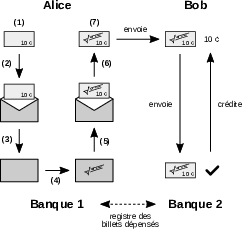
\includegraphics{chapters/img/chaumian-ecash.png}

}

\caption{Creation and replacement of a Chaumian banknote.}

\end{figure}%

Digital banknotes can be issued on their own, forming a base currency.
But they can also be backed by another currency like the dollar. In this
case, the user can return their banknotes to their bank at any time to
retrieve the corresponding amount.

The main consequence of this procedure is that none of the banks in the
system can link the payment to Alice's identity. Alice's bank knows that
a banknote it signed has been spent, but it cannot know for certain that
it belonged to Alice. Bob's bank knows that Bob received the payment and
that it comes from Alice's bank, but nothing more. This is why eCash can
be considered a privacy-respecting model.

However, the system's confidentiality relies on a strong assumption: the
benevolence of the system's banks. Indeed, if a bank wanted to obtain
information related to a particular banknote (e.g., under state
pressure), it could request it from its owner in exchange for
authorizing the transfer. One can imagine an eCash system that fully
complies with surveillance standards, as suggested by Chaum's
implementation for a CBDC conceptualized in 2021\footnote{David L.
  Chaum, Christian Grothoff, Thomas Moser, \emph{How to Issue a Central
  Bank Digital Currency}, March 2021:
  \url{https://www.snb.ch/n/mmr/reference/working_paper_2021_03/source/working_paper_2021_03.n.pdf}.}.

\section*{Magic Money, CyberBucks, and the
Banks}\label{magic-money-cyberbucks-and-the-banks}
\addcontentsline{toc}{section}{Magic Money, CyberBucks, and the Banks}

\markright{Magic Money, CyberBucks, and the Banks}

The concept of eCash was implemented during the 1990s. At the time, the
Web had just emerged, e-commerce was non-existent, and this idea
represented a tremendous opportunity. This implementation was first
undertaken by the cypherpunks through the Magic Money protocol, then by
David Chaum's company, DigiCash, using test tokens called CyberBucks and
deploying within the traditional banking system.

The Magic Money protocol was introduced on the cypherpunks mailing list
on February 4, 1994, by an anonymous developer known as Pr0duct Cypher,
who used PGP for identification. Magic Money allowed users to create
their own currency by running an email server that acted as an eCash
mint\footnote{``Magic Money is a digital cash system designed to be used
  via email. The system is online and untraceable. `Online' means each
  transaction involves an exchange with a server to prevent
  double-spending. `Untraceable' means it's impossible for anyone to
  trace transactions, match a withdrawal with a deposit, or match two
  coins in any way.'' --- Pr0duct Cypher, \emph{Magic Money Digicash
  System}, February 4, 1994, 20:44:27 UTC:
  \url{https://cypherpunks.venona.com/date/1994/02/msg00247.html}.}.
Magic Money used the RSA algorithm and blind signatures, two techniques
patented at the time, making its deployment de facto illegal and
confined to experimentation. Nonetheless, the announcement was
well-received on the list, notably by Hal Finney.

The first system based on Magic Money was launched by Mike Duvos a few
weeks later with the Tacky Tokens, whose coins were issued in
denominations of 1, 2, 5, 10, 20, 50, and 100 units. Despite proposals,
no real transactions occurred, prompting Tim May to wonder ``why digital
cash {[}was{]} not being used\footnote{Timothy C. May, \emph{Why Digital
  Cash is Not Being Used}, May 3, 1994, 19:48:18 UTC:
  \url{https://cypherpunks.venona.com/date/1994/05/msg00155.html}.}.''
Other fanciful implementations of Magic Money followed, such as
GhostMarks, DigiFrancs, or NexusBucks, but none achieved greater
success. Activity quickly dwindled over the weeks.

The concept of eCash was then put into practice by DigiCash B.V., a
company founded by David Chaum in 1990 and based in Amsterdam, whose
mission was to implement the cryptographer's ideas. Several cypherpunks
worked for the company, including Eric Hughes, Bryce Wilcox (the future
Zooko Wilcox-O'Hearn), and Nick Szabo. After a few years of development,
a prototype was presented in May 1994 at the first International World
Wide Web Conference at CERN in Geneva.

DigiCash then conducted a trial starting on October 19 of that year,
issuing CyberBucks. Although their name references the U.S. dollar (``a
buck''), they weren't backed by the dollar and thus had a floating price
relative to it. An initial distribution of 100 CyberBucks per new user
was carried out to help bootstrap the system. The cypherpunks adopted
the currency, engaging in real exchanges: rewarding problem-solving,
selling T-shirts, selling software, and, of course, exchanging for
dollars\footnote{Jim Crawley, ``Electronic Cash,'' \emph{The Computists'
  Weekly}, vol.~5, no. 25, July 11, 1995:
  \url{https://www.nzdl.org/cgi-bin/library?e=d-00000-00---off-0tcc--00-0----0-10-0---0---0direct-10---4-------0-1l--11-ro-50---20-preferences---10-0-1-00-0--4----0-0-11-10-0utfZz-8-00&a=d&cl=CL2.5&d=HASH0199d48acda6ba6861de2d9e.2}.}.
Various merchants accepted CyberBucks as part of this experiment.

However, CyberBucks were merely a test currency, and they declined in
October 1995 when the Mark Twain Bank, a small Missouri bank, launched
its own version of the protocol in partnership with DigiCash. Unlike the
previous trial, the unit exchanged was backed by the U.S. dollar.
Although the CyberBucks experiment didn't technically end there, their
value collapsed due to this development\footnote{``Mark Twain came onto
  the market with \emph{real} digital cash, and people completely
  stopped trading the beta certificates. I don't even remember the last
  settlement price, but it was a few cents on the dollar.'' --- Robert
  Hettinga, \emph{e\$: Interbank Digital Cash Clearing, Better Living
  through Walletware, Microintermediation, Net.Currencies and ECM}, June
  3, 1996, archive:
  \url{https://web.archive.org/web/19980204144728/http://www.shipwright.com/rants/rant_14.html}.}.

Subsequently, DigiCash formed partnerships with various banks to
integrate into the traditional financial sector. Between 1996 and 1998,
six banks around the world followed Mark Twain Bank: Merita Bank in
Finland, Deutsche Bank in Germany, Advance Bank in Australia, Bank
Austria in Austria, Den norske Bank in Norway, and Credit Suisse in
Switzerland. The company was then promised a bright future\footnote{Antoine
  Champagne, ``\emph{Digital cash (cryptocurrency) was born in 1995:
  memories}'', \emph{Reflets.info}, January 11, 2014:
  \url{https://reflets.info/articles/l-argent-liquide-numerique-crypto-curency-est-ne-en-1995-souvenirs}.}.

However, this didn't account for David Chaum's character---stubborn,
suspicious, and intent on retaining control of his company\footnote{``\emph{Hoe
  DigiCash alles verknalde}'', \emph{Next! Magazine}, January 1, 1999,
  archive:
  \url{https://web.archive.org/web/19990427142412/https://www.nextmagazine.nl/ecash.htm}.
  An English translation is available at
  \url{https://cryptome.org/jya/digicrash.htm}.}. He refused
partnerships with major players like ING and ABN AMRO (two of the three
largest Dutch banks at the time), Visa, Netscape, and Microsoft.
Eventually, under pressure from shareholders and employees, he stepped
down as CEO to become Chief Technical Officer, handing over to Michael
Nash, a former Visa employee, in 1997. DigiCash's headquarters were
moved to California, effectively making it a U.S. company.

On September 17, 1998, Mark Twain Bank (acquired by Mercantile
Bancorporation in 1996) announced it was abandoning eCash, leading to
DigiCash's demise. On November 3, the company filed for bankruptcy under
Chapter 11 in the U.S., resulting in its assets being gradually sold off
over the years, including its patents in 2002. With DigiCash, the very
concept of eCash disappeared from circulation.

In 1999, Chaum explained the reasons for his company's failure, namely
the lack of adoption due to user difficulty. This disappearance
gradually allowed payment cards and PayPal to prevail.

Thus, the end of DigiCash left a void in the digital cash market. But
the demand never vanished, suggesting it would re-emerge in one form or
another. As Milton Friedman, Nobel Prize-winning economist and founder
of the Chicago School, predicted in 1999 to the National Taxpayers Union
Foundation:

``I think that the Internet is going to be one of the major forces for
reducing the role of government. The one thing that's missing but that
will soon be developed is a reliable e-cash---a method whereby on the
Internet you can transfer funds from A to B without A knowing B or B
knowing A\footnote{Milton Friedman, \emph{Milton Friedman Full Interview
  on Anti-Trust and Tech} (video), 1999:
  \url{https://www.youtube.com/watch?v=mlwxdyLnMXM}, 14:32.}.''

\section*{libtech-l: Revolutionizing
Money}\label{libtech-l-revolutionizing-money}
\addcontentsline{toc}{section}{libtech-l: Revolutionizing Money}

\markright{libtech-l: Revolutionizing Money}

After the failure of eCash in October 1998, the idea of real electronic
cash was gradually abandoned by most cypherpunks, who settled for
private currency experiments and existing payment systems. But not all
members of the movement shared this view. A small group gathered on a
private mailing list called libtech-l, where they discussed how money
might evolve.

The libtech-l list, created in 1994 by Nick Szabo\footnote{libtech-l@netcom.com
  --- Timothy C. May, \emph{Re: Regional Lists}, June 28, 1994, 05:48:50
  UTC: \url{https://cypherpunks.venona.com/date/1994/06/msg01156.html};
  Timothy C. May, \emph{Cyphernomicon}, 2.4.27.}, was intended to host
discussions on liberating technologies capable of protecting individual
freedom against authority, in the spirit of the extropian and cypherpunk
movements, whose members also participated. Notably, contributions came
from cypherpunks Wei Dai and Hal Finney, as well as economists Larry
White and George Selgin. These five formed the core of this private
list, from which several digital currency ideas would emerge.

Nicholas J. Szabo, known as Nick Szabo, was an American computer
scientist of Hungarian descent. An extropian and later a cypherpunk, he
notably distinguished himself through his involvement in the fight
against the Clipper chip. In 1994, he formalized the notion of the smart
contract, which he defined as ``a computerized transaction protocol that
executes the terms of a contract\footnote{Nick Szabo, \emph{Smart
  Contracts}, 1994, archive:
  \url{https://web.archive.org/web/20011102030833/http://szabo.best.vwh.net:80/smart.contracts.html}.},''
and he elaborated on it in subsequent years.

Nick Szabo had a curious and eclectic personality, interested in
numerous fields such as computer science, economics, politics, and
biology, and wrote prolifically on these topics\footnote{Nick Szabo's
  writings are available on his old personal page szabo.best.vwh.net and
  his blog Unenumerated, started in 2005. --- Archive of personal page:
  \url{https://web.archive.org/web/20160709091851/http://szabo.best.vwh.net/};
  Unenumerated: \url{https://unenumerated.blogspot.com/}.}. He had a
particular interest in law, holding a liberal and natural-law
perspective, which later led him to return to study and obtain a degree
in the discipline in 2006.

He worked for six months as a consultant for DigiCash in Amsterdam
around 1995, where he learned about the detrimental (and ultimately
fatal) role of trusted third parties. This experience fueled his
obsession with minimizing trust, a theme he emphasized in his
work\footnote{Nick Szabo, \emph{Trusted Third Parties are Security
  Holes}, 2001, archive:
  \url{https://web.archive.org/web/20020423191203/http://szabo.best.vwh.net/ttps.html}.}.

Hal Finney, as mentioned in the previous chapter, was a computer
scientist and cryptographer living in the Los Angeles area. An early
extropian and cypherpunk, he worked for Phil Zimmermann on the
development of PGP---unofficially since 1992, then officially from 1996.
Hal Finney was also passionate about David Chaum's ideas, including his
famous eCash\footnote{``When I discovered Chaum's work, I was blown
  away. The first article I found, I believe, was his article in CACM,
  which gave an overview of many possibilities. I started trying to find
  other articles by Chaum. All the techniques necessary to make Vinge's
  world work were there, techniques that Vinge apparently already knew
  well before me.'' --- Hal Finney, \emph{Why remailers\ldots{}},
  November 16, 1992, 01:30:02 UTC:
  \url{https://cypherpunks.venona.com/date/1992/11/msg00108.html}.}.

Wei Dai was a young Chinese-American cryptographer living in Seattle.
Having fled communist China and emigrated to the U.S. with his parents
at age 10, he made his way into the professional world and was quickly
hired by Microsoft, where he contributed to several patents. He
discovered the cypherpunk movement in 1994 and joined it. The young
prodigy contributed to cryptography, notably with Crypto++, a library of
cryptographic functions in C++, and Pipenet, an anonymous communication
protocol. He became interested in digital currencies and autonomous
contracts from 1995, conceptualizing a model of anonymous credit in
1997. In 1998, Wei Dai stated he was ``fascinated by Tim May's
crypto-anarchy,'' where ``the State {[}was{]} not temporarily destroyed
but permanently forbidden and unnecessary,'' and where ``violence
{[}was{]} impossible because its participants {[}could not{]} be linked
to their true names or physical locations\footnote{Wei Dai,
  \emph{b-money}, November 26, 1998, 23:33:49 UTC, archive:
  \url{https://web.archive.org/web/19990219124653/http://www.eskimo.com/~weidai/bmoney.txt}.}.''

Lawrence H. White, known as Larry White, and George A. Selgin were
economists trained at prestigious universities. Both were inspired by
the ideas of the Austrian School of Economics without fully adhering to
it. Influenced by Friedrich Hayek's works, notably his 1976 book
\emph{The Denationalization of Money}, which advocated for absolute
competition in monetary and banking sectors, they endeavored from the
1980s to promote free banking systems where private currencies could be
freely issued by financial companies, leading to market equilibrium.

These individuals on the libtech-l list sought to improve money. Having
witnessed DigiCash's fall and eCash's failure, they were aware of the
issues related to trusted third parties. Thus, Wei Dai, Nick Szabo, and
Hal Finney each developed their own digital currency concepts: Wei Dai
proposed b-money, Nick Szabo devised a model named bit gold, and Hal
Finney built the RPOW system.

Their projects were based on the notion of proof of work, a concept
implemented in 1997 by Adam Back with his Hashcash algorithm, initially
intended to combat spam emails\footnote{For a technical explanation of
  proof of work, refer to the dedicated section in
  Chapter~\hyperref[ch:confirmation]{8}.}. The British cypherpunk had
considered making it the basis of a digital currency but recognized that
such proofs of work couldn't be transferred in a fully distributed
manner (due to the double-spending problem), necessitating mint systems
like eCash\footnote{Adam Back, \emph{Re: Bypassing the Digicash
  Patents}, April 30, 1997, 09:09:37 UTC:
  \url{https://cypherpunks.venona.com/date/1997/04/msg00822.html}.}.

The idea of using proof of work as a currency basis was widespread. For
instance, in 1996, Ronald Rivest and Adi Shamir described MicroMint, a
centralized micropayment system whose coins were meant to be unforgeable
thanks to proof of work production. But what was lacking was a
well-structured system to bring it to life robustly and sustainably.

\section*{The b-money Concept}\label{the-b-money-concept}
\addcontentsline{toc}{section}{The b-money Concept}

\markright{The b-money Concept}

The first digital currency concept to emerge from the libtech-l list was
b-money, proposed by Wei Dai. It was a decentralized protocol concept
managing a unit of account of the same name, b-money, whose value was
supposed to follow a basket of goods.

Wei Dai worked on his idea starting in 1995. As he later explained, his
motivation was to ``make possible the establishment of an online economy
that is purely voluntary, an economy that cannot be taxed or regulated
through the threat of violence\footnote{Morgen E. Peck, ``\emph{Bitcoin:
  The Cryptoanarchists' Answer to Cash}'', \emph{IEEE Spectrum}, May 30,
  2012:
  \url{https://spectrum.ieee.org/bitcoin-the-cryptoanarchists-answer-to-cash}.}.''

Wei Dai published the descriptive text of b-money on November 26, 1998,
on his personal page. He shared the link with the cypherpunks mailing
list in an email where he described b-money as ``a new protocol for
enabling untraceable pseudonymous entities to cooperate with each other
more efficiently {[}\ldots{]} a proposal for an anonymous, distributed
electronic cash system\footnote{Wei Dai, \emph{PipeNet 1.1 and b-money},
  November 26, 1998, 23:33:49 UTC:
  \url{https://cypherpunks.venona.com/date/1998/11/msg00941.html}.}.''

The text was brief (just over 1,000 words) but conceptually rich. Wei
Dai described two versions of the protocol: one was unrealizable but
simple; the other was more complex but based on more realistic
assumptions.

In the first version, each participant was part of an untraceable
peer-to-peer network. Each was identified by a ``digital pseudonym''
(i.e., a public key), and each transactional message was signed by the
sender and encrypted for the recipient. Everyone maintained a separate
database recording how many units of b-money each pseudonym possessed.

Monetary creation was open to all participants and was done through
proof of work by broadcasting the solution to a known, previously
unsolved computational problem. The number of units created depended on
the cost of this effort expressed relative to a standard basket of
goods, potentially including precious metals: when its price relative to
the basket increased, economic actors deployed more computing power to
supply the market; conversely, when its price fell, they were
incentivized to use less computing power, slowing b-money production. It
was essentially a decentralized ``stablecoin'' before its
time\footnote{This mechanism to ensure b-money's stability is
  reminiscent of the stablecoin managed by MakerDAO on Ethereum, aptly
  named dai! Later, Wei Dai criticized Bitcoin's fixed monetary policy,
  arguing it would lead to ``high price volatility imposing significant
  costs on its users.'' --- Wei Dai, \emph{Re: Bitcoins are not digital
  greenbacks}, April 20, 2013, 07:56 UTC:
  \url{https://www.lesswrong.com/posts/P9jggxRZTMJcjnaPw/bitcoins-are-not-digital-greenbacks?commentId=3XvTroRzb23NpHQDc}.}.

The system also offered the ability to create and execute contracts
directly on the network through a rudimentary escrow process. In a
contract, the involved parties were required to stake a bond and
designate an arbitrator to intervene in case of disputes. Failing an
amicable resolution, the network would decide based on the broadcasted
evidence, theoretically favoring the arbitrator's position.

In the second version, the property ledger was no longer maintained by
everyone but by a subset of participants called servers. Participants in
a transaction had to verify that their transaction was processed by
sending requests to a random sample of servers. Since some trust in
these servers was necessary, an economic proof-of-stake mechanism was
established to ensure their honesty. Each server had to deposit an
amount of b-money in a special account to be penalized in case of
misconduct and was required to regularly publish its monetary creation
and ledger.

Wei Dai's b-money concept was quite ingenious for its time. However, it
wasn't functional and had major flaws. First, the first protocol version
was impossible to implement on a large scale, notably because it
couldn't resist excessive multiplication of identities (Sybil attack),
as anyone could easily add new computers to the network. Second, the
second version seemed more realistic but effectively centralized the
system into a small number of servers, making it more vulnerable to
attacks and corruption. Finally, stability relative to a basket of goods
would have required what's now called a decentralized oracle system, a
complex problem to solve\footnote{Satoshi himself considered the oracle
  problem. In February 2009, he wrote: ``Indeed, there is nobody to act
  as central bank or Federal Reserve to adjust the money supply as the
  number of users grows. That would have required a trusted party to
  determine value because I don't know how software could know the
  real-world value of things. If there was some clever way, or if we
  wanted to trust someone to actively manage the money supply to peg it
  to something, the rules could have been programmed for that.'' ---
  Satoshi Nakamoto, \emph{Re: Bitcoin open source implementation of P2P
  currency}, February 18, 2009:
  \url{https://p2pfoundation.ning.com/forum/topics/bitcoin-open-source?commentId=2003008\%3AComment\%3A9562}.}.

b-money attracted the attention of cypherpunks, particularly Adam Back.
Nevertheless, Wei Dai never implemented his model, not only because it
was dysfunctional but also due to his disillusionment with
crypto-anarchy. As he stated in 2014:

``I didn't take any steps to code b-money. Partly because b-money wasn't
yet a fully practical design. But the main reason I didn't continue
working on this idea was that I became disillusioned with crypto-anarchy
around that time, and didn't think such a system, once implemented,
could really get enough traction\footnote{Wei Dai, \emph{Re: AALWA: Ask
  any LessWronger anything}, March 15, 2014, 20:34 UTC:
  \url{https://www.lesswrong.com/posts/YdfpDyRpNyypivgdu/aalwa-ask-any-lesswronger-anything?commentId=XKwphuwm366RegQ3d}.}.''

\section*{The bit gold Model}\label{the-bit-gold-model}
\addcontentsline{toc}{section}{The bit gold Model}

\markright{The bit gold Model}

The second model to emerge from the libtech-l list was the bit gold
system. It was intended to manage the creation and exchange of a virtual
resource called bit gold. Unlike e-gold, which was backed by physical
gold, or b-money theoretically indexed to a basket of goods, bit gold
wasn't to be backed by any other asset but to possess intrinsic,
unfalsifiable scarcity, thus constituting a purely digital gold.

In 1998, Nick Szabo developed his idea of bit gold, initially describing
it on libtech-l before hosting a draft white paper in 1999 on his
personal website\footnote{Nick Szabo, \emph{Bit Gold: Towards
  Trust-Independent Digital Money}, 2005, archive:
  \url{https://web.archive.org/web/20140406003811/http://szabo.best.vwh.net/bitgold.html}.}.
He publicly introduced bit gold in December 2005 in a blog post on
Unenumerated\footnote{Nick Szabo, \emph{Bit gold}, December 29, 2005:
  \url{https://unenumerated.blogspot.com/2005/12/bit-gold.html}.}. The
logic behind bit gold was to minimize trust to replicate, as much as
possible, the costly production of precious metals in cyberspace.

The protocol's central element was that monetary creation occurred
through proof of work: pieces of bit gold were created using computing
power\footnote{In bit gold, computing the proof of work didn't involve
  the partial inversion of a hash function (as in Hashcash) but a
  ``secure benchmark function'' that measured the problem's difficulty
  on a specific machine. This aimed to approximate the energy level
  used. --- See Nick Szabo, \emph{Intrapolynomial Cryptography}, 1999,
  archive:
  \url{https://web.archive.org/web/20011217091748/http://szabo.best.vwh.net/intrapoly.html}.}.
Each solution was calculated from the previous one, forming a chain of
proofs of work. Szabo referred to the actors responsible for this
production as ``miners.''

The date and time of these proofs of work were certified using multiple
timestamp servers. This diversity, though not entirely satisfactory,
aimed to limit the risk associated with any particular service.

Ownership and exchanges were secured through a public registry of
property titles. Users were identified by their public keys and signed
transactions with their private keys. The registry was verified and
maintained by a network of servers called the ``property club,'' which
agreed upon the state using a consensus algorithm: Malkhi and Reiter's
Byzantine Quorum System. This allowed anyone to reference the registry
to determine the owner of a piece of bit gold.

Interestingly, the three core components of bit gold---the proofs of
work, their timestamps, and the property registry---were separate. They
were managed by different actors: miners, timestamp servers, and
property club members. Later, in Bitcoin, these three elements would be
combined into a single concept: the blockchain.

Despite aiming to minimize trust, Szabo's system had conceptual
problems. First, the way the pieces of bit gold were produced made them
non-fungible---they couldn't be mixed together and had to be
individually valued on a market to serve as a basis for a uniform unit
of account. Second, bit gold relied on centralized timestamp servers,
representing significant single points of failure. Finally, the system
depended on a ``classical'' consensus algorithm that required property
club members to be pre-selected, known to all, and that 66\% of them
behaved correctly.

At the time, bit gold was envisioned as a settlement system managing a
rare reserve currency, upon which a free banking economy might be built,
possibly using the Chaumian model. Nick Szabo pondered how to implement
his idea for some time, even seeking help in April 2008 in a blog
comment\footnote{``{[}Bit gold{]} would greatly benefit from a demo, an
  experimental market (with, e.g., a trusted third party substituting
  for the complex security needed in the real system). Anyone want to
  help me code one up?'' --- Nick Szabo, \emph{Re: Bit gold markets},
  April 10, 2008, archive:
  \url{https://web.archive.org/web/20171227190431/http://unenumerated.blogspot.com/2008/04/bit-gold-markets.html?showComment=1207799580000\#c3741843833998921269}.}.
Szabo never implemented his concept, unlike Hal Finney, who attempted to
do so with his RPOW system.

\section*{The RPOW System}\label{the-rpow-system}
\addcontentsline{toc}{section}{The RPOW System}

\markright{The RPOW System}

Hal Finney took Nick Szabo's concept and simplified it to implement it
in a novel system: Reusable Proofs of Work (RPOW), which he described on
August 15, 2004. This system was based on a transparent server that
allowed the proofs of work produced by Hashcash to be transferable.
Thus, the security model didn't stem from a distributed network as in
b-money and bit gold\footnote{See Hal Finney, \emph{RPOW Theory}, August
  15, 2004, archive:
  \url{https://web.archive.org/web/20040815154951/http://rpow.net/theory.html}.}.

In this system, RPOW tokens were managed by a server that signed them
using RSA encryption. They were created by producing a proof of work via
Hashcash or from a previous RPOW token. Each RPOW token comprised a
value (defined as a power of 2) and data related to the server's
signature. Users could verify the token's integrity themselves.

The RPOW system relied on a central server responsible for destroying
and recreating proofs of work involved in each operation, notably
verifying they weren't double-spent. To ensure divisibility, the system
allowed splitting an RPOW into multiple tokens of lesser value and
combining multiple RPOWs into one.

When making a payment, the sender gave their RPOW tokens to the
recipient, who promptly communicated with the server to receive one or
more new tokens totaling the input value. This operation of RPOWs was
similar to digital banknotes in eCash: RPOW tokens depended on their
contained information and could be transferred confidentially, but each
transaction required interacting with the server to guarantee against
double-spending.

The security model relied on the nature of the server: a ``transparent
server\footnote{Hal Finney, \emph{RPOW Security}, August 15, 2004,
  archive:
  \url{https://web.archive.org/web/20040815154806/http://rpow.net/security.html}.}''
using the IBM 4758 Secure Cryptographic Coprocessor, a high-security
cryptoprocessor resistant to tampering, allowing users to verify the
programs running on the machine through an authentication process
designed by IBM. This enabled external users to ensure at any time that
the RPOW server was running the correct program, whose code was publicly
available.

With his RPOW system, Hal Finney aimed to reduce required trust to a
minimum. The system was confidential in that users never had to identify
themselves to the server and could communicate securely. The server's
transparency allowed users to assure themselves the system wasn't
corrupted. In particular, it was reasonable to assume that the amount of
RPOW tokens depended on actual proof-of-work production, allowing RPOW
tokens to be equated with gold. In essence, it was a partial
implementation of Nick Szabo's bit gold.

The system was launched on the same day as its description, August 15,
2004. Hal Finney announced it on the cypherpunks mailing list, and the
announcement was relayed on the Metzdowd.com list by Robert Hettinga.
The system was updated several times to improve its functionality and
remained operational for months.

Hal Finney presented his system at CodeCon 2005 in San Francisco. He
discussed potential uses for RPOW, including value transfer, spam
regulation (following Hashcash's lineage), commerce in video games,
online gambling like poker, and preventing freeloading on file-sharing
protocols like BitTorrent\footnote{Hal Finney, \emph{Reusable Proofs of
  Work}, February 1, 2005, archive:
  \url{https://web.archive.org/web/20050204193327/http://rpow.net/slides/slide001.html}.}.
Ever optimistic, Hal Finney envisioned a promising future for RPOW and
planned to increase the number of servers worldwide once initial
deployment was complete.

However, RPOW had intrinsic flaws that might explain why it didn't
achieve the expected success. The major drawback was its security model,
which showed weakness: the server(s) had to be known and could be easily
shut down, representing single points of failure. Additionally, its
monetary policy, while theoretically viable, wasn't particularly
attractive due to the exponential growth in computing performance.

Consequently, actual use of RPOW was minimal. The system was far from
perfect and couldn't, evidently, become a robust monetary system.
Nonetheless, it served as an experimental proof of concept, four years
before Bitcoin.

\section*{The Ripple Project}\label{the-ripple-project}
\addcontentsline{toc}{section}{The Ripple Project}

\markright{The Ripple Project}

The cypherpunks weren't the only ones attempting to build distributed
systems for monetary exchange. Canadian developer Ryan Fugger, in 2004,
designed a distributed credit protocol called Ripple. This protocol was
inspired by the local exchange trading system (LETS) conceived by
Michael Linton in the 1980s. Fugger himself participated in such a
system in Vancouver before developing Ripple. His invention was thus a
product of monetary localism.

Ryan Fugger published the Ripple white paper in 2004\footnote{Ryan
  Fugger, \emph{Money as IOUs in Social Trust Networks \& A Proposal for
  a Decentralized Currency Network Protocol}, version 2, April 18, 2004,
  archive:
  \url{https://web.archive.org/web/20060221162102/http://ripple.sourceforge.net/decentralizedcurrency.pdf}.}.
The concept was based on the idea that money essentially consisted of
IOUs---credit.

The Ripple system was established on a peer-to-peer network where links
were trust relationships between individuals. Each relationship
comprised two parameters: existing debt, indicating how much one party
owed the other, and potential debt, reflecting both parties' willingness
to lend and borrow. Ripple thus created a system where all participants
acted as bankers. Regarding the base currency, the protocol could handle
multiple units of account (dollar, euro, even hours of work), but these
had to be converted when transferred to another currency.

In Ripple, payments were made by routing a series of loans. Assuming
trust relationships between Alice and Bob, Bob and Carol, and Carol and
David, Alice could pay David \$10 by lending \$10 to Bob, asking Bob to
do the same with Carol, and Carol with David. David's account would then
be credited \$10 originating from Alice's monetary creation. This
propagation of credit within a trust network explains the project's
name---``ripple'' meaning ``wave'' or ``undulation.''

Debt settlement occurred by discovering credit cycles within the
network. If Bob owed \$5 to Alice, Carol owed \$5 to Bob, and Alice owed
\$5 to Carol, their mutual debts could be canceled, allowing them
greater borrowing capacity for future payments. A debt could also be
settled directly between two parties in the specified unit of account.

In 2006, to advance his project, Ryan Fugger launched a proof of concept
called Ripplepay. This was based on a central server (ripplepay.com)
allowing users to connect with a simple email address. Fugger also
created a Google Group in January 2007.

Despite community enthusiasm and several thousand users, Ripple had
inherent flaws due to its distributed operation. In particular, it
suffered from the ``decentralized commit problem\footnote{fiatjaf,
  \emph{Ripple and the problem of the decentralized commit}, October 17,
  2020, 13:56 UTC: \url{https://fiatjaf.com/3cb7c325.html}.}'': during a
payment, participants couldn't securely commit to ensuring the chain of
loans\footnote{This problem has been addressed in some ways by the
  Lightning Network, which has a similar structure to Ripple, except
  that the unit exchanged isn't credit per se. --- See fiatjaf,
  \emph{The Lightning Network solves the problem of the decentralized
  commit}, October 19, 2020, 19:09 UTC:
  \url{https://fiatjaf.com/e3624832.html}.}.

Seeing his implementation wasn't advancing, Ryan Fugger handed over his
project to OpenCoin Inc.'s leaders, Chris Larsen and Jed McCaleb, in
November 2012, after they approached him months earlier. They wanted to
combine his idea with a new consensus algorithm developed by Jed, David
Schwartz, and Arthur Britto. The result differed significantly from the
original concept, introducing a native unit of account, XRP, and being
more centralized and controlled than expected from a universal credit
protocol. OpenCoin was renamed Ripple Labs in 2013. Ryan Fugger
eventually changed his proof of concept's name to Rumplepay in 2020 to
avoid confusion.

\section*{Towards Bitcoin}\label{towards-bitcoin}
\addcontentsline{toc}{section}{Towards Bitcoin}

\markright{Towards Bitcoin}

All these digital currency concepts led directly or indirectly to
Bitcoin, either because Satoshi Nakamoto was aware of these projects or
shared the same references as their creators. Bitcoin was indeed the
culmination of attempts to build a form of digital currency native to
cyberspace.

First, Satoshi Nakamoto was fully familiar with David Chaum's eCash and
had evidently read cypherpunk discussions on the topic. In the Bitcoin
white paper, he clearly referenced it when addressing the
double-spending problem, using the term ``mint,'' a common term among
cypherpunks to denote Chaumian banks:

``A common solution is to introduce a trusted central authority, or
mint, that checks every transaction for double spending\footnote{Satoshi
  Nakamoto, \emph{Bitcoin: A Peer-to-Peer Electronic Cash System},
  October 31, 2008.}.''

Furthermore, Satoshi Nakamoto explicitly acknowledged eCash's weakness
in his public and private communications. For example, in a February
2009 email to the p2p-research mailing list, he responded to Martien van
Steenbergen's comparison between Bitcoin and eCash:

``Of course, the major difference is the absence of a central server.
That was the Achilles' heel of Chaumian systems: when the central
company closed down, the currency went with it\footnote{Satoshi
  Nakamoto, \emph{{[}p2p-research{]} Re: Bitcoin open source
  implementation of P2P currency}, February 12, 2009, 19:01:24 UTC:
  \url{https://diyhpl.us/~bryan/irc/bitcoin-satoshi/p2presearch-again/p2pfoundation.net/backups/p2p_research-archives/2009-February.txt.gz}.}.''

Privately, he wrote to Dustin Trammell in 2009:

``I think there were a lot more people interested {[}in electronic
cash{]} in the '90s, but after more than a decade of failed, trusted
third-party-based systems (Digicash, etc.), they see it as a lost cause.
I hope they can make the distinction that this is the first time I know
of that we're trying a non-trust-based system\footnote{Satoshi Nakamoto,
  \emph{Re: Bitcoin v0.1 released}, January 13, 2009, 07:55:20 UTC,
  archive:
  \url{http://web.archive.org/web/20131204164149/http://www.dustintrammell.com/files/Satoshi_Nakamoto.zip}.
  He made a similar remark on the P2P Foundation forum. See Satoshi
  Nakamoto, \emph{Re: Bitcoin open source implementation of P2P
  currency}, February 15, 2009:
  \url{https://p2pfoundation.ning.com/forum/topics/bitcoin-open-source?commentId=2003008\%3AComment\%3A9493}.}.''

The initial version of the white paper from August 2008 was titled
straightforwardly ``Electronic Cash Without a Trusted Third Party,''
with the filename ecash.pdf\footnote{Gwern Branwen, \emph{Wei
  Dai/Satoshi Nakamoto 2009 Bitcoin emails}, March 17, 2014:
  \url{https://gwern.net/doc/bitcoin/2008-nakamoto}.}, further
reflecting Chaum's influence.

Satoshi Nakamoto had clearly considered eCash before designing Bitcoin.
However, this wasn't the case for b-money, bit gold, and RPOW, which he
likely didn't know about in 2007. Nevertheless, these systems played an
indirect role in Bitcoin's history.

As recounted in Chapter~\hyperref[ch:myth]{1}, during his preparation to
publish his concept in August 2008, Satoshi contacted Adam Back, who
referred him to Wei Dai after noticing similarities between Bitcoin and
b-money. It was then that Satoshi added the reference to b-money in the
white paper.

Satoshi learned about Nick Szabo's bit gold model later, probably
through Hal Finney's first message on the mailing list on November 7,
2008. Finney immediately noted the similarity between Bitcoin and
Szabo's system:

``I also believe there is potential value in a form of unforgeable token
whose production rate is predictable and can't be influenced by corrupt
parties. Such a token would be more comparable to gold than to fiat
currencies. Nick Szabo described several years ago a related concept he
called `bit gold,' and this could be an implementation of that
idea\footnote{Hal Finney, \emph{Bitcoin P2P e-cash paper}, November 7,
  2008, 23:40:12 UTC:
  \url{https://www.metzdowd.com/pipermail/cryptography/2008-November/014827.html}.}.''

The reference to bit gold was eventually added to Bitcoin.org's webpage
in early 2009, alongside the link to b-money's description.

Satoshi Nakamoto later acknowledged the resemblance of these two
concepts to his own model. On July 20, 2010, in a forum discussion about
Wikipedia possibly deleting Bitcoin's article, he wrote to demonstrate
the project's legitimacy:

``Bitcoin is an implementation of Wei Dai's b-money proposal on the
Cypherpunks mailing list in 1998 and Nick Szabo's bit gold
proposal\footnote{Satoshi Nakamoto, \emph{Re: They want to delete the
  Wikipedia article}, July 20, 2010, 18:38:28 UTC:
  \url{https://bitcointalk.org/index.php?topic=342.msg4508\#msg4508}.}.''

This statement, meant to place Bitcoin within the history of digital
currency, left a lasting impression, leading to b-money and bit gold
often being cited as cryptocurrency forerunners.

However, Satoshi Nakamoto never indicated he knew about Hal Finney's
RPOW system\footnote{Satoshi Nakamoto actually mentioned RPOW to Martti
  Malmi in a private email made public in February 2024. See Satoshi
  Nakamoto, \emph{Re: Bitcoin}, July 21, 2009, 03:14:43 UTC:
  \url{https://mmalmi.github.io/satoshi/\#email-24}. (Note from January
  2025.)}. After all, it was merely an eCash model based on proof of
work, with a central server transparent to users. Nonetheless, Hal
Finney played a crucial role in Bitcoin's early days and mentioned his
system in 2013 on Bitcointalk\footnote{``I had long been interested in
  cryptographic payment schemes. Moreover, I was fortunate enough to
  meet and correspond extensively with Wei Dai and Nick Szabo, who are
  generally credited with developing ideas that would eventually be
  realized with Bitcoin. I had attempted to create my own currency based
  on proof of work, called RPOW. So I found Bitcoin fascinating.'' ---
  Hal Finney, \emph{Bitcoin and me}, March 19, 2013, 20:40:02 UTC:
  \url{https://bitcointalk.org/index.php?topic=155054.msg1643833\#msg1643833}.},
so RPOW is now also considered a precursor to Satoshi's discovery.

The proximity of these three men's ideas to Bitcoin is striking,
prompting speculation that Satoshi Nakamoto might be one or more of
them. These men, who admitted to discovering Bitcoin's existence fairly
quickly (Wei Dai when Satoshi contacted him in August 2008, Hal Finney
upon the white paper's release, Nick Szabo in 2009), had the profile to
conceive the concept, despite some contradictory elements. However, all
three denied being Satoshi.

The last digital currency project that influenced Bitcoin's history was
Ryan Fugger's Ripple. Even though it didn't closely resemble Bitcoin, it
impacted its development. Satoshi Nakamoto knew about Ripple. In
February 2009, on the P2P Foundation's forum, he responded to Martien
van Steenbergen's reference to it:

``As for trust-based systems, Ripple is unique in that it distributes
trust rather than concentrating it in a central server\footnote{Satoshi
  Nakamoto, \emph{{[}p2p-research{]} Re: Bitcoin open source
  implementation of P2P currency}, February 13, 2009, 02:31:20 UTC:
  \url{https://diyhpl.us/~bryan/irc/bitcoin-satoshi/p2presearch-again/p2pfoundation.net/backups/p2p_research-archives/2009-February.txt.gz}.}.''

Another link between Ripple and Bitcoin is developer Mike Hearn's
involvement. He became interested in Ripple from its early days and, in
2007, was among the first to contribute to the newly created Google
Group. Upon discovering Bitcoin in April 2009, Hearn asked Satoshi
Nakamoto about this alternative model, and Satoshi replied that Ripple
was ``interesting'' as it was ``the only other system that does
something with trust besides concentrate it into a central
server\footnote{Satoshi Nakamoto, \emph{Re: Questions about BitCoin},
  April 12, 2009, 20:44 UTC:
  \url{https://plan99.net/~mike/satoshi-emails/thread1.html}.}.''

But Ripple differed significantly from Bitcoin, particularly because it
was a distributed credit system rather than a decentralized base
currency. This distinction distanced Ryan Fugger, who didn't see ``why a
bitcoin would have any value since there was apparently nothing to back
it,'' though he eventually acknowledged that Satoshi Nakamoto's model
was ``a great idea\footnote{Ryan Fugger, \emph{Re: Is the cryptocurrency
  Bitcoin a good idea?}, May 17, 2011, 07:44:33 UTC:
  \url{https://www.quora.com/Is-the-cryptocurrency-Bitcoin-a-good-idea/answer/Ryan-Fugger}.}.''

Bitcoin thus added the final piece to the electronic cash puzzle. It
provided a technique to build a truly solid and durable cryptocurrency
capable of withstanding real-world challenges. On January 26, 2009,
Zooko Wilcox-O'Hearn expressed this sentiment in a blog post, later
shared on Bitcoin.org. Here's the full text:

``For some time now, I've been thinking about how game services like
\emph{World of Warcraft} and \emph{Second Life} (which claims not to be
a game) have succeeded where we at DigiCash failed: developing
functional, widely used, programmable digital cash. The problem is that
any such new currency is centrally controlled by a single entity,
limiting the scope of action for those who depend on it and the value
they're willing to risk on it. Some proposals aim to make currency
exchange easier, but this approach doesn't solve the problem. A plethora
of competing centralized services isn't the same as a decentralized
service. Even if it were cheap and convenient to exchange between Linden
Bucks and WoW gold, we'd just return to the equivalent of modern
nation-state currencies: essentially centralized currencies (due to the
network effect), heavily taxed/regarded/manipulated, and prone to
disastrous collapses. What I want is a currency that everyone can use
conveniently and cheaply, but that \emph{no one} has the power to
manipulate. I want no one to have the power to inflate or deflate the
money supply; no one to have the power to monitor, tax, or prevent
transactions. A true digital equivalent of gold, in times and places
where gold was the universal currency. See Nick Szabo's bit gold idea
and Wei Dai's b-money idea, and the recent attempt to implement such a
system: Satoshi Nakamoto's Bitcoin\footnote{Zooko Wilcox-O'Hearn,
  \emph{Decentralized Money}, January 26, 2009, archive:
  \url{https://web.archive.org/web/20090303195936/http://testgrid.allmydata.org:3567/uri/URI:DIR2-RO:j74uhg25nwdpjpacl6rkat2yhm:kav7ijeft5h7r7rxdp5bgtlt3viv32yabqajkrdykozia5544jqa/wiki.html\#\%5B\%5BDecentralized\%20Money\%5D\%5D}.}.''

\section*{The Culmination of a Quest}\label{the-culmination-of-a-quest}
\addcontentsline{toc}{section}{The Culmination of a Quest}

\markright{The Culmination of a Quest}

Thus, the conception of Bitcoin represented the logical conclusion of
the quest for electronic cash. It exploited previously envisaged
techniques like digital signatures, timestamping, and proof of work. It
followed a lineage of ingenious systems that hadn't achieved expected
success due to intrinsic flaws---such as eCash, b-money, bit gold, the
RPOW system, and the Ripple project.

Bitcoin's particularity was solving the double-spending problem without
relying on a trusted third party, in an unprecedented way. Its
robustness and simplicity finally provided a solid and durable
cryptocurrency capable of withstanding real-world challenges. Bitcoin
represented the Holy Grail of digital money, discovered by Satoshi
Nakamoto in 2007 and unveiled to the world on October 31, 2008.

\bookmarksetup{startatroot}

\chapter{The Value of Information}\label{ch:property}

\phantomsection\label{enotezch:7}{}

{B}\textsc{i}tcoin is a concept of free digital currency. As such, it
must guarantee ownership of accounting units without requiring
identification from a trusted third party. To achieve this, it relies on
a digital signature algorithm that authorizes transactions through the
knowledge of a piece of information---the private key.

For the first time in human history, Bitcoin thus makes it possible to
sovereignly possess a rival digital asset---that is, something that
cannot simply be copied. Since this possession is exercised through the
exclusive knowledge of private keys, information is more valuable than
ever. This leads to a number of consequences that differ from the
traditional model of property.

In this technical chapter, we will explore how data is represented
within Bitcoin, how cryptography and digital signatures are utilized,
and what hashing entails. Then, we will describe how keys and addresses
are generated, what wallets are, and how they are structured. Finally,
we will examine the implications of this model, starting with the
responsibility conferred upon the keeper of the keys.

\section*{Data Representation}\label{data-representation}
\addcontentsline{toc}{section}{Data Representation}

\markright{Data Representation}

In computing, information is a set of data stored on a physical medium.
It is commonly represented in the form of binary digits (called bits, a
contraction of ``binary digits'') to reflect the operation of the
digital electronics used in computers. The two possible values (0 and 1)
correspond to two distinct electrical states, such as the presence or
absence of current.

In this context, information is essentially a number. Even if it appears
as multimedia content, information must be encoded to be processed and
interpreted by computers. Typically, text can be encoded in ASCII or
UTF-8, images in JPEG or PNG, music in MP3 or FLAC, and videos in MPEG
or H.264. In this way, everything reduces to numbers.

In our modern Western world, we are accustomed to representing numbers
using a numeral system with 10 digits, based on base 10. This is a
convention linked to the fact that we have long counted using our 10
fingers. But the decimal system is not the only one that exists, and
computing uses several other bases.

First, as mentioned, computers are based on a binary system composed of
two digits (0 and 1). These two digits are used to write numbers: 0, 1,
10, 11, 100, etc. In this system, the number 21 (base 10) is expressed
as follows:

\[21 = 16 + 4 + 1 = \mathbf{1} \times 2^4 + \mathbf{0} \times 2^3 + \mathbf{1} \times 2^2 + \mathbf{0} \times 2^1 + \mathbf{1} \times 2^0 = \mathtt{0b10101}\]

The prefix \texttt{0b} is usually placed before the number to indicate
that it is expressed in binary.

Another numeral system commonly used in computing is the hexadecimal
system, which is composed of 16 digits symbolized by the 10 Arabic
numerals and the first six letters of the Latin alphabet:

\begin{verbatim}
0123456789abcdef
\end{verbatim}

In this base, ``a'' represents the number 10, ``b'' represents 11, and
so on up to ``f,'' which represents 15.

The hexadecimal system allows for a condensed representation of data. In
particular, it is very suitable for writing bytes, which are sets of 8
bits and can be symbolized by 2 hexadecimal characters. In this way, the
number 2008 (base 10) is written:

\[2008 = 1792 + 208 + 8 = 7 \times 16^2 + 13 \times 16^1 + 8 \times 16^0 = \mathtt{0x7d8}\]

We usually place the prefix \texttt{0x} before the number to indicate
that we are using the hexadecimal system.

In Bitcoin, two additional numeral bases are involved, notably to
represent certain crucial information such as private keys and
addresses. The first is base 58. In this system with 58 digits, numbers
are written using all alphanumeric characters (Arabic numerals,
lowercase Latin letters, uppercase Latin letters) except for the
characters \texttt{0} (zero), \texttt{O} (uppercase o), \texttt{l}
(lowercase L), and \texttt{I} (uppercase i), which can be confused with
each other and cause errors. The digits of this base are, in order:

\begin{verbatim}
123456789ABCDEFGHJKLMNPQRSTUVWXYZabcdefghijkmnopqrstuvwxyz
\end{verbatim}

The second is base 32, less compact but more suitable for QR codes. The
symbols used in this base are Arabic numerals and lowercase Latin
letters, excluding \texttt{1}, \texttt{b}, \texttt{i}, and \texttt{o} to
avoid confusion, namely the following characters:

\begin{verbatim}
qpzry9x8gf2tvdw0s3jn54khce6mua7l
\end{verbatim}

These encoding systems allow for the raw representation of information.
However, information can also be encoded in a particular format that
includes a checksum. A checksum is a short sequence of numerical data
calculated from a larger set of data, allowing one to verify, with high
probability, that the integrity of this set has been preserved during
copying, storage, or transmission. It is generally placed after the
information so that the whole can then be represented in the appropriate
base.

In the case of Bitcoin, the checksum is essential for transmitting
sensitive information such as private keys and addresses, so that a
typing error is immediately detected. The three encodings that implement
this type of checksum in BTC are the Base58Check, Bech32, and Bech32m
formats. The first was implemented by Satoshi in the early days of the
cryptocurrency and involves calculating a checksum through the truncated
cryptographic hash of the information. It concerns private keys and
so-called ``legacy'' addresses, such as the address
1FjBKPQ7MTiPSDkJ2ZwPgAXUKQ8yoGbVJX.

The other two emerged in 2017 and 2021 (respectively). They involve
checksums using BCH codes (Bose--Chaudhuri--Hocquenghem), which not only
detect the presence of typos but also locate them. These formats are
used to encode (respectively) native SegWit addresses, such as
bc1q5x9a0aqmgtrucm4l5n0y8e4kxfy9xm4udhygr2, and public keys used in
Taproot, such as
bc1pqlqqhzrg60v5h87r8lugusrddgz0j306shcupthy0tdqaqurwn8qr8qsej. The
Bech32 format is also used to encode payment requests on the Lightning
network.

\section*{Cryptography and Bitcoin}\label{cryptography-and-bitcoin}
\addcontentsline{toc}{section}{Cryptography and Bitcoin}

\markright{Cryptography and Bitcoin}

Cryptography is the mathematical discipline aimed at securing
communication in the presence of malicious third parties. Its initial
role was to conceal information through encryption but later expanded to
authenticating the sender of a message (through asymmetric cryptography)
and verifying data (using one-way functions). Today, cryptography
ensures the confidentiality (encryption), authenticity (signature), and
integrity (hashing) of transmitted information.

Bitcoin is a cryptographic product. Technically, it relies on methods
developed in the last decades of the 20th century, such as Merkle trees
or proof of work. Ideologically, it stems from the cypherpunk movement,
which advocated the proactive use of cryptography to safeguard
individuals' privacy and freedom on the Internet. In both senses, it is
described as a cryptocurrency.

In the context of Bitcoin, encryption can be useful for protecting
private keys or sending messages to other users. In many wallets, it is
common for private keys to be encrypted using a password (secret key) to
prevent malicious individuals with access to the device from spending
the funds. In Electrum, for example, private keys are encrypted using
the symmetric algorithm AES-256-CBC.

However, contrary to what one might imagine, no encryption is directly
involved in the Bitcoin protocol: all data is public due to the system's
open and permissionless functioning. Bitcoin is not a cryptographic
product because transactions are encrypted (they are not) but because it
relies on the other two functions of cryptography: authentication
through digital signatures and data verification with hashing. Digital
signatures authenticate the person initiating a transaction to assure
the network that they are the owner of the bitcoins being spent. Hashing
is involved in key and address derivation, block construction, and
mining operations.

\section*{Digital Signatures}\label{digital-signatures}
\addcontentsline{toc}{section}{Digital Signatures}

\markright{Digital Signatures}

Since Bitcoin is designed for the exchange of value, it fundamentally
relies on transactions. These are, in most cases, transfers of units
between two owners, although they can take much more complex forms, as
we will see in Chapter~12. The unit transferred is typically the
satoshi, which is the smallest unit (indivisible) managed by the
protocol and corresponds to one hundred millionth of a bitcoin: 1
satoshi = 0.00000001 bitcoin. It was named in honor of Bitcoin's
creator, Satoshi Nakamoto\footnote{The term ``satoshi'' was initially
  proposed by ribuck on the Bitcoin forum, first in November 2010 to
  designate 0.01 bitcoin, then in February 2011 to name the smallest
  unit. The name was then adopted by the community. --- ribuck,
  \emph{Re: How did ``satoshi'' become the name of the base unit?},
  09/01/2014 20:49:00 UTC:
  \url{https://bitcointalk.org/index.php?topic=407442.msg4415850\#msg4415850}.}.

In the protocol, the digital signature is used to authorize these fund
movements. As described in Chapter~5, this process is based on a pair of
keys: a private key, which is secret and \emph{signs} the message, and a
public key, known to all, which allows one to \emph{verify} the produced
signature. In the case of a simple transfer, the message to be signed is
the transaction, and the signer of the message is the owner of the
satoshis being sent.

The signature algorithm produces a different signature for each
transaction. It's not just about revealing a secret to make a spend,
which would allow anyone on the network to attempt to spend the funds,
but about producing data that can then be verified by the network as
expected.

This functioning gives a fundamental role to the private key. Anyone who
knows it can access the funds it protects and seize them. This is why it
must remain absolutely secret: whoever knows it becomes the \emph{de
facto} owner of the bitcoins concerned.

The main algorithm used in Bitcoin is ECDSA (Elliptic Curve Digital
Signature Algorithm), a variant of DSA using elliptic curve
cryptography. The algorithm involves complex algebraic notions, but we
can attempt to briefly explain how it works.

The variant of ECDSA used in Bitcoin is based on the elliptic curve
secp256k1\footnote{The name secp256k1 might seem obscure, but each
  letter is significant. The acronym SEC stands for ``Standards for
  Efficient Cryptography,'' the work from which it originates
  (\url{https://www.secg.org/SEC2-Ver-1.0.pdf}). The P-256 indicates
  that the prime number \(p\) used is encoded on 256 bits. The ``k''
  indicates it's a Koblitz curve: parameters are chosen to make
  operations more efficient and were not selected randomly (``r''). The
  ``1'' denotes the index of the curve relative to other similar curves.},
which is used to derive the public key from the private key, to sign
transactions using the private key, and to verify signatures using the
public key. The mathematical equation of this curve is ( y\^{}2 = x\^{}3
+ 7 ), where the coordinates ( x ) and ( y ) evolve within the finite
field of integers modulo ( p ), where ( p ) is a specific prime
number\footnote{The chosen prime number for secp256k1 is:
  \(p = 2^{256} - 2^{32} - 2^9 - 2^8 - 2^7 - 2^6 - 2^4 - 1\).} less than
( 2\^{}\{256\} ).

\begin{figure}

{\centering 
\includegraphics{chapters/img/secp256k1-curve.png}

}

\caption{Graphical representation of the secp256k1 curve over real
numbers (source: Loïc Morel, \emph{Bitcoin Démocratisé}, 2022).}

\end{figure}%

An addition is defined on this curve so that the sum of two points is
also a point on the curve{[}\^{}316{]}. Multiplication by a scalar is
defined as adding the same point multiple times: ( m\textasciitilde P =
P + \ldots + P\textsubscript{(m}\text{times}) ). By fixing a point on
the curve, called the base point and noted ( G ){[}\^{}317{]}, we can
define an operation transforming an integer ( d ) into a point on the
curve: ( Q = d\textasciitilde G ).

These operations can be represented geometrically on the curve. For
example, the geometric equivalent of doubling point ( G ) (adding it to
itself) involves drawing the tangent at the point, considering the
intersection of this tangent with the curve, and taking its opposite, as
shown in Figure~7.2. All these operations are non-reversible.

\begin{figure}

{\centering 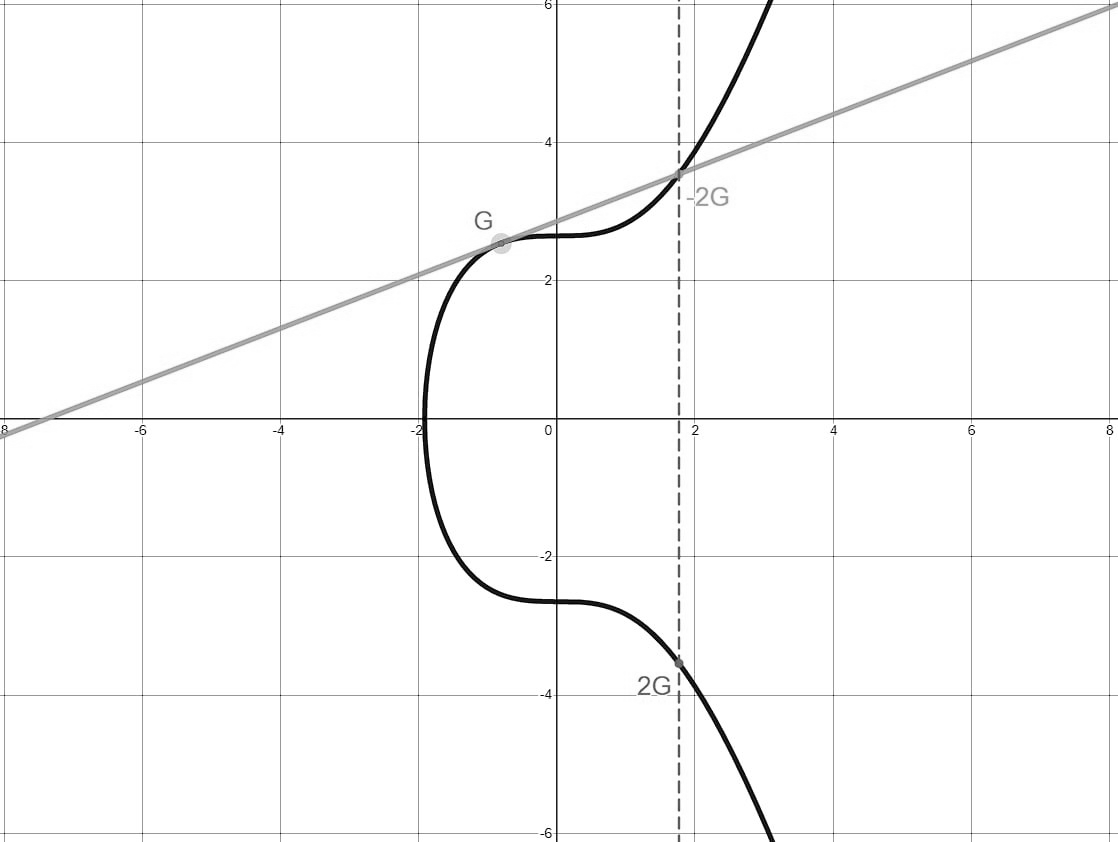
\includegraphics{chapters/img/secp256k1-multiplication.png}

}

\caption{Geometrical representation of doubling point G on secp256k1
(source: Loïc Morel, \emph{Bitcoin Démocratisé}, 2022).}

\end{figure}%

By choosing a private key ( k ), we can calculate the public key ( K )
which is ( K = k\textasciitilde G ). Since multiplication by a scalar is
non-reversible, transitioning from the private key to the public key
constitutes a one-way function. In other words, it is practically
impossible to find the private key from the public key without trying
every possibility one by one.

Let's see what this looks like in practice. The private key is a
randomly chosen number. It must be between ( 1 ) and ( n - 1 ), where (
n ) is the order of point ( G ) (which is close to ( 2\^{}\{256\} )):

\[n = \mathtt{0xfffffffffffffffffffffffffffffffebaaedce6af48a03bbfd25e8cd0364141}\]

For example, the following hexadecimal number is perfectly valid to
serve as a private key:

\[k = \mathtt{0x999bb87eea489b2fc6219226e7b95d9083a3b627246ea852e85567ac4d72444f}\]

The public key is a point on the curve defined by ( K =
k\textasciitilde G ). If we compute this point from the above private
key, we obtain:

\[\begin{aligned}
K = &~(\mathtt{0xf6a6c7c39c88b767bfac4ac687c3ff32372e76c9fb633e2278e54472e300b3bd}, \\
    &~\mathtt{0x5822f24e0fdb4e568f97a7fff246c07ba486c1756f82971765cc9cf8e45ff5e6})
\end{aligned}\]

In Bitcoin, this public key is represented in serialized form. It can be
uncompressed, in which case it is prefixed by \texttt{0x04}. In our
case, its serialized expression is:

\begin{verbatim}
04 f6a6c7c39c88b767bfac4ac687c3ff32372e76c9fb633e2278e54472e300b3bd
5822f24e0fdb4e568f97a7fff246c07ba486c1756f82971765cc9cf8e45ff5e6
\end{verbatim}

There is also a compressed representation of the public key. This is
possible due to the symmetry of the curve with respect to the x-axis:
indeed, the fact that point ( (x, y) ) belongs to the curve implies that
point ( (x, -y) ) also does. To compress the information, it suffices to
provide the abscissa ( x ) and a prefix that is \texttt{0x02} if ( y )
is even or \texttt{0x03} if ( y ) is odd\footnote{In the finite field
  \(\mathbb{F}_p\), taking the opposite of a non-zero element \(y\)
  reverses its parity. Indeed, if \(y \in [\![ 1, p - 1 ]\!]\), then
  \(-y + p \in [\![ 1, p - 1 ]\!]\).}. We can then recover ( y ) using
the curve's equation. In our case, the compressed public key is:

\begin{verbatim}
02 f6a6c7c39c88b767bfac4ac687c3ff32372e76c9fb633e2278e54472e300b3bd
\end{verbatim}

This format reduces the size of transactions (and thus fees), which is
why it is used in most recent wallets and is required in the case of
SegWit. The uncompressed format is thus tending to disappear, although
it remains valid in classic transactions.

In Bitcoin, the public key was initially used to receive funds directly
(``Pay to Public Key''), so it is still sometimes confused with the
notion of an address. However, it is generally its hash obtained through
hashing (``Pay to Public Key Hash'') that serves as the receiving
address, as we will describe below.

The ECDSA signing algorithm applies to a message ( m ) that is
previously hashed and produces a signature ( (r, s) ). It is then
possible to match the signature with the public key ( K ) using a
verification algorithm that does not require knowing the private key ( k
)\footnote{The ECDSA signing algorithm is as follows. Denoting \(H(m)\)
  as the cryptographic hash of the message to be signed, the signature
  is obtained by applying the following steps:}.

In Bitcoin, the message is the transaction. The verification algorithm
thus shows that the person who produced the signature knows ( k ) such
that ( K = k\textasciitilde G ), meaning they are the owner of the
bitcoins. This allows nodes on the network to ensure the validity of
signatures and, consequently, the transaction. An example of a signature
corresponding to our public key and a transaction made on the main
network is\footnote{This is the signature of transaction
  08e5ce0783ab6d5534e234136df02e0e240f76108eb6af04b8b624646b66f5eb. In
  serialized form (DER), this signature is
  3044022019b83a5e354ef62e98413e6ef3f37ad0c69f75cea7daa6a352cf66f4668a9a0b02204c13f9b6f2c8ea7af224b3f6a3d9cfdfe5085bbafa150fb1aa72a20ce7cac6b001.}:

\[\begin{aligned}
(r, s) = &~(\mathtt{0x19b83a5e354ef62e98413e6ef3f37ad0c69f75cea7daa6a352cf66f4668a9a0b}, \\
    &~\mathtt{0x4c13f9b6f2c8ea7af224b3f6a3d9cfdfe5085bbafa150fb1aa72a20ce7cac6b0})
\end{aligned}\]

Note that the ECDSA algorithm presented here is not the only one that
exists. In November 2021, BTC integrated another algorithm---the Schnorr
digital signature scheme---which is based on the same elliptic curve but
offers major benefits. Other Bitcoin variants like Monero use EdDSA, a
signature algorithm based on a twisted Edwards curve.

\section*{Hashing}\label{hashing}
\addcontentsline{toc}{section}{Hashing}

\markright{Hashing}

Bitcoin also makes use of hashing. Hashing is a cryptographic process
that ensures the integrity of digital information. The name of this
process comes from an analogy with cooking, where foods can be chopped
into small pieces and grouped into a hash. It is implemented by a hash
function that transforms a \emph{message} of variable size into a
\emph{hash} of fixed size. This hash is also called a digest or simply a
hash.

Hash functions are deterministic functions that are easily executable
and, in theory, have three characteristics\footnote{These are
  assumptions, and some functions satisfy these characteristics more
  than others. For example, collisions have been found in MD5 and SHA-1
  functions that were thought to be secure.}:

\begin{itemize}
\tightlist
\item
  \textbf{Irreversibility}: They are one-way functions constructed so
  that it is difficult to retrieve the original message from a given
  hash (preimage resistance).
\item
  \textbf{Unpredictability}: Any modification of the original message
  results in a drastically different hash, making it difficult to find a
  similar hash.
\item
  \textbf{Collision resistance}: It is difficult to find two messages
  that result in the same hash.
\end{itemize}

One of the most well-known functions is SHA-256, whose name comes from
``Secure Hash Algorithm'' and the size of the hashes it produces (256
bits, or 32 bytes). For example, if we consider the message ``Bitcoin,''
spelling it in lowercase or adding a period completely changes its hash,
as shown in Table~7.1. This feature notably allows for detecting errors
in the message.

\phantomsection\label{table:sha256-hashes}
\begin{longtable}[]{@{}
  >{\raggedright\arraybackslash}p{(\columnwidth - 2\tabcolsep) * \real{0.5000}}
  >{\raggedright\arraybackslash}p{(\columnwidth - 2\tabcolsep) * \real{0.5000}}@{}}
\toprule\noalign{}
\begin{minipage}[b]{\linewidth}\raggedright
\textbf{Message}
\end{minipage} & \begin{minipage}[b]{\linewidth}\raggedright
\textbf{Hash (SHA-256)}
\end{minipage} \\
\midrule\noalign{}
\endhead
\bottomrule\noalign{}
\endlastfoot
Bitcoin &
b4056df6691f8dc72e56302ddad345d65fead3ead9299609a826e2344eb63aa4 \\
bitcoin &
6b88c087247aa2f07ee1c5956b8e1a9f4c7f892a70e324f1bb3d161e05ca107b \\
Bitcoin. &
a9adf3c04d168153b296083f05015f587d7df6e0b85305b6c7beb2a69e3f4e75 \\
\end{longtable}

\emph{Hashes by SHA-256 of slightly different messages.}

Hashing is involved in multiple areas within Bitcoin: in the signing
algorithm (message hashing), in calculating addresses, in key
derivation, for computing checksums, for calculating transaction and
block identifiers, in constructing Merkle trees in blocks, and finally
at the core of mining.

Three hash functions are used: SHA-256, which produces 256-bit (32-byte)
hashes; RIPEMD-160, whose name stands for ``RACE Integrity Primitives
Evaluation Message Digest'' and results in 160-bit digests; and SHA-512,
which hashes data into 512-bit hashes.

The most frequently used function is double SHA-256 (noted SHA-256d or
HASH-256), which appears almost everywhere. It is supposed that this
doubling implemented by Satoshi was intended to protect against length
extension attacks. The composition of SHA-256 with RIPEMD-160 is used
for calculating addresses. This is the only substantial use of
RIPEMD-160\footnote{``Bitcoin addresses are the only place where 160-bit
  hashing is used.'' --- Satoshi Nakamoto, \emph{Re: Stealing Coins},
  07/25/2010 20:48:01 UTC:
  \url{https://bitcointalk.org/index.php?topic=571.msg5754\#msg5754}.}.
Finally, SHA-512 is used in the key derivation algorithm implemented in
wallets.

\section*{Private Keys}\label{private-keys}
\addcontentsline{toc}{section}{Private Keys}

\markright{Private Keys}

Essentially, a private key is digital information---that is, a number.
More precisely, it is a very large number between ( 1 ) and ( n-1 ),
where ( n ) is the order of point ( G ) and approaches ( 2\^{}\{256\} ),
approximately ( 1.1579 \times 10\^{}\{77\} ). The interval is
exceedingly vast, making it statistically impossible to stumble upon the
same private key by choosing at random. For comparison, the number of
atoms in the observable universe is close to ( 10\^{}\{80\} ).

The private key is randomly created, most often using pseudo-random
number generator algorithms that aim to reproduce randomness as
faithfully as possible in computing. This generation relies on the
device's computational entropy---that is, the amount of randomness it
collects through hardware sources (variance of fan or hard drive noise)
or external sources (mouse movement, keyboard signals, etc.). Tools used
to generate private keys are usually considered cryptographically secure
(CSPRNG).

The randomness of the process is fundamental, forming the basis of the
model's security. For example, someone who chooses the number 1 as a
private key could never use the corresponding address, as the security
linked to this key is nil. All bitcoins deposited to this address would
be instantly debited by a specialized program\footnote{One can observe
  the address 1EHNa6Q4Jz2uvNExL497mE43ikXhwF6kZm (corresponding to key
  1) to be convinced that this is not a good choice.}.

The same goes for ``brain wallets,'' which rely on memorizing
information and are often created insecurely. People typically start
with a coherent phrase (like a quote from a book or song) to make it
easy to remember, then hash it and use the resulting hash as a private
key. This practice is highly risky due to the strong predictability of
human language, and addresses created this way are likely to be emptied,
as shown in a BitMEX Research investigation\footnote{BitMEX Research,
  \emph{Call me Ishmael}, October 13, 2020:
  \url{https://blog.bitmex.com/call-me-ishmael/}.}.

This importance of randomness is also reflected in the ECDSA algorithm,
which relies on generating an ephemeral key to produce the signature. If
this value is not correctly generated, an attacker could deduce private
keys from signatures. This is what happened in August 2013 when a
vulnerability (CVE-2013-7372) was discovered within Java's SecureRandom
function, affecting the security of several Android software
wallets\footnote{Bitcoin.org, \emph{Android Security Vulnerability},
  August 11, 2013:
  \url{https://bitcoin.org/en/alert/2013-08-11-android}.}. Exploiting
this flaw led to the loss of at least 55.82 bitcoins, about \$5,200 at
the time.

After being generated, private keys must then be encoded to facilitate
their transmission for import into a wallet or export. In Bitcoin, they
are represented using the Base58Check encoding. This is why we sometimes
refer to the Wallet Import Format (WIF).

Encoding a key follows a series of simple steps. First, the key is
prefixed with the version byte \texttt{0x80}, indicating that it is a
private key. Then, a suffix \texttt{0x01} is added (or not) to indicate
whether we want to derive a compressed (or uncompressed) public key. In
the case of our example key, we obtain the following bytes:

\begin{verbatim}
80 999bb87eea489b2fc6219226e7b95d9083a3b627246ea852e85567ac4d72444f 01
\end{verbatim}

Next, the checksum is calculated by taking the first 4 bytes of the
double SHA-256 hash and added after the set:

\begin{verbatim}
80 999bb87eea489b2fc6219226e7b95d9083a3b627246ea852e85567ac4d72444f 01
1dd28791
\end{verbatim}

Finally, the whole is encoded in base 58. In the ``compressed'' case,
the key always starts with a K or an L. Here, our private key is
written:

\begin{verbatim}
L2NJfKog9SEdoAkAkm8ZNYDcpWQop95orPepbhsTE2t5Bf1yFmYk
\end{verbatim}

In the ``uncompressed'' case (less commonly used), the key always starts
with a 5. Here, our private key becomes:

\begin{verbatim}
5JywJHwyuD4YSsErniGJkrDNi87kggSZNADCEkhRyRScqfMMTEt
\end{verbatim}

\section*{Addresses}\label{addresses}
\addcontentsline{toc}{section}{Addresses}

\markright{Addresses}

In Bitcoin, an address is essentially an account number used to receive
funds. This data is publicly available on the blockchain, and anyone can
verify its balance. However, a user can generate as many addresses as
they wish to avoid revealing all their activity.

Generally, an address is the hash of a public key (PKH), the public key
itself (PK), or the hash of a script (SH). Here, we will discuss simple
addresses derived from public keys through hashing, which are the most
used on the BTC network.

A simple address is obtained by successively hashing the serialized
public key using the SHA-256 and RIPEMD-160 functions. The composition
of these two functions is commonly called HASH-160. RIPEMD-160 was
chosen by Satoshi to shorten the length of addresses, as it produced
20-byte hashes instead of the 64 bytes of a public key or the 32 bytes
produced by SHA-256. Denoting ( A ) as the address, we have:

\[A = \text{HASH160}(K) = \text{RIPEMD160}(\text{SHA256}(K))\]

Since this composition is itself a hash function, it also has the
characteristic of being a one-way function. Therefore, it is virtually
impossible to retrieve the public key from the address.

The risk of collision is also statistically nil, even though there are
fewer addresses than private keys. The RIPEMD-160 hash function produces
160-bit hashes, resulting in ( 2\^{}\{160\} ) (approximately ( 1.4615
\times 10\^{}\{48\} )) possible addresses, which is roughly ( 8
\times 10\^{}\{28\} ) times fewer addresses than private keys. However,
this number is sufficiently large that the risk of randomly landing on
the same address is completely negligible\footnote{Suppose a global
  population of 10 billion humans uses Bitcoin actively, with each
  individual generating 1 million addresses on average. The probability
  of a collision would then be:
  \[10^{16} / 2^{160} \approx 0.000000000000000000000000000000684\%.\]
  Even if an individual attempted to build a specialized machine
  generating and checking a trillion (( 10\^{}\{18\} )) addresses per
  second operating continuously, the probability of accessing an already
  used address would still be negligible (on the order of (
  10\^{}\{-21\} )). Our brains are not wired to comprehend such numbers.}.

Since a public key has two serialized representations (compressed and
uncompressed), it is possible to calculate two hashes. Here, we focus on
the compressed representation. The hash of our compressed public key is:

\begin{verbatim}
a18bd7f41b42c7cc6ebfa4de43e6b63248536ebc
\end{verbatim}

From this, we can derive three different types of addresses: a legacy
address, a native SegWit address, and a nested SegWit address. In all
three cases, the principle is the same, although the specific use of the
hash in the protocol differs.

The legacy address is obtained by encoding the hash in Base58Check with
the version byte \texttt{0x00}. Due to this version byte, simple legacy
addresses always start with a 1 (purely symbolic since it equals 0 in
base 58). Our address is:

\begin{verbatim}
1FjBKPQ7MTiPSDkJ2ZwPgAXUKQ8yoGbVJX
\end{verbatim}

This type of address is called P2PKH (Pay to Public Key Hash) and was
the first type of address in Bitcoin.

The native SegWit address is encoded using the Bech32 format. This
includes a prefix indicating the network (\texttt{bc} for BTC) and a
separator (\texttt{1}). Similar to the encoding of legacy addresses, it
involves taking the raw information (``payload''), prefixing it with the
SegWit version byte (\texttt{0x00} for the first version of SegWit),
calculating a checksum, and expressing the whole in the appropriate
base, namely base 32. This process results in the address always
starting with \texttt{bc1q}. In the case of our public key hash, we
obtain:

\begin{verbatim}
bc1q5x9a0aqmgtrucm4l5n0y8e4kxfy9xm4udhygr2
\end{verbatim}

This type of address is called P2WPKH (Pay to Witness Public Key Hash).

Finally, we can also include this data in the form of a script in a P2SH
address, creating a so-called ``nested'' SegWit address. The script,
composed of the SegWit version byte (\texttt{0x00}) and the hash, is
hashed to form the new address. As with all P2SH addresses, the
resulting hash is encoded in Base58Check with the version byte
\texttt{0x05}. This version byte causes the address to start with a 3.
Our hash becomes:

\begin{verbatim}
3JqPHkGuvW7nsUJDgm5CPSNUb47WczCC5e
\end{verbatim}

This type of address is called P2SH-P2WPKH (P2SH-nested Pay to Witness
Public Key Hash). We will discuss in more detail the different script
schemes underlying these address types in Chapter~12.

Once encoded, addresses can be easily shared from one person to another.
Thanks to the checksum, a typo theoretically poses no risk, as the
software will detect it and refuse to proceed with the payment.
Addresses are also often represented by QR codes (see Figure~7.3),
better suited for interaction with smartphones.

\begin{figure}

{\centering 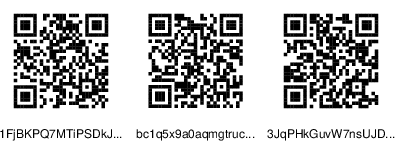
\includegraphics{chapters/img/address-qr-codes.png}

}

\caption{QR codes of addresses.}

\end{figure}%

In summary: when a user wants to receive a payment, they generate a
private key, derive a public key from it, and create an address from the
public key; they share their address with another user who sends them
funds; they can then spend the received funds by signing a transaction
using their private key. The Bitcoin peer-to-peer network then verifies
that the signature matches the public key.

The public key is only revealed to the network during the transaction.
This implies that funds are protected against the possibility of a
faulty implementation of the signature algorithm (as in the case of
exploiting the vulnerability within SecureRandom in 2013) or the
generalized compromise of ECDSA (by a quantum computer, for example).
This is a secondary benefit of using new addresses for each payment.

Beyond BTC, other cryptocurrencies have their own encoding for
addresses, often a variant of the standard modifying the version or
prefix. Thus, in Litecoin, legacy addresses start with an \texttt{L}
(e.g., LZx8abhwS7xSh2STChvgxBbEXcWG1AZ2iR), and SegWit addresses start
with \texttt{ltc1q} (e.g., ltc1q5x9a0aqmgtrucm4l5n0y8e4kxfy9xm4uft7vm6).

Bitcoin Cash also has its own address format, called CashAddr, which is
heavily inspired by the Bech32 format. This format was introduced to
differentiate BTC addresses from BCH addresses. A BCH address is simply
an alternative representation of the P2PKH type: in this format, the
address 1FjBKPQ7MTiPSDkJ2ZwPgAXUKQ8yoGbVJX becomes
bitcoincash:qzsch4l5rdpv0nrwh7jduslxkceys5mwhs03g7e6dq.

\section*{Wallets}\label{wallets}
\addcontentsline{toc}{section}{Wallets}

\markright{Wallets}

A wallet is a method of storing private keys that grant access to a
user's cryptocurrency funds. This method is often combined with
cryptocurrency management: receiving it by reading the blockchain and
sending it by producing signatures. The medium used can be a simple
piece of paper or a computer file, but it is generally software on a
mobile device or computer, or a specialized device.

A wallet is essentially a \emph{keychain}. Its main role is to securely
store private keys over time to guarantee ownership of bitcoins. Most of
the time, keys are deterministically generated by these wallets from a
12- to 24-word recovery phrase. The user must therefore carefully
preserve this phrase on another medium to recover their funds if their
device is lost, broken, or stolen.

However, an account with a custodian like a centralized exchange is not
truly a wallet because these services hold their users' private keys for
security and ease of use. Thus, applications that closely resemble
wallets, like the Wallet of Satoshi or the Coinbase app, are not.

We can classify existing wallets into two main categories: ``hot
wallets'' that are connected to the Internet during use, and ``cold
wallets'' that are never directly connected. Additionally, within these
two categories, there are different types of wallets, each with its own
strengths and weaknesses.

Hot storage of private keys, which uses devices directly connected to
the Internet, includes software wallets that can be installed on a
mobile device, tablet, or general-purpose computer. These software
applications usually make their source code available to the public for
obvious security reasons. Keys are stored on the computer and are
generally encrypted. This category includes full node software,
lightweight wallets, browser extensions, and web wallets.

A full node implementation, also called a full client, is the first type
of wallet that appeared and the only one that existed during Satoshi's
time. As its name suggests, such software performs all the operations
necessary to maintain a node on the peer-to-peer network: it downloads
the entire blockchain and verifies and relays unconfirmed transactions
and blocks. Bitcoin Core is the most well-known full node software.
However, due to its difficulty of use, this type of wallet is generally
no longer used directly; novices prefer lighter applications, and
advanced users favor more secure solutions that they can connect to
their personal node if they wish.

A lightweight wallet, also known as an SPV wallet (for Simplified
Payment Verification), is software that does not download the blockchain
but performs simplified transaction verification using the chain of
headers, requiring few computing resources. This type of wallet is
particularly suited to small devices like phones. The software can
interact with all the full nodes in the peer-to-peer network, as BRD
(formerly breadwallet) does, but generally goes through dedicated server
infrastructure to make usage more pleasant, as is the case with Electrum
or Sparrow. This type of wallet ensures the safety of funds but can have
a detrimental effect in other areas, particularly regarding privacy. The
user can also choose to connect their wallet to their own full node.

A wallet can also take the form of a browser extension, whether on
Chrome, Firefox, or Brave. Unlike lightweight clients, these wallets do
not always perform transaction verification and trust the server they
are connected to.

Finally, the last type of hot storage is the web wallet. These are
online interfaces that allow users to manage funds. Unlike exchanges,
the user retains control of their private keys when using this kind of
service: the keys are managed by the browser and are never revealed to
others. The most well-known wallet of this type is Blockchain.com's
wallet.

But these hot solutions are not the only ones, and there are methods of
cold storage for private keys that are completely disconnected from the
Internet. This storage method has the merit of reducing the attack
surface and thus the risk of theft through hacking. It is the
recommended solution for securing large amounts of cryptocurrency.

Ideally, you need a device that remains constantly offline to generate
keys and addresses. This device can be an old computer not connected to
the Internet or specialized hardware. The two main methods for cold
storage are paper wallets and hardware wallets.

A paper wallet is the simplest type of wallet imaginable: private keys
generated offline (and their corresponding addresses) are written on a
piece of paper. The information can also be a mnemonic phrase. The paper
wallet has a major drawback: the inability to sign transactions without
importing it into an online interface. This method is not practical at
all because the user cannot sign transactions without compromising the
security of their wallet and must be content with receiving payments. To
solve this problem, hardware wallets exist.

A hardware wallet is a device specifically designed to generate and
securely store private keys and allow transactions to be signed offline.
It is currently the safest way to hold bitcoin. These wallets are built
so that someone who gets hold of them cannot spend the funds without the
user's password.

There is a variety of hardware wallets. The best-known are those from
Satoshi Labs (the Trezor One and Trezor Model T) and those from Ledger
(the Nano S and Nano X), which are the oldest and most recognized
models. These can be safely connected to a computer, and transactions
are always signed on the device. Some others enhance security by being
physically isolated from any third-party computer (using an air gap),
like the Coldcard Mk4. Other wallets focus on ease of use, such as
Satochip cards that are based on smartcards.

All wallets involve a certain level of trust: you must rely on the
software you use to store your bitcoins, the program you use to generate
a paper wallet, or the hardware specialized in cold storage. Of course,
open-source solutions can be considered safer in the sense that people
other than the designers have been able to verify the final product,
which is notably the case for many software wallets and the hardware
infrastructure of Trezor wallets. In any case, a component based on
reputation remains.

In general, each type of wallet has its utility: it's up to the user to
determine which wallet best suits their needs.

\section*{Key Derivation}\label{key-derivation}
\addcontentsline{toc}{section}{Key Derivation}

\markright{Key Derivation}

During Bitcoin's early days, private keys were randomly generated by the
software each time it was used. Consequently, the keys were stored in a
file called \texttt{wallet.dat} on the computer's hard drive. This made
key loss more likely.

However, modern wallets no longer work this way. Keys and addresses are
deterministically derived from a single randomly generated piece of
information, which takes the form of a mnemonic phrase ranging from 12
to 24 words. These words can be in English, French, or another language.

\emph{elder process crowd gentle proof taxi bean patient around warm
source boil}

Therefore, preserving this phrase, called a recovery phrase, ensures the
security of the bitcoins. This phrase allows you to recover your funds
if your device is stolen or broken. That's why it must remain secret.

This type of wallet is sometimes called an HD wallet for Hierarchical
Deterministic Wallet. The concept was developed for Bitcoin starting in
2011. It was standardized in 2012 within BIP-32 written by Pieter Wuille
and proposals BIP-39 and BIP-44 written by Marek Palatinus and Pavol
Rusnak. It was expanded to other cryptocurrencies in 2014.

Generally, the secret phrase or recovery phrase is generated by the
user's device, whether it's a mobile phone, computer, or hardware
wallet. To do this, entropy is first created by the device in a
pseudo-random manner. The information, which has a specific number of
bits, is then enriched with a checksum of a few bits, allowing errors in
input to be detected, and the whole is divided into 11-bit segments.
Finally, each of these segments is associated with a word from the
standard list of 2048 words, forming the phrase. This derivation is
illustrated in Figure~7.4.

The number of words in the phrase depends on the desired entropy size.
Thus, 128 bits of entropy is equipped with a 4-bit checksum, resulting
in a 12-word phrase of 11 bits each. For 256 bits, there is an 8-bit
checksum and thus a 24-word phrase.

\begin{figure}

{\centering 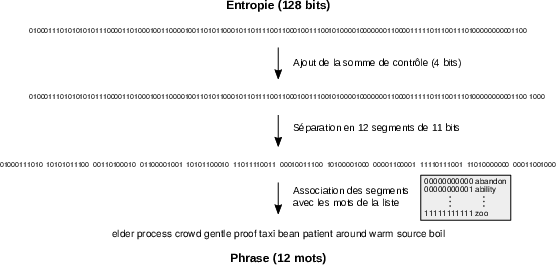
\includegraphics{chapters/img/from-entropy-to-mnemonic.png}

}

\caption{From entropy to the mnemonic phrase.}

\end{figure}%

Various cryptographic processes are used to derive keys and addresses
from this phrase. These derivation processes have similar properties to
hash functions, producing irreversible, unpredictable, and
collision-resistant results.

The first is the HMAC-SHA512 message authentication code (HMAC stands
for Hash-Based Message Authentication Code), which calculates a hash
using the SHA-512 hash function in combination with a secret key. The
second is the PBKDF2 key derivation function (Password-Based Key
Derivation Function 2), which repeatedly applies a function chosen by
the user to a message of arbitrary size with a cryptographic salt. The
advantage is that it requires a significant amount of computation to
prevent brute-force cracking of the higher-level information.

In Bitcoin, PBKDF2 is used to derive a seed from the mnemonic phrase by
applying the HMAC-SHA512 function 2048 times. The cryptographic salt is
the term \texttt{mnemonic} to which a passphrase can be added to enhance
security. The resulting seed is 512 bits (64 bytes) of information, from
which the master key and subsequent keys are derived.

Key derivation is done using the HMAC-SHA512 algorithm. First, an
initial derivation is performed from the seed. The HMAC is applied to
the seed and the cryptographic salt \texttt{Bitcoin\ seed}, yielding a
master key (first 256 bits of the result) and a master chain code (last
256 bits of the result). The transition from the secret phrase to the
master private key and master chain code is summarized in Figure~7.5.

\begin{figure}

{\centering 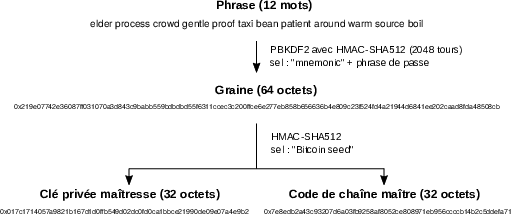
\includegraphics{chapters/img/from-mnemonic-to-root.png}

}

\caption{From the mnemonic phrase to the master key.}

\end{figure}%

These two pieces of information allow all subsequent derivations to be
made. The chain code is used in the key derivation chain so that it's
impossible to perform the derivation without it.

Rather than managing these two pieces of information separately, it's
preferable to use extended private keys, which include the private key
and chain code, as well as other information like the depth and index of
the child key. The extended private key is encoded in Base58Check with a
special prefix that depends on the type of address derived, resulting in
the key starting with \texttt{xprv} (legacy addresses and Taproot keys),
\texttt{yprv} (nested SegWit addresses), or \texttt{zprv} (native SegWit
addresses). In our case, the extended private key derived from the
master private key and master chain code is:

\begin{verbatim}
xprv9s21ZrQH143K3KSN1mSK8myNuDcXNvNoCDcU4KBxMTuj1Wo83zNn
jaj8dKFT81GttcgPftdB4XhAzzQLXJEGDtFp35yssYnxDV3yVDEqv1b
\end{verbatim}

Similarly, the extended public key groups the public key and the chain
code corresponding to the private key from which it is derived. In
Base58Check, this key always starts with \texttt{xpub}, \texttt{ypub},
or \texttt{zpub}. The extended public key corresponding to the master
private key is:

\begin{verbatim}
xpub661MyMwAqRbcFoWq7nyKVuv7TFT1nP6eZSY4rhbZuoShtK8GbXh3
HP3cUapsPsqEd52TRk1vhkgkhtAReezgSBi4ELh3YoxjmZgKBk7U98h
\end{verbatim}

Child key derivation involves using the HMAC-SHA512 algorithm to derive
``child'' extended keys from a ``parent'' extended key. Chain codes are
used as the cryptographic salt. There are two types of derivation:
normal derivation and hardened derivation.

Normal derivation involves the extended public key in the process,
allowing two operations: obtaining the child extended public key from
the parent extended public key, and obtaining the child extended private
key from the parent extended private key. The functioning of this type
of derivation is illustrated in Figure~7.6.

\begin{figure}

{\centering 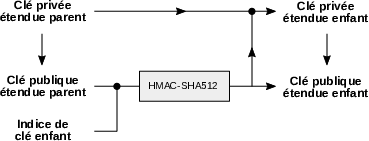
\includegraphics{chapters/img/normal-child-key-derivation.png}

}

\caption{Normal key derivation using HMAC-SHA512.}

\end{figure}%

This feature of derivation is extremely useful for generating new
addresses without compromising the root private key. A user can thus
import the extended public key into a payment processor to verify their
balance and generate new addresses without providing the private key. It
also allows merchants to have employees receive payments at different
addresses without worrying about fund security.

However, this feature poses a potential risk: if a child private key is
disclosed, knowledge of the parent extended public key (and thus the
corresponding chain code) allows one to obtain all child private keys as
well as the parent private key.

That's why there is a second type of derivation: hardened derivation,
which, unlike the first, is restricted to the calculation of child
(extended) private keys, ensuring better security. This is depicted in
Figure~7.7.

\begin{figure}

{\centering 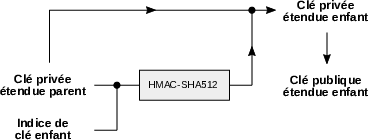
\includegraphics{chapters/img/hardened-child-key-derivation.png}

}

\caption{Hardened key derivation using HMAC-SHA512.}

\end{figure}%

Each derivation involves an index, encoded on 32 bits as a signed
integer, where the sign bit indicates whether it should be hardened or
not, and the value indicates the child key's number. Thus, one can
produce 2,147,483,648 (( 0 ) to ( 2\^{}\{31\} - 1 )) normal child keys
and 2,147,483,648 hardened child keys (( -0 ) to ( -2\^{}\{31\} + 1 ))
from the same parent key.

Conventionally, an apostrophe is used to denote this sign\footnote{Sometimes
  the letter \texttt{h} (for \emph{hardened}) is used.}. The index
\texttt{2} indicates the third normal child key. The index \texttt{44’}
indicates the 45th hardened child key.

Successive derivations allow for the creation of derivation trees, where
the position of each key can be found using a path---the derivation
path. This is typically started with the letter \texttt{m} to indicate
that we're starting from the master private key. An example of a
derivation path is m/84'/0'/0'/1/17.

Each wallet can use its own derivation path. However, a standard has
emerged---BIP-44. This simplifies the construction of multi-purpose
wallets supporting multiple cryptocurrencies and allowing multiple
accounts for each\footnote{Not all wallets adhere to this standard. The
  BRD wallet (formerly Breadwallet), for instance, uses the path
  \texttt{m/0’} to derive the main account, following the initial
  recommendations of BIP-32.}.

In this standard, three hardened derivations are performed, followed by
two normal derivations, to arrive at a private key and its corresponding
address. Each derivation provides information:

\begin{itemize}
\tightlist
\item
  The first derivation (hardened) defines the wallet's purpose: 44
  (referring to BIP-44) allows for deriving an account using legacy
  addresses, 49 (BIP-49) for nested SegWit addresses, 84 (BIP-84) for
  native SegWit addresses, 48 or 45 (BIP-45) for multisignature
  addresses, 86 (BIP-86) for deriving public keys related to Taproot,
  etc.
\item
  The second derivation (hardened) indicates the crypto-economic
  protocol and, by extension, the associated unit of account: the number
  0 is used for BTC, 1 for the testnet, 2 for LTC, 60 for ETH, 128 for
  XMR, 145 for BCH, etc.
\item
  The third derivation (hardened) gives the account index: 0, 1, 2, etc.
\item
  The fourth derivation (normal) indicates the address role: 0 signifies
  an external address, used to receive bitcoins; 1 signifies an internal
  address, used to receive change when sending bitcoins (a phenomenon
  we'll describe in Chapter~12).
\item
  The fifth derivation (normal) gives the key and address index: 0, 1,
  2, etc.
\end{itemize}

Thus, the derivation path looks like this:

\begin{verbatim}
m / purpose' / protocol' / account' / address_role / address_index
\end{verbatim}

For example, the key m/44'/0'/0'/0/0 corresponds to the first receiving
address of a Bitcoin account using legacy addresses. Similarly, the key
m/84'/0'/0'/1/17 corresponds to the 18th change address of the first
Bitcoin account using native SegWit addresses.

All addresses of a wallet remain valid even if they have been used.
Although one can generate infinite addresses, the wallet usually scans
20 addresses from the last active address.

\section*{Property in Bitcoin}\label{property-in-bitcoin}
\addcontentsline{toc}{section}{Property in Bitcoin}

\markright{Property in Bitcoin}

Property is the absolute control exercised over a good by a person to
the exclusion of all others. Often, property is exercised through a
property right that legally establishes the power dynamics. The owned
good can be a book, a car, or land.

Property is fundamental to money: without real control over monetary
units, exchange is impossible. Indeed, the transfer of precious metal
coins or fiduciary banknotes requires that the holder fully controls
them and can relinquish them at the time of the transaction. That's why
we also talk about \emph{liquid} cash.

Without this property, the characteristics of money crumble. Today, most
transactions involve the exchange of bank credit, whether through card
payments, transfers, or other digital means. This situation exposes
people increasingly to forms of censorship resulting from regulatory
constraints and banking arbitrariness, such as prohibitions on sending
transfers or freezing accounts without notice, in addition to the bank's
solvency risk.

Bitcoin allows individuals to fully own their money while retaining the
digital and immaterial aspects of its use. This property is different
from that exercised over objects: it is indeed inseparable from the
exclusive knowledge of information (the private keys) and the protection
of that information.

Thus, information is more valuable than ever. We've always associated
value with knowledge due to the power it brings (\emph{scientia potentia
est}), but this value was indirect. Today, information can provide
direct access to a certain amount of cryptocurrency: if someone knows
the private key corresponding to an address containing bitcoins, they
\emph{de facto} own those bitcoins.

A user can hold bitcoin extremely easily by memorizing the private key
or recovery phrase. They can, for example, cross a state border
possessing a piece of paper with the information, or simply keep it in
mind. This is exemplified by a German criminal who, after fraudulently
mining 1,700 bitcoins by installing software on computers without their
owners' knowledge, was able to keep his fortune despite his two-year
imprisonment\footnote{Clément Wardzala, ``\emph{Bitcoin: the German
  police searching for a \$65 million password}'', \emph{Cryptoast},
  February 5, 2021:
  \url{https://cryptoast.fr/bitcoin-police-allemande-recherche-mot-de-passe-65m/}.}.

A user can receive bitcoins by generating a new private key on a device.
No authorization from the network is required, although they must, of
course, have Internet access to verify incoming payments. Due to the
system's resistance to censorship, they can do whatever they want with
their bitcoins: fund sensitive causes, buy drugs on the dark web, gamble
online, send funds abroad, etc. There is no limit on the amount,
providing a wealthy individual with a means to have a much greater
impact on the world.

\section*{Custody Risk}\label{custody-risk}
\addcontentsline{toc}{section}{Custody Risk}

\markright{Custody Risk}

Even though Bitcoin enables free exchange through cyberspace, it hasn't
eliminated trusted third parties. Indeed, many people lack confidence in
their ability to store their bitcoins themselves and prefer to delegate
this responsibility to custodial services, such as specialized
custodians, online marketplaces, or payment apps. It's also more
convenient to use a bank to lend money and make it grow, which benefits
online lending platforms.

While this behavior is understandable, it's important to emphasize that
those who save bitcoins through a custodian do not actually own those
bitcoins. The claim they have on the trusted third party is not
ownership of the bitcoins since the custodian holds them. State law may
intervene, but that doesn't prevent this real control from manifesting
in various cases. This is the meaning of the adage ``not your keys, not
your coins,'' popularized by Andreas Antonopoulos\footnote{Andreas
  Antonopoulos, \emph{Bitcoin Q\&A: How Do I Secure My Bitcoin?}
  (video), July 7, 2017:
  \url{https://www.youtube.com/watch?v=vt-zXEsJ61U}.}, reminding us that
those who do not manage their private keys themselves do not truly own
the bitcoins they believe they possess.

While delegating property offers certain advantages, it also has
drawbacks and poses risks to those who do so. First, custodians can go
bankrupt if their reserves become too low for withdrawal requests. In
case of bankruptcy, the client does not recover all their funds unless
another entity absorbs the platform's losses.

First, this bankruptcy can materialize following a loss of funds, as
happened in July 2011 to the Polish exchange Bitomat, which lost the
private keys linked to 17,000 BTC due to a technical incident.

Second, it can result from external theft, such as hacking. The most
well-known example is the Mt. Gox exchange, which experienced multiple
hacks between 2011 and 2013 leading to the disappearance of 650,000
bitcoins and went bankrupt in 2014. Creditors' debts (in dollars) from
the platform are expected to be repaid in 2024, ten years after the
events.

Third, this bankruptcy can result from an exit scam or internal theft,
where the platform manager ``runs off with the cash.'' This type of
incident was illustrated in July 2011 by the closure of the MyBitcoin
service after the supposed theft of 78,740 BTC by its anonymous founder,
Tom Williams. Another case is the Canadian exchange QuadrigaCX, which
went bankrupt in 2019 following the death of its founder and CEO, Gerald
Cotten, who turned out to have spent the funds to finance his lifestyle
and addiction to speculation. The bankruptcy of the popular exchange FTX
in November 2022, following the fraudulent use of its clients' funds, is
another explosive example of this type of event.

Fourth, even if no loss or theft of funds occurs, fractional reserve
operations by the custodian can push it into bankruptcy due to a credit
tightening. This notably happened to lending platforms Celsius, Three
Arrows Capital, Voyager Digital, BlockFi, and Genesis Files in
2022--2023.

Furthermore, besides the risk of bankruptcy, using a custodian carries
the risk of state intervention. The platform, provided it operates in
the legal market, complies with various AML/CFT regulations and may
therefore be required to freeze an account or even seize the funds it
holds. This is what Coinbase did on March 7, 2022, by blocking 25,000
addresses in the context of Western sanctions against Russia\footnote{Paul
  Grewal, \emph{Using Crypto Tech to Promote Sanctions Compliance},
  March 7, 2022:
  \url{https://blog.coinbase.com/using-crypto-tech-to-promote-sanctions-compliance-8a17b1dabd68}.}.
The platform can also be shut down by authorities, as was the case with
BTC-e in July 2017, which was seized by the U.S. Department of
Justice\footnote{Department of Justice, \emph{Russian National And
  Bitcoin Exchange Charged In 21-Count Indictment For Operating Alleged
  International Money Laundering Scheme And Allegedly Laundering Funds
  From Hack Of Mt. Gox}, July 26, 2017:
  \url{https://www.justice.gov/usao-ndca/pr/russian-national-and-bitcoin-exchange-charged-21-count-indictment-operating-alleged}.}.

Finally, another drawback of using a custodian is the case of forks,
which are permanent duplications of the blockchain creating two distinct
currencies, and airdrops, which are free token distributions for
advertising purposes. In both cases, the user's address is credited with
an additional asset that becomes their property. However, if the person
goes through a custodian, the latter may choose not to transfer it to
them, generally in a non-fraudulent manner, according to the criteria
determined by the terms of use upon registration. Regarding forks, one
can cite the example of the Bitstamp exchange, which refused to cede its
users' Bitcoin SV after the split between BCH and BSV in November 2018
and continues to hold them\footnote{Patrick Thompson, ``\emph{Crypto
  exchanges delisting, denying access and stealing BSV}'',
  \emph{CoinGeek}, January 17, 2020:
  \url{https://coingeek.com/crypto-exchanges-delisting-denying-access-and-stealing-bsv/}.}.
For airdrops, one can mention the case of HEX, an open Ponzi scheme,
whose genesis in 2020 was partly determined by the possession of
bitcoins: each bitcoin holder could claim an amount of HEX tokens
proportional by publishing a digital signature on the Ethereum chain,
but it seems that no platform took the risk of benefiting from this
airdrop.

The non-distribution of the fruits of forks and airdrops thus represents
a loss or at least a missed gain for the client, especially if it's a
split between two economies of equivalent size. However, nothing can
force a custodian to offer the withdrawal of these gains, as the
technical implementation has a significant cost. Conversely, platforms
would be forced to support all such creations, including the most
fanciful ones, like the opportunistic forks of BTC that took place in
2017--2018 (Bitcoin Gold, Bitcoin Diamond, Bitcoin Private, etc.)

In general, relying on custodians has major drawbacks, meaning that the
user does not benefit from Bitcoin's resistance to censorship and
inflation. Holding bitcoin on regulated platforms only allows them to
enjoy the state's temporary leniency regarding the transfers made and
the realized capital gains. Moreover, the widespread custody of funds
presents a systemic risk, as we will see. Therefore, resorting to
custodians should be considered the exception rather than the rule when
it comes to storing bitcoins.

\section*{Property and
Responsibility}\label{property-and-responsibility}
\addcontentsline{toc}{section}{Property and Responsibility}

\markright{Property and Responsibility}

While Bitcoin allows users to own their money sovereignly, this
ownership comes with responsibility. This user must understand how the
system works, at least rudimentarily. They must choose which software
and hardware to use. They must handle funds, verify addresses, and
remain vigilant at all times. In the case of a fork without replay
protection, they must themselves separate the coins on both sides. They
are alone in the face of uncertainty and, above all, themselves. This
responsibility is the price to pay for monetary freedom.

It's understandable that some people lacking technical knowledge end up
delegating this management, especially to speculate. However, the
primary interest of Bitcoin is not to return to a banking system: it's
to fully own one's funds without them being frozen by a trusted third
party or diluted by monetary inflation.

Since securing bitcoins is based on the knowledge of information,
holding bitcoins is inextricably linked to the dilemma between data loss
and data leakage. To keep their bitcoins, one must both maintain access
to their private keys (avoid data loss) and exclude others from them
(avoid data leakage), which can never be fully achieved.

This dilemma can only be resolved through a compromise between security
against loss and security against theft, which is unique to each person.
For example, someone might simply memorize their 12 or 24 words to hold
their bitcoins, at the risk of forgetting them and losing them forever.
Conversely, another person might keep multiple backups in different
places, at the risk of a third party accessing one of them and seizing
their funds.

On one side, we have bitcoin theft. This can occur through burglary:
someone breaks into a home and takes the physical medium containing the
backup or password. But it can also be carried out through intimidation:
owners are physically attacked to be extorted. Hal Finney's family, for
instance, was targeted by a blackmailer who had them swatted by
convincing special police units to intervene urgently at the family
home.

There are best practices to avoid exposure to such theft. First, it's
essential to preserve confidentiality by avoiding declaring that you own
cryptocurrencies, how much you own, for how long, etc. This advice also
applies to exchanges, which know their clients' identities and their
withdrawal addresses and may disclose this information following a state
request or a leak.

Then, the user can improve their storage. They can avoid keeping backups
in the most sensitive places (like their home). They can also distribute
funds across wallets managed differently to mitigate the impact of
theft, although this also increases the risk of such theft occurring.

It's also possible to set up a secondary hidden account within a
hardware wallet by exploiting the use of a passphrase. This is a feature
that Ledger integrates into its products. This technique has the merit
of creating ``plausible deniability'' to present to an assailant who
threatens or tortures the holder.

Finally, one can make bitcoin ownership collective, either explicitly by
setting up a multisignature account where each participant has their own
private keys or implicitly through Shamir's Secret Sharing algorithm.
This involves other people to make extortion more difficult.

On the other side, we have bitcoin loss, representing the opposite risk
of storage. Loss is not a problem for the system per se. Indeed, it only
reinforces bitcoin's deflationary aspect: as Satoshi Nakamoto said, loss
only ``makes everyone else's coins worth slightly more'' and can be
considered ``a donation to everyone\footnote{Satoshi Nakamoto, \emph{Re:
  Dying bitcoins}, 06/21/2010, 17:48:26 UTC:
  \url{https://bitcointalk.org/index.php?topic=198.msg1647\#msg1647}.}.''
However, it is certainly a problem at the individual level, and the loss
of keys has long been the main risk for the user.

Some early miners thus lost the bitcoins they had mined. This is the
case for James Howells, a British engineer who mined 8,000 bitcoins over
just over 2 months in 2009 and lost the key granting access to
them\footnote{James Howells mined between February 15 (block 4,334) and
  April 24, 2009 (block 12,098). He accumulated his mining revenue at
  address 198aMn6ZYAczwrE5NvNTUMyJ5qkfy4g3Hi. As of April 26, 2009, this
  address contained exactly 8,000 bitcoins.}. In the summer of 2013, he
threw away his computer containing the wallet file, depositing it at a
local landfill. He realized his mistake a few months later with the
price increase and associated media coverage, but it was too late. His
case was made public in November 2013 in a \emph{Guardian}
article\footnote{Alex Hern, ``\emph{Missing: hard drive containing
  Bitcoins worth £4m in Newport landfill site}'', \emph{The Guardian},
  November 27, 2013:
  \url{https://www.theguardian.com/technology/2013/nov/27/hard-drive-bitcoin-landfill-site}.}.

Another example (publicized in 2021\footnote{Nathaniel Popper,
  ``\emph{Lost Passwords Lock Millionaires Out of Their Bitcoin
  Fortunes}'', \emph{The New York Times}, January 12, 2021:
  \url{https://www.nytimes.com/2021/01/12/technology/bitcoin-passwords-wallets-fortunes.html}.})
is that of Stefan Thomas, the German programmer who was paid in bitcoins
to produce the first quality video on Bitcoin. After paying the fees for
this video, he kept the rest in his wallet\footnote{Stefan Thomas's
  addresses are 1AYLzYN7SGu5FQLBTADBzqKm4b6Udt6Bw6 and
  17eSZivDJpuJp9TxezTXVxkgLbsr3XZM1i. As of June 8, 2011, their combined
  balance was 7,003.21 bitcoins.}. He backed it up on an encrypted USB
key (IronKey) but eventually forgot his encryption password.

Losses are therefore common, and precautions must be taken against this
risk. The adoption of hierarchical deterministic wallets (HD wallets),
where keys are derived from a single secret phrase, has greatly helped
solidify security against loss. Before, one had to keep a file
containing their private keys on a device; today, simply keeping this
phrase suffices, making it easier to copy onto a physical medium.

The first measure to prevent loss is setting up multiple backups. The
user can place the phrase in different geographical locations, ensuring
they retain ownership of their bitcoins in case one of these places
experiences a disaster (fire, flood, cyclone, etc.). They can use a
simple paper or cardboard sheet or choose to engrave their words on a
steel plate forged for this purpose.

The user can even, for their less-funded wallets, keep a digital backup
on their computer (if possible, encrypting it) or in the cloud,
significantly increasing the risk of theft but ensuring access to the
bitcoins. This practice is generally discouraged, but it's up to the
individual to make the judgment.

Bitcoin's programmable aspect can also be leveraged against loss.
Systems for fund recovery can be implemented, as is done, for example,
in the Liana wallet\footnote{Jean-Luc (Bitcoin.fr), \emph{Release of
  version 1.0 of Liana}, May 12, 2023:
  \url{https://bitcoin.fr/sortie-de-la-version-1-0-de-liana/}.}. No
standard contract of this type has yet become widespread, so this
practice remains discouraged for novices.

It can be beneficial for the user to keep one or more records listing
their different wallets, even the oldest ones, to avoid forgetting where
their funds are. However, again, this record must not be found;
otherwise, the funds could be more easily located.

Similarly, one should never delete a wallet backup, even if it appears
empty. It could contain cryptocurrencies from forks or receive payments
in the future (for example, if it includes a public donation address).
It's advisable ``to set it aside and keep the old copy just in
case\footnote{Satoshi Nakamoto, \emph{Re: Version 0.3.13, please
  upgrade}, 10/03/2010 20:54:07 UTC:
  \url{https://bitcointalk.org/index.php?topic=1327.msg15136\#msg15136}.}.''

Finally, the user must remember that they will die. Unless they wish to
take their digital possessions to the grave, they need to set up an
inheritance plan for their bitcoins for their heirs. There are multiple
ways to do this, but the most reputable model is that presented by
Pamela Morgan in her \emph{Cryptoasset Inheritance Planning}\footnote{Pamela
  Morgan, \emph{Cryptoasset Inheritance Planning}, Merkle Bloom LLC,
  2018.}. It involves writing a letter in which the user includes
contact details of trusted people to help their heirs (our loved ones
are \emph{a priori} not as comfortable as we are handling bitcoins) as
well as an inventory of their assets (to recover backups and restore
wallets). The letter is sealed and placed in a safe place, such as a
personal safe, a bank vault, or with a notary.

\section*{Bitcoin and Information}\label{bitcoin-and-information}
\addcontentsline{toc}{section}{Bitcoin and Information}

\markright{Bitcoin and Information}

Bitcoin thus allows, for the first time in history, ownership of a rival
digital asset. This ownership is exercised through the exclusive
knowledge of information---the private keys---which are generated and
managed by tools called wallets. Thanks to the digital signature
process, it is indeed these private keys that allow transactions
spending bitcoins to be signed.

Coupled with censorship resistance, this assurance of ownership enables
free transactions on the Internet without fearing account freezes. But
it also comes with responsibility, requiring the user to take a number
of measures to avoid seeing their funds disappear.

Thus, the digital signature system ``provides strong control of
ownership.'' However, it ``remains incomplete without a way to prevent
double-spending\footnote{Satoshi Nakamoto, \emph{Bitcoin: A Peer-to-Peer
  Electronic Cash System}, October 31, 2008.}.'' Solving this problem is
the subject of the next chapter.

\bookmarksetup{startatroot}

\chapter{Consensus Through Mining}\label{ch:confirmation}

\phantomsection\label{enotezch:8}{}

{B}\textsc{i}itcoin is a decentralized model of digital currency
originating from distributed computing---a discipline that developed
alongside the emergence of the internet. Specifically, it is based on a
peer-to-peer network of computers in which all participants share
identical responsibilities. As such, it constitutes a \emph{peer-to-peer
electronic cash system}.

The central challenge of Bitcoin thus lies in reaching agreement on the
contents of a ledger that determines who owns what---that is, achieving
consensus on the ownership of units. Establishing such agreement, in
particular, resolves the double-spending problem that arises in the
digital world due to the ease of data replication.

Reaching consensus---unanimous agreement within a group---is not easily
accomplished among humans. Social conciliation may work for general
rules but is ill-suited for specific details. Consequently, human
organizations often have to rely on a central authority tasked with
making decisions.

Bitcoin is specifically designed to avoid the need for a trusted third
party. To achieve this, it employs a distributed and open consensus
mechanism based on an activity commonly known as mining, where the
confirmation of transactions---their inclusion in the ledger---is
ensured through a process called proof of work. In this chapter, we will
delve into the functioning of this innovative consensus algorithm.

\section*{The Byzantine Generals
Problem}\label{le-probluxe8me-des-guxe9nuxe9raux-byzantins}
\addcontentsline{toc}{section}{The Byzantine Generals Problem}

\markright{The Byzantine Generals Problem}

The issue of consensus is illustrated by the Byzantine Generals Problem,
a distributed computing problem formalized in 1982 by Leslie Lamport,
Robert Shostak, and Marshall Pease\footnote{Leslie Lamport, Robert
  Shostak, Marshall Pease, ``The Byzantine Generals Problem,'' in
  \emph{ACM Trans. Program. Lang. Syst.}, vol.~4, no.~3, 1982,
  pp.~382--401: \url{https://lamport.azurewebsites.net/pubs/byz.pdf}.}.
This problem addresses the challenge of unreliable communications and
participant integrity in distributed systems, applying to cases where
components of a computer system need to agree.

The problem is presented as a metaphor involving generals of the
Byzantine army---the Eastern Roman Empire that lasted until 1453
following the fall of its western counterpart in 476\footnote{According
  to Leslie Lamport, the term ``Byzantine'' was chosen to avoid
  offending the reader's patriotic sentiment (since the army in the
  metaphor includes traitors), as this term was applied \emph{after the
  fact} by historians, and the Byzantines themselves considered
  themselves Roman. --- See Leslie Lamport, \emph{My Writings}:
  \url{http://lamport.azurewebsites.net/pubs/pubs.html\#byz}.}. These
generals are besieging an enemy city with their troops, aiming to attack
it. They can communicate only through orally relayed messages and must
find a way to establish a common battle plan using this method. For
instance, the generals may seek to coordinate an attack at dawn, sharing
their intentions by sending the message ``attack'' to confirm the
assault, or ``retreat'' to cancel it.

However, a small number of these generals turn out to be traitors
working for the enemy, attempting to sow confusion within the army.
These traitors send contradictory messages to their counterparts to
ensure that some loyal generals attack while others retreat at the
moment of assault, leading to certain defeat, as illustrated in
Figure~\hyperref[fig:byzantine-generals-attack]{8.1}.

\begin{figure}

{\centering 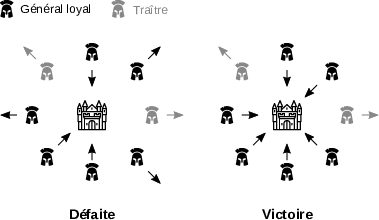
\includegraphics{chapters/img/byzantine-generals-attack.png}

}

\caption{Attack of the Byzantine generals on the city: success and
failure.}

\end{figure}%

The problem is to find a strategy (i.e., an algorithm) that ensures all
loyal generals agree on the battle plan. The traitors will then retreat,
but since their number is assumed to be limited, the attack will still
succeed.

The situation makes achieving consensus difficult. Appointing a
commander to whom subordinate generals would obey is not feasible
because the commander could be a traitor. Lamport, Shostak, and Pease
demonstrated that the problem can be solved absolutely if and only if
the loyal generals represent more than two-thirds of all
generals\footnote{This property is demonstrated in Lamport et al.'s
  original article. The more precise condition is \(n \ge 3 m + 1\),
  where \(n\) is the total number of generals and \(m\) the number of
  traitors.}; in other words, there cannot be more than one-third
traitors within the army.

The metaphor of the Byzantine generals directly applies to distributed
systems---that is, systems whose components are separated and must
communicate to synchronize. The generals represent system components,
the traitors represent faulty components, and the messages are data
transmitted between components. The goal is to obtain an algorithm that
can detect failures, known as Byzantine faults, and allow the other
components to exclude them. The resulting resilience is called Byzantine
Fault Tolerance (BFT); the system is said to be BFT-compliant.

Initially, the problem was described for computer systems relying on
components located in different places, where reliable data transmission
is critical, such as aerospace and aviation systems\footnote{The Boeing
  777's infrastructure relies notably on the ARINC 629 data bus, which
  quadruple-replicates sent messages to ensure a result with minimal
  latency. --- Elaine Ou, ``Byzantine Fault Tolerant Airplanes,''
  February 12, 2017:
  \url{https://elaineou.com/2017/02/12/byzantine-fault-tolerant-airplanes/}.}.
But it also concerns (and is of interest to us here) peer-to-peer
systems based on a horizontal network of participants, particularly
crypto-economic systems like Bitcoin, where network nodes need to agree
on the contents of a ledger. The objective is then to find an algorithm
that allows all honest nodes to reach consensus in the presence of
malicious (or ``Byzantine'') nodes.

Before Bitcoin, the problem was solved using so-called ``classical''
algorithms based on the ideas of Lamport, Shostak, and Pease. The most
well-known is probably the PBFT (Practical Byzantine Fault Tolerance)
consensus algorithm, developed by Miguel Castro and Barbara Liskov in
1999, which allowed a given number of participants to agree while
handling thousands of requests per second with latency under a
millisecond.

Long before Bitcoin, Wei Dai and Nick Szabo considered using this type
of algorithm for their electronic money systems, b-money and bit gold.
Similarly, many crypto-economic systems still employ them today for
performance reasons, such as Ethereum, whose consensus is based on the
Casper FFG algorithm.

However, these algorithms impose strong constraints: nodes must know all
other nodes and must communicate with each other. As a result, nodes
authorized to participate in the consensus must be selected before the
algorithm is launched, usually through Proof of Authority (PoA) using a
whitelist of nodes, or Proof of Stake (PoS) based on the amount of units
owned or delegated. This implies less robustness because validators are
known to everyone and are therefore more exposed to attacks.

Bitcoin addresses this problem differently, using a new type of
algorithm: Nakamoto's consensus algorithm based on proof of work. This
method is more robust in the sense that network nodes do not need to
know all other nodes, and no identification is required.

Since Bitcoin's primary role is the transfer of value, the goal is to
agree on who owns what---that is, the \emph{state} of the system.
Satoshi Nakamoto's proposed solution involves using a ledger recording
all transactions made since the system's launch: ``The only way to
confirm the absence of a transaction is to be aware of all
transactions\footnote{Satoshi Nakamoto, \emph{Bitcoin: A Peer-to-Peer
  Electronic Cash System}, October 31, 2008.}.'' This ledger, forming
the system's \emph{history}, is organized as a succession of blocks of
transactions, such that it is commonly called the \emph{blockchain}.
Network nodes each maintain a complete copy of the chain, transmitting
its elements upon request.

New blocks are added to the chain regularly through the production of a
proof of work. The actors performing this operation are called miners.
Network nodes reach consensus by considering the longest chain as the
correct one. Thus, as Satoshi Nakamoto wrote:

``The proof-of-work chain is a solution to the Byzantine Generals
Problem\footnote{Satoshi Nakamoto, ``Re: Bitcoin P2P e-cash paper,''
  November 13, 2008, 22:56:55 UTC:
  \url{https://www.metzdowd.com/pipermail/cryptography/2008-November/014849.html}.}.''

The innovative aspect of this algorithm is that it solves the problem
probabilistically rather than absolutely\footnote{More precisely, it
  sacrifices some of the security property in Lamport's sense to improve
  Byzantine fault tolerance.}. Consequently, transactions included in
the ledger are never strictly final but are considered such after a
certain time, probabilistically speaking. This functioning requires only
51\% honest validators, instead of the 67\% required by classical
algorithms.

\section*{Proof of Work}\label{la-preuve-de-travail}
\addcontentsline{toc}{section}{Proof of Work}

\markright{Proof of Work}

Proof of Work (PoW) is a process that allows a computing device to
objectively and quantifiably demonstrate that it has expended energy.
This method is used to select computers for access to a service or
privilege.

Proof of Work is a mechanism against Sybil attacks, making it difficult
for an actor to create excessive identities to take control of the
network. A Sybil attack is one where, in an open network based on a
reputation system, profiles are duplicated cheaply to disrupt
operations. This is a particularly prevalent issue on social media,
where bot accounts are mass-created to boost the visibility of specific
content.

The concept of Proof of Work was first described by Cynthia Dwork and
Moni Naor in 1992, in an article presenting a method to combat spam in
email inboxes\footnote{Cynthia Dwork, Moni Naor, ``Pricing via
  Processing or Combatting Junk Mail,'' 1992.}. The term ``proof of
work'' was introduced in 1999 by Markus Jakobsson and Ari
Juels\footnote{Markus Jakobsson, Ari Juels, ``Proofs of Work and Bread
  Pudding Protocols (Extended Abstract),'' 1999.}.

Dwork and Naor's idea was implemented by British cypherpunk Adam Back in
1997 with Hashcash, an algorithm that easily produces proofs of work
using a hash function, mainly intended for email\footnote{Adam Back,
  ``{[}ANNOUNCE{]} hash cash postage implementation,'' March 28, 1997,
  16:52:26 UTC:
  \url{https://cypherpunks.venona.com/date/1997/03/msg00774.html}; Adam
  Back, ``Hashcash --- A Denial of Service Counter-Measure,'' August 1,
  2002: \url{http://www.hashcash.org/hashcash.pdf}.}. This
implementation was later incorporated into Hal Finney's reusable
proof-of-work (RPOW) system implemented in 2004.

Hashcash's Proof-of-Work algorithm involves finding a partial collision
of the chosen hash function---that is, obtaining two messages whose
hashes start with the same data bits. Starting from version 1.0 released
in 2002, the goal is more precisely to find a partial collision for the
zero hash, meaning finding a preimage whose hash starts with a
determined number of binary zeros. Since the hash function is one-way
(preimage resistant), such a result can only be achieved by testing
possibilities one by one, which requires energy. The obtained preimage
is called a proof of work.

The proof of work is performed by successively computing hashes of a
string composed of base information and a varying number, called the
counter or nonce. The base information generally includes context
details indicating when the proof of work was produced (identifier,
date, time, protocol, etc.) to demonstrate that the proof has not been
previously used.

Let's take an example to illustrate this. First, we choose base
information specific to the context: to produce a proof of work related
to this book and its writing date, we might opt for the base information
\texttt{20231031181000:BitcoinElegance:}. Then, we determine the degree
of the proof of work---that is, the number of binary zeros the hash must
start with, here 16. Next, we search for the desired result by
incrementing the nonce: at each iteration, we concatenate it with the
base information and check if the hash of the whole satisfies the
requirement. The work stops when the hash begins with a sufficient
number of zeros; in this case, after 95,690 attempts. Our proof of work
is thus:

\begin{verbatim}
20231031181000:BitcoinElegance:95690
\end{verbatim}

And the corresponding hash, starting with 4 hexadecimal zeros (i.e., 16
binary zeros), is:

\begin{verbatim}
0000387b99b1412e3cb6e49548cc0d11bdc797138e1a0f5ff095279a710b895a
\end{verbatim}

The steps of this procedure are detailed in
Table~\hyperref[table:hashcash-hashes]{8.1}.

\phantomsection\label{table:hashcash-hashes}
\begin{longtable}[]{@{}rc@{}}
\caption{Searching for the proof of work using the base information
\texttt{20231031181000:BitcoinElegance:}.}\tabularnewline
\toprule\noalign{}
\textbf{Nonce} & \textbf{Hash (SHA-256)} \\
\midrule\noalign{}
\endfirsthead
\toprule\noalign{}
\textbf{Nonce} & \textbf{Hash (SHA-256)} \\
\midrule\noalign{}
\endhead
\bottomrule\noalign{}
\endlastfoot
0 & 933c448c18e334c1cc5191f035d8581af611417578392b2d695d521c29b396d5 \\
1 & 50530c98d1b171826b3d26fa5442e4ce7aa1f8a1277b71bc74d3adc1cd88b9ae \\
2 & fa27ed560df22d676d69966c9a981c5adfc395b4e7f78ca54d2593a98fd2ea38 \\
3 & 011692df53a84ecdddcd154de4f329e7311090580adb189e8360ea1729d75c99 \\
95,690 &
0000387b99b1412e3cb6e49548cc0d11bdc797138e1a0f5ff095279a710b895a \\
\end{longtable}

Statistically, this type of search requires trying 65,536 possibilities
(\(2^{16}\)) to find a solution. On average, producing such a proof of
work demonstrates that a commensurate effort has been made. Moreover,
there is an asymmetry between production and verification, the latter
requiring only a single application of the hash function and thus being
low-cost.

The average production cost imparts a certain scarcity to proofs of
work: the higher their degree, the harder they are to produce. This is
why they can be used as quality markers for email, as in Hashcash, or as
basic monetary units, as in bit gold and RPOW.

Bitcoin's mining incorporates Hashcash's proof-of-work process in a
variant form: the goal is to find a hash less than a specific target
value, rather than a hash starting with a determined number of zeros.
This process is applied between blocks of transactions, so these
blocks---or rather their headers, as we will explain below---constitute
the proofs of work themselves.

In Bitcoin, the role of proof of work is twofold: to require a cost for
creating new bitcoins and to ensure the network can reach consensus. On
one hand, it aims to impose a cost on the unit of account. This echoes
models that preceded Bitcoin, and it's why Hal Finney went so far as to
describe bitcoins as ``POW tokens'' in 2009\footnote{Hal Finney,
  ``Bitcoin v0.1 released,'' January 24, 2009, 16:48:03 UTC:
  \url{https://www.metzdowd.com/pipermail/cryptography/2009-January/015036.html}.}.
However, bitcoins are not exactly proofs of work in the sense that their
production difficulty is variable, evolving according to the total
computing power deployed on the network. Except in the edge case of the
protocol's minimum difficulty, the goal is to ensure that unit
production requires energy, not to demand a fixed work cost. On the
other hand, proof of work aims to guarantee network consensus by
ensuring that honest nodes agree on who owns what. It limits access to
block production: the selection of the validator (miner) is based on the
amount of energy expended. Here, proof of work serves its role as a
defense against Sybil attacks by preventing attackers from setting up a
large number of nodes to control the system\footnote{``If the majority
  were based on one-IP-address-one-vote, it could be subverted by anyone
  able to allocate many IPs. Proof-of-work is essentially
  one-CPU-one-vote.'' --- Satoshi Nakamoto, \emph{Bitcoin: A
  Peer-to-Peer Electronic Cash System}, October 31, 2008.}.

This functioning means that the blockchain forms a chain of proofs of
work, summarizing all the work done since inception. Thus, the chain
creates a linear history that is difficult to alter, as we will see.

\section*{The Blockchain}\label{la-chauxeene-de-blocs}
\addcontentsline{toc}{section}{The Blockchain}

\markright{The Blockchain}

The blockchain is, as its name suggests, a data structure that groups
all transactions made since the system's launch. This structure is a
series of timestamped and worked blocks of transactions. It begins with
a genesis block, valid by default, from which blocks are counted: this
index is called the \emph{height} and indicates the block's position in
the chain in mining order. Blocks can also be counted in the other
direction from the most recently mined block, in which case we speak of
\emph{depth}.

Each block has a unique identifier that distinguishes it from others.
This is obtained by hashing the block's header (the data placed before
the transactions) using double SHA-256. Each block contains the
identifier of the previous block, so the blocks are linked to form a
chain. Since only the header is involved in calculating the identifier,
the blockchain can actually be reduced to a chain of headers, to which
transactions are cryptographically linked. The identifier starts with a
certain number of zeros, indicating that work has been required. Thus,
the block itself constitutes the proof of work.

All blocks are organized the same way, so by examining one in detail, we
can understand how the chain is structured. Let's study a block from
Bitcoin's main version (BTC), taking as an example block height 751,005,
mined on August 25, 2022, which contains six transactions.

Each block breaks down into an 80-byte header containing its essential
information and a raw sequence of transactions. By convention, the first
transaction in the block is the coinbase transaction used to reward the
miner for this block, as we will see later.

The header is divided into six elements: the block version, the previous
block's identifier linking it to the current block, a Merkle root that
cryptographically binds all transactions to the header, the block's
timestamp, the network's target value, and the nonce related to mining.
The different pieces of information in the header are transmitted with a
reversed byte order (called ``little-endian'') compared to the standard
reading order (``big-endian''). We present them here in the standard
order.

\subsection{Block Version}\label{block-version}

The block version indicates the set of rules the block adheres to.
Historically, version 1 signified compliance with the rules originally
defined by Satoshi. Versions 2 to 4 were used to enforce protocol
changes between 2013 and 2015. Since 2016, this version field is used
for miners to signal in the context of a soft fork implementation via
BIP-9 or an equivalent mechanism. The version field of our block is:

\begin{verbatim}
0b00100000000000000000000000000100
\end{verbatim}

\subsection{Previous Block Identifier}\label{previous-block-identifier}

The previous block identifier links the current block's header to the
previous block's header. In the case of the genesis block, this field is
conventionally set to zero. In our block, it is the identifier of block
751,004, which is:

\begin{verbatim}
000000000000000000073ad6c18c81f2f67b2ca5b5ace8d23cce95812af8c7b6
\end{verbatim}

\subsection{Merkle Root}\label{merkle-root}

The third element of the header is the Merkle root, corresponding to the
final hash of the transaction arrangement in a Merkle tree.

A Merkle tree, also known as a hash tree, is a data structure
conceptualized in 1979 by cryptographer Ralph Merkle to verify the
contents of a data volume without inspecting all of it. In such a
structure, data (forming the leaves of the tree) are arranged in a
certain order and hashed individually:

\[H_A = \mathrm{SHA256d}(~\mathrm{tx}_A~)\]

Then, the resulting hashes are concatenated in pairs (the second hash
placed after the first) and the combined hash is computed:

\[H_{A\!B} = \mathrm{SHA256d}(~H_A \parallel H_B~)\]

This process is repeated. If the number of hashes to combine is odd, the
last hash is concatenated with itself:

\[H_{E\!F\!E\!F} = \mathrm{SHA256d}(~H_{E\!F} \parallel H_{E\!F}~)\]

Once only one hash remains, the tree is complete: the final hash
obtained is the Merkle root.

The Merkle root of block 751,005 is:

\begin{verbatim}
268a15b56fe847a067624bd0be186c375baccae9ac6db304438e9da657fe51d9
\end{verbatim}

Including the Merkle root in the header prevents anyone from modifying,
adding, or deleting a transaction without altering the header itself and
reproducing the proof of work. Thus, all transactions are attached to
the header, ensuring the block's integrity.

\begin{figure}

{\centering 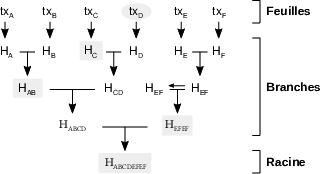
\includegraphics{chapters/img/merkle-tree.png}

}

\caption{Representation of a Merkle tree with six leaves.}

\end{figure}%

This organization is particularly useful for lightweight wallets (known
as Simplified Payment Verification or SPV wallets) that do not store the
entire blockchain but only the chain of headers, which is much less
voluminous (just over 62 MB as of November 2023). Indeed, to verify the
presence of a transaction in a block, they can simply request the
related branch information (Merkle path) and perform the hashes
themselves\footnote{Demonstrating that a leaf is part of a Merkle tree
  requires computing a number of hashes proportional to the binary
  logarithm of the number of leaves (\(\log_{2}(n)\)), not proportional
  to the number of leaves \(n\). For a block with 3,000 transactions (a
  high average on BTC), this represents 12 hashes of 32 bytes to obtain
  and 12 hashes to compute.}. For example, a user wanting to confirm the
transaction \(\mathrm{tx}_D\) needs only to request \(H_C\),
\(H_{A\!B}\), and \(H_{E\!F\!E\!F}\) from network nodes and perform the
necessary hashes to compare the obtained root with that in the header.
This greatly reduces the load on lightweight wallets.

Since the activation of SegWit on August 24, 2017, each block contains
an additional Merkle tree, subordinate to the classical transaction tree
described above. This is the witness tree, which is the tree of
transactions including SegWit transaction signatures (separated from
classical transactions). The root of the witness tree is placed in the
coinbase transaction, so it is included in the main Merkle root,
ensuring the integrity of the whole.

\subsection{Timestamp}\label{timestamp}

The timestamp indicates the date and time of the block's construction as
declared by the miner. Technically, it is given by the Unix time, which
is the number of seconds elapsed since January 1, 1970, at 00:00:00 UTC.
For our block, the timestamp is \(1661407005\), corresponding to August
25, 2022, at 5:56:45 AM (UTC).

The miner cannot choose this timestamp arbitrarily. The declared time
must be in the future relative to the Median Time Past (MTP)---the
median of timestamps of the last 11 blocks, which generally lags about
an hour behind real time---and must not exceed the receiver nodes'
clocks by more than two hours. This relatively permissive constraint
allows the network time to remain reasonably consistent with reality.

\subsection{Target Value}\label{target-value}

The target value is the maximum value that the block identifier can take
for the block to constitute a valid proof of work. The smaller this
target value, the harder it is to find a solution and mine a block. It
is determined by the network according to the difficulty adjustment
algorithm rules.

The target value is encoded as a floating-point number where the first
byte represents a specific exponent and the next three bytes determine
the mantissa. Here, it equals
\(\mathtt{0x09ed88} \times 256^{(\mathtt{0x17} - 3)}\), which is:

\begin{verbatim}
00000000000000000009ed880000000000000000000000000000000000000000
\end{verbatim}

This information also provides the block's mining difficulty, which is
inversely proportional to the target value. It is the quotient of the
system's maximum target value by the network's target value\footnote{Denoting
  \(c\) as the target value, the difficulty is defined by:
  \[d = \frac{C_{\mathrm{max}}}{c}\] where
  \(C_{\mathrm{max}} = \mathtt{0x00ffff} \times 256^{26}\) is the
  network's maximum target value.}. The protocol's minimum difficulty is
therefore 1, and that of our block (rounded to the nearest whole number)
is \(28,351,606,743,494\), representing a massive differential! It also
gives the block's amount of work, which is the average number of hashes
needed to find a solution\footnote{Mathematically, the work of a block
  is the quotient of the number of possible hashes by the number of
  hashes satisfying the problem. Denoting \(c\) as the target value, the
  work is: \[T = \frac{2^{256}}{c + 1} ~.\]}.

\subsection{Nonce}\label{nonce}

The nonce denotes the number that the miner varies to produce the proof
of work. The word comes from the English expression ``for the nonce,''
meaning ``for the occasion,'' indicating its specific role\footnote{A
  popular etymology claims it's a contraction of ``number used once,''
  but this is incorrect.}. The miner also varies an additional nonce
within the coinbase transaction, as the nonce field is too small (8
bytes) for the current mining difficulty. The nonce of our block is
\(4,224,551,499\).

These last two parameters (target value and nonce) relate to the proof
of work and are involved in formulating the mathematical problem solved
by the miner. This problem presents as a mathematical inequality.
Denoting \(c\) as the network's target value and \(\mathrm{HB}\) as the
block header, the task is to find a nonce \(n\) such that:

\[\mathrm{SHA256d} ( \ \mathrm{HB} ( \ n \ ) \ ) ~ \le ~ c\]

As mentioned, the result is used as the block's identifier. The proof of
work is easily verifiable: each network member can, based on the block's
data, ensure the miner has found a valid solution. In our case,
comparing the identifier and the target value, we indeed obtain a result
satisfying the required inequality:

\[\begin{aligned}
\mathtt{0x000000000000000000065aebf106c8824f4b565d54d6d6df32498b2b041cfd07} & \le \\ \mathtt{0x00000000000000000009ed880000000000000000000000000000000000000000} & ~
\end{aligned}\]

\begin{figure}

{\centering 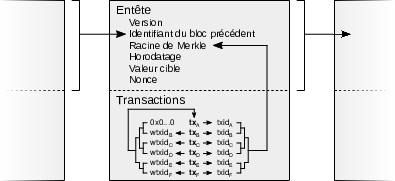
\includegraphics{chapters/img/bitcoin-segwit-block.png}

}

\caption{Diagram of a Bitcoin block (with SegWit).}

\end{figure}%

\section*{Mining Revenue}\label{le-revenu-du-minage}
\addcontentsline{toc}{section}{Mining Revenue}

\markright{Mining Revenue}

One of Bitcoin's innovations is rewarding transaction confirmations
using its internal unit of account. This feature creates an economic
incentive encouraging miners to behave properly, contributing to the
system's robustness.

The reward for adding a block to the chain partly comes from the
protocol's monetary creation, hence the term ``mining'' used to describe
this activity. The process is analogous to real-world gold extraction:
miners deploy capital and expend energy to obtain new bitcoins. As
Satoshi noted in the whitepaper:

``The steady addition of a constant amount of new coins is analogous to
gold miners expending resources to add gold to circulation\footnote{Satoshi
  Nakamoto, \emph{Bitcoin: A Peer-to-Peer Electronic Cash System},
  October 31, 2008.}.''

The second part of the reward comes from transaction fees paid by users,
collected from the transactions included in the block. The total is
forwarded to the miner when the block is verified and accepted by the
network.

Mining is thus the economic activity of gathering transactions into a
block, producing the proof of work, and broadcasting the result across
the network. Here, we distinguish it from simple hashing, which involves
only performing calculations to create the proof of work and can be done
independently of transaction selection, particularly within mining
pools. In this context, miners are individuals or groups performing the
complete activity, and entities merely setting up machines and
delegating their power over transaction selection are merely
``hashers.''

Mining operates cyclically. First, the miner selects transactions from
their node's transaction pool (called the \emph{mempool}). Then, they
construct a candidate block by setting a header, assembling the
transactions, and carefully creating a coinbase transaction that rewards
them. They then vary the nonce and other elements of the candidate block
to produce the proof of work. If they find a solution, they broadcast
the block to the network as quickly as possible so other nodes can
verify it and accept it as the new block in the chain. If not, and a new
block is found in the meantime, the miner accepts it and abandons their
candidate block. In either case, the process restarts with different
transactions.

The mining reward is thus collected by the miner by including a coinbase
transaction within the block. This must, by convention, be the first
transaction of the block. It has a unique input that does not reference
any existing transaction. The coinbase transaction is also called the
base of the coin because it is from this that new bitcoins are formed.
The miner directs this transaction to an address they control, so they
are rewarded only if their block is valid in the eyes of the network.
The reward the miner can allocate to themselves must be less than or
equal to the sum of the monetary creation and transaction fees. Thus,
the miner can choose to reward themselves less than what the protocol
allows, although this lacks direct economic sense\footnote{In December
  2017, the miner of block 501,726 rewarded themselves with the tidy sum
  of 0 BTC!}.

Monetary creation occurs entirely through the coinbase transaction. All
bitcoins in the system result from a series of transfers starting with
such a transaction.

The particularity of this monetary creation is that it's fixed over time
and isn't proportional to the computing power deployed. This is made
possible by the difficulty adjustment algorithm, which derives from the
fact that the system acts as a distributed timestamp server. Indeed,
since blocks are timestamped, it's possible to measure their past
production rate and adjust mining difficulty accordingly. As Satoshi
wrote:

``To compensate for increasing hardware speed and varying interest in
running nodes over time, the proof-of-work difficulty is determined by a
moving average targeting an average number of blocks per hour. If
they're generated too fast, the difficulty increases\footnote{Satoshi
  Nakamoto, \emph{Bitcoin: A Peer-to-Peer Electronic Cash System},
  October 31, 2008.}.''

In Bitcoin's main version, the targeted interval between each block
(block time) is 10 minutes, or 600 seconds. The adjustment occurs every
2,016 blocks, roughly every two weeks, based on the simple average block
time over that period. The new target value is calculated\footnote{In
  Bitcoin Core, the difficulty adjustment algorithm is described by the
  \texttt{CalculateNextWorkRequired} function in the file
  \texttt{pow.cpp}. The variation is limited to a factor of 4 (both
  multiplication and division) to prevent instabilities. The algorithm
  \emph{overestimates} the deployed computing power because the elapsed
  time is measured over 2,015 intervals, not 2,016 as it should be.}
from the previous target value (\(c_{k-1}\)) and the elapsed time since
the last adjustment (\(t_{k-1}\)):

\[c_{k} = \frac{c_{k-1} \cdot t_{k-1}}{2016 \cdot 600}\]

Thanks to this adjustment, bitcoin has a determined monetary policy, not
subject to the direct arbitrariness of a trusted third party or the
amount of deployed capital. This characteristic differentiates it from
fiat money (like the dollar), which is issued discretionarily by a
central bank, or precious metals (like gold), whose extracted quantity
varies and follows market demand in the long term. This monetary policy
was precisely described for the first time by Satoshi Nakamoto in his
launch email on January 8, 2009, where he wrote:

``The total amount of coins in circulation will be 21,000,000. They will
be distributed to network nodes when they create blocks, with the amount
issued halving every 4 years.

First 4 years: 10,500,000 coins\\
Next 4 years: 5,250,000 coins\\
Next 4 years: 2,625,000 coins\\
Next 4 years: 1,312,500 coins\\
etc\ldots{}

Once this sum is exhausted, the system can support transaction fees if
necessary. It relies on open market competition, and there will probably
always be nodes willing to process transactions for free\footnote{Satoshi
  Nakamoto, ``Bitcoin v0.1 released,'' January 8, 2009, 19:27:40 UTC:
  \url{https://www.metzdowd.com/pipermail/cryptography/2009-January/014994.html}.}.''

This policy is, of course, coded into the system, where it is called a
subsidy.

The main originality of this monetary policy is that monetary creation
is abruptly halved every 210,000 blocks (approximately every four years)
during what is commonly called a \emph{halving}. By 2023, three halvings
had already occurred on the main Bitcoin network: the first on November
28, 2012, when the protocol's subsidy dropped from 50 bitcoins per block
to 25; the second on July 9, 2016, reducing it to 12.5 bitcoins per
block; and the third on May 11, 2020, further reducing it to 6.25
bitcoins per block. The next halving is expected around April 2024,
after which new bitcoins issued will be 3.125 per block. Unless the
consensus rules change, the 33rd and final halving will occur around
2140, as the monetary creation per block will then fall below one
satoshi, effectively zero when truncated to whole units.

In the long term, this atypical monetary policy makes bitcoin a
fixed-quantity currency. Indeed, the maximum amount of bitcoins in
circulation is expected to approach a limit over time: the famous 21
million cap. This is simply a deduction from the aforementioned issuance
conditions, expressed mathematically by the convergence of the sums of
amounts mined between halvings\footnote{This convergence is illustrated
  by Zeno's paradox of Achilles and the tortoise. The series
  \(\left( \sum_{i=1}^{n} (1/2)^i \right)\) converges to \(1\) as
  \(n\to+\infty\).}:

\[N_{\mathrm{max}} = \sum_{i=0}^{+\infty} \left( {210,000 \cdot \frac{50}{2^i}} \right) = 21,000,000 \cdot \sum_{i=1}^{+\infty} \left(\frac{1}{2}\right)^i = 21,000,000\]

The 21 million limit is an upper bound: in the absence of a change in
the consensus rules, it will never be formally reached due to the
optional nature of the mining reward, the discrete nature of the units,
and the irreversible loss of bitcoins. Additionally, bitcoins whose
owners have lost their private keys significantly reduce the actual
quantity of bitcoins in circulation, though this isn't accounted for in
the calculation.

Monetary creation is thus intended to diminish and become negligible,
and this will happen sooner than one might think. Indeed, by 2023, the
number of spendable bitcoins had already exceeded 19.5 million.
Therefore, logically, this subsidy should be replaced by the other
source of miner revenue: transaction fees\footnote{``Once a
  predetermined number of coins have entered circulation, the incentive
  can transition entirely to transaction fees and be inflation-free.''
  --- Satoshi Nakamoto, \emph{Bitcoin: A Peer-to-Peer Electronic Cash
  System}, March 24, 2009.}.

Transaction fees are commissions paid by users for confirming their
transactions. Transaction fees can be paid directly by the sender
(client) or indirectly by the recipient (merchant) through a discount on
the sold product. They are collected by the miner on each transaction in
the block according to an implicit rule: it is the difference between
the transaction's input amount and its output amount. This difference
can be zero (free transaction), but it is always accounted for. Fees are
added to the coinbase transaction indistinctly from bitcoins generated
by monetary creation. Bitcoin thus incorporates an internal and
optimized transaction fee system, avoiding unnecessary bloating of
transactions and blocks.

The existence of transaction fees is intended to persist by design, even
if they become very low. Contrary to Satoshi's opinion, confirming a
transaction generally has a cost, even marginal\footnote{The only
  conceivable case of a free transaction is a large consolidation
  transaction that would reduce miners' load by significantly decreasing
  the set of unspent transaction outputs.}, and a transaction that pays
too few fees relative to the load it brings has no economic reason to be
confirmed. Therefore, there's no reason to imagine the blockchain
stopping.

Moreover, protocol rules usually restrict block space through an
explicit limit on block size (or weight). This restriction creates a
production ceiling that, when reached, causes a rational miner to select
transactions paying the highest fee rates, all else being equal. Thus,
in the case of network congestion, there's an auction effect that can
drastically increase the average fee level.

Although fees are the main way envisioned to compensate miners in the
long run, alternative financing methods have been proposed.

The first is tail emission, which involves maintaining a constant
monetary creation over time to ensure mining revenue doesn't drop too
low\footnote{Peter Todd, ``Surprisingly, Tail Emission Is Not
  Inflationary,'' July 9, 2022:
  \url{https://petertodd.org/2022/surprisingly-tail-emission-is-not-inflationary}.}.
Introducing this feature would alter bitcoin's monetary policy and
eliminate the 21 million cap, making it highly controversial.

For example, tail emission has been implemented in the Monero variant
since 2015. It became effective on June 9, 2022, after which 0.3 monero
are created per minute, representing an annualized monetary creation
rate of 0.87\% at that time. A similar tail emission exists in Dogecoin
since 2015, at 10,000 dogecoins per minute, with an annualized rate of
3.7\% as of November 2023.

The second proposed financing method is demurrage, or holding cost,
which involves taxing currency that has remained idle for a given
time\footnote{Jorge Timón, ``Freicoin: bitcoin with demurrage,''
  February 24, 2011, 11:56:03 UTC:
  \url{https://bitcointalk.org/index.php?topic=3816.msg54170\#msg54170}.}.
Satoshi's bitcoins, representing a significant financial windfall, are
particularly affected. However, this would infringe upon Bitcoin's
property system, making it unlikely for this method to gain traction.

\section*{The Longest Chain}\label{la-chauxeene-la-plus-longue}
\addcontentsline{toc}{section}{The Longest Chain}

\markright{The Longest Chain}

Now let's address the central topic of this chapter: achieving consensus
through mining. As we have explained, mining is the process allowing
miners to add blocks to the chain, for which they are rewarded. But we
have not detailed how this enables reaching agreement in an antagonistic
context, with malicious ``Byzantine'' actors present.

Nodes follow a protocol composed of network rules, allowing them to
communicate, and consensus rules, concerning the form of transactions
and blocks, which we will detail in
Chapter~\hyperref[ch:changement]{10}. Nodes that violate these rules
have their connections closed by their peers and are blacklisted if
necessary. It is therefore impossible to have a transaction or block
accepted by the network that is not valid according to the consensus
rules.

Nonetheless, Byzantine nodes can sow discord while respecting the
consensus rules by producing competing blocks. Indeed, nothing
inherently prevents an attacker from producing valid transaction blocks
not attached to the main branch and submitting them to the network.

This problem is solved through a simple yet effective principle: the
longest chain principle. This was described by Satoshi in the
whitepaper:

``The majority decision is represented by the longest chain, which has
the greatest proof-of-work effort invested in it\footnote{Satoshi
  Nakamoto, \emph{Bitcoin: A Peer-to-Peer Electronic Cash System},
  October 31, 2008.}.''

Network nodes agree by selecting the chain with the most accumulated
work, which generally materializes as the chain with the most
blocks\footnote{In reality, initially, it was indeed the chain with the
  most blocks that was selected. But this principle was redefined on
  July 25, 2010, in version 0.3.3 of the software to account for work.}.
When a chain with strictly more work is published, nodes follow that
chain, whether it continues from the last one or references an older
branch. This rule ensures nodes always follow the chain where a greater
amount of energy has been invested. The consensus algorithm resulting
from applying this principle is called Nakamoto's Proof-of-Work
consensus algorithm, in honor of its creator.

The best way to understand this algorithm's functioning is to consider a
fork in the chain. Such a fork can be created by a malicious actor but
is usually generated accidentally when two distant miners each find a
different block within a short time interval, and network nodes receive
different blocks first. There's then no way to differentiate between the
two branches, as both are correct under the longest chain principle.
This type of accidental fork is common and occurs occasionally on the
network due to latency.

This situation and its resolution were described by Satoshi in the
whitepaper:

``If two nodes broadcast different versions of the next block
simultaneously, some nodes may receive one or the other first. In that
case, they work on the first one they received but save the other branch
in case it becomes longer. The tie is broken when the next proof-of-work
is found, and one branch becomes longer; the nodes that were working on
the other branch then switch to the longer one\footnote{Satoshi
  Nakamoto, \emph{Bitcoin: A Peer-to-Peer Electronic Cash System},
  October 31, 2008.}.''

The network goes through three stages. Initially, it behaves as
expected: miners extend the longest chain, on which the rest of the
nodes coordinate. Then, the conflict occurs: two correct branches
coexist, and miners work to extend the chain from the block they
received first. Finally, the fork is resolved: a miner finds a new
block, and their chain, now longer, is accepted by the network.

A reorganization then occurs, reconciling the network nodes. The block
from the weaker branch is considered incorrect and set aside. We say
this block is orphaned as it loses its attachment to the parent
chain\footnote{The somewhat ambiguous term ``orphan block'' was
  introduced by Satoshi Nakamoto in the first version of the software.
  It is also called an ``uncle block'' (referring to its lack of
  productive descendants) or a ``stale block.''}. The stronger branch
(with the most accumulated work) is considered the correct version of
the chain.

\begin{figure}

{\centering 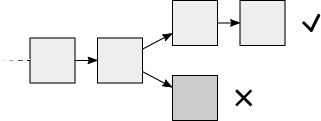
\includegraphics{chapters/img/blockchain-common-fork.png}

}

\caption{Diagram of a common chain fork.}

\end{figure}%

All conflicts on the network are resolved this way, which imparts
particular characteristics to Nakamoto's algorithm and, by extension, to
Bitcoin.

First, this functioning imposes two major security constraints. The
first is that the network's mining security relies on the assumption
that a majority of the computing power (``51\%'') behaves honestly. As
Satoshi explained:

``The system is secure as long as honest nodes collectively control more
CPU power than any cooperating group of attacker nodes\footnote{Satoshi
  Nakamoto, \emph{Bitcoin: A Peer-to-Peer Electronic Cash System},
  October 31, 2008.}.''

The second is that the security of a given transaction is probabilistic
and depends on its depth in the chain. The transaction is first verified
by the network (zero confirmation), then confirmed within a block (one
confirmation), and eventually considered irreversible, generally after
six confirmations for ordinary amounts on Bitcoin's main version. This
constrains the user to estimate the number of confirmations they must
wait for based on the desired security.

This particularity is reflected in mining through the coinbase maturity,
which is the number of confirmations required before the coinbase
transaction's output becomes spendable. This constraint is implemented
to prevent misuse of funds due to a shallow reorganization. The delay on
the BTC network is currently 101 confirmations.

Nakamoto's algorithm also has three main advantages. First, it has the
benefit of an objective criterion to rely on: everyone can reconstruct
the chain from the genesis block and confirm it is the correct chain.
Even in the extreme case of a global and prolonged network partition due
to war or natural disaster, the system can eventually
recoordinate\footnote{Satoshi Nakamoto, ``Re: Anonymity,'' July 8, 2010,
  19:12:00 UTC:
  \url{https://bitcointalk.org/index.php?topic=241.msg2071\#msg2071}.}.

Second, it allows open participation in consensus: all that is required
of a miner is a valid proof of work, making mining anonymous by essence.

Finally, this proof-of-work algorithm ensures network robustness: a
miner doesn't need to know all other participants, allowing the network
to be composed of tens (or even hundreds) of thousands of nodes.

\section*{Resistance to Double
Spending}\label{la-ruxe9sistance-uxe0-la-double-duxe9pense}
\addcontentsline{toc}{section}{Resistance to Double Spending}

\markright{Resistance to Double Spending}

Double spending refers to an actor successfully having two transactions
accepted by the network in succession, intending to destabilize the
system's state and benefit from it in some way. The second transaction
may cancel the first, wherein the malicious actor makes a transfer back
to themselves.

Double spending poses a problem for unconfirmed transactions---that is,
transactions that have been broadcast to the network, verified by nodes,
and placed in their mempools but not yet included in a block in the
chain. No consensus has been reached about these transactions, but a
merchant may choose to accept them when the amounts involved are
small\footnote{In a forum message in July 2010, Satoshi wrote about
  accepting unconfirmed transactions: ``I think it will be possible for
  a payment processing company to provide a service of rapid transaction
  distribution with sufficient verification in 10 seconds or less.
  Network nodes accept only the first version of a transaction they
  receive to include in the block they're working to generate. When
  broadcasting a transaction and someone else broadcasts a double-spend
  at the same time, it's a race to propagate to as many nodes as
  possible. If one has a slight lead, it spreads geometrically faster on
  the network and reaches most nodes. {[}\ldots{]} The payment processor
  has connections to many nodes. When it receives a transaction, it
  sends it out and at the same time monitors the network for
  double-spends. If it receives a double-spend on any of its many
  listening nodes, it reports the transaction as bad.'' --- Satoshi
  Nakamoto, ``Re: Bitcoin snack machine (fast transaction problem),''
  July 17, 2010, 22:29:13 UTC:
  \url{https://bitcointalk.org/index.php?topic=423.msg3819\#msg3819}.}.
The risk is that a fraudster walks away with the goods and manages to
have an alternative version of the transaction accepted by the network,
either by broadcasting it simultaneously and hoping it reaches the miner
first, by paying higher fees (which can be systematically done with
Replace-by-Fee) to bribe the miner, or by pre-mining a block containing
the transaction (Finney attack\footnote{Hal Finney, ``Re: Best practice
  for fast transaction acceptance - how high is the risk?,'' February
  13, 2011, 21:48:44 UTC:
  \url{https://bitcointalk.org/index.php?topic=3441.msg48384\#msg48384}.}).

The solution to this problem is to agree on the correct transaction to
eliminate the double spending---which is precisely the purpose of
mining. However, mining does not prevent double spending absolutely; it
is rather a resistance mechanism. Let's examine what guarantees this
characteristic.

A number of opportunistic disruptions can occur in mining activity, such
as the vector76 attack\footnote{vector76, ``Re: Fake Bitcoins?,'' August
  17, 2011, 17:37:56 UTC:
  \url{https://bitcointalk.org/index.php?topic=36788.msg463391\#msg463391}.}
or selfish mining\footnote{Ittay Eyal, Emin Gün Sirer, ``Majority is not
  Enough: Bitcoin Mining is Vulnerable,'' 2013.}, but the most
significant is the double-spending attack through chain reorganization.
This involves using a significant portion of the network's computing
power (usually a majority) to rewrite the chain's past and modify one or
more transactions. This attack was precisely described by Satoshi
Nakamoto in the whitepaper\footnote{``We consider the scenario of an
  attacker trying to generate an alternate chain faster than the honest
  chain. Even if successful, it does not open up arbitrary modifications
  {[}\ldots{]} An attacker can only try to modify one of his own
  transactions to recover the money he recently spent.'' --- Satoshi
  Nakamoto, \emph{Bitcoin: A Peer-to-Peer Electronic Cash System},
  October 31, 2008.} and in his email response to John Levine on
November 3, 2008\footnote{``Even if a malicious individual managed to
  control the network, it's not like he's instantly rich. All he could
  do is get back money he himself spent, like bouncing a check. To
  exploit this, he'd have to buy something from a merchant, wait for it
  to be shipped, then take over the network and try to get his money
  back. I don't think he could make as much money trying to pull a stunt
  like that as he could by generating bitcoins. With such a large
  botnet, he could generate more bitcoins than everyone else combined.''
  --- Satoshi Nakamoto, ``Re: Bitcoin P2P e-cash paper,'' November 3,
  2008, 16:23:49:
  \url{https://www.metzdowd.com/pipermail/cryptography/2008-November/014818.html}.}.

This attack is carried out in three steps. It can be executed using a
minority of computing power, in which case it only has a certain
probability of success. However, for simplicity, we'll assume a miner
has gathered the majority of the network's computing power. The attack
thus constitutes a 51\% attack, also known as a majority attack.

The first step is purchasing a good or service from a merchant. The
attacker conducts a legitimate bitcoin transaction in exchange for which
the merchant provides something of equivalent value---typically another
cryptocurrency or dollars from an exchange platform.

The second step involves mining a parallel chain. Once the legitimate
transaction has been confirmed within a block, the attacker constructs a
parallel chain in secret from the previous block, carefully not
revealing it to the rest of the network. Simultaneously, they create and
sign another transaction (the ``fraudulent'' one) spending the same
bitcoins as the first but sending them to an address they control. They
include this fraudulent transaction in their parallel chain. Since the
attacker controls the majority of the network's computing power, they
are sure that, at some point, this chain will be longer than the other.

The third step is the chain reorganization, depicted in
Figure~\hyperref[fig:doublespending-attack]{8.5}. The attacker continues
to mine their parallel chain until the good or service purchased is
delivered. At that point, they reveal their chain to the rest of the
network, which must accept it under the longest chain principle. Nodes
then reorganize: blocks from the old chain are discarded (orphaned),
their transactions returned to the mempool, and the new blocks are
verified and added to the chain. Since the legitimate transaction spends
the same funds as the fraudulent transaction included in the new chain,
this legitimate transaction is invalidated as a double spend. The
merchant no longer owns the bitcoins, which revert to the attacker.

\begin{figure}

{\centering 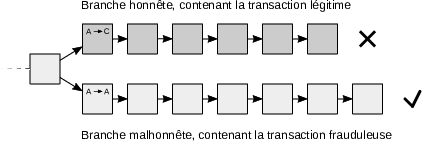
\includegraphics{chapters/img/mining-attack-doublespending.png}

}

\caption{Double-spending attack through chain reorganization.}

\end{figure}%

This is an opportunistic attack: it is motivated by gain---namely, the
acquired good or service---which must exceed the cost (material,
logistical, electrical, and software) necessary to carry it out. On the
main Bitcoin network, this cost amounts to billions of dollars
today\footnote{Braiins, ``How Much Would it Cost to 51\% Attack
  Bitcoin?,'' January 11, 2021:
  \url{https://braiins.com/blog/how-much-would-it-cost-to-51-attack-bitcoin}.}.

This attack must be distinguished from censorship, which we will
describe in Chapter~\hyperref[ch:censure]{9} and involves refusing to
confirm transactions based on arbitrary criteria. The latter relies on
incentives \emph{external} to Bitcoin's economy, as a rational miner has
no economic reason within the system not to include transactions paying
a sufficient fee rate in their blocks.

As Satoshi emphasized, the system is secure as long as the majority of
computing power is associated with honest nodes---that is, nodes not
seeking to double-spend or censor. Mining security thus relies on a
security barrier representing the financial burden on the attacker to
execute a double-spend.

This barrier is not constructed benevolently but rests on the protocol's
reward, making mining an essentially \emph{economic} process.
Specifically, resistance to double spending---that is, the difficulty of
executing a double-spend attack---directly derives from the total mining
revenue, which incentivizes nodes to remain honest. As Satoshi wrote in
the whitepaper:

``The incentive may help encourage nodes to stay honest. If a greedy
attacker is able to assemble more CPU power than all the honest nodes,
he would have to choose between using it to defraud people by stealing
back his payments or using it to generate new coins. He ought to find
it's more profitable to play by the rules, such rules that favor him
with more new coins than everyone else combined, than to undermine the
system and the validity of his own wealth\footnote{Satoshi Nakamoto,
  \emph{Bitcoin: A Peer-to-Peer Electronic Cash System}, October 31,
  2008.}.''

Not only might the reward exceed the gain from a double-spend attack,
but the value of the bitcoins used in the transaction could also
decrease due to the attack itself. Indeed, if the attack were
successful, various actors might lose confidence in the system, stop
using it for commerce, and sell some of their savings, causing the
bitcoin's exchange value and mining revenue to drop. Moreover, the
specialization of mining hardware (when it exists) increases the
attack's cost, as such hardware loses utility value. From a purely
opportunistic standpoint, it is thus usually more profitable to use
one's capital honestly.

It has happened that mining aggregates have accumulated more than 51\%
of computing power---like the GHash.io pool in July 2014---without any
attack occurring. Even if such an attack took place, it wouldn't
necessarily be fatal for the system in the long term. As Satoshi wrote:

``Even in the event of an attack, it does not enable arbitrary changes,
such as creating value out of thin air or taking money that never
belonged to the attacker. Nodes will not accept an invalid transaction
as payment, and honest nodes will never accept a block containing
them\footnote{Satoshi Nakamoto, \emph{Bitcoin: A Peer-to-Peer Electronic
  Cash System}, October 31, 2008.}.''

Thus, numerous such attacks have occurred on some Bitcoin variants over
the years, reducing their reputations in the process, but without
annihilating them. Notably, Ethereum Classic experienced several
aggressive reorganizations between 2019 and 2020.

\section*{The Mining Industry}\label{lindustrie-miniuxe8re}
\addcontentsline{toc}{section}{The Mining Industry}

\markright{The Mining Industry}

Mining is an economic activity in its own right, with the mining reward
compensating miners for the service they provide. This reward pays for
electricity costs, hardware and logistical infrastructure, and software
maintenance. It compensates for the risk of producing orphaned blocks.
It remunerates the confirmation of censored transactions. And finally,
it rewards the temporary renunciation of liquidity (the lender's
originary interest) and general economic risk (the entrepreneur's
profit).

On the hardware side, miners need to deploy various components: hashing
machines (including cooling systems) to perform the calculations related
to proof of work; processors to process blocks and verify signatures;
memory to store the chain (history), the set of unspent transaction
outputs (state), and the pool of pending transactions; bandwidth to send
and receive transactions and blocks; and so on. It's evident that all
this has become industrialized over the years.

The improvement of hashing machines illustrates this industrialization
well. Initially, miners used their computer's central processing unit
(CPU) to mine. Then, in 2010, under the impetus of Laszlo Hanyecz and
later ArtForz, mining with graphics processing units (GPUs) developed.
In 2011, the first field-programmable gate array (FPGA) dedicated to
mining appeared, offering better efficiency than graphics cards.
Finally, in 2013, the first application-specific integrated circuits
(ASICs) hit the market with the release of the Avalon ASIC. From then
on, ASICs became increasingly powerful, notably due to work by the
Chinese company Bitmain on its Antminers.

Some actors began industrial mining by piling this hashing power into
large specialized warehouses containing hundreds of machines, known as
mining farms. These farms were installed in locations considering
specific factors, including electricity cost, temperature (cooling
costs), bandwidth, and political stability. This emergence of mining
farms composed of specialized equipment had been anticipated by Satoshi,
who wrote as early as November 2008:

``At first, most users would run network nodes, but as the network grows
beyond a certain point, it would be left more and more to specialists
with server farms of specialized hardware. A server farm would only need
to have one node on the network, and the rest of the local network
connects with that one node\footnote{Satoshi Nakamoto, ``Re: Bitcoin P2P
  e-cash paper,'' November 3, 2008, 01:37:43 UTC:
  \url{https://www.metzdowd.com/pipermail/cryptography/2008-November/014815.html}.}.''

As a result, the network's computing power exploded. The hash rate,
measured in hashes per second (H/s), experienced spectacular growth over
the years. In 2009, it fluctuated between 1 and 7 million hashes per
second (1 MH/s). During the first half of 2010, it increased to reach
200 MH/s in early July. It then underwent two major increases coinciding
with speculative booms but also with the use of optimized methods. The
first was in 2010--2011, when the price rose from less than a penny to
\$30, and the first GPU farms were used: between July 2010 and August
2011, the hash rate went from 200 MH/s to 15 TH/s (a 75,000-fold
increase). The second was in 2013--2014, when the price nearly increased
100-fold and the first ASICs were deployed: the hash rate rose from 25
TH/s in January 2013 to 300 PH/s in December 2014 (a 12,000-fold
increase). The hash rate then slowly increased to about 450 EH/s in
November 2023 (a 1,500-fold increase since December 2014).

With this enormous growth in computing power, mining difficulty followed
suit. By 2010, it became difficult to hope to mine a block with a
personal computer's CPU. This disadvantaged small miners. The increased
difficulty highlighted an inherent flaw in mining: the variance defect.
Since mining is subject to probabilities, an individual miner with a
performant ASIC might not find any block at all, or might find more
blocks than expected, making their income dependent on chance.

To correct this variance defect, mining pools emerged. These are groups
of hashers who delegate their power over transaction selection to an
operator to collectively contribute computing effort and smooth their
income. Pool mining is based on producing partial proofs of work (PPoW)
implemented by the Stratum protocol. Hashers produce lower-degree proofs
of work for a given candidate block to prove they have expended energy
and are compensated accordingly by the pool. The pool receives the
mining reward each time a partial proof of work produced by a hasher
also turns out to be a full proof of work (FPoW).

The first mining pool was launched on November 27, 2010, by Marek
Palatinus (also known as ``slush''). Initially called Bitcoin.cz Mining,
it was later renamed Slush Pool in honor of its founder and became
Braiins Pool in September 2022. Today, mining pools are numerous and
concentrate most of the network's computing power. They are generally
based in jurisdictions where mining is prevalent, such as China (until
2021) or, more recently, the United States.

Pools often signal the blocks they mine for transparency. For example,
the coinbase transaction of block 751,005 contains the string
\texttt{poolin.com}, indicating that this block was likely validated by
the Chinese pool Poolin. This signaling is not mandatory (mining is
inherently anonymous) but provides an idea of the distribution among
different pools (as seen in
Figure~\hyperref[fig:hashrate-distribution]{8.6}) and allows estimation
of the centralization of mining activity.

\begin{figure}

{\centering 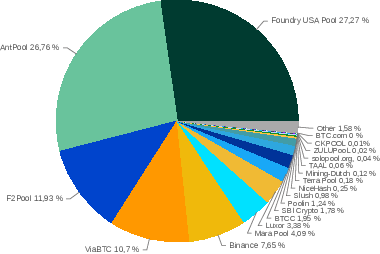
\includegraphics{chapters/img/hashrate-distribution-coin-dance-week-20231012.png}

}

\caption{Apparent BTC hash rate distribution among mining pools for the
week of October 5--12, 2023. (source: coin.dance)}

\end{figure}%

Another inherent flaw in mining is the latency associated with block
announcements. As explained in the section on the longest chain, this
latency produces orphaned blocks, which are valid but not attached to
the main chain. This means poorly connected miners have an apparent hash
rate lower than their actual hash rate.

To mitigate the effects of this flaw, miners have established
communication relays allowing them to send blocks to each other more
efficiently by removing the denial-of-service protections necessary on
the open peer-to-peer network.

The first relay was created by Matt Corallo under the name \emph{Bitcoin
Relay Network}. It was launched in 2013 and became fully operational in
2015. The network comprised several specialized nodes hosted on Amazon
Web Services infrastructure. A competitor was the Falcon network,
managed by a team from Cornell University led by Emin Gün Sirer. The
Bitcoin Relay Network was replaced in 2016 by the FIBRE
network\footnote{Matt Corallo, ``The Future of The Bitcoin Relay
  Network(s),'' July 7, 2016:
  \url{https://bluematt.bitcoin.ninja/2016/07/07/relay-networks/}.}
(Fast Internet Bitcoin Relay Engine), a network based on UDP (an
alternative protocol to TCP) that implements the \texttt{cmpctblock}
optimization, still managed by Matt Corallo. This network is used by
most miners today.

This industrialization of mining has led to centralization in both
hashing power (mining farms) and transaction selection (pools and
relays). While this aggregation is not fatal (hashers are free to leave
one pool for another, and miners are free not to use the relay), it
nonetheless reduces the chain's mining security.

Certain improvements have been proposed in mining to address this issue.
The first is the P2Pool protocol, a cooperative mining protocol based on
a peer-to-peer network of miners. It connects hashers using a
side-chain---the ``share chain''---with lower difficulty, grouping
participants' contributions. Development of P2Pool on the main Bitcoin
version appears to have been suspended in 2017. However, the process has
been implemented on Monero since October 2021 through a pool of the same
name.

The second is the Stratum V2 protocol\footnote{Braiins, ``Stratum V2
  Protocol Overview'':
  \url{https://braiins.com/stratum-v2\#job-selection}.}, which allows
(among other things) hashers to negotiate block content. While it
doesn't completely correct delegation in transaction selection, this new
version of Stratum has the merit of making the process more transparent.
As of November 2023, it was deployed only within the Braiins Pool
(formerly Slush Pool), which is behind its design.

However, these proposed improvements, while commendable, do not
eliminate the economic advantage derived from centralization, which is
also found in all industries (economies of scale). Decentralization has
a cost, justified only when the benefit it brings surpasses it---that
is, when the network is truly under attack.

\section*{An Innovative Consensus
Algorithm}\label{un-algorithme-de-consensus-novateur}
\addcontentsline{toc}{section}{An Innovative Consensus Algorithm}

\markright{An Innovative Consensus Algorithm}

To function as a distributed digital currency system, Bitcoin relies on
an innovative consensus mechanism. It involves a blockchain built by
miners, who are rewarded for their work. Each block is a timestamped set
of transactions containing a proof of work quantifying the energy
expended. Consensus is achieved by selecting the longest chain.

This consensus algorithm operates objectively, openly, and robustly,
explaining Bitcoin's success compared to its predecessors. Through its
essentially economic aspect, it provides the system with strong
resistance to opportunistic double-spending, notably thanks to the
massive mining industry supporting it.

However, there exists a more significant and insidious threat:
censorship, which we will discuss in the next chapter.

\[P = \frac{T}{\Delta t} = \frac{1}{\Delta t} \left( \frac{2^{256}}{\frac{C_{\mathrm{max}}}{d} + 1} \right)~.\]

where \(T\) is the work of a block, and
\(C_{\mathrm{max}} = \mathtt{0x00ffff} \times 256^{26}\) is the
network's maximum target value.

\bookmarksetup{startatroot}

\chapter{Resistance to Censorship}\label{ch:censure}

{[}{]} \{\#enotezch:9 label=``enotezch:9''\}

{L}\textsc{'}One of the growing issues of our time is financial
censorship. With the rise of the globalized economy, particularly
reliant on the Internet, the use of financial intermediaries has become
increasingly common. This evolution means that hindering monetary
transfers now poses a widespread complication, experienced by a growing
segment of the population.

Bitcoin offers a solution to this problem. One of its fundamental
characteristics is its resistance to censorship---that is, the
difficulty for any entity to prevent a payment from occurring. By
allowing ``online payments to be sent directly from one party to another
without going through a financial institution,'' Bitcoin bypasses the
array of financial controls that burden our modern means of payment and
savings.

Resistance to censorship, like transaction confirmation, is an economic
mechanism. It essentially relies on proof of work as applied in
Nakamoto's consensus algorithm. Consequently, alternative proposals such
as proof-of-stake algorithms exhibit much weaker resistance to
censorship.

In this chapter, we will first explore how financial censorship operates
in today's banking world and why it is likely to become more widespread
with the deployment of central bank digital currencies (CBDCs) in the
future. Then, we'll describe how censorship can be enacted within
Bitcoin and how the system can resist it. Finally, we'll explain why
alternative proposals are insufficient.

\section*{What Do We Mean by Financial
Censorship?}\label{quentendons-nous-par-censure-financiuxe8re}
\addcontentsline{toc}{section}{What Do We Mean by Financial Censorship?}

\markright{What Do We Mean by Financial Censorship?}

At first glance, the notion of censorship might seem odd when discussing
money. Commonly, censorship refers to the restriction of expression,
particularly through the prohibition of disseminating certain ideas.
However, we can understand it in a broader sense that intertwines
payment and expression.

The term ``censorship'' comes from the Latin \emph{censeo}, meaning ``to
evaluate,'' ``to estimate,'' ``to declare,'' or ``to judge.'' It
originates from a significant institution of the Roman Republic: the
censors, two magistrates tasked with conducting a census of citizens and
their property (\emph{census}), collecting taxes, supervising public
works, managing the list of those admitted to the Senate (\emph{album
senatorium}), and ensuring the maintenance of ``good morals'' among the
population by administering reprimands or temporary penalties. The
censors' first function gave rise to the term ``census.'' The second led
to concepts like ``cens'' (property assessment) and censitary suffrage.
The last function sparked what we now call censorship.

During the Middle Ages, the Latin word \emph{censura} was adopted by the
Catholic Church to take on a religious meaning, focusing solely on
speech---particularly texts. Censorship then resembled a reprimand (a
sense still sometimes used today, especially in literary criticism) or a
prohibition. It involved reviewing and correcting written works to
ensure they conformed to the dogma of the Roman Catholic Church.

However, the advent of the printing press in the 15th century disrupted
this control: the number of books exploded, diminishing the Church's
grip over publications---a control that transitioned to the State.
Consequently, censorship acquired its current political meaning,
referring to the State's examination of books, newspapers, plays, etc.,
to permit or prohibit their publication or performance. Over time, the
term came to denote any infringement on freedom of expression,
regardless of the medium, whether enacted before (a priori censorship)
or after (a posteriori censorship) dissemination.

With the rise of mass media (newspapers, radio, television) and
especially social media, the term has broadened further. Censorship now
often refers to any editorial decision made by a private entity
regarding its customers or users. While this private censorship isn't an
infringement on freedom of expression in the strictest sense, it becomes
problematic when the field is monopolized by a few actors who often
benefit from legal advantages or state subsidies. Moreover, such
censorship can directly stem from political intervention, with platforms
merely implementing government directives\footnote{For example, the
  Twitter Files revealed internal maneuvers and U.S. federal
  intervention in Twitter's censorship policies. --- Evan Perez, Donie
  O'Sullivan, Brian Fung, ``\emph{No directive: FBI agents, tech
  executives deny government ordered Twitter to suppress Hunter Biden
  story}'', \emph{CNN}, December 23, 2022:
  \url{https://edition.cnn.com/2022/12/23/politics/twitter-files-elon-musk-fbi-hunter-biden-laptop/index.html}.}.

Furthermore, censorship of expression can be executed by hindering the
economic activity of the speaker. By restricting someone's ability to
earn money and signaling that their speech is problematic, one can
compel them to silence themselves. This context gave rise to the concept
of financial censorship, defined by the international organization
\emph{Students for Liberty} as ``restricting a private entity's
financial activity to inhibit its operations, with the implicit
intention of silencing it''\footnote{Students for Liberty,
  \emph{Financial Censorship}:
  \url{https://studentsforliberty.org/blog/freedom-of-expression/financial-censorship/}.}.
The \emph{Electronic Frontier Foundation} shares this definition.

However, the repercussions of financial control extend beyond expression
and can affect human action in general. Financial censorship can thus be
understood more broadly, as adopted by three researchers from San Jose
State University who state: ``Financial censorship occurs when a
financial institution denies its services to a party because of that
party's expressed opinions, actions, or industry''\footnote{Marco
  Pagani, George Whaley, David Czerwinski, ``\emph{Frameworks for
  Assessing Financial Censorship and Its Implications}'', \emph{Journal
  of Accounting and Finance}, vol.~22, no.~1, 2022:
  \url{https://articlegateway.com/index.php/JAF/article/download/4989/4759}.}.

Finally, financial censorship can be seen as the financial restriction
itself, provided it rests on an external subjective criterion (adherence
to arbitrary norms) rather than an objective economic factor like paying
a commission. Censorship can be public (legal prohibition of a
transaction), private (by a bank, for example), or both. This definition
still embodies the idea of shaping individual behavior through financial
intervention---a meaning attributed to censorship in Bitcoin.

In general terms, financial censorship involves directly restricting an
entity's financial activities to inhibit its expression or actions. The
aim is to influence individuals by controlling the money they use, a
tool essential for their economic survival. Today, censorship primarily
targets bank credit, with transfers heavily regulated by authorities. In
the future, it could extend to digital currencies managed by central
banks.

\section*{Banking and Censorship}\label{la-banque-et-la-censure}
\addcontentsline{toc}{section}{Banking and Censorship}

\markright{Banking and Censorship}

Financial censorship operates through control over monetary transfers,
making it difficult to apply such censorship to physical cash. Cash (in
the form of precious metal coins or banknotes) enables direct,
confidential, person-to-person exchanges, preventing most restrictions
except in specific cases.

In contrast, banking involves clients holding accounts where banks
record credits and manage transfers. This setup makes financial
restrictions much easier: banks can select which transfers to process,
temporarily freeze accounts, and even refuse cash withdrawals. The same
applies to services built atop the traditional banking system, like
PayPal.

Thus, the increase in financial censorship naturally coincided with
society's bankization, which began in the 1960s in the West. This era
saw the widespread adoption of checking accounts and related payment
methods like checks, credit cards, and transfers. Over a few decades,
payments shifted to the banking sector, encouraged by law and offering
more convenience than cash---which itself faced legal restrictions. As a
result, censorship became more effective: if cash no longer allows
people to manage their affairs adequately, opting out of the banking
system is no longer viable.

This censorship was implemented through financial surveillance, now
commonplace in the banking industry. Banks are legally obligated to
monitor their clients and intervene upon detecting ``suspicious''
behavior, whether by blocking transfers or freezing accounts. They don't
do this willingly; instead, they aim to protect themselves from
potential regulatory complications, not to ``protect'' their clients.

Regulations tightened as banking became more widespread. Starting in the
1970s, combating money laundering---especially in the context of the war
on drugs---became the primary justification for imposing restrictions on
banks. In the U.S., banking regulations significantly tightened after
the Bank Secrecy Act of 1970 aimed at fighting money laundering.

With the Internet's emergence in the 1990s, international banking usage
required increased regulation. Various surveillance organizations were
established. The Financial Action Task Force (FATF), an
intergovernmental body issuing recommendations on regulatory standards
and economic sanctions, was created in July 1989 to combat money
laundering. The Financial Crimes Enforcement Network (FinCEN), a bureau
of the U.S. Department of the Treasury collecting and analyzing
financial transaction information, was established on April 25, 1990.
France's equivalent, TRACFIN (Treatment of Intelligence and Action
Against Illicit Financial Circuits), appeared in July 1990. The European
Union's first directive on preventing the use of the financial system
for money laundering dates back to June 10, 1990.

After the September 11, 2001, terrorist attacks, a new pretext emerged:
combating the financing of terrorism. In the U.S., this materialized as
the PATRIOT Act in October 2001, with Title III addressing financial
restrictions. In France, the law of November 15, 2001, on daily security
reclassified ``the act of financing a terrorist enterprise'' as an act
of terrorism itself\footnote{French Penal Code, Article 421-2-2,
  November 15, 2001.}. Financial surveillance intensified accordingly.

These developments form the foundation of what's generally known as
anti-money laundering and counter-terrorism financing (AML/CTF)
standards. This tightening is characterized by Know Your Customer (KYC)
practices, also called customer due diligence, which involve verifying
each client's identity, compliance, and associated risks. Today, this
identification requirement is integrated into all financial services.

As a result, bank secrecy---the obligation for banks not to disclose
client information to third parties---has effectively disappeared, even
in Switzerland. Using a bank account today presupposes comprehensive
transaction surveillance and meticulous scrutiny of unusual operations.
Transferring large sums without justification has become impossible.

This financial environment was summarized in January 2009 by Jonathan
Thornburg, responding to Satoshi Nakamoto on a mailing list about the
potential uses of Bitcoin:

``In the modern world, no major nation wants to allow untraceable
international financial transactions beyond a relatively modest
threshold. (Common buzzwords include `drug money laundering,' `tax
evasion,' and/or `terrorism financing.') As a result, electronic
financial transactions are currently monitored by various nation-states
and their agencies, and all but the smallest transactions are now
subject to various identification requirements for the parties at each
end''\footnote{Jonathan Thornburg, \emph{Re: Bitcoin v0.1 released},
  January 17, 2009, 16:49:45 UTC:
  \url{https://www.metzdowd.com/pipermail/cryptography/2009-January/015016.html}.}.

\section*{Instances of Financial
Censorship}\label{les-cas-de-censure-financiuxe8re}
\addcontentsline{toc}{section}{Instances of Financial Censorship}

\markright{Instances of Financial Censorship}

In recent years, notable cases of financial censorship have multiplied,
making exhaustive listing impossible. We'll highlight some prominent
examples in the West, keeping in mind that those affected often don't
publicize this censorship.

Perhaps the most well-known example is the financial blockade against
WikiLeaks, initiated by Mastercard, Visa, Western Union, Bank of
America, and others in December 2010 to silence the organization. By
October 2011, WikiLeaks reported that the blockade had cut off 95\% of
its revenue. This event had direct repercussions in Bitcoin's history,
as recounted in Chapter~\hyperref[ch:mythe]{1}.

Another case targeting specific professions was Operation Choke Point,
conducted between 2013 and 2017 by the U.S. Department of Justice. The
operation aimed to ``choke off'' certain industries by restricting their
access to credit and other banking services. Activities deemed
``high-risk'' included pawn or payday lending, gambling, pornography,
escort services, as well as the sale of tobacco, pharmaceuticals, coins,
dating services, and even travel clubs. Arms and ammunition sales were
also targeted. Defense Distributed, the libertarian crypto-anarchist
Cody Wilson's company specializing in distributing 3D-printed firearm
designs, faced account closures from Chase, PayPal, and Stripe in 2015.

In 2018, political opinions became a censorship target. Numerous
American alt-right personalities and organizations were banned from
social networks and lost access to financial services. The most
emblematic case was Alex Jones, founder of the alternative news site
InfoWars, who, besides being purged from social media in the summer of
2018, had his PayPal account closed. Other examples include the social
platform Gab (banned from PayPal, Stripe Cash App, and Coinbase), Milo
Yiannopoulos (banned from PayPal for a Nazi salute), and Robert Spencer
(blogger of the anti-Islam site Jihad Watch, ousted from Patreon under
Mastercard's pressure). In France, this censorship targeted Égalité et
Réconciliation, the association of anti-Zionist Alain Soral, which was
excluded from PayPal in August 2018 during a similar purge. The
association also saw multiple bank accounts (Banque Postale, BNP
Paribas, Banque Populaire) closed over the years.

In the political realm, but in China, the movement against the Hong Kong
government's proposed extradition law amendment---from March 2019 to
July 2020---faced interventions from the international banking giant
HSBC, likely under pressure from the central Chinese government. In
November 2019, HSBC's Hong Kong subsidiary closed an account used to
support the protest movement. Then, in December 2020, it froze the
account of democrat Ted Hui. By 2023, it emerged that HSBC was denying
Hong Kongers who fled to the UK access to their pension funds, totaling
£2.2 billion.

More recently, the COVID-19 pandemic provided additional examples of
financial censorship. Activists opposing measures like lockdowns, mask
mandates, and mandatory vaccinations faced extensive censorship, often
accused of spreading misinformation. The Dutch action group
Viruswaarheid---opposing social distancing, lockdowns, curfews, and
vaccination programs---had its donation-receiving bank account closed by
ING Bank in February 2021.

A standout event is the Canadian ``Freedom Convoy'' of February 2022,
initiated by truckers protesting mandatory vaccinations for cross-border
travel. They converged on Ottawa to express their discontent. The
movement encountered severe financial censorship. Initially,
crowdfunding platforms canceled campaigns intended to support the
truckers' journey: GoFundMe withdrew a campaign that had raised 10
million Canadian dollars on February 4; funds raised through campaigns
on the Christian platform GiveSendGo (around 9 million dollars) were
frozen by the Ontario government and couldn't be distributed. Financial
repression escalated when, following the state of emergency declared by
Justin Trudeau on February 14, the Canadian government froze personal
and business bank accounts linked to the movement: 280 accounts
containing a total of 8 million dollars were frozen. The following year,
Judge Paul Rouleau, heading the Commission on the State of Emergency,
stated that freezing bank accounts was a ``powerful tool to discourage
participation {[}in the protests{]} and encourage protesters to
leave''\footnote{Rob Gillies, ``\emph{Judge: Canada right to invoke
  emergency act in truck protest}'', \emph{Associated Press News},
  February 17, 2023:
  \url{https://apnews.com/article/canada-government-justin-trudeau-ottawa-montana-9c1e37aa86d4315703e69f7794637e7f}.}.

Another significant event was the tightening of economic sanctions
against Russia by Western states following its invasion of Ukraine in
February 2022. Financial sanctions included excluding certain Russian
banks from the SWIFT system, prohibiting financing in Russia and the
purchase of rubles, and banning the provision of wallet, account, or
custody services for crypto-assets. Generally, transfers to Russia were
prohibited, preventing exiled Russian citizens from sending money to
their families. This also affected Ukrainians whose relatives remained
in territories occupied by the Russian army, such as a Ukrainian woman
in France unable to send a 100-euro bank transfer to her parents in
Donetsk.

In the West, financial measures were also taken to enforce censorship of
Kremlin-funded media. In January 2023, RT France, already banned from
broadcasting in Europe but still accessible online, had its assets
frozen, forcing it to close permanently.

Lastly, in discussing financial censorship instances, we must mention
activities related to cryptocurrencies, which continue to face
restrictions from financial institutions. Banks regularly impede
cryptocurrency purchases by prohibiting clients (claiming to ``protect''
them) from sending funds to exchanges. Additionally, companies in the
sector often struggle to open bank accounts due to traditional
institutions' mistrust\footnote{In \emph{Cryptocurrency: The New War},
  François-Xavier Thoorens recounts how he and his family were expelled
  from their long-standing bank after attempting to open a professional
  account to receive funds from Ark's ICO (pp.~91--97). His experience
  isn't unique.}.

Financial censorship is increasingly prevalent in our society. It
affects many individuals across political spectrums, nationalities, and
professions. Often enacted without specific legal decisions, it imparts
a hidden, arbitrary nature to the exertion of real power, making it a
subtle and challenging issue to articulate.

The intensification of this censorship drives people to explore Bitcoin.
Experiencing such restrictions naturally leads individuals to seek ways
to circumvent them, even if minor. When people grasp censorship as a
concrete reality rather than an abstract risk, they feel compelled to
liberate themselves and safeguard against this danger, highlighting (or
reaffirming) Bitcoin's value proposition\footnote{Nick Szabo described
  this effect on Peter McCormack's podcast in 2019: ``Some people need
  to be hit by reality. When you're censored by a bank---which happens
  increasingly---and people start realizing they can silence political
  enemies through banks, they become Bitcoin fans.'' --- \emph{What
  Bitcoin Did Podcast}, \emph{Nick Szabo on Cypherpunks, Money and
  Bitcoin}, November 1, 2019:
  \url{https://www.whatbitcoindid.com/podcast/nick-szabo-on-cypherpunks-money-and-bitcoin}.}.
This was the case for the author of this book, whose bank account was
frozen without notice or explanation, only regaining access to his funds
six months later.

\section*{Censorship and Central Bank Digital
Currency}\label{censure-et-monnaie-numuxe9rique-de-banque-centrale}
\addcontentsline{toc}{section}{Censorship and Central Bank Digital
Currency}

\markright{Censorship and Central Bank Digital Currency}

The trend is clear: with the widespread use of bank accounts over cash,
the power of financial censorship has grown significantly. While this
censorship remains occasional today, we can anticipate it becoming a
more pressing issue in the future, especially with the gradual
deployment of central bank digital currencies (CBDCs) and the concurrent
decline of physical cash.

As discussed in the section on central bank digital currencies in
Chapter~\hyperref[ch:adversaire]{4}, digitizing money is the next step
in state-issued currency evolution. Since 2016, central banks worldwide
have been designing systems usable by the general public, with
communications on the subject increasing since 2020.

Such digital currencies would allow for additional seigniorage income by
eliminating cash production costs and reclaiming monetary activities
currently facilitated through credit issued by commercial banks. More
pertinent here, they would enable total financial control over citizens'
transactions by centralizing system management within the central bank
and accredited organizations.

This control would naturally come with enhanced financial surveillance,
justified by familiar pretexts like combating money laundering and
terrorism financing. This could lead to a panoptic system where
surveillance occurs without the subject's awareness. Central banks deny
intentions to move in this direction, but they will never make their
systems entirely confidential, always reserving oversight rights for
competent authorities.

Financial surveillance could be reinforced by the gradual disappearance
of cash, already underway in some parts of the world. In Sweden,
discussions about ending cash are active, with the state promoting
innovative digital payment methods. In China, most transactions occur
through mobile payment systems like WeChat Pay and Alipay. It's no
coincidence that these two countries were among the first to seriously
consider developing a digital currency.

The war on cash manifests in some countries through demonetizing certain
circulating bills, which can be exchanged for other bills or deposited
into bank accounts upon proof of fund origin. In November 2016, India's
government, led by Narendra Modi, demonetized 500 and 1,000 rupee notes
(worth approximately \$7.50 and \$15), constituting 86\% of currency in
circulation, aiming to combat counterfeit banknotes, tax evasion, and
the informal economy. In early 2023, Nigeria attempted a similar move by
limiting withdrawals and demonetizing large denominations to control
inflation, fight counterfeiting, and promote the electronic naira
(eNaira) launched by the central bank in October 2021. Such
demonetization isn't new; post-World War II Europe saw similar actions
to curb inflation and eliminate black-market profits, leading the
character Le Dabe in \emph{The Counterfeiters of Paris} to remark,
``When it comes to money, states have all the rights, and individuals
none!''

With digital currency in place and cash significantly restricted,
law-abiding citizens would have no choice but to use this surveilled
system. The system could limit spending amounts, dictate usage purposes,
and control trading partners. Moreover, being a computerized system, it
could easily be programmed to impose spending conditions on users'
funds. Such programmability would allow authorities to steer
individuals' political, economic, and moral behaviors in desired
directions, giving financial censorship unprecedented reach.

Economically, this could enhance what central bankers call monetary
policy transmission---the process by which monetary policy decisions
affect the broader economy and price levels. Currently, this
transmission primarily operates through adjusting key interest rates. In
the future, it could involve programming the currency itself,
transforming social aid systems into direct subsidies requiring rapid
spending in specific economic sectors to stimulate them.

Morally, such programmability could massively influence people's words
and actions. In our modern society, this might occur under the guise of
combating climate change by rewarding ``eco-friendly'' behaviors (like
renting bikes) and penalizing ``polluting'' ones (like consuming meat).
This suggests the potential establishment of a Chinese-style social
credit system.

Politically, this system could suppress opposition by penalizing those
with dissenting thoughts, outspoken critics, or protesters. Authorities
could strengthen their position by enforcing measures not through public
and legal avenues (aligned with the concept of the rule of law), but via
covert and discretionary means. This could usher in the beginnings of a
totalitarian regime where the state knows all, controls all, and formal
laws become unnecessary. The CBDC would serve as a powerful tool for
mass financial surveillance, potentially paving the way for an Orwellian
future where individuals lack privacy and have minimal ability to resist
authority.

Such widespread financial censorship would be unprecedented.
Implementing it manually would be challenging, necessitating delegation
to algorithms equipped with artificial intelligence to detect and
instantly block undesired transactions. The CBDC system could lead us
toward a scenario reminiscent of Saint John's description in the
\emph{Book of Revelation}:

``By these means, all people, great and small, rich and poor, free and
slave, will receive a mark on their right hands or on their foreheads,
so that they cannot buy or sell unless they have the mark---the name of
the beast or the number of its name''\footnote{Revelation 13:16--17.}.

In this dystopian world, whose ramifications we can scarcely imagine,
hope would be embodied by Bitcoin, whose fundamental promise is to
escape such interventions. Through its resistance to censorship, Bitcoin
would serve as an oasis of freedom amid widespread servitude.
Essentially, it would be the last refuge for a population ensnared by
technological subjugation.

\section*{Censorship in Bitcoin}\label{la-censure-dans-bitcoin}
\addcontentsline{toc}{section}{Censorship in Bitcoin}

\markright{Censorship in Bitcoin}

To understand how Bitcoin opposes censorship, we must examine how
censorship can be applied to the blockchain. While the Nakamoto model is
reputed to be \emph{resistant} to censorship, this doesn't mean it's
``uncensorable.'' Censorship in Bitcoin is not only possible but also
likely beyond a certain adoption stage.

In the context of Bitcoin, ``censorship'' specifically refers to the
action of preventing a transaction from being executed on an
economically irrational basis by hindering its permanent inclusion in
the blockchain. This definition aligns with the idea of restricting an
entity's financial activity to shape its behavior. In a sense, this
censorship resembles speech censorship, as it indirectly prevents an
individual from recording a signed transaction in a ledger.

Censorship in Bitcoin can be extrapolated from existing practices in the
banking world and the cryptocurrency sector, beginning with the
justifications used to defend it. On one hand, traditional finance's
reasons apply to Bitcoin: combating money laundering, terrorism
financing, and protecting investors---since cryptocurrency can
facilitate tax evasion, fund various projects, and partake in scams. On
the other hand, new pretexts emerge, such as preventing local currency
devaluation (a deflationary instrument poses unfair competition) or
combating climate change (mining emits CO₂).

Authorities derive general regulations from these pretexts, applied
internationally, as seen in the global banking system. Different
jurisdictions base their policies on FATF recommendations, primarily
aimed at fighting money laundering and terrorism financing. As discussed
regarding jurisdictional arbitration (see
Chapter~\hyperref[ch:adversaire]{4}), countries are strongly encouraged
to implement these recommendations to avoid economic sanctions from
member states. The IMF can also be leveraged, aiming to ensure global
monetary system stability (thus protecting member states' currencies).

This cooperation enables the creation of blacklists of addresses
non-compliant with regulations, distributed to various regulated
financial actors. Examples include lists compiled by the Office of
Foreign Assets Control (OFAC), a U.S. Treasury agency enforcing
international financial sanctions, which wields significant influence
due to the extraterritoriality of U.S. law.

Censorship already exists within parts of the Bitcoin economy. Regulated
entities block bitcoins (and other cryptocurrencies) from blacklisted
addresses and freeze user accounts until they provide explanations.
However, this practice remains partial and implicit: transactions
themselves aren't explicitly prohibited yet, but funds must not be sent
to regulated financial intermediaries like exchanges or payment
processors. This situation pushes some platforms to overcompensate by
rejecting bitcoins originating from coin mixers and freezing accounts of
users engaging in such activities, even without explicit
regulations\footnote{On Ethereum, addresses linked to the Tornado Cash
  mixer contract were blacklisted by OFAC in August 2022. On BTC, no
  explicit laws or lists related to mixing exist---only general
  suspicion.}.

Regulations can also extend to the mining industry. Mining naturally
tends toward centralization through hash power aggregation in mining
farms, miners joining pools, and pools using communication relays. These
large entities are often identifiable and more likely to comply with
transaction-processing regulations, potentially leading to network
censorship.

Miners might initially practice passive censorship by systematically
refusing to confirm certain transactions for economically irrational
reasons, typically under regulatory pressure. This type of censorship
was considered by Marathon Group's pool in 2021, which announced plans
to practice ``clean block mining''\footnote{Marathon Patent Group and
  DMG Blockchain Solutions announced plans for ``clean block mining'' in
  January 2021 before retracting under public pressure. --- Archived
  press release:
  \url{https://web.archive.org/web/20210128112455/https://www.marathonpg.com/news/press-releases/detail/1220/marathon-patent-group-and-dmg-blockchain-solutions-to-form}.}
before retracting under public pressure. On Ethereum, this filtering
occurs with validators using MEV-boost relays complying with OFAC
standards, excluding transactions deemed illicit\footnote{Maximal
  Extractable Value (MEV), initially called Miner Extractable Value, is
  the maximum value a validator can generate by reordering or excluding
  transactions in their block. As of October 2022, over 50\% of Ethereum
  transactions passed through MEV-boost relays complying with OFAC
  standards. --- See MEV Watch: \url{https://www.mevwatch.info/}.}. As
of 2023, participants in these relays were primarily exchanges.

Passive censorship isn't overly problematic since it requires 100\%
compliance by miners to be effective. Dissident miners---those
deliberately ignoring regulations---can validate ignored transactions,
mitigating the impact. Only confirmation times might be affected.

The situation becomes more severe if compliant miners (strictly adhering
to regulations) start rejecting blocks containing ``illicit''
transactions. This active censorship involves preventing transactions
from being confirmed by orphaning any blocks that include them.
Sustaining this requires majority control of the network's hash
power---essentially a 51\% attack. The weaker branches formed by the
censorship attack are abandoned due to the longest-chain rule, as
illustrated in Figure~\hyperref[fig:censorship-attack]{9.1}.

\begin{figure}

{\centering 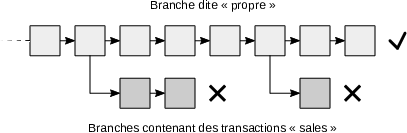
\includegraphics{chapters/img/mining-attack-censorship.png}

}

\caption{Active Censorship Attack.}

\end{figure}%

Such an attack's cost can be colossal, depending on the hash power
deployed\footnote{As discussed in Chapter~\hyperref[ch:confirmation]{8},
  such an attack costs billions on Bitcoin's main network.}. However,
this cost might be justified by the suppression of activities avoiding
taxes and seigniorage. As discussed in
Chapter~\hyperref[ch:adversaire]{4}, the typical attacker is the state,
whose extraction power heavily relies on monetary control---it may not
mind reducing (or destroying) Bitcoin's utility to achieve its goals.

This hypothetical attack would likely be preceded by a declaration of
war against Bitcoin. Tolerance toward users would vanish, and unofficial
activities would become official targets: all transactions not
explicitly authorized would be declared illegal. Free usage would be
criminalized, and honest mining would be targeted.

Such a crackdown would help co-opt more mining pools, transmitting state
directives to them. The state could also requisition or purchase its own
mining hardware, eventually amassing majority hash power. With
sufficient power, the attack would commence.

Active censorship is insidious because only 51\% compliance is needed
for enforcement. Prolonged over time, it could establish a new norm.
Economically rational miners might be incentivized to comply with
censorship, as Juraj Bednar discussed\footnote{Juraj Bednar,
  ``\emph{Bitcoin censorship will most likely come, pt 2}'', November
  18, 2020:
  \url{https://juraj.bednar.io/en/blog-en/2020/11/18/bitcoin-censorship-will-most-likely-come-pt-2/}.}.
The attacker doesn't necessarily need to maintain majority hash power
indefinitely.

Privacy doesn't prevent censorship but increases its cost. If all users
refuse to comply with surveillance norms, censors would have to reject
all transactions, forfeiting corresponding fees. The attack would
effectively entail destroying the blockchain's utility by mining empty
blocks---a Goldfinger attack, named after the antagonist in the 1964
James Bond film who sought to irradiate the U.S. gold reserve at Fort
Knox to render it unusable and inflate the value of his own
gold\footnote{Joshua A. Kroll, Ian C. Davey, Edward W. Felten,
  ``\emph{The Economics of Bitcoin Mining, or Bitcoin in the Presence of
  Adversaries}'', \emph{Workshop on the Economics of Information
  Security}, 2013:
  \url{https://www.cs.princeton.edu/~felten/writing/bitcoin-in-the-presence-of-adversaries.pdf}.}.

Thus, censorship in Bitcoin is possible. However, it's neither easy nor
definitive, thanks to a protocol mechanism designed to combat such
attacks: resistance to censorship.

\section*{The Mechanism of Resistance to
Censorship}\label{le-muxe9canisme-de-ruxe9sistance-uxe0-la-censure}
\addcontentsline{toc}{section}{The Mechanism of Resistance to
Censorship}

\markright{The Mechanism of Resistance to Censorship}

Resistance to censorship refers to the difficulty of arbitrarily
obstructing transactions. It's commonly cited as one of Bitcoin's key
promises: allowing anyone to send funds to anyone else, anytime,
anywhere, provided they have Internet access.

Resistance to censorship is crucial for Bitcoin. Without it, the system
couldn't survive as it would become a centrally controlled platform,
with an authority deciding which transactions are acceptable. It would
need to adapt (like GoldMoney or PayPal) or perish (like e-gold or
Liberty Reserve). Moreover, absolute control over transaction selection
would allow such an authority to exert irresistible influence over the
protocol through soft forks (as we'll explore in
Chapters~\hyperref[ch:changement]{10}
and~\hyperref[ch:determination]{11}), ultimately destroying the original
monetary policy. Without resistance to censorship, Bitcoin's value
proposition collapses.

However, Satoshi Nakamoto never explicitly described this resistance. In
his communications, he explained how his system was economically secured
against double-spending---a significant advancement over previous
decentralized models---but didn't elaborate on opposing censorship,
i.e., partially or entirely blocking transactional activity by a hostile
entity. He seemed to rely on the goodwill of ``honest'' miners, even
suggesting there would ``probably always be nodes willing to process
transactions for free''\footnote{Satoshi Nakamoto, \emph{Bitcoin v0.1
  released}, January 8, 2009, 19:27:40 UTC:
  \url{https://www.metzdowd.com/pipermail/cryptography/2009-January/014994.html}.},
implying resistance was a given.

The mechanism of resistance to censorship was highlighted in 2018 by
developer and author Eric Voskuil, who showed it fundamentally relies on
transaction fees\footnote{Eric Voskuil initially described the
  censorship resistance mechanism in January 2018:
  \url{https://github.com/libbitcoin/libbitcoin-system/wiki/Other-Means-Principle/77d7556a14f89d1704f1bb97ca0aed04606363d0}.
  See also Eric Voskuil, ``Censorship Resistance Property,'' in
  \emph{Cryptoéconomie: Fundamentals of Bitcoin}, Amazon KDP, 2022,
  pp.~24--25.}. Similar to resistance against double-spending,
resistance to censorship isn't absolute but economic: regulation funded
by fees from prohibited transactions.

Mining security hinges on a majority principle: the computing power
controlled by honest miners must exceed that of attackers. The crucial
factor isn't the highest possible hash rate but that miners with
significant power are willing to mine all transactions paying
appropriate fees and consistently build on the longest chain.

Thus, security isn't solely dependent on hash power. It also involves
the distribution of that power and the proportion of miners relative to
the broader population\footnote{Eric Voskuil, ``Qualitative Security
  Model,'' in \emph{Cryptoéconomie: Fundamentals of Bitcoin}, Amazon
  KDP, 2022, pp.~59--62.}. A hash rate concentrated in a single miner's
hands would offer security equivalent to a centralized system, dependent
on that miner. Conversely, a widely distributed network with substantial
hash power may face co-option risks if it comprises few miners compared
to one with many.

The solution to censorship lies with dissident miners willing to confirm
contentious or illegal transactions. The risks these miners face must be
economically compensated.

Dissident miners need anonymity to mine clandestinely. This is ensured
as miners aren't required to identify themselves within the protocol.
Reporting mined blocks by pools is optional and voluntary, intended to
reassure users about network distribution.

The portion of mining revenue from new coin creation plays a minor role
in combating censorship, whether passive or active. This reward is
identical for all miners, so it doesn't influence their economic choice
to include or exclude transactions. Furthermore, potential utility loss
(and thus mining revenue) from active censorship (an attack) wouldn't
deter the authority aiming to achieve control or destruction by
dictating permissible transactions.

In contrast, transaction fees are crucial to the resistance mechanism.
Integrated into the protocol, these fees are publicly associated with
each transaction. They counter passive censorship by incentivizing
miners to confirm transactions and deter active censorship by enhancing
the economic weight of the censored branch.

In an active censorship attack, censors obtain over half the network's
computing power and openly reject certain transactions (e.g., via a
blacklist) by refusing blocks containing them. The censors' chain is
considered valid by honest nodes due to its length.

Here, the fee mechanism plays a role. Users of censored transactions,
noticing delays, increase their fees---a natural response observed
during network congestion, like during the 2017 bubble when median
transaction fees exceeded \$30. It's logical to pay higher fees to
transfer large sums, which carry more risk than small
transfers\footnote{While Bitcoin fees are currently based on data size
  or transaction weight, heightened censorship threats might prompt
  users to pay fees proportional to transfer amounts, as in traditional
  finance.}.

This increase generates additional fees---the difference between fees
from all transactions and those from unauthorized transactions in honest
nodes' mempools. This surplus incentivizes dissident miners to deploy
more hash power over time: the larger the suppressed economy, the
greater the resulting hash power differential.

Dissident miners coordinate privately or signal to plan a response. Once
sufficient hash power is gathered, they begin confirming censored
transactions. With majority power, their chain becomes the longest,
invalidating the censors' chain. Thus, censorship is overcome---at least
until the next attack.

Therefore, the resistance mechanism is deeply embedded in the protocol.
Proof of work, anonymous mining, and the integrated fee system
collectively enable coordinating a fee market to repel censors. While we
can't guarantee Bitcoin's uncensorability---given unknowns like the
censored economy's size, attack scale, or users' willingness to pay
fees---the mechanism remains functional.

Notably, the role of transaction fees, elucidated by Eric Voskuil in
2018, has been overlooked by some crypto-economic protocols. Ethereum,
for instance, opted to burn a portion of network fees to make ether
deflationary with EIP-1559's activation in August 2021. The Ethereum
community also transitioned to proof of stake in September 2022, marking
another step toward accepting censorship, as we'll explain later.

\section*{The Importance of
Privacy}\label{limportance-de-la-confidentialituxe9}
\addcontentsline{toc}{section}{The Importance of Privacy}

\markright{The Importance of Privacy}

Financial censorship closely aligns with transaction surveillance. Such
surveillance refines transaction selection, allowing subtle control over
the economy without alarming compliant individuals. This applies to both
traditional banking and Bitcoin.

Protecting one's wealth and freedom can be approached in two ways:
physical defense and concealment. Physical defense involves directly
safeguarding property (possibly with firearms) or indirectly through
state police or private security services---a common choice among the
wealthy. While effective against common criminals, it's less so against
the dominant local power---the state.

Consequently, individuals often opt for concealment, hiding their wealth
to prevent others from seizing it directly. This deters aggressors
relying on threats of violence, as extracting information incurs
additional costs proportional to resistance.

This method ties directly to privacy---the act of restricting
information to a select few. Privacy differs from secrecy in that one
can choose to reveal information selectively. In financial contexts,
this means ensuring transaction details are known only to participants.

Privacy underpins individual freedom in society and is essential for
everyone. It creates an asymmetry between the weak and the strong, the
individual and the state, preventing absolute encroachment on individual
rights. States may argue otherwise, suggesting those with nothing to
hide have nothing to fear\footnote{``I say that anyone who trembles now
  is guilty; for innocence never fears public scrutiny.'' --- Maximilien
  de Robespierre, \emph{Speech of 11 Germinal, Year II}, March 31, 1794.},
but history---especially 20th-century totalitarian regimes---proves this
false.

Thus, because financial censorship originates from state initiatives,
resistance to censorship is intrinsically linked to privacy.

On one hand, individual resistance to censorship relies on system
privacy. If the state knows all transactions, it can penalize users for
unauthorized transactions, even if confirmed by the network. Some BTC
proponents highlight protocol transparency as an advantage over opaque
banking systems, emphasizing pseudonymity and reserving anonymity for
privacy-focused cryptocurrencies like Monero. However, this
misunderstands transparency's role: in Bitcoin, data is public solely to
ensure consensus and auditability; Monero simply implements a different
transparency compromise.

On the other hand, user privacy depends on the system's resistance to
censorship. If the state controls transaction selection, it can choose
to confirm only transactions revealing sender and recipient identities.
Some Monero advocates argue that default system privacy protects users
from censorship, as the state can't censor unknown transactions.
However, this view is naive, as users can technically disclose
address-related information to surveillance authorities\footnote{In
  Monero and similar systems, disclosing transactions linked to an
  address involves using a private view key.}; the main barrier is the
additional cost such surveillance entails.

Therefore, privacy and resistance to censorship are interdependent in
Bitcoin. Without privacy, individual resistance to censorship falters;
without resistance to censorship, individual privacy erodes.
Consequently, widespread surveillance poses a significant threat.

Surveillance has expanded in Bitcoin alongside its economic growth,
through regulation of financial intermediaries. Cryptocurrency exchanges
have been compelled to implement KYC and AML standards akin to
traditional banking. This information gathering has fostered blockchain
analytics firms like Chainalysis and CipherTrace, which cross-reference
identification data with blockchain events to derive probable
interpretations, providing results to clients like state agencies and
financial institutions. The net tightens further with adaptations of the
``Travel Rule'' recommended by the FATF and enforced by entities like
Switzerland's FINMA, requiring intermediaries to verify withdrawal
addresses\footnote{The Travel Rule, originating from the U.S. FinCEN in
  1996, requires financial institutions to transmit sender information
  during certain transfers. The FATF extended this to ``virtual assets''
  in June 2019. In the crypto context, it could involve integrating
  Address Ownership Proof Protocol (AOPP) into wallets.}.

This evolution poses a substantial threat to Bitcoin. In response,
efforts to thwart surveillance have emerged, including privacy-enhancing
techniques like coin mixing (CoinJoin) and methods integrated into
Monero. We'll delve into this in Chapter~\hyperref[ch:rouages]{12}.

In summary, privacy is vital for preserving wealth and autonomy. True
freedom demands protecting one's private life. As the writer Florian
aptly noted: ``To live happily, live hidden''\footnote{Jean-Pierre
  Claris de Florian, ``The Cricket,'' in \emph{Fables de Florian}, 1793.}.

\section*{Human Interventions in
Consensus}\label{les-interventions-humaines-dans-le-consensus}
\addcontentsline{toc}{section}{Human Interventions in Consensus}

\markright{Human Interventions in Consensus}

The possibility of censorship in Bitcoin often inspires a search for
solutions, reflecting the engineer mindset common among cryptocurrency
enthusiasts. Many are drawn to alternatives to fee-based regulation:
direct human intervention on the blockchain. This involves leveraging
``social consensus,'' or the protocol's determination mechanism. Two
ideas gaining traction are anti-censorship UASF (User Activated Soft
Fork) and proof-of-work change UAHF (User Activated Hard Fork). However,
we'll argue that this temptation is dangerous.

The first idea is to reject censorship by invalidating the censors'
chain partially or entirely, violating the longest-chain principle. This
can be achieved by rendering censors' blocks invalid or enforcing the
validity of an alternative chain via a temporary checkpoint. Such
measures constitute a soft fork (a restriction of consensus rules) and
require user activation at a specific timestamp or block height, hence a
UASF. This approach causes a split, as it lacks majority hash power
support in censorship scenarios.

The concept of invalidating censorship through social consensus was
discussed by Vitalik Buterin in 2016 regarding proof of stake:

``On medium to long time scales, humans are quite good at consensus.
Even if an attacker had unlimited hash power and managed a 51\% attack
against a major blockchain, reversing even just the last month of
history, convincing the community of the new chain's legitimacy would be
much harder. They'd need to compromise block explorers, trusted
community members, major media outlets, and more---convincing the world
their chain came first. These social considerations ultimately protect
any blockchain in the long term, whether the community admits it or not
(note that Bitcoin Core acknowledges the primacy of the social
layer)''\footnote{Vitalik Buterin, ``\emph{A Proof of Stake Design
  Philosophy}'', December 30, 2016:
  \url{https://medium.com/@VitalikButerin/a-proof-of-stake-design-philosophy-506585978d51}.}.

This measure can be implemented through direct invalidation, but it's
feasible only if censors mark their blocks in some way. This was done by
Bitcoin ABC on December 1, 2020, to counter an active censorship attack
from a disgruntled miner following a split with Bitcoin Cash\footnote{Only
  one block (662,687) from the attacker was invalidated, discarding 172
  blocks and making the uncensored chain valid. --- Nikita Zhavoronkov
  on Twitter, December 1, 2020:
  \url{https://twitter.com/nikzh/status/1333893457920876550}.}.

Alternatively, checkpoints can be incorporated into the
protocol---blocks deemed valid by default. This mechanism was added to
Bitcoin software in July 2010 to prevent deep reorganizations; some
checkpoints remain in Bitcoin Core\footnote{The latest checkpoint is
  block 295,000 mined on April 9, 2014. See the chainparams.cpp file in
  Bitcoin Core.}. By enforcing a specific block, censors' chains can be
invalidated. Bitcoin SV employed this in August 2021 amid active
censorship\footnote{BSV Association on Twitter, September 3, 2021:
  \url{https://twitter.com/BitcoinAssn/status/1422668065024663554}.}.

While such interventions might offer temporary relief, they don't
provide robust censorship resistance. Relying on social agreement for
consensus introduces instability. It opens the door for hostile entities
to destabilize the system by sowing discord within the community (e.g.,
pressuring influencers), leading to splits that can't be objectively
resolved.

Direct human intervention in transaction confirmation is thus
ill-advised. Even if participants agree on the undesirability of an
event, they often disagree on handling it, as seen in the Ethereum and
Ethereum Classic split. Humans can reach consensus long-term, as
evidenced by convergence in languages, religions, currencies, etc.
However, short-term consensus is unlikely, necessitating automated
mechanisms like mining.

Another proposed measure, less subjective but more disruptive, is
altering the proof-of-work function. This would halt an attack by
rendering censors' specialized hardware obsolete, inflicting financial
loss. It's a hard fork (incompatible consensus rule change) requiring
user activation---a UAHF. This extreme option was supported by
developers like Luke-Jr and Gregory Maxwell during the block size debate
(2015--2016) and defended by Bitcoin ABC's lead developer Amaury Séchet
in November 2018, calling it a ``nuclear option of last
resort''\footnote{Amaury Séchet (deadalnix) on Twitter, November 12,
  2018: \url{https://twitter.com/deadalnix/status/1061947426096009216}.}.

Like invalidating censorship through social intervention, this route is
more harmful long-term than maintaining the status quo. Firstly, losses
incurred by censors also affect honest and dissident miners. Secondly,
the economy splits between two chains, reducing overall utility.
Thirdly, attack costs decrease short-term. Fourthly, miners lose
protocol confidence, necessitating risk hedging against future changes,
raising security costs. Lastly, the new mining distribution may not
improve over the old, as large miners can deploy capital more
efficiently.

Overall, short-term human intervention is undesirable. If the chain
faces a mining attack, it's likely under social attack too.
Interventions may multiply, leading to spiraling splits and economic
insignificance. The case of Bitcoin Cash illustrates this: due to
biannual hard forks, it underwent two major splits post-separation from
Bitcoin-BTC (in 2018 with BSV and in 2020 with XEC), collectively valued
at less than 1\% of BTC's aggregate value. Such risks are magnified for
a mature Bitcoin supporting a large, diverse economy.

\section*{Variants of Proof-of-Work
Consensus}\label{les-variantes-des-consensus-par-preuve-de-travail}
\addcontentsline{toc}{section}{Variants of Proof-of-Work Consensus}

\markright{Variants of Proof-of-Work Consensus}

Censorship risks have inspired alternative consensus algorithms to
Nakamoto's. The most notable is proof of stake, discussed in the next
section. Other alternatives modify the proof-of-work algorithm, with
three main variants: merged mining, proof of space, and early
finalization.

The first is merged mining---simultaneously mining multiple chains by
reusing work from a parent chain to validate auxiliary chains.

Satoshi Nakamoto described this in December 2010 regarding BitDNS (the
precursor to Namecoin). He wrote:

``I think it's possible for BitDNS to be a completely separate network
and have its own blockchain, yet share proof-of-work with Bitcoin. The
only overlap would be miners able to search for proof-of-work for both
networks simultaneously.

Networks wouldn't need coordination. Miners would run both networks in
parallel, hashing in such a way that solutions solve both. A solution
might apply to only one network if difficulties differ.

An external miner could call `getwork' on both programs and combine the
work.

Rather than fragmenting effort, networks would share and increase total
computational power. This solves the issue of multiple networks
endangering each other if computational power concentrates on one.
Instead, all networks share combined power, making it easier for smaller
networks to launch by tapping into existing miners''\footnote{Satoshi
  Nakamoto, \emph{Re: BitDNS and Generalizing Bitcoin}, December 9,
  2010:
  \url{https://bitcointalk.org/index.php?topic=1790.msg28696\#msg28696}.}.

Merged mining reuses partial proof-of-work from a parent chain as valid
for an auxiliary chain. These auxiliary proofs (AuxPoW) are mining
byproducts requiring no additional energy---only management of the
auxiliary chain.

Auxiliary chain miners receive extra rewards from local coin creation
(if using a new unit) and transaction fees, incentivizing parent chain
miners to participate. This allows auxiliary chains to quickly gain
significant hash rates.

Merged mining facilitates bootstrapping new cryptocurrencies by
leveraging established mining industries. It has been implemented with
Namecoin (relative to Bitcoin) and Dogecoin (relative to Litecoin). It's
also suggested for sidechain synchronization, as in RSK's hybrid
implementation, and considered in Paul Sztorc's Drivechain proposal (see
Chapter~\hyperref[ch:scalabilite]{14}).

However, merged mining's security benefits over classic mining are
limited. While it increases participants and restricts attackers (to
parent chain miners), attack costs remain tied to the auxiliary chain's
mining revenue and, in censorship cases, transaction fees.

An illustrative example is Coiledcoin (CLC), an alternative
cryptocurrency launched in January 2012, which suffered a fatal
censorship attack soon after. Bitcoin developer Luke-Jr executed the
attack via his mining pool Eligius without informing miners. He noted
that no pool members suffered losses---the main cost was his time
configuring software\footnote{Luke-Jr, \emph{Re: {[}DEAD{]} Coiledcoin -
  yet another cryptocurrency, but with OP\_EVAL!}, January 6, 2012:
  \url{https://bitcointalk.org/index.php?topic=56675.msg678006\#msg678006}.}.

Merged mining affects parent chain mining security by artificially
increasing block mining power, seemingly beneficial but ineffective
against transaction censorship. It also centralizes mining due to the
burden of managing auxiliary chains: if they become economically
significant, parent chain miners must mine them to remain profitable.

The second alternative is proof of space (or capacity/storage), based on
memory storage rather than computing power---the resource is disk space.

This idea has partially appeared in hybrid proof-of-work algorithms to
deter specialized hardware (ASICs) and favor general hardware (CPUs,
GPUs). Examples include the scrypt function in Tenebrix (inherited by
Litecoin), Ethereum's former Ethash algorithm, and Monero's RandomX.

Pure proof-of-space algorithms exist, such as Chia Network's system by
Bram Cohen, using ``proofs of space and time'' to determine the correct
chain.

These algorithms aim to enhance censorship resistance by encouraging
broader participation, improving validation distribution. However, they
merely shift the problem. Proof of space still involves external energy
expenditure, resembling proof of work. Optimization remains possible at
hardware (ASICs) and industrial levels (economies of scale), so
centralization pressures persist. The goal becomes aligning specialized
hardware efficiency with universally used tools, as RandomX attempts
with CPUs.

The third alternative is early block finalization---implementing moving
checkpoints to consider blocks below a certain depth as final. Vitalik
Buterin describes this as ``weak subjectivity''\footnote{Vitalik
  Buterin, ``\emph{Proof of Stake: How I Learned to Love Weak
  Subjectivity}'', November 25, 2014:
  \url{https://blog.ethereum.org/2014/11/25/proof-stake-learned-love-weak-subjectivity}.}.

Bitcoin ABC introduced such an algorithm on November 20, 2018, in
Bitcoin Cash, to counter threats from Bitcoin SV, considering blocks
final after 11 confirmations. This persists in some Bitcoin Cash and XEC
implementations and is enforced by major exchanges, making it a de facto
consensus rule.

Ethereum Classic, after multiple double-spend attacks in 2019 and 2020,
integrated a variant called Modified Exponential Subjective Scoring
(MESS) on October 11, 2020. MESS assigns different scores to competing
branches, favoring earlier-seen segments. It purportedly reduces attack
costs by a factor of 31.

While these algorithms reduce opportunistic attack risks by preventing
reorganizations, they adversely affect censorship attacks aiming to
destroy chain utility. They introduce subjectivity issues---a
synchronizing node can be deceived by attackers presenting a longer
chain, causing confusion\footnote{This issue can be mitigated by
  socially declaring certain blocks valid by default, but this
  reintroduces earlier concerns.}.

Ideally, Bitcoin includes no checkpoints beyond the predefined genesis
block, with chain correctness determined solely by accumulated work.
Despite implementing manual checkpoints himself, Satoshi Nakamoto
stated:

``The software has no way of automatically knowing if one chain is
better than another except by the total proof-of-work. In the design, it
needed to go with the longest chain, no matter how far back it had to
go''\footnote{On accepting the longest chain, Satoshi added: ``The
  software has no way to know automatically if one chain is better than
  another except by the most proof-of-work. In the design, it needed to
  go with the longest chain no matter how far back it went.'' ---
  Satoshi Nakamoto, \emph{Re: checkpointing the block chain}, August 16,
  2010:
  \url{https://bitcointalk.org/index.php?topic=834.msg9816\#msg9816}.}.

\section*{Proof of Stake}\label{la-preuve-denjeu}
\addcontentsline{toc}{section}{Proof of Stake}

\markright{Proof of Stake}

An alternative to Nakamoto's proof-of-work is another Sybil attack
resistance mechanism: proof of stake. Proof of stake allows participants
to demonstrate involvement through staking units in the system,
impacting validator selection for block production. The likelihood of
validating a block is often proportional to the staked amount.

Staked units are locked and can be destroyed if validators act
maliciously---a deterrent against the ``nothing-at-stake problem,''
where validators might validate multiple competing chains. For example,
Ethereum's Casper FFG implements ``slashing'' to penalize misbehaving
validators\footnote{Vitalik Buterin et al., ``\emph{Combining GHOST and
  Casper}'', May 11, 2020: \url{https://arxiv.org/pdf/2003.03052.pdf}.},
protecting against short-range attacks. Checkpoints, separating
``epochs,'' counter long-range attacks due to proof-of-stake's
subjectivity.

The concept dates back to Wei Dai's 1998 b-money proposal (see
Chapter~\hyperref[ch:cybermonnaie]{6}), where servers deposited b-money
to participate, serving as collateral.

The term ``proof of stake'' was coined in July 2011 by forum user
QuantumMechanic, suggesting its adaptation for
cryptocurrencies\footnote{QuantumMechanic, ``\emph{Proof of stake
  instead of proof of work}'', July 11, 2011:
  \url{https://bitcointalk.org/index.php?topic=27787.msg349645\#msg349645}.}.
Sunny King and Scott Nadal implemented it in August 2012 with PPCoin
(now Peercoin), using a hybrid model combining energy and coin age.

Variations include delegated proof of stake (considering staked and
delegated units) and other forms like proof of storage (Peercoin), proof
of velocity (Reddcoin), and proof of importance (NEM).

Generally, Sybil resistance mechanisms in open systems can be external
proofs (based on physical energy use) or internal proofs (based on
ledger state). Proof of stake's self-referential nature can pose issues.

Proponents argue proof of stake is more secure due to higher attack
costs. A censorship attack could also devalue the unit, reducing the
attacker's capital. However, we argue proof of stake offers weaker
censorship resistance.

Firstly, accumulating necessary units isn't insurmountable. Not all
holders participate in consensus; attack thresholds often require only
34\% of staked funds. Centralized entities offering staking services,
subject to regulation and co-option, control large unit portions.

Secondly, proof of stake allows better validator identification, linked
to public keys and staked funds, whereas miners in proof of work can
discretely redirect hash power.

Lastly, and most critically, proof of stake's internal nature makes
fighting censorship harder. Unlike proof of work, where additional
energy can counteract censorship, proof of stake doesn't allow creating
new units without altering consensus rules. Censors controlling majority
units remain untouchable.

To address this, Ethereum's proof-of-stake advocates suggest relying on
social consensus---not only manually selecting valid chains but
rebalancing unit distributions to eliminate censorship. Creating new
units raises allocation issues, so instead, censors' staked funds could
be destroyed---a ``social slashing''\footnote{Eric Wall, ``\emph{The
  Case for Social Slashing}'', August 22, 2022:
  \url{https://ercwl.medium.com/the-case-for-social-slashing-59277ff4d9c7}.}.
Vitalik Buterin supports this, stating:

``For harder-to-detect attacks (like a 51\% coalition censoring others),
the community can coordinate a minority user-activated soft fork (UASF)
where the attacker's funds are significantly destroyed (in Ethereum, via
the `inactivity leak' mechanism). No explicit `hard fork to delete
coins' is needed; except for coordinating the UASF to select a minority
block, everything else is automated and follows protocol
rules''\footnote{Vitalik Buterin, ``\emph{Why Proof of Stake (Nov
  2020)}'', November 6, 2020:
  \url{https://vitalik.ca/general/2020/11/06/pos2020.html}.}.

As of writing, this measure hasn't been applied in Ethereum. The closest
case was the dispute between Justin Sun's Tron Foundation and the Steem
community, leading to the community freezing the foundation's funds in
March 2020---a split between Steem and Hive resulted.

While social consensus might seem appealing, it's risky, potentially
causing confusion and splits. Ultimately, this distinction reflects
differing threat models between proof of stake and proof of work.
Bitcoin's security model is more stringent than Ethereum's due to these
considerations.

\section*{Energy Consumption and Resistance to
Censorship}\label{consommation-duxe9nergie-et-ruxe9sistance-uxe0-la-censure}
\addcontentsline{toc}{section}{Energy Consumption and Resistance to
Censorship}

\markright{Energy Consumption and Resistance to Censorship}

Proof of work is crucial for Bitcoin's resistance to censorship.
Nakamoto's genius lies in devising a consensus mechanism based on an
external, objective quantity---allowing censorship resolution without
human protocol intervention, even against state attacks.

Implementing proof of work consumes significant electrical energy,
anchoring the protocol in reality---a necessary price for true
censorship resistance. Consumption can be reduced but not eliminated.

Energy consumption is a common critique against Bitcoin due to perceived
environmental impact\footnote{The first critique of Bitcoin's energy use
  came from former cypherpunk John Gilmore in January 2009: ``The last
  thing we need is a system designed to burn all available cycles,
  consuming electricity and generating CO₂ across the internet, to
  produce tiny amounts of digital dollars to pass emails or spam.'' ---
  John Gilmore, \emph{Proof of Work -\textgreater{} atmospheric carbon},
  January 25, 2009:
  \url{https://www.metzdowd.com/pipermail/cryptography/2009-January/015042.html}.}.
However, as discussed, opposing Bitcoin's energy use might exacerbate
conflicts between financial control and censorship resistance,
increasing energy consumption on both sides. Promoting greater monetary
and banking competition to reduce Bitcoin's utility could more
effectively reduce energy use.

Proposals to abandon proof of work, like Greenpeace's in 2022, fall into
the category of social attacks on Bitcoin. Fortunately, Bitcoin also has
defense mechanisms at this level. In the following chapters, we'll
explore how the protocol can be modified and the underlying principles
guiding its evolution.

\bookmarksetup{startatroot}

\chapter{The Evolution of Currency}\label{ch:change}

{[}{]} \{\#enotezch:10 label=``enotezch:10''\}

{O}\textsc{ne} currency is an agreement on a mutually acceptable means
of trade. This agreement can pertain to physical properties---in which
case the monetary medium is a commodity---or to digital properties,
where the monetary medium is a computational protocol. Bitcoin belongs
to this latter category.

Due to its open and free nature, Bitcoin's code can be copied, modified,
and reused at will. Consequently, the protocol (and the currency it
defines) can also be changed by applying different code to the network.
Bitcoin is thus not a static system managed by a central authority but
an open structure that undergoes organic evolution over time.

\section*{The Protocol}\label{the-protocol}
\addcontentsline{toc}{section}{The Protocol}

\markright{The Protocol}

At its core, Bitcoin is a computer communication protocol---a set of
rules enabling different parts of a network to exchange information.
This protocol allows nodes in the peer-to-peer network to share
transactions and blocks and to agree on the correct ledger of ownership.
The result is a monetary system.

Bitcoin closely resembles existing protocols, to varying degrees. For
example, it is akin to other protocols built on the Internet, such as
HTTP (\emph{HyperText Transfer Protocol}), used for displaying web
pages; SMTP (\emph{Simple Mail Transfer Protocol}), used for email; or
BitTorrent, which facilitates peer-to-peer file sharing. It also
parallels the protocols underpinning the Internet itself, known as the
TCP/IP suite, named after its first two components: IP (\emph{Internet
Protocol}), which handles communication at the network layer, and TCP
(\emph{Transmission Control Protocol}), which manages transmission at
the transport layer, overlaying the network layer.

More distantly, programming languages can be considered protocols. These
languages allow code (specific text encoded in UTF-8) to be written and
then transformed into executable files by a compiler (as with C, C++, or
Java) or directly executed by an interpreter (as with Python or
JavaScript). Similarly, human languages like French or English are
communication protocols with less formal and well-defined rules but
enable people to exchange information.

Finally, currencies can be viewed as types of protocols, serving as
common means to communicate value and formalize economic exchange. A
currency is particularly defined by the medium accepted in commerce: for
a commodity like gold or silver, the medium is a chemical element; for
fiat money, it is a certificate issued by an authority.

In Bitcoin's case, the protocol comprises all the rules that enable the
network to communicate and coordinate. This protocol is divided into two
distinct parts: the transmission protocol, consisting of network rules,
and the protocol governing the transmitted content, consisting of
consensus rules.

Network rules govern how nodes communicate over the Internet. These
rules concern the underlying transport protocol (TCP, Tor, UDP for
FIBRE), the network port (8333 for the main BTC network), peer discovery
procedures, message syntax for data transmission, and so on. These rules
can vary between nodes without formally breaking consensus; a node
accepting both rule sets can act as a bridge. Similarly, nodes are free
to restrict (temporarily or permanently) their connections with other
nodes, particularly to prevent spam.

Consensus rules govern the construction and organization of blocks and
transactions. They regulate the validity of the ledger on which network
members agree, hence their name. These rules are critical: a node
transmitting an invalid transaction or block to other nodes will have
its transaction or block rejected by the rest of the network.

The consensus rules are numerous. Some are widely known and explicit.
Here are a few examples:

\begin{itemize}
\item
  The input amount of a transaction must be greater than (or equal to)
  the output amount, with the difference representing the fees collected
  by the miner.
\item
  Each input must contain an unlocking script (containing one or more
  signatures) that corresponds to the locking script (the sending
  address) of the spent output.
\item
  A transaction output can be spent only once, due to the prohibition of
  double spending.
\item
  Each block must include a proof of work, produced by repeatedly
  hashing the block header using the SHA-256 function, exceeding the
  network's difficulty level.
\item
  The subsidy in each block must be below a limit, which is halved every
  210,000 blocks (approximately every 4 years).
\item
  Mining difficulty is adjusted every 2,016 blocks (approximately every
  2 weeks) to ensure an average time of 10 minutes between blocks.
\item
  The block weight is limited to 4 million weight units (as defined by
  SegWit), which restricts the system's transactional capacity.
\end{itemize}

The consensus rules are too numerous to list exhaustively. When they are
not explicitly stated, these rules are implicitly defined in the
reference software implementation, which is Bitcoin Core in the case of
BTC.

\section*{Software Implementations}\label{software-implementations}
\addcontentsline{toc}{section}{Software Implementations}

\markright{Software Implementations}

Software implementations are the computer programs that execute the
protocol. In the case of full node implementations, all consensus rules
are enforced. Implementations can also be partial, in which case they do
not enforce all consensus rules---for example, lightweight wallets that
perform simplified verification of their transactions.

In BTC, multiple implementations exist, including Bitcoin Core,
Libbitcoin, btcd, and Bitcoin Knots. The most well-known is Bitcoin
Core, which is both the historical implementation created by Satoshi
Nakamoto (the ``Satoshi client'') and taken over by Gavin Andresen in
2010, the main implementation used by over 99\% of nodes as of November
2023, and the reference implementation that defines implicit consensus
rules.

Other protocols have different implementations. Bitcoin Cash, for
instance, has multiple implementations, with the two main ones being
Bitcoin Cash Node (the reference implementation derived from Bitcoin
ABC, itself derived from Bitcoin Core) and Bitcoin Unlimited. Ethereum
also relies on a diversity of implementations that manage transaction
transmission and verification (Geth, Nethermind, etc.) or block
verification (Prysm, Lighthouse, etc.).

An implementation is generally free software, meaning its code is openly
published under a license that allows use, modification, and
reproduction. This technical and legal characteristic is
\emph{essential} to Bitcoin, as it not only allows verification of the
software's operation\footnote{``Open source code means that anyone can
  independently review the code. If it were closed source, nobody could
  verify the security. I think it's essential for a program of this
  nature to be open source.'' --- Satoshi Nakamoto, \emph{Re: Questions
  about Bitcoin}, 12/10/2009 20:49:02 UTC:
  \url{https://bitcointalk.org/index.php?topic=13.msg46\#msg46}.} but
also enables users to take control of the code if developers move in an
undesired direction.

Copying and modifying software is known as a \emph{fork}. It involves
creating new software from the source code of existing software,
stemming from a different vision for the software's development. Linux
distributions are formed in this way from earlier distributions. Other
examples include OpenOffice.org, which gave rise to LibreOffice and
Apache OpenOffice.

Bitcoin Core is directly descended from the first implementation coded
by Satoshi Nakamoto and publicly shared on January 8, 2009. Initially
called simply ``Bitcoin,'' the software was renamed bitcoind/Bitcoin-Qt
in 2011 and then rebranded as Bitcoin Core on March 19, 2014.

Bitcoin Core is software written in C++. Initially hosted on
SourceForge, the code is now available on GitHub\footnote{\emph{Bitcoin
  Core integration/staging tree}:
  \url{https://github.com/bitcoin/bitcoin}.}. It is released under the
permissive MIT license, allowing anyone to copy and modify it at will.
Specifically, the MIT license permits reuse of the code as part of or as
a basis for software under a proprietary license. Satoshi chose this
license over the GPL due to its compatibility with other
licenses\footnote{Satoshi Nakamoto, \emph{Re: Switch to GPL}, 09/12/2010
  19:24:53 UTC:
  \url{https://bitcointalk.org/index.php?topic=989.msg12494\#msg12494}.}.

The development of Bitcoin Core is open and meritocratic. The GitHub
repository is open to all, and anyone can contribute to the maintenance
and improvement of the software by submitting a pull request. Frequent
contributors are known as ``core developers.'' To facilitate
development, contributors communicate through various means, with the
two main channels being the bitcoin-core-dev IRC channel, where most
discussions take place, and the bitcoin-dev mailing list.

However, Bitcoin Core does have a certain hierarchy. The repository is
managed by maintainers responsible for merging code modifications
proposed by contributors. Inclusion in the code depends on various
criteria assessed by these maintainers, such as the demonstrable utility
of the change, adherence to the project's guidelines, peer review, or
the contributor's reputation\footnote{``Maintainers will consider a
  patch if it aligns with the project's overall principles, meets the
  minimum inclusion standards, and assess the general consensus of
  contributors.'' --- \emph{Contributing to Bitcoin Core}, May 26, 2023:
  \url{https://github.com/bitcoin/bitcoin/blob/25.x/CONTRIBUTING.md}.}.

Initially, the software was overseen by a lead maintainer who was
responsible for appointing other maintainers, deciding the software's
release cycle, merging all modifications, and moderating debates. This
role was first held by Satoshi Nakamoto, who managed the integration of
contributions on the SourceForge repository. On February 23, 2011,
Satoshi transferred responsibility to Gavin Andresen before disappearing
for good. Gavin then led the project for over three years before passing
the mantle to Wladimir J. van der Laan on April 7, 2014. On February 7,
2023, van der Laan stepped down after nine years of service. The lead
maintainer position was subsequently abolished and replaced with
collective responsibility among the maintainers\footnote{Wladimir J. van
  der Laan, \emph{The widening gyre}, January 21, 2021, archived:
  \url{https://web.archive.org/web/20210121201607/https://laanwj.github.io/2021/01/21/decentralize.html};
  Wladimir J. van der Laan, \emph{Remove laanwj from trusted-keys (git
  commit)}, 02/07/2023 09:12 UTC:
  \url{https://github.com/bitcoin/bitcoin/commit/aafa5e945cef7a4f65ddadcf548932dd4e27ada1}.}.

As of November 2023, there were five Bitcoin Core maintainers: Michael
Ford, Hennadii Stepanov, Andrew Chow, Gloria Zhao, and Ryan Ofsky. They
follow in the footsteps of notable former maintainers (excluding lead
maintainers) such as Martti Malmi, Laszlo Hanyecz, Chris Moore, Pieter
Wuille, Jeff Garzik, Nils Schneider, Gregory Maxwell, Jonas Schnelli,
Samuel Dobson, and Marco Falke. Among active contributors who have never
been maintainers are Matt Corallo, practicalswift, Luke-Jr, and John
Newbery. The PGP fingerprints of the maintainers are publicly available
in the repository.

This open approach gives the software greater security than most
computer programs. Given the sums at stake, the reward for successfully
exploiting a major vulnerability would be enormous, so one can assume
that such a vulnerability has not been discovered. While vulnerabilities
in the software may exist, they are very rare and subtle, typically
discovered by well-intentioned developers---for example, developer
Awemany responsibly disclosed an inflationary bug in the code in
September 2018\footnote{Awemany, \emph{600 Microseconds}, September 21,
  2018: \url{https://medium.com/@awemany/600-microseconds-b70f87b0b2a6}.}.
Thus, the passage of time increases confidence in the software (and the
system), in accordance with the Lindy effect\footnote{As Hal Finney
  noted in 2011: ``Each day that passes without Bitcoin collapsing due
  to legal or technical problems brings new information to the market.
  This increases the chances of Bitcoin's success and justifies a higher
  price.'' --- Hal Finney, \emph{Re: Bitcoin and the Efficient Market
  Hypothesis}, 06/04/2011 23:36:04 UTC:
  \url{https://bitcointalk.org/index.php?topic=11765.msg169026\#msg169026}.}.

\section*{Bitcoin Improvement
Proposals}\label{bitcoin-improvement-proposals}
\addcontentsline{toc}{section}{Bitcoin Improvement Proposals}

\markright{Bitcoin Improvement Proposals}

Implementations can be updated by their developers, each following their
own decision-making model. In Bitcoin Core, as mentioned, anyone can
propose code changes, but the final decision rests with the developers.
Similarly, internal changes related to wallets are managed by their
respective developers.

However, there's a way to propose changes that can apply to all
implementations: Bitcoin Improvement Proposals (BIPs), which are
documents describing possible protocol changes or providing general
information to the community. The BIP system was formalized by Amir
Taaki in 2011, based on Python Enhancement Proposals (PEPs) used to
improve the Python programming language. Initially defined by BIP-1, the
procedure is now described by BIP-2, written by Luke-Jr.~It is hosted on
a GitHub repository managed by Bitcoin Core.

BIPs can be categorized into three types: Standard Track BIPs, which
concern changes affecting most or all Bitcoin implementations;
Informational BIPs, which describe design issues or offer general
guidelines or information to the Bitcoin community but do not propose
new features; and Process BIPs, which describe or propose a process
change. Standard Track BIPs are the most common and can pertain to
various aspects: consensus rules, transmission protocol (\emph{Peer
Services}), software interfaces (\emph{API/RPC}), or conventions used in
applications\footnote{Eric Lombrozo, \emph{BIP-123: BIP Classification},
  August 26, 2015:
  \url{https://github.com/bitcoin/bips/blob/master/bip-0123.mediawiki}.}.

Before adoption, a BIP must undergo several stages. First, one or more
authors are assigned to draft an initial version that adheres to the
specified format and takes into account the current state of the art.
The BIP is then shared with the Bitcoin developer community, usually via
the development mailing list (bitcoin-dev). Discussions occur on this
mailing list. Next, the BIP is officially proposed to the system as a
pull request on the GitHub repository, which must be approved by the
editor designated by Bitcoin Core (Luke-Jr since 2016). Finally, it is
assigned a number and included in the repository as a draft. It can
later change status over time, depending on community adoption, with the
goal of becoming final or active.

\begin{figure}[H]

{\centering 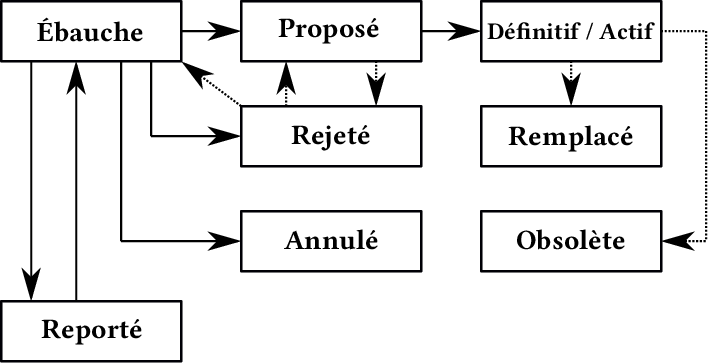
\includegraphics{chapters/img/bip-process-fr.png}

}

\caption{Diagram of the BIP adoption procedure, inspired by BIP-1.}

\end{figure}%

Note that these documents are used for BTC but also for other protocols.
For example, BIPs describing wallet functionalities (BIP-32, BIP-39,
BIP-44) are valid for the vast majority of cryptocurrencies. The SLIP-44
lists cryptocurrencies compatible with BIP-44. Other crypto-economic
protocols sometimes have their own proposal systems. Ethereum uses EIPs
(\emph{Ethereum Improvement Proposals}), Bitcoin Cash has CHIPs
(\emph{Cash Improvement Proposals}), Litecoin uses LIPs, and so on.

\section*{Verifying Consensus Rules}\label{verifying-consensus-rules}
\addcontentsline{toc}{section}{Verifying Consensus Rules}

\markright{Verifying Consensus Rules}

Bitcoin is based on a publicly accessible network of computers on the
Internet. This network follows a peer-to-peer model, where all network
members, called nodes, have equal privileges. These nodes ensure that
the consensus rules are respected. If a block is invalid (containing an
invalid transaction, for example), it is rejected by nodes enforcing the
rules.

In Bitcoin, nodes maintain a copy of the transaction ledger (the
blockchain) and, in doing so, ensure the validity of transactions and
blocks. They communicate with other network nodes and relay new
transactions and blocks, originating from users and miners,
respectively.

Consensus rule verification can be complete. In this case, the term
``full nodes'' emphasizes that they verify the entire chain. These nodes
download the entire blockchain, check the consensus rules, and relay
blocks and transactions. This is resource-intensive, both in terms of
data storage (as of November 2023, the Bitcoin chain was approximately
530 GB, and the entire UTXO set over 8.5 GB) and bandwidth (the average
size of blocks mined every 10 minutes was around 1.7 MB in November
2023).

Pruned nodes, which maintain the network state but not the entire chain,
are full nodes because they have verified compliance with the rules over
the entire chain. They simply cannot access the chain's history before a
certain date.

Verification can also be partial, in which case we speak of light
clients (or ``light nodes'' colloquially). This is useful for people who
have no interest in running a full node---for example, in hashing
software (implementing Stratum) and in lightweight wallets. They use a
method conceptualized in the Bitcoin white paper in 2008: Simplified
Payment Verification\footnote{Satoshi Nakamoto described Simplified
  Payment Verification as follows: ``It is possible to verify payments
  without running a full network node. A user only needs to keep a copy
  of the block headers of the longest proof-of-work chain, which he can
  get by querying network nodes until he is convinced he has the longest
  chain, and obtain the Merkle branch linking the transaction to the
  block it's timestamped in. He can't check the transaction himself, but
  by linking it to a place in the chain, he can see that a network node
  has accepted it, and blocks added after it further confirm the network
  has accepted it.'' --- Satoshi Nakamoto, \emph{Bitcoin: A Peer-to-Peer
  Electronic Cash System}, October 31, 2008.}.

Simplified Payment Verification (SPV) is a clever method that allows
novice and occasional users to interact easily with the protocol without
running a full node or blindly trusting a custodian. It significantly
reduces the load on lightweight wallets.

SPV relies on how transactions are chained and structured, as we saw in
Chapter \hyperref[ch:confirmation]{8}. First, the proof-of-work chain is
not strictly a chain of blocks but a chain of headers. This means light
clients only need to keep this chain of headers to determine the chain
with the most accumulated work. Since each header is 80 bytes, the
amount of data to store remains modest for modern devices: it increases
by about 4 MB per year, totaling just over 62 MB in November 2023.

Second, transactions are arranged in a Merkle tree, allowing light
clients to request only the branch information they're interested in to
verify the confirmation of one of their transactions. The number of
hashes to obtain and compute depends on the binary logarithm
(\(\log_{2}\)) of the number of transactions in the block. For a block
with 3,000 transactions (a high average on BTC), the load corresponds to
requesting 12 hashes of 32 bytes and performing 12 hash computations for
verification.

This simplified verification lightens the load on wallets but has major
drawbacks. First, it lacks reliability: nodes cannot lie by inventing a
transaction but can omit necessary information. This shortcoming can be
partially mitigated by increasing the diversity of network connections.
However, even then, verification remains vulnerable if the chain is
attacked by an entity controlling the majority of computing
power\footnote{This case was described by Satoshi Nakamoto in the white
  paper: ``As such, the verification is reliable as long as honest nodes
  control the network, but is more vulnerable if the network is
  overpowered by an attacker. While network nodes can verify
  transactions for themselves, the simplified method can be fooled by an
  attacker's fabricated transactions as long as the attacker can
  overpower the network. One strategy to protect against this would be
  to accept alerts from network nodes when they detect an invalid block,
  prompting the user's software to download the full block and alerted
  transactions to confirm the inconsistency. Businesses that receive
  frequent payments will probably still want to run their own nodes for
  more independent security and quicker verification.'' --- Satoshi
  Nakamoto, \emph{Bitcoin: A Peer-to-Peer Electronic Cash System},
  October 31, 2008.}.

Second, SPV lacks privacy because the client must reveal some of its
transactional activity through requests to network nodes. One way to
partially address this is to increase the amount of information
requested to mask essential details, but this method is far from
perfect\footnote{One initial way to address the privacy issue was to
  implement Bloom filters, as described in BIP-37, but this method was
  ineffective. See Arthur Gervais, Srdjan Capkun, Ghassan O. Karame,
  Damian Gruber, ``\emph{On the Privacy Provisions of Bloom Filters in
  Lightweight Bitcoin Clients}'', in \emph{Proceedings of the 30th
  Annual Computer Security Applications Conference}, December 2014,
  pp.~326--335: \url{https://eprint.iacr.org/2014/763.pdf}. There's also
  Neutrino, described in BIP-157 and BIP-158, which uses Golomb-Rice
  coding and requires more bandwidth.}.

Finally, SPV inherently provides partial verification. Not all consensus
rules are checked, meaning full nodes could agree on a rule change that
goes unnoticed by the light client. For example, SPV clients do not
verify constraints on block size, so the network could modify this limit
without their awareness. This explains the strategy of SegWit2X
proponents in 2017, who planned to double the block size limit without
replay protection so that SPV wallets would simply follow the longest
chain.

Satoshi believed the system could persist with centralized verification
by a few verifying nodes (including miners) and that other users would
employ light clients. In his first response to James A. Donald in
November 2008, he stated:

``Long before the network gets anywhere near as large as that, users can
use simplified payment verification (section 8) to check for
double-spending, which only requires having the chain of block headers
or about 12KB per day. Only people trying to create new coins would need
to run network nodes\footnote{Satoshi Nakamoto, \emph{Re: Bitcoin P2P
  e-cash paper}, 11/03/2008, 01:37:43 UTC:
  \url{https://www.metzdowd.com/pipermail/cryptography/2008-November/014815.html}.}.''

In this, he was mistaken. Verifying consensus rules needs to be
comprehensive for those rules to be enforced.

Thus, it is at the full node level that this verification occurs, a
reality sometimes encapsulated by the adage ``not your node, not your
rules\footnote{Understanding Bitcoin, \emph{Not Your Node Not Your
  Rules! w/ Ketominer, Udi Wertheimer, Francis Pouliot \& Mir Liponi}
  (video), April 5, 2019:
  \url{https://www.youtube.com/watch?v=jwaKVIEm-rI}.}.'' Don't trust,
verify! Much like a language results from the choices made by its
speakers, a computer protocol results from the rules enforced by full
nodes. This verification plays a crucial role in determining the
protocol.

\section*{Hard Forks}\label{hard-forks}
\addcontentsline{toc}{section}{Hard Forks}

\markright{Hard Forks}

Since Bitcoin is open and free, the consensus rules can be modified at
will by network nodes by changing the acceptance of blocks and
transactions. These modifications can lead to network conflicts and
potentially to a split into two separate networks, each managing its own
chain and currency. This phenomenon is referred to as a \emph{fork}.

Consensus rule changes are commonly categorized into two types:
\emph{hard forks}, which are brute and incompatible upgrades, and
\emph{soft forks}, which have a degree of backward compatibility. Let's
explore how these changes manifest, starting with hard forks before
describing soft forks.

In Bitcoin, the term \emph{fork} is polysemous, bearing four different
meanings: software fork, consensus rule fork, common chain fork, and
persistent chain fork. This polysemy can cause confusion, so different
terms are preferred for each meaning.

First, \emph{fork} is used in software development, particularly in free
software that permits and encourages this practice. It refers to
creating a program derived from the source code of an existing program
and, by extension, the derivative program itself. In this sense, the
reference implementation can undergo a fork, creating alternative
software. This software may adhere to the consensus rules (like Bitcoin
Knots) or deviate from them by creating a new protocol that shares the
chain's history (Bitcoin ABC, later Bitcoin Cash Node) or not
(Litecoin).

Second, \emph{fork} can denote the common branching of the blockchain,
by analogy with software development. The blockchain is not a linear
structure but a ``tree-shaped structure\footnote{Satoshi Nakamoto,
  source code of Bitcoin version 0.1:
  \url{https://github.com/trottier/original-bitcoin/blob/4184ab26345d19e87045ce7d9291e60e7d36e096/src/main.h\#L1001-L1008}.}''
that can have multiple branches of blocks, all compatible with the
consensus rules accepted by the network, with the correct branch
selected as the longest one (having the most accumulated work). This
type of branching occurs regularly in Bitcoin quite normally and
benignly when two miners simultaneously find different blocks, and it's
resolved when a new block is found.

Third, \emph{fork} can refer to a blockchain split caused by
incompatibility of consensus rules. This is called a hard fork or
``divergent fork.'' This split is usually permanent in the sense that
the two resulting branches cannot reconcile through Nakamoto's consensus
mechanism unless a very specific condition is met: if the majority
branch's rules form a restrictive subset of the minority branch's rules.
Ultimately, the two resulting chains are destined to exist on separate
networks.

Finally, \emph{fork} can, by metonymy, denote a change in consensus
rules, which can always cause a chain split and network separation. A
restriction of consensus rules is called a soft fork, or ``convergent
fork,'' due to its ability to result in a single branch. Any other
modification of consensus rules, whether an extension or strictly
incompatible change, is called a hard fork, referencing its propensity
to create a chain split. These are the two modifications we'll discuss
here\footnote{Note that the concepts are related. For example, a
  software fork (copy and modification) can implement a consensus rule
  fork (hard or soft fork) that ultimately creates a persistent chain
  fork (split).}.

The hard fork is the older concept compared to the soft fork. It was
previously termed an ``incompatible change\footnote{David François
  (davout), \emph{Re: Small protocol changes for flexibility},
  12/07/2010 15:08:02 UTC:
  \url{https://bitcointalk.org/index.php?topic=894.msg27757\#msg27757}.}.''
A hard fork is a non-restrictive modification of the consensus rules. It
causes a network conflict between nodes enforcing the old rules and
those enforcing the new ones.

A hard fork can be extensive, meaning it broadens the consensus rules on
blocks and transactions. Old nodes can thus produce valid blocks on the
new chain but not vice versa. A typical example of such a hard fork is
increasing the block size limit, accepting larger blocks---2 MB instead
of 1 MB, or 8 MWU instead of 4 MWU. This extensive hard fork is
illustrated in Figure \hyperref[fig:expanding-hard-fork]{10.1}.

\begin{figure}

{\centering 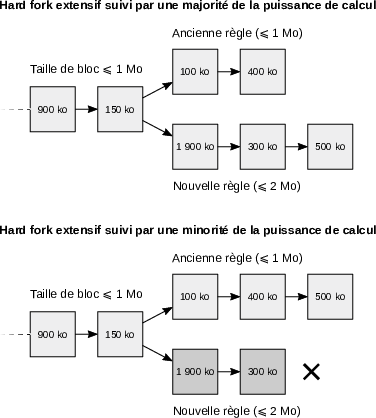
\includegraphics{chapters/img/expanding-hard-fork-induced-forks.png}

}

\caption{Diagram of an extensive hard fork: If the chain following the
new rule is longer than the one following the old rule, both chains
persist; otherwise, only the second survives.}

\end{figure}%

If the extensive hard fork is not supported by a majority of the
network's computing power, it may fail to create a persistent branch.
For instance, blocks from the branch imposing a smaller size limit are
entirely compatible with the new rules, so if it's longer, it will be
selected as the correct branch. To avoid this problematic situation,
hard forks are generally bilateral.

A bilateral hard fork is a hard fork that creates a total
incompatibility between the new rules and the old ones. This can involve
adding a rule requiring the first block of the fork to include an
incompatible change. In our block size limit increase example, this
would mean requiring the first block to be strictly larger than the
previous limit, as shown in Figure
\hyperref[fig:expanding-hard-fork-failure]{10.2}. This additional rule
is called wipeout protection.

\begin{figure}

{\centering 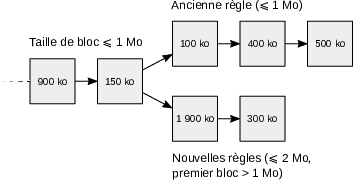
\includegraphics{chapters/img/bilateral-hard-fork-induced-fork.png}

}

\caption{Diagram of a bilateral hard fork: The new rules are strictly
incompatible with the old ones, so both chains persist.}

\end{figure}%

Another example is changing the transaction signature algorithm,
rendering all signed transactions and non-empty blocks strictly
incompatible. This change can also provide replay protection if two
competing chains persist.

Two scenarios can result from a hard fork: either the vast majority of
the economy adopts the change, resulting in a single chain, or the
economy fragments, and both chains persist. The first scenario is aimed
for in a planned upgrade hard fork, which doesn't intend to create two
separate chains. The second arises from a contentious hard fork due to
community division over the change. Accidental hard forks, caused by
unintended modifications of implicit consensus rules, are excluded
here\footnote{On March 11, 2013, the migration from version 0.7 to
  version 0.8 of the software implemented a shift from the Berkeley DB
  database system to LevelDB. However, it turned out that Berkeley DB
  had a default lock limit not present in LevelDB. Consequently, the
  migration constituted an accidental hard fork, causing a split from
  block 225,430 that lasted about 6 hours. The decision was ultimately
  made to revert to version 0.7, invalidating the 24-block branch mined
  on version 0.8's side, and to proceed with the migration months later.
  --- See Vitalik Buterin, ``\emph{Bitcoin Network Shaken by Blockchain
  Fork}'', \emph{Bitcoin Magazine}, March 13, 2013:
  \url{https://bitcoinmagazine.com/technical/bitcoin-network-shaken-by-blockchain-fork-1363144448};
  and Gavin Andresen, \emph{BIP-50: March 2013 Chain Fork Post-Mortem}:
  \url{https://github.com/bitcoin/bips/blob/master/bip-0050.mediawiki}.}.

A planned upgrade hard fork is a hard fork that requires synchronization
of almost the entire community. It usually results in a single chain,
effectively upgrading the protocol, though it's essentially economic
usage shifting from one protocol to another. It can be extensive, though
bilaterality is preferred for security reasons.

The first known planned upgrade hard fork was likely the addition of
\texttt{OP\_NOP} operation codes to version 0.3.6 of Bitcoin by Satoshi
Nakamoto in July 2010. Increasing block sizes was also considered a
planned upgrade hard fork, notably by Satoshi himself\footnote{In
  October 2010, following Jeff Garzik's proposal to increase the limit
  directly to 7.168 MB to ``match PayPal's average transaction rate,''
  Satoshi---well aware this was a ``network-incompatible'' fix---wrote:
  ``{[}The upgrade{]} can be introduced slowly, for instance: if
  (blocknumber \textgreater{} 115000) maxblocksize = largerlimit. It can
  start being introduced into versions long before then, so by the time
  it reaches the block number and takes effect, old versions that don't
  have it are already obsolete. When we get close to the limit block
  number, I can send out an alert to old versions so they know they need
  to upgrade.'' --- Satoshi Nakamoto, \emph{Re: {[}PATCH{]} increase
  block size limit}, 10/04/2010 19:48:40 UTC:
  \url{https://bitcointalk.org/index.php?topic=1347.msg15366\#msg15366}.},
until the contentious hard fork of Bitcoin Cash in 2017.

Outside of BTC, upgrades via hard fork are numerous, often due to a
smaller and/or more centralized economy. Examples include Bitcoin Cash,
Monero, Ethereum Classic, and Ethereum, where such upgrades occur
regularly.

A contentious hard fork aims deliberately to create a new chain,
stemming from a community disagreement so strong it leads to secession.
It's usually bilateral.

The first major example of a contentious hard fork was on Ethereum in
July 2016, following TheDAO hack. This hard fork sought to recover the
hacker's funds through an ``irregular state change.'' It was made
bilateral by a rule requiring the first 10 blocks post-activation to
include the string dao-hard-fork. Since the economic majority supported
the reversal, the altered chain retained the Ethereum name and ETH
ticker, while the other chain became Ethereum Classic with the ETC
ticker.

The second example is the hard fork that led to Bitcoin Cash's creation
in August 2017, following the scalability debate and the block size war.
This hard fork did not include SegWit, increased the block size limit to
8 MB, and improved the signature algorithm. It was made bilateral by a
rule requiring the activation block to be strictly larger than 1 MB. It
also effectively provided replay protection. Since this change happened
without the economic majority's agreement, the chain that didn't modify
the rules kept the Bitcoin name and BTC ticker, while the new chain
adopted the name Bitcoin Cash and the BCH ticker.

\begin{figure}

{\centering 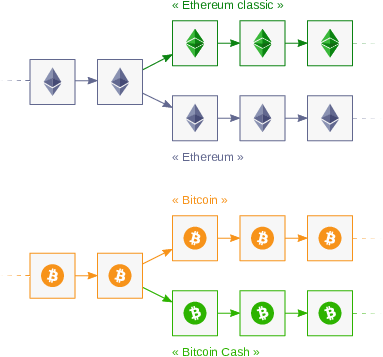
\includegraphics{chapters/img/hard-forks-eth-etc-bch-btc.png}

}

\caption{Examples of bilateral hard forks: ETH/ETC and BCH/BTC.}

\end{figure}%

Note that such a hard fork may involve modifying the difficulty
adjustment algorithm. If the computing power is too low to support it,
the adjustment might not occur in time. For this reason, Bitcoin Cash
implemented an Emergency Difficulty Adjustment (EDA) to adjust more
quickly. Ethereum Classic didn't need this, as Ethereum's adjustment
already occurred at every block.

\section*{Soft Forks}\label{soft-forks}
\addcontentsline{toc}{section}{Soft Forks}

\markright{Soft Forks}

Let's now discuss soft forks, a method of upgrade often misunderstood. A
soft fork is a restriction of the consensus rules. By essence, it
reduces the set of valid blocks and transactions by adding a rule or
modifying an existing one to be more restrictive. A typical example is
reducing the block size limit. The explicit addition of the 1 MB limit
in October 2010 was, therefore, a soft fork.

A soft fork can be applied while maintaining a single chain. If enforced
by the majority of the network's computing power, there's no risk of a
split. Blocks created by miners following the new rules are entirely
compatible with the old rules, so if the new rule chain is longer, it
will be considered the correct branch by all nodes. If the soft fork is
enforced by a minority, it results in two persistent chains. Both
scenarios are illustrated in Figure \hyperref[fig:soft-fork]{10.4}.

\begin{figure}

{\centering 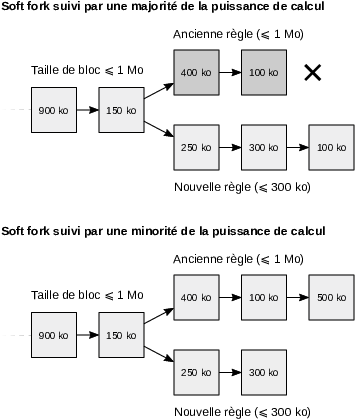
\includegraphics{chapters/img/soft-fork-induced-forks.png}

}

\caption{Diagram of a soft fork: If the chain following the new rule is
longer than the one following the old rule, only the first survives;
otherwise, both chains persist.}

\end{figure}%

The concept of a soft fork emerged after that of a hard fork. It was
formally discovered by Gavin Andresen in October 2011, who, following
his study of Nicolas van Saberhagen's proposal to add the
\texttt{OP\_EVAL} operation code\footnote{Nicolas van Saberhagen
  (ByteCoin), \emph{OP\_EVAL proposal}, 10/02/2011 00:49:19 UTC:
  \url{https://bitcointalk.org/index.php?topic=46538.msg553689\#msg553689}.},
realized that the upgrade could be done using the \texttt{OP\_NOP1}
operation code without necessarily causing a split\footnote{``I'm
  probably reading the code wrong, but I think OP\_EVAL wouldn't cause a
  blockchain fork!'' Gavin Andresen expressed on IRC. --- \#bitcoin-dev
  IRC logs, October 2, 2010, archived:
  \url{https://web.archive.org/web/20131201200245/http://bitcoinstats.com/irc/bitcoin-dev/logs/2011/10/02}.}.

The \texttt{OP\_NOP} operation codes are Bitcoin script instructions
added by Satoshi in July 2010 with the mere comment
``expansion\footnote{Satoshi Nakamoto, \emph{reverted makefile.unix
  wx-config -- version 0.3.6 (git commit)}, 07/29/2010 18:27:12 UTC:
  \url{https://sourceforge.net/p/bitcoin/code/119/}.}.'' The change
became effective with version 0.3.6 of the software, which also fixed
the 1 RETURN bug and was released on July 29. Their initial role is
silent: if they appear in a script, they do nothing but do not
invalidate the transaction. The direct consequence is that the behavior
of these operation codes can be modified without rendering scripts
incompatible with old consensus rules. The addition of this feature
indicates that Satoshi had grasped the soft fork mechanism.

A soft fork has a ``backward-compatible'' nature---or more accurately,
it's upward compatible, as compatibility is ascending, not
descending---in that old software versions can continue interacting with
the system. Non-mining nodes following old rules continue to see blocks
produced as valid. This characteristic is a major advantage over hard
forks.

However, this upward compatibility doesn't mean a soft fork is ``soft.''
It has a pernicious side in that it makes the modification hard to
grasp. Soft forks have several drawbacks.

First, they are not optional. If enforced by the majority of computing
power, a soft fork effectively resembles a censorship attack on users
following old rules. Thus, a soft fork has a coercive aspect that a hard
fork lacks.

Second, a soft fork is challenging to reverse. Newly added
functionalities cannot be simply deactivated; once adopted, there's no
easy rollback. Bitcoin SV developers, for instance, deactivated P2SH in
February 2020, exposing less attentive users to theft.

Third, a soft fork is not limited in scope. It can increase the
effective block size limit (via an auxiliary block, also called an
extension block or generalized soft fork). This extension block can also
include additional functionalities (like MimbleWimble in Litecoin). It
can even alter the protocol's monetary policy by redefining the base
unit\footnote{How a soft fork can introduce inflation into Bitcoin was
  explained by developer Peter Todd in 2016. --- Peter Todd,
  \emph{Forced Soft Forks}, January 18, 2016:
  \url{https://petertodd.org/2016/forced-soft-forks}.}.

Finally, a deep soft fork adds complexity due to the constraints of its
application. It introduces new exceptions to consensus rules, generating
technical debt for developers.

The archetype of a deep and complex soft fork was the SegWit upgrade, or
\emph{Segregated Witness}, which involved moving transaction signature
data (called \emph{witness} data) to a separate data structure to
eliminate transaction malleability. This upgrade, which occurred on
August 24, 2017, was initially supposed to be a hard fork until
developer Luke-Jr described in 2015 how to make it a soft fork. Backward
compatibility was ensured by linking the witness to the block via a
Merkle tree root placed in the coinbase transaction and by using
anyone-can-spend transaction outputs. Besides fixing the malleability
issue, it introduced a versioning system (allowing the later integration
of Schnorr-Taproot) and moderately increased the network's transaction
capacity, enabling effective block sizes to exceed 1 MB, up to 4 MB
theoretically. It also added four new address types to the protocol.

Moreover, a soft fork requires the majority of the network's computing
power to preserve its significance. If not followed by 51\% of computing
power in the medium term, its application results in a split. This
explains why miner activation is generally preferred over user
activation, even though the decision-making power ultimately lies with
the users, as we'll see in Chapter \hyperref[ch:determination]{11}.

On one hand, a User Activated Soft Fork (UASF) involves implementing the
soft fork in the software code to take effect at a specific block height
or timestamp. This method relies on the belief that the economy applying
the upgrade will be significantly majoritarian and that mining activity
will follow in the medium term due to higher block rewards.

On the other hand, a Miner Activated Soft Fork (MASF) makes activation
dependent on miners signaling support within validated blocks. It
activates when a certain signaling threshold (e.g., 95\%) is exceeded.
This method, whose procedure was described in BIP-9, ensures as much as
possible that miners apply the upgrade and that only one chain remains.

The same distinction exists in hard fork activation, but it holds little
relevance since computing power cannot prevent a split. Therefore, Miner
Activated Hard Forks (MAHF), long supported by proponents of increasing
the block size limit, have no particular advantage.

Like hard forks, soft forks can be categorized into two somewhat
distinct types: planned upgrade soft forks and contentious soft forks. A
soft fork is ideal for upgrading the protocol, allowing nodes to update
gradually. Although it requires some synchronization, it's not as
demanding as hard forks.

In BTC, soft forks have been favored by developers since their
discovery. Many upgrades have been soft forks, such as Pay to Script
Hash (BIP-16), the requirement to specify the block height in the
coinbase transaction (BIP-34), and the addition of a signature encoding
standard (BIP-66). The additions of \texttt{OP\_CHECKLOCKTIMEVERIFY} and
\texttt{OP\_CHECKSEQUENCEVERIFY} operation codes, allowing time locks in
the script language using \texttt{OP\_NOP2} and \texttt{OP\_NOP3}, were
also soft forks. More recently, the adoption of Schnorr-Taproot (or
simply Taproot) was a soft fork upgrade.

Litecoin also uses this type of transition. The protocol notably
integrated SegWit in May 2017 and Schnorr-Taproot and MimbleWimble
(MWEB) in May 2022.

A contentious soft fork aims to force a minority of the community to
follow the majority. If successful, there's only one chain; dissenters
have the choice to accept the rules or undertake a minority hard fork.
If it fails, two competing chains result.

SegWit is the typical example of a successful contentious soft fork. It
wasn't approved by all major actors (both large block proponents and
protocol purists like Mircea Popescu\footnote{Mircea Popescu,
  \emph{There's a one Bitcoin reward for the death of Pieter Wuille.
  Details below.}, December 10, 2015:
  \url{http://trilema.com/2015/theres-a-one-bitcoin-reward-for-the-death-of-pieter-wuille-details-below/}.}
opposed it), but it garnered majority support, allowing it to persist
and forcing dissatisfied ``big blockers'' to migrate to Bitcoin Cash.

An example of a failed contentious soft fork is Bitcoin ABC's team's
attempt to redirect 8\% of Bitcoin Cash's mining subsidy for their own
benefit on November 15, 2020\footnote{Amaury Séchet, \emph{Bitcoin ABC's
  plan for the November 2020 upgrade}, August 6, 2020:
  \url{https://amaurysechet.medium.com/bitcoin-abcs-plan-for-the-november-2020-upgrade-65fb84c4348f}.}.
This attempt, a soft fork due to its restrictive nature, led to a split
between a majority branch without redirection (BCH) and a minority
branch with it, later renamed ``eCash'' (XEC).

Thus, whether unanimously approved or only by a majority, soft forks are
superior to hard forks. Despite being sometimes more complex, they don't
require synchronization of the entire economy, allowing gradual
adaptation---a significant benefit for an open system used by a diverse
group like Bitcoin. Supermajority miner signaling minimizes the risk of
splits and preserves network effects as much as possible.

However, this major advantage comes at a cost: the clarity of consent.
In a hard fork, consent is clear---those who want the change are on the
chain they've chosen. In a soft fork, consent is more ambiguous---the
act of operating on the chain doesn't necessarily indicate active
acceptance of the change but perhaps passive resignation and a refusal
to undertake a minority hard fork. As Vitalik Buterin aptly wrote in
March 2017:

``Soft forks clearly favor coercion over secession systemically, whereas
hard forks have the opposite tendency\footnote{Vitalik Buterin,
  \emph{Hard Forks, Soft Forks, Defaults and Coercion}, March 14, 2017:
  \url{https://vitalik.ca/general/2017/03/14/forks_and_markets.html}.}.''

Therefore, even though they are generally superior, soft forks aren't
suitable for all situations.

\section*{Bitcoin's Plural Evolution}\label{bitcoins-plural-evolution}
\addcontentsline{toc}{section}{Bitcoin's Plural Evolution}

\markright{Bitcoin's Plural Evolution}

Bitcoin's open and free nature means its protocol can be modified at
will. Bitcoin evolves organically, slowly but surely; it's not a static
system with rules dictated by a central authority. Through this, it
improves over time.

This openness also implies that Bitcoin's implementation is necessarily
plural. Bitcoin is not a single system but an open model applied more or
less faithfully by several protocols. All implementations of Bitcoin
form a tree whose branches come from the same trunk and roots.

However, not all branches are equal; not all implementations are equally
important. One of them (BTC) is now supermajoritarian, so we naturally
call it Bitcoin, and modifying it is (fortunately) difficult. In the
next chapter, we'll examine the underlying mechanism that makes Bitcoin
what it is today and how protocol evolution is governed.

\begin{figure}

{\centering 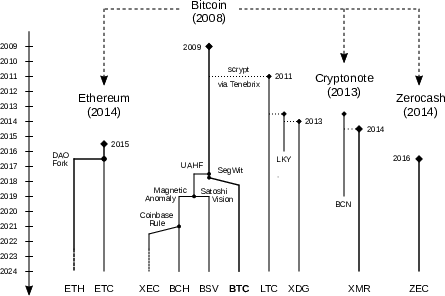
\includegraphics{chapters/img/bitcoin-forks-tree.png}

}

\caption{Conceptual variations, software modifications, and consensus
forks of Bitcoin.}

\end{figure}%

\bookmarksetup{startatroot}

\chapter{Determining the Protocol}\label{ch:determination}

\phantomsection\label{enotezch:11}{}

\textbf{{I}\textsc{n}} Bitcoin, the protocol comprises the open set of
rules involved in the creation and transmission of blocks and
transactions across the network. Notably, it includes the consensus
rules that govern the validity of the ledger upon which network nodes
agree. These rules are implemented through software applications that
can be freely copied, modified, and reused at will.

This open and free nature means there is no central authority decreeing
the rules, as is common in centralized models; instead, decision-making
is distributed within the community. Therefore, determining the protocol
is not a technical mechanism but an economic one, aligning with
Bitcoin's fundamentally monetary nature.

This topic is of paramount importance because this mechanism ensures the
integrity of the consensus rules and, consequently, the proper
functioning of the system. In particular, it underpins the renowned
resistance to inflation---the difficulty of creating more bitcoins.
Therefore, it is crucial to have a solid understanding of this mechanism
if we are to be convinced of Bitcoin's viability.

\section*{Resistance to Inflation}\label{resistance-to-inflation}
\addcontentsline{toc}{section}{Resistance to Inflation}

\markright{Resistance to Inflation}

One of Bitcoin's two major promises is to resist monetary
inflation---that is, to make it difficult to create additional units
beyond what the market accepts. This promise is substantial: as we saw
in Chapter~\hyperref[ch:adversaire]{4}, the state does everything in its
power to benefit from monetary creation, a phenomenon known as
seigniorage. At first glance, it seems surprising that a digital entity
could possess such a property.

Bitcoin's original monetary policy was established by Satoshi Nakamoto
when the prototype was launched on January 8, 2009. This policy was
straightforward: monetary creation would be halved every four years,
becoming negligible over time. The plan was to create 10.5 million units
linearly over the first four years, 5.25 million over the next four,
2.625 million over the following four, and so on, limiting the total
number of units in circulation to 21 million. Bitcoin was envisioned to
become a currency with a fixed supply---something unprecedented in
history.

This monetary policy became one of Bitcoin's selling points, leading
some to believe it was immutable and carved in stone, with the
mathematical application of Satoshi Nakamoto's decree guaranteeing the
system's resistance to inflation. For instance, Tyler Winklevoss, who
invested in bitcoin with his twin brother Cameron, was convinced in 2013
that he had purchased an asset free from human intervention:

``We have elected to put our money and faith in a mathematical framework
that is free of politics and human error\footnote{Nathaniel Popper,
  Peter Lattman, ``\emph{As Big Investors Emerge, Bitcoin Gets Ready for
  its Close-Up}'', \emph{CNBC}, April 11, 2013:
  \url{https://www.cnbc.com/id/100635418}.}.''

However, this belief is, at best, a misguided approximation. It's not
sufficient for a rule to have been decreed in the past for it to
manifest in present reality; it also requires acceptance and application
by others. This acceptance is inherently subject to politics and human
error.

Confusion exists regarding bitcoin's fixed monetary policy. Notably,
Satoshi Nakamoto never specified how it could be safeguarded. Various
theories have been proposed, ranging from miner intervention to the need
for community unanimity, or even attributing legal authority to
Satoshi's decree. In all cases, the discussion revolves around
``governance\footnote{Pierre Rochard, \emph{Bitcoin Governance}, July 9,
  2018:
  \url{https://pierre-rochard.medium.com/bitcoin-governance-37e86299470f}.}''
or ``social consensus\footnote{Arthur Breitman mentioned \emph{social
  consensus} as early as August 2014 in the first formal description of
  Tezos.---Arthur Breitman, \emph{Tezos: A Self-Amending Crypto-Ledger},
  August 3, 2014: \url{https://tezos.com/position-paper.pdf}.}''---that
is, how Bitcoin's rules are decided. This is the issue we refer to as
determining the protocol.

\section*{The Influence of Merchants on the
Protocol}\label{the-influence-of-merchants-on-the-protocol}
\addcontentsline{toc}{section}{The Influence of Merchants on the
Protocol}

\markright{The Influence of Merchants on the Protocol}

As we've suggested, the protocol is determined by economic forces. Since
Bitcoin is an economic system, it's natural that its governing rules
emerge from the market rather than from a fixed past decree or a current
central authority.

The notion that the economy shapes the rules isn't new. As early as
spring 2012, Meni Rosenfeld wrote on Stack Overflow that changing the
protocol required ``an economic majority, i.e., adoption by the users
and businesses that give the currency value\footnote{Meni Rosenfeld,
  \emph{Re: How could the bitcoin protocol be changed? Has this ever
  occurred?}, June 14, 2012, 13:53:19 UTC:
  \url{https://bitcoin.stackexchange.com/questions/3945/how-could-the-bitcoin-protocol-be-changed-has-this-ever-occurred\#comment4983_3948}.}.''
Gavin Andresen echoed this idea in May 2015 when discussing increasing
the block size limit:

``If we can't reach consensus here, the ultimate authority for
determining consensus is the code used by the majority of merchants,
exchanges, and miners\footnote{Gavin Andresen,
  \emph{{[}Bitcoin-development{]} Proposed alternatives to the 20MB step
  function}, May 29, 2015, 12:39:30 UTC:
  \url{https://lists.linuxfoundation.org/pipermail/bitcoin-dev/2015-May/008340.html}.}.''

However, the clarity of this concept only emerged after the events of
the blocksize war, during which the underlying mechanisms became
apparent. It wasn't developers or miners deciding the rules but rather
the users, and more precisely, the \emph{merchants}. Eric Voskuil wrote
in November 2018:

``Bitcoin does not rely on a custodian, but for the sake of establishing
a general principle, one can consider the set of all merchants as the
collective custodian of Bitcoin\footnote{Eric Voskuil, ``Custodial Risk
  Principle,'' in \emph{Cryptoeconomics: Fundamental Principles of
  Bitcoin}, Amazon KDP, 2022, pp.~34--35.}.''

Merchants, broadly defined, are those who provide goods, services, or
other currencies in exchange for bitcoin at market-acceptable prices.
This activity is evident through actual transactions with customers and
can be measured by the revenue received. In this way, merchants
contribute to bitcoin's utility, gauged by the quantity of goods and
services it facilitates acquiring, and thus to the economic significance
of the chain\footnote{This was recognized in January 2010 by
  NewLibertyStandard, Bitcoin's first merchant, who stated: ``Everyone
  who buys or sells goods using bitcoins, including exchangers, advances
  the Bitcoin economy.''---NewLibertyStandard, \emph{Re: New Exchange
  Service: ``BTC 2 PSC''}, January 19, 2010, 08:06:15 UTC:
  \url{https://bitcointalk.org/index.php?topic=15.msg111\#msg111}.}. By
operating nodes that verify consensus rules, they participate in
determining the protocol in proportion to their potential economic
activity.

Referring to a single, changeable protocol is inaccurate: as sets of
rules, protocols are each fixed, but their use and utility vary.
Modifying the protocol involves creating a new protocol whose resulting
chain becomes economically more significant than any competing branches,
including the one adhering to the original protocol\footnote{Jeff Garzik
  aptly noted in October 2010 that ``the effort to increase the
  transaction rate limit {[}was{]} the same as changing the fundamental
  nature of bitcoins: convincing the vast majority to upgrade.''---Jeff
  Garzik, \emph{Re: {[}PATCH{]} increase block size limit}, October 4,
  2010, 18:33:55 UTC:
  \url{https://bitcointalk.org/index.php?topic=1347.msg15342\#msg15342}.}.
For example, SegWit was a contentious soft fork, but the resulting
protocol was far more valued than competing protocols (BTC pre-SegWit
and Bitcoin Cash), so we can say the BTC protocol was upgraded through
this modification.

Bitcoin, as a concept, naturally encompasses multiple protocols due to
its open and free nature. There's not just one Bitcoin protocol but
several, much like there are multiple Linux distributions or various
forms of the dollar. These protocols compete to gain utility through
merchant adoption.

What truly matters is the economic weight of the chains these protocols
create. Anyone can define Bitcoin as they wish, perhaps declaring
there's only one protocol that cannot be altered without unanimity, but
this stance doesn't change the economic realities. If a modified chain
captures 80\% of economic activity, the chain following the original
protocol rules would continue to exist but would be significantly
downgraded and lose relevance. As Arthur Breitman noted in 2014, ``the
option of sticking with the original protocol is not at all relevant if
the value of its tokens is annihilated by a change in
consensus\footnote{Arthur Breitman, \emph{Tezos: A Self-Amending
  Crypto-Ledger}, August 3, 2014:
  \url{https://tezos.com/position-paper.pdf}.}.''

This explains the practices that have naturally evolved within the
ecosystem. We typically refer to Bitcoin as the main and economically
dominant implementation of the concept. In cases of a split, the name
and market ticker of the original protocol are usually retained by the
majority branch, whether it keeps the initial rules (Bitcoin-BTC) or
modifies them (Ethereum-ETH). The minority branch must then adjust its
name, either by extending it to emphasize continuity (Bitcoin Cash,
Bitcoin SV, Ethereum Classic) or by adopting a new brand (e.g.,
``eCash''~/XEC).

This economic mechanism means resistance to change comes from merchants
who refuse to adopt new rules. Therefore, a modification that would
undermine Bitcoin's fundamental properties---such as introducing
censorship or inflation---would only take effect if merchants accepted
it. Merchants benefit from these fundamental properties through the
freedom offered by the absence of censorship (facilitating, for example,
tax evasion) and the increasing purchasing power of the funds received,
incentivizing them to reject such changes. Specifically, bitcoin's
``natural deflation\footnote{Satoshi Nakamoto, \emph{Re: A few
  suggestions}, December 13, 2009, 16:51:25 UTC:
  \url{https://bitcointalk.org/index.php?topic=12.msg62\#msg62}.}''
serves as the economic incentive maintaining its unique monetary policy.

Similar to mining security, the commercial security of a chain---that
is, the difficulty of altering its fundamental properties---doesn't
depend solely on its economic activity (revenues). It also hinges on the
distribution of this activity and the number of merchants relative to
the global population\footnote{Eric Voskuil, ``Qualitative Security
  Model,'' in \emph{Cryptoeconomics: Fundamental Principles of Bitcoin},
  Amazon KDP, 2022, pp.~59--62.}. If economic activity is concentrated
in the hands of a single actor, modifying the protocol becomes easy.
Likewise, if high economic activity is evenly distributed among a small
number of merchants, the protocol is more susceptible to change than if
a large number of merchants are involved.

Just as miners may delegate their transaction selection power
(``hashers''), merchants can delegate their power to verify consensus
rules. Merchants relinquish this power to custodial services, paying a
commission to reduce usage complexity (such as node deployment) and
transaction costs (through fee discounts). These custodial services
might include wallet providers (Electrum, Acinq, Edge, Ledger, Trezor),
payment processors (BitPay, Coinbase Commerce), or even block explorers
(Blockchair, Mempool.space).

Delegating verification poses an obvious centralization issue. While the
economy can adapt and return to health in the medium term through new
node deployments, the immediate commercial security of the chain
suffers. An attack aiming to modify or eliminate the protocol can
inflict significant short-term damage.

This impact intensifies if delegation involves asset custody with a
third party, effectively making the custodian the real merchant with
full control over the funds. This scenario is common with online
exchanges that buy and sell other currencies using bitcoin while
maintaining internal order books to balance supply and demand.

As of this writing, Bitcoin's situation is unique because economic
activity is dominated by exchanges between bitcoin and official
currencies. Even during Satoshi's time, exchangers were Bitcoin's first
merchants: the inaugural purchase using bitcoin wasn't a pizza, as often
recounted, but \$5.02 via PayPal\footnote{On October 12, 2009, the first
  merchant, NewLibertyStandard, ``sold'' \$5.02 for 5,050 BTC to Martti
  Malmi, the first customer. One could argue that the miner of block
  2,817, who received 2 BTC in transaction fees on February 3, 2009, was
  technically the first merchant for his service, but the amount was
  negligible.}. Today, centralized exchanges like Kraken, Coinbase, and
Binance have taken the lead, resulting in an economy that's highly
centralized and vulnerable to attacks.

As with censorship attacks, efforts to alter Bitcoin's fundamental
properties are unlikely to originate from rational economic actors, who
have no incentive to do so, but rather from political agents acting on
behalf of the state. Such an attack would align with state objectives
like combating money laundering and terrorist financing (AML/CFT) or
curbing speculation against the national currency. Highly regulated
exchanges would be the primary targets.

Thus, merchants determine the protocol by choosing consensus rules that
suit them, which they consistently verify using their nodes. A
merchant's individual power is weighted by their potential economic
offerings, estimated by actual economic activity. However, this power
isn't linear, as it significantly depends on the network effect.

\section*{The Network Effect}\label{the-network-effect}
\addcontentsline{toc}{section}{The Network Effect}

\markright{The Network Effect}

A merchant's direct power isn't solely individual. Since Bitcoin is a
currency, it's subject to economic phenomena, the most significant being
the network effect. This effect explains why there are fewer viable
Bitcoin implementations than one might expect for a typical physical
product.

The network effect refers to the phenomenon where the actual utility of
a technology or product increases with the number of its users. It's a
self-reinforcing cycle---a virtuous circle: the more users a system has,
the more it attracts new users.

Currency functions as a social network and is thus subject to the
network effect. The overall utility of the network doesn't grow linearly
with its economic size but super-linearly. This concept is expressed by
Metcalfe's Law, which states that ``the utility of a network is
proportional to the square of the number of its users\footnote{Metcalfe's
  Law is named after Robert Metcalfe, co-creator of the Ethernet
  protocol and founder of 3Com, who observed this effect in 1980
  regarding compatible communication devices. The law was formally
  stated by George Gilder in 1993 in an article in \emph{Forbes},
  suggesting network utility scales as \(n^2\) with \(n\) users, which
  overestimated the actual network effect. In 2006, Odlyzko's Law
  proposed a more conservative utility scaling of \(n \log n\).---George
  Gilder, \emph{Metcalf's Law and Legacy}, September 1, 1993:
  \url{https://www.discovery.org/a/41/}; Bob Briscoe, Andrew Odlyzko,
  Benjamin Tilly, \emph{Metcalfe's Law is Wrong}, July 1, 2006:
  \url{https://spectrum.ieee.org/metcalfes-law-is-wrong}.}.''

During the rise of the internet, the demand for a common protocol led
TCP/IP to prevail over the competing OSI model of the time. Similarly,
only a limited number of languages tend to dominate due to communication
constraints. In international trade and diplomacy, there's generally
only one lingua franca within a given region. Historically, this has
included Aramaic and Koine Greek in the Near East during Antiquity,
Italian in Europe at the start of the Renaissance, French as the
diplomatic language in the 18th and 19th centuries, and today, English
globally.

For currencies, the network effect arises from individuals' preference
for a single currency. This is internally driven by the mental cost of
economic calculations involving multiple currencies and externally by
the exchange costs incurred when converting one currency to another.
Consequently, people tend to favor using the most popular currency, even
if it has flaws. Additionally, a currency used by a small group must
offer significant advantages over others to endure. Over time,
currencies tend to consolidate into a single dominant form, though
barriers to complete unification may persist.

In Bitcoin, the monetary network effect is predominant. While it's not
the only network effect, it's the one that drives others---such as
liquidity, software development, economic security, and marketing
communication---to manifest\footnote{Vitalik Buterin, \emph{On Bitcoin
  Maximalism, and Currency and Platform Network Effects}, November 19,
  2014:
  \url{https://blog.ethereum.org/2014/11/20/bitcoin-maximalism-currency-platform-network-effects}.}.

Therefore, the network effect plays a \emph{crucial} role in determining
the protocol. The existence of a limited number of viable Bitcoin
implementations and their stability results from this effect. This is
why an economic supermajority is often sought before implementing
protocol changes. It also encourages the ossification of the protocol in
response to numerous change proposals. A natural Schelling point opposes
altering consensus rules\footnote{A Schelling point, in game theory, is
  a solution that players in a coordination game tend to adopt in the
  absence of communication, because it seems natural or
  prominent.---Thomas C. Schelling, \emph{The Strategy of Conflict},
  Harvard University Press, 1960.}: in the absence of a clear intent to
modify the rules or in case of dispute, the default option is to do
nothing.

The network effect explains the tendency toward maximalism within
communities associated with specific protocols and units of account.
Since there should logically be only one Bitcoin, any attempt to alter
the concept is seen as futile and counterproductive, if not fraudulent.
However, maximalism overlooks the substitution effect.

\section*{The Substitution Effect}\label{the-substitution-effect}
\addcontentsline{toc}{section}{The Substitution Effect}

\markright{The Substitution Effect}

The second key economic influence on merchants' individual power is the
substitution effect. This effect directly opposes the network effect and
leads to a greater number of Bitcoin implementations than one might
expect if the concept weren't naturally constrained.

In economics, a substitute product is a good or service that can be used
for the same purpose as another but has different characteristics.
Consumers may choose a substitute because it's cheaper or more effective
in meeting their needs. Examples abound: wheat or rice for
carbohydrates, coffee or tea for caffeine intake, trains or planes for
public transportation, and so on. Substitution is typically imperfect
since the alternative product will have differences that can't be
quantified.

The substitution effect emerges when market conditions change
dramatically. The original product might become more expensive or
scarce, or perhaps cheaper or more abundant. Shifts in living standards
may also lead consumers to prefer one product over another. In all
cases, a significant change triggers substitution.

This effect also applies to currencies. It becomes evident when official
currencies collapse, such as in hyperinflation scenarios, or when they
are banned, like in prisons. In these situations, non-traditional items
like cars or cigarettes may become monetized.

With Bitcoin, the substitution effect manifests uniquely. Each
implementation of Bitcoin is limited by a transaction capacity ceiling,
often defined by a maximum block size or weight\footnote{Implementing
  layer-2 solutions like the Lightning Network only enhances effective
  value transfer capacity, as we'll discuss in
  Chapter~\hyperref[ch:scalabilite]{14}.}. Additionally, the total
number of bitcoins is capped. When demand for monetary activity
increases, instead of creating more bitcoins, the cost of including
transactions in a block rises.

This characteristic economically excludes transactions involving amounts
too small to justify the cost of recording them on the chain. However,
the demand for these small transfers doesn't vanish. Consequently, some
of this demand shifts to alternative chains with lower fees, such as
Litecoin or Bitcoin Cash, which offer less security than BTC\footnote{This
  shift to cheaper related systems was observed by Matt Ahlborg, market
  research consultant for Bitrefill, a platform selling phone top-ups
  and gift cards.---Matt Ahlborg on Twitter, April 17, 2023, 14:14 UTC:
  \url{https://twitter.com/MattAhlborg/status/1647966711126147072}.}.

Similarly, what is often perceived as a lack of functionality in
Bitcoin-BTC is actually a matter of cost. While it's possible to
simulate all functionalities present on other chains in innovative and
indirect ways, it's cheaper and easier to use protocols that natively
incorporate them. This is the case with Monero for privacy or
Ethereum-ETH and Ethereum Classic for general programmability.

Therefore, the substitution effect plays a significant role in Bitcoin
and crypto-economic systems in general, explaining the existence of
numerous ``alternative cryptocurrencies.'' Without this effect, economic
activity might have naturally consolidated around a single protocol
(BTC), but we see that's not the case, especially during network
congestion.

The substitution effect accounts for the trend toward extreme
crypto-monetary pluralism, where advocates claim that any slightly
superior technology could dethrone the market-leading protocol. In this
view, they heavily underestimate the network effect, making the opposite
mistake of maximalists.

\section*{Power and Influence}\label{power-and-influence}
\addcontentsline{toc}{section}{Power and Influence}

\markright{Power and Influence}

To more precisely understand how the protocol evolves, we should
distinguish between \emph{power} and \emph{influence} within Bitcoin. In
politics, power is the ability to act without third-party consent,
ultimately enforced through physical means. Influence, by contrast, is
the capacity to sway the decisions of those who hold power, often
wielded by religious or ideological forces.

In Bitcoin, power translates to the economic authority merchants have
over the protocol. Through their nodes, they verify the consensus rules
associated with the unit of currency they accept in commerce, thereby
adding economic utility to it. However, this direct economic power is
frequently influenced by various actors.

These influences are considered in the traditional governance model of
Bitcoin, which typically involves the trio of developers, miners, and
users. These internal system participants engage more or less directly.

Moreover, influence over the protocol also comes from external entities
that impact the system diffusely. While it's impossible to list all
external influences exhaustively, we can identify key ones. These
influences operate in three primary ways---through discourse, money, and
force---and relate to three actor categories: opinion leaders, financial
powers, and state authorities.

Thus, merchants face a range of influences from internal participants
like developers, miners, and other users, as well as from external
actors such as ideological influencers, financiers, and regulators.
These groups interact with each other, forming a complex sociological
network that influences the final protocol choice. While fully
explaining this complex interplay is beyond our scope, we can sketch a
general model by examining internal pressures before exploring the more
diffuse external forces.

\begin{figure}[H]

{\centering 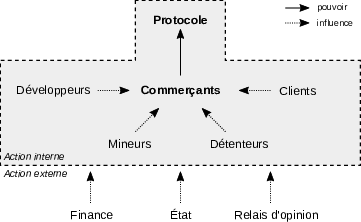
\includegraphics{chapters/img/bitcoin-governance-model.png}

}

\caption{A Bitcoin governance model: interactions of the main actor
groups in determining the protocol.}

\end{figure}%

\section*{The Influence of
Developers}\label{the-influence-of-developers}
\addcontentsline{toc}{section}{The Influence of Developers}

\markright{The Influence of Developers}

Developers constitute the first category of internal actors. They work
directly on maintaining and upgrading full or partial implementations of
the protocol, contributing to the chain's health through the software
used by merchants and miners. The reference implementation---the most
widely used and the model for other implementations---is particularly
significant.

This intermediary role grants developers considerable influence over
merchants and other actors who often lack the expertise to analyze and
understand the code directly. Additionally, maintaining high-performance
software requires costly effort, not easily replicated. This positions
developers strongly in protocol decision-making.

Developers are diverse, with varying opinions. To address this, they
often rely on the concept of \emph{rough consensus}, which isn't strict
consensus but rather an estimation of group sentiment or general will.
Utilizing rough consensus practically achieves near unanimity without
allowing individual dissent to disrupt the process\footnote{The concept
  of \emph{rough consensus} was used by the Internet Engineering Task
  Force (IETF) in 1998, described in their working group procedures:
  ``Working groups make decisions through a `rough consensus' process.
  IETF consensus does not require that all participants agree, but
  rather that a general sense of agreement is achieved.''---\emph{IETF
  Working Group Guidelines and Procedures}, September 1998:
  \url{https://datatracker.ietf.org/doc/html/rfc2418}.}. While excluding
dissenting voices can be critiqued (since an individual might be correct
against the majority), it helps preserve the protocol's network effect
by presenting a unified proposal to merchants.

For BTC, Bitcoin Core serves as the reference implementation, overseen
by maintainers. These maintainers, and developers more broadly, are
viewed as the protocol's guardians. While it's possible to use an
alternative implementation (a ``fork''), doing so is costly and often
frowned upon, creating inertia favoring Bitcoin Core.

This dominance has historically led to the rejection of several
dissenting efforts, occasionally resulting in alternative
implementations:

\begin{itemize}
\item
  In 2014, Mike Hearn sought to add a \texttt{getutxos} network request
  to Bitcoin Core but was denied due to lack of consensus, leading to
  the creation of Bitcoin XT.
\item
  Proponents of increasing the network's transaction capacity during the
  blocksize war launched multiple implementations in attempts to enact
  change: Bitcoin XT in mid-2015, Bitcoin Classic in early 2016, Bitcoin
  Unlimited in mid-2016, and btc1 in mid-2017.
\item
  Opponents of the SegWit upgrade, widely supported by Bitcoin Core, had
  to develop Bitcoin ABC, which also increased the block size limit,
  resulting in the creation of Bitcoin Cash.
\item
  In 2022, Jeremy Rubin threatened to activate BIP-119 (a soft fork)
  through miners due to Bitcoin Core's refusal to integrate his code
  change but eventually reconsidered, likely after gaining the desired
  attention.
\end{itemize}

Thus, while developers---especially those with Bitcoin Core---wield
significant influence over the protocol, this influence is limited. If
they oppose economic interests too starkly, they risk being replaced by
other developers.

A notable example of successful dissent is found in Monero's early
history\footnote{dEBRUYNE, \emph{Re: Monero inception---how did
  bitmonero become monero?}, August 11, 2016, 16:21:
  \url{https://monero.stackexchange.com/questions/1011/monero-inception-how-did-bitmonero-become-monero/1024\#1024}.}.
Monero originated as Bitmonero in April 2014, launched by a developer
known as thankful\_for\_today to revive the Bytecoin project, which had
experienced massive premining. However, thankful\_for\_today,
self-designated as a ``benevolent dictator,'' made unilateral changes
without consultation, leading to his ousting after a few days. A team of
six developers then forked the project, renaming it Monero.

Another example is the opposition to Bitcoin ABC within the Bitcoin Cash
protocol in 2020. Bitcoin ABC, the reference implementation for Bitcoin
Cash since 2017, was led by Amaury Séchet. In 2020, he agreed with
miners' suggestions to implement a soft fork redirecting part of the
block reward to development teams and integrated this change into
Bitcoin ABC in November. An alternative implementation, Bitcoin Cash
Node, was created to counter this change, gathering substantial economic
support and becoming the reference implementation for what is still
called Bitcoin Cash today. Implementing the protocol's subsidy
redirection led to the creation of the XEC protocol.

Therefore, while developers have real influence over the protocol, it's
fundamentally limited by economic forces when they come into play.

\section*{The Pressure from Miners}\label{the-pressure-from-miners}
\addcontentsline{toc}{section}{The Pressure from Miners}

\markright{The Pressure from Miners}

Miners represent the second category of actors influencing the protocol.
They are individuals or groups who confirm transactions by expending
energy through proof of work. As discussed in
Chapter~\hyperref[ch:censure]{9}, miners have the power to select
transactions, enabling them, if they hold a majority, to perform
double-spending or enforce censorship.

Contrary to some beliefs, miners have direct power over the protocol
only insofar as they are a specific type of merchant. They participate
in the economy by confirming transactions in exchange for fees. However,
their direct power is minimal due to their relatively small economic
activity compared to the total.

Nonetheless, miners wield significant influence in decision-making
because of their potential to attack the consensus. They can, for
instance, influence economic choices during a split by attacking
competing branches to undermine them. This was threatened by pro-BSV
miners in November 2018 following the separation from BCH\footnote{A
  ``hash war'' occurred between Bitcoin SV miners, supported by Craig
  Wright and Calvin Ayre, and Bitcoin ABC miners, backed by Roger Ver
  and Jihan Wu, involving the redirection of mining power.---Aaron van
  Wirdum, \emph{Week 2: How the Bitcoin Cash `Hash War' Came and Went
  and Not Much Happened}, November 30, 2018:
  \url{https://bitcoinmagazine.com/technical/week-2-how-bitcoin-cash-hash-war-came-and-went-and-not-much-happened}.}.
Similarly, pro-BCHN miners censored the Bitcoin ABC chain in November
2020.

Miners can also influence economic choices by imposing a soft fork that,
in practice, is indistinguishable from censorship. The original
consensus rules remain, but their full expression is hindered,
potentially prompting merchants to adopt the soft fork by refusing
non-conforming transactions and blocks. Developer Peter Todd described
this as a ``forced soft fork\footnote{Peter Todd, \emph{Forced Soft
  Forks}, January 18, 2016:
  \url{https://petertodd.org/2016/forced-soft-forks}.},'' sometimes
referred to as an ``evil fork.'' The situation can resolve in two ways:
merchants might continue applying the old rules, creating a fee
differential incentivizing miners to revert, or they may adopt a hard
fork to counter the soft fork, risking a spiral of splits due to rapid
human intervention.

However, miners' influence ends there. Merchants ultimately determine
the rules, and miners are powerless against this reality. It's incorrect
to assert that miners control the protocol (governance by proof of
work), as some ``big blockers'' did during the blocksize war\footnote{This
  viewpoint was held by Coinbase CEO Brian Armstrong, who wrote on
  January 3, 2016: ``Fortunately, Bitcoin has an elegant built-in
  upgrade mechanism. If the majority of Bitcoin miners `vote' for a
  particular upgrade, it is by definition the new version of
  Bitcoin.''---Brian Armstrong, \emph{Scaling Bitcoin: The Great Block
  Size Debate}, January 3, 2016:
  \url{https://www.coinbase.com/blog/scaling-bitcoin-the-great-block-size-debate}.}.
If that were true, Bitcoin's economic system would be doomed, since
miners would be naturally incentivized to increase their revenue through
inflation, much like central banks.

\section*{The Role of Users}\label{the-role-of-users}
\addcontentsline{toc}{section}{The Role of Users}

\markright{The Role of Users}

Non-merchant users form the third category of internal actors
influencing the protocol. Users are often highlighted as having the
final say over the protocol\footnote{``The Bitcoin network isn't
  controlled by anyone, much like no one owns the technology behind
  email. Bitcoin is controlled by all its users globally. While
  developers improve the software, they can't force changes to the
  Bitcoin protocol because users are free to choose which software and
  version they use. To remain compatible, users need to use software
  adhering to the same rules. Bitcoin can only function correctly with
  complete user consensus.''---Bitcoin.org FAQ:
  \url{https://bitcoin.org/en/faq\#who-controls-the-bitcoin-network}.}.
However, the term ``user'' is ambiguous and can be misleading because
using bitcoin generally involves three distinct actions: accepting it in
commerce, holding it over time, and spending it with others. This leads
to three theoretical subcategories: merchants, customers, and holders.
Only the first has effective power over the protocol; the others wield
influence.

First, consider customers---those exchanging their bitcoins for goods
and services, including other currencies. They are the counterpart to
merchants; trade is inherently reciprocal: without buyers, there are no
sellers, and vice versa. Thus, merchants and customers are
interdependent.

Customers exert significant influence in determining the protocol. A
merchant aiming for business success must accept at least the currency
linked to the protocol favored by the majority of customers. The
rejection of SegWit2X in 2017 exemplifies customer influence, where
users swayed major merchants (exchanges) to abandon plans to double the
block size limit in November.

However, the notion that customers share control of the protocol with
merchants is flawed. If user dissent is evenly split, the merchant
decides which protocol to adopt to offer goods and services at
acceptable prices. Ultimately, customers (who spend their bitcoins)
don't add utility to the currency; merchants do.

Next are holders---those who keep bitcoins over extended periods.
Referred to as savers or HODLers (a play on the word ``hold''), they
emphasize their intent to retain their bitcoins long-term. By doing so,
they restrict the money supply, which, coupled with increased demand,
elevates the purchasing power of each unit and its exchange rate with
the dollar---commonly known as ``the price.''

Holders influence merchants in several ways. First, their savings
increase the size of the protocol's subsidy, boosting the mining budget
for protection against double-spending, thus providing greater security
for merchants. Second, holding offers the market more potential
liquidity, enabling larger participants to enter. Third, a higher price
generates significant publicity, attracting media attention through
speculative interest. Thus, during a chain split, holders can sell one
branch's currency for another, creating a differential favoring the
preferred protocol (as seen in the BTC and BCH split).

Believing that the currency's purchasing power is paramount has led some
crypto-economic protocols, like Dash and Tezos, to innovate with
internal governance systems resolving protocol disputes through votes
proportional to unit ownership (governance by proof of stake). Holders
are akin to stakeholders in a company, effectively forming a
decentralized autonomous organization (DAO).

However, this view holds mainly during Bitcoin's early phase, where
monetary creation constitutes most mining revenue, activity is highly
speculative (trading fiat for profit), and the main merchants are
exchanges and their clients. Long-term, reduced mining subsidies and
stabilization diminish this effect, elevating the importance of
non-speculative transactions. While there's a relationship between
utility and price, utility ultimately takes precedence.

Thus, internal actors---developers, miners, customers, and
holders---exert significant influence on merchants, impacting protocol
determination. However, they're not the only forces at play; external
actors also contribute to the governance mechanism.

\section*{The Impact of Opinion
Leaders}\label{the-impact-of-opinion-leaders}
\addcontentsline{toc}{section}{The Impact of Opinion Leaders}

\markright{The Impact of Opinion Leaders}

The first category of external influences comprises opinion leaders who
shape the perspectives of active participants in Bitcoin. These can be
individuals (influencers) or groups (media). Their existence stems from
the impossibility for individuals to grasp all of Bitcoin's
complexities, leading most users to rely on simplified explanations from
others and to base judgments on trust.

This dynamic results in certain actors becoming more influential due to
personal prestige or control over media outlets. While Bitcoin is often
described as leaderless or acephalous\footnote{The term ``acephalous
  currency'' was popularized by Jacques Favier and Adli Takkal Bataille
  in \emph{Bitcoin, la monnaie acéphale} (2017).}, in reality, some
individuals exert more sway in decision-making, regardless of their
economic activity.

Technical experts, presumed to deeply understand the protocol, fall into
this category. They might be developers, close associates, educators, or
authors. Examples include Adam Back, a former cypherpunk and CEO of
Blockstream; Andreas Antonopoulos, a long-time educator; and Aaron van
Wirdum, an experienced writer for \emph{Bitcoin Magazine} and co-host of
the podcast \emph{Bitcoin Explained}.

Politically engaged actors who comprehend Bitcoin's fundamental
interests are also influential. Activists like Alex Gladstein, Chief
Strategy Officer at the Human Rights Foundation, exemplify this group.
Economists who grasp the economic mechanisms at play---such as Saifedean
Ammous, Lyn Alden, or France's financial magistrate Yorick de
Mombynes---also hold significant sway.

Finally, financiers who amassed wealth before or through Bitcoin are
influential, serving as role models due to their financial success---a
primary attraction for many newcomers to Bitcoin. Figures like Roger
Ver, the Winklevoss twins, and Michael Saylor are notable. Elon Musk, a
billionaire whose public endorsements revitalized Dogecoin, represents
this archetype.

These personalities are frequently amplified by media outlets, which
themselves influence public opinion by selecting which content to
publish or broadcast. They enable the general public, often lacking time
or interest to delve deeply, to form opinions.

This includes individual content creators producing
cryptocurrency-related material on platforms like YouTube, specialized
media like news sites (Bitcoin.org, Bitcoin.fr), news outlets
(\emph{Bitcoin Magazine}, \emph{Cointelegraph}, \emph{Coindesk},
Bitcoin.com internationally; Cryptoast and \emph{Journal du Coin} in
France), video channels (Grand Angle Crypto), podcasts, and paid
newsletters (The Big Whale). Discussion platforms like the historic
forum bitcointalk.org, Bitcoin-dedicated subreddits (r/bitcoin, r/btc),
and Telegram groups also play roles.

Mainstream media exert influence too, albeit more diffusely. Financial
news channels like CNBC or BFM Business occasionally cover
crypto-assets. Social media platforms, particularly Twitter,
significantly shape public opinion on Bitcoin.

\section*{The Persuasive Power of
Finance}\label{the-persuasive-power-of-finance}
\addcontentsline{toc}{section}{The Persuasive Power of Finance}

\markright{The Persuasive Power of Finance}

Beyond discourse, financial power also influences system actors.
Financial entities shape protocol determination by choosing to fund the
ecosystem and influencers promoting their preferred Bitcoin variant.
They might provide resources for commercial expansion (exchange
listings), software development, innovative applications, marketing, or
regulatory lobbying.

Funding the reference implementation is particularly critical.
Maintaining the software infrastructure isn't free and doesn't generate
revenue due to the necessary absence of legal usage constraints. Thus,
developers need financial support\footnote{Various funding models have
  been proposed: the Bitcoin Foundation (2012--2014), venture capital
  funding with Blockstream (from 2014), crowdfunding with Lighthouse
  (BTC) in 2014 and Flipstarter (BCH) in 2020, and using the mining
  subsidy (Dash, Zcash, XEC) since 2015.}. Various organizations fund
development; as of 2023, key sponsors for Bitcoin Core developers
include the charitable organization Brink (funded by major exchanges),
MIT Media Lab's Digital Currency Initiative, Chaincode Labs, Jack
Dorsey's Block, and the leveraged trading platform BitMEX.

This funding grants financial powers particular influence, leading to
scrutiny, such as criticisms of Blockstream since its inception, notably
for investments from entities like AXA. Similarly, the Digital Currency
Initiative has faced ambiguity for developing a prototype central bank
digital currency for the U.S. while employing Bitcoin Core's lead
maintainer, Wladimir van der Laan.

\section*{The State's Challenge to the
Protocol}\label{the-states-challenge-to-the-protocol}
\addcontentsline{toc}{section}{The State's Challenge to the Protocol}

\markright{The State's Challenge to the Protocol}

Finally, the third method of influencing system actors and thus the
protocol is through force, or more precisely, the threat of force---a
domain largely monopolized by the state.

The state's existence is deeply intertwined with monetary control,
facilitating revenue collection, particularly through seigniorage
derived from dominating monetary policy. This creates an antagonistic
relationship with Bitcoin, which empowers individuals with total control
over their money.

It's logical, then, for the state to attempt to influence the protocol's
evolution or even decree it outright. By defining legal frameworks, it
can sway merchants' choices. However, the state's political power isn't
limitless. Missteps or abrupt changes may lead merchants to mass
disobedience and participation in black markets where authorization
isn't required.

Economic power ultimately determines the protocol. Yet, over time, the
state can subtly interfere with decisions to alter Bitcoin's properties.
Through strategic legislation, it can maintain broad acceptance,
ensuring much of the economy remains in regulated markets. It can also
influence key actors in Bitcoin's governance model---developers, miners,
media---without prompting resistance.

Financial regulations serve as preparatory steps for such influence,
imposing constraints on exchanges (principal merchants) bridging bitcoin
and official currencies. Initiated in 2013, these regulations mandate
stringent Know Your Customer (KYC) and Know Your Transaction (KYT)
procedures, making anonymity increasingly difficult. They habituate
economic actors to compliance and limit the number of participants by
imposing burdensome requirements on smaller exchanges. Such regulations
may also apply broadly to merchants, with laws in most jurisdictions
requiring declaration of capital gains relative to national currency.

Considering how the protocol might be attacked, acceptance of bitcoin
could be declared illegal without alternatives, wiping out the regulated
market's merchant economy instantaneously. The system's utility and the
unit's exchange value would plummet.

Total bans have occurred in countries like Morocco, Algeria, Bolivia,
and Nepal. Others have partially banned aspects of the economy, such as
exchanges with national currency (China), the sale of goods and services
domestically (Turkey, Ecuador, Thailand), or acquisition by financial
actors (Iran, Nigeria). Except for China, these bans haven't been
enacted by major powers, leaving bitcoin usage legal in most of the
world. A truly impactful ban would require international coordination to
diminish Bitcoin's utility significantly.

The effectiveness of such bans is debatable due to enforcement
challenges. Unpopular prohibitions risk expanding black markets. Thus,
it's plausible that such an attack would involve offering a
state-controlled Bitcoin alternative to appease the more ``pragmatic''
segments of the economy.

To counter Bitcoin, the state might deploy its own protocol version to
gradually erode Bitcoin's fundamental properties. This altered Bitcoin
would be legalized and favorably regulated, while the original would be
outlawed. Compliant actors might enjoy short-term price increases, while
dissident merchants face penalties.

Initially, censorship via soft forks could be implemented based on
general AML/CFT standards, possibly coupled with active miner
censorship. Compliant actors might justify their stance by asserting
that certain transactions don't belong on the Bitcoin chain.

Subsequently, a soft fork might extend to all transactions, requiring
state authorization for each. At this stage, staunch conformists might
still believe the monetary policy remains intact.

Thirdly, a tax-imposing soft fork could be introduced, levying fixed
transaction fees (akin to VAT) or extracting demurrage based on holding
periods. Such measures could aim to regulate bitcoin's deflationary
nature and address wealth inequality.

Finally, an inflationary hard fork might be enacted. By this point,
remaining participants would be entirely different from the originals.
The essence of ``Bitcoin'' would be wholly eradicated, with the system
resembling a central bank digital currency.

Though hypothetical, this scenario logically follows from state
influence over money and is somewhat inevitable. However, it
simultaneously presupposes the emergence of a parallel economy where
bitcoin acceptance occurs clandestinely. Facing increasing censorship,
resistance would grow, and the official chain's diminishing utility
would drive non-conformist merchants away.

Eventually, a split would occur. If the state version is minority, it
would naturally diverge (optimistic scenario). If it's majority, the
clandestine version might require a hard fork to survive (pessimistic
scenario). Either way, Bitcoin's restoration would proceed from the free
chain, with no protocol ambiguities. However, this chain could face
mining attacks, as detailed in Chapter~\hyperref[ch:censure]{9}.

\section*{Two Layers of Security}\label{two-layers-of-security}
\addcontentsline{toc}{section}{Two Layers of Security}

\markright{Two Layers of Security}

Bitcoin embodies a digital currency concept resistant to censorship and
inflation. These two fundamental properties are complementary but
require different security measures. Resistance to censorship relies on
mining security; resistance to inflation depends on commercial security.

Determining the protocol---or protocols, since multiple can exist---is
achieved by merchants broadly defined as those accepting bitcoin in
exchange for goods, services, or other currencies. Merchants verify
consensus rules through their nodes. Their power over the protocol is
proportional to their potential economic activity, estimable by actual
revenues, and influenced by the network effect, which causes collective
utility from merchants to grow super-linearly.

Various influences affect merchants' protocol choices. While the
intricate interactions of this complex network are hard to fully
comprehend, we've outlined key elements here. Notably, the state's
significant influence cannot be overlooked; it could directly attack the
protocol by coercing merchants and other actors.

For the Bitcoin protocol to be truly robust, economic activity must be
decentralized, much like mining. Merchants (or small merchant groups)
need to run their own nodes so that, if an authority mandates rule
changes, risks are distributed across the economy, allowing Bitcoin to
continue clandestinely.

Long-term consensus on the protocol is essential. Bitcoin's brief
history is filled with disruptions showing that changing consensus rules
isn't always smooth. Time is needed to distinguish beneficial
modifications from detrimental ones.

\bookmarksetup{startatroot}

\chapter{The Inner Workings of the Machine}\label{ch:inner-workings}

\phantomsection\label{enotezch:12}{}

{B}\textsc{i}tcoin is a peculiar machine. Born out of an antagonistic
stance toward authority, it possesses properties not found in common
computer systems. In particular, it cannot be modified arbitrarily,
which explains its original design and subsequent evolution.

On one hand, the representation of the basic units, satoshis, is not in
the form of accounts where user balances are updated but through
cryptocurrency coins that can be combined and split in transactions.
This functioning enhances the chain's confidentiality and scalability,
making it well-suited for monetary use.

On the other hand, Bitcoin incorporates an internal programming system
that allows spending conditions to be embedded in the coins, sometimes
referred to as autonomous contracts or \emph{smart contracts}. Over the
years, it has been improved, sometimes at the cost of increased
complexity, notably with the addition of SegWit and Taproot.

In this chapter, we will examine the inner workings of this
transactional machine before describing how it can be exploited and
enhanced for confidentiality purposes. The next chapter will be devoted
to contracts themselves.

\section*{Transactions and Coins}\label{transactions-and-coins}
\addcontentsline{toc}{section}{Transactions and Coins}

\markright{Transactions and Coins}

In Bitcoin, transactions play a central role. The protocol is designed
to exchange value in line with its monetary function, handling transfers
of ownership. The entire system is conceived to facilitate the
construction, signing, and dissemination of transactions, their storage
in memory in the \emph{mempool}, and their addition to the ledger by
inclusion in a block.

Each transaction consists of one or more inputs and one or more outputs.
A transaction output simply comprises a destination indication and an
amount in units (satoshis). An input generally refers to a previous
transaction output, except in the case of the reward transaction where
it represents a ``coinbase'' creating new units from monetary issuance
and transaction fees.

A transaction's identifier (\emph{transaction identifier} or txid) is
the hash of its raw data, obtained via double SHA-256 hashing. Each
transaction output is characterized by the identifier of the transaction
from which it originates and by its position in that transaction, known
as the index. This output point (\emph{outpoint}) serves as a provenance
indication. An example of an output point is
f4184fc596403b9d638783cf57adfe4c75c605f6356fbc91338530e9831e9e16:0.

Contrary to what the description of ownership in
Chapter~\hyperref[ch:propriete]{7} might suggest, the destination and
provenance of units are not strictly addresses but locking
scripts---that is, small programs that determine their spending
conditions. Each output thus creates a script that locks the funds in a
specific way. Most often, this script contains a public key or a public
key hash, which can be interpreted as an address by the wallet.

For an input to be valid, it must contain an unlocking script whose
execution, combined with that of the locking script, succeeds.
Generally, this unlocking script contains a digital signature
corresponding to the public key linked to the previous locking script:
verifying the signature ensures that the person spending the units is
the owner.

This mechanism means that the model of representing units is
counterintuitive. The protocol does not perceive accounts with balances
updated by transactions, as is the case in Ethereum, for example. It
simply sees transaction outputs held by owners, similar to coins in the
physical world.

Thus, Bitcoin implements the concept of digital coin that was discussed
within the cypherpunk community in the 1990s. In the
\emph{Cyphernomicon}, for example, Tim May considered such a thing
impossible due to the double-spending problem. Satoshi Nakamoto, by
discovering a way to solve this problem, made the concept viable and
integrated it into Bitcoin. In the white paper, he described the notion
of a digital coin as follows:

``We define an electronic coin as a chain of digital signatures. Each
owner transfers the coin to the next by digitally signing the hash of
the previous transaction and the next owner's public key and adding
these to the end of the coin. A payee can verify the signatures to
verify the chain of ownership\footnote{Satoshi Nakamoto, \emph{Bitcoin:
  A Peer-to-Peer Electronic Cash System}, October 31, 2008.}.''

In Bitcoin, the existing coins are therefore the unspent transaction
outputs, commonly abbreviated as UTXOs (Unspent Transaction Outputs),
meaning the transaction outputs that have not been used as inputs in
another transaction. The set of these coins, the \emph{UTXO set},
constitutes the ledger of ownership. It represents the system's state,
which can be retrieved from its history---the blockchain.

Each coin consists of an amount in units (satoshis) and a locking
script. Thus, there can be coins of one billion satoshis (10 bitcoins)
as well as coins of 546~satoshis (0.00000546 bitcoin).

The locking script of a coin most often contains a public key or a
determined hash, so the coin can be viewed as being held by the
corresponding address. Therefore, two coins sharing the same locking
script are held by the same address. An account in Bitcoin corresponds
to all the addresses controlled by a user. The balance is retrieved by
scanning all the UTXOs to find the coins held by these addresses.

\begin{figure}

{\centering 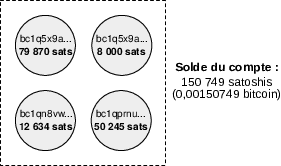
\includegraphics{chapters/img/coins-utxos-account.png}

}

\caption{Examples of coins held by the same account.}

\end{figure}%

This coin-based representation model allows us to view the transaction
mechanism as a coin minting process. Each transaction involves melting
together one or more bitcoin coins in inputs and minting one or more
coins in outputs. This is how Bitcoin's distributed timestamp server
replaces the centralized digital minting present in eCash and RPOW, for
example, which allowed systematic replacement of coins.

Constructing a transaction involves gathering coins of sufficient value
in inputs to melt them and mint new ones. Generally, two coins are
created: the first is sent to the address provided by the recipient to
make the payment (primary output), and the second is sent back to one of
the sender's addresses to ``give themselves change'' (change output).
The difference between the input amount and the output amount is
accounted for in the miner's reward as transaction fees.

Let's consider some examples while ignoring these fees and assuming
Alice wants to make a payment. If Alice has a coin of 12 mBTC (0.012
BTC) and wants to give 7 mBTC to Bob, she must construct and sign a
transaction using this 12 mBTC coin as input, and outputs of 7 mBTC to
Bob's address and 5 mBTC back to her own address. This transaction is
represented in Figure~\hyperref[fig:transaction-1i-2o]{12.2}.

\begin{figure}

{\centering 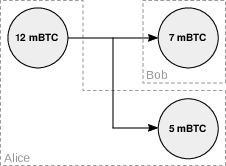
\includegraphics{chapters/img/transaction-1i-2o.png}

}

\caption{Diagram of a transaction with 1 input and 2 outputs.}

\end{figure}%

If Alice doesn't have a coin with a face value greater than 7 mBTC, she
must gather coins to collect sufficient input amount, for example, a
coin of 6 mBTC and one of 2 mBTC. As before, she must create a change
output back to herself to give herself the change. In this case,
illustrated in Figure~\hyperref[fig:transaction-2i-2o]{12.3}, one can
deduce by observing the transaction that the 7 mBTC coin is the payment
result, as it would be economically irrational to merge multiple coins
to send 1 mBTC.

\begin{figure}

{\centering 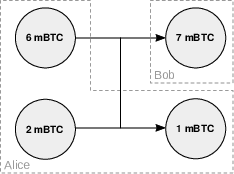
\includegraphics{chapters/img/transaction-2i-2o.png}

}

\caption{Diagram of a transaction with 2 inputs and 2 outputs.}

\end{figure}%

If Alice wishes to transfer all her funds to another account, she
gathers all her coins (6 mBTC, 4 mBTC, 2 mBTC) to send them to a single
address, as shown in Figure~\hyperref[fig:transaction-3i-1o]{12.4}. This
is called a wallet consolidation, which can be identified by an external
observer due to the uniqueness of the output.

\begin{figure}

{\centering 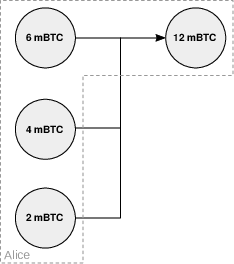
\includegraphics{chapters/img/transaction-3i-1o.png}

}

\caption{Diagram of a transaction with 3 inputs and 1 output.}

\end{figure}%

We see that transactions are not raw transfers from one address to
another but combinations and divisions of digital coins. This
functioning is somewhat counterintuitive but proves useful for the
system's scalability by allowing independent processing of coins, and
for user confidentiality by not encouraging the consolidation of funds
on a single address and facilitating the implementation of anonymization
techniques like coin mixing. This model is therefore particularly suited
to monetary use.

\section*{The Virtual Machine}\label{the-virtual-machine}
\addcontentsline{toc}{section}{The Virtual Machine}

\markright{The Virtual Machine}

The scripts within transactions make Bitcoin a system of programmable
money. These scripts allow embedding various spending conditions, also
called clauses, that go beyond requiring a simple signature, such as
knowing a secret, waiting for a specific time period, or producing
multiple signatures.

Bitcoin's implementation creates an abstract machine whose operation is
replicated on all nodes of the network thanks to the consensus
algorithm. It is simulated via software implementation, hence referred
to as a virtual machine. More precisely, it is a state machine, whose
current state is the set of existing coins---that is, the set of unspent
transaction outputs (UTXOs)---and whose transitions are the transactions
that destroy coins to create new ones. These transactions are assembled
into blocks that are validated at regular intervals by miners. The
propagation of a block across the network updates the state of the
virtual machine, which is (except in the case of a fork) shared by all
nodes.

Within a transaction, unlocking coins is done by executing scripts. The
scripts are predicates in the mathematical sense---that is, incomplete
expressions that become propositions that can be evaluated when
completed by one or more elements. Thus, spending consists of combining
the locking script of the previous output and the unlocking script, and
executing them one after the other: the unlocking script first, followed
by the locking script. Using the coin as a transaction input is approved
if the execution succeeds.

The scripts are written in Bitcoin's internal programming language,
designed by Satoshi Nakamoto in 2008 and unimaginatively named
``Script.'' This programming language functions similarly to Forth, a
language used in the 1970s and 1980s. It is based primarily on two data
stacks, which are data structures operating on the ``last in, first
out'' (LIFO) principle. The language essentially acts on the primary
stack, making it the most important; the secondary stack allows data to
be set aside during script execution.

Satoshi Nakamoto included this scripting system in Bitcoin to enable it
to handle a wide variety of use cases. In June 2010, in response to
Gavin Andresen, he wrote on the forum:

``The nature of Bitcoin is such that, from version 0.1 launched, its
basic operation was set in stone for the rest of its existence. That's
why I wanted to design Bitcoin to support all the transaction types I
could think of. The problem was that each type required special support
code and data fields, whether used or not, and could only cover one
special case at a time. It would have been an explosion of special
cases. The solution was script, which generalized the problem so that
contracting parties could describe their transactions as predicates that
network nodes evaluated. The nodes only need to understand the
transaction to the extent of evaluating whether the sender's conditions
are met\footnote{Satoshi Nakamoto, \emph{Re: Transactions and Scripts:
  DUP HASH160 ... EQUALVERIFY CHECKSIG}, June 17, 2010, 18:46:08:
  \url{https://bitcointalk.org/index.php?topic=195.msg1611\#msg1611}.}.''

The language consists of more than a hundred operators, also called
opcodes, which act on the primary stack in one way or another. The
operators are numbers encoded on 1 byte (ranging from 0 to 255) but are
usually designated by a name describing their function to make reading
more understandable to humans. They are written in uppercase and are
often prefixed with \texttt{OP\_}, though the prefix can be omitted when
unambiguous. For example, the operator that verifies a signature
(\texttt{0xac}) is noted \texttt{OP\_CHECKSIG} or \texttt{CHECKSIG}.

Operators ranging from 1 to 75, sometimes noted as OP\_PUSHBYTES\_X, act
by pushing data of sizes ranging from 1 to 75 bytes onto the stack.
Using additional specific operators (noted OP\_PUSHDATA\_Y) allows for
placing larger information onto the stack. Although this notation can be
used, it is generally simpler to enclose an element in angle brackets to
indicate that it is pushed onto the stack. For example, writing
\texttt{\textless{}signature\textgreater{}} within a script means that
the signature is pushed onto the stack.

The value returned at the end of script execution is a boolean, so the
script can be valid---in which case spending the coin is approved---or
invalid, in which case the transaction is rejected entirely. The script
is valid if and only if the value \texttt{TRUE} (``true'') is present at
the top of the stack at the end of execution. It is invalid if this is
not the case or if its execution halted before completion.

However, the Script language is limited. Nothing in its basic design
allows for loops or access to data outside the transaction, unlike
Ethereum's language, which is nearly Turing-complete. This peculiarity
means it is less flexible but has the advantage of being simpler to
understand and thus more secure.

A typical script example, presented by Andreas Antonopoulos\footnote{Andreas
  M. Antonopoulos, ``\emph{Transactions},'' in \emph{Mastering Bitcoin:
  Programming the Open Blockchain}, 2nd edition, 2017, pp.~117--148.},
involves solving a simple equation involving addition. If we consider
the equation (17 + x = 38), the corresponding locking script is:

\begin{verbatim}
<17> ADD <38> EQUAL
\end{verbatim}

Anyone knowing the answer can spend the coin, which is admittedly not
very secure. The spend requires providing the unlocking script
containing only the solution to the equation, namely 21:

\begin{verbatim}
<21>
\end{verbatim}

The successive execution of these two scripts (see
Figure~\hyperref[fig:bitcoin-stack]{12.5}) proceeds as follows: 1)~the
value 21 is placed on the stack; 2)~the value 17 is placed above it;
3)~the \texttt{OP\_ADD} operator adds the two top values on the stack
and replaces them with their sum, here 38; 4)~the value 38 is placed at
the top of the stack; 5)~the \texttt{OP\_EQUAL} operator compares the
two top values on the stack and replaces them with the equality boolean,
here \texttt{TRUE}. The script execution is thus successful.

\begin{figure}

{\centering 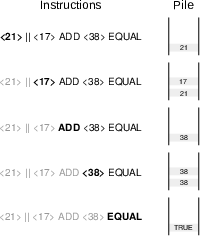
\includegraphics{chapters/img/bitcoin-stack-example.png}

}

\caption{Execution of an addition script on the data stack.}

\end{figure}%

If the value had been different, say 22, the last operation would have
returned the boolean \texttt{FALSE}, and the spend transaction would
have been invalidated.

Many different spending conditions can be implemented with this system.
Some of these conditions are simple, such as knowing a specific secret
or producing a valid signature corresponding to a particular public key.
Verifying knowledge of a secret (whose hash is specified in the UTXO) is
done with the following scripts that push the secret onto the stack,
hash it with SHA-256, and compare the result to the hash:

\begin{verbatim}
<secret> SHA256 <hash> EQUAL
\end{verbatim}

Similarly, verifying the validity of a signature is achieved with the
following scripts that push the signature, then the public key onto the
stack before checking their correspondence:

\begin{verbatim}
<signature> <public key> CHECKSIG
\end{verbatim}

Moreover, there are more advanced conditions like timelocks. These allow
funds in the coin to be locked until a specific date (absolute timelock)
or for a specified duration (relative timelock). The former is
implemented via the \texttt{OP\_CHECKLOCKTIMEVERIFY} operator, whose
technical specifics are described in BIP-65. The latter is applied by
the \texttt{OP\_CHECKSEQUENCEVERIFY} opcode described in BIP-112.

\section*{Classic Schemes}\label{classic-schemes}
\addcontentsline{toc}{section}{Classic Schemes}

\markright{Classic Schemes}

The Script language allows for various diverse and varied
functionalities. In Bitcoin's early days, the system was relatively free
and allowed people to write whatever they wanted in scripts without
discrimination. However, this situation was considerably risky. The main
reason was that the functioning of opcodes had not yet been verified and
tested, as demonstrated by the discovery in July 2010 of a vulnerability
enabled by certain binary operators (CVE-2010-5137). This is why, at the
end of 2010, under Gavin Andresen's initiative, it was decided to
restrict the system's programmability\footnote{Gavin Andresen, \emph{svn
  r197: IsStandard check for transactions}, December 7, 2010, 13:58:33
  UTC:
  \url{https://bitcointalk.org/index.php?topic=2129.msg27744\#msg27744}.}.

This restriction was applied by imposing standard script schemes, which
meant that nodes configured by default would no longer relay
transactions containing scripts that did not comply with this standard.
Thus, this was not a restriction of the global consensus rules but of
the local mempool rules that apply to transaction transmission. Standard
schemes that made things simpler and safer were developed over the
years. As of 2023, the standard transaction output schemes numbered
eight: P2PK, P2PKH, P2MS, P2SH, NULLDATA, P2WPKH, P2WSH, and P2TR.

\subsection{P2PK: Pay to Public Key}\label{p2pk-pay-to-public-key}

The first scheme is Pay to Public Key (P2PK), which can be literally
translated as ``pay to the public key.'' It involves creating a coin
linked to the recipient's public key, which only they can spend by
signing with their private key. The locking script enabling this type of
payment is:

\begin{verbatim}
<public key> CHECKSIG
\end{verbatim}

The presence of the public key explains why ``scriptPubKey'' is
sometimes used to refer to the locking script in general, regardless of
its content.

At the time of spending, the recipient must use an unlocking script
containing simply their signature:

\begin{verbatim}
<signature>
\end{verbatim}

The presence of the signature in this script explains why ``scriptSig''
is sometimes used to refer to the unlocking script in general,
regardless of its content. The successive execution of these two scripts
allows, as we've seen, to verify that the signature provided by the user
corresponds to their public key, making it valid.

The P2PK scheme was used in Bitcoin's early days for receiving payments
by IP (P2IP) and for collecting mining rewards. It has now fallen into
disuse in favor of a rival scheme: P2PKH.

\subsection{P2PKH: Pay to Public Key
Hash}\label{p2pkh-pay-to-public-key-hash}

The Pay to Public Key Hash (P2PKH) scheme, literally translated as ``pay
to the hash of the public key,'' is the second type of receipt format
that appeared in Bitcoin from the beginning due to Satoshi Nakamoto's
design. This scheme allows for a payment not to a public key but to a
hash of a public key, while ensuring that the interpreter still verifies
the validity of the signature concerning the public key when spending
the funds. The public key hash is considered the essential data
(``payload'') of the address, which in this case always begins with a 1,
such as 1FjBKPQ7MTiPSDkJ2ZwPgAXUKQ8yoGbVJX. The locking script here is:

\begin{verbatim}
DUP HASH160 <public key hash> EQUALVERIFY CHECKSIG
\end{verbatim}

And the unlocking script is:

\begin{verbatim}
<signature> <public key>
\end{verbatim}

The execution of the two scripts allows: 1) verifying that hashing the
public key with the HASH-160 function equals the hash specified in the
script; 2) verifying that the signature corresponds to the public key.

The advantage of this scheme is that it allows for shorter addresses
(the information to encode is only 20~bytes instead of 33 or 65 bytes
for a public key), which is why Satoshi Nakamoto implemented it.
Additionally, by not revealing the public key until the time of
spending, this scheme increases security against the very hypothetical
threat of quantum computers.

\subsection{P2MS: Pay to MultiSig}\label{p2ms-pay-to-multisig}

The Pay to MultiSig (P2MS) scheme, meaning ``pay to multisignature,'' is
a multiparty signature scheme requiring the signatures of M people among
N predetermined participants (``M-of-N''). It was standardized in a form
limited to 3 participants in March 2012 with the release of version
0.6.0 of the software. The locking script is as follows:

\begin{verbatim}
M <public key 1> ... <public key N> N CHECKMULTISIG
\end{verbatim}

The corresponding unlocking script is:

\begin{verbatim}
<dummy (0)> <signature 1> ... <signature M>
\end{verbatim}

The presence of the dummy (usually 0) is due to a defect in Satoshi's
implementation of the execution of the \texttt{OP\_CHECKMULTISIG}
operator, which requires one extra element. Developers did not deem it
appropriate to fix this defect, as the correction would have been a hard
fork.

This scheme, particularly demanding in terms of setup, motivated the
creation of the P2SH scheme.

\subsection{P2SH: Pay to Script Hash}\label{p2sh-pay-to-script-hash}

The Pay to Script Hash (P2SH) scheme, which can be literally translated
as ``pay to the script hash,'' extends the idea behind P2PKH, with the
only difference being that the hashed data is not a public key but the
script itself! The script in question is then called the redeem script
to differentiate it from the unlocking script. Its hash is the essential
data of the address, which always begins with a 3, like
3K8Ps6Ayw5ZaKDaLZjfGo3mTgDsc1VXZ8d.

This scheme allows the user to include any script without discrimination
on its format, provided it respects certain limits. It also enables
receiving funds from almost all existing wallets, with the burden of
constructing and unlocking the script falling solely on the recipient
and not shared with the sender, as in the case of using raw scripts.

The locking script for the P2SH scheme is:

\begin{verbatim}
HASH160 <redeem script hash> EQUAL
\end{verbatim}

And the unlocking script is a script of the form:

\begin{verbatim}
[unlocking elements] <redeem script>
\end{verbatim}

The execution of P2SH is more complex than previous schemes, which can
be explained by the context in which it was developed. The idea of
implementing a script scheme that uses a script hash like the public key
hash in P2PKH emerged in 2011 through several proposals. It became more
concrete with Nicolas van Saberhagen's proposal of the \texttt{OP\_EVAL}
operator on October 2---a code operation that allowed recursive
execution of a script within another script\footnote{Nicolas van
  Saberhagen (ByteCoin), \emph{OP\_EVAL proposal}, October 2, 2011,
  00:49:19 UTC:
  \url{https://bitcointalk.org/index.php?topic=46538.msg553689\#msg553689}.}.
Gavin Andresen explained how to make it a soft fork by replacing the
no-effect instruction \texttt{OP\_NOP1}\footnote{Gavin Andresen,
  \emph{Re: OP\_EVAL proposal}, October 2, 2011, 20:42:32 UTC:
  \url{https://bitcointalk.org/index.php?topic=46538.msg554620\#msg554620}.}.

The \texttt{OP\_EVAL} operator was intended to form a new standard
scheme. The locking script would have been:

\begin{verbatim}
DUP HASH160 <redeem script hash> EQUALVERIFY EVAL
\end{verbatim}

while the unlocking script would have been the same as for P2SH. The
successive execution of these two scripts would have allowed, first,
verifying the hash of the redeem script matches the specified hash;
then, in a second step, executing the redeem script and combining it
with the unlocking elements. However, this solution was not accepted,
being judged too dangerous because of its recursion power. An
alternative model, more restrictive, was preferred: P2SH.

The execution of P2SH works exactly like the scheme related to
\texttt{OP\_EVAL}, except that part of the script is not explicitly
indicated. On one hand, verifying the correspondence between the
specified hash and the redeem script is done by the locking script. On
the other hand, the evaluation of the redeem script is performed
implicitly thanks to an exception added to the source code, causing
network nodes recognizing the scheme to interpret it differently. In
Bitcoin Core, this condition can be observed within the VerifyScript
function of the interpreter.

The proposal was codified in BIP-16. While this solution is practical,
it creates complexity and is not very elegant. As Gavin Andresen said in
the introductory explanation of this BIP:

``Recognizing a `special' form of scriptPubKey and performing additional
validation when it is detected is ugly. However, the general consensus
is that the alternatives are either even uglier, more complex to
implement, and/or dangerously extend the language's expressive
power\footnote{Gavin Andresen, \emph{BIP-16: Pay to Script Hash},
  January 3, 2012:
  \url{https://github.com/bitcoin/bips/blob/master/bip-0016.mediawiki\#rationale}.}.''

The P2SH scheme was eventually activated on April 1, 2012, as a soft
fork, despite notable opposition from Luke-Jr, who proposed an
alternative operator, \texttt{OP\_CHECKHASHVERIFY}, described in BIP-17.

\subsection{NULLDATA}\label{nulldata}

The NULLDATA scheme, literally meaning ``insignificant data,'' is a
scheme for embedding arbitrary data on the chain. It is the fourth
classic scheme and was standardized with the arrival of version 0.9.0 of
Bitcoin Core in March 2014. It is based on the \texttt{OP\_RETURN}
instruction, whose effect is to terminate script execution and render
the corresponding coin unspendable\footnote{The \texttt{OP\_RETURN}
  instruction initially returned the value at the top of the stack,
  hence its name. However, in July 2010, the discovery of the ``\emph{1
  RETURN bug}'', which allowed spending any transaction output via the
  unlock script \texttt{TRUE\ RETURN}, prompted Satoshi Nakamoto to
  disable this functionality by making it return \texttt{FALSE}
  systematically. See Satoshi Nakamoto, \emph{reverted makefile.unix
  wx-config -- version 0.3.6 (git commit)}, July 29, 2010, 18:27:12 UTC:
  \url{https://sourceforge.net/p/bitcoin/code/119/}.}. The locking
script of the scheme always begins with \texttt{OP\_RETURN} and is
followed by the pushed data:

\begin{verbatim}
RETURN [arbitrary data]
\end{verbatim}

The output containing this script is exempt from the standard dust
limit, which is currently 546 satoshis for P2PKH outputs, allowing it to
be 0 satoshis. Moreover, due to their inherently unspendable nature,
outputs can be pruned from nodes' UTXO sets. All this makes this scheme
the standard means of inscribing information on the ledger.

\section*{Types of Signatures}\label{types-of-signatures}
\addcontentsline{toc}{section}{Types of Signatures}

\markright{Types of Signatures}

The programmability of Bitcoin is not only derived from its programming
language but also from the signature system, which allows selecting
which part of the transaction is signed. This aspect of programmability
is implemented through the existence of an indicator, called the
signature hash type or \emph{sighash}, which is added to the unsigned
transaction and then to the signature itself. This indicates which part
of the transaction should be hashed before being submitted to the
signing algorithm, hence its name.

The signature type is constructed from several signature flags that can
be combined. The four existing signature flags are:

\begin{itemize}
\tightlist
\item
  \texttt{SIGHASH\_ALL} (\texttt{0x01}), indicating that all outputs are
  signed;
\item
  \texttt{SIGHASH\_SINGLE} (\texttt{0x03}), allowing only a single
  output to be signed;
\item
  \texttt{SIGHASH\_NONE} (\texttt{0x02}), indicating that no outputs are
  signed;
\item
  \texttt{SIGHASH\_ANYONECANPAY} (\texttt{0x80}), allowing only a single
  input to be signed.
\end{itemize}

The three flags concerning outputs can be associated with
\texttt{SIGHASH\_ANYONECANPAY}, allowing for six different signature
types in total, represented in
Figure~\hyperref[fig:signature-hash-types]{12.6}. The most frequent
signature type is obviously \texttt{SIGHASH\_ALL}, although some other
types can occasionally be useful. Notably,
\texttt{SIGHASH\_ALL\ \textbar{}\ SIGHASH\_ANYONECANPAY} allows
constructing \emph{anyone-can-pay} transactions, whose outputs are
determined but where each participant can sign their own input without
knowing the others.

\begin{figure}

{\centering 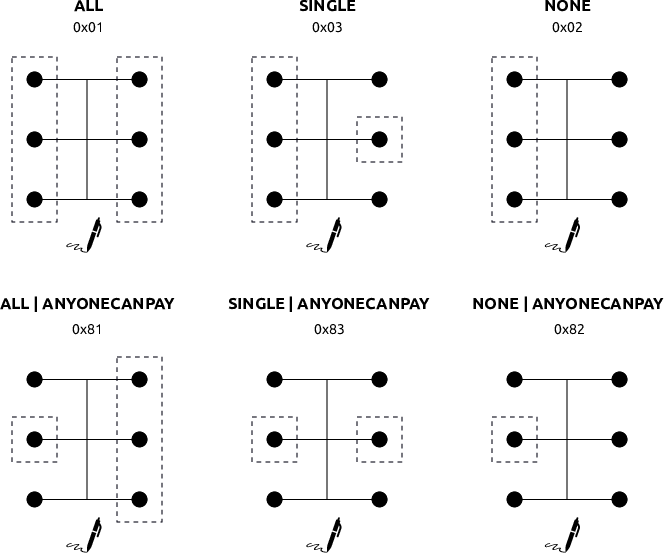
\includegraphics{chapters/img/signature-hash-types.png}

}

\caption{The different signature types in Bitcoin.}

\end{figure}%

These flags were implemented from the beginning by Satoshi Nakamoto
within the prototype. One was logically missing, which Satoshi Nakamoto
probably deemed unnecessary: the one that didn't sign any inputs.
However, with the development of payment channels for the Lightning
Network, developers realized it could be useful. In this spirit, the
\texttt{SIGHASH\_NOINPUT} flag was proposed in February 2016 by Joseph
Poon\footnote{Joseph Poon, \emph{{[}bitcoin-dev{]} SIGHASH\_NOINPUT in
  Segregated Witness}, February 26, 2016, 01:07:46 UTC:
  \url{https://lists.linuxfoundation.org/pipermail/bitcoin-dev/2016-February/012460.html}.}.

This signature type could be partially implemented in BTC through
BIP-118, which provides for the integration of two new flags within
Taproot scripts: \texttt{SIGHASH\_ANYPREVOUT} and
\texttt{SIGHASH\_ANYPREVOUTANYSCRIPT}. It would improve the functioning
of the Lightning Network by implementing the Eltoo protocol, which
relies on the construction of floating transactions.

\section*{SegWit: The Segregated
Witness}\label{segwit-the-segregated-witness}
\addcontentsline{toc}{section}{SegWit: The Segregated Witness}

\markright{SegWit: The Segregated Witness}

SegWit, short for \emph{Segregated Witness}, is a protocol upgrade that
took place on Litecoin-LTC and Bitcoin-BTC in 2017. It involved
separating the unlocking data of transaction inputs, such as signatures,
into a separate data structure called the witness (\emph{witness}) to
eliminate transaction malleability. SegWit thus constituted a profound
restructuring of transactions.

Beyond correcting malleability, SegWit brought increased transaction
capacity and script versioning to facilitate future upgrades. It also
improved the signing algorithm to avoid redundant hashing during
verification and to make offline signing more secure.

\subsection{Malleability}\label{malleability}

SegWit originates from the problem of transaction malleability, an issue
identified since January 2012. In Bitcoin, transactions are malleable in
the sense that they can be slightly modified after their broadcast
without becoming invalid in the eyes of the network. This property stems
from the fact that a signature cannot include itself and, consequently,
the unlocking script is not signed with the rest of the transaction.
Malleability can thus take two forms: malleability intrinsic to the
ECDSA algorithm, which is based on a random number to produce a
signature (malleability by the signer); malleability arising from the
form of inputs' signatures and unlocking scripts (malleability by a
third party).

Malleability is not prohibitive for fund security, but it allows
modifying the transaction identifier after its publication, which can be
problematic in certain situations. For instance, between February 9 and
11, 2014, Mt. Gox and other exchange platforms suffered attacks
exploiting this transaction malleability. Withdrawal transactions were
modified by attackers, making the platforms' poorly configured software
infrastructure believe that these transactions had not been confirmed.
The hackers saw their accounts re-credited while simultaneously
retaining the withdrawn bitcoins. These attacks led to a total loss of
64,564 bitcoins\footnote{For the malleability attack against Mt. Gox,
  see Ken Shirriff, \emph{The Bitcoin malleability attack graphed hour
  by hour}, February 15, 2014:
  \url{https://www.righto.com/2014/02/the-bitcoin-malleability-attack-hour-by.html}.
  See also Christian Decker, Roger Wattenhofer, \emph{Bitcoin
  Transaction Malleability and MtGox}, March 26, 2014:
  \url{https://arxiv.org/pdf/1403.6676.pdf}.}.

Proposals attempted to correct malleability by a third party by
constraining transaction forms as much as possible. In this spirit,
BIP-62 was created in March 2014, one of whose requirements (the
standard encoding of signatures described in BIP-66) was included in the
consensus rules on July 4, 2015. However, these changes did not apply to
malleability by the signer, creating a demand for a generalized fix.

This malleability meant that any actor participating in a multiparty
signature contract could modify the transaction and thus its identifier
at any time. It significantly hindered the implementation of the
Lightning Network, whose payment channels, as we'll see later, rely on
unpublished transactions that need to be referenced and involve multiple
signatures.

The solution was to exclude the unlocking scripts from the transaction
hash calculation so that a change in these scripts would not affect the
identifier. This idea was initially proposed by Gregory Maxwell in
August 2013 on IRC before being implemented within the alpha version of
the Elements sidechain model, announced on June 8, 2015, by Blockstream.
On the same day, Gregory Maxwell presented this version of Elements
including \emph{Segregated Witness} in a developer seminar in San
Francisco, describing the witness as ``a specific value that is a
concrete proof of an existential assertion\footnote{SF Bitcoin
  Developers, \emph{Sidechains: Bringing New Elements to Bitcoin}
  (video), June 8, 2015:
  \url{https://www.youtube.com/watch?v=Twynh6xIKUc}.}.''

This solution was adapted for Bitcoin in the fall of 2015 to be applied
as a soft fork. The SegWit upgrade was officially introduced to the
community by developer Pieter Wuille on December 7, 2015, during the
Scaling Bitcoin II conference in Hong Kong. Essentially, it involved
moving the unlocking scripts to the transaction's witness. Two
identifiers were then calculated: the classic identifier
(\texttt{txid}), which does not include the witness, and the complete
identifier (noted \texttt{wtxid} for \emph{witness transaction
identifier}), which covers the entire transaction. The complete
identifiers were grouped in a second Merkle tree, the witness tree,
whose root was placed in the block's coinbase transaction, ensuring all
data was committed in the proof-of-work calculation. On the other hand,
transactions and blocks remained valid for nodes that had not been
upgraded.

SegWit has been active since August 24, 2017. The absence of the
unlocking script in the calculation of the classic identifier eliminates
malleability entirely, both by signers and by third parties.

\subsection{Increasing Transaction
Capacity}\label{increasing-transaction-capacity}

SegWit also had the indirect effect of creating an extension block and
increasing transaction capacity. Indeed, nodes following the old rules
did not see the witness, so they did not count it in the block size. The
question then was what limit to place on the witness.

The answer was to invent a new metric to measure the impact of
transactions and blocks on the network: weight, which is a weighted
average of the base size and the witness size. Expressed in weight
units, it is defined as the sum of four times the base size ((s\_b)) and
the witness size ((s\_w)):

\[
w = 4 \times s_b + s_w
\]

It follows a virtual size ((s\_v)) defined as the sum of the base size
and one-quarter of the witness size, that is:
\(s_v = s_b + \frac{s_w}{4}\). The block size limit became a block
weight limit, which was set at 4 million units at the time of the
upgrade and remained the same as of November 2023.

Thus, fees initially calculated in satoshis per byte (sat/B) have, since
SegWit, been measured in satoshis per virtual byte (sat/vB). Miners
select transactions based on this rate to maximize profitability
relative to this limit. This effect is only valid if the limit is
reached.

With SegWit, the idea is to weight the impact of inputs compared to
outputs on fee calculation. If activity reaches the capacity ceiling,
outputs are four times more expensive to record on-chain than the
unlocking scripts contained in the inputs. The upgrade, in addition to
providing a discount that encourages its use, created a disincentive to
burden the UTXO set. The factor of 4 approximates material
weighting\footnote{SegWit Resources, \emph{Why a discount factor of 4?
  Why not 2 or 8?}, January 13, 2017:
  \url{https://medium.com/segwit-co/why-a-discount-factor-of-4-why-not-2-or-8-bbcebe91721e}.}.

This limit of 4 million weight units is indicative. The actual block
size generally does not reach 4~MB due to the shape of transactions. The
data contained in normal transactions are not grouped in the witness, so
they do not fully utilize the permitted block space. For example, taking
a block consisting solely of transactions with 2 inputs and 2 outputs
using SegWit, its actual size would be 1.784~MB\footnote{A transaction
  with 2 inputs and 2 outputs of type P2WPKH measures 372 bytes and
  weighs 834 weight units at most. Thus, it's possible to include 4,796
  transactions in a block, allowing us to calculate its actual size.}.

Transactions where the unlocking data are larger benefit more from this
additional block space. This is the case for transactions using
multisignature, such as payment channel closures. It is possible to
approach the 4~MB size by maximizing the data size contained in the
witness. This was done on February 1, 2023, with the creation of a
3.955~MB block whose witness was used to inscribe an image\footnote{See
  block 774,628, identifier
  0000000000000000000515e202c8ae73c8155fc472422d7593af87aa74f2cf3d,
  whose size was 3,955,272~bytes and which included a transaction
  measuring 3,938,383~bytes on its own.}.

\subsection{Script Versioning}\label{script-versioning}

Finally, the SegWit upgrade introduced script versioning, allowing the
deployment of future upgrades. The version thus indicates which rules
are applied. The first version of SegWit in 2017 used version 0, and the
deployment of Taproot in 2021 was done using version 1.

There are three native output types related to SegWit for now: the
P2WPKH scheme, the P2WSH scheme, and the P2TR scheme.

\subsection{P2WPKH: Pay to Witness Public Key
Hash}\label{p2wpkh-pay-to-witness-public-key-hash}

The \emph{Pay to Witness Public Key Hash} (P2WPKH) scheme, literally
meaning ``pay to the witness hash of the public key,'' is the first
scheme implemented by SegWit. The public key hash is obtained by
standard hashing (SHA-256 followed by RIPEMD-160). The apparent locking
script is then:

\begin{verbatim}
<version (0)> <hash160 of the public key>
\end{verbatim}

This script resembles an anyone-can-spend script that anyone could
spend, but the interpreter adds an additional condition to prevent this.
The output type is detected based on its form: the SegWit version (here
0) and the hash size (here 20 bytes). The version and hash form the
essential information of the address, which is encoded using the Bech32
format and always starts with \texttt{bc1q}, such as
bc1q5x9a0aqmgtrucm4l5n0y8e4kxfy9xm4udhygr2.

The unlocking script is empty. The unlocking data are contained in the
transaction's witness. The part of the witness corresponding to the
input is:

\begin{verbatim}
<2> <signature> <public key>
\end{verbatim}

\subsection{P2WSH: Pay to Witness Script
Hash}\label{p2wsh-pay-to-witness-script-hash}

The \emph{Pay to Witness Script Hash} (P2WSH) scheme, literally
translated as ``pay to the witness script hash,'' is the transcription
of P2SH for SegWit. The hash of the redeem script is obtained by SHA-256
out of concern for a collision in RIPEMD-160 in the case of an address
generated by multiple people\footnote{Gavin Andresen,
  \emph{{[}bitcoin-dev{]} Time to worry about 80-bit collision attacks
  or not?}, January 7, 2016, 19:02:05 UTC:
  \url{https://lists.linuxfoundation.org/pipermail/bitcoin-dev/2016-January/012198.html}.}.
The locking script is:

\begin{verbatim}
<version (0)> <sha256 hash of the redeem script>
\end{verbatim}

Again, this script is apparently anyone-can-spend. The output type is
detected by the interpreter based on its form: the SegWit version (here
0) and the hash size (here 32 bytes). The address is again composed of
these two pieces of information and encoded using the Bech32 format.

The unlocking script is empty. The unlocking data are contained in the
transaction's witness. The part of the witness corresponding to the
input is:

\begin{verbatim}
<number of elements + 1> [unlocking elements] <redeem script>
\end{verbatim}

In both cases, the hash is also called the ``witness program.''

\subsection{Nested Types (P2SH-P2WPKH,
P2SH-P2WSH)}\label{nested-types-p2sh-p2wpkh-p2sh-p2wsh}

SegWit also modified the P2SH format to include new exceptions. These
exceptions correspond to the nested types (\emph{nested}) P2SH-P2WPKH
and P2SH-P2WSH. Their functioning involves including the previous
locking scripts (version + hash) in a P2SH output as redeem scripts. The
redeem script is then executed differently to call upon the data
contained in the witness.

These nested types facilitated the transition to SegWit by allowing
wallets that hadn't been updated to send funds to these addresses. Using
native SegWit addresses remains more advantageous.

\subsection{P2TR: Pay to Taproot}\label{p2tr-pay-to-taproot}

The latest scheme to come into effect is the \emph{Pay to Taproot}
(P2TR) scheme, whose name can be translated as ``pay to Taproot.'' This
scheme allows receiving a payment to an external public key that hides a
private key used to sign fund transfers, or to the root of a Merkle tree
containing contract clauses (MAST). Since the payment destination is a
public key, it is somewhat a return to P2PK. The locking script present
in the transaction output is:

\begin{verbatim}
<version (1)> <Taproot public key>
\end{verbatim}

The public key in question is 32 bytes in size. The version and public
key constitute the elements of the address. The address is encoded using
the Bech32m format, a variant of the Bech32 encoding that corrected a
small bug in checksum calculation. The resulting address always starts
with \texttt{bc1p}, such as
bc1pqlqqhzrg60v5h87r8lugusrddgz0j306shcupthy0tdqaqurwn8qr8qsej.
Unlocking the output is done with a simple signature or by executing the
MAST.

All these major changes make SegWit a profound protocol upgrade that has
brought many things to Bitcoin. The requirement to proceed via a soft
fork explains the form it took, and it can only be understood in the
context in which it was activated. However, this upgrade also brought
significant drawbacks, the two main ones being the technical debt that
increases the cost of maintaining and improving the code, and the
weakening of overall confidentiality due to the emergence of new
partially adopted address types. SegWit was therefore far from a perfect
upgrade.

\section*{Coin Mixing}\label{coin-mixing}
\addcontentsline{toc}{section}{Coin Mixing}

\markright{Coin Mixing}

The fact that transactions are published on the chain leads to
surveillance. As we noted earlier, it is possible to make assumptions to
deduce what is really happening on the chain, assuming the user seeks to
minimize the fees paid within their transactions. These heuristics (such
as the co-spending heuristic, the change output heuristic, or the wallet
fingerprint heuristic) form the basis of a discipline called chain
analysis, which consists of cross-referencing these observations with
the identification of real actors to draw conclusions about their actual
economic activity. This is why the term ``transparency'' of the chain is
sometimes used.

However, this transparency is relative, as the chain's data do not
reveal individuals' identities: the system is pseudonymous in the sense
that it records movements between addresses, not between people.
Bitcoin's privacy model, described by Satoshi Nakamoto in the white
paper in 2008, thus involves keeping secret the link between a person's
identity and their addresses\footnote{``The traditional banking model
  achieves a level of privacy by limiting access to information to the
  parties involved and the trusted third party. The need to publicly
  announce all transactions precludes this method but privacy can still
  be maintained by breaking the flow of information elsewhere: by
  keeping public keys anonymous. The public can see that someone is
  sending an amount to someone else but without information linking the
  transaction to anyone.'' --- Satoshi Nakamoto, \emph{Bitcoin: A
  Peer-to-Peer Electronic Cash System}, October 31, 2008.}.

\begin{figure}[H]

{\centering 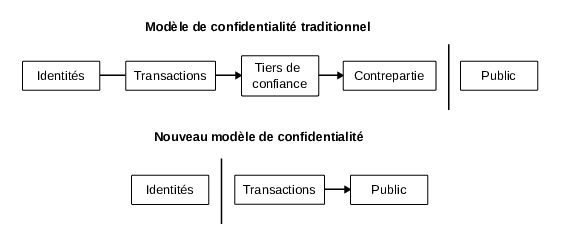
\includegraphics{chapters/img/white-paper-privacy-model-fr.png}

}

\caption{Privacy model presented in the Bitcoin white paper.}

\end{figure}%

This privacy model has obvious weaknesses: accidental information leaks,
which always occur in digital contexts, and voluntary disclosure of the
user's identity by their exchange counterpart. Therefore, no one can
claim to engage in completely secret activity that entirely escapes
surveillance. This is why methods exist to limit the impact of these
revelations to restore one's privacy confidently.

The first measure is the one-time use of addresses. It involves
generating a new private key and a new address for each incoming or
outgoing payment. The benefit of this practice is to reduce the impact
of identity linkage on overall privacy: as long as the address is not
linked to others through on-chain activity (such as co-spending), the
information leak is limited to that address alone. This good practice,
mentioned in the white paper\footnote{``As an additional firewall, a new
  key pair should be used for each transaction to keep them from being
  linked to a common owner. Some linking is still unavoidable with
  multi-input transactions, which necessarily reveal that their inputs
  were owned by the same owner. The risk is that if the owner of a key
  is revealed, linking could reveal other transactions that belonged to
  the same owner.'' --- Satoshi Nakamoto, \emph{Bitcoin: A Peer-to-Peer
  Electronic Cash System}, October 31, 2008.}, is now implemented in all
good wallets.

Beyond prevention, there are also methods to correct mistakes. The
best-known of these is coin mixing, which involves combining one's UTXOs
with those of other users to break the deterministic links between coins
and their owners' identities.

Coin mixing was originally handled by centralized mixing services, known
as mixers or tumblers, which received users' bitcoins, merged them, and
sent common bitcoins back to them after a certain time, preferably in
the form of multiple transactions. The first mixer of this type was
BitLaundry, a platform launched in September 2010 by Peter Vessenes.
These services obscured the provenance of bitcoins for an external
observer but not for their operators, who could also seize the bitcoins
in passing, posing a dual risk.

A technique for performing this type of mixing without relying on an
intermediary was developed later: CoinJoin, formally described in August
2013 by Gregory Maxwell\footnote{Gregory Maxwell, \emph{CoinJoin:
  Bitcoin privacy for the real world}, August 22, 2013, 02:32:31 UTC:
  \url{https://bitcointalk.org/index.php?topic=279249.msg2983902\#msg2983902}.}.
This method involves involving coins in a collaborative joint
transaction that breaks the correspondence between inputs and some
outputs. The typical transaction envisioned is one where several users
each sign an input, the same number of outputs have equal amounts, and
the remaining outputs form the change outputs. In this case, as
illustrated in Figure~\hyperref[fig:coinjoin-transaction]{12.7}, the
change outputs are still linked to the inputs, unlike the primary
outputs which are indistinguishable from each other.

\begin{figure}

{\centering 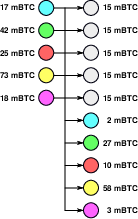
\includegraphics{chapters/img/coinjoin-transaction-5i-10o.png}

}

\caption{Example of a CoinJoin transaction with 5 users.}

\end{figure}%

These mixes rely on the notion of an ``anonymity set,'' which measures
the difficulty of linking an input to an output at a given time. We can
thus obtain a forward-looking score, which is the number of possible
output coins to which an input coin may correspond. In our example
illustrated in Figure~\hyperref[fig:coinjoin-transaction]{12.7}, the
forward-looking score of the output at the time of the transaction is 5.
If the coin had undergone a new mix (as done in Whirlpool), it would
have had a forward-looking score of 9. Similarly, if one or more of the
other coins had been included in a new mix, the score of the observed
coin would have increased accordingly. We can also calculate a
backward-looking score, corresponding to the number of potential input
coins to which a particular output may be linked, assumed to be 5 in our
simple transaction but which can be much higher if one or more coins
have already been mixed multiple times\footnote{Loïc Morel,
  \emph{Understanding and Using CoinJoin on Bitcoin}, July 19, 2022:
  \url{https://www.pandul.fr/post/comprendre-et-utiliser-le-coinjoin-sur-bitcoin}.}.

To manage this, the system typically uses a protocol that allows
participants to connect anonymously via a coordinator without risk of
information leakage or fund theft. The most well-known is ZeroLink,
developed by Adam Ficsor and William Hill in August 2017, a protocol
that uses David Chaum's blind signature process\footnote{Adam Ficsor
  (nopara73), William Hill (TDevD), \emph{ZeroLink: The Bitcoin
  Fungibility Framework}, August 14, 2017:
  \url{https://github.com/nopara73/ZeroLink/tree/32ad53927a343383534bea28fffb098af65fe62a}.}.
In this sense, CoinJoin is sometimes referred to as Chaumian CoinJoin. A
classic implementation of this idea has been realized by Whirlpool
(Samourai Wallet\footnote{The Whirlpool mixing system and the Samourai
  wallet were shut down on April 24, 2024, by order of the United States
  Department of Justice. The co-founders of these services, Keonne
  Rodriguez and William Hill, were arrested the same day by authorities.
  --- United States Attorney for the Southern District of New York,
  \emph{Founders And CEO Of Cryptocurrency Mixing Service Arrested And
  Charged With Money Laundering And Unlicensed Money Transmitting
  Offenses}, April 24, 2024:
  \url{https://www.justice.gov/usao-sdny/pr/founders-and-ceo-cryptocurrency-mixing-service-arrested-and-charged-money-laundering}.
  (Note from January 2025.)}) and Wasabi 1.0. Additionally, variants
(CoinShuffle, CoinShuffle++, CashShuffle, CashFusion) have been
implemented on Bitcoin variants like Decred or Bitcoin Cash. More
recently, the Wasabi wallet integrated Wabisabi, which allows mixing
with arbitrary output values, complicating the estimation of the privacy
provided but avoiding the need to manage change outputs separately.

However, collaborative transactions are not limited to CoinJoin. For
example, there is another method called PayJoin, allowing the merchant
to perform a mix with the customer at the time of payment by involving
one or more coins as inputs. This operation has the effect of misleading
chain analysis by making an external observer believe that a single user
has combined their inputs, masking the actual payment amount.

Returning to our example of Alice paying 7 mBTC to Bob by combining two
coins of 6 and 2 mBTC to reach a sufficient input amount. In this case,
as shown in Figure~\hyperref[fig:payjoin-transaction]{12.8}, the
application of PayJoin involves the merchant including one or more of
their own coins as inputs, increasing the amount sent to the destination
output accordingly, for example, 7 mBTC.

\begin{figure}

{\centering 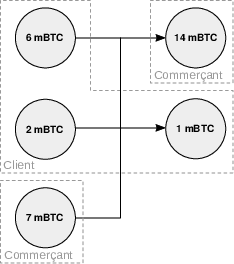
\includegraphics{chapters/img/payjoin-transaction-3i-2o.png}

}

\caption{Example of a PayJoin transaction.}

\end{figure}%

This technique was conceptualized in 2018 in several independent ways,
notably through the Pay-to-EndPoint (P2EP) payment protocol and Samourai
Wallet's Stowaway transactions. Their implementation occurred in 2019
for Stowaway transactions and in 2020 for P2EP.

Finally, another method aligning with the logic of coin mixing is
Coinswap, a process developed by Chris Belcher that allows two or more
users to exchange their coins without needing to trust each other and
without this operation leaving a particular trace on the
chain\footnote{Chris Belcher, \emph{Design for a CoinSwap Implementation
  for Massively Improving Bitcoin Privacy and Fungibility}, May 25,
  2020:
  \url{https://gist.github.com/chris-belcher/9144bd57a91c194e332fb5ca371d0964}.}.
However, this technique has an additional drawback in that one party
inherits the entire history of the other party's coin and must assume
any potential responsibility.

\section*{Other Privacy Techniques}\label{other-privacy-techniques}
\addcontentsline{toc}{section}{Other Privacy Techniques}

\markright{Other Privacy Techniques}

Beyond simple coin mixing to obfuscate paths an external observer might
follow, there are several techniques to enhance Bitcoin's privacy. These
often require modifying the base protocol and represent trade-offs,
which is why they are not necessarily implemented.

These techniques were developed in the years following Bitcoin's
emergence, notably on the Bitcointalk forum. Not being a cryptography
academic, Satoshi Nakamoto primarily focused on the system's robustness
when he designed it and did not seek to include advanced techniques.
However, he was open to any proposals that would make ``a much better,
easier, and more convenient implementation of Bitcoin\footnote{Satoshi
  Nakamoto, \emph{Re: Not a suggestion}, August 11, 2010, 00:14:22 UTC:
  \url{https://bitcointalk.org/index.php?topic=770.msg8637\#msg8637}.}.''

The first technique in this category is the ring signature process,
formalized in 2001 by Ronald Rivest, Adi Shamir, and Yael Tauman. It is
based on the group signature process introduced by David Chaum and
Eugène van Heyst in 1991, which allowed any member of a group to sign a
message on behalf of the group without an external verifier being able
to identify the member, but relied on a central administrator. The ring
signature innovated by not requiring an administrator, setup procedure,
coordination, and not allowing a member to revoke their anonymity.

Regarding cryptocurrency, the principle is as follows: for each input
coin of the transaction, the signer gathers several other coins
available on the chain (called decoy outputs), uses their public keys,
and signs with their private key. They also provide a key image
corresponding to the coin, written on the chain, which ensures that the
same coin is not spent twice. The more outputs involved in the ring, the
larger the anonymity set. The trade-off is that using transaction
outputs as decoys forces nodes to retain the set of these outputs since
it is impossible to know which one was actually spent.

The second technique is stealth addresses, described in 2011 by Nicolas
van Saberhagen and formalized in 2014 by Peter Todd for
Bitcoin\footnote{Nicolas van Saberhagen (ByteCoin), \emph{Untraceable
  transactions which can contain a secure message are inevitable}, April
  17, 2011, 02:34:24 UTC:
  \url{https://bitcointalk.org/index.php?topic=5965.msg87757\#msg87757};
  Peter Todd, \emph{{[}Bitcoin-development{]} Stealth Addresses},
  January 6, 2014, 12:03:38 UTC:
  \url{https://lists.linuxfoundation.org/pipermail/bitcoin-dev/2014-January/004020.html}.}.
It essentially uses the Elliptic Curve Diffie-Hellman key exchange
scheme (ECDH) to generate one-use receiving addresses.

The basic operation is as follows. The recipient generates a private key
and derives a public key they transmit as a meta-address. The sender
generates an ephemeral private key, called the transaction private key,
and calculates the corresponding public key. They can compute a shared
secret from their private key and the other's public key (ECDH). The
sender uses this secret and the recipient's public key to construct a
one-use address and send funds to it, which only the recipient can
spend, provided they know the transaction public key (which can be
stored in a NULLDATA output). Instead of using a single key pair, the
recipient can also use two so that they have separate roles: view keys
and spend keys. The view private key is the only non-public element
involved in constructing the address on the recipient's side and serves
to identify outputs corresponding to the address in question. The spend
private key is, as the name clearly indicates, used to spend the
funds\footnote{In mathematical terms, if we denote (r) and (R) as the
  transaction ephemeral keys, (v) and (V) as the view keys, and (k) and
  (K) as the spend keys, then the meta-address is (M = (K, V)), the
  shared secret is\ldots{}}.

If implemented externally to the protocol, this method's drawback is the
need to scan the entire blockchain to know if one has received a
payment. To avoid this burden, BIP-47 was proposed.

BIP-47 thus formalizes another method akin to stealth addresses, more
complex, which is reusable payment codes, implemented as PayNyms in
Samourai and Sparrow wallets. In this process, the payment codes of two
participants allow deriving receiving addresses through key derivation.
This implies they must know each other's payment codes, and at least one
of these codes must remain secret. The recipient's payment code is
generally public, so the sender's must be hidden. The sender transmits
it encrypted in the form of a notification transaction sent to the
recipient's address. This scheme's major drawback is requiring a
transaction (and paying the associated fee) to add a possible recipient.

A final variant is the silent payments process, proposed in 2022 by
Ruben Somsen\footnote{Ruben Somsen, \emph{Silent Payments}, March 13,
  2022:
  \url{https://gist.github.com/RubenSomsen/c43b79517e7cb701ebf77eec6dbb46b8}.},
which avoids the notification burden by using the public key of one of
the transaction's inputs and reduces the chain scanning burden by
limiting to the UTXO set or a subset like P2TR outputs.

The ring signature technique and stealth address process were combined
in 2013 in the CryptoNote cryptocurrency concept by Nicolas van
Saberhagen\footnote{Nicolas van Saberhagen, \emph{CryptoNote v2.0},
  October 17, 2013: \url{http://cryptonote.org/whitepaper.pdf}; archive:
  \url{https://web.archive.org/web/20140529235502/http://cryptonote.org/whitepaper.pdf}.}.
In it, nodes need to retain the set of transaction outputs (since the
ring signature process obscures the fact that an output has been spent),
and each wallet needs to scan the set of these outputs to see if it has
received a payment. Integrating stealth addresses into the protocol
allows publishing the ephemeral public key directly in the transaction
(making it a transaction key) and avoids the need for notification. The
concept was initially implemented in the highly dubious Bytecoin in
March 2014 before appearing in Monero in April of the same year, which
is now its main representative, notably implementing ring signatures
with 16 members.

The third privacy enhancement technique is Confidential Transactions,
which hides the amounts involved in user exchanges and, logically,
should rather be called Confidential Amounts. The process was described
by Adam Back in 2013 and formalized by Gregory Maxwell in
2015\footnote{Adam Back, \emph{bitcoins with homomorphic value
  (validatable but encrypted)}, October 1, 2013, 14:19:53:
  \url{https://bitcointalk.org/index.php?topic=305791.msg3277431\#msg3277431};
  Gregory Maxwell, \emph{Confidential Transactions}, 2015, archive:
  \url{https://web.archive.org/web/20150628230410/https://people.xiph.org/~greg/confidential_values.txt}.}.
It requires each transaction output to contain a Pedersen commitment
that binds the coin to the recipient's public key without revealing it,
and a range proof, which is a zero-knowledge proof (ZKP) demonstrating
the validity of the amount without disclosing it.

Confidential Transactions were added to Monero in 2017 thanks to the
work of Shen Noether. RingCT, which hides exchanged amounts, was added
to the protocol in January 2017 and made mandatory in September of the
same year. It increased transaction sizes compared to standard
transactions. However, since October 2018, this trade-off has been
mitigated thanks to the implementation of bulletproofs, which reduced
the burden of range proofs and allowed an 80\% reduction in transaction
sizes\footnote{Benedikt Bünz, Jonathan Bootle, Dan Boneh, Andrew
  Poelstra, Pieter Wuille, Gregory Maxwell, \emph{Bulletproofs: Short
  Proofs for Confidential Transactions and More}, 2018:
  \url{https://eprint.iacr.org/2017/1066.pdf}.}.

Another concept using Confidential Transactions is Mimblewimble,
proposed on August 1, 2016, by an anonymous person calling themselves
Tom Elvis Jedusor in the IRC channel \#bitcoin-wizards, where they
shared a link to a descriptive text hosted on Tor\footnote{Tom Elvis
  Jedusor, \emph{Mimblewimble}, July 19, 2016, archive:
  \url{https://download.wpsoftware.net/bitcoin/wizardry/mimblewimble.txt}.}.
Mimblewimble attracted the attention of some Bitcoin developers,
including mathematician Andrew Poelstra, who provided a more advanced
description in a paper dated October 6, 2016\footnote{Andrew Poelstra,
  \emph{Mimblewimble}, October 6, 2016:
  \url{https://download.wpsoftware.net/bitcoin/wizardry/mimblewimble.pdf}.}.

Mimblewimble's contribution is to condense the transaction history by
overhauling transaction structure. It relies on three cryptographic
primitives: Confidential Transactions, which hide amounts; one-way
aggregate signatures (OWAS), which allow combining transactions within a
block; and transaction cut-through, which allows removing intermediary
transaction outputs. This reduction, which modestly improves system
privacy, comes at the cost of programmability, which is directly
rendered impossible.

Mimblewimble was natively implemented in the Grin system developed by
Ignotus Peverell starting in October 2016 and launched on January 15,
2019. Another implementation, also launched in January 2019, was the
Beam network. Mimblewimble was also integrated into Litecoin on May 20,
2022, as a soft fork of an auxiliary block called MWEB for
\emph{MimbleWimble via Extension Blocks}.

Finally, there are other anonymization techniques based on
zero-knowledge proofs. The most well-known were popularized through two
protocols released in 2013 and 2014 by Matthew Green and his students:
Zerocoin and Zerocash\footnote{Ian Miers, Christina Garman, Matthew
  Green, Aviel D. Rubin, ``\emph{Zerocoin: Anonymous Distributed E-Cash
  from Bitcoin}'', in \emph{2013 IEEE Symposium on Security and
  Privacy}, 2013, pp.~397--411:
  \url{https://ieeexplore.ieee.org/document/6547123}; Eli Ben Sasson,
  Alessandro Chiesa, Christina Garman, Matthew Green, Ian Miers, Eran
  Tromer, Madars Virza, ``\emph{Zerocash: Decentralized Anonymous
  Payments from Bitcoin}'', \emph{2014 IEEE Symposium on Security and
  Privacy}, 2014, pp.~459--474:
  \url{https://ieeexplore.ieee.org/document/6956581}.}. The first
protocol, Zerocoin, hides fund provenance. The second protocol hides
provenance, destination, and amounts using zk-SNARKs
(\emph{Zero-Knowledge Succinct Non-Interactive Arguments of Knowledge}).

Zerocoin was implemented in Zcoin in September 2016. Starting in 2019,
Zcoin gradually moved away from Zerocoin by adopting the Sigma and
Lelantus protocols and became Firo in 2020. Zerocash was implemented in
the Zcash system in October 2016. Using zero-knowledge proofs required a
trusted setup of public parameters. While Zcoin's developers chose to
use known parameters, Zcash's decided to organize an event called ``The
Ceremony'' to generate these parameters. This ceremony took place from
October 21 to 23, 2016, bringing together six participants: Andrew
Miller, Peter Van Valkenburgh, Zooko Wilcox-O'Hearn, Derek Hinch, Peter
Todd, and notably Edward Snowden under the pseudonym John
Dobbertin\footnote{Zooko Wilcox-O'Hearn, \emph{The Design of the
  Ceremony}, October 26, 2016:
  \url{https://electriccoin.co/blog/the-design-of-the-ceremony/}.}. This
trusted setup became unnecessary in 2022 with the integration of the
Halo protocol.

In general, all these processes involve trade-offs in scalability
(proofs are heavier than a simple signature), auditability (not seeing
amounts implies having to fully trust the processes and their
implementation), and programmability (programming coins opposes making
them indistinct). This is why they have all been implemented in
alternative versions of Bitcoin and not in its main version (BTC), whose
community is inherently more conservative.

\section*{A Complex Machine}\label{a-complex-machine}
\addcontentsline{toc}{section}{A Complex Machine}

\markright{A Complex Machine}

Bitcoin thus forms a machine that may seem quite complex at first
glance. This complexity can be explained by its objectives and the
events that have marked its technical history. Its primary goal---to be
money---is behind the representation of bitcoins in circulation by
unspent transaction outputs, a representation that facilitates
parallelization and promotes transaction confidentiality (which can be
further enhanced by coin mixing and dedicated cryptographic techniques).

Moreover, Satoshi's desire to automate various mechanisms led him to
integrate a true programming system within the protocol. This allows for
the implementation of autonomous contracts that execute complex
financial interactions between multiple participants. It also indirectly
facilitates the inscription of arbitrary data on the chain. These two
uses (contractual and notarial) form Bitcoin's two secondary use cases,
which we will discuss in the next chapter.

\bookmarksetup{startatroot}

\chapter{Autonomous Contracts}\label{ch:contracts}

A self-executing contract, known in English as a \emph{smart contract},
is a computer program that operates without the need for a trusted third
party. These contracts are also referred to as self-executable contracts
or, literally translated, intelligent contracts. Each contract consists
of clauses that specify particular spending conditions.

Bitcoin represents the first practical implementation of a system
hosting autonomous contracts through its internal programming mechanism
that employs scripts within transactions. This enables the execution of
a variety of contracts, ranging from multisignature accounts to payment
channels and escrow arrangements. The openness provided by this
capability facilitates the inscription of arbitrary data on the chain, a
strictly non-monetary use case of the protocol.

\section*{Simple Contracts}\label{simple-contracts}
\addcontentsline{toc}{section}{Simple Contracts}

\markright{Simple Contracts}

The concept of autonomous contracts\footnote{The term ``contrat
  autonome'' aiming to translate \emph{smart contract} was proposed by
  Jacques Favier, Adli Takkal-Bataille, and Benoît Huguet in
  \emph{Bitcoin: Métamorphoses} (pp.~105--107) in 2018.} emerged within
the cypherpunk movement in the 1990s. It was introduced by Nick Szabo in
1994, who defined it as follows:

``A smart contract is a computerized transaction protocol that executes
the terms of a contract. The general objectives of designing smart
contracts are to satisfy common contractual conditions (such as payment
terms, liens, confidentiality, and even enforcement), minimize
exceptions both malicious and accidental, and minimize the need for
trusted intermediaries\footnote{Nick Szabo, \emph{Smart Contracts},
  1994, archived:
  \url{https://web.archive.org/web/20011102030833/http://szabo.best.vwh.net:80/smart.contracts.html}.}.''

The simplest form of an autonomous contract is value transfer,
containing only one clause: the provision of a digital signature
corresponding to a given public key. However, a multitude of other
contracts can be implemented on Bitcoin, making it impossible to provide
an exhaustive list. Here, we will describe a few examples to explain how
they can be implemented. Let's first examine specific cases such as the
multisignature account, escrow arrangements, crowdfunding, and atomic
swaps.

\subsection{The Multisignature
Account}\label{the-multisignature-account}

A multisignature account is a shared account between multiple entities.
It is based on the multipartite signature scheme described in
Chapter~\hyperref[ch:mechanics]{12}, where spending funds requires M
signatures out of N participants (known as ``M-of-N''). For example,
spending from a 2-of-3 account requires that 2 out of 3 predetermined
participants provide a valid signature, regardless of which individuals
they are.

This type of contract is useful for joint accounts between spouses
(2-of-2), facilitating corporate holdings (e.g., 3 partners out of 7),
or improving the general security of bitcoin storage. Exchanges notably
use this type of contract to manage their assets. As of November 2023,
the world's second-richest address was Bitfinex's 3-of-5 multisignature
address, holding over 178,000~BTC\footnote{Bitfinex's 3-of-5
  multisignature address is
  bc1qgdjqv0av3q56jvd82tkdjpy7gdp9ut8tlqmgrpmv24sq90ecnvqqjwvw97.}.

\subsection{Escrow Arrangements}\label{escrow-arrangements}

An escrow, known in English as \emph{escrow}, is a method that involves
a trusted third party, such as a notary, to secure a transaction between
two parties who are wary of each other. Utilizing Bitcoin's
programmability can reduce the third party's power by including a
limitation in the clause concerning them. This type of contract relies
on two basic technical components: multisignature schemes and timelocks.

Consider the example of two individuals who do not know each other,
Alice and Bob, wanting to conduct an online transaction: Alice is the
buyer, and Bob is the seller. They both engage a trusted intermediary,
Lenny, to create the escrow contract. Alice sends funds to it and waits
to receive the goods. Two clauses can then be activated:

\begin{itemize}
\item
  \textbf{Amicable settlement}: The contract is unlocked by the
  signatures of both parties, who can choose to send the funds to Bob
  (successful exchange) or refund Alice (failed exchange).
\item
  \textbf{Dispute resolution}: After a predetermined period (e.g., 30
  days), the contract can be unlocked by Lenny's signature and that of
  one of the two parties; in this case, Lenny determines who is the
  honest party and sends the funds accordingly.
\end{itemize}

\begin{figure}

{\centering 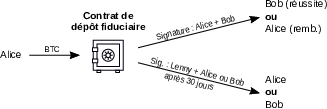
\includegraphics{chapters/img/escrow-contract.png}

}

\caption{Escrow contract.}

\end{figure}%

As depicted in Figure~\hyperref[fig:escrow-contract]{13.1}, this
mechanism encourages both parties to cooperate to avoid delays and
prevents the third party (Lenny) from colluding with either party before
the stipulated period (30 days here). Thus, reliance on trust is
minimized as much as possible.

This type of contract was endorsed by Satoshi Nakamoto in the white
paper\footnote{``Buyers could be easily protected by routine escrow
  mechanisms.''---Satoshi Nakamoto, \emph{Bitcoin: A Peer-to-Peer
  Electronic Cash System}, October 31, 2008.}. Indeed, the
irreversibility of transfers in Bitcoin offered little guarantee for
merchants, and escrow arrangements helped mitigate the problem. This
mechanism is typically involved today in peer-to-peer exchange platforms
like Bisq or Hodl Hodl, even if the implementation differs from what's
presented here.

\subsection{Crowdfunding}\label{crowdfunding}

Crowdfunding involves reaching out to the general public to contribute
to the support of a project, as opposed to financing through bank loans
or raising funds from professional venture capitalists. It is most often
an informal agreement between the project's promoter and the public,
aimed at supporting the creation of a common good that benefits
everyone. In Bitcoin, this agreement can be executed through revocable
payment promises that are not subject to the arbitrariness of a trusted
third party.

Technically, this involves creating a transaction called
``anyone-can-pay,'' where each contributor's signature covers only the
funding output and their own input, allowing additional inputs to be
added (see Figure~\hyperref[fig:sighash-anyonecanpay]{13.2}). The
resulting transaction is valid only if the total inputs reach the
specified output amount, so contributors retain control of their funds
until the total payment is made and can withdraw at any time.

\begin{figure}

{\centering 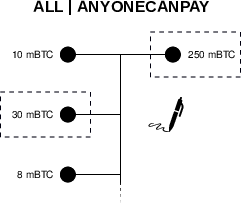
\includegraphics{chapters/img/sighash-anyonecanpay.png}

}

\caption{Crowdfunding transaction.}

\end{figure}%

In the world of open-source software, this type of crowdfunding is
particularly important because there's no privilege associated with
writing code that allows one to make a living by selling licenses. This
is even more true in the world of cryptocurrency, which heavily depends
on the proper maintenance of software implementations. This is why Mike
Hearn, who was closely interested in Bitcoin's programming capabilities,
quickly adopted this possibility to deploy such ``assurance contracts''
allowing for community funding of ecosystem projects. He implemented the
concept in his Lighthouse application, a functional version of which was
released in 2015, aiming to facilitate community support for projects.
With the onset of the block size war, this project was set aside by
Hearn and eventually abandoned. However, the method was later adopted on
Bitcoin Cash in 2020 via Flipstarter, which helped raise significant
sums to fund the protocol's software infrastructure.

\subsection{Atomic Swaps}\label{atomic-swaps}

An atomic swap is a secure way to exchange two cryptocurrencies
operating on different blockchains without using a trusted intermediary.
The term ``atomic'' refers to the indivisible nature (from the ancient
Greek \foreignlanguage{greek}{ἄτομος}, \emph{átomos}) of the exchange:
either both parties transfer their due amounts, or nothing happens. The
concept was described by Sergio Lerner and Gregory Maxwell in July 2012
on the Bitcointalk forum\footnote{Sergio Demian Lerner, \emph{P2PTradeX:
  P2P Trading between cryptocurrencies}, July 5, 2012, 23:49:48 UTC:
  \url{https://bitcointalk.org/index.php?topic=91843.msg1011737\#msg1011737};
  Gregory Maxwell, \emph{Re: P2PTradeX: P2P Trading between
  cryptocurrencies}, July 6, 2012, 02:17:02 UTC:
  \url{https://bitcointalk.org/index.php?topic=91843.msg1011956\#msg1011956}.}.

The atomic swap relies on the concept of a hash time-locked contract
(HTLC), which is a contract with two clauses, meaning the funds can be
unlocked under two conditions\footnote{To ensure the proper execution of
  the contract (avoid transaction replacement during confirmation wait),
  public keys are assigned to each of these conditions so that a
  signature is always required from the recipient of the funds.}:

\begin{itemize}
\item
  \textbf{Mutual agreement}: The revelation of a secret that is hashed
  by a function and compared to the hash embedded in the contract.
\item
  \textbf{Dispute resolution}: Waiting for a certain predetermined lock
  time specified in the contract.
\end{itemize}

Consider an example of an atomic swap between Alice, who has BTC, and
Bob, who has LTC. Alice (\emph{maker}) proposes to exchange 0.03 BTC for
10~LTC, at an exchange rate of 0.003~LTC per BTC, and Bob (\emph{taker})
accepts the deal. This negotiation can occur via a public or private
order book. Alice randomly chooses a secret (denoted \(s\)), a 32-byte
number, whose cryptographic hash \(H(s)\) she provides to Bob. They can
thus each build a contract on their side to perform the atomic swap. The
process is described in
Figure~\hyperref[fig:atomic-swap-contract]{13.3}.

The first phase is the commitment phase. First, Alice constructs, signs,
and broadcasts a commitment transaction sending 0.03~BTC to the atomic
swap contract on the Bitcoin chain. She provides its content and address
to Bob for verification. Then, she constructs and signs a refund
transaction spending the funds from this contract, which she can
broadcast after a predefined delay (here, 16 hours). Once Alice's
commitment transaction is confirmed, Bob does the same on his side: he
creates an equivalent contract on the Litecoin chain, where he sends
10~LTC, and gives its content and address to Alice for her to ensure
everything is in order. Finally, he constructs and signs a transaction
that will refund him after a delay strictly less than Alice's
transaction (here, 8 hours). This difference results from the unbalanced
relationship between Alice (who knows the unlocking secret) and Bob (who
does not).

Once the commitment transactions are confirmed on their respective
chains, the second phase of the atomic swap---the collection phase---can
begin. Alice constructs, signs, and broadcasts a transaction that allows
her to retrieve Bob's 10~LTC. To do this, she provides the secret within
the transaction, thereby revealing it to Bob. Finally, Bob can also
construct, sign, and broadcast a transaction that grants him the
0.03~BTC to his account. In this way, the exchange is completed!

\begin{figure}

{\centering 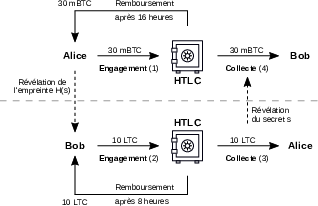
\includegraphics{chapters/img/atomic-swap-contract.png}

}

\caption{Contracts and transactions in an atomic swap.}

\end{figure}%

This model ensures that neither participant can refund themselves before
the end of Bob's lock time (8 hours); that Alice cannot assert her
refund transaction at the time of broadcasting her collection
transaction; and that Bob cannot appropriate Alice's funds until she has
broadcast her transaction. These guarantees make the process logically
secure, even if disruptive events can occur, such as increased
confirmation times due to fee market volatility.

The first real atomic swap was conducted between Litecoin and Decred on
September 19, 2017, by Charlie Lee and Alex Yocom-Piatt\footnote{The
  contract addresses on LTC and DCR were (respectively)
  MLp49daA411aoZ1TmGEdyLuTCE9YA6xhpc and
  DccPF1yt9cV8vhr97fq3umBx7RqV53MYGDY. The exchange was 1.337~LTC for
  2.4066~DCR.---\emph{Decred-compatible cross-chain atomic swapping},
  September 20, 2017:
  \url{https://github.com/decred/atomicswap/blob/master/README.md\#first-mainnet-dcr-ltc-atomic-swap}.}.
Today, atomic swaps are rare, and the order books of specialized
platforms like AtomicDEX are sparsely populated. However, with the
tightening regulations affecting the ecosystem and making centralized
platforms less reliable, it's possible they will play a major role in
the future.

\section*{Payment Channels}\label{payment-channels}
\addcontentsline{toc}{section}{Payment Channels}

\markright{Payment Channels}

A particular application of autonomous contracts in Bitcoin is the
deployment of payment channels. A payment channel allows two users to
make repeated bitcoin payments securely and instantly without publishing
transactions on the blockchain, using previously locked funds. These
channels are fundamental to the Lightning Network, built as a layer on
top of the chain.

\subsection{Poon-Dryja Payment
Channels}\label{poon-dryja-payment-channels}

Although the idea of a payment channel was envisioned from the early
days, it only materialized with the concept developed by Joseph Poon and
Thaddeus Dryja in their Lightning Network project\footnote{Joseph Poon
  and Thaddeus Dryja, \emph{The Bitcoin Lightning Network DRAFT Version
  0.5}, February 28, 2015:
  \url{https://lightning.network/lightning-network-paper-DRAFT-0.5.pdf}.}.
This concept involves a bidirectional channel whose security relies on a
penalty mechanism. Both participants lock funds in a 2-of-2
multisignature contract and can make payments to each other within the
available liquidity. The sum of both participants' balances is referred
to as the channel capacity.

A channel goes through three phases during its existence:

\begin{itemize}
\item
  \textbf{Opening or setup phase}: Funds are locked by the participants
  into an autonomous 2-of-2 multisignature contract.
\item
  \textbf{Negotiation or update phase}: The distribution of funds within
  the channel is adjusted.
\item
  \textbf{Closing or settlement phase}: Funds are distributed to the
  participants on-chain, usually cooperatively according to the latest
  state of the channel.
\end{itemize}

The initial distribution and channel updates are carried out through
commitment transactions exchanged between the participants and \emph{not
broadcasted} to the network unless a dispute occurs, such as a
non-cooperative closure. These commitment transactions are asymmetric,
meaning each participant has their own version.

Suppose Alice and Bob have a channel, as illustrated in
Figure~\hyperref[fig:poon-dryja-contracts]{13.4}. In this case, Alice's
latest commitment transaction, which can only be finalized and
broadcasted by Bob, accounts for the updated state of the channel and
distributes the funds between Alice's address and a claim contract. This
claim contract contains two clauses:

\begin{itemize}
\item
  \textbf{Recovery by Bob}: After a locktime, Bob can recover the funds,
  distributing them according to the balances indicated in the channel.
\item
  \textbf{Recovery by Alice}: Using a revocation key that is revealed
  later when the channel is updated again, Alice can recover the funds.
\end{itemize}

If a payment occurs from Alice to Bob, the channel update proceeds as
follows. Alice constructs and signs her commitment transaction using
Bob's revocation public key, which he previously provided to her. Only
Bob can finalize and broadcast this transaction. Bob responds by sending
her his revocation private key, rendering Alice's previous commitment
transaction ineffective. The same process occurs symmetrically: Bob
constructs and signs his commitment transaction, sends it to Alice, and
she reveals her revocation private key in exchange, making Bob's prior
commitment transaction powerless\footnote{Andreas M. Antonopoulos,
  Olaoluwa Osuntokun, René Pickhardt, ``Payment Channels,'' in
  \emph{Mastering the Lightning Network: A Second Layer Blockchain
  Protocol for Instant Bitcoin Payments}, O'Reilly Media, 2022,
  pp.~149--184.}.

Revealing the revocation key at each update stage enables a penalty
mechanism at any time. If one of the parties broadcasts a commitment
transaction corresponding to a previous state of the channel, the other
can recover \emph{all} the funds in the channel. For example, Alice
could recover Bob's funds if he were to broadcast a previous channel
state intending to ``undo'' the last payment.

\begin{figure}

{\centering 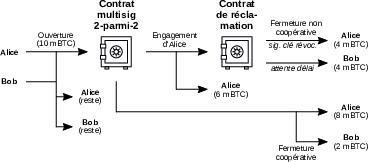
\includegraphics{chapters/img/lightning-poon-dryja-channel-contracts.png}

}

\caption{Contracts and transactions in a Poon-Dryja payment channel:
case of Bob paying 2~mBTC to Alice.}

\end{figure}%

The main drawback of this penalty mechanism is that continuous network
monitoring is required to prevent theft, necessitating a full node or a
well-chosen trusted third party (a ``watchtower'').

This functioning of Poon-Dryja channels also means that any error is
heavily penalized: accidentally broadcasting a prior commitment
transaction leads to the other party recovering the funds. It has other
drawbacks as well: it requires storing all previous channel states,
forces participants to choose transaction fees in advance, and
significantly complicates innovations within the Lightning Network. To
improve this situation, the ``Decker-Russell-Osuntokun'' payment
channels were conceptualized.

\subsection{Decker-Russell-Osuntokun Payment
Channels}\label{decker-russell-osuntokun-payment-channels}

The Decker-Russell-Osuntokun payment channels were described by
Christian Decker, Rusty Russell, and Olaoluwa Osuntokun in a white paper
published in April 2018\footnote{Christian Decker, Rusty Russell,
  Olaoluwa Osuntokun, \emph{eltoo: A Simple Layer2 Protocol for
  Bitcoin}, April 30, 2018: \url{https://blockstream.com/eltoo.pdf}.}.
The underlying protocol is called Eltoo, a play on ``L2'' (signifying
\emph{layer two}).

The functioning of Decker-Russell-Osuntokun channels is based on a chain
of transactions that are not intended to be broadcast on-chain, except
for the opening and closing transactions (see
Figure~\hyperref[fig:eltoo]{13.5}). The principle is as follows:

\begin{itemize}
\item
  \textbf{Channel opening}: An opening transaction (\(T_{u,0}\)),
  previously backed by a settlement transaction (\(T_{s,0}\)) that
  reimburses the participants in case of a dispute.
\item
  \textbf{Channel update}: Update transactions (\(T_{u,i}\)) that
  invalidate previous settlement transactions (\(T_{s,i-1}\)).
\item
  \textbf{Channel closing}: The channel can be closed after a certain
  expiration delay by broadcasting the latest settlement transaction
  (\(T_{s,i}\)).
\end{itemize}

In this model, there's no need to use revocation keys to render previous
channel states unusable; the transactions themselves serve this role.
Eltoo involves what's called floating transactions, which can spend
funds from any previous update transaction. This means each update
transaction is floating, as is each settlement transaction, allowing
omission of all previous updates. Additionally, a state number is
included in each transaction to order them and prevent the broadcasting
of an earlier state.

\begin{figure}

{\centering 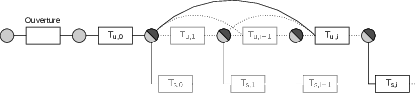
\includegraphics{chapters/img/eltoo-offchain-protocol.png}

}

\caption{Overview of the Eltoo protocol.}

\end{figure}%

An additional transaction is added to the chain to prevent the
expiration delay of settlement transactions \(T_{s,i}\) from being
reached and them being broadcast on-chain. This transaction simply sends
the funds to a regular multisignature account and is signed and
broadcast after the signing of the initial update and settlement
transactions (\(T_{u,0}\) and \(T_{s,0}\)). The expiration delay only
begins when transaction \(T_{u,0}\) is broadcast.

This mechanism allows for a simple protocol for updating the channel,
less constraining for nodes, without a penalty mechanism, and without
needing to decide fees in advance. This ease of implementation could
facilitate the creation of more complex contracts on Lightning, such as
payment channels with three or more participants. Moreover, their
implementation does not need to replace that of Poon-Dryja channels;
both models can coexist within a single network of payment channels.

Floating transactions are implemented using SIGHASH\_ANYPREVOUT. Thus,
the realization of Eltoo relies on the integration of BIP-118 into
Bitcoin.

\section*{Inscription of Arbitrary
Data}\label{inscription-of-arbitrary-data}
\addcontentsline{toc}{section}{Inscription of Arbitrary Data}

\markright{Inscription of Arbitrary Data}

Bitcoin allows the inscription of non-financial data on the chain---that
is, data not necessary for locking and unlocking funds and interpreted
outside the protocol. Even with all possible restrictions, it's
impossible to prevent the inscription of such data, although it can be
made more costly.

The main chain of Bitcoin is widely shared around the world and will be
preserved by humanity, at least as a historical relic, suggesting that
what is stored there will be kept for a very long time. This
characteristic encourages people to include things that matter to them.
It's human nature to seek to leave traces of our passage on Earth, and
writing on a supposedly immutable ledger is one way to do it.

Various methods of inscription exist, each with its own qualities and
drawbacks. These have evolved over the years as this usage became more
prevalent.

On one hand, arbitrary data can be written by miners within the coinbase
transaction input, specifically in the unlocking script. This field is
conceptually superfluous---the coinbase doesn't refer to any existing
output---and can thus be used at discretion. This is the method Satoshi
Nakamoto used to inscribe the now-famous headline from the January 3,
2009, issue of \emph{The Times} in the genesis block:

\emph{``The Times 03/Jan/2009 Chancellor on brink of second bailout for
banks''}

Other blocks contain notable messages. The exodus block of BCH (height
478,559) included a welcome message for Shuya Yang, the daughter of the
CEO of the ViaBTC mining pool. The block preceding the third halving on
BTC in 2020 (height 629,999) included the headline from a \emph{New York
Times} article dated April 9 announcing the Federal Reserve's record
liquidity injection of \$2.3 trillion in response to the COVID-19
crisis: ``\emph{NYTimes 09/Apr/2020 With \$2.3T Injection, Fed's Plan
Far Exceeds 2008 Rescue}.''

The coinbase unlocking script can be used to write other data as well.
This includes the extra nonce (the criterion that helped identify
Satoshi's bitcoins). It's also how mining pools signal themselves
through this field; for example, the coinbase of block 751,005 contains
the string \emph{poolin.com}, indicating that it was likely validated by
the Chinese pool Poolin.

On the other hand, users can include arbitrary data within their
transactions and pay the corresponding fees. Several methods have been
used for this.

Before 2014, these inscriptions were most often made by storing data in
locking scripts, for example, using the \texttt{OP\_DROP} stack
instruction\footnote{Transaction
  c0b2cf75b47d1e7f48cdb4287109ff1dd5bcf146d5f77a9e8784c0c9c0ef02ad,
  confirmed on December 13, 2012, contains the string
  \emph{TheCakeIsALie\textbackslash n} in reference to the video game
  \emph{Portal}.}. Another common practice was inscribing data in
P2PKH-type outputs, which were then rendered unspendable. This method
was extremely costly due to the transaction structure (requiring
inscription in the outputs) and the need to send non-zero amounts in
outputs. It was also detrimental to the system as a whole because it
bloated the entire UTXO set.

After 2014, a more efficient way to store data was authorized through
the standardization of the NULLDATA scheme based on the
\texttt{OP\_RETURN} instruction. This change allowed for the creation of
``provably prunable outputs, to avoid data storage schemes {[}\ldots{]}
that were storing arbitrary data, such as images, as forever unspendable
transaction outputs, thereby bloating Bitcoin's UTXO
database\footnote{Bitcoin Core, \emph{Bitcoin Core version 0.9.0
  released}, March 19, 2014:
  \url{https://bitcoin.org/en/release/v0.9.0\#opreturn-and-data-in-the-block-chain}.}.''
It also limited the wastage of funds by allowing the creation of a
0-satoshi output. This scheme quickly became the most popular way to
publish information on the chain.

Furthermore, it's possible to store data within transaction inputs or
associated witnesses when spending P2SH, P2WSH, or P2TR outputs. This
writing can occur in the redeem scripts or in the unlocking elements.
This method has the advantage of not overloading the entire UTXO set.
For users, for inputs where SegWit applies, it has the benefit of
reducing the cost of arbitrary data inscribed in the transaction by
four.

These different methods have been used to inscribe various items on the
chain, including cryptographic hashes, text, and images\footnote{Ken
  Shirriff, \emph{Hidden surprises in the Bitcoin blockchain and how
  they are stored: Nelson Mandela, Wikileaks, photos, and Python
  software}, February 16, 2014:
  \url{https://www.righto.com/2014/02/ascii-bernanke-wikileaks-photographs.html}.}.

First, one can inscribe a hash, with the inscription serving as a
timestamp. This involves inscribing the hash of a file on the chain as
proof of existence. This idea was put forward in February 2009 by Hal
Finney in an email to the Bitcoin mailing list. He suggested that ``the
Bitcoin block chain would be perfect'' to ``prove that a certain
document existed at a certain time in the past\footnote{Hal Finney,
  \emph{Re: {[}bitcoin-list{]} Bitcoin v0.1.5 released}, February 27,
  2009, 20:00:12 UTC, archived:
  \url{https://web.archive.org/web/20131016004925/http://sourceforge.net/p/bitcoin/mailman/bitcoin-list/?viewmonth=200902}.},''
a view approved by Satoshi. In essence, this practice allows one to
demonstrate knowledge of information before its publication and thus
indirectly claim probable authorship. This type of use has notably been
implemented by the French company Woleet.

This possibility can also be exploited by decentralized file hosting
systems like IPFS (InterPlanetary File System), which uses file hashes
to identify them and allows their storage by a peer-to-peer network of
users. It's thus possible to associate text written on the blockchain
with images or videos hosted in a decentralized manner.

Next, one can inscribe text, usually encoded in ASCII/UTF-8. For
example, the phrase ``Beauty will save the world.'' was inscribed on the
BTC chain on August 10, 2022, in transaction
08e5ce0783ab6d5534e234136df02e0e240f76108eb6af04b8b624646b66f5eb.
Inscribing texts also allows for drawing images in ASCII art. This is
the case with the tribute to Len Sassaman (see
Figure~\hyperref[fig:sassaman-tribute]{13.6}), who passed away in July
2011. It was inscribed on the chain by developers Dan Kaminsky and
Travis Goodspeed in P2PKH outputs and notably contains a representation
of former Fed Chairman Ben Bernanke.

Tribute to Len Sassaman (ASCII art).

Finally, one can include an image, which can be encoded in multiple
formats, notably JPEG or PNG. For example, a Bitcoin logo inscribed on
May 13, 2011, can be found. A tribute to Nelson Mandela along with a
photo was published on December 7, 2013, a few days after his death. In
2022, the lack of standard restrictions on Taproot script size allowed
for voluminous inscriptions in a much more transparent and direct way.
This notably enabled the inscription of the Taproot Wizards image, which
was nearly 4~MB in size (see
Figure~\hyperref[fig:taproot-wizards]{13.7}).

\begin{figure}

{\centering 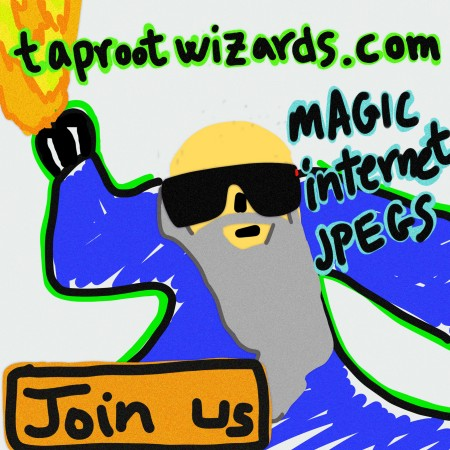
\includegraphics{chapters/img/taproot-wizards-small-0301e0480b374b32851a9462db29dc19fe830a7f7d7a88b81612b9d42099c0aei0.jpg}

}

\caption{Image (reduced) of the Taproot Wizards.}

\end{figure}%

In general, any file format can be stored on the chain through multiple
transactions: a document, a book, a video, a game, etc. However, this
use is not always appropriate. Inscription requires paying fees,
sometimes high, and the BTC blockchain isn't really designed to store
large amounts of data. Publishing these files on IPFS or on a local
server is generally more suitable.

Note that the Bitcoin SV community focused on data storage, considering
its ledger as a ``universal source of truth\footnote{CoinGeek,
  \emph{Jerry Chan: Bitcoin's value is as a universal source of truth},
  July 17, 2019:
  \url{https://coingeek.com/jerry-chan-bitcoins-value-is-as-a-universal-source-of-truth-video/}.}.''
Consequently, a significant volume of weather data, inscribed since
2019, can be found on its chain. This has made the BSV network extremely
centralized in terms of both mining and commerce, which questions the
primary utility of recording information on a blockchain: immutability.

\section*{Metaprotocols}\label{metaprotocols}
\addcontentsline{toc}{section}{Metaprotocols}

\markright{Metaprotocols}

Metaprotocols are protocols that leverage the base protocol to function.
They utilize the inscription of arbitrary data on the chain to include
instructions interpreted by specific software implementations. They are
characterized by being more extensive than the base protocol.

This is not a novel idea. From Bitcoin's early years, some individuals
sought to exploit it more deeply, using it in ways beyond a simple value
transfer instrument. This initial movement, aiming to add
functionalities to Bitcoin in this manner, was termed ``Bitcoin 2.0.''
It eventually led to the development of Ethereum starting in 2013.

The first type of metaprotocol developed was the concept of
\emph{colored coins}, which involves marking coins (UTXOs) by the
additional inscription of data, as illustrated in
Figure~\hyperref[fig:colored-coin]{13.8}. Each type of token created is
linked to an identifier, which can be likened to a color, hence the name
of this approach. The idea was presented in 2012 by Yoni Assia and Meni
Rosenfeld\footnote{Yoni Assia, \emph{bitcoin 2.X (aka Colored Bitcoin)
  -- initial specs}, March 27, 2012:
  \url{https://yoniassia.com/coloredbitcoin/}; Meni Rosenfeld,
  \emph{Overview of Colored Coins}, December 4, 2012:
  \url{https://bitcoil.co.il/BitcoinX.pdf}.}.

\begin{figure}

{\centering 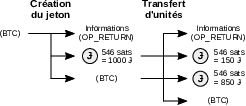
\includegraphics{chapters/img/colored-coin.png}

}

\caption{Creation and transfer of a token issued as a colored coin.}

\end{figure}%

The implementation of this concept was carried out at the end of 2012
through the ChromaWallet. However, it only gained momentum from 2014,
with the emergence of Coinprism's Open Assets, Coin Sciences' CoinSpark
assets, and Colu's Colored Coins. These uses have since fallen into
disuse, although the procedure has been employed sporadically over the
years, such as with Bisq's BSQ token created in 2018 as the basis of its
DAO. An attempt at revival was also made on Bitcoin Cash with SLP
tokens, without significant success.

Beyond colored coins, more advanced protocols existed that managed their
own unit of account. These were primarily Mastercoin, later renamed Omni
in March 2015, and Counterparty.

The first advanced metaprotocol was Mastercoin, whose white paper,
titled ``\emph{The Second Bitcoin Whitepaper}'', was published on
January 6, 2012, by J.R. Willett\footnote{J.R. Willett, \emph{The Second
  Bitcoin Whitepaper}, January 6, 2012, archived:
  \url{https://cryptochainuni.com/wp-content/uploads/Mastercoin-2nd-Bitcoin-Whitepaper.pdf}.}.
It was a protocol allowing users to create their own currencies, called
``user currencies.'' Mastercoin was based on a unit of account noted as
MSC, which was the subject of a one-month presale in July-August
2013\footnote{All bitcoins sent to address
  1EXoDusjGwvnjZUyKkxZ4UHEf77z6A5S4P were converted into MSC at a rate
  of 100~MSC at the beginning, decreasing over the weeks.}. It was the
first Initial Coin Offering (ICO) in history, raising 5,120~BTC, over
\$500,000 at that time.

Perhaps the greatest success of this protocol was the creation of the
first stablecoin, Tether USD, initially issued under the name Realcoin
in October 2014. Mastercoin/Omni was long the only way to own and
transfer USDT before the token was massively issued on other chains like
Ethereum and Tron.

The second advanced metaprotocol was Counterparty, launched in January
2014. This platform also relied on a native token, XCP, which served as
its fuel and was created by burning bitcoins during its first month of
existence\footnote{All bitcoins sent to address
  1CounterpartyXXXXXXXXXXXXXXXUWLpVr between January 2 and February 3,
  2014, were converted into XCP at a rate that varied between 1,000 and
  1,500~XCP per~BTC.}. Approximately 2,140 bitcoins were made unusable
to give life to over 2.6 million XCP, still in circulation today.
Counterparty aimed to be more flexible than Mastercoin by enabling the
implementation of autonomous contracts, particularly to create tokens
and host decentralized exchange platforms called ``dispensers.''

In particular, Counterparty was the first platform to offer the
management of non-fungible tokens (NFTs). This implemented an old idea,
notably highlighted by Hal Finney in 1993 on the cypherpunk mailing list
as ``cryptographic trading cards\footnote{Hal Finney, \emph{Crypto
  trading cards.}, January 17, 1993, 18:48:02 UTC:
  \url{https://cypherpunks.venona.com/date/1993/01/msg00152.html}.}.''
Counterparty hosted numerous such collections, like the \emph{Spells of
Genesis} and SaruTobi playing cards created in 2015, or the Rare Pepes
issued between 2016 and 2018.

In 2018, the emergence of Bitcoin Cash motivated the creation of a
social media platform whose data would be entirely stored on-chain, as
BCH developers were more liberal in this regard. The protocol was called
Memo and involved publishing short messages publicly visible under a
defined profile, following other users, and liking and replying to their
messages. The idea was to achieve a sort of censorship-resistant social
network but suffered from the need to pay fees for each action.

All these protocols lost their appeal until the emergence of the
Ordinals protocol, launched in January 2023. This metaprotocol allowed
the creation and management of ``digital artifacts,'' i.e., NFTs whose
full data is immutably stored on a censorship-resistant chain. Ordinals
relied on an ``ordinal theory'' allowing for the tracking and transfer
of satoshis linked to an inscription, such as text, images, or other
data. In particular, Ordinals was used to emulate the ownership and
transfer of fungible tokens, dubbed ``BRC-20,'' whose speculative
success caused network congestion leading to historically high
transaction fees. The success of Ordinals also inspired the creation of
the STAMPS protocol, based on Counterparty for artifact tracking and
storing their data in P2MS outputs.

All these practices sparked debates. Bitcoin was presented as a model of
digital currency, and it seemed counterproductive to turn it into a data
preservation protocol unrelated to bitcoin transfers. As early as
December 2010, Jeff Garzik opposed using the chain for generalized
storage\footnote{Jeff Garzik, \emph{Resist the urge to use block chain
  for generalized storage}, December 7, 2010, 22:04:54 UTC:
  \url{https://bitcointalk.org/index.php?topic=2129.msg27884\#msg27884}.}.
Later, in 2014, similar disputes arose concerning
Counterparty\footnote{BitMEX Research, \emph{The OP\_Return Wars of
  2014---Dapps Vs Bitcoin Transactions}, July 12, 2022:
  \url{https://blog.bitmex.com/dapps-or-only-bitcoin-transactions-the-2014-debate/}.}.
In 2023, the same discord occurred following the success of
Ordinals\footnote{pourteaux, \emph{Illegitimate bitcoin transactions},
  January 25, 2023:
  \url{https://read.pourteaux.xyz/p/illegitimate-bitcoin-transactions}.}.

These metaprotocols have two major flaws. The first is that verifying
their rules depends on a small subset of network nodes. Indeed, managing
such an overlay protocol requires additional resources, particularly for
indexing in the case of colored coins. Consequently, few people deploy a
complete implementation, significantly centralizing the protocol and
making it susceptible to alteration by an adversary aiming to censor it.

The second flaw concerns their sometimes very high usage fees,
especially if the network's transactional capacity limit is reached.
Transactions implementing these solutions are necessarily larger than
normal transactions, leading to higher fees. They are therefore more
easily excluded by the fee increases resulting from network congestion.

For these reasons, those who worked on these solutions quickly moved
away from them, preferring to turn to alternative platforms like NXT and
especially Ethereum. Vitalik Buterin himself was interested in colored
coins and Mastercoin in 2013 before starting to build what would become
Ethereum\footnote{Yoni Assia, Vitalik Buterin, Meni Rosenfeld, Rotem
  Lev, \emph{Colored Coins whitepaper}, 2013:
  \url{http://www.ma.senac.br/wp-content/uploads/2018/05/ColoredCoinswhitepaper-DigitalAssets.pdf};
  Vitalik Buterin, \emph{A Prehistory of the Ethereum Protocol},
  September 14, 2017:
  \url{https://vitalik.ca/general/2017/09/14/prehistory.html}.}. It's
also for these reasons that less costly solutions---overlays using the
chain as a settlement mechanism rather than as a place to record all
operations---are now favored for such purposes, like RGB or Taproot
Assets.

\section*{Off-Chain Contracts}\label{off-chain-contracts}
\addcontentsline{toc}{section}{Off-Chain Contracts}

\markright{Off-Chain Contracts}

Cryptography allows for the deployment of contracts without them having
to be inscribed on-chain. This capability was facilitated by the
Schnorr-Taproot upgrade, often simply called ``Taproot,'' which occurred
on BTC on November 14, 2021. It included two major elements: the Schnorr
signature scheme and the Taproot contract programming method. These
features were integrated as a soft fork within the standard P2TR scheme
corresponding to SegWit's version~1.

The Schnorr scheme implemented is a derivation of the authentication
protocol described in 1989 by Claus-Peter Schnorr. It is an alternative
to ECDSA, based on the same elliptic curve (secp256k1), and allows
transactions to be signed using the same key pairs.

Compared to ECDSA, the Schnorr signature scheme has several advantages.
First, it produces smaller signatures. Second, the signatures produced
are non-malleable, as the procedure doesn't involve random numbers.
Third, and most importantly, it exhibits a property of linearity,
enabling functionalities like batch verification and key aggregation.

The Schnorr scheme is superior to ECDSA and existed in 2008, but Satoshi
Nakamoto chose not to use it. This choice can be explained by the
algorithm being patented in the United States until February 2008,
meaning there was no standardized implementation. Bitcoin's software
used OpenSSL, which didn't include this type of algorithm.

The Schnorr scheme allows the deployment of \emph{Scriptless Scripts},
contracts ``without script'' that are executed off-chain and applied
within the signatures. The concept was theorized in 2017 by Andrew
Poelstra\footnote{Andrew Poelstra, \emph{Using the Chain for what Chains
  are Good For} (video), Scaling Bitcoin IV, November 5, 2017:
  \url{https://www.youtube.com/watch?v=3pd6xHjLbhs&t=5755s}; Aaron van
  Wirdum, ``\emph{Scriptless Scripts: How Bitcoin Can Support Smart
  Contracts Without Smart Contracts}'', \emph{Bitcoin Magazine},
  November 27, 2017:
  \url{https://bitcoinmagazine.com/technical/scriptless-scripts-how-bitcoin-can-support-smart-contracts-without-smart-contracts}.}.
It is found in examples like the MuSig2 multiparty signature scheme,
Adaptor Signatures, or Discreet Log Contracts.

Moreover, the Schnorr scheme greatly facilitates the implementation of
Taproot (BIP-341), which was integrated into the protocol
simultaneously. Taproot (literally meaning ``taproot'' in English) is a
method for programming autonomous contracts that anchors the clauses of
a contract within a Merkle tree and hides this tree under an aggregated
public key belonging to its participants. It allows the contract to be
published only in case of dispute and, even then, only the executed
conditions are revealed. The scripts used in Taproot employ a
programming language called Tapscript (BIP-342), based on Bitcoin's
classic script language.

Taproot relies on a hash tree called a MAST\footnote{The acronym MAST
  originally stands for \emph{Merklized Abstract Syntax Trees},
  referring to data structures described in BIP-114. In Taproot, these
  aren't truly abstract syntax trees, but the term remains used. The
  hash trees in Taproot can be called \emph{Merklized Alternative Script
  Trees} by retroacronymy. See Anthony Towns, \emph{{[}bitcoin-dev{]}
  Safer sighashes and more granular SIGHASH\_NOINPUT}, November 23,
  2018, 05:03:30 UTC:
  \url{https://lists.linuxfoundation.org/pipermail/bitcoin-dev/2018-November/016500.html}.},
whose leaves are the clauses of the contract---that is, the spending
conditions. During MAST execution, the concerned participants need only
reveal the applied clause and provide the hashes related to the other
clauses (Merkle path), as shown in
Figure~\hyperref[fig:taproot-mast]{13.9}. The other spending conditions
are thus not revealed.

\begin{figure}

{\centering 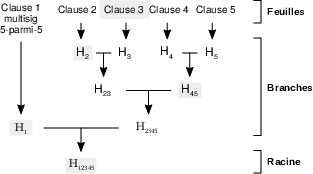
\includegraphics{chapters/img/taproot-mast.png}

}

\caption{MAST involving the clauses of a contract.}

\end{figure}%

The implementation of such MASTs within Bitcoin had been proposed in the
past, either in the form of a new SegWit version (BIP-114) or a new
opcode called \texttt{OP\_MERKLEBRANCHVERIFY} (BIP-116, BIP-117).
However, Taproot constituted a superior proposal by allowing the MAST's
existence itself to remain hidden.

Indeed, Taproot includes an integrated cooperative spending condition.
The internal aggregated public key is slightly modified (\emph{tweaked})
using the MAST root to account for it. The resulting key is the one
recorded in the coin's locking script, making it indistinguishable from
other P2TR outputs. Similarly, the aggregated signature cannot be
distinguished from a classic signature. Thus, participants can spend the
funds amicably while ensuring that any dispute will lead to on-chain
settlement.

An alternative to Taproot is RGB, a system of off-chain autonomous
contracts built both on top of Bitcoin and Lightning. The name comes
from the RGB standard (\emph{Red Green Blue}), which is used to define a
color, directly referencing colored coins, as RGB was originally
conceived as ``a better version of colored coins\footnote{RGB FAQ,
  \emph{What does `RGB' stand for?}, December 14, 2020:
  \url{https://www.rgbfaq.com/faq/what-does-rgb-stand-for}.}.'' However,
while RGB indeed allows the issuance and management of tokens, this
functionality is far from the only one.

RGB is based on two technical primitives conceptualized in 2016 by
developer Peter Todd: client-side validation and single-use seals. This
allows the management of an independent state where double-spending is
prevented by these seals. After research by Giacomo Zucco and the BHB
Network, RGB is currently developed by the LNP/BP Standards Association.

Implementing contracts off-chain is thus possible on Bitcoin, bringing
two main benefits. First, it reduces fee payments by having a minimal
on-chain footprint. Second, it improves the privacy of participants.
This potential positions them to play a significant role in the long
term.

\section*{A Programmable Currency}\label{a-programmable-currency}
\addcontentsline{toc}{section}{A Programmable Currency}

\markright{A Programmable Currency}

The programmable aspect of Bitcoin is often overlooked. It's not
directly presented in the white paper, even though Satoshi Nakamoto had
already developed it by then. However, it's very useful and constitutes
one of Bitcoin's essential facets.

Currency programmability can be used for control, as illustrated by the
CBDC projects emerging worldwide. But it can also greatly enhance
individual freedom. This modular aspect allows people who don't know
each other to exchange value in the most secure way possible or, as Tim
May expressed in his \emph{Crypto Anarchist Manifesto} of 1988, to ``do
business and negotiate contracts electronically with strangers, without
ever knowing the True Name, or legal identity, of the
other\footnote{Timothy C. May, \emph{The Crypto Anarchist Manifesto},
  November 22, 1992, 20:11:24 UTC:
  \url{https://cypherpunks.venona.com/date/1992/11/msg00204.html}.}.''

Autonomous contracts form the cornerstone of financial relations in
cyberspace. Even the Monero community, which had particularly restricted
this aspect for privacy reasons, retraced its steps by integrating
multisignature functionality into the protocol, notably to allow atomic
swaps. A truly free currency must be freely programmable.

\bookmarksetup{startatroot}

\chapter{Scaling Up}\label{ch:scalability}

\phantomsection\label{enotezch:14}{}

{S}\textsc{c}alability, a direct borrowing from the English term
``scalability,'' also known as extensibility, refers to a system's
capacity to scale up---that is, to continue functioning equivalently as
the number of users increases. In a centrally managed system, this
capability is ensured by adding computing hardware, either by increasing
the computational power of the existing infrastructure (vertical
scaling) or by multiplying instances of the infrastructure to share
request processing (horizontal scaling). Consequently, scalability
depends on the forecasting level of the entity managing the system.

In the case of a distributed system, which behaves differently,
scalability refers to something more complex. Adding hardware is not
sufficient; the system's properties must also remain consistent as
activity increases. In Bitcoin's case, this problem is particularly
difficult because any increase in load permanently affects the network
nodes due to the need to share the entire blockchain. Essentially, the
system does not scale---or scales very little.

This scalability issue in Bitcoin has been a major concern within the
community, to the point of provoking an open conflict between 2015 and
2017: the infamous block wars described in
Chapter~\hyperref[ch:clivages]{2}. Some believed that increasing the
block size would suffice to handle demand without altering supply, while
others imagined that overlay solutions like the Lightning Network would
be effective enough to process all transfers. This chapter aims to
provide an overview of the situation and propose a third way.

\section*{The System's Lack of
Scalability}\label{the-system-s-lack-of-scalability}
\addcontentsline{toc}{section}{The System's Lack of Scalability}

\markright{The System's Lack of Scalability}

Bitcoin's original design is based on a simple principle: obtaining and
verifying all transactions to ensure there is no double spending. As
Satoshi Nakamoto wrote in the white paper, ``the only way to confirm the
absence of a transaction is to be aware of all
transactions\footnote{Satoshi Nakamoto, \emph{Bitcoin: A Peer-to-Peer
  Electronic Cash System}, October~31, 2008.}.'' Therefore, to achieve
maximum security, each node must, in principle, maintain a complete
version of the blockchain.

From the outset, this particular functioning naturally raised the
question of the system's scalability. When Satoshi Nakamoto presented
his discovery on the Metzdowd.com cryptography mailing list on October
31, 2008, the first response he received addressed this problem. This
response came from former cypherpunk James A. Donald on November 2, who
wrote:

``We very, very much need such a system, but as I understand your
proposal, it does not seem to scale to the required size.

For transferable proof of work tokens to have value, they must have
monetary value. To have monetary value, they must be transferred within
a very large network---as, for example, a file sharing network like
Bittorrent.

To detect and reject a double-spending event in a timely manner, one
must have most past transactions of the coins involved in the
transaction, which, if implemented naively, requires each peer to have
most past transactions, or most past transactions that have recently
occurred. If hundreds of millions of people are doing transactions, that
is a lot of bandwidth---each must know all transactions or a substantial
fraction thereof\footnote{James A. Donald, \emph{Re: Bitcoin P2P e-cash
  paper}, November 2, 2008, 23:46:23 UTC:
  \url{https://www.metzdowd.com/pipermail/cryptography/2008-November/014814.html}.}.''

By this, James A. Donald highlighted Bitcoin's lack of scalability. For
any given system, an increase in transaction volume raises the number of
transactions to obtain and process. This increase makes operating a node
more difficult, potentially affecting the network's decentralization
and, consequently, security. Therefore, there is always a trade-off
between the system's utility and its security---or, more precisely,
between ease of transaction and ease of verification.

This trade-off generally manifests as a limit on transaction capacity,
described by the consensus rules (explicit limit) or, more rarely, by
network rules (implicit limit). The transaction capacity limit was
originally defined as a maximum block size, prohibiting miners from
creating blocks larger than a certain size. In the prototype, this size
was implicitly defined by the maximum size of protocol transmission
messages, that is, 32~MB. Then, an explicit limit of 1 megabyte (1~MB)
was added by Satoshi Nakamoto in September 2010 through the constant
MAX\_BLOCK\_SIZE, without any public announcement from him, to prevent
denial-of-service attacks. This size corresponded, for a network running
at full capacity, to a theoretical volume of 4.5 standard transactions
per second, which in practice amounted to about 3 transactions per
second.

With the integration of SegWit into the main version of Bitcoin in
August 2017, this limitation became a weight limit of blocks. This new
metric gave greater importance to the base size compared to the witness
size in the calculation of the block's measure, also modifying how
miners counted to add transactions to the block. This change was an
effective increase in the protocol's transaction capacity, raising the
allowed transaction volume to 8 transactions per second theoretically,
and to 4.5 transactions per second in practice.

The existence of a transaction capacity limit inevitably creates
scarcity of block space. If it is fixed, it makes the supply inherently
inelastic. Thus, strong demand for block space leads, through an auction
effect, to an increase in the price for inclusion---that is, transaction
fees. The fee market is stimulated by this rigid limit instead of
remaining at its natural level, namely the default inclusion cost for
miners.

Through its effect on fee levels, the limit creates a utility
floor---that is, a value level below which transfer and holding are not
considered profitable by users. Indeed, miners are led to reject
transactions that do not pay a sufficient fee rate relative to their
size. Consequently, the utility of a transaction may be deemed
insufficient by its author concerning the average fee level of the
chain, in which case it does not occur. If someone wants to buy a coffee
for \$2 in BTC but the usual fees are \$1, they will quickly move on.
Generally, use cases requiring ``low'' fees are driven off the chain, as
in the case of the gambling service SatoshiDICE, which had to cease its
activities on BTC in 2017 following the increase in fees.

The transaction capacity limit has the virtue of ensuring that the cost
of operating a node remains low. It thus impacts the network's
\emph{potential} decentralization. Indeed, unlike mining hardware, the
cost related to verification is not offset by a proportional income, so
it affects everyone equally. The least equipped node operators cannot
keep up, which can affect the network's ability to decentralize
\emph{effectively}.

The influence on potential decentralization affects both mining and
commerce by preventing smaller actors from engaging in these activities
at their scale. The centralization of mining increases the risk of
censorship, while the centralization of commerce raises the risk of
protocol alteration, and thus inflation risk. This is why the
transaction capacity limit plays a major role in the security model: the
lower this limit, the greater the system's \emph{potential} security.

The transaction capacity limit is subjectively determined by merchants,
based on their \emph{perception of the threat} and their \emph{personal
use} of the chain. There is no ideal block size limit; there are only
human beings calculating risk relative to a potential reward. One might
attempt to establish an average to estimate a limit corresponding to a
given usage, but such an estimate would be at best imperfect.

Through its effect on decentralization, the limit creates a utility
ceiling---that is, a value level above which transfer and holding are
considered too risky for the system's effective security. Indeed, since
no security is absolute, transferring and holding a certain value may no
longer sufficiently benefit from the network's protection. For example,
receiving or storing the equivalent of several million dollars on the
Bitcoin SV chain is, to say the least, imprudent.

The utility floor (induced by the limit's negative impact on block
space) and the utility ceiling (induced by the limit's positive impact
on security) have the effect of bounding a range of values outside which
transfer and holding are no longer relevant\footnote{See Eric Voskuil,
  ``Utility Threshold Property,'' in \emph{Cryptoeconomics: Fundamental
  Principles of Bitcoin}, Amazon KDP, 2022, pp.~317--318.}. It is the
existence of this range of values that leads to the emergence of
substitutes for a given system.

The arrival of new users and the subsequent increase in demand for block
space raise the utility floor. Any scaling up of the system modifies its
characteristics. Therefore, any Bitcoin system is essentially
non-scalable, in the primary sense of the term. However, there are
methods to circumvent this lack of scalability.

\section*{Improving Base Efficiency}\label{improving-base-efficiency}
\addcontentsline{toc}{section}{Improving Base Efficiency}

\markright{Improving Base Efficiency}

The first proposal regarding scaling up was to gradually increase the
block size limit to accompany the rise in activity\footnote{Among the
  alternative versions of Bitcoin, the path of progressively increasing
  the block size limit was chosen by Bitcoin Cash, which plans to
  integrate an algorithm to manage this increase automatically. See
  bitcoincashautist, \emph{CHIP-2023-04: Adaptive Blocksize Limit
  Algorithm for Bitcoin Cash}, September~2, 2023:
  \url{https://gitlab.com/0353F40E/ebaa/-/blob/f4edacd134103a7e232740463a5f26379bf90f18/README.md}.}.
This was the solution supported by Satoshi Nakamoto, as evidenced by his
first reaction to James A. Donald's response on November 3, 2008:

``Bandwidth might not be as prohibitive as you think. A typical
transaction is about 400 bytes (ECC is nice and compact). Transactions
need to be broadcast twice, so let's say 1~KB per transaction. Visa
processed 37 billion transactions in FY2008, so that's 100 million
transactions per day. That many transactions would take 100~GB of
bandwidth, or the size of 12 DVDs or about 2 HD quality movies, or about
\$18 worth of bandwidth at current prices. If the network were to get
that big, it would take several years, and by then, sending two HD
movies over the Internet probably won't seem like a big
deal\footnote{Satoshi Nakamoto, \emph{Re: Bitcoin P2P e-cash paper},
  November~3, 2008, 01:37:43 UTC:
  \url{https://www.metzdowd.com/pipermail/cryptography/2008-November/014815.html}.}.''

However, Satoshi's vision was far too optimistic. On one hand, he did
not see mining centralization as an existential problem, predicting from
the start that the network's computing power would rely on ``server
farms with specialized hardware.'' On the other hand, he thought that
Simplified Payment Verification (SPV) would suffice, not accounting for
its unreliability and lack of confidentiality, nor its inability to
exert power over determining consensus rules. Satoshi's plan was
therefore fallible, though not entirely misguided.

Operating a node depends on a number of burdens. The main ones are hard
disk storage (HDD) for the history (blockchain), flash memory storage
(SSD) for the state (UTXO set), random access memory (RAM) storage for
the unconfirmed transaction pool (mempool) and orphan block pool,
maintaining bandwidth (usually expressed in Mbps) sufficient to receive
and send blocks and transactions, and CPU computation for data
verification, notably signatures. Reducing the cost of running a node
thus involves reducing one of these burdens.

Even if naive increases to the block size limit are not in themselves a
scalability method, they can be offset by technical progress from
software, hardware, or algorithmic optimization. Firstly, software
performance (for a given set of consensus rules) can be improved, and
this is indeed one of the basic tasks of the Bitcoin Core
team\footnote{See, for example, Jameson Lopp's article on Bitcoin Core
  performance evolution, in which he describes how the first
  synchronization on his machine has improved over the years. ---
  Jameson Lopp, \emph{Bitcoin Core Performance Evolution}, March~5,
  2022: \url{https://blog.lopp.net/bitcoin-core-performance-evolution/}.}.
Secondly, computer hardware can be made more efficient, with certain
components gradually becoming less expensive (Moore's Law\footnote{Moore's
  Law is a conjecture stated by Gordon E. Moore in 1965, which posited
  that the complexity of semiconductors doubled every year. This law was
  cited by Satoshi Nakamoto in the white paper, who wrote: ``Moore's Law
  predicts current growth of 1.2~GB per year, so storage should not be a
  problem even if the block headers must be kept in memory.'' ---
  Satoshi Nakamoto, \emph{Bitcoin: A Peer-to-Peer Electronic Cash
  System}, October~31, 2008.}). Thirdly, the protocol itself can be
improved at the algorithmic level, through the discovery and adoption of
new, more efficient techniques: for example, the Schnorr signature
algorithm produces more compact signatures than ECDSA (40~bytes instead
of 72), or bulletproofs make the range proofs of Confidential
Transactions much less voluminous.

Beyond these optimizations, there is no way to increase the transaction
volume of the chain without compromising the Bitcoin model. The solution
is to modify the system's behavior in such a way that it does not overly
affect the security model. Several factors can thus be optimized,
including the size of the chain to keep, the Initial Block Download
(IBD), and the size of the UTXO set.

First, one can choose to delete the oldest blocks once they have been
verified. One simply keeps the chain of headers, the network state, and
the most recent blocks to be able to rejoin consensus in the event of a
deep reorganization. This method is called pruning.

But this method does not alleviate the burden of the IBD, that is, the
process of downloading and verifying the blockchain up to its current
height. To address this, various more or less risky techniques can be
employed. The first is signature validity assumption, based on the
\texttt{assumevalid} parameter, introduced in Bitcoin Core in
2017\footnote{Bitcoin Core, \emph{Bitcoin Core 0.14.0}, March~8, 2017:
  \url{https://bitcoincore.org/en/2017/03/08/release-0.14.0/\#assumed-valid-blocks}.},
which involves skipping signature verification up to a given block hash,
saving a lot of time during initial synchronization. This method is not
a checkpoint (it does not require the block to exist), and the risk it
poses is minimal. The second technique is AssumeUTXO, proposed in 2019
by James O'Beirne and still in development\footnote{James O'Beirne,
  \emph{AssumeUTXO Proposal}, April~24, 2019:
  \url{https://github.com/jamesob/assumeutxo-docs/tree/2019-04-proposal/proposal}.},
which involves assuming valid a given UTXO set (identified by its hash)
at a determined block height: the node operator downloads the UTXO
snapshot from a third party and begins initial synchronization from
there, deferring (or entirely ignoring) the download and verification of
previous blocks. This method presents a verification defect (at least
temporarily), exposing the operator to deception, but the risk is
considered acceptable. There is also a third, more radical technique:
UTXO commitments, which is a soft fork requiring miners to add the UTXO
set hash to the block\footnote{Mark Friedenbach, \emph{{[}soft fork{]}
  Block v3: miner commitments with compact proofs}, March~28, 2014:
  \url{https://github.com/bitcoin/bitcoin/pull/3977}; Pieter Wuille,
  \emph{{[}bitcoin-dev{]} Rolling UTXO set hashes}, May~15, 2017,
  20:01:14 UTC:
  \url{https://lists.linuxfoundation.org/pipermail/bitcoin-dev/2017-May/014337.html}.};
this commitment would allow a much more reliable source for downloading
the snapshot from which to begin synchronization.

Then, beyond the IBD, there remains the problem of the UTXO set size,
which is one of the most important limiting factors. The first idea to
reduce this size is a proposal by Cory Fields called UHS (for UTXO Hash
Set), which involves storing only the hashes of individual
UTXOs\footnote{Cory Fields, \emph{UHS: Full-node security without
  maintaining a full UTXO set}, May~16, 2018, 16:36:35 UTC:
  \url{https://lists.linuxfoundation.org/pipermail/bitcoin-dev/2018-May/015967.html}.}.
The second idea is to use cryptographic accumulators, as Thaddeus Dryja
did with his proposal named Utreexo, which involves grouping UTXOs into
Merkle trees to condense the set to keep in memory, at the cost of a
trade-off on bandwidth\footnote{Thaddeus Dryja, \emph{Utreexo: A dynamic
  hash-based accumulator optimized for the Bitcoin UTXO set}, June~6,
  2019: \url{https://eprint.iacr.org/2019/611.pdf}.}.

Finally, one can choose to split mining and transaction verification by
separating the system's history and state into several fragments, each
supported by a (variable) part of the network. This is called sharding.
This was the idea behind using a Merkle-Patricia prefix tree (also
called a Merklix tree) vaguely considered by Bitcoin Cash developers, or
danksharding, which could be implemented in Ethereum. However, this is a
significant modification of the protocol that may never be implemented
in a version of Bitcoin.

These proposals are compromises made at the chain level, often affecting
the system in its entirety. However, it is also possible to make a
different compromise at the level of individual coins, by using banks
and, especially, overlays.

\section*{Banks and Overlays}\label{banks-and-overlays}
\addcontentsline{toc}{section}{Banks and Overlays}

\markright{Banks and Overlays}

Other proposals generally cited as alternatives to increasing block size
are solutions that avoid making all transfers on-chain by offloading
smaller ones elsewhere, these being ``bundled'' into larger
transactions. The chain is then used to settle debts, contracted
analogically (legal contract) or digitally (smart contract). This
involves considering the protocol as a settlement protocol.

The first way to do this is to reintroduce trust into the system by
contracting obligations traditionally, with what we will call here
banks. These banks can issue representative money by holding all the
funds or offer credit by keeping only fractional reserves. Using the
chain serves for settlement between banks, ensuring the transfer of
funds between their clients. This is essentially the model of free
banking promoted by George Selgin and Larry White in the 1990s.

This first conception was defended by Hal Finney, who was aware of
Selgin and White's work, as we saw in
Chapter~\hyperref[ch:cybermonnaie]{6}. On December 30, 2010, he thus
praised a free banking model based on Bitcoin:

``In fact, there is a very good reason why Bitcoin-based banks will
exist and issue their own digital currency, convertible to bitcoin.
Bitcoin itself cannot scale to have every financial transaction in the
world be broadcast to everyone and included in the blockchain. There
needs to be a secondary level of payment systems which is lighter weight
and more efficient. {[}\ldots{]} Bitcoin-based banks will solve these
problems. They can work like banks did before nationalization of money.
Different banks can have differing policies, some more aggressive, some
more conservative. {[}\ldots{]} I believe this will be the ultimate fate
of bitcoin, to be the `high-powered money' that serves as a reserve
currency for banks that issue their own digital cash. Most bitcoin
transactions will occur between banks to settle net transfers. Bitcoin
transactions by private individuals will be as rare as\ldots{} well, as
Bitcoin-based purchases are today\footnote{Hal Finney, \emph{Re: Bitcoin
  Bank}, December~30, 2010, 01:38:40
  UTC,\url{https://bitcointalk.org/index.php?topic=2500.msg34211\#msg34211}.}.''

This vision was echoed in 2018 by Saifedean Ammous in his book,
\emph{The Bitcoin Standard}, in which he argued that bitcoin's primary
role was to be a reserve currency\footnote{``Bitcoin can be seen as a
  new and emerging system of reserve currency for online transactions,
  in which online banks will issue tokens backed by bitcoin for their
  users, while keeping their reserves in bitcoins in offline storage.
  Every individual will be able to audit the intermediary's holdings in
  real time, and systems of verification and reputation will ensure that
  no inflation occurs.'' --- Saifedean Ammous, \emph{The Bitcoin
  Standard}, Wiley Publishing, 2018, p.~206.}. This thesis was later
developed by others like Nik Bhatia.

In reality, this way of diverting chain activity has materialized with
exchanges, which allowed handling the numerous buy and sell orders
related to speculation. It has also manifested through casino platforms
that grouped operations related to gambling. Finally, it has been
implemented by custodial services like Grayscale, which offered
financial institutions the possibility of including bitcoin on their
balance sheets.

However, this is not a scaling solution for Bitcoin. Bank processing is
not censorship-resistant, nor inflation-resistant, and its
generalization would ultimately lead to the total destruction of
Bitcoin's value proposition. Thus, one can reasonably assume that such a
solution can only work on a small scale, for modest amounts, insofar as
the state will not intervene, as in the case of Bitcoin Beach in El
Salvador.

The second variant of this solution is to proceed not through legal
contracts relying on trust but through smart contracts, aiming to manage
transfers off-chain. The idea is to minimize trust to make the process
viable. This was, for example, the approach behind \emph{fidelity
bonds}, proposed by Peter Todd in 2013, whose goal was to reduce the
influence of third parties while preserving clients' financial privacy
and allowing efficient auditing of banks\footnote{Peter Todd,
  \emph{Fidelity-bonded banks: decentralized, auditable, private,
  off-chain payments}, February~23, 2023, 17:49:34 UTC:
  \url{https://bitcointalk.org/index.php?topic=146307.msg1553349\#msg1553349}.}.

This approach has popularized what is generally called layering, which
involves offloading financial activity to open and decentralized
protocols, partially preserving the chain's properties. The idea is to
condense a multitude of transfers into a small number of transactions
performed on the base layer, that is, the blockchain. This terminology
comes from the decomposition into layers of the Internet protocol suite,
which is organized into multiple dependent layers, like TCP relying on
IP.

In layering, the security compromise is partial (only certain bitcoins
are concerned) and time-limited (these bitcoins can be recovered
on-chain), as opposed to the transaction capacity increase case where it
is total and persistent. It is a method consistent with the two-layer
model that Nick Szabo envisioned for bit gold, with a base layer whose
role was to guarantee the unforgeable scarcity of money, and an upper
layer that allowed effective payments.

There is thus a diversity of proposals enabling this layering by making
a more or less significant compromise. The main ones are sidechains, the
Lightning Network, and Fedimint, which we will discuss in detail later.
There are also other proposals like physical object exchange (OpenDime),
the Rumple protocol, statechains, ZK-rollups, or the Ark protocol.

\section*{Sidechains}\label{sidechains}
\addcontentsline{toc}{section}{Sidechains}

\markright{Sidechains}

Sidechains are secondary blockchains operating parallel to another
blockchain known as the ``main'' chain. They were formalized in October
2014 by Blockstream developers\footnote{Adam Back, Matt Corallo, Luke
  Dashjr, Mark Friedenbach, Gregory Maxwell, Andrew Miller, Andrew
  Poelstra, Jorge Timón, Pieter Wuille, \emph{Enabling Blockchain
  Innovations with Pegged Sidechains}, October~22, 2014:
  \url{https://blockstream.com/sidechains.pdf}.}. This technical
solution provides additional processing capacity and higher
extensibility, at the price of a slightly diminished local security. In
2014, Blockstream envisioned building an entire ecosystem of sidechains
to accomplish tasks impossible on the main chain, such as issuing native
assets, deploying advanced smart contracts, or managing domain names.

A sidechain is a parallel blockchain that allows transferring funds from
one chain to another without compromising the integrity of the moved
funds. This generally involves a two-way peg allowing bitcoins to be
transferred between chains without loss of value, as shown in
Figure~\hyperref[fig:sidechain-two-way-peg]{14.1}. In one direction,
bitcoins are locked on the main chain and their equivalent is created on
the sidechain; in the other, bitcoins are destroyed on the sidechain and
their equivalent is unlocked on the main chain.

Two aspects differentiate a sidechain's security model from that of the
main chain: maintaining the two-way peg and the consensus mechanism. The
first involves deciding who can unlock funds during a transfer from the
sidechain to the main chain. Indeed, since the sidechain is intended as
a complement (not an extension), the main chain's nodes are unaware of
this sidechain. Consequently, withdrawal is subject to some trust,
usually placed in a federation of participants who distrust one another.

\begin{figure}

{\centering 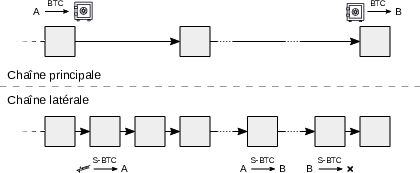
\includegraphics{chapters/img/sidechain-two-way-peg.png}

}

\caption{Sidechain: deposit, transfer, and withdrawal.}

\end{figure}%

The second aspect concerns transaction confirmation on the sidechain,
where options are more varied. The consensus can rely on merged mining,
in which case the main chain's work is used. It can be based on
proof-of-stake, involving the main chain's unit. Or it can use a
federation agreeing through a classical BFT algorithm, in which case
membership in this federation matters (proof-of-authority).

This vision materialized with the launch on BTC of two distinct
sidechains in 2018. The first was RSK (also called Rootstock), launched
by Sergio Lerner in January that year, focused on running a
Turing-complete virtual machine close to Ethereum's. The second was
Liquid, the implementation of the Elements model developed by
Blockstream, whose primary goal was to facilitate transactions between
various financial actors in the sector, including exchanges. In Liquid,
security relies on a federation of functionaries performing both roles:
they maintain the L-BTC peg as watchmen and participate in the chain's
consensus as block signers. RSK combines merged mining and a federation
of ``notaries'' to ensure both the anchoring of RBTC and transaction
processing.

However, the two sidechains have not managed to attract significant
activity over the years due to associated risks. Indeed, using these
chains still requires a form of trust that, although minimized, remains
present. An unfortunate example of a sidechain gone wrong is the
SmartBCH sidechain of Bitcoin Cash, where the company managing the
largest bridge between the two chains, CoinFLEX, went bankrupt and could
not reimburse users.

To address these drawbacks and reduce the involved trust, a more
advanced protocol was developed by researcher Paul Sztorc since November
2015: Drivechain\footnote{Paul Sztorc, \emph{Drivechain - The Simple Two
  Way Peg}, November~24, 2015:
  \url{https://www.truthcoin.info/blog/drivechain/}.}. As its name
suggests (drive chain meaning transmission chain), it is a true machine
for creating and managing sidechains.

Drivechain's main feature is that the two-way peg is entrusted to
miners, through hashrate escrow defined in BIP-300. During each
six-month period (26,300~blocks), miners vote for the sidechain
withdrawal transaction distributing funds to users who requested it. The
transparency and slowness of these transactions allow all main chain
merchants to audit them. Regular, faster transfers are made via atomic
swaps or centralized services.

Transaction validation on a sidechain using Drivechain can be ensured by
any consensus algorithm. But the most natural is to use merged mining.
That's why the Drivechain project also includes the proposal for
``blind'' merged mining (BIP-301), a technique allowing main chain
miners to automatically delegate sidechain validation to others in
exchange for remuneration. The validator earns the difference between
the sidechain's revenue and the purchase of the ``right to find a
block.'' This has the effect of not obliging miners to manage sidechains
while still receiving part of their revenue.

Drivechain is a clever concept that would fully realize Blockstream's
2014 vision. However, it has a major drawback: the security model of its
two-way peg. It relies on the potential recourse to a soft fork carried
out by merchants to correct a fraudulent withdrawal transaction, which
could, for example, be the doing of malicious miners seeking to steal
the escrowed funds. It thus depends on merchants' propensity to monitor
the sidechain's activity on one hand, and to proceed with a protocol
modification to freeze the incriminated transaction on the other. This
is why the proposal is, even today in 2023, hotly disputed.

\section*{The Lightning Network}\label{the-lightning-network}
\addcontentsline{toc}{section}{The Lightning Network}

\markright{The Lightning Network}

The Lightning Network is a concept of a network of bidirectional payment
channels. It was first presented on February~23, 2015, by Joseph Poon
and Thaddeus Dryja during a Bitcoin developers' seminar in San
Francisco\footnote{Taariq Lewis, \emph{SF Bitcoin Devs Seminar: Scaling
  Bitcoin to Billions of Transactions Per Day}, March~5, 2015:
  \url{https://www.youtube.com/watch?v=8zVzw912wPo}.}. At the time,
competing proposals based on similar ideas existed, such as Amiko Pay
(conceptualized by Corné Plooy), Impulse (developed by Jeff Garzik for
Bitpay), and Ström (imagined by the startup Strawpay), but Lightning
quickly became dominant. In 2023, it was the favored solution by BTC
users to perform more transfers, so much so that the acronym LNP/BP
emerged to designate all protocols involved in layering (akin to TCP/IP
for the Internet).

The Lightning Network infrastructure relies on payment channels opened
and closed between participants. A payment channel is, as described in
Chapter~\hyperref[ch:contrats]{13}, a set of smart contracts that allows
two people to make repeated payments safely and instantly from
previously locked liquidity. The use of a channel is therefore limited
by its capacity, that is, the sum of both actors' balances.

The principle of the Lightning Network is to route payments through
these channels via HTLCs, which are more complex commitment contracts
allowing the involved channels to be updated\footnote{In practice, these
  HTLCs are often also used to update the channels directly, to simplify
  implementation and improve privacy. --- See Andreas M. Antonopoulos,
  Olaoluwa Osuntokun, René Pickhardt, ``Routing on a Network of Payment
  Channels,'' in \emph{Mastering the Lightning Network: A Second Layer
  Blockchain Protocol for Instant Bitcoin Payments}, O'Reilly Media,
  2022, pp.~185--207.}. A payment transits over the network with minimal
fees that go to the nodes relaying it. The Lightning Network is thus
akin to an abacus, where the rods are channels and the beads are
satoshis moving from one side to the other of the channels, as shown in
Figure~\hyperref[fig:lightning-network-abacus]{14.2}.

\begin{figure}

{\centering 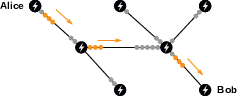
\includegraphics{chapters/img/lightning-network-abacus.png}

}

\caption{Payment of 3~mBTC on the Lightning Network.}

\end{figure}%

This functioning offers the possibility of making almost instantaneous
and cheap payments. It allows more bitcoin transfers without making more
transactions on-chain and without explicitly delegating fund management
to a third party. Moreover, the model retains all of Bitcoin's
programmability and opens up possibilities for monetary use on the
Internet.

However, Lightning's benefits should be tempered because it is not
without flaws. First, it inherits drawbacks related to the payment
channel model where, in the case of the Poon-Dryja protocol, an error
can lead to loss of funds. Then, constraints related to capacity and
routing necessarily create a tendency toward centralization, notably
through the emergence of so-called Lightning Service Providers, which
could lead to censorship. Furthermore, contrary to popular belief,
privacy on Lightning is weak, as payments are made between identified
public keys and transit through intermediaries. Finally, the network is
subject to the fee level on the main chain, necessary for contract
settlement, which limits the additional transaction capacity provided.

The Lightning Network is therefore suitable for handling everyday
payments and micropayments that do not necessarily require the
confidentiality and censorship resistance offered by the blockchain,
using well-funded channels that are regularly replenished. It was
implemented from January~2018, mainly as an overlay on BTC, and has
grown considerably since, both technically and economically. Three
software implementations were maintained by three different entities
(lnd by Lightning Labs, c-lightning by Blockstream, eclair by ACINQ),
and a system of technical standards (called Bases of Lightning
Technology or BOLT) eventually emerged. Economically, the network met
with some success by attracting capital, and in November~2023, a total
capacity of 5,400~BTC, equivalent to about 200 million dollars, was
reserved to provide liquidity for payments.

\section*{Fedimint Chaumian Banks}\label{fedimint-chaumian-banks}
\addcontentsline{toc}{section}{Fedimint Chaumian Banks}

\markright{Fedimint Chaumian Banks}

Another proposal is Fedimint\footnote{The functioning of Fedimint is
  described in the documentation on the website:
  \url{https://fedimint.org/docs/intro}.}, a protocol for custody and
confidential exchange of bitcoins in a community context. Technically,
it involves entrusting bitcoin custody to a federation and exchanging
Chaumian tokens (eCash) issued by that federation. This functioning
explains the protocol's name, which is an approximate abbreviation of
Federated Chaumian Mint.

Fedimint was envisioned by cypherpunk Eric Sirion during 2021 and
implemented in minimal form under the name MiniMint. Sirion was doubly
inspired by attempts to apply eCash as a Bitcoin overlay like SCRIT and
by community approaches such as Bitcoin Beach in El Salvador. The first
transaction of a Fedimint federation took place on September 28, 2022,
during the Hackers Congress at Paralelni Polis.

The first component of Fedimint is the Chaumian bank managed by the
federation. It uses David Chaum's blind signature process to issue
certificates backed by a certain amount of satoshis, which can be
redeemed at any time on-chain or on the Lightning Network. This
component provides partial financial privacy to participants: the bank
is unaware of exchanges made by clients, but its role in preventing
double-spending requires it to see merchants' revenues\footnote{The
  technical functioning of Chaumian systems was described in the section
  ``eCash: Chaumian Cash'' of Chapter~\hyperref[ch:cybermonnaie]{6}.}.

The idea of using eCash as a Bitcoin overlay is not new. It was proposed
and implemented for the first time on August~17, 2010, by an individual
operating under the pseudonym fellowtraveller on the Bitcoin forum in
the form of his project Open Transactions. The project never took hold,
as the need was not felt and the system was probably too complex.
However, the idea timidly resurfaced during the scalability debate with
the proposal of ``bearer blind certificates'' by Theymos (administrator
of the r/Bitcoin subreddit and the Bitcointalk forum) in December~2016.
It was also taken up in 2019 by Frank Braun and Jonathan Logan (co-hosts
of the Cypherpunk Bitstream podcast) through SCRIT, a federated Chaumian
system project whose name is the acronym for Secure, Confidential,
Reliable, Instant Transactions. The latest project to implement a
centralized Chaumian system is Cashu, a protocol developed in 2022 by
developer callebtc, allowing the creation and exchange of bitcoin
certificates on top of Lightning and new tokens.

Fedimint's interest, just like its predecessor SCRIT, is to decentralize
bitcoin custody. To do this, it combines the Chaumian system with a
so-called ``community'' approach, consisting of deploying a bank managed
by trusted members of a local community.

This approach was illustrated by the Bitcoin Beach experiment, a
sustainable economic development project around El Zonte beach in El
Salvador. A community bank emerged in 2020 and has since allowed locals
to exchange bitcoins safely and reliably, via the Bitcoin Beach Wallet
(now Blink) developed by Galoy. This experience inspired the adoption of
legal tender at the national level in September~2021.

The second component of Fedimint is therefore a federation, similar to
the federations of sidechains like Liquid or RSK, but composed of
trusted individuals with the technical capabilities necessary to operate
a node. These federation members, called guardians, are responsible for
setting up the infrastructure and are in charge of storing users' funds
and ensuring the proper functioning of the Chaumian bank. They
coordinate using a classical consensus algorithm (called HBBFT), which,
like all such algorithms, requires at least 66\% honest actors to
function.

Using this federation represents an obvious technical compromise between
full ownership of funds and their delegation to a single actor. This
compromise brings major advantages in terms of transaction processing
fees and ease of use but also entails significant risks. These are
custody risk (the federation can steal or lose funds), fraudulent
issuance risk (it can issue more certificates than it has bitcoins),
censorship risk (it can refuse to validate a transaction), and
regulatory risk (the federation can be seized and shut down by state
decision).

All this means that Fedimint cannot be conceived as a scalability
solution but as a proposal to replace custodial applications. Fedimint's
goal is to improve bitcoin custody by decentralizing it and increasing
the confidentiality of internal exchanges. Its local character should
allow it to escape financial regulations and thus avoid the fate
reserved for traditional banks.

\section*{Scaling Through
Substitution}\label{scaling-through-substitution}
\addcontentsline{toc}{section}{Scaling Through Substitution}

\markright{Scaling Through Substitution}

Layering is a correct way to increase the economic volume related to a
given chain without overly affecting its primary characteristics.
Nevertheless, this approach also has limits: not only do the various
overlays have their own flaws, but they ultimately rely on settlements
made on the blockchain, whose capacity is limited. Consequently, the
utility floor is not eliminated by layering, and thus it cannot be seen
as a miraculous way to handle an infinite number of transactions.

The range of values served by a given cryptomonetary system results in
demand for substitution systems better able to handle transfers outside
this range. A system with a high fee level leaves the way open for using
a less secure but cheaper system, allowing the processing of smaller
transactions. Conversely, a system with low security level favors the
emergence of a more expensive but also more secure system, enabling
larger transfers. Therefore, there is a certain complementarity between
the different implementations of Bitcoin that allow managing all
transaction activity emanating from users\footnote{Eric Voskuil,
  ``Substitution Principle,'' in \emph{Cryptoeconomics: Fundamental
  Principles of Bitcoin}, Amazon KDP, 2022, pp.~315--316.}.

Throughout history, such complementarity has manifested through the use
of several precious metals as monetary base. Gold could not cover all
value ranges: it was suitable for transferring large sums, for which it
was selected as the world's reserve currency, but not for exchanging
small change. To fulfill this latter complementary role, silver, and
other less precious metals like copper, were used. Silver, a word still
used today in French as a synonym for money, was the currency of
everyday life, while gold was mainly used for more expensive
settlements.

This bimetallic (or even trimetallic) aspect of money persisted for
centuries, from the High Antiquity to the 19th~century. It was
recognized by public authorities who defined their currency as a weight
in gold or silver, and minted gold and silver coins by decreeing an
exchange rate according to the gold-silver market ratio. Moreover, we
observe that this gold-silver ratio was relatively stable throughout
history, varying between 10 and 18, confirming silver's monetary role
alongside gold.

However, with the emergence of the gold standard and the disappearance
of bimetallism at the end of the 19th~century, silver gradually lost its
monetary role to be replaced by paper money, initially backed by gold,
much more convenient for exchanges. The ratio consequently increased
from 15.5 in 1870 to 80 today, corresponding to a loss of silver's value
of over 80\% relative to gold.

The analogy with precious metals is enlightening. Since the main version
of Bitcoin (BTC) is not suitable for processing smaller value transfers,
it follows that these potential transfers are carried out using a
substitute currency (cryptocurrency, fiat cash, credit moved by
permissive banking services, etc.) or are not processed at all.
Litecoin, whose main narrative is that it would be digital silver just
as Bitcoin is digital gold, perfectly meets this demand. It was thus
presented from its launch as a ``lighter version of Bitcoin'' aiming to
be ``to silver what Bitcoin is to gold\footnote{Charlie Lee, \emph{Re:
  {[}ANN{]} Litecoin - a lite version of Bitcoin. Be ready when it
  launches!}, October~9, 2011, 06:14:28 UTC:
  \url{https://bitcointalk.org/index.php?topic=47417.msg564414\#msg564414}.}.''
This designation stems not so much from the fact that there are four
times as many litecoins as bitcoins, which has no impact on the system,
but rather from the fact that LTC's maximum transaction capacity is four
times greater, which reduces the system's potential security. This
analysis also applies to Bitcoin Cash on an even larger scale.

In this view, alternative implementations of Bitcoin would serve to
process all transactions, at the price of necessary transfers between
chains. These would be ensured by centralized exchange services or by
atomic swap systems based on public order books. This solution, although
imperfect, would be entirely natural and is indeed already practiced
today.

Extensibility is also affected by this effect. The technical cost of
complex use of Bitcoin can be compensated by lower-quality substitution
systems. Low-cost confidentiality can be provided by Monero and
simplified programmability by Ethereum Classic, for example. As Satoshi
Nakamoto very aptly observed in December~2010 regarding the relevance of
BitDNS (the future Namecoin):

``Putting all proof-of-work quorum systems into one dataset doesn't
scale. Bitcoin and BitDNS can be used separately. {[}\ldots{]} The
networks need to be able to grow and die separately. Users of BitDNS
might be extremely liberal about adding features that bloat the chain,
since not many DNS root servers are needed, whereas Bitcoin users might
get increasingly conservative about keeping the blockchain small so that
it's easy for lots of users and small devices\footnote{Satoshi Nakamoto,
  \emph{Re: BitDNS and Generalizing Bitcoin}, December~10, 2010,
  17:29:28:
  \url{https://bitcointalk.org/index.php?topic=1790.msg28917\#msg28917}.}.''

\section*{Three Types of Compromises}\label{three-types-of-compromises}
\addcontentsline{toc}{section}{Three Types of Compromises}

\markright{Three Types of Compromises}

Bitcoin's scalability is a complex subject. Contrary to what is
sometimes claimed, a given system is hardly scalable. Its ability to
scale up can only be improved through software, hardware, or algorithmic
optimizations. Performance gains on the chain most often come at the
price of a direct compromise, with increasing the transaction capacity
limit, or an indirect one, with altering the security model.

This is the reason for the existence of layering, which involves
offloading part of the economic transfers to open and decentralized
protocols, partially preserving Bitcoin's properties and relying on
dispute settlement on the chain. In this approach, the security
compromise is partial and time-limited, unlike the transaction capacity
increase where it is total and persistent. Layering has developed on BTC
over time through sidechains, proposed in 2014 and implemented in 2018;
the Lightning Network, proposed in 2015 and deployed since 2018; and
Fedimint, proposed in 2021.

The other alternative is scaling through substitution, which essentially
involves moving less risky transactions to lower-quality substitutes,
that is, less secure implementations of the Bitcoin concept. This effect
truly manifested for the first time in 2017 with the initial congestion
on the BTC network and the rise in demand for static smart contracts
(Ethereum), which notably accompanied a decrease in the economic
dominance of Bitcoin's main version. Maximalists tend to claim that
layering allows handling all relevant uses of Bitcoin, but, until proven
otherwise, this is not the case.

\bookmarksetup{startatroot}

\chapter{The Future of Bitcoin}\label{ch:avenir}

\phantomsection\label{enotezch:15}{}

{S}\textsc{atoshi} Nakamoto's discovery of Bitcoin marks a profound
conceptual revolution in monetary systems. This explains why, since
2008, it has ignited intense passions among both its supporters and
critics. Some have seen it as the solution to all the world's
problems---a universal currency destined to replace gold and all fiat
money without opposition. Others have tried to depict it as a harmful,
polluting scheme of organized fraud, expressing an instinctive rejection
characteristic of the institutions they represented.

In this book, we have aimed to offer a balanced perspective by
thoroughly exploring where Bitcoin comes from, the challenges it faces,
and the principles that underpin it. Due to its design, Bitcoin stands
as a remarkably elegant tool whose mechanisms warrant detailed
examination---a task we have undertaken here. By way of conclusion,
let's recap what we have explored before turning our attention to
Bitcoin's future.

\section*{The Elegance of Bitcoin}\label{the-elegance-of-bitcoin}
\addcontentsline{toc}{section}{The Elegance of Bitcoin}

\markright{The Elegance of Bitcoin}

To begin with, it's important to remember that Bitcoin didn't appear out
of thin air. It's the product of technological advancements during the
latter half of the 20th century, heavily reliant on personal computers,
asymmetric cryptography, and the Internet. Ideologically, it draws from
diverse movements such as agorism, open-source advocacy, and
extropianism, all of which emphasized practical action over mere
theorizing. Specifically, it evolved from the cypherpunk movement,
which, starting in the early 1990s, endorsed the proactive use of
cryptography to safeguard privacy and individual rights in the emerging
cyberspace. Thus, the fundamental value underpinning Bitcoin is freedom.

Furthermore, Bitcoin is the culmination of an extensive pursuit of
digital currency, a quest notably championed by the cypherpunks. It owes
a debt to Chaum's eCash system, which enjoyed brief prominence in the
mid-1990s before disappearing. It also takes cues from private digital
currency endeavors such as Liberty Dollar, e-gold, and Liberty Reserve,
all of which were halted by governments in the early 21st century.
Bitcoin aligns with the lineage of decentralized currency concepts like
b-money, Bit Gold, RPOW, and, to some degree, Ripple.

Satoshi Nakamoto conceived Bitcoin in 2007, publishing its seminal white
paper on October 31, 2008, before finalizing the prototype and launching
the network in January 2009. Following a rocky beginning, the
cryptocurrency gradually emerged from obscurity, drawing in individuals
intrigued by its potential. These pioneers contributed to Bitcoin's
growth by engaging in software development, mining, and commerce. Once
the project was fully launched in 2010, Satoshi gradually vanished,
handing over control to his trusted collaborators. To this day, his
anonymity remains intact.

With the founder gone, the community had to self-organize. This era saw
the first conferences, initial debates about the protocol's future, and
the development of the earliest lightweight wallets. However, the
decentralization of Bitcoin's development eliminated any singular
dominant perspective, leading to numerous conflicts, beginning with the
P2SH controversy in 2011--2012. Four significant divides surfaced:
first, financialization---the partial reintroduction of trusted third
parties; second, scaling issues---deciding between increasing the
blockchain's transaction capacity or employing layer-two solutions;
third, the emergence of alternative cryptocurrencies, fiercely
criticized by some and welcomed by others; and fourth, institutional
integration---whether to cooperate with or oppose authority. These
conflicts have shaped Bitcoin into what it is today.

Bitcoin represents a new form of currency. It is a medium of exchange
with distributed management, meaning it doesn't depend on a central
authority. Although its resistance to change aligns it somewhat with
tangible goods, Bitcoin isn't a commodity currency since its attributes
don't derive from intrinsic physical properties. Even though it shares
the digital nature of the banking system, it's not a ledger-based
currency, as its ledger entries don't represent claims. While it lacks
significant non-monetary uses, it's not centralized fiat money because
it doesn't depend on trust in a single actor. Ultimately, Bitcoin falls
into a new category and can be described as a network currency or
distributed fiat currency, meaning it disperses trust across a network
of nodes operated by merchants rather than concentrating it with a
single entity.

Bitcoin is a ``peer-to-peer electronic cash system'' enabling ``online
payments to be sent directly from one party to another without the need
for a financial institution.'' It represents a digital currency concept
resistant to censorship and inflation, making it challenging to obstruct
transactions or create additional units. Bitcoin is a tool naturally
suited to the margins, operating at the boundary of legality, and
sometimes beyond. It's a currency of dissent, employed by political
activists, whistleblowers, and organizations that challenge authority.
It's a currency of freedom for censored individuals---those whose
professions are considered deviant, who dare to voice dissenting
opinions, or who were unfortunate enough to be born in the wrong
country. It's a black-market currency utilized by the underground
economy, particularly in acts of tax resistance.

This role as a currency of freedom puts it at odds with the state, which
inherently seeks continual expansion, particularly by tightening its
grip on money. By supervising banking, the state has altered the
foundation of money, shifting it from precious metals to fiat coins and
bills. It could repeat this by converting physical currency into a
central bank digital currency accessible to all, subject to pervasive
surveillance and censorship. This predatory stance of the state
underpins Bitcoin's distributed architecture, which disperses risks
among system participants, endowing it with unprecedented robustness.

Bitcoin relies on several technical components to operate effectively.
The foremost is digital signatures, which secure ownership within the
system. Users truly own their bitcoins by exercising exclusive control
over their private keys. This mechanism grants the unique freedom of
sovereignly managing digital funds but also demands responsibility
concerning loss and theft---risks absent when dealing with a trusted
third party.

To prevent double-spending, Bitcoin employs an innovative consensus
algorithm that updates a chain of time-stamped transaction blocks
through a proof-of-work process. Its open and robust operation sets it
apart from traditional consensus algorithms previously used in
distributed systems. Nakamoto's brilliance lay in sacrificing some
security (rendering it probabilistic rather than absolute) to achieve
Byzantine fault tolerance. This model hinges on miners' economic
incentives---they find it more profitable to mine the chain legitimately
than to attack it.

However, the genius of Bitcoin's design doesn't stop there. It not only
discourages double-spending but also combats financial censorship---a
significant issue in today's digital transactions. Censorship in Bitcoin
involves mining a longer chain that omits undesirable transactions.
Thanks to integrated transaction fees and the external nature of
proof-of-work, such suppression can be effectively contested, aligning
with the model's resistance to censorship.

Bitcoin is an open and free concept of currency, inherently dynamic and
multifaceted. Consequently, a variety of Bitcoin implementations exist,
influenced by two opposing effects: network effect and substitution
effect. The monetary nature of Bitcoin suggests that only a few
implementations can survive, while its lack of scalability implies that
multiple versions may persist.

Determining the protocol---or protocols---is an economic process driven
by merchants' acceptance of the currency. Merchants play the most
crucial role by having the final say on consensus rules through their
economic activity verified by their nodes. More broadly, the governance
model is sociologically complex; merchants are influenced by other
system participants like customers, holders, developers, and miners, as
well as external actors such as opinion leaders, financial powers, and
the state.

Resistance to inflation---or the difficulty in creating more
bitcoins---emerges from the economic dynamics opposing changes to
monetary policy. It doesn't stem from a lack of community unanimity or
Satoshi Nakamoto's original establishment of the monetary policy. The
emblematic 21 million limit isn't absolute; it depends at every moment
on merchants' decisions.

Technically, Bitcoin is optimized for currency use, as evidenced by its
unit representation model based on coins rather than accounts like
Ethereum. While no advanced techniques were integrated into the
prototype, Bitcoin is also designed for privacy, as preserving privacy
is essential for currency fungibility and resistance to censorship.

Moreover, Bitcoin is programmable, allowing spending conditions to be
imposed on different coins. This modular aspect of transactions enables
strangers to exchange value as confidentially and securely as possible.
It's also the foundation for layer-two protocols like the Lightning
Network, which increase exchange capacity without compromising the base
system's security.

All these properties make Bitcoin a cohesive whole of rare elegance.
Bitcoin is the missing piece of the puzzle for freedom on the Internet.
Bitcoin represents the hope of a generation facing ever-growing state
authority. Bitcoin embodies the project of a robust and sustainable
alternative monetary system, explaining the tremendous momentum it
enjoyed in its early years.

\section*{The Four Threats Facing
Bitcoin}\label{the-four-threats-facing-bitcoin}
\addcontentsline{toc}{section}{The Four Threats Facing Bitcoin}

\markright{The Four Threats Facing Bitcoin}

As we've discussed throughout this book, Bitcoin isn't entirely shielded
from adversarial attacks. In this section, we'll outline the main
threats looming over Bitcoin today. We'll avoid technical risks, which
have been addressed by more knowledgeable individuals, and focus solely
on dangers arising from human behavior---specifically actions by
economic actors within the system. In our view, these pose far greater
concern.

Human threats are subtle because the attacks they enable often occur
suddenly. The increase of these threats resembles a game of musical
chairs, where participants naively circle chairs without monitoring
them. As long as the music plays, all seems well---the adversary calmly
removes chairs one by one, and the circle continues. It's only when the
music stops that problems become apparent.

We identify four such threats that could harm Bitcoin: centralization of
economic activity, centralization of mining activity, widespread
custodial holdings, and erosion of privacy. These threats aren't
entirely independent but correspond to different behaviors among actors.

The first threat is the centralization of economic activity, emerging
through significant commerce conducted via regulated exchanges and the
near-universal use of external payment processors and third-party wallet
providers. This could lead, as described in
Chapter~\hyperref[ch:determination]{11}, to protocol alteration attacks
in the form of an inflationary hard fork, a tax-based soft fork, or a
censorship soft fork. Such attacks might cause a chain split in one way
or another and are especially damaging if the altered chain becomes
dominant due to network effects. However, the attack isn't fatal to the
system since the economy can gradually rebuild on the free chain.

The second threat is the centralization of mining activity, evident in
the geographical clustering of mining equipment, the grouping of hashers
into cooperatives, and miners' collective use of centralized relay
networks. This risk could lead, as seen in
Chapter~\hyperref[ch:censure]{9}, to transaction censorship attacks by a
majority of the network's computing power. Such an attack is likely to
occur after an attempted protocol alteration on the free chain that
refused the changes. It effectively paralyzes part of the activity by
preventing its confirmation on the chain. The attack benefits from chain
analysis to isolate problematic transactions rather than suppress all
activity. However, it's not fatal to the system, as additional mining
equipment can be deployed---spurred by increased fees from censored
transactions---to restore the initial situation.

The third threat, related to the centralization of economic activity, is
the widespread custodial holding of funds by entities adhering to legal
regulations. Not only is this practice individually questionable (a
custodian can censor transactions, seize funds, and inflate the number
of paper bitcoins they distribute), but its proliferation creates
systemic risk. This threat manifests today through the growth of
institutional custodians like Coinbase Custody holding a significant
percentage of circulating bitcoins and the expansion of services
targeting small investors. It's more dangerous than economic
centralization because a ``hosted'' economy cannot reform if there's a
protocol attack---the regulated custodians are the actual bitcoin
owners, not their clients. This represents a persistent degradation of
the system, harder to rectify than mere mining or commercial
centralization.

The fourth, more insidious threat is the erosion of privacy,
materializing through widespread surveillance (know-your-customer
protocols, proof of address ownership) and, incidentally, accompanying
chain analysis. Similar to custodial holding by regulated entities,
complete transparency to the state is not only an individual misstep
(leaving one unprotected from censorship and seizure) but also a
systemic risk if it becomes widespread. Greater surveillance creates a
more controllable economy, making the protocol more vulnerable.
Additionally, identifying actors reduces the anonymity set benefitting
everyone and diminishes the possibility of conducting secret activities.
The erosion of privacy thus becomes a subtle system degradation that can
only be remedied by combating identification links through good
practices like coin mixing.

These threats depend on the actions of Bitcoin's economic actors,
especially its users. To combat them, users should be encouraged to
withdraw their bitcoins to personal wallets, avoid compliance with
know-your-customer protocols, make their bitcoins untraceable, and use
their own nodes---individually or within communities. This is
particularly relevant for new users, leading us to the topic of
adoption.

\section*{The Two Paths of Cryptocurrency
Adoption}\label{the-two-paths-of-cryptocurrency-adoption}
\addcontentsline{toc}{section}{The Two Paths of Cryptocurrency Adoption}

\markright{The Two Paths of Cryptocurrency Adoption}

Bitcoin is a system based on economic incentives where those who sustain
it are rewarded. Miners are incentivized to confirm transactions to earn
fees. Merchants are incentivized to verify consensus rules to fully
benefit from Bitcoin's value proposition. Holders are incentivized to
promote Bitcoin to expand the economy and enjoy the resulting increase
in purchasing power (or dollar price) of the unit of account. This
economic expansion, or adoption, is thus a natural goal for those who
own bitcoin.

There are numerous ways Bitcoin can be adopted, but two primary models
stand out. The first is adoption by individuals and small businesses,
representing a modest financial contribution to bitcoin's aggregate
value. The second is adoption by large corporations, brokerage firms,
and financial institutions, offering a more significant gain for
holders. In the early days, convincing the latter group of bitcoin's
merits was impossible, but with economic development and tailored
communication, persuading them to participate has become much easier.
Since this adoption was more profitable for holders, many chose the path
of least resistance, filling their discourse with language aimed at
regulated actors.

However, this second wave of bitcoin adoption, while profitable in the
short term and possessing its own merits, tends to become sterile in the
long run. It creates a centralized, monitored, and even entirely
custodial economy---an economy fragile and at the mercy of governmental
decisions. Therefore, we can term it ``bad adoption.''

The only adoption worth pursuing is that of a free and independent
economy for which Bitcoin is inherently suited. This economy possesses
characteristics that allow Bitcoin to endure. It is decentralized,
distributing risks among all its members to maximize Bitcoin's value
proposition. It is disobedient, refusing any protocol modifications that
would alter Bitcoin's fundamental properties. It safeguards its privacy,
aware that surveillance poses a threat even when no immediate illegal
activity is involved. It is circular, minimizing reliance on
state-issued money, especially in digital form, sensing that such
currency is increasingly controlled. Finally, it is demanding, requiring
discernment and responsibility from individuals---qualities often
overlooked in our modern era.

However, the constraints of this ``good adoption'' make it inaccessible
to everyone. Not only does sovereign Bitcoin use demand a degree of
responsibility, but it also presents significant drawbacks, currently
including purchasing power volatility, transaction costs, lack of
scalability, and discouraging regulations. Therefore, expecting everyone
to adopt bitcoin as their preferred currency in the short or medium term
is unrealistic. In other words, mass adoption won't happen anytime soon,
and Bitcoin use will initially remain confined to those seeking to
escape the state-banking system and resist the powers that be.

It's thus illusory to anticipate ``hyperbitcoinization,'' a rapid
replacement of fiat currencies by bitcoin. As long as there exists a
mass of people who blindly obey authority, state-issued money will
persist. Only necessity might drive this mass to make opportunistic and
temporary use of Bitcoin.

\section*{A Culture in the Making}\label{a-culture-in-the-making}
\addcontentsline{toc}{section}{A Culture in the Making}

\markright{A Culture in the Making}

Culture encompasses the material, intellectual, emotional, and spiritual
aspects that characterize societies or social groups. Every enduring
human association tends to develop its own culture. The Bitcoin
community, though vaguely defined, is no exception. Cultural elements
emerged in Bitcoin from its inception and multiplied as the network
grew, eventually giving rise to a genuine subculture.

This culture is inherently political, marked by animosity toward
authority figures and numerous references to cypherpunks and Austrian
economists. It also comprises ritualized monetary practices, hygiene
recommendations (notably against dubious crypto-assets), futuristic
artworks, books, and various podcasts, gatherings (monthly meetups,
conferences), and regular commemorations of events that have shaped
cryptocurrency history. The culture of Bitcoin---the Internet's
currency---also heavily relies on concise slogans and humorous memes,
particularly suited for propagation on social media.

Culture, especially the religious facet, influences individual actions.
Since Bitcoin is a tool whose security depends on how it's used, this
cultural aspect is fundamental. For example, the phrase ``not your keys,
not your bitcoins,'' coined by Andreas Antonopoulos, is far more
convincing in encouraging people to store funds in personal wallets than
any historical account of platform failures and account freezes.
However, culture can also misguide behavior, ultimately harming the
system.

As a speculative asset whose price has multiplied 30 million times over
14 years, bitcoin has attracted those eager for financial gain. It
boasted absolute scarcity by design---a novelty in history---and it's
natural that this drew attention. This was one of Satoshi Nakamoto's
essential choices, as this speculative appeal partly facilitated the
monetization process and introduced Bitcoin to individuals who might
have otherwise ignored it.

However, Bitcoin's culture was profoundly influenced in the process. A
genuine trend toward greed emerged within the community, reflected in
memes and various slogans. Notably, there's an underlying assumption
that ``the number must go up,'' propelling the price ``to the moon,''
based on the notion that the world's wealth is infinite and there are
only 21 million bitcoins (\(\infty / 21\mathrm{M}\)). Consequently,
individuals should ``stack sats'' (accumulate satoshis) and ``HODL''
(hold on for dear life) to benefit from a better future. This mindset is
evident in representations of Bitcoin and bitcoiners, such as the bull
of the bullish market or laser eyes (\#LaserRayUntil100K).

This desire for an ever-higher price relies on the delusion of mass
adoption we've discussed earlier. For the price to reach lofty heights,
everyone must eventually possess bitcoin in some form. Since most people
aren't ready to use Bitcoin sovereignly, this adoption has been
facilitated through custodians. Thus, a culture centered on financial
gain led to the subtle weakening of Bitcoin by broadly accepting
financial intermediaries, consenting to mass identification, and
promoting Bitcoin to institutions and states.

Mass adoption isn't a realistic goal in the short or medium term. When
we extol Bitcoin's virtues, we're not addressing the masses per se;
we're reaching out to those who understand the issues it solves and
might be interested. Therefore, it's essential not to sanitize the
message---to not lose these individuals, we must tell the truth; and
while this truth can be veiled, it should never be distorted.

Bitcoin thrives on the tension between the official economy, which
approves monetary control, and the counter-economy, which opposes it.
Due to this tension, the cryptocurrency culture is constantly under
attack, notably by mass media, central bankers, and state
representatives. A staggering number of detractors, working for the
adversary, tirelessly repeat their disingenuous arguments. While it's
useful to confront them to set the record straight for a doubtful
audience, it's futile to believe they'll disappear or lose visibility.
Therefore, Bitcoin needs a tradition---a cultural transmission from
individual to individual---that can organically and healthily explain
its principles to newcomers.

Specifically, Bitcoin's message should always be a call to action, in
line with preceding ideological movements like the cypherpunks. Everyone
should feel encouraged to write (and read) code, deploy mining farms
when possible, participate in the circular economy, hold bitcoin, and
educate others on the subject, even if it doesn't bring direct financial
gain. This is also how Bitcoin prospers.

In any case, Bitcoin cannot be forgotten. Satoshi Nakamoto's discovery
is here to stay. It has already played a role in the fight for human
freedom and will likely play an even greater role in the future. Its
success will depend on the actions of those who support it. The
revolution will not be centralized.


\backmatter


\end{document}
